\documentclass[twoside]{book}

% Packages required by doxygen
\usepackage{calc}
\usepackage{doxygen}
\usepackage{graphicx}
\usepackage[utf8]{inputenc}
\usepackage{makeidx}
\usepackage{multicol}
\usepackage{multirow}
\usepackage{textcomp}
\usepackage[table]{xcolor}

% Font selection
\usepackage[T1]{fontenc}
\usepackage{mathptmx}
\usepackage[scaled=.90]{helvet}
\usepackage{courier}
\usepackage{amssymb}
\usepackage{sectsty}
\renewcommand{\familydefault}{\sfdefault}
\allsectionsfont{%
  \fontseries{bc}\selectfont%
  \color{darkgray}%
}
\renewcommand{\DoxyLabelFont}{%
  \fontseries{bc}\selectfont%
  \color{darkgray}%
}

% Page & text layout
\usepackage{geometry}
\geometry{%
  a4paper,%
  top=2.5cm,%
  bottom=2.5cm,%
  left=2.5cm,%
  right=2.5cm%
}
\tolerance=750
\hfuzz=15pt
\hbadness=750
\setlength{\emergencystretch}{15pt}
\setlength{\parindent}{0cm}
\setlength{\parskip}{0.2cm}
\makeatletter
\renewcommand{\paragraph}{%
  \@startsection{paragraph}{4}{0ex}{-1.0ex}{1.0ex}{%
    \normalfont\normalsize\bfseries\SS@parafont%
  }%
}
\renewcommand{\subparagraph}{%
  \@startsection{subparagraph}{5}{0ex}{-1.0ex}{1.0ex}{%
    \normalfont\normalsize\bfseries\SS@subparafont%
  }%
}
\makeatother

% Headers & footers
\usepackage{fancyhdr}
\pagestyle{fancyplain}
\fancyhead[LE]{\fancyplain{}{\bfseries\thepage}}
\fancyhead[CE]{\fancyplain{}{}}
\fancyhead[RE]{\fancyplain{}{\bfseries\leftmark}}
\fancyhead[LO]{\fancyplain{}{\bfseries\rightmark}}
\fancyhead[CO]{\fancyplain{}{}}
\fancyhead[RO]{\fancyplain{}{\bfseries\thepage}}
\fancyfoot[LE]{\fancyplain{}{}}
\fancyfoot[CE]{\fancyplain{}{}}
\fancyfoot[RE]{\fancyplain{}{\bfseries\scriptsize Generated on Wed Oct 29 2014 18\-:06\-:28 for libmae by Doxygen }}
\fancyfoot[LO]{\fancyplain{}{\bfseries\scriptsize Generated on Wed Oct 29 2014 18\-:06\-:28 for libmae by Doxygen }}
\fancyfoot[CO]{\fancyplain{}{}}
\fancyfoot[RO]{\fancyplain{}{}}
\renewcommand{\footrulewidth}{0.4pt}
\renewcommand{\chaptermark}[1]{%
  \markboth{#1}{}%
}
\renewcommand{\sectionmark}[1]{%
  \markright{\thesection\ #1}%
}

% Indices & bibliography
\usepackage{natbib}
\usepackage[titles]{tocloft}
\setcounter{tocdepth}{3}
\setcounter{secnumdepth}{5}
\makeindex

% Hyperlinks (required, but should be loaded last)
\usepackage{ifpdf}
\ifpdf
  \usepackage[pdftex,pagebackref=true]{hyperref}
\else
  \usepackage[ps2pdf,pagebackref=true]{hyperref}
\fi
\hypersetup{%
  colorlinks=true,%
  linkcolor=blue,%
  citecolor=blue,%
  unicode%
}

% Custom commands
\newcommand{\clearemptydoublepage}{%
  \newpage{\pagestyle{empty}\cleardoublepage}%
}


%===== C O N T E N T S =====

\begin{document}

% Titlepage & ToC
\hypersetup{pageanchor=false}
\pagenumbering{roman}
\begin{titlepage}
\vspace*{7cm}
\begin{center}%
{\Large libmae }\\
\vspace*{1cm}
{\large Generated by Doxygen 1.8.6}\\
\vspace*{0.5cm}
{\small Wed Oct 29 2014 18:06:28}\\
\end{center}
\end{titlepage}
\clearemptydoublepage
\tableofcontents
\clearemptydoublepage
\pagenumbering{arabic}
\hypersetup{pageanchor=true}

%--- Begin generated contents ---
\chapter{Hierarchical Index}
\section{Class Hierarchy}
This inheritance list is sorted roughly, but not completely, alphabetically\-:\begin{DoxyCompactList}
\item \contentsline{section}{mae\-:\-:fl\-:\-:angular\-\_\-joint}{\pageref{classmae_1_1fl_1_1angular__joint}}{}
\item \contentsline{section}{mae\-:\-:fl\-:\-:angular\-\_\-skeleton}{\pageref{classmae_1_1fl_1_1angular__skeleton}}{}
\item \contentsline{section}{mae\-:\-:math\-:\-:basis}{\pageref{classmae_1_1math_1_1basis}}{}
\item \contentsline{section}{mae\-:\-:bone}{\pageref{classmae_1_1bone}}{}
\item \contentsline{section}{mae\-:\-:fl\-:\-:bvh\-\_\-controller}{\pageref{classmae_1_1fl_1_1bvh__controller}}{}
\item \contentsline{section}{mae\-:\-:fl\-:\-:bvh\-\_\-data}{\pageref{classmae_1_1fl_1_1bvh__data}}{}
\item \contentsline{section}{mae\-:\-:fl\-:\-:bvh\-\_\-spec}{\pageref{classmae_1_1fl_1_1bvh__spec}}{}
\item \contentsline{section}{mae\-:\-:fl\-:\-:laban\-:\-:column\-\_\-definition}{\pageref{classmae_1_1fl_1_1laban_1_1column__definition}}{}
\item \contentsline{section}{mae\-:\-:fl\-:\-:laban\-:\-:decision\-\_\-forest}{\pageref{classmae_1_1fl_1_1laban_1_1decision__forest}}{}
\item \contentsline{section}{mae\-:\-:fl\-:\-:laban\-:\-:decision\-\_\-node$<$ T, U $>$}{\pageref{classmae_1_1fl_1_1laban_1_1decision__node}}{}
\item \contentsline{section}{mae\-:\-:fl\-:\-:laban\-:\-:decision\-\_\-tree$<$ T, U $>$}{\pageref{classmae_1_1fl_1_1laban_1_1decision__tree}}{}
\item \contentsline{section}{mae\-:\-:fl\-:\-:laban\-:\-:decision\-\_\-value$<$ T, U $>$}{\pageref{classmae_1_1fl_1_1laban_1_1decision__value}}{}
\item \contentsline{section}{mae\-:\-:fl\-:\-:laban\-:\-:ps\-:\-:e\-\_\-area\-\_\-c}{\pageref{classmae_1_1fl_1_1laban_1_1ps_1_1e__area__c}}{}
\item \contentsline{section}{mae\-:\-:e\-\_\-bone\-\_\-c}{\pageref{classmae_1_1e__bone__c}}{}
\item \contentsline{section}{mae\-:\-:fl\-:\-:laban\-:\-:mv\-:\-:e\-\_\-cancel\-\_\-c}{\pageref{classmae_1_1fl_1_1laban_1_1mv_1_1e__cancel__c}}{}
\item \contentsline{section}{mae\-:\-:fl\-:\-:laban\-:\-:mv\-:\-:e\-\_\-contact\-\_\-hook\-\_\-c}{\pageref{classmae_1_1fl_1_1laban_1_1mv_1_1e__contact__hook__c}}{}
\item \contentsline{section}{mae\-:\-:fl\-:\-:laban\-:\-:ps\-:\-:e\-\_\-digit\-\_\-c}{\pageref{classmae_1_1fl_1_1laban_1_1ps_1_1e__digit__c}}{}
\item \contentsline{section}{mae\-:\-:fl\-:\-:laban\-:\-:mv\-:\-:e\-\_\-direction\-\_\-c}{\pageref{classmae_1_1fl_1_1laban_1_1mv_1_1e__direction__c}}{}
\item \contentsline{section}{mae\-:\-:fl\-:\-:laban\-:\-:mv\-:\-:e\-\_\-dynamic\-\_\-c}{\pageref{classmae_1_1fl_1_1laban_1_1mv_1_1e__dynamic__c}}{}
\item \contentsline{section}{mae\-:\-:fl\-:\-:e\-\_\-fl\-\_\-direction\-\_\-c}{\pageref{classmae_1_1fl_1_1e__fl__direction__c}}{}
\item \contentsline{section}{mae\-:\-:fl\-:\-:e\-\_\-fl\-\_\-joint\-\_\-c}{\pageref{classmae_1_1fl_1_1e__fl__joint__c}}{}
\item \contentsline{section}{mae\-:\-:e\-\_\-joint\-\_\-c}{\pageref{classmae_1_1e__joint__c}}{}
\item \contentsline{section}{mae\-:\-:fl\-:\-:laban\-:\-:ps\-:\-:e\-\_\-joint\-\_\-c}{\pageref{classmae_1_1fl_1_1laban_1_1ps_1_1e__joint__c}}{}
\item \contentsline{section}{mae\-:\-:e\-\_\-kinect\-\_\-joint\-\_\-c}{\pageref{classmae_1_1e__kinect__joint__c}}{}
\item \contentsline{section}{mae\-:\-:fl\-:\-:laban\-:\-:mv\-:\-:e\-\_\-level\-\_\-c}{\pageref{classmae_1_1fl_1_1laban_1_1mv_1_1e__level__c}}{}
\item \contentsline{section}{mae\-:\-:fl\-:\-:laban\-:\-:ps\-:\-:e\-\_\-limb\-\_\-c}{\pageref{classmae_1_1fl_1_1laban_1_1ps_1_1e__limb__c}}{}
\item \contentsline{section}{mae\-:\-:fl\-:\-:laban\-:\-:ps\-:\-:e\-\_\-limb\-\_\-side\-\_\-c}{\pageref{classmae_1_1fl_1_1laban_1_1ps_1_1e__limb__side__c}}{}
\item \contentsline{section}{mae\-:\-:fl\-:\-:laban\-:\-:e\-\_\-path\-\_\-type\-\_\-c}{\pageref{classmae_1_1fl_1_1laban_1_1e__path__type__c}}{}
\item \contentsline{section}{mae\-:\-:fl\-:\-:laban\-:\-:e\-\_\-relationship\-\_\-type\-\_\-c}{\pageref{classmae_1_1fl_1_1laban_1_1e__relationship__type__c}}{}
\item \contentsline{section}{mae\-:\-:fl\-:\-:laban\-:\-:ps\-:\-:e\-\_\-side\-\_\-c}{\pageref{classmae_1_1fl_1_1laban_1_1ps_1_1e__side__c}}{}
\item \contentsline{section}{mae\-:\-:fl\-:\-:laban\-:\-:mv\-:\-:e\-\_\-space\-\_\-c}{\pageref{classmae_1_1fl_1_1laban_1_1mv_1_1e__space__c}}{}
\item \contentsline{section}{mae\-:\-:fl\-:\-:laban\-:\-:mv\-:\-:e\-\_\-space\-\_\-direction\-\_\-c}{\pageref{classmae_1_1fl_1_1laban_1_1mv_1_1e__space__direction__c}}{}
\item \contentsline{section}{mae\-:\-:fl\-:\-:laban\-:\-:e\-\_\-time\-\_\-unit\-\_\-c}{\pageref{classmae_1_1fl_1_1laban_1_1e__time__unit__c}}{}
\item \contentsline{section}{mae\-:\-:fl\-:\-:laban\-:\-:mv\-:\-:e\-\_\-turn\-\_\-direction\-\_\-c}{\pageref{classmae_1_1fl_1_1laban_1_1mv_1_1e__turn__direction__c}}{}
\item \contentsline{section}{mae\-:\-:general\-\_\-joint}{\pageref{classmae_1_1general__joint}}{}
\item \contentsline{section}{mae\-:\-:general\-\_\-pose}{\pageref{classmae_1_1general__pose}}{}
\begin{DoxyCompactList}
\item \contentsline{section}{mae\-:\-:general\-\_\-enriched\-\_\-pose}{\pageref{classmae_1_1general__enriched__pose}}{}
\end{DoxyCompactList}
\item \contentsline{section}{mae\-:\-:general\-\_\-skeleton}{\pageref{classmae_1_1general__skeleton}}{}
\begin{DoxyCompactList}
\item \contentsline{section}{mae\-:\-:fl\-:\-:fl\-\_\-skeleton}{\pageref{classmae_1_1fl_1_1fl__skeleton}}{}
\end{DoxyCompactList}
\item \contentsline{section}{mae\-:\-:hierarchy}{\pageref{classmae_1_1hierarchy}}{}
\item \contentsline{section}{mae\-:\-:hierarchy\-\_\-element}{\pageref{classmae_1_1hierarchy__element}}{}
\item \contentsline{section}{mae\-:\-:fl\-:\-:laban\-:\-:i\-\_\-decision\-\_\-maker$<$ T $>$}{\pageref{classmae_1_1fl_1_1laban_1_1i__decision__maker}}{}
\item \contentsline{section}{mae\-:\-:fl\-:\-:laban\-:\-:i\-\_\-decision\-\_\-maker$<$ i\-\_\-movement $>$}{\pageref{classmae_1_1fl_1_1laban_1_1i__decision__maker}}{}
\begin{DoxyCompactList}
\item \contentsline{section}{mae\-:\-:fl\-:\-:laban\-:\-:decision\-\_\-maker}{\pageref{classmae_1_1fl_1_1laban_1_1decision__maker}}{}
\item \contentsline{section}{mae\-:\-:fl\-:\-:laban\-:\-:rewriting\-\_\-decision\-\_\-maker}{\pageref{classmae_1_1fl_1_1laban_1_1rewriting__decision__maker}}{}
\end{DoxyCompactList}
\item \contentsline{section}{mae\-:\-:fl\-:\-:laban\-:\-:mv\-:\-:i\-\_\-degree\-\_\-sign}{\pageref{classmae_1_1fl_1_1laban_1_1mv_1_1i__degree__sign}}{}
\begin{DoxyCompactList}
\item \contentsline{section}{mae\-:\-:fl\-:\-:laban\-:\-:mv\-:\-:pin}{\pageref{classmae_1_1fl_1_1laban_1_1mv_1_1pin}}{}
\item \contentsline{section}{mae\-:\-:fl\-:\-:laban\-:\-:mv\-:\-:space\-\_\-measurement}{\pageref{classmae_1_1fl_1_1laban_1_1mv_1_1space__measurement}}{}
\end{DoxyCompactList}
\item \contentsline{section}{mae\-:\-:fl\-:\-:laban\-:\-:mv\-:\-:i\-\_\-dynamics\-\_\-sign}{\pageref{classmae_1_1fl_1_1laban_1_1mv_1_1i__dynamics__sign}}{}
\begin{DoxyCompactList}
\item \contentsline{section}{mae\-:\-:fl\-:\-:laban\-:\-:mv\-:\-:accent\-\_\-sign}{\pageref{classmae_1_1fl_1_1laban_1_1mv_1_1accent__sign}}{}
\item \contentsline{section}{mae\-:\-:fl\-:\-:laban\-:\-:mv\-:\-:dynamic\-\_\-sign}{\pageref{classmae_1_1fl_1_1laban_1_1mv_1_1dynamic__sign}}{}
\end{DoxyCompactList}
\item \contentsline{section}{mae\-:\-:i\-\_\-kp\-\_\-detector}{\pageref{classmae_1_1i__kp__detector}}{}
\begin{DoxyCompactList}
\item \contentsline{section}{mae\-:\-:kp\-\_\-detector}{\pageref{classmae_1_1kp__detector}}{}
\end{DoxyCompactList}
\item \contentsline{section}{mae\-:\-:fl\-:\-:laban\-:\-:i\-\_\-movement}{\pageref{classmae_1_1fl_1_1laban_1_1i__movement}}{}
\begin{DoxyCompactList}
\item \contentsline{section}{mae\-:\-:fl\-:\-:laban\-:\-:movement}{\pageref{classmae_1_1fl_1_1laban_1_1movement}}{}
\item \contentsline{section}{mae\-:\-:fl\-:\-:laban\-:\-:path}{\pageref{classmae_1_1fl_1_1laban_1_1path}}{}
\item \contentsline{section}{mae\-:\-:fl\-:\-:laban\-:\-:relationship\-\_\-bow}{\pageref{classmae_1_1fl_1_1laban_1_1relationship__bow}}{}
\item \contentsline{section}{mae\-:\-:fl\-:\-:laban\-:\-:room\-\_\-direction}{\pageref{classmae_1_1fl_1_1laban_1_1room__direction}}{}
\end{DoxyCompactList}
\item \contentsline{section}{mae\-:\-:i\-\_\-movement\-\_\-detector$<$ T, U $>$}{\pageref{classmae_1_1i__movement__detector}}{}
\begin{DoxyCompactList}
\item \contentsline{section}{mae\-:\-:kp\-\_\-movement\-\_\-detector$<$ T, U $>$}{\pageref{classmae_1_1kp__movement__detector}}{}
\end{DoxyCompactList}
\item \contentsline{section}{mae\-:\-:fl\-:\-:laban\-:\-:ps\-:\-:i\-\_\-part}{\pageref{classmae_1_1fl_1_1laban_1_1ps_1_1i__part}}{}
\begin{DoxyCompactList}
\item \contentsline{section}{mae\-:\-:fl\-:\-:laban\-:\-:ps\-:\-:i\-\_\-endpoint}{\pageref{classmae_1_1fl_1_1laban_1_1ps_1_1i__endpoint}}{}
\begin{DoxyCompactList}
\item \contentsline{section}{mae\-:\-:fl\-:\-:laban\-:\-:ps\-:\-:area\-\_\-part}{\pageref{classmae_1_1fl_1_1laban_1_1ps_1_1area__part}}{}
\item \contentsline{section}{mae\-:\-:fl\-:\-:laban\-:\-:ps\-:\-:digit\-\_\-part}{\pageref{classmae_1_1fl_1_1laban_1_1ps_1_1digit__part}}{}
\item \contentsline{section}{mae\-:\-:fl\-:\-:laban\-:\-:ps\-:\-:joint\-\_\-part}{\pageref{classmae_1_1fl_1_1laban_1_1ps_1_1joint__part}}{}
\end{DoxyCompactList}
\item \contentsline{section}{mae\-:\-:fl\-:\-:laban\-:\-:ps\-:\-:i\-\_\-limb}{\pageref{classmae_1_1fl_1_1laban_1_1ps_1_1i__limb}}{}
\begin{DoxyCompactList}
\item \contentsline{section}{mae\-:\-:fl\-:\-:laban\-:\-:ps\-:\-:custom\-\_\-limb}{\pageref{classmae_1_1fl_1_1laban_1_1ps_1_1custom__limb}}{}
\item \contentsline{section}{mae\-:\-:fl\-:\-:laban\-:\-:ps\-:\-:default\-\_\-limb}{\pageref{classmae_1_1fl_1_1laban_1_1ps_1_1default__limb}}{}
\end{DoxyCompactList}
\item \contentsline{section}{mae\-:\-:fl\-:\-:laban\-:\-:ps\-:\-:surface\-\_\-part}{\pageref{classmae_1_1fl_1_1laban_1_1ps_1_1surface__part}}{}
\end{DoxyCompactList}
\item \contentsline{section}{mae\-:\-:i\-\_\-pose\-\_\-detector$<$ T $>$}{\pageref{classmae_1_1i__pose__detector}}{}
\item \contentsline{section}{mae\-:\-:i\-\_\-pose\-\_\-detector$<$ fl\-\_\-skeleton $>$}{\pageref{classmae_1_1i__pose__detector}}{}
\begin{DoxyCompactList}
\item \contentsline{section}{mae\-:\-:fl\-:\-:fl\-\_\-pose\-\_\-detector}{\pageref{classmae_1_1fl_1_1fl__pose__detector}}{}
\end{DoxyCompactList}
\item \contentsline{section}{mae\-:\-:i\-\_\-pose\-\_\-listener}{\pageref{classmae_1_1i__pose__listener}}{}
\begin{DoxyCompactList}
\item \contentsline{section}{mae\-:\-:demo\-:\-:fl\-:\-:res\-:\-:dummy\-\_\-pose\-\_\-listener}{\pageref{classmae_1_1demo_1_1fl_1_1res_1_1dummy__pose__listener}}{}
\end{DoxyCompactList}
\item \contentsline{section}{mae\-:\-:fl\-:\-:laban\-:\-:ps\-:\-:i\-\_\-pre\-\_\-sign}{\pageref{classmae_1_1fl_1_1laban_1_1ps_1_1i__pre__sign}}{}
\begin{DoxyCompactList}
\item \contentsline{section}{mae\-:\-:fl\-:\-:laban\-:\-:ps\-:\-:body\-\_\-part}{\pageref{classmae_1_1fl_1_1laban_1_1ps_1_1body__part}}{}
\item \contentsline{section}{mae\-:\-:fl\-:\-:laban\-:\-:ps\-:\-:prop}{\pageref{classmae_1_1fl_1_1laban_1_1ps_1_1prop}}{}
\end{DoxyCompactList}
\item \contentsline{section}{mae\-:\-:i\-\_\-recognition\-\_\-listener$<$ U $>$}{\pageref{classmae_1_1i__recognition__listener}}{}
\item \contentsline{section}{mae\-:\-:i\-\_\-sequence\-\_\-generator$<$ U $>$}{\pageref{classmae_1_1i__sequence__generator}}{}
\item \contentsline{section}{mae\-:\-:i\-\_\-sequence\-\_\-generator$<$ laban\-\_\-sequence $>$}{\pageref{classmae_1_1i__sequence__generator}}{}
\begin{DoxyCompactList}
\item \contentsline{section}{mae\-:\-:fl\-:\-:laban\-:\-:laban\-\_\-sequence\-\_\-generator}{\pageref{classmae_1_1fl_1_1laban_1_1laban__sequence__generator}}{}
\end{DoxyCompactList}
\item \contentsline{section}{mae\-:\-:i\-\_\-sequence\-\_\-listener$<$ U $>$}{\pageref{classmae_1_1i__sequence__listener}}{}
\item \contentsline{section}{mae\-:\-:i\-\_\-sequence\-\_\-recognizer$<$ U $>$}{\pageref{classmae_1_1i__sequence__recognizer}}{}
\item \contentsline{section}{mae\-:\-:i\-\_\-sequence\-\_\-recognizer$<$ laban\-\_\-sequence $>$}{\pageref{classmae_1_1i__sequence__recognizer}}{}
\begin{DoxyCompactList}
\item \contentsline{section}{mae\-:\-:fl\-:\-:laban\-:\-:laban\-\_\-sequence\-\_\-recognizer}{\pageref{classmae_1_1fl_1_1laban_1_1laban__sequence__recognizer}}{}
\end{DoxyCompactList}
\item \contentsline{section}{mae\-:\-:i\-\_\-skeleton\-\_\-controller$<$ T $>$}{\pageref{classmae_1_1i__skeleton__controller}}{}
\item \contentsline{section}{mae\-:\-:i\-\_\-skeleton\-\_\-controller$<$ angular\-\_\-skeleton $>$}{\pageref{classmae_1_1i__skeleton__controller}}{}
\begin{DoxyCompactList}
\item \contentsline{section}{mae\-:\-:fl\-:\-:angular\-\_\-skeleton\-\_\-controller}{\pageref{classmae_1_1fl_1_1angular__skeleton__controller}}{}
\end{DoxyCompactList}
\item \contentsline{section}{mae\-:\-:i\-\_\-skeleton\-\_\-controller$<$ mae\-:\-:fl\-:\-:fl\-\_\-skeleton $>$}{\pageref{classmae_1_1i__skeleton__controller}}{}
\begin{DoxyCompactList}
\item \contentsline{section}{mae\-:\-:fl\-:\-:fl\-\_\-skeleton\-\_\-controller}{\pageref{classmae_1_1fl_1_1fl__skeleton__controller}}{}
\end{DoxyCompactList}
\item \contentsline{section}{mae\-:\-:i\-\_\-skeleton\-\_\-merger$<$ T $>$}{\pageref{classmae_1_1i__skeleton__merger}}{}
\item \contentsline{section}{mae\-:\-:i\-\_\-skeleton\-\_\-merger$<$ general\-\_\-skeleton $>$}{\pageref{classmae_1_1i__skeleton__merger}}{}
\begin{DoxyCompactList}
\item \contentsline{section}{mae\-:\-:fl\-:\-:skeleton\-\_\-merger}{\pageref{classmae_1_1fl_1_1skeleton__merger}}{}
\end{DoxyCompactList}
\item \contentsline{section}{mae\-:\-:fl\-:\-:laban\-:\-:mv\-:\-:i\-\_\-symbol}{\pageref{classmae_1_1fl_1_1laban_1_1mv_1_1i__symbol}}{}
\begin{DoxyCompactList}
\item \contentsline{section}{mae\-:\-:fl\-:\-:laban\-:\-:mv\-:\-:cancellation\-\_\-symbol}{\pageref{classmae_1_1fl_1_1laban_1_1mv_1_1cancellation__symbol}}{}
\item \contentsline{section}{mae\-:\-:fl\-:\-:laban\-:\-:mv\-:\-:direction\-\_\-symbol}{\pageref{classmae_1_1fl_1_1laban_1_1mv_1_1direction__symbol}}{}
\item \contentsline{section}{mae\-:\-:fl\-:\-:laban\-:\-:mv\-:\-:space\-\_\-symbol}{\pageref{classmae_1_1fl_1_1laban_1_1mv_1_1space__symbol}}{}
\item \contentsline{section}{mae\-:\-:fl\-:\-:laban\-:\-:mv\-:\-:turn\-\_\-symbol}{\pageref{classmae_1_1fl_1_1laban_1_1mv_1_1turn__symbol}}{}
\item \contentsline{section}{mae\-:\-:fl\-:\-:laban\-:\-:mv\-:\-:vibration\-\_\-symbol}{\pageref{classmae_1_1fl_1_1laban_1_1mv_1_1vibration__symbol}}{}
\end{DoxyCompactList}
\item \contentsline{section}{mae\-:\-:ini\-\_\-reader}{\pageref{classmae_1_1ini__reader}}{}
\item \contentsline{section}{mae\-:\-:fl\-:\-:laban\-:\-:internal\-\_\-laban\-\_\-sequence\-\_\-reader}{\pageref{classmae_1_1fl_1_1laban_1_1internal__laban__sequence__reader}}{}
\item \contentsline{section}{mae\-:\-:math\-:\-:internal\-\_\-math}{\pageref{classmae_1_1math_1_1internal__math}}{}
\item \contentsline{section}{mae\-:\-:internal\-\_\-mxml}{\pageref{classmae_1_1internal__mxml}}{}
\item \contentsline{section}{mae\-:\-:fl\-:\-:laban\-:\-:internal\-\_\-rewriting\-\_\-rules\-\_\-reader}{\pageref{classmae_1_1fl_1_1laban_1_1internal__rewriting__rules__reader}}{}
\item \contentsline{section}{mae\-:\-:fl\-:\-:laban\-:\-:laban\-\_\-sequence}{\pageref{classmae_1_1fl_1_1laban_1_1laban__sequence}}{}
\item \contentsline{section}{mae\-:\-:fl\-:\-:laban\-:\-:laban\-\_\-sequence\-\_\-reader}{\pageref{classmae_1_1fl_1_1laban_1_1laban__sequence__reader}}{}
\item \contentsline{section}{mae\-:\-:math\-:\-:math}{\pageref{classmae_1_1math_1_1math}}{}
\item \contentsline{section}{mae\-:\-:mbool}{\pageref{classmae_1_1mbool}}{}
\item \contentsline{section}{mae\-:\-:mos}{\pageref{classmae_1_1mos}}{}
\item \contentsline{section}{mae\-:\-:movement\-\_\-controller$<$ T, U $>$}{\pageref{classmae_1_1movement__controller}}{}
\item \contentsline{section}{mae\-:\-:movement\-\_\-controller$<$ fl\-\_\-skeleton, laban\-:\-:laban\-\_\-sequence $>$}{\pageref{classmae_1_1movement__controller}}{}
\begin{DoxyCompactList}
\item \contentsline{section}{mae\-:\-:fl\-:\-:fl\-\_\-movement\-\_\-controller}{\pageref{classmae_1_1fl_1_1fl__movement__controller}}{}
\end{DoxyCompactList}
\item \contentsline{section}{mae\-:\-:fl\-:\-:msr\-\_\-data}{\pageref{classmae_1_1fl_1_1msr__data}}{}
\item \contentsline{section}{mae\-:\-:fl\-:\-:msr\-\_\-data\-\_\-controller}{\pageref{classmae_1_1fl_1_1msr__data__controller}}{}
\item \contentsline{section}{mae\-:\-:fl\-:\-:msr\-\_\-spec}{\pageref{classmae_1_1fl_1_1msr__spec}}{}
\item \contentsline{section}{mae\-:\-:mstr}{\pageref{classmae_1_1mstr}}{}
\item \contentsline{section}{mae\-:\-:fl\-:\-:laban\-:\-:mv\-:\-:relationship\-\_\-endpoint}{\pageref{classmae_1_1fl_1_1laban_1_1mv_1_1relationship__endpoint}}{}
\item \contentsline{section}{mae\-:\-:fl\-:\-:laban\-:\-:rewriting\-\_\-forest}{\pageref{classmae_1_1fl_1_1laban_1_1rewriting__forest}}{}
\item \contentsline{section}{mae\-:\-:fl\-:\-:laban\-:\-:rewriting\-\_\-rules\-\_\-reader}{\pageref{classmae_1_1fl_1_1laban_1_1rewriting__rules__reader}}{}
\item \contentsline{section}{mae\-:\-:math\-:\-:vec3d}{\pageref{classmae_1_1math_1_1vec3d}}{}
\end{DoxyCompactList}

\chapter{Class Index}
\section{Class List}
Here are the classes, structs, unions and interfaces with brief descriptions\-:\begin{DoxyCompactList}
\item\contentsline{section}{\hyperlink{classmae_1_1fl_1_1laban_1_1mv_1_1accent__sign}{mae\-::fl\-::laban\-::mv\-::accent\-\_\-sign} }{\pageref{classmae_1_1fl_1_1laban_1_1mv_1_1accent__sign}}{}
\item\contentsline{section}{\hyperlink{classmae_1_1fl_1_1angular__joint}{mae\-::fl\-::angular\-\_\-joint} }{\pageref{classmae_1_1fl_1_1angular__joint}}{}
\item\contentsline{section}{\hyperlink{classmae_1_1fl_1_1angular__skeleton}{mae\-::fl\-::angular\-\_\-skeleton} }{\pageref{classmae_1_1fl_1_1angular__skeleton}}{}
\item\contentsline{section}{\hyperlink{classmae_1_1fl_1_1angular__skeleton__controller}{mae\-::fl\-::angular\-\_\-skeleton\-\_\-controller} }{\pageref{classmae_1_1fl_1_1angular__skeleton__controller}}{}
\item\contentsline{section}{\hyperlink{classmae_1_1fl_1_1laban_1_1ps_1_1area__part}{mae\-::fl\-::laban\-::ps\-::area\-\_\-part} }{\pageref{classmae_1_1fl_1_1laban_1_1ps_1_1area__part}}{}
\item\contentsline{section}{\hyperlink{classmae_1_1math_1_1basis}{mae\-::math\-::basis} }{\pageref{classmae_1_1math_1_1basis}}{}
\item\contentsline{section}{\hyperlink{classmae_1_1fl_1_1laban_1_1ps_1_1body__part}{mae\-::fl\-::laban\-::ps\-::body\-\_\-part} }{\pageref{classmae_1_1fl_1_1laban_1_1ps_1_1body__part}}{}
\item\contentsline{section}{\hyperlink{classmae_1_1bone}{mae\-::bone} }{\pageref{classmae_1_1bone}}{}
\item\contentsline{section}{\hyperlink{classmae_1_1fl_1_1bvh__controller}{mae\-::fl\-::bvh\-\_\-controller} }{\pageref{classmae_1_1fl_1_1bvh__controller}}{}
\item\contentsline{section}{\hyperlink{classmae_1_1fl_1_1bvh__spec}{mae\-::fl\-::bvh\-\_\-spec} }{\pageref{classmae_1_1fl_1_1bvh__spec}}{}
\item\contentsline{section}{\hyperlink{classmae_1_1fl_1_1laban_1_1mv_1_1cancellation__symbol}{mae\-::fl\-::laban\-::mv\-::cancellation\-\_\-symbol} }{\pageref{classmae_1_1fl_1_1laban_1_1mv_1_1cancellation__symbol}}{}
\item\contentsline{section}{\hyperlink{classmae_1_1fl_1_1laban_1_1column__definition}{mae\-::fl\-::laban\-::column\-\_\-definition} }{\pageref{classmae_1_1fl_1_1laban_1_1column__definition}}{}
\item\contentsline{section}{\hyperlink{classmae_1_1fl_1_1laban_1_1ps_1_1custom__limb}{mae\-::fl\-::laban\-::ps\-::custom\-\_\-limb} }{\pageref{classmae_1_1fl_1_1laban_1_1ps_1_1custom__limb}}{}
\item\contentsline{section}{\hyperlink{classmae_1_1fl_1_1laban_1_1decision__forest}{mae\-::fl\-::laban\-::decision\-\_\-forest} }{\pageref{classmae_1_1fl_1_1laban_1_1decision__forest}}{}
\item\contentsline{section}{\hyperlink{classmae_1_1fl_1_1laban_1_1decision__maker}{mae\-::fl\-::laban\-::decision\-\_\-maker} }{\pageref{classmae_1_1fl_1_1laban_1_1decision__maker}}{}
\item\contentsline{section}{\hyperlink{classmae_1_1fl_1_1laban_1_1decision__node}{mae\-::fl\-::laban\-::decision\-\_\-node$<$ T, U $>$} }{\pageref{classmae_1_1fl_1_1laban_1_1decision__node}}{}
\item\contentsline{section}{\hyperlink{classmae_1_1fl_1_1laban_1_1decision__tree}{mae\-::fl\-::laban\-::decision\-\_\-tree$<$ T, U $>$} }{\pageref{classmae_1_1fl_1_1laban_1_1decision__tree}}{}
\item\contentsline{section}{\hyperlink{classmae_1_1fl_1_1laban_1_1decision__value}{mae\-::fl\-::laban\-::decision\-\_\-value$<$ T, U $>$} }{\pageref{classmae_1_1fl_1_1laban_1_1decision__value}}{}
\item\contentsline{section}{\hyperlink{classmae_1_1fl_1_1laban_1_1ps_1_1default__limb}{mae\-::fl\-::laban\-::ps\-::default\-\_\-limb} }{\pageref{classmae_1_1fl_1_1laban_1_1ps_1_1default__limb}}{}
\item\contentsline{section}{\hyperlink{classmae_1_1fl_1_1laban_1_1ps_1_1digit__part}{mae\-::fl\-::laban\-::ps\-::digit\-\_\-part} }{\pageref{classmae_1_1fl_1_1laban_1_1ps_1_1digit__part}}{}
\item\contentsline{section}{\hyperlink{classmae_1_1fl_1_1laban_1_1mv_1_1direction__symbol}{mae\-::fl\-::laban\-::mv\-::direction\-\_\-symbol} }{\pageref{classmae_1_1fl_1_1laban_1_1mv_1_1direction__symbol}}{}
\item\contentsline{section}{\hyperlink{classmae_1_1demo_1_1fl_1_1res_1_1dummy__pose__listener}{mae\-::demo\-::fl\-::res\-::dummy\-\_\-pose\-\_\-listener} }{\pageref{classmae_1_1demo_1_1fl_1_1res_1_1dummy__pose__listener}}{}
\item\contentsline{section}{\hyperlink{classmae_1_1fl_1_1laban_1_1mv_1_1dynamic__sign}{mae\-::fl\-::laban\-::mv\-::dynamic\-\_\-sign} }{\pageref{classmae_1_1fl_1_1laban_1_1mv_1_1dynamic__sign}}{}
\item\contentsline{section}{\hyperlink{classmae_1_1fl_1_1laban_1_1ps_1_1e__area__c}{mae\-::fl\-::laban\-::ps\-::e\-\_\-area\-\_\-c} }{\pageref{classmae_1_1fl_1_1laban_1_1ps_1_1e__area__c}}{}
\item\contentsline{section}{\hyperlink{classmae_1_1e__bone__c}{mae\-::e\-\_\-bone\-\_\-c} }{\pageref{classmae_1_1e__bone__c}}{}
\item\contentsline{section}{\hyperlink{classmae_1_1fl_1_1laban_1_1mv_1_1e__cancel__c}{mae\-::fl\-::laban\-::mv\-::e\-\_\-cancel\-\_\-c} }{\pageref{classmae_1_1fl_1_1laban_1_1mv_1_1e__cancel__c}}{}
\item\contentsline{section}{\hyperlink{classmae_1_1fl_1_1laban_1_1mv_1_1e__contact__hook__c}{mae\-::fl\-::laban\-::mv\-::e\-\_\-contact\-\_\-hook\-\_\-c} }{\pageref{classmae_1_1fl_1_1laban_1_1mv_1_1e__contact__hook__c}}{}
\item\contentsline{section}{\hyperlink{classmae_1_1fl_1_1laban_1_1ps_1_1e__digit__c}{mae\-::fl\-::laban\-::ps\-::e\-\_\-digit\-\_\-c} }{\pageref{classmae_1_1fl_1_1laban_1_1ps_1_1e__digit__c}}{}
\item\contentsline{section}{\hyperlink{classmae_1_1fl_1_1laban_1_1mv_1_1e__direction__c}{mae\-::fl\-::laban\-::mv\-::e\-\_\-direction\-\_\-c} }{\pageref{classmae_1_1fl_1_1laban_1_1mv_1_1e__direction__c}}{}
\item\contentsline{section}{\hyperlink{classmae_1_1fl_1_1laban_1_1mv_1_1e__dynamic__c}{mae\-::fl\-::laban\-::mv\-::e\-\_\-dynamic\-\_\-c} }{\pageref{classmae_1_1fl_1_1laban_1_1mv_1_1e__dynamic__c}}{}
\item\contentsline{section}{\hyperlink{classmae_1_1fl_1_1e__fl__direction__c}{mae\-::fl\-::e\-\_\-fl\-\_\-direction\-\_\-c} }{\pageref{classmae_1_1fl_1_1e__fl__direction__c}}{}
\item\contentsline{section}{\hyperlink{classmae_1_1fl_1_1e__fl__joint__c}{mae\-::fl\-::e\-\_\-fl\-\_\-joint\-\_\-c} }{\pageref{classmae_1_1fl_1_1e__fl__joint__c}}{}
\item\contentsline{section}{\hyperlink{classmae_1_1e__joint__c}{mae\-::e\-\_\-joint\-\_\-c} }{\pageref{classmae_1_1e__joint__c}}{}
\item\contentsline{section}{\hyperlink{classmae_1_1fl_1_1laban_1_1ps_1_1e__joint__c}{mae\-::fl\-::laban\-::ps\-::e\-\_\-joint\-\_\-c} }{\pageref{classmae_1_1fl_1_1laban_1_1ps_1_1e__joint__c}}{}
\item\contentsline{section}{\hyperlink{classmae_1_1fl_1_1laban_1_1mv_1_1e__level__c}{mae\-::fl\-::laban\-::mv\-::e\-\_\-level\-\_\-c} }{\pageref{classmae_1_1fl_1_1laban_1_1mv_1_1e__level__c}}{}
\item\contentsline{section}{\hyperlink{classmae_1_1fl_1_1laban_1_1ps_1_1e__limb__c}{mae\-::fl\-::laban\-::ps\-::e\-\_\-limb\-\_\-c} }{\pageref{classmae_1_1fl_1_1laban_1_1ps_1_1e__limb__c}}{}
\item\contentsline{section}{\hyperlink{classmae_1_1fl_1_1laban_1_1ps_1_1e__limb__side__c}{mae\-::fl\-::laban\-::ps\-::e\-\_\-limb\-\_\-side\-\_\-c} }{\pageref{classmae_1_1fl_1_1laban_1_1ps_1_1e__limb__side__c}}{}
\item\contentsline{section}{\hyperlink{classmae_1_1fl_1_1laban_1_1e__path__type__c}{mae\-::fl\-::laban\-::e\-\_\-path\-\_\-type\-\_\-c} }{\pageref{classmae_1_1fl_1_1laban_1_1e__path__type__c}}{}
\item\contentsline{section}{\hyperlink{classmae_1_1fl_1_1laban_1_1e__relationship__type__c}{mae\-::fl\-::laban\-::e\-\_\-relationship\-\_\-type\-\_\-c} }{\pageref{classmae_1_1fl_1_1laban_1_1e__relationship__type__c}}{}
\item\contentsline{section}{\hyperlink{classmae_1_1fl_1_1laban_1_1ps_1_1e__side__c}{mae\-::fl\-::laban\-::ps\-::e\-\_\-side\-\_\-c} }{\pageref{classmae_1_1fl_1_1laban_1_1ps_1_1e__side__c}}{}
\item\contentsline{section}{\hyperlink{classmae_1_1fl_1_1laban_1_1mv_1_1e__space__c}{mae\-::fl\-::laban\-::mv\-::e\-\_\-space\-\_\-c} }{\pageref{classmae_1_1fl_1_1laban_1_1mv_1_1e__space__c}}{}
\item\contentsline{section}{\hyperlink{classmae_1_1fl_1_1laban_1_1mv_1_1e__space__direction__c}{mae\-::fl\-::laban\-::mv\-::e\-\_\-space\-\_\-direction\-\_\-c} }{\pageref{classmae_1_1fl_1_1laban_1_1mv_1_1e__space__direction__c}}{}
\item\contentsline{section}{\hyperlink{classmae_1_1fl_1_1laban_1_1e__time__unit__c}{mae\-::fl\-::laban\-::e\-\_\-time\-\_\-unit\-\_\-c} }{\pageref{classmae_1_1fl_1_1laban_1_1e__time__unit__c}}{}
\item\contentsline{section}{\hyperlink{classmae_1_1fl_1_1laban_1_1mv_1_1e__turn__direction__c}{mae\-::fl\-::laban\-::mv\-::e\-\_\-turn\-\_\-direction\-\_\-c} }{\pageref{classmae_1_1fl_1_1laban_1_1mv_1_1e__turn__direction__c}}{}
\item\contentsline{section}{\hyperlink{classmae_1_1fl_1_1fl__movement__controller}{mae\-::fl\-::fl\-\_\-movement\-\_\-controller} }{\pageref{classmae_1_1fl_1_1fl__movement__controller}}{}
\item\contentsline{section}{\hyperlink{classmae_1_1fl_1_1fl__pose__detector}{mae\-::fl\-::fl\-\_\-pose\-\_\-detector} }{\pageref{classmae_1_1fl_1_1fl__pose__detector}}{}
\item\contentsline{section}{\hyperlink{classmae_1_1fl_1_1fl__skeleton}{mae\-::fl\-::fl\-\_\-skeleton} }{\pageref{classmae_1_1fl_1_1fl__skeleton}}{}
\item\contentsline{section}{\hyperlink{classmae_1_1fl_1_1fl__skeleton__controller}{mae\-::fl\-::fl\-\_\-skeleton\-\_\-controller} }{\pageref{classmae_1_1fl_1_1fl__skeleton__controller}}{}
\item\contentsline{section}{\hyperlink{classmae_1_1general__enriched__pose}{mae\-::general\-\_\-enriched\-\_\-pose} }{\pageref{classmae_1_1general__enriched__pose}}{}
\item\contentsline{section}{\hyperlink{classmae_1_1general__joint}{mae\-::general\-\_\-joint} }{\pageref{classmae_1_1general__joint}}{}
\item\contentsline{section}{\hyperlink{classmae_1_1general__pose}{mae\-::general\-\_\-pose} }{\pageref{classmae_1_1general__pose}}{}
\item\contentsline{section}{\hyperlink{classmae_1_1general__skeleton}{mae\-::general\-\_\-skeleton} }{\pageref{classmae_1_1general__skeleton}}{}
\item\contentsline{section}{\hyperlink{classmae_1_1hierarchy}{mae\-::hierarchy} }{\pageref{classmae_1_1hierarchy}}{}
\item\contentsline{section}{\hyperlink{classmae_1_1hierarchy__element}{mae\-::hierarchy\-\_\-element} }{\pageref{classmae_1_1hierarchy__element}}{}
\item\contentsline{section}{\hyperlink{classmae_1_1fl_1_1laban_1_1i__decision__maker}{mae\-::fl\-::laban\-::i\-\_\-decision\-\_\-maker$<$ T $>$} }{\pageref{classmae_1_1fl_1_1laban_1_1i__decision__maker}}{}
\item\contentsline{section}{\hyperlink{classmae_1_1fl_1_1laban_1_1mv_1_1i__degree__sign}{mae\-::fl\-::laban\-::mv\-::i\-\_\-degree\-\_\-sign} }{\pageref{classmae_1_1fl_1_1laban_1_1mv_1_1i__degree__sign}}{}
\item\contentsline{section}{\hyperlink{classmae_1_1fl_1_1laban_1_1mv_1_1i__dynamics__sign}{mae\-::fl\-::laban\-::mv\-::i\-\_\-dynamics\-\_\-sign} }{\pageref{classmae_1_1fl_1_1laban_1_1mv_1_1i__dynamics__sign}}{}
\item\contentsline{section}{\hyperlink{classmae_1_1fl_1_1laban_1_1ps_1_1i__endpoint}{mae\-::fl\-::laban\-::ps\-::i\-\_\-endpoint} }{\pageref{classmae_1_1fl_1_1laban_1_1ps_1_1i__endpoint}}{}
\item\contentsline{section}{\hyperlink{classmae_1_1i__kp__detector}{mae\-::i\-\_\-kp\-\_\-detector} }{\pageref{classmae_1_1i__kp__detector}}{}
\item\contentsline{section}{\hyperlink{classmae_1_1fl_1_1laban_1_1ps_1_1i__limb}{mae\-::fl\-::laban\-::ps\-::i\-\_\-limb} }{\pageref{classmae_1_1fl_1_1laban_1_1ps_1_1i__limb}}{}
\item\contentsline{section}{\hyperlink{classmae_1_1fl_1_1laban_1_1i__movement}{mae\-::fl\-::laban\-::i\-\_\-movement} }{\pageref{classmae_1_1fl_1_1laban_1_1i__movement}}{}
\item\contentsline{section}{\hyperlink{classmae_1_1i__movement__detector}{mae\-::i\-\_\-movement\-\_\-detector$<$ T, U $>$} }{\pageref{classmae_1_1i__movement__detector}}{}
\item\contentsline{section}{\hyperlink{classmae_1_1fl_1_1laban_1_1ps_1_1i__part}{mae\-::fl\-::laban\-::ps\-::i\-\_\-part} }{\pageref{classmae_1_1fl_1_1laban_1_1ps_1_1i__part}}{}
\item\contentsline{section}{\hyperlink{classmae_1_1i__pose__detector}{mae\-::i\-\_\-pose\-\_\-detector$<$ T $>$} }{\pageref{classmae_1_1i__pose__detector}}{}
\item\contentsline{section}{\hyperlink{classmae_1_1i__pose__listener}{mae\-::i\-\_\-pose\-\_\-listener} }{\pageref{classmae_1_1i__pose__listener}}{}
\item\contentsline{section}{\hyperlink{classmae_1_1fl_1_1laban_1_1ps_1_1i__pre__sign}{mae\-::fl\-::laban\-::ps\-::i\-\_\-pre\-\_\-sign} }{\pageref{classmae_1_1fl_1_1laban_1_1ps_1_1i__pre__sign}}{}
\item\contentsline{section}{\hyperlink{classmae_1_1i__recognition__listener}{mae\-::i\-\_\-recognition\-\_\-listener$<$ U $>$} }{\pageref{classmae_1_1i__recognition__listener}}{}
\item\contentsline{section}{\hyperlink{classmae_1_1i__sequence__generator}{mae\-::i\-\_\-sequence\-\_\-generator$<$ U $>$} }{\pageref{classmae_1_1i__sequence__generator}}{}
\item\contentsline{section}{\hyperlink{classmae_1_1i__sequence__listener}{mae\-::i\-\_\-sequence\-\_\-listener$<$ U $>$} }{\pageref{classmae_1_1i__sequence__listener}}{}
\item\contentsline{section}{\hyperlink{classmae_1_1i__sequence__recognizer}{mae\-::i\-\_\-sequence\-\_\-recognizer$<$ U $>$} }{\pageref{classmae_1_1i__sequence__recognizer}}{}
\item\contentsline{section}{\hyperlink{classmae_1_1i__skeleton__controller}{mae\-::i\-\_\-skeleton\-\_\-controller$<$ T $>$} }{\pageref{classmae_1_1i__skeleton__controller}}{}
\item\contentsline{section}{\hyperlink{classmae_1_1i__skeleton__merger}{mae\-::i\-\_\-skeleton\-\_\-merger$<$ T $>$} }{\pageref{classmae_1_1i__skeleton__merger}}{}
\item\contentsline{section}{\hyperlink{classmae_1_1fl_1_1laban_1_1mv_1_1i__symbol}{mae\-::fl\-::laban\-::mv\-::i\-\_\-symbol} }{\pageref{classmae_1_1fl_1_1laban_1_1mv_1_1i__symbol}}{}
\item\contentsline{section}{\hyperlink{classmae_1_1ini__reader}{mae\-::ini\-\_\-reader} }{\pageref{classmae_1_1ini__reader}}{}
\item\contentsline{section}{\hyperlink{classmae_1_1fl_1_1laban_1_1ps_1_1joint__part}{mae\-::fl\-::laban\-::ps\-::joint\-\_\-part} }{\pageref{classmae_1_1fl_1_1laban_1_1ps_1_1joint__part}}{}
\item\contentsline{section}{\hyperlink{classmae_1_1kp__detector}{mae\-::kp\-\_\-detector} }{\pageref{classmae_1_1kp__detector}}{}
\item\contentsline{section}{\hyperlink{classmae_1_1kp__movement__detector}{mae\-::kp\-\_\-movement\-\_\-detector$<$ T, U $>$} }{\pageref{classmae_1_1kp__movement__detector}}{}
\item\contentsline{section}{\hyperlink{classmae_1_1fl_1_1laban_1_1laban__sequence}{mae\-::fl\-::laban\-::laban\-\_\-sequence} }{\pageref{classmae_1_1fl_1_1laban_1_1laban__sequence}}{}
\item\contentsline{section}{\hyperlink{classmae_1_1fl_1_1laban_1_1laban__sequence__generator}{mae\-::fl\-::laban\-::laban\-\_\-sequence\-\_\-generator} }{\pageref{classmae_1_1fl_1_1laban_1_1laban__sequence__generator}}{}
\item\contentsline{section}{\hyperlink{classmae_1_1fl_1_1laban_1_1laban__sequence__reader}{mae\-::fl\-::laban\-::laban\-\_\-sequence\-\_\-reader} }{\pageref{classmae_1_1fl_1_1laban_1_1laban__sequence__reader}}{}
\item\contentsline{section}{\hyperlink{classmae_1_1fl_1_1laban_1_1laban__sequence__recognizer}{mae\-::fl\-::laban\-::laban\-\_\-sequence\-\_\-recognizer} }{\pageref{classmae_1_1fl_1_1laban_1_1laban__sequence__recognizer}}{}
\item\contentsline{section}{\hyperlink{classmae_1_1math_1_1math}{mae\-::math\-::math} }{\pageref{classmae_1_1math_1_1math}}{}
\item\contentsline{section}{\hyperlink{classmae_1_1mbool}{mae\-::mbool} }{\pageref{classmae_1_1mbool}}{}
\item\contentsline{section}{\hyperlink{classmae_1_1mos}{mae\-::mos} }{\pageref{classmae_1_1mos}}{}
\item\contentsline{section}{\hyperlink{classmae_1_1fl_1_1laban_1_1movement}{mae\-::fl\-::laban\-::movement} }{\pageref{classmae_1_1fl_1_1laban_1_1movement}}{}
\item\contentsline{section}{\hyperlink{classmae_1_1movement__controller}{mae\-::movement\-\_\-controller$<$ T, U $>$} }{\pageref{classmae_1_1movement__controller}}{}
\item\contentsline{section}{\hyperlink{classmae_1_1mstr}{mae\-::mstr} }{\pageref{classmae_1_1mstr}}{}
\item\contentsline{section}{\hyperlink{classmae_1_1mxml}{mae\-::mxml} }{\pageref{classmae_1_1mxml}}{}
\item\contentsline{section}{\hyperlink{classmae_1_1fl_1_1laban_1_1path}{mae\-::fl\-::laban\-::path} }{\pageref{classmae_1_1fl_1_1laban_1_1path}}{}
\item\contentsline{section}{\hyperlink{classmae_1_1fl_1_1laban_1_1mv_1_1pin}{mae\-::fl\-::laban\-::mv\-::pin} }{\pageref{classmae_1_1fl_1_1laban_1_1mv_1_1pin}}{}
\item\contentsline{section}{\hyperlink{classmae_1_1fl_1_1laban_1_1ps_1_1prop}{mae\-::fl\-::laban\-::ps\-::prop} }{\pageref{classmae_1_1fl_1_1laban_1_1ps_1_1prop}}{}
\item\contentsline{section}{\hyperlink{classmae_1_1fl_1_1laban_1_1relationship__bow}{mae\-::fl\-::laban\-::relationship\-\_\-bow} }{\pageref{classmae_1_1fl_1_1laban_1_1relationship__bow}}{}
\item\contentsline{section}{\hyperlink{classmae_1_1fl_1_1laban_1_1mv_1_1relationship__endpoint}{mae\-::fl\-::laban\-::mv\-::relationship\-\_\-endpoint} }{\pageref{classmae_1_1fl_1_1laban_1_1mv_1_1relationship__endpoint}}{}
\item\contentsline{section}{\hyperlink{classmae_1_1fl_1_1laban_1_1rewriting__decision__maker}{mae\-::fl\-::laban\-::rewriting\-\_\-decision\-\_\-maker} }{\pageref{classmae_1_1fl_1_1laban_1_1rewriting__decision__maker}}{}
\item\contentsline{section}{\hyperlink{classmae_1_1fl_1_1laban_1_1rewriting__forest}{mae\-::fl\-::laban\-::rewriting\-\_\-forest} }{\pageref{classmae_1_1fl_1_1laban_1_1rewriting__forest}}{}
\item\contentsline{section}{\hyperlink{classmae_1_1fl_1_1laban_1_1rewriting__rules__reader}{mae\-::fl\-::laban\-::rewriting\-\_\-rules\-\_\-reader} }{\pageref{classmae_1_1fl_1_1laban_1_1rewriting__rules__reader}}{}
\item\contentsline{section}{\hyperlink{classmae_1_1fl_1_1laban_1_1room__direction}{mae\-::fl\-::laban\-::room\-\_\-direction} }{\pageref{classmae_1_1fl_1_1laban_1_1room__direction}}{}
\item\contentsline{section}{\hyperlink{classmae_1_1fl_1_1skeleton__merger}{mae\-::fl\-::skeleton\-\_\-merger} }{\pageref{classmae_1_1fl_1_1skeleton__merger}}{}
\item\contentsline{section}{\hyperlink{classmae_1_1fl_1_1laban_1_1mv_1_1space__measurement}{mae\-::fl\-::laban\-::mv\-::space\-\_\-measurement} }{\pageref{classmae_1_1fl_1_1laban_1_1mv_1_1space__measurement}}{}
\item\contentsline{section}{\hyperlink{classmae_1_1fl_1_1laban_1_1mv_1_1space__symbol}{mae\-::fl\-::laban\-::mv\-::space\-\_\-symbol} }{\pageref{classmae_1_1fl_1_1laban_1_1mv_1_1space__symbol}}{}
\item\contentsline{section}{\hyperlink{classmae_1_1fl_1_1laban_1_1ps_1_1surface__part}{mae\-::fl\-::laban\-::ps\-::surface\-\_\-part} }{\pageref{classmae_1_1fl_1_1laban_1_1ps_1_1surface__part}}{}
\item\contentsline{section}{\hyperlink{classmae_1_1fl_1_1laban_1_1mv_1_1turn__symbol}{mae\-::fl\-::laban\-::mv\-::turn\-\_\-symbol} }{\pageref{classmae_1_1fl_1_1laban_1_1mv_1_1turn__symbol}}{}
\item\contentsline{section}{\hyperlink{classmae_1_1math_1_1vec3d}{mae\-::math\-::vec3d} }{\pageref{classmae_1_1math_1_1vec3d}}{}
\item\contentsline{section}{\hyperlink{classmae_1_1fl_1_1laban_1_1mv_1_1vibration__symbol}{mae\-::fl\-::laban\-::mv\-::vibration\-\_\-symbol} }{\pageref{classmae_1_1fl_1_1laban_1_1mv_1_1vibration__symbol}}{}
\end{DoxyCompactList}

\chapter{Class Documentation}
\hypertarget{classmae_1_1fl_1_1laban_1_1mv_1_1accent__sign}{\section{mae\-:\-:fl\-:\-:laban\-:\-:mv\-:\-:accent\-\_\-sign Class Reference}
\label{classmae_1_1fl_1_1laban_1_1mv_1_1accent__sign}\index{mae\-::fl\-::laban\-::mv\-::accent\-\_\-sign@{mae\-::fl\-::laban\-::mv\-::accent\-\_\-sign}}
}
Inheritance diagram for mae\-:\-:fl\-:\-:laban\-:\-:mv\-:\-:accent\-\_\-sign\-:\begin{figure}[H]
\begin{center}
\leavevmode
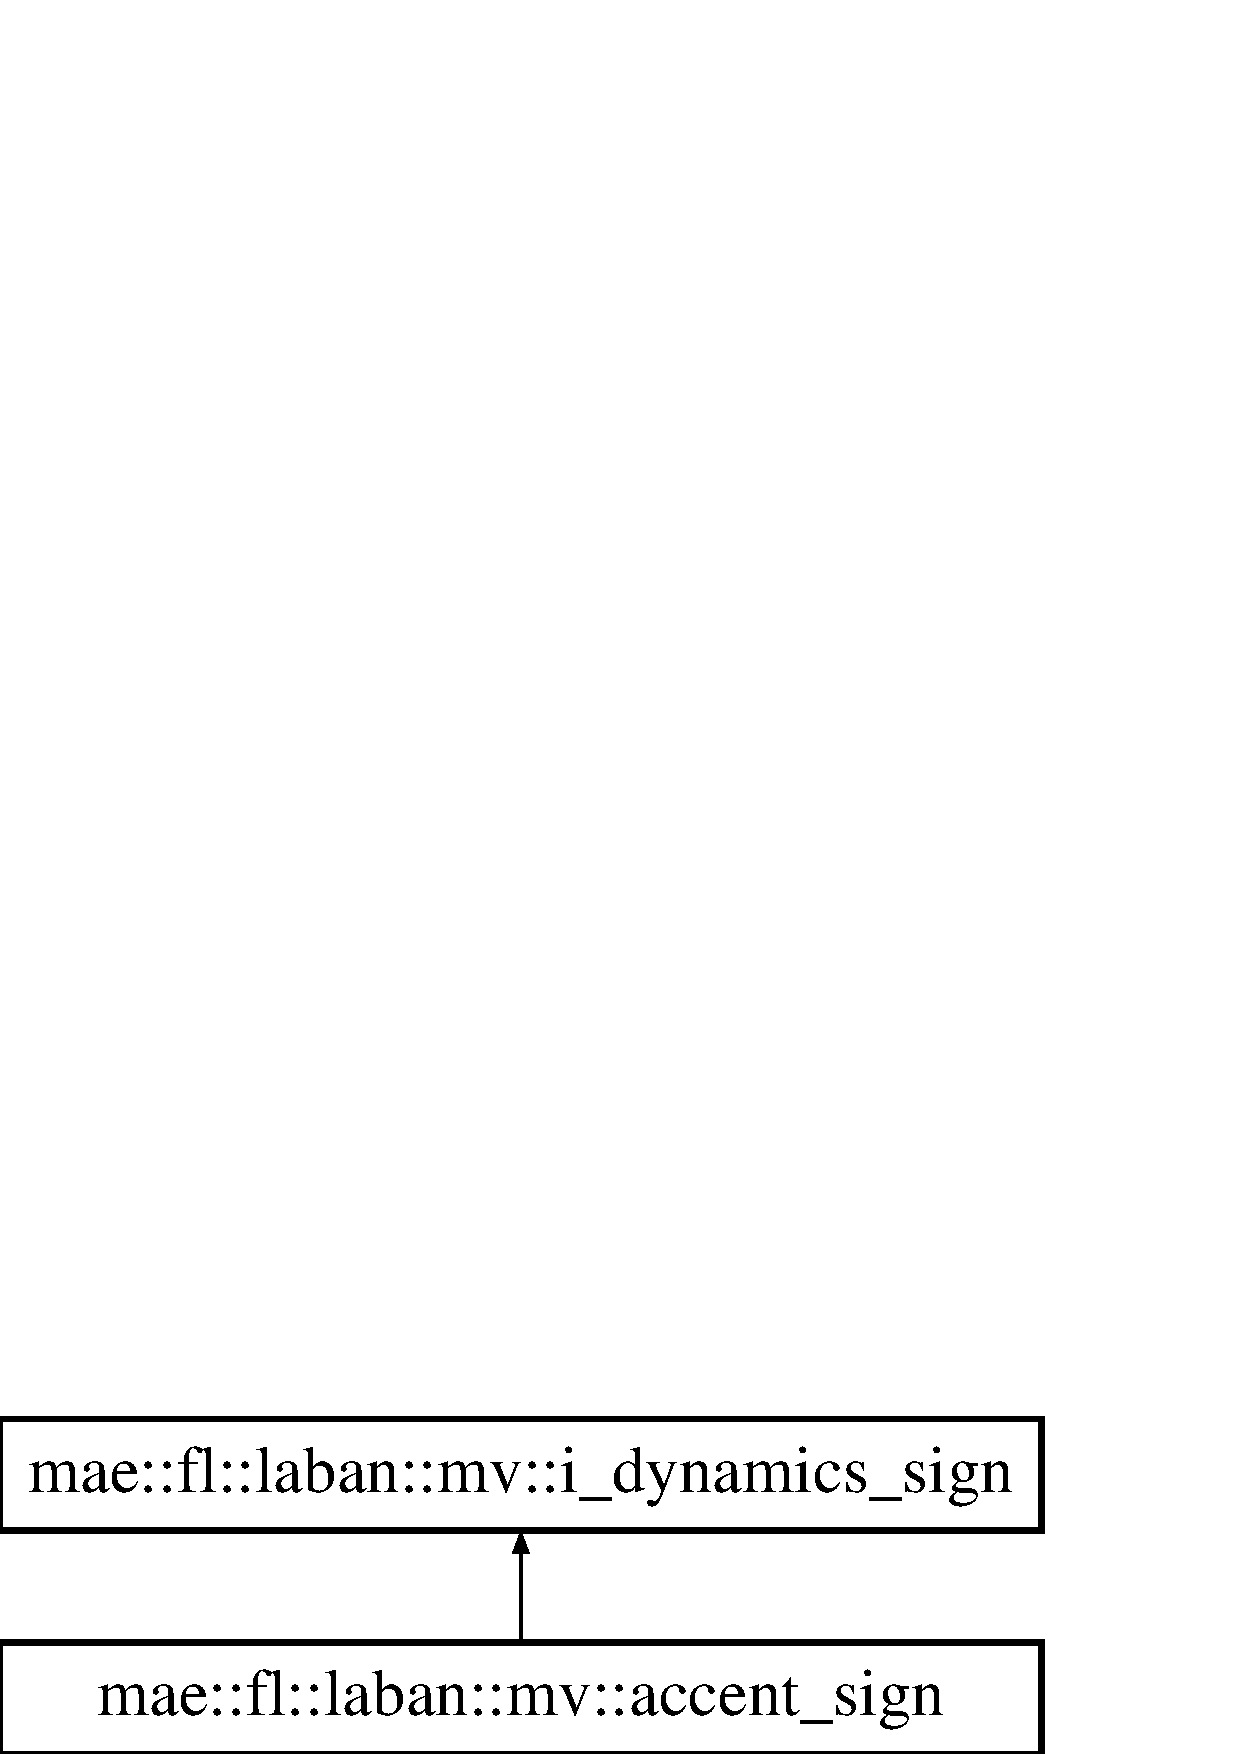
\includegraphics[height=2.000000cm]{classmae_1_1fl_1_1laban_1_1mv_1_1accent__sign}
\end{center}
\end{figure}
\subsection*{Public Member Functions}
\begin{DoxyCompactItemize}
\item 
\hyperlink{classmae_1_1fl_1_1laban_1_1mv_1_1accent__sign_ad025f5ad88ce312168eb134467157892}{accent\-\_\-sign} (unsigned int accent)
\item 
unsigned int \hyperlink{classmae_1_1fl_1_1laban_1_1mv_1_1accent__sign_a2b1b508f59a49d8cc37e910fe1a0c776}{get\-\_\-accent} () const 
\item 
virtual bool \hyperlink{classmae_1_1fl_1_1laban_1_1mv_1_1accent__sign_a891bc39b4718b06ac14243fc17667bd2}{equals} (std\-::shared\-\_\-ptr$<$ \hyperlink{classmae_1_1fl_1_1laban_1_1mv_1_1i__dynamics__sign}{i\-\_\-dynamics\-\_\-sign} $>$ a) const 
\item 
virtual std\-::string \hyperlink{classmae_1_1fl_1_1laban_1_1mv_1_1accent__sign_a018073ffe2b04ce036e64dc5f44943de}{xml} (unsigned int indent=0, std\-::string namesp=\char`\"{}\char`\"{}) const 
\end{DoxyCompactItemize}


\subsection{Constructor \& Destructor Documentation}
\hypertarget{classmae_1_1fl_1_1laban_1_1mv_1_1accent__sign_ad025f5ad88ce312168eb134467157892}{\index{mae\-::fl\-::laban\-::mv\-::accent\-\_\-sign@{mae\-::fl\-::laban\-::mv\-::accent\-\_\-sign}!accent\-\_\-sign@{accent\-\_\-sign}}
\index{accent\-\_\-sign@{accent\-\_\-sign}!mae::fl::laban::mv::accent_sign@{mae\-::fl\-::laban\-::mv\-::accent\-\_\-sign}}
\subsubsection[{accent\-\_\-sign}]{\setlength{\rightskip}{0pt plus 5cm}mae\-::fl\-::laban\-::mv\-::accent\-\_\-sign\-::accent\-\_\-sign (
\begin{DoxyParamCaption}
\item[{unsigned int}]{accent}
\end{DoxyParamCaption}
)}}\label{classmae_1_1fl_1_1laban_1_1mv_1_1accent__sign_ad025f5ad88ce312168eb134467157892}
Creates an accent sign. The accent must be a value between 1 and 5.


\begin{DoxyParams}{Parameters}
{\em accent} & The accent which must be an integer value between 1 and 5. \\
\hline
\end{DoxyParams}


\subsection{Member Function Documentation}
\hypertarget{classmae_1_1fl_1_1laban_1_1mv_1_1accent__sign_a891bc39b4718b06ac14243fc17667bd2}{\index{mae\-::fl\-::laban\-::mv\-::accent\-\_\-sign@{mae\-::fl\-::laban\-::mv\-::accent\-\_\-sign}!equals@{equals}}
\index{equals@{equals}!mae::fl::laban::mv::accent_sign@{mae\-::fl\-::laban\-::mv\-::accent\-\_\-sign}}
\subsubsection[{equals}]{\setlength{\rightskip}{0pt plus 5cm}bool mae\-::fl\-::laban\-::mv\-::accent\-\_\-sign\-::equals (
\begin{DoxyParamCaption}
\item[{std\-::shared\-\_\-ptr$<$ {\bf i\-\_\-dynamics\-\_\-sign} $>$}]{a}
\end{DoxyParamCaption}
) const\hspace{0.3cm}{\ttfamily [virtual]}}}\label{classmae_1_1fl_1_1laban_1_1mv_1_1accent__sign_a891bc39b4718b06ac14243fc17667bd2}
Returns true if signs are equal.


\begin{DoxyParams}{Parameters}
{\em a} & The sign to be compared to. \\
\hline
\end{DoxyParams}
\begin{DoxyReturn}{Returns}
True if equal. 
\end{DoxyReturn}


Implements \hyperlink{classmae_1_1fl_1_1laban_1_1mv_1_1i__dynamics__sign_a8fe9ea5e7b50976e66172042ae01a6e3}{mae\-::fl\-::laban\-::mv\-::i\-\_\-dynamics\-\_\-sign}.

\hypertarget{classmae_1_1fl_1_1laban_1_1mv_1_1accent__sign_a2b1b508f59a49d8cc37e910fe1a0c776}{\index{mae\-::fl\-::laban\-::mv\-::accent\-\_\-sign@{mae\-::fl\-::laban\-::mv\-::accent\-\_\-sign}!get\-\_\-accent@{get\-\_\-accent}}
\index{get\-\_\-accent@{get\-\_\-accent}!mae::fl::laban::mv::accent_sign@{mae\-::fl\-::laban\-::mv\-::accent\-\_\-sign}}
\subsubsection[{get\-\_\-accent}]{\setlength{\rightskip}{0pt plus 5cm}unsigned int mae\-::fl\-::laban\-::mv\-::accent\-\_\-sign\-::get\-\_\-accent (
\begin{DoxyParamCaption}
{}
\end{DoxyParamCaption}
) const}}\label{classmae_1_1fl_1_1laban_1_1mv_1_1accent__sign_a2b1b508f59a49d8cc37e910fe1a0c776}
Returns the accent. \begin{DoxyReturn}{Returns}

\end{DoxyReturn}
\hypertarget{classmae_1_1fl_1_1laban_1_1mv_1_1accent__sign_a018073ffe2b04ce036e64dc5f44943de}{\index{mae\-::fl\-::laban\-::mv\-::accent\-\_\-sign@{mae\-::fl\-::laban\-::mv\-::accent\-\_\-sign}!xml@{xml}}
\index{xml@{xml}!mae::fl::laban::mv::accent_sign@{mae\-::fl\-::laban\-::mv\-::accent\-\_\-sign}}
\subsubsection[{xml}]{\setlength{\rightskip}{0pt plus 5cm}std\-::string mae\-::fl\-::laban\-::mv\-::accent\-\_\-sign\-::xml (
\begin{DoxyParamCaption}
\item[{unsigned int}]{indent = {\ttfamily 0}, }
\item[{std\-::string}]{namesp = {\ttfamily \char`\"{}\char`\"{}}}
\end{DoxyParamCaption}
) const\hspace{0.3cm}{\ttfamily [virtual]}}}\label{classmae_1_1fl_1_1laban_1_1mv_1_1accent__sign_a018073ffe2b04ce036e64dc5f44943de}
Returns the X\-M\-L representation for this element.


\begin{DoxyParams}{Parameters}
{\em indent} & The applied indent. \\
\hline
{\em namesp} & The prefixed X\-M\-L namespace.\\
\hline
\end{DoxyParams}
\begin{DoxyReturn}{Returns}
The X\-M\-L string. 
\end{DoxyReturn}


Implements \hyperlink{classmae_1_1fl_1_1laban_1_1mv_1_1i__dynamics__sign_aa6332ee3990c3b59fbe8035aeae84503}{mae\-::fl\-::laban\-::mv\-::i\-\_\-dynamics\-\_\-sign}.



The documentation for this class was generated from the following files\-:\begin{DoxyCompactItemize}
\item 
src/mae/fl/laban/mv/accent\-\_\-sign.\-hpp\item 
src/mae/fl/laban/mv/accent\-\_\-sign.\-cpp\end{DoxyCompactItemize}

\hypertarget{classmae_1_1fl_1_1angular__joint}{\section{mae\-:\-:fl\-:\-:angular\-\_\-joint Class Reference}
\label{classmae_1_1fl_1_1angular__joint}\index{mae\-::fl\-::angular\-\_\-joint@{mae\-::fl\-::angular\-\_\-joint}}
}
\subsection*{Public Member Functions}
\begin{DoxyCompactItemize}
\item 
\hyperlink{classmae_1_1fl_1_1angular__joint_a22ba6c973e1e3c0c91b8d48948529182}{angular\-\_\-joint} ()
\item 
\hyperlink{classmae_1_1fl_1_1angular__joint_a100bba0dfbbe4a0d9bff62a3d3831934}{angular\-\_\-joint} (double phi, double theta, double confidence=1.\-0)
\item 
virtual void \hyperlink{classmae_1_1fl_1_1angular__joint_ad0df6abcd02ebd7f536fcb0936a359d0}{set\-\_\-phi} (double x)
\item 
virtual double \hyperlink{classmae_1_1fl_1_1angular__joint_a780ff68cff4e673b31c0ccdcead81440}{get\-\_\-phi} () const 
\item 
virtual void \hyperlink{classmae_1_1fl_1_1angular__joint_abf699155f7efa2c2b0052f064e8efacc}{set\-\_\-theta} (double x)
\item 
virtual double \hyperlink{classmae_1_1fl_1_1angular__joint_a5452def9f039c981b553ae7783dbf4c7}{get\-\_\-theta} () const 
\item 
virtual void \hyperlink{classmae_1_1fl_1_1angular__joint_ae4a858f782f3af9ba88a4f3b9fb29317}{set\-\_\-valid} (bool is\-Valid)
\item 
virtual bool \hyperlink{classmae_1_1fl_1_1angular__joint_a5235990dd2181368ad716172c348a663}{is\-\_\-valid} () const 
\item 
virtual void \hyperlink{classmae_1_1fl_1_1angular__joint_a4ae61fdcaa4746d56a32f14a51ebfa37}{set\-\_\-confidence} (double confidence)
\item 
virtual double \hyperlink{classmae_1_1fl_1_1angular__joint_a2b9aea9baff5d9dcb56aa8b0be1a7d59}{get\-\_\-confidence} () const 
\end{DoxyCompactItemize}
\subsection*{Friends}
\begin{DoxyCompactItemize}
\item 
\hypertarget{classmae_1_1fl_1_1angular__joint_adec3d68c1b5e4c0a50f6887a23fbf3ab}{std\-::ostream \& {\bfseries operator$<$$<$} (std\-::ostream \&os, const \hyperlink{classmae_1_1fl_1_1angular__joint}{angular\-\_\-joint} \&obj)}\label{classmae_1_1fl_1_1angular__joint_adec3d68c1b5e4c0a50f6887a23fbf3ab}

\item 
\hypertarget{classmae_1_1fl_1_1angular__joint_a3d57ca1c56c0804d2b07874dedac505c}{std\-::ostream \& {\bfseries operator$<$$<$} (std\-::ostream \&os, const std\-::shared\-\_\-ptr$<$ \hyperlink{classmae_1_1fl_1_1angular__joint}{angular\-\_\-joint} $>$ \&obj)}\label{classmae_1_1fl_1_1angular__joint_a3d57ca1c56c0804d2b07874dedac505c}

\end{DoxyCompactItemize}


\subsection{Constructor \& Destructor Documentation}
\hypertarget{classmae_1_1fl_1_1angular__joint_a22ba6c973e1e3c0c91b8d48948529182}{\index{mae\-::fl\-::angular\-\_\-joint@{mae\-::fl\-::angular\-\_\-joint}!angular\-\_\-joint@{angular\-\_\-joint}}
\index{angular\-\_\-joint@{angular\-\_\-joint}!mae::fl::angular_joint@{mae\-::fl\-::angular\-\_\-joint}}
\subsubsection[{angular\-\_\-joint}]{\setlength{\rightskip}{0pt plus 5cm}mae\-::fl\-::angular\-\_\-joint\-::angular\-\_\-joint (
\begin{DoxyParamCaption}
{}
\end{DoxyParamCaption}
)}}\label{classmae_1_1fl_1_1angular__joint_a22ba6c973e1e3c0c91b8d48948529182}
Creates a new invalid joint. \hypertarget{classmae_1_1fl_1_1angular__joint_a100bba0dfbbe4a0d9bff62a3d3831934}{\index{mae\-::fl\-::angular\-\_\-joint@{mae\-::fl\-::angular\-\_\-joint}!angular\-\_\-joint@{angular\-\_\-joint}}
\index{angular\-\_\-joint@{angular\-\_\-joint}!mae::fl::angular_joint@{mae\-::fl\-::angular\-\_\-joint}}
\subsubsection[{angular\-\_\-joint}]{\setlength{\rightskip}{0pt plus 5cm}mae\-::fl\-::angular\-\_\-joint\-::angular\-\_\-joint (
\begin{DoxyParamCaption}
\item[{double}]{phi, }
\item[{double}]{theta, }
\item[{double}]{confidence = {\ttfamily 1.0}}
\end{DoxyParamCaption}
)}}\label{classmae_1_1fl_1_1angular__joint_a100bba0dfbbe4a0d9bff62a3d3831934}
Creates a new joint with the values set.


\begin{DoxyParams}{Parameters}
{\em phi} & The elevation phi. \\
\hline
{\em theta} & The azimuth theta. \\
\hline
{\em confidence} & The confidence (a value between zero and one, where one is the most confident). \\
\hline
\end{DoxyParams}


\subsection{Member Function Documentation}
\hypertarget{classmae_1_1fl_1_1angular__joint_a2b9aea9baff5d9dcb56aa8b0be1a7d59}{\index{mae\-::fl\-::angular\-\_\-joint@{mae\-::fl\-::angular\-\_\-joint}!get\-\_\-confidence@{get\-\_\-confidence}}
\index{get\-\_\-confidence@{get\-\_\-confidence}!mae::fl::angular_joint@{mae\-::fl\-::angular\-\_\-joint}}
\subsubsection[{get\-\_\-confidence}]{\setlength{\rightskip}{0pt plus 5cm}double mae\-::fl\-::angular\-\_\-joint\-::get\-\_\-confidence (
\begin{DoxyParamCaption}
{}
\end{DoxyParamCaption}
) const\hspace{0.3cm}{\ttfamily [virtual]}}}\label{classmae_1_1fl_1_1angular__joint_a2b9aea9baff5d9dcb56aa8b0be1a7d59}
Returns the confidence for this joint which is a value between zero and one, where one is the most confident. \hypertarget{classmae_1_1fl_1_1angular__joint_a780ff68cff4e673b31c0ccdcead81440}{\index{mae\-::fl\-::angular\-\_\-joint@{mae\-::fl\-::angular\-\_\-joint}!get\-\_\-phi@{get\-\_\-phi}}
\index{get\-\_\-phi@{get\-\_\-phi}!mae::fl::angular_joint@{mae\-::fl\-::angular\-\_\-joint}}
\subsubsection[{get\-\_\-phi}]{\setlength{\rightskip}{0pt plus 5cm}double mae\-::fl\-::angular\-\_\-joint\-::get\-\_\-phi (
\begin{DoxyParamCaption}
{}
\end{DoxyParamCaption}
) const\hspace{0.3cm}{\ttfamily [virtual]}}}\label{classmae_1_1fl_1_1angular__joint_a780ff68cff4e673b31c0ccdcead81440}
Returns the value for phi.

\begin{DoxyReturn}{Returns}
The value. 
\end{DoxyReturn}
\hypertarget{classmae_1_1fl_1_1angular__joint_a5452def9f039c981b553ae7783dbf4c7}{\index{mae\-::fl\-::angular\-\_\-joint@{mae\-::fl\-::angular\-\_\-joint}!get\-\_\-theta@{get\-\_\-theta}}
\index{get\-\_\-theta@{get\-\_\-theta}!mae::fl::angular_joint@{mae\-::fl\-::angular\-\_\-joint}}
\subsubsection[{get\-\_\-theta}]{\setlength{\rightskip}{0pt plus 5cm}double mae\-::fl\-::angular\-\_\-joint\-::get\-\_\-theta (
\begin{DoxyParamCaption}
{}
\end{DoxyParamCaption}
) const\hspace{0.3cm}{\ttfamily [virtual]}}}\label{classmae_1_1fl_1_1angular__joint_a5452def9f039c981b553ae7783dbf4c7}
Returns the value for theta.

\begin{DoxyReturn}{Returns}
The value. 
\end{DoxyReturn}
\hypertarget{classmae_1_1fl_1_1angular__joint_a5235990dd2181368ad716172c348a663}{\index{mae\-::fl\-::angular\-\_\-joint@{mae\-::fl\-::angular\-\_\-joint}!is\-\_\-valid@{is\-\_\-valid}}
\index{is\-\_\-valid@{is\-\_\-valid}!mae::fl::angular_joint@{mae\-::fl\-::angular\-\_\-joint}}
\subsubsection[{is\-\_\-valid}]{\setlength{\rightskip}{0pt plus 5cm}bool mae\-::fl\-::angular\-\_\-joint\-::is\-\_\-valid (
\begin{DoxyParamCaption}
{}
\end{DoxyParamCaption}
) const\hspace{0.3cm}{\ttfamily [virtual]}}}\label{classmae_1_1fl_1_1angular__joint_a5235990dd2181368ad716172c348a663}
Returns the validity of this joint.

\begin{DoxyReturn}{Returns}
True if valid. 
\end{DoxyReturn}
\hypertarget{classmae_1_1fl_1_1angular__joint_a4ae61fdcaa4746d56a32f14a51ebfa37}{\index{mae\-::fl\-::angular\-\_\-joint@{mae\-::fl\-::angular\-\_\-joint}!set\-\_\-confidence@{set\-\_\-confidence}}
\index{set\-\_\-confidence@{set\-\_\-confidence}!mae::fl::angular_joint@{mae\-::fl\-::angular\-\_\-joint}}
\subsubsection[{set\-\_\-confidence}]{\setlength{\rightskip}{0pt plus 5cm}void mae\-::fl\-::angular\-\_\-joint\-::set\-\_\-confidence (
\begin{DoxyParamCaption}
\item[{double}]{confidence}
\end{DoxyParamCaption}
)\hspace{0.3cm}{\ttfamily [virtual]}}}\label{classmae_1_1fl_1_1angular__joint_a4ae61fdcaa4746d56a32f14a51ebfa37}
Sets the confidence for this joint which is a value between zero and one, where one is the most confident.


\begin{DoxyParams}{Parameters}
{\em confidence} & The confidence. \\
\hline
\end{DoxyParams}
\hypertarget{classmae_1_1fl_1_1angular__joint_ad0df6abcd02ebd7f536fcb0936a359d0}{\index{mae\-::fl\-::angular\-\_\-joint@{mae\-::fl\-::angular\-\_\-joint}!set\-\_\-phi@{set\-\_\-phi}}
\index{set\-\_\-phi@{set\-\_\-phi}!mae::fl::angular_joint@{mae\-::fl\-::angular\-\_\-joint}}
\subsubsection[{set\-\_\-phi}]{\setlength{\rightskip}{0pt plus 5cm}void mae\-::fl\-::angular\-\_\-joint\-::set\-\_\-phi (
\begin{DoxyParamCaption}
\item[{double}]{x}
\end{DoxyParamCaption}
)\hspace{0.3cm}{\ttfamily [virtual]}}}\label{classmae_1_1fl_1_1angular__joint_ad0df6abcd02ebd7f536fcb0936a359d0}
Sets the value for phi.


\begin{DoxyParams}{Parameters}
{\em x} & The value. \\
\hline
\end{DoxyParams}
\hypertarget{classmae_1_1fl_1_1angular__joint_abf699155f7efa2c2b0052f064e8efacc}{\index{mae\-::fl\-::angular\-\_\-joint@{mae\-::fl\-::angular\-\_\-joint}!set\-\_\-theta@{set\-\_\-theta}}
\index{set\-\_\-theta@{set\-\_\-theta}!mae::fl::angular_joint@{mae\-::fl\-::angular\-\_\-joint}}
\subsubsection[{set\-\_\-theta}]{\setlength{\rightskip}{0pt plus 5cm}void mae\-::fl\-::angular\-\_\-joint\-::set\-\_\-theta (
\begin{DoxyParamCaption}
\item[{double}]{x}
\end{DoxyParamCaption}
)\hspace{0.3cm}{\ttfamily [virtual]}}}\label{classmae_1_1fl_1_1angular__joint_abf699155f7efa2c2b0052f064e8efacc}
Sets the value for theta.


\begin{DoxyParams}{Parameters}
{\em x} & The value. \\
\hline
\end{DoxyParams}
\hypertarget{classmae_1_1fl_1_1angular__joint_ae4a858f782f3af9ba88a4f3b9fb29317}{\index{mae\-::fl\-::angular\-\_\-joint@{mae\-::fl\-::angular\-\_\-joint}!set\-\_\-valid@{set\-\_\-valid}}
\index{set\-\_\-valid@{set\-\_\-valid}!mae::fl::angular_joint@{mae\-::fl\-::angular\-\_\-joint}}
\subsubsection[{set\-\_\-valid}]{\setlength{\rightskip}{0pt plus 5cm}void mae\-::fl\-::angular\-\_\-joint\-::set\-\_\-valid (
\begin{DoxyParamCaption}
\item[{bool}]{is\-Valid}
\end{DoxyParamCaption}
)\hspace{0.3cm}{\ttfamily [virtual]}}}\label{classmae_1_1fl_1_1angular__joint_ae4a858f782f3af9ba88a4f3b9fb29317}
Sets the validity of this joint.


\begin{DoxyParams}{Parameters}
{\em is\-Valid} & The validity. \\
\hline
\end{DoxyParams}


The documentation for this class was generated from the following files\-:\begin{DoxyCompactItemize}
\item 
src/mae/fl/angular\-\_\-joint.\-hpp\item 
src/mae/fl/angular\-\_\-joint.\-cpp\end{DoxyCompactItemize}

\hypertarget{classmae_1_1fl_1_1angular__skeleton}{\section{mae\-:\-:fl\-:\-:angular\-\_\-skeleton Class Reference}
\label{classmae_1_1fl_1_1angular__skeleton}\index{mae\-::fl\-::angular\-\_\-skeleton@{mae\-::fl\-::angular\-\_\-skeleton}}
}
\subsection*{Public Member Functions}
\begin{DoxyCompactItemize}
\item 
\hyperlink{classmae_1_1fl_1_1angular__skeleton_a5b9dcc5e7582bdca3d18f14eec629156}{angular\-\_\-skeleton} ()
\item 
virtual void \hyperlink{classmae_1_1fl_1_1angular__skeleton_aa44853baa4576d65a2a1699d2ca10eff}{set\-\_\-joint} (int body\-\_\-part, std\-::shared\-\_\-ptr$<$ \hyperlink{classmae_1_1fl_1_1angular__joint}{angular\-\_\-joint} $>$ joint)
\item 
virtual std\-::shared\-\_\-ptr\\*
$<$ \hyperlink{classmae_1_1fl_1_1angular__joint}{angular\-\_\-joint} $>$ \hyperlink{classmae_1_1fl_1_1angular__skeleton_ad8bd5bc24f4764df37ec334dc236c2a1}{get\-\_\-joint} (int body\-\_\-part) const 
\item 
virtual std\-::shared\-\_\-ptr\\*
$<$ \hyperlink{classmae_1_1hierarchy}{hierarchy} $>$ \hyperlink{classmae_1_1fl_1_1angular__skeleton_a5ce839e030dc0359334e8ba337401417}{get\-\_\-hierarchy} () const 
\item 
virtual void \hyperlink{classmae_1_1fl_1_1angular__skeleton_a4b3d02d386a84c89ba9bb9409a5aa173}{set\-\_\-hierarchy} (std\-::shared\-\_\-ptr$<$ \hyperlink{classmae_1_1hierarchy}{hierarchy} $>$ \hyperlink{classmae_1_1hierarchy}{hierarchy})
\item 
virtual void \hyperlink{classmae_1_1fl_1_1angular__skeleton_a9f1c654e0bf6aab498eeb623656fdf1b}{set\-\_\-torso\-\_\-basis} (std\-::shared\-\_\-ptr$<$ \hyperlink{classmae_1_1math_1_1basis}{mae\-::math\-::basis} $>$ torso\-\_\-basis)
\item 
virtual std\-::shared\-\_\-ptr\\*
$<$ \hyperlink{classmae_1_1math_1_1basis}{mae\-::math\-::basis} $>$ \hyperlink{classmae_1_1fl_1_1angular__skeleton_a752ce57c7aacc53dfdfab0b096fc8e17}{get\-\_\-torso\-\_\-basis} () const 
\item 
virtual void \hyperlink{classmae_1_1fl_1_1angular__skeleton_ac869c6b0a431f2f3810d319e47986069}{set\-\_\-top\-\_\-down} (std\-::shared\-\_\-ptr$<$ \hyperlink{classmae_1_1bone}{bone} $>$ top\-\_\-down)
\item 
virtual std\-::shared\-\_\-ptr$<$ \hyperlink{classmae_1_1bone}{bone} $>$ \hyperlink{classmae_1_1fl_1_1angular__skeleton_a138779503a2ab02bad8d15705adf3203}{get\-\_\-top\-\_\-down} () const 
\item 
virtual void \hyperlink{classmae_1_1fl_1_1angular__skeleton_a13eb821e9c93c218e4d34a9c02960ebc}{set\-\_\-right\-\_\-left} (std\-::shared\-\_\-ptr$<$ \hyperlink{classmae_1_1bone}{bone} $>$ right\-\_\-left)
\item 
virtual std\-::shared\-\_\-ptr$<$ \hyperlink{classmae_1_1bone}{bone} $>$ \hyperlink{classmae_1_1fl_1_1angular__skeleton_ae91ef0dd87f4ed99c144fbcfadc59559}{get\-\_\-right\-\_\-left} () const 
\item 
virtual void \hyperlink{classmae_1_1fl_1_1angular__skeleton_a682bb661d0451ada678a49d5bfbab72e}{set\-\_\-weight} (std\-::shared\-\_\-ptr$<$ \hyperlink{classmae_1_1math_1_1vec3d}{mae\-::math\-::vec3d} $>$ weight)
\item 
virtual std\-::shared\-\_\-ptr\\*
$<$ \hyperlink{classmae_1_1math_1_1vec3d}{mae\-::math\-::vec3d} $>$ \hyperlink{classmae_1_1fl_1_1angular__skeleton_a07633f191e91165035aeaacfcb553130}{get\-\_\-weight} () const 
\item 
virtual std\-::string \hyperlink{classmae_1_1fl_1_1angular__skeleton_a786a62157d68c11a223ab22755a6d326}{str} () const 
\end{DoxyCompactItemize}
\subsection*{Friends}
\begin{DoxyCompactItemize}
\item 
std\-::ostream \& \hyperlink{classmae_1_1fl_1_1angular__skeleton_a34e41467f6fcab05252e8e28b2cbdd3e}{operator$<$$<$} (std\-::ostream \&os, const std\-::shared\-\_\-ptr$<$ \hyperlink{classmae_1_1fl_1_1angular__skeleton}{angular\-\_\-skeleton} $>$ \&obj)
\end{DoxyCompactItemize}


\subsection{Constructor \& Destructor Documentation}
\hypertarget{classmae_1_1fl_1_1angular__skeleton_a5b9dcc5e7582bdca3d18f14eec629156}{\index{mae\-::fl\-::angular\-\_\-skeleton@{mae\-::fl\-::angular\-\_\-skeleton}!angular\-\_\-skeleton@{angular\-\_\-skeleton}}
\index{angular\-\_\-skeleton@{angular\-\_\-skeleton}!mae::fl::angular_skeleton@{mae\-::fl\-::angular\-\_\-skeleton}}
\subsubsection[{angular\-\_\-skeleton}]{\setlength{\rightskip}{0pt plus 5cm}mae\-::fl\-::angular\-\_\-skeleton\-::angular\-\_\-skeleton (
\begin{DoxyParamCaption}
{}
\end{DoxyParamCaption}
)}}\label{classmae_1_1fl_1_1angular__skeleton_a5b9dcc5e7582bdca3d18f14eec629156}
Creates a new angular skeleton with the joints represented by two angles T\-H\-E\-T\-A and P\-H\-I. 

\subsection{Member Function Documentation}
\hypertarget{classmae_1_1fl_1_1angular__skeleton_a5ce839e030dc0359334e8ba337401417}{\index{mae\-::fl\-::angular\-\_\-skeleton@{mae\-::fl\-::angular\-\_\-skeleton}!get\-\_\-hierarchy@{get\-\_\-hierarchy}}
\index{get\-\_\-hierarchy@{get\-\_\-hierarchy}!mae::fl::angular_skeleton@{mae\-::fl\-::angular\-\_\-skeleton}}
\subsubsection[{get\-\_\-hierarchy}]{\setlength{\rightskip}{0pt plus 5cm}std\-::shared\-\_\-ptr$<$ {\bf hierarchy} $>$ mae\-::fl\-::angular\-\_\-skeleton\-::get\-\_\-hierarchy (
\begin{DoxyParamCaption}
{}
\end{DoxyParamCaption}
) const\hspace{0.3cm}{\ttfamily [virtual]}}}\label{classmae_1_1fl_1_1angular__skeleton_a5ce839e030dc0359334e8ba337401417}
Returns a shared pointer to the used hierarchy. If not hierarchy is set, a default hierarchy is assumed. \begin{DoxyReturn}{Returns}
A shared pointer to the hierarchy. 
\end{DoxyReturn}
\hypertarget{classmae_1_1fl_1_1angular__skeleton_ad8bd5bc24f4764df37ec334dc236c2a1}{\index{mae\-::fl\-::angular\-\_\-skeleton@{mae\-::fl\-::angular\-\_\-skeleton}!get\-\_\-joint@{get\-\_\-joint}}
\index{get\-\_\-joint@{get\-\_\-joint}!mae::fl::angular_skeleton@{mae\-::fl\-::angular\-\_\-skeleton}}
\subsubsection[{get\-\_\-joint}]{\setlength{\rightskip}{0pt plus 5cm}std\-::shared\-\_\-ptr$<$ {\bf angular\-\_\-joint} $>$ mae\-::fl\-::angular\-\_\-skeleton\-::get\-\_\-joint (
\begin{DoxyParamCaption}
\item[{int}]{body\-\_\-part}
\end{DoxyParamCaption}
) const\hspace{0.3cm}{\ttfamily [virtual]}}}\label{classmae_1_1fl_1_1angular__skeleton_ad8bd5bc24f4764df37ec334dc236c2a1}
Returns an angular joint.


\begin{DoxyParams}{Parameters}
{\em body\-\_\-part} & The addressed body part. \\
\hline
\end{DoxyParams}
\begin{DoxyReturn}{Returns}
A shared pointer to the joint. 
\end{DoxyReturn}
\hypertarget{classmae_1_1fl_1_1angular__skeleton_ae91ef0dd87f4ed99c144fbcfadc59559}{\index{mae\-::fl\-::angular\-\_\-skeleton@{mae\-::fl\-::angular\-\_\-skeleton}!get\-\_\-right\-\_\-left@{get\-\_\-right\-\_\-left}}
\index{get\-\_\-right\-\_\-left@{get\-\_\-right\-\_\-left}!mae::fl::angular_skeleton@{mae\-::fl\-::angular\-\_\-skeleton}}
\subsubsection[{get\-\_\-right\-\_\-left}]{\setlength{\rightskip}{0pt plus 5cm}std\-::shared\-\_\-ptr$<$ {\bf bone} $>$ mae\-::fl\-::angular\-\_\-skeleton\-::get\-\_\-right\-\_\-left (
\begin{DoxyParamCaption}
{}
\end{DoxyParamCaption}
) const\hspace{0.3cm}{\ttfamily [virtual]}}}\label{classmae_1_1fl_1_1angular__skeleton_ae91ef0dd87f4ed99c144fbcfadc59559}
Returns the right-\/left direction of this skeleton by giving a bone. The bone ranges from one torso joint to another.


\begin{DoxyParams}{Parameters}
{\em top\-\_\-down} & A shared pointer to the bone. \\
\hline
\end{DoxyParams}
\hypertarget{classmae_1_1fl_1_1angular__skeleton_a138779503a2ab02bad8d15705adf3203}{\index{mae\-::fl\-::angular\-\_\-skeleton@{mae\-::fl\-::angular\-\_\-skeleton}!get\-\_\-top\-\_\-down@{get\-\_\-top\-\_\-down}}
\index{get\-\_\-top\-\_\-down@{get\-\_\-top\-\_\-down}!mae::fl::angular_skeleton@{mae\-::fl\-::angular\-\_\-skeleton}}
\subsubsection[{get\-\_\-top\-\_\-down}]{\setlength{\rightskip}{0pt plus 5cm}std\-::shared\-\_\-ptr$<$ {\bf bone} $>$ mae\-::fl\-::angular\-\_\-skeleton\-::get\-\_\-top\-\_\-down (
\begin{DoxyParamCaption}
{}
\end{DoxyParamCaption}
) const\hspace{0.3cm}{\ttfamily [virtual]}}}\label{classmae_1_1fl_1_1angular__skeleton_a138779503a2ab02bad8d15705adf3203}
Returns the top-\/down direction of this skeleton by giving a bone. The bone ranges from one torso joint to another.


\begin{DoxyParams}{Parameters}
{\em top\-\_\-down} & A shared pointer to the bone. \\
\hline
\end{DoxyParams}
\hypertarget{classmae_1_1fl_1_1angular__skeleton_a752ce57c7aacc53dfdfab0b096fc8e17}{\index{mae\-::fl\-::angular\-\_\-skeleton@{mae\-::fl\-::angular\-\_\-skeleton}!get\-\_\-torso\-\_\-basis@{get\-\_\-torso\-\_\-basis}}
\index{get\-\_\-torso\-\_\-basis@{get\-\_\-torso\-\_\-basis}!mae::fl::angular_skeleton@{mae\-::fl\-::angular\-\_\-skeleton}}
\subsubsection[{get\-\_\-torso\-\_\-basis}]{\setlength{\rightskip}{0pt plus 5cm}std\-::shared\-\_\-ptr$<$ {\bf mae\-::math\-::basis} $>$ mae\-::fl\-::angular\-\_\-skeleton\-::get\-\_\-torso\-\_\-basis (
\begin{DoxyParamCaption}
{}
\end{DoxyParamCaption}
) const\hspace{0.3cm}{\ttfamily [virtual]}}}\label{classmae_1_1fl_1_1angular__skeleton_a752ce57c7aacc53dfdfab0b096fc8e17}
Returns the torso basis.

The directions are\-: u The top-\/down or weight direction. r The right-\/left direction. t The direction standing on u and r (pointing from torso to the front).

\begin{DoxyReturn}{Returns}
The torso basis. 
\end{DoxyReturn}
\hypertarget{classmae_1_1fl_1_1angular__skeleton_a07633f191e91165035aeaacfcb553130}{\index{mae\-::fl\-::angular\-\_\-skeleton@{mae\-::fl\-::angular\-\_\-skeleton}!get\-\_\-weight@{get\-\_\-weight}}
\index{get\-\_\-weight@{get\-\_\-weight}!mae::fl::angular_skeleton@{mae\-::fl\-::angular\-\_\-skeleton}}
\subsubsection[{get\-\_\-weight}]{\setlength{\rightskip}{0pt plus 5cm}std\-::shared\-\_\-ptr$<$ {\bf mae\-::math\-::vec3d} $>$ mae\-::fl\-::angular\-\_\-skeleton\-::get\-\_\-weight (
\begin{DoxyParamCaption}
{}
\end{DoxyParamCaption}
) const\hspace{0.3cm}{\ttfamily [virtual]}}}\label{classmae_1_1fl_1_1angular__skeleton_a07633f191e91165035aeaacfcb553130}
Returns the weight vector for this skeleton. If none is set, a null pointer will be returned.

\begin{DoxyReturn}{Returns}
The weight or null. 
\end{DoxyReturn}
\hypertarget{classmae_1_1fl_1_1angular__skeleton_a4b3d02d386a84c89ba9bb9409a5aa173}{\index{mae\-::fl\-::angular\-\_\-skeleton@{mae\-::fl\-::angular\-\_\-skeleton}!set\-\_\-hierarchy@{set\-\_\-hierarchy}}
\index{set\-\_\-hierarchy@{set\-\_\-hierarchy}!mae::fl::angular_skeleton@{mae\-::fl\-::angular\-\_\-skeleton}}
\subsubsection[{set\-\_\-hierarchy}]{\setlength{\rightskip}{0pt plus 5cm}void mae\-::fl\-::angular\-\_\-skeleton\-::set\-\_\-hierarchy (
\begin{DoxyParamCaption}
\item[{std\-::shared\-\_\-ptr$<$ {\bf hierarchy} $>$}]{hierarchy}
\end{DoxyParamCaption}
)\hspace{0.3cm}{\ttfamily [virtual]}}}\label{classmae_1_1fl_1_1angular__skeleton_a4b3d02d386a84c89ba9bb9409a5aa173}
Sets the hierarchy 
\begin{DoxyParams}{Parameters}
{\em hierarchy} & A smart pointer to the hierarchy. \\
\hline
\end{DoxyParams}
\hypertarget{classmae_1_1fl_1_1angular__skeleton_aa44853baa4576d65a2a1699d2ca10eff}{\index{mae\-::fl\-::angular\-\_\-skeleton@{mae\-::fl\-::angular\-\_\-skeleton}!set\-\_\-joint@{set\-\_\-joint}}
\index{set\-\_\-joint@{set\-\_\-joint}!mae::fl::angular_skeleton@{mae\-::fl\-::angular\-\_\-skeleton}}
\subsubsection[{set\-\_\-joint}]{\setlength{\rightskip}{0pt plus 5cm}void mae\-::fl\-::angular\-\_\-skeleton\-::set\-\_\-joint (
\begin{DoxyParamCaption}
\item[{int}]{body\-\_\-part, }
\item[{std\-::shared\-\_\-ptr$<$ {\bf angular\-\_\-joint} $>$}]{joint}
\end{DoxyParamCaption}
)\hspace{0.3cm}{\ttfamily [virtual]}}}\label{classmae_1_1fl_1_1angular__skeleton_aa44853baa4576d65a2a1699d2ca10eff}
Sets an angular joint.


\begin{DoxyParams}{Parameters}
{\em body\-\_\-part} & The addresses body part. \\
\hline
{\em joint} & A shared pointer to the joint. \\
\hline
\end{DoxyParams}
\hypertarget{classmae_1_1fl_1_1angular__skeleton_a13eb821e9c93c218e4d34a9c02960ebc}{\index{mae\-::fl\-::angular\-\_\-skeleton@{mae\-::fl\-::angular\-\_\-skeleton}!set\-\_\-right\-\_\-left@{set\-\_\-right\-\_\-left}}
\index{set\-\_\-right\-\_\-left@{set\-\_\-right\-\_\-left}!mae::fl::angular_skeleton@{mae\-::fl\-::angular\-\_\-skeleton}}
\subsubsection[{set\-\_\-right\-\_\-left}]{\setlength{\rightskip}{0pt plus 5cm}void mae\-::fl\-::angular\-\_\-skeleton\-::set\-\_\-right\-\_\-left (
\begin{DoxyParamCaption}
\item[{std\-::shared\-\_\-ptr$<$ {\bf bone} $>$}]{right\-\_\-left}
\end{DoxyParamCaption}
)\hspace{0.3cm}{\ttfamily [virtual]}}}\label{classmae_1_1fl_1_1angular__skeleton_a13eb821e9c93c218e4d34a9c02960ebc}
Sets the right-\/left direction of this skeleton by defining a bone. The bone must range from one torso joint to another and need not to follow the hierarchy (but the id's must be defined).


\begin{DoxyParams}{Parameters}
{\em top\-\_\-down} & A shared pointer to the bone. \\
\hline
\end{DoxyParams}
\hypertarget{classmae_1_1fl_1_1angular__skeleton_ac869c6b0a431f2f3810d319e47986069}{\index{mae\-::fl\-::angular\-\_\-skeleton@{mae\-::fl\-::angular\-\_\-skeleton}!set\-\_\-top\-\_\-down@{set\-\_\-top\-\_\-down}}
\index{set\-\_\-top\-\_\-down@{set\-\_\-top\-\_\-down}!mae::fl::angular_skeleton@{mae\-::fl\-::angular\-\_\-skeleton}}
\subsubsection[{set\-\_\-top\-\_\-down}]{\setlength{\rightskip}{0pt plus 5cm}void mae\-::fl\-::angular\-\_\-skeleton\-::set\-\_\-top\-\_\-down (
\begin{DoxyParamCaption}
\item[{std\-::shared\-\_\-ptr$<$ {\bf bone} $>$}]{top\-\_\-down}
\end{DoxyParamCaption}
)\hspace{0.3cm}{\ttfamily [virtual]}}}\label{classmae_1_1fl_1_1angular__skeleton_ac869c6b0a431f2f3810d319e47986069}
Sets the top-\/down direction of this skeleton by defining a bone. The bone must range from one torso joint to another and need not to follow the hierarchy (but the id's must be defined).


\begin{DoxyParams}{Parameters}
{\em top\-\_\-down} & A shared pointer to the bone. \\
\hline
\end{DoxyParams}
\hypertarget{classmae_1_1fl_1_1angular__skeleton_a9f1c654e0bf6aab498eeb623656fdf1b}{\index{mae\-::fl\-::angular\-\_\-skeleton@{mae\-::fl\-::angular\-\_\-skeleton}!set\-\_\-torso\-\_\-basis@{set\-\_\-torso\-\_\-basis}}
\index{set\-\_\-torso\-\_\-basis@{set\-\_\-torso\-\_\-basis}!mae::fl::angular_skeleton@{mae\-::fl\-::angular\-\_\-skeleton}}
\subsubsection[{set\-\_\-torso\-\_\-basis}]{\setlength{\rightskip}{0pt plus 5cm}void mae\-::fl\-::angular\-\_\-skeleton\-::set\-\_\-torso\-\_\-basis (
\begin{DoxyParamCaption}
\item[{std\-::shared\-\_\-ptr$<$ {\bf mae\-::math\-::basis} $>$}]{torso\-\_\-basis}
\end{DoxyParamCaption}
)\hspace{0.3cm}{\ttfamily [virtual]}}}\label{classmae_1_1fl_1_1angular__skeleton_a9f1c654e0bf6aab498eeb623656fdf1b}
Sets the torso basis.

The directions are\-: u The top-\/down or weight direction. r The right-\/left direction. t The direction standing on u and r (pointing from torso to the front).


\begin{DoxyParams}{Parameters}
{\em torso\-\_\-basis} & The torso basis. \\
\hline
\end{DoxyParams}
\hypertarget{classmae_1_1fl_1_1angular__skeleton_a682bb661d0451ada678a49d5bfbab72e}{\index{mae\-::fl\-::angular\-\_\-skeleton@{mae\-::fl\-::angular\-\_\-skeleton}!set\-\_\-weight@{set\-\_\-weight}}
\index{set\-\_\-weight@{set\-\_\-weight}!mae::fl::angular_skeleton@{mae\-::fl\-::angular\-\_\-skeleton}}
\subsubsection[{set\-\_\-weight}]{\setlength{\rightskip}{0pt plus 5cm}void mae\-::fl\-::angular\-\_\-skeleton\-::set\-\_\-weight (
\begin{DoxyParamCaption}
\item[{std\-::shared\-\_\-ptr$<$ {\bf mae\-::math\-::vec3d} $>$}]{weight}
\end{DoxyParamCaption}
)\hspace{0.3cm}{\ttfamily [virtual]}}}\label{classmae_1_1fl_1_1angular__skeleton_a682bb661d0451ada678a49d5bfbab72e}
Sets the weight vector for this skeleton.


\begin{DoxyParams}{Parameters}
{\em weight} & The weight vector. \\
\hline
\end{DoxyParams}
\hypertarget{classmae_1_1fl_1_1angular__skeleton_a786a62157d68c11a223ab22755a6d326}{\index{mae\-::fl\-::angular\-\_\-skeleton@{mae\-::fl\-::angular\-\_\-skeleton}!str@{str}}
\index{str@{str}!mae::fl::angular_skeleton@{mae\-::fl\-::angular\-\_\-skeleton}}
\subsubsection[{str}]{\setlength{\rightskip}{0pt plus 5cm}std\-::string mae\-::fl\-::angular\-\_\-skeleton\-::str (
\begin{DoxyParamCaption}
{}
\end{DoxyParamCaption}
) const\hspace{0.3cm}{\ttfamily [virtual]}}}\label{classmae_1_1fl_1_1angular__skeleton_a786a62157d68c11a223ab22755a6d326}
Converts this object to a string.

\begin{DoxyReturn}{Returns}
This object as a string. 
\end{DoxyReturn}


\subsection{Friends And Related Function Documentation}
\hypertarget{classmae_1_1fl_1_1angular__skeleton_a34e41467f6fcab05252e8e28b2cbdd3e}{\index{mae\-::fl\-::angular\-\_\-skeleton@{mae\-::fl\-::angular\-\_\-skeleton}!operator$<$$<$@{operator$<$$<$}}
\index{operator$<$$<$@{operator$<$$<$}!mae::fl::angular_skeleton@{mae\-::fl\-::angular\-\_\-skeleton}}
\subsubsection[{operator$<$$<$}]{\setlength{\rightskip}{0pt plus 5cm}std\-::ostream\& operator$<$$<$ (
\begin{DoxyParamCaption}
\item[{std\-::ostream \&}]{os, }
\item[{const std\-::shared\-\_\-ptr$<$ {\bf angular\-\_\-skeleton} $>$ \&}]{obj}
\end{DoxyParamCaption}
)\hspace{0.3cm}{\ttfamily [friend]}}}\label{classmae_1_1fl_1_1angular__skeleton_a34e41467f6fcab05252e8e28b2cbdd3e}
Prints this object tot the stream.


\begin{DoxyParams}{Parameters}
{\em os} & \\
\hline
{\em obj} & \\
\hline
\end{DoxyParams}
\begin{DoxyReturn}{Returns}

\end{DoxyReturn}


The documentation for this class was generated from the following files\-:\begin{DoxyCompactItemize}
\item 
src/mae/fl/angular\-\_\-skeleton.\-hpp\item 
src/mae/fl/angular\-\_\-skeleton.\-cpp\end{DoxyCompactItemize}

\hypertarget{classmae_1_1fl_1_1angular__skeleton__controller}{\section{mae\-:\-:fl\-:\-:angular\-\_\-skeleton\-\_\-controller Class Reference}
\label{classmae_1_1fl_1_1angular__skeleton__controller}\index{mae\-::fl\-::angular\-\_\-skeleton\-\_\-controller@{mae\-::fl\-::angular\-\_\-skeleton\-\_\-controller}}
}
Inheritance diagram for mae\-:\-:fl\-:\-:angular\-\_\-skeleton\-\_\-controller\-:\begin{figure}[H]
\begin{center}
\leavevmode
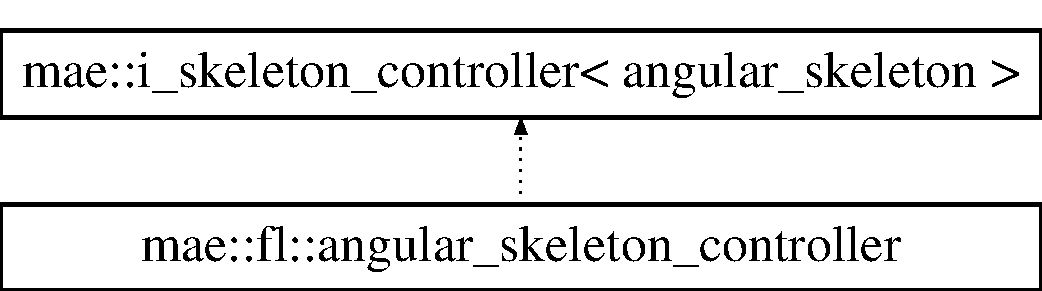
\includegraphics[height=2.000000cm]{classmae_1_1fl_1_1angular__skeleton__controller}
\end{center}
\end{figure}
\subsection*{Public Member Functions}
\begin{DoxyCompactItemize}
\item 
\hypertarget{classmae_1_1fl_1_1angular__skeleton__controller_a83357968cdb490b9032a32e9fef2765a}{{\bfseries angular\-\_\-skeleton\-\_\-controller} (bool debug=false)}\label{classmae_1_1fl_1_1angular__skeleton__controller_a83357968cdb490b9032a32e9fef2765a}

\item 
virtual std\-::shared\-\_\-ptr\\*
$<$ \hyperlink{classmae_1_1fl_1_1angular__skeleton}{angular\-\_\-skeleton} $>$ \hyperlink{classmae_1_1fl_1_1angular__skeleton__controller_afae922566ff1d48db88538bd4b0c0d19}{specified\-\_\-skeleton} (std\-::shared\-\_\-ptr$<$ \hyperlink{classmae_1_1general__skeleton}{general\-\_\-skeleton} $>$ skeleton)
\item 
virtual std\-::shared\-\_\-ptr\\*
$<$ \hyperlink{classmae_1_1fl_1_1angular__skeleton}{angular\-\_\-skeleton} $>$ \hyperlink{classmae_1_1fl_1_1angular__skeleton__controller_a51516cf6b196485b86505bc4ff70959e}{calculate\-\_\-angular\-\_\-skeleton} (std\-::shared\-\_\-ptr$<$ \hyperlink{classmae_1_1general__skeleton}{general\-\_\-skeleton} $>$ skeleton, std\-::shared\-\_\-ptr$<$ \hyperlink{classmae_1_1math_1_1vec3d}{mae\-::math\-::vec3d} $>$ u, std\-::shared\-\_\-ptr$<$ \hyperlink{classmae_1_1math_1_1vec3d}{mae\-::math\-::vec3d} $>$ r, std\-::shared\-\_\-ptr$<$ \hyperlink{classmae_1_1math_1_1vec3d}{mae\-::math\-::vec3d} $>$ t)
\end{DoxyCompactItemize}
\subsection*{Static Public Member Functions}
\begin{DoxyCompactItemize}
\item 
static std\-::shared\-\_\-ptr\\*
$<$ \hyperlink{classmae_1_1fl_1_1angular__joint}{angular\-\_\-joint} $>$ \hyperlink{classmae_1_1fl_1_1angular__skeleton__controller_a1cdea412c3d1a6cc585b2120f85abab4}{first\-\_\-degree\-\_\-md} (std\-::shared\-\_\-ptr$<$ \hyperlink{classmae_1_1general__skeleton}{general\-\_\-skeleton} $>$ skeleton, int adjacent\-\_\-joint, int outer\-\_\-joint, std\-::shared\-\_\-ptr$<$ \hyperlink{classmae_1_1math_1_1vec3d}{mae\-::math\-::vec3d} $>$ u, std\-::shared\-\_\-ptr$<$ \hyperlink{classmae_1_1math_1_1vec3d}{mae\-::math\-::vec3d} $>$ r, std\-::shared\-\_\-ptr$<$ \hyperlink{classmae_1_1math_1_1vec3d}{mae\-::math\-::vec3d} $>$ t, std\-::shared\-\_\-ptr$<$ \hyperlink{classmae_1_1math_1_1vec3d}{mae\-::math\-::vec3d} $>$ md)
\item 
static std\-::shared\-\_\-ptr\\*
$<$ \hyperlink{classmae_1_1fl_1_1angular__joint}{angular\-\_\-joint} $>$ \hyperlink{classmae_1_1fl_1_1angular__skeleton__controller_a3066e2bb6094c483f772c09facf05259}{first\-\_\-degree\-\_\-r} (std\-::shared\-\_\-ptr$<$ \hyperlink{classmae_1_1general__skeleton}{general\-\_\-skeleton} $>$ skeleton, int adjacent\-\_\-joint, int outer\-\_\-joint, std\-::shared\-\_\-ptr$<$ \hyperlink{classmae_1_1math_1_1vec3d}{mae\-::math\-::vec3d} $>$ u, std\-::shared\-\_\-ptr$<$ \hyperlink{classmae_1_1math_1_1vec3d}{mae\-::math\-::vec3d} $>$ r, std\-::shared\-\_\-ptr$<$ \hyperlink{classmae_1_1math_1_1vec3d}{mae\-::math\-::vec3d} $>$ t)
\item 
static std\-::shared\-\_\-ptr\\*
$<$ \hyperlink{classmae_1_1fl_1_1angular__joint}{angular\-\_\-joint} $>$ \hyperlink{classmae_1_1fl_1_1angular__skeleton__controller_ad1ab68acaaf4101ca13c2b50c639ed0a}{first\-\_\-degree} (std\-::shared\-\_\-ptr$<$ \hyperlink{classmae_1_1general__skeleton}{general\-\_\-skeleton} $>$ skeleton, int adjacent\-\_\-joint, int outer\-\_\-joint, std\-::shared\-\_\-ptr$<$ \hyperlink{classmae_1_1math_1_1vec3d}{mae\-::math\-::vec3d} $>$ u, std\-::shared\-\_\-ptr$<$ \hyperlink{classmae_1_1math_1_1vec3d}{mae\-::math\-::vec3d} $>$ r, std\-::shared\-\_\-ptr$<$ \hyperlink{classmae_1_1math_1_1vec3d}{mae\-::math\-::vec3d} $>$ t)
\item 
static std\-::shared\-\_\-ptr\\*
$<$ \hyperlink{classmae_1_1fl_1_1angular__joint}{angular\-\_\-joint} $>$ \hyperlink{classmae_1_1fl_1_1angular__skeleton__controller_a0a3eb90a79bb5eda18c6dba7a13972f8}{second\-\_\-degree} (std\-::shared\-\_\-ptr$<$ \hyperlink{classmae_1_1general__skeleton}{general\-\_\-skeleton} $>$ skeleton, int adjacent\-\_\-joint, int outer\-\_\-joint, int extremity\-\_\-joint, std\-::shared\-\_\-ptr$<$ \hyperlink{classmae_1_1math_1_1vec3d}{mae\-::math\-::vec3d} $>$ u, std\-::shared\-\_\-ptr$<$ \hyperlink{classmae_1_1math_1_1vec3d}{mae\-::math\-::vec3d} $>$ r, std\-::shared\-\_\-ptr$<$ \hyperlink{classmae_1_1math_1_1vec3d}{mae\-::math\-::vec3d} $>$ t)
\end{DoxyCompactItemize}


\subsection{Member Function Documentation}
\hypertarget{classmae_1_1fl_1_1angular__skeleton__controller_a51516cf6b196485b86505bc4ff70959e}{\index{mae\-::fl\-::angular\-\_\-skeleton\-\_\-controller@{mae\-::fl\-::angular\-\_\-skeleton\-\_\-controller}!calculate\-\_\-angular\-\_\-skeleton@{calculate\-\_\-angular\-\_\-skeleton}}
\index{calculate\-\_\-angular\-\_\-skeleton@{calculate\-\_\-angular\-\_\-skeleton}!mae::fl::angular_skeleton_controller@{mae\-::fl\-::angular\-\_\-skeleton\-\_\-controller}}
\subsubsection[{calculate\-\_\-angular\-\_\-skeleton}]{\setlength{\rightskip}{0pt plus 5cm}std\-::shared\-\_\-ptr$<$ {\bf angular\-\_\-skeleton} $>$ mae\-::fl\-::angular\-\_\-skeleton\-\_\-controller\-::calculate\-\_\-angular\-\_\-skeleton (
\begin{DoxyParamCaption}
\item[{std\-::shared\-\_\-ptr$<$ {\bf general\-\_\-skeleton} $>$}]{skeleton, }
\item[{std\-::shared\-\_\-ptr$<$ {\bf mae\-::math\-::vec3d} $>$}]{u, }
\item[{std\-::shared\-\_\-ptr$<$ {\bf mae\-::math\-::vec3d} $>$}]{r, }
\item[{std\-::shared\-\_\-ptr$<$ {\bf mae\-::math\-::vec3d} $>$}]{t}
\end{DoxyParamCaption}
)\hspace{0.3cm}{\ttfamily [virtual]}}}\label{classmae_1_1fl_1_1angular__skeleton__controller_a51516cf6b196485b86505bc4ff70959e}
Generates the angular skeleton from the general one.


\begin{DoxyParams}{Parameters}
{\em skeleton} & The general skeleton. \\
\hline
{\em u} & The u direction of the basis. \\
\hline
{\em r} & The r direction of the basis. \\
\hline
{\em t} & The t direction of the basis. \\
\hline
\end{DoxyParams}
\begin{DoxyReturn}{Returns}
The specified skeleton. 
\end{DoxyReturn}
\hypertarget{classmae_1_1fl_1_1angular__skeleton__controller_ad1ab68acaaf4101ca13c2b50c639ed0a}{\index{mae\-::fl\-::angular\-\_\-skeleton\-\_\-controller@{mae\-::fl\-::angular\-\_\-skeleton\-\_\-controller}!first\-\_\-degree@{first\-\_\-degree}}
\index{first\-\_\-degree@{first\-\_\-degree}!mae::fl::angular_skeleton_controller@{mae\-::fl\-::angular\-\_\-skeleton\-\_\-controller}}
\subsubsection[{first\-\_\-degree}]{\setlength{\rightskip}{0pt plus 5cm}std\-::shared\-\_\-ptr$<$ {\bf angular\-\_\-joint} $>$ mae\-::fl\-::angular\-\_\-skeleton\-\_\-controller\-::first\-\_\-degree (
\begin{DoxyParamCaption}
\item[{std\-::shared\-\_\-ptr$<$ {\bf general\-\_\-skeleton} $>$}]{skeleton, }
\item[{int}]{adjacent\-\_\-joint, }
\item[{int}]{outer\-\_\-joint, }
\item[{std\-::shared\-\_\-ptr$<$ {\bf mae\-::math\-::vec3d} $>$}]{u, }
\item[{std\-::shared\-\_\-ptr$<$ {\bf mae\-::math\-::vec3d} $>$}]{r, }
\item[{std\-::shared\-\_\-ptr$<$ {\bf mae\-::math\-::vec3d} $>$}]{t}
\end{DoxyParamCaption}
)\hspace{0.3cm}{\ttfamily [static]}}}\label{classmae_1_1fl_1_1angular__skeleton__controller_ad1ab68acaaf4101ca13c2b50c639ed0a}
Calculates the first degree joint which the general method.


\begin{DoxyParams}{Parameters}
{\em skeleton} & \\
\hline
{\em adjacent\-\_\-joint} & \\
\hline
{\em outer\-\_\-joint} & \\
\hline
{\em u} & \\
\hline
{\em r} & \\
\hline
{\em t} & \\
\hline
\end{DoxyParams}
\begin{DoxyReturn}{Returns}

\end{DoxyReturn}
\hypertarget{classmae_1_1fl_1_1angular__skeleton__controller_a1cdea412c3d1a6cc585b2120f85abab4}{\index{mae\-::fl\-::angular\-\_\-skeleton\-\_\-controller@{mae\-::fl\-::angular\-\_\-skeleton\-\_\-controller}!first\-\_\-degree\-\_\-md@{first\-\_\-degree\-\_\-md}}
\index{first\-\_\-degree\-\_\-md@{first\-\_\-degree\-\_\-md}!mae::fl::angular_skeleton_controller@{mae\-::fl\-::angular\-\_\-skeleton\-\_\-controller}}
\subsubsection[{first\-\_\-degree\-\_\-md}]{\setlength{\rightskip}{0pt plus 5cm}std\-::shared\-\_\-ptr$<$ {\bf angular\-\_\-joint} $>$ mae\-::fl\-::angular\-\_\-skeleton\-\_\-controller\-::first\-\_\-degree\-\_\-md (
\begin{DoxyParamCaption}
\item[{std\-::shared\-\_\-ptr$<$ {\bf general\-\_\-skeleton} $>$}]{skeleton, }
\item[{int}]{adjacent\-\_\-joint, }
\item[{int}]{outer\-\_\-joint, }
\item[{std\-::shared\-\_\-ptr$<$ {\bf mae\-::math\-::vec3d} $>$}]{u, }
\item[{std\-::shared\-\_\-ptr$<$ {\bf mae\-::math\-::vec3d} $>$}]{r, }
\item[{std\-::shared\-\_\-ptr$<$ {\bf mae\-::math\-::vec3d} $>$}]{t, }
\item[{std\-::shared\-\_\-ptr$<$ {\bf mae\-::math\-::vec3d} $>$}]{md}
\end{DoxyParamCaption}
)\hspace{0.3cm}{\ttfamily [static]}}}\label{classmae_1_1fl_1_1angular__skeleton__controller_a1cdea412c3d1a6cc585b2120f85abab4}
Calculates first degree joints using a main direction.


\begin{DoxyParams}{Parameters}
{\em skeleton} & \\
\hline
{\em adjacent\-\_\-joint} & \\
\hline
{\em outer\-\_\-joint} & \\
\hline
{\em u} & \\
\hline
{\em r} & \\
\hline
{\em t} & \\
\hline
{\em md} & \\
\hline
\end{DoxyParams}
\begin{DoxyReturn}{Returns}

\end{DoxyReturn}
\hypertarget{classmae_1_1fl_1_1angular__skeleton__controller_a3066e2bb6094c483f772c09facf05259}{\index{mae\-::fl\-::angular\-\_\-skeleton\-\_\-controller@{mae\-::fl\-::angular\-\_\-skeleton\-\_\-controller}!first\-\_\-degree\-\_\-r@{first\-\_\-degree\-\_\-r}}
\index{first\-\_\-degree\-\_\-r@{first\-\_\-degree\-\_\-r}!mae::fl::angular_skeleton_controller@{mae\-::fl\-::angular\-\_\-skeleton\-\_\-controller}}
\subsubsection[{first\-\_\-degree\-\_\-r}]{\setlength{\rightskip}{0pt plus 5cm}std\-::shared\-\_\-ptr$<$ {\bf angular\-\_\-joint} $>$ mae\-::fl\-::angular\-\_\-skeleton\-\_\-controller\-::first\-\_\-degree\-\_\-r (
\begin{DoxyParamCaption}
\item[{std\-::shared\-\_\-ptr$<$ {\bf general\-\_\-skeleton} $>$}]{skeleton, }
\item[{int}]{adjacent\-\_\-joint, }
\item[{int}]{outer\-\_\-joint, }
\item[{std\-::shared\-\_\-ptr$<$ {\bf mae\-::math\-::vec3d} $>$}]{u, }
\item[{std\-::shared\-\_\-ptr$<$ {\bf mae\-::math\-::vec3d} $>$}]{r, }
\item[{std\-::shared\-\_\-ptr$<$ {\bf mae\-::math\-::vec3d} $>$}]{t}
\end{DoxyParamCaption}
)\hspace{0.3cm}{\ttfamily [static]}}}\label{classmae_1_1fl_1_1angular__skeleton__controller_a3066e2bb6094c483f772c09facf05259}
Calculates the first degree joint using the plane to which r is the normal.


\begin{DoxyParams}{Parameters}
{\em skeleton} & \\
\hline
{\em adjacent\-\_\-joint} & \\
\hline
{\em outer\-\_\-joint} & \\
\hline
{\em u} & \\
\hline
{\em r} & \\
\hline
{\em t} & \\
\hline
\end{DoxyParams}
\begin{DoxyReturn}{Returns}

\end{DoxyReturn}
\hypertarget{classmae_1_1fl_1_1angular__skeleton__controller_a0a3eb90a79bb5eda18c6dba7a13972f8}{\index{mae\-::fl\-::angular\-\_\-skeleton\-\_\-controller@{mae\-::fl\-::angular\-\_\-skeleton\-\_\-controller}!second\-\_\-degree@{second\-\_\-degree}}
\index{second\-\_\-degree@{second\-\_\-degree}!mae::fl::angular_skeleton_controller@{mae\-::fl\-::angular\-\_\-skeleton\-\_\-controller}}
\subsubsection[{second\-\_\-degree}]{\setlength{\rightskip}{0pt plus 5cm}std\-::shared\-\_\-ptr$<$ {\bf angular\-\_\-joint} $>$ mae\-::fl\-::angular\-\_\-skeleton\-\_\-controller\-::second\-\_\-degree (
\begin{DoxyParamCaption}
\item[{std\-::shared\-\_\-ptr$<$ {\bf general\-\_\-skeleton} $>$}]{skeleton, }
\item[{int}]{adjacent\-\_\-joint, }
\item[{int}]{outer\-\_\-joint, }
\item[{int}]{extremity\-\_\-joint, }
\item[{std\-::shared\-\_\-ptr$<$ {\bf mae\-::math\-::vec3d} $>$}]{u, }
\item[{std\-::shared\-\_\-ptr$<$ {\bf mae\-::math\-::vec3d} $>$}]{r, }
\item[{std\-::shared\-\_\-ptr$<$ {\bf mae\-::math\-::vec3d} $>$}]{t}
\end{DoxyParamCaption}
)\hspace{0.3cm}{\ttfamily [static]}}}\label{classmae_1_1fl_1_1angular__skeleton__controller_a0a3eb90a79bb5eda18c6dba7a13972f8}
Calculates the second degree joint.


\begin{DoxyParams}{Parameters}
{\em skeleton} & \\
\hline
{\em adjacent\-\_\-joint} & \\
\hline
{\em outer\-\_\-joint} & \\
\hline
{\em extremity\-\_\-joint} & \\
\hline
{\em u} & \\
\hline
{\em r} & \\
\hline
{\em t} & \\
\hline
\end{DoxyParams}
\begin{DoxyReturn}{Returns}

\end{DoxyReturn}
\hypertarget{classmae_1_1fl_1_1angular__skeleton__controller_afae922566ff1d48db88538bd4b0c0d19}{\index{mae\-::fl\-::angular\-\_\-skeleton\-\_\-controller@{mae\-::fl\-::angular\-\_\-skeleton\-\_\-controller}!specified\-\_\-skeleton@{specified\-\_\-skeleton}}
\index{specified\-\_\-skeleton@{specified\-\_\-skeleton}!mae::fl::angular_skeleton_controller@{mae\-::fl\-::angular\-\_\-skeleton\-\_\-controller}}
\subsubsection[{specified\-\_\-skeleton}]{\setlength{\rightskip}{0pt plus 5cm}std\-::shared\-\_\-ptr$<$ {\bf angular\-\_\-skeleton} $>$ mae\-::fl\-::angular\-\_\-skeleton\-\_\-controller\-::specified\-\_\-skeleton (
\begin{DoxyParamCaption}
\item[{std\-::shared\-\_\-ptr$<$ {\bf general\-\_\-skeleton} $>$}]{skeleton}
\end{DoxyParamCaption}
)\hspace{0.3cm}{\ttfamily [virtual]}}}\label{classmae_1_1fl_1_1angular__skeleton__controller_afae922566ff1d48db88538bd4b0c0d19}
Generates the specified skeleton from the general skeleton.


\begin{DoxyParams}{Parameters}
{\em skeleton} & The general skeleton. \\
\hline
\end{DoxyParams}
\begin{DoxyReturn}{Returns}
The specified skeleton. 
\end{DoxyReturn}


Implements \hyperlink{classmae_1_1i__skeleton__controller_a5142885efc960951334765e2c66052c2}{mae\-::i\-\_\-skeleton\-\_\-controller$<$ angular\-\_\-skeleton $>$}.



The documentation for this class was generated from the following files\-:\begin{DoxyCompactItemize}
\item 
src/mae/fl/angular\-\_\-skeleton\-\_\-controller.\-hpp\item 
src/mae/fl/angular\-\_\-skeleton\-\_\-controller.\-cpp\end{DoxyCompactItemize}

\hypertarget{classmae_1_1fl_1_1laban_1_1ps_1_1area__part}{\section{mae\-:\-:fl\-:\-:laban\-:\-:ps\-:\-:area\-\_\-part Class Reference}
\label{classmae_1_1fl_1_1laban_1_1ps_1_1area__part}\index{mae\-::fl\-::laban\-::ps\-::area\-\_\-part@{mae\-::fl\-::laban\-::ps\-::area\-\_\-part}}
}
Inheritance diagram for mae\-:\-:fl\-:\-:laban\-:\-:ps\-:\-:area\-\_\-part\-:\begin{figure}[H]
\begin{center}
\leavevmode
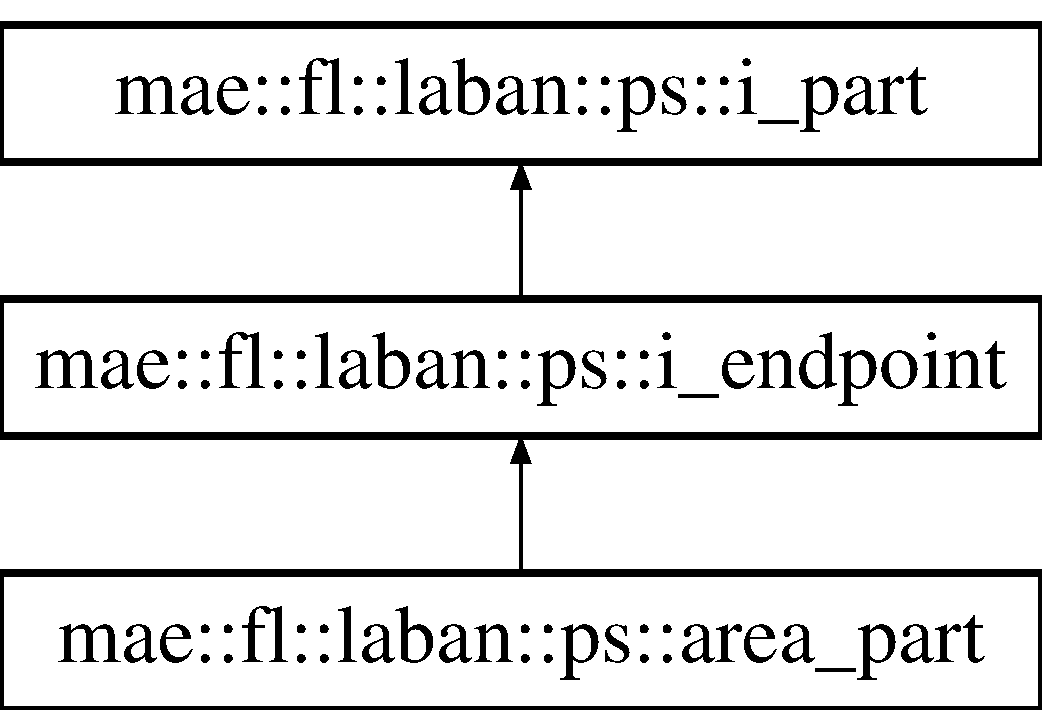
\includegraphics[height=3.000000cm]{classmae_1_1fl_1_1laban_1_1ps_1_1area__part}
\end{center}
\end{figure}
\subsection*{Public Member Functions}
\begin{DoxyCompactItemize}
\item 
\hyperlink{classmae_1_1fl_1_1laban_1_1ps_1_1area__part_a8bbf19849b499277fb4fce4547971ec0}{area\-\_\-part} (e\-\_\-area area)
\item 
e\-\_\-area \hyperlink{classmae_1_1fl_1_1laban_1_1ps_1_1area__part_a084e6beba901f615c5043b569389745d}{get\-\_\-area} () const 
\item 
virtual std\-::string \hyperlink{classmae_1_1fl_1_1laban_1_1ps_1_1area__part_a3ffd61d8cba76a5312a737a40dccb4ec}{xml} (unsigned int indent=0, std\-::string namesp=\char`\"{}\char`\"{}) const 
\item 
virtual std\-::string \hyperlink{classmae_1_1fl_1_1laban_1_1ps_1_1area__part_ad28ba26a5e96db2f23f07f974633fdf7}{svg} (std\-::string identifier, double posx, double posy, double width, double height, bool left=false) const 
\item 
virtual std\-::shared\-\_\-ptr\\*
$<$ \hyperlink{classmae_1_1fl_1_1laban_1_1ps_1_1i__endpoint}{i\-\_\-endpoint} $>$ \hyperlink{classmae_1_1fl_1_1laban_1_1ps_1_1area__part_ad3697cd7f8840ff9341da918cd7f84f5}{get\-\_\-fixed\-\_\-end} () const 
\item 
virtual bool \hyperlink{classmae_1_1fl_1_1laban_1_1ps_1_1area__part_aa223417cb9c21426014d0099f9fad72b}{equals} (std\-::shared\-\_\-ptr$<$ \hyperlink{classmae_1_1fl_1_1laban_1_1ps_1_1i__part}{i\-\_\-part} $>$ a) const 
\item 
virtual bool \hyperlink{classmae_1_1fl_1_1laban_1_1ps_1_1area__part_af1715756d2b703af8ea2d7549ff7a6fc}{equals} (std\-::shared\-\_\-ptr$<$ \hyperlink{classmae_1_1fl_1_1laban_1_1ps_1_1i__endpoint}{i\-\_\-endpoint} $>$ a) const 
\end{DoxyCompactItemize}


\subsection{Constructor \& Destructor Documentation}
\hypertarget{classmae_1_1fl_1_1laban_1_1ps_1_1area__part_a8bbf19849b499277fb4fce4547971ec0}{\index{mae\-::fl\-::laban\-::ps\-::area\-\_\-part@{mae\-::fl\-::laban\-::ps\-::area\-\_\-part}!area\-\_\-part@{area\-\_\-part}}
\index{area\-\_\-part@{area\-\_\-part}!mae::fl::laban::ps::area_part@{mae\-::fl\-::laban\-::ps\-::area\-\_\-part}}
\subsubsection[{area\-\_\-part}]{\setlength{\rightskip}{0pt plus 5cm}mae\-::fl\-::laban\-::ps\-::area\-\_\-part\-::area\-\_\-part (
\begin{DoxyParamCaption}
\item[{e\-\_\-area}]{area}
\end{DoxyParamCaption}
)}}\label{classmae_1_1fl_1_1laban_1_1ps_1_1area__part_a8bbf19849b499277fb4fce4547971ec0}
Creates a new area pre-\/sign.


\begin{DoxyParams}{Parameters}
{\em area} & The addressed area. \\
\hline
\end{DoxyParams}


\subsection{Member Function Documentation}
\hypertarget{classmae_1_1fl_1_1laban_1_1ps_1_1area__part_aa223417cb9c21426014d0099f9fad72b}{\index{mae\-::fl\-::laban\-::ps\-::area\-\_\-part@{mae\-::fl\-::laban\-::ps\-::area\-\_\-part}!equals@{equals}}
\index{equals@{equals}!mae::fl::laban::ps::area_part@{mae\-::fl\-::laban\-::ps\-::area\-\_\-part}}
\subsubsection[{equals}]{\setlength{\rightskip}{0pt plus 5cm}bool mae\-::fl\-::laban\-::ps\-::area\-\_\-part\-::equals (
\begin{DoxyParamCaption}
\item[{std\-::shared\-\_\-ptr$<$ {\bf i\-\_\-part} $>$}]{a}
\end{DoxyParamCaption}
) const\hspace{0.3cm}{\ttfamily [virtual]}}}\label{classmae_1_1fl_1_1laban_1_1ps_1_1area__part_aa223417cb9c21426014d0099f9fad72b}
Returns true if elements are equal.


\begin{DoxyParams}{Parameters}
{\em a} & The element to be compared to. \\
\hline
\end{DoxyParams}
\begin{DoxyReturn}{Returns}
True if equal. 
\end{DoxyReturn}


Implements \hyperlink{classmae_1_1fl_1_1laban_1_1ps_1_1i__endpoint_abc675b07d3ce69fbec362b2e792a1e06}{mae\-::fl\-::laban\-::ps\-::i\-\_\-endpoint}.

\hypertarget{classmae_1_1fl_1_1laban_1_1ps_1_1area__part_af1715756d2b703af8ea2d7549ff7a6fc}{\index{mae\-::fl\-::laban\-::ps\-::area\-\_\-part@{mae\-::fl\-::laban\-::ps\-::area\-\_\-part}!equals@{equals}}
\index{equals@{equals}!mae::fl::laban::ps::area_part@{mae\-::fl\-::laban\-::ps\-::area\-\_\-part}}
\subsubsection[{equals}]{\setlength{\rightskip}{0pt plus 5cm}bool mae\-::fl\-::laban\-::ps\-::area\-\_\-part\-::equals (
\begin{DoxyParamCaption}
\item[{std\-::shared\-\_\-ptr$<$ {\bf i\-\_\-endpoint} $>$}]{a}
\end{DoxyParamCaption}
) const\hspace{0.3cm}{\ttfamily [virtual]}}}\label{classmae_1_1fl_1_1laban_1_1ps_1_1area__part_af1715756d2b703af8ea2d7549ff7a6fc}
Returns true if elements are equal.


\begin{DoxyParams}{Parameters}
{\em a} & The element to be compared to. \\
\hline
\end{DoxyParams}
\begin{DoxyReturn}{Returns}
True if equal. 
\end{DoxyReturn}


Implements \hyperlink{classmae_1_1fl_1_1laban_1_1ps_1_1i__endpoint_aeffb14c43728d2ef094122f3d0278455}{mae\-::fl\-::laban\-::ps\-::i\-\_\-endpoint}.

\hypertarget{classmae_1_1fl_1_1laban_1_1ps_1_1area__part_a084e6beba901f615c5043b569389745d}{\index{mae\-::fl\-::laban\-::ps\-::area\-\_\-part@{mae\-::fl\-::laban\-::ps\-::area\-\_\-part}!get\-\_\-area@{get\-\_\-area}}
\index{get\-\_\-area@{get\-\_\-area}!mae::fl::laban::ps::area_part@{mae\-::fl\-::laban\-::ps\-::area\-\_\-part}}
\subsubsection[{get\-\_\-area}]{\setlength{\rightskip}{0pt plus 5cm}e\-\_\-area mae\-::fl\-::laban\-::ps\-::area\-\_\-part\-::get\-\_\-area (
\begin{DoxyParamCaption}
{}
\end{DoxyParamCaption}
) const}}\label{classmae_1_1fl_1_1laban_1_1ps_1_1area__part_a084e6beba901f615c5043b569389745d}
Returns the addressed area.

\begin{DoxyReturn}{Returns}

\end{DoxyReturn}
\hypertarget{classmae_1_1fl_1_1laban_1_1ps_1_1area__part_ad3697cd7f8840ff9341da918cd7f84f5}{\index{mae\-::fl\-::laban\-::ps\-::area\-\_\-part@{mae\-::fl\-::laban\-::ps\-::area\-\_\-part}!get\-\_\-fixed\-\_\-end@{get\-\_\-fixed\-\_\-end}}
\index{get\-\_\-fixed\-\_\-end@{get\-\_\-fixed\-\_\-end}!mae::fl::laban::ps::area_part@{mae\-::fl\-::laban\-::ps\-::area\-\_\-part}}
\subsubsection[{get\-\_\-fixed\-\_\-end}]{\setlength{\rightskip}{0pt plus 5cm}std\-::shared\-\_\-ptr$<$ {\bf i\-\_\-endpoint} $>$ mae\-::fl\-::laban\-::ps\-::area\-\_\-part\-::get\-\_\-fixed\-\_\-end (
\begin{DoxyParamCaption}
{}
\end{DoxyParamCaption}
) const\hspace{0.3cm}{\ttfamily [virtual]}}}\label{classmae_1_1fl_1_1laban_1_1ps_1_1area__part_ad3697cd7f8840ff9341da918cd7f84f5}
Returns the successor of the current endpoint (which is the default extremity endpoint). If the endpoint is the end of the extremity null is returned.

\begin{DoxyReturn}{Returns}
The successor element. 
\end{DoxyReturn}


Implements \hyperlink{classmae_1_1fl_1_1laban_1_1ps_1_1i__endpoint_a0938824cc5892b072636c3b52352b3f2}{mae\-::fl\-::laban\-::ps\-::i\-\_\-endpoint}.

\hypertarget{classmae_1_1fl_1_1laban_1_1ps_1_1area__part_ad28ba26a5e96db2f23f07f974633fdf7}{\index{mae\-::fl\-::laban\-::ps\-::area\-\_\-part@{mae\-::fl\-::laban\-::ps\-::area\-\_\-part}!svg@{svg}}
\index{svg@{svg}!mae::fl::laban::ps::area_part@{mae\-::fl\-::laban\-::ps\-::area\-\_\-part}}
\subsubsection[{svg}]{\setlength{\rightskip}{0pt plus 5cm}std\-::string mae\-::fl\-::laban\-::ps\-::area\-\_\-part\-::svg (
\begin{DoxyParamCaption}
\item[{std\-::string}]{identifier, }
\item[{double}]{posx, }
\item[{double}]{posy, }
\item[{double}]{width, }
\item[{double}]{height, }
\item[{bool}]{left = {\ttfamily false}}
\end{DoxyParamCaption}
) const\hspace{0.3cm}{\ttfamily [virtual]}}}\label{classmae_1_1fl_1_1laban_1_1ps_1_1area__part_ad28ba26a5e96db2f23f07f974633fdf7}
Returns the S\-V\-G representation for this symbol.


\begin{DoxyParams}{Parameters}
{\em posx} & The x position. \\
\hline
{\em posy} & The y position. \\
\hline
{\em width} & The width. \\
\hline
{\em height} & The height. \\
\hline
\end{DoxyParams}
\begin{DoxyReturn}{Returns}
The S\-V\-G. 
\end{DoxyReturn}


Implements \hyperlink{classmae_1_1fl_1_1laban_1_1ps_1_1i__part_a78227d5ecd87655a7a9454c68f470368}{mae\-::fl\-::laban\-::ps\-::i\-\_\-part}.

\hypertarget{classmae_1_1fl_1_1laban_1_1ps_1_1area__part_a3ffd61d8cba76a5312a737a40dccb4ec}{\index{mae\-::fl\-::laban\-::ps\-::area\-\_\-part@{mae\-::fl\-::laban\-::ps\-::area\-\_\-part}!xml@{xml}}
\index{xml@{xml}!mae::fl::laban::ps::area_part@{mae\-::fl\-::laban\-::ps\-::area\-\_\-part}}
\subsubsection[{xml}]{\setlength{\rightskip}{0pt plus 5cm}std\-::string mae\-::fl\-::laban\-::ps\-::area\-\_\-part\-::xml (
\begin{DoxyParamCaption}
\item[{unsigned int}]{indent = {\ttfamily 0}, }
\item[{std\-::string}]{namesp = {\ttfamily \char`\"{}\char`\"{}}}
\end{DoxyParamCaption}
) const\hspace{0.3cm}{\ttfamily [virtual]}}}\label{classmae_1_1fl_1_1laban_1_1ps_1_1area__part_a3ffd61d8cba76a5312a737a40dccb4ec}
Returns the X\-M\-L representation for this element.


\begin{DoxyParams}{Parameters}
{\em indent} & The applied indent. \\
\hline
{\em namesp} & The prefixed X\-M\-L namespace.\\
\hline
\end{DoxyParams}
\begin{DoxyReturn}{Returns}
The X\-M\-L string. 
\end{DoxyReturn}


Implements \hyperlink{classmae_1_1fl_1_1laban_1_1ps_1_1i__endpoint_a1af7dbd05400cbdd7f9f45ef75dd38d6}{mae\-::fl\-::laban\-::ps\-::i\-\_\-endpoint}.



The documentation for this class was generated from the following files\-:\begin{DoxyCompactItemize}
\item 
src/mae/fl/laban/ps/area\-\_\-part.\-hpp\item 
src/mae/fl/laban/ps/area\-\_\-part.\-cpp\end{DoxyCompactItemize}

\hypertarget{classmae_1_1math_1_1basis}{\section{mae\-:\-:math\-:\-:basis Class Reference}
\label{classmae_1_1math_1_1basis}\index{mae\-::math\-::basis@{mae\-::math\-::basis}}
}
\subsection*{Public Member Functions}
\begin{DoxyCompactItemize}
\item 
\hyperlink{classmae_1_1math_1_1basis_a20b328000b2a05065b2b3fd3f01dc1db}{basis} ()
\item 
\hyperlink{classmae_1_1math_1_1basis_a03cc7a891aee20d97b35773f3e0201a5}{basis} (std\-::shared\-\_\-ptr$<$ \hyperlink{classmae_1_1math_1_1vec3d}{vec3d} $>$ position\-\_\-vector, std\-::shared\-\_\-ptr$<$ \hyperlink{classmae_1_1math_1_1vec3d}{vec3d} $>$ u, std\-::shared\-\_\-ptr$<$ \hyperlink{classmae_1_1math_1_1vec3d}{vec3d} $>$ r, std\-::shared\-\_\-ptr$<$ \hyperlink{classmae_1_1math_1_1vec3d}{vec3d} $>$ t)
\item 
virtual std\-::shared\-\_\-ptr$<$ \hyperlink{classmae_1_1math_1_1vec3d}{vec3d} $>$ \hyperlink{classmae_1_1math_1_1basis_a31db97f8289074bcc274dbf626f3f9b6}{get\-\_\-u} () const 
\item 
virtual std\-::shared\-\_\-ptr$<$ \hyperlink{classmae_1_1math_1_1vec3d}{vec3d} $>$ \hyperlink{classmae_1_1math_1_1basis_adeaf5ae18e066bd20ddcc4be8a844d80}{get\-\_\-r} () const 
\item 
virtual std\-::shared\-\_\-ptr$<$ \hyperlink{classmae_1_1math_1_1vec3d}{vec3d} $>$ \hyperlink{classmae_1_1math_1_1basis_a3c9af401b04f96c4d765a43c207c3916}{get\-\_\-t} () const 
\item 
virtual std\-::shared\-\_\-ptr$<$ \hyperlink{classmae_1_1math_1_1vec3d}{vec3d} $>$ \hyperlink{classmae_1_1math_1_1basis_a1343e0d24ce24d73d41d8ec316837b5f}{get\-\_\-position\-\_\-vector} () const 
\item 
virtual void \hyperlink{classmae_1_1math_1_1basis_a09ea870f8765b92d200c74893f554253}{set\-\_\-u} (std\-::shared\-\_\-ptr$<$ \hyperlink{classmae_1_1math_1_1vec3d}{vec3d} $>$ u)
\item 
virtual void \hyperlink{classmae_1_1math_1_1basis_a08992f887e7f7691f53fe31f4245deb9}{set\-\_\-r} (std\-::shared\-\_\-ptr$<$ \hyperlink{classmae_1_1math_1_1vec3d}{vec3d} $>$ r)
\item 
virtual void \hyperlink{classmae_1_1math_1_1basis_a0574f45a44b8fc1c38bf1ef603e621a9}{set\-\_\-t} (std\-::shared\-\_\-ptr$<$ \hyperlink{classmae_1_1math_1_1vec3d}{vec3d} $>$ t)
\item 
virtual void \hyperlink{classmae_1_1math_1_1basis_a89b97015efedce5e4c0b178ebae19e2f}{set\-\_\-position\-\_\-vector} (std\-::shared\-\_\-ptr$<$ \hyperlink{classmae_1_1math_1_1vec3d}{vec3d} $>$ position\-\_\-vector)
\item 
virtual std\-::string \hyperlink{classmae_1_1math_1_1basis_a070c4a1ad93988e38b1b47ef31bb6c7d}{str} () const 
\end{DoxyCompactItemize}
\subsection*{Friends}
\begin{DoxyCompactItemize}
\item 
std\-::ostream \& \hyperlink{classmae_1_1math_1_1basis_a0daa15acafe29d2f46fdeba231948ff5}{operator$<$$<$} (std\-::ostream \&os, const std\-::shared\-\_\-ptr$<$ \hyperlink{classmae_1_1math_1_1basis}{basis} $>$ \&obj)
\item 
std\-::ostream \& \hyperlink{classmae_1_1math_1_1basis_a53ed94899ec5639af128068432d09fde}{operator$<$$<$} (std\-::ostream \&os, const \hyperlink{classmae_1_1math_1_1basis}{basis} \&obj)
\end{DoxyCompactItemize}


\subsection{Constructor \& Destructor Documentation}
\hypertarget{classmae_1_1math_1_1basis_a20b328000b2a05065b2b3fd3f01dc1db}{\index{mae\-::math\-::basis@{mae\-::math\-::basis}!basis@{basis}}
\index{basis@{basis}!mae::math::basis@{mae\-::math\-::basis}}
\subsubsection[{basis}]{\setlength{\rightskip}{0pt plus 5cm}mae\-::math\-::basis\-::basis (
\begin{DoxyParamCaption}
{}
\end{DoxyParamCaption}
)}}\label{classmae_1_1math_1_1basis_a20b328000b2a05065b2b3fd3f01dc1db}
Creates a new basis with no vectors set. \hypertarget{classmae_1_1math_1_1basis_a03cc7a891aee20d97b35773f3e0201a5}{\index{mae\-::math\-::basis@{mae\-::math\-::basis}!basis@{basis}}
\index{basis@{basis}!mae::math::basis@{mae\-::math\-::basis}}
\subsubsection[{basis}]{\setlength{\rightskip}{0pt plus 5cm}mae\-::math\-::basis\-::basis (
\begin{DoxyParamCaption}
\item[{std\-::shared\-\_\-ptr$<$ {\bf vec3d} $>$}]{position\-\_\-vector, }
\item[{std\-::shared\-\_\-ptr$<$ {\bf vec3d} $>$}]{u, }
\item[{std\-::shared\-\_\-ptr$<$ {\bf vec3d} $>$}]{r, }
\item[{std\-::shared\-\_\-ptr$<$ {\bf vec3d} $>$}]{t}
\end{DoxyParamCaption}
)}}\label{classmae_1_1math_1_1basis_a03cc7a891aee20d97b35773f3e0201a5}
Creates a new coordinate basis.


\begin{DoxyParams}{Parameters}
{\em position\-\_\-vector} & The position vector of the basis. \\
\hline
{\em u} & The first direction. \\
\hline
{\em r} & The second direction. \\
\hline
{\em t} & The third direction. \\
\hline
\end{DoxyParams}


\subsection{Member Function Documentation}
\hypertarget{classmae_1_1math_1_1basis_a1343e0d24ce24d73d41d8ec316837b5f}{\index{mae\-::math\-::basis@{mae\-::math\-::basis}!get\-\_\-position\-\_\-vector@{get\-\_\-position\-\_\-vector}}
\index{get\-\_\-position\-\_\-vector@{get\-\_\-position\-\_\-vector}!mae::math::basis@{mae\-::math\-::basis}}
\subsubsection[{get\-\_\-position\-\_\-vector}]{\setlength{\rightskip}{0pt plus 5cm}std\-::shared\-\_\-ptr$<$ {\bf vec3d} $>$ mae\-::math\-::basis\-::get\-\_\-position\-\_\-vector (
\begin{DoxyParamCaption}
{}
\end{DoxyParamCaption}
) const\hspace{0.3cm}{\ttfamily [virtual]}}}\label{classmae_1_1math_1_1basis_a1343e0d24ce24d73d41d8ec316837b5f}
Returns the position vector of the basis.

\begin{DoxyReturn}{Returns}
The position\-\_\-vector. 
\end{DoxyReturn}
\hypertarget{classmae_1_1math_1_1basis_adeaf5ae18e066bd20ddcc4be8a844d80}{\index{mae\-::math\-::basis@{mae\-::math\-::basis}!get\-\_\-r@{get\-\_\-r}}
\index{get\-\_\-r@{get\-\_\-r}!mae::math::basis@{mae\-::math\-::basis}}
\subsubsection[{get\-\_\-r}]{\setlength{\rightskip}{0pt plus 5cm}std\-::shared\-\_\-ptr$<$ {\bf vec3d} $>$ mae\-::math\-::basis\-::get\-\_\-r (
\begin{DoxyParamCaption}
{}
\end{DoxyParamCaption}
) const\hspace{0.3cm}{\ttfamily [virtual]}}}\label{classmae_1_1math_1_1basis_adeaf5ae18e066bd20ddcc4be8a844d80}
Returns the second component of the basis.

\begin{DoxyReturn}{Returns}
The r. 
\end{DoxyReturn}
\hypertarget{classmae_1_1math_1_1basis_a3c9af401b04f96c4d765a43c207c3916}{\index{mae\-::math\-::basis@{mae\-::math\-::basis}!get\-\_\-t@{get\-\_\-t}}
\index{get\-\_\-t@{get\-\_\-t}!mae::math::basis@{mae\-::math\-::basis}}
\subsubsection[{get\-\_\-t}]{\setlength{\rightskip}{0pt plus 5cm}std\-::shared\-\_\-ptr$<$ {\bf vec3d} $>$ mae\-::math\-::basis\-::get\-\_\-t (
\begin{DoxyParamCaption}
{}
\end{DoxyParamCaption}
) const\hspace{0.3cm}{\ttfamily [virtual]}}}\label{classmae_1_1math_1_1basis_a3c9af401b04f96c4d765a43c207c3916}
Returns the third component of the basis.

\begin{DoxyReturn}{Returns}
The t. 
\end{DoxyReturn}
\hypertarget{classmae_1_1math_1_1basis_a31db97f8289074bcc274dbf626f3f9b6}{\index{mae\-::math\-::basis@{mae\-::math\-::basis}!get\-\_\-u@{get\-\_\-u}}
\index{get\-\_\-u@{get\-\_\-u}!mae::math::basis@{mae\-::math\-::basis}}
\subsubsection[{get\-\_\-u}]{\setlength{\rightskip}{0pt plus 5cm}std\-::shared\-\_\-ptr$<$ {\bf vec3d} $>$ mae\-::math\-::basis\-::get\-\_\-u (
\begin{DoxyParamCaption}
{}
\end{DoxyParamCaption}
) const\hspace{0.3cm}{\ttfamily [virtual]}}}\label{classmae_1_1math_1_1basis_a31db97f8289074bcc274dbf626f3f9b6}
Returns the first component of the basis.

\begin{DoxyReturn}{Returns}
The u. 
\end{DoxyReturn}
\hypertarget{classmae_1_1math_1_1basis_a89b97015efedce5e4c0b178ebae19e2f}{\index{mae\-::math\-::basis@{mae\-::math\-::basis}!set\-\_\-position\-\_\-vector@{set\-\_\-position\-\_\-vector}}
\index{set\-\_\-position\-\_\-vector@{set\-\_\-position\-\_\-vector}!mae::math::basis@{mae\-::math\-::basis}}
\subsubsection[{set\-\_\-position\-\_\-vector}]{\setlength{\rightskip}{0pt plus 5cm}void mae\-::math\-::basis\-::set\-\_\-position\-\_\-vector (
\begin{DoxyParamCaption}
\item[{std\-::shared\-\_\-ptr$<$ {\bf vec3d} $>$}]{position\-\_\-vector}
\end{DoxyParamCaption}
)\hspace{0.3cm}{\ttfamily [virtual]}}}\label{classmae_1_1math_1_1basis_a89b97015efedce5e4c0b178ebae19e2f}
Sets the position\-\_\-vector for the basis.


\begin{DoxyParams}{Parameters}
{\em position\-\_\-vector} & The t. \\
\hline
\end{DoxyParams}
\hypertarget{classmae_1_1math_1_1basis_a08992f887e7f7691f53fe31f4245deb9}{\index{mae\-::math\-::basis@{mae\-::math\-::basis}!set\-\_\-r@{set\-\_\-r}}
\index{set\-\_\-r@{set\-\_\-r}!mae::math::basis@{mae\-::math\-::basis}}
\subsubsection[{set\-\_\-r}]{\setlength{\rightskip}{0pt plus 5cm}void mae\-::math\-::basis\-::set\-\_\-r (
\begin{DoxyParamCaption}
\item[{std\-::shared\-\_\-ptr$<$ {\bf vec3d} $>$}]{r}
\end{DoxyParamCaption}
)\hspace{0.3cm}{\ttfamily [virtual]}}}\label{classmae_1_1math_1_1basis_a08992f887e7f7691f53fe31f4245deb9}
Sets the second component for the basis.


\begin{DoxyParams}{Parameters}
{\em r} & The r. \\
\hline
\end{DoxyParams}
\hypertarget{classmae_1_1math_1_1basis_a0574f45a44b8fc1c38bf1ef603e621a9}{\index{mae\-::math\-::basis@{mae\-::math\-::basis}!set\-\_\-t@{set\-\_\-t}}
\index{set\-\_\-t@{set\-\_\-t}!mae::math::basis@{mae\-::math\-::basis}}
\subsubsection[{set\-\_\-t}]{\setlength{\rightskip}{0pt plus 5cm}void mae\-::math\-::basis\-::set\-\_\-t (
\begin{DoxyParamCaption}
\item[{std\-::shared\-\_\-ptr$<$ {\bf vec3d} $>$}]{t}
\end{DoxyParamCaption}
)\hspace{0.3cm}{\ttfamily [virtual]}}}\label{classmae_1_1math_1_1basis_a0574f45a44b8fc1c38bf1ef603e621a9}
Sets the third component for the basis.


\begin{DoxyParams}{Parameters}
{\em t} & The t. \\
\hline
\end{DoxyParams}
\hypertarget{classmae_1_1math_1_1basis_a09ea870f8765b92d200c74893f554253}{\index{mae\-::math\-::basis@{mae\-::math\-::basis}!set\-\_\-u@{set\-\_\-u}}
\index{set\-\_\-u@{set\-\_\-u}!mae::math::basis@{mae\-::math\-::basis}}
\subsubsection[{set\-\_\-u}]{\setlength{\rightskip}{0pt plus 5cm}void mae\-::math\-::basis\-::set\-\_\-u (
\begin{DoxyParamCaption}
\item[{std\-::shared\-\_\-ptr$<$ {\bf vec3d} $>$}]{u}
\end{DoxyParamCaption}
)\hspace{0.3cm}{\ttfamily [virtual]}}}\label{classmae_1_1math_1_1basis_a09ea870f8765b92d200c74893f554253}
Sets the first component for the basis.


\begin{DoxyParams}{Parameters}
{\em u} & The u. \\
\hline
\end{DoxyParams}
\hypertarget{classmae_1_1math_1_1basis_a070c4a1ad93988e38b1b47ef31bb6c7d}{\index{mae\-::math\-::basis@{mae\-::math\-::basis}!str@{str}}
\index{str@{str}!mae::math::basis@{mae\-::math\-::basis}}
\subsubsection[{str}]{\setlength{\rightskip}{0pt plus 5cm}std\-::string mae\-::math\-::basis\-::str (
\begin{DoxyParamCaption}
{}
\end{DoxyParamCaption}
) const\hspace{0.3cm}{\ttfamily [virtual]}}}\label{classmae_1_1math_1_1basis_a070c4a1ad93988e38b1b47ef31bb6c7d}
Returns the string representation for this object.

\begin{DoxyReturn}{Returns}
The string. 
\end{DoxyReturn}


\subsection{Friends And Related Function Documentation}
\hypertarget{classmae_1_1math_1_1basis_a0daa15acafe29d2f46fdeba231948ff5}{\index{mae\-::math\-::basis@{mae\-::math\-::basis}!operator$<$$<$@{operator$<$$<$}}
\index{operator$<$$<$@{operator$<$$<$}!mae::math::basis@{mae\-::math\-::basis}}
\subsubsection[{operator$<$$<$}]{\setlength{\rightskip}{0pt plus 5cm}std\-::ostream\& operator$<$$<$ (
\begin{DoxyParamCaption}
\item[{std\-::ostream \&}]{os, }
\item[{const std\-::shared\-\_\-ptr$<$ {\bf basis} $>$ \&}]{obj}
\end{DoxyParamCaption}
)\hspace{0.3cm}{\ttfamily [friend]}}}\label{classmae_1_1math_1_1basis_a0daa15acafe29d2f46fdeba231948ff5}
Prints the object to the stream.


\begin{DoxyParams}{Parameters}
{\em os} & \\
\hline
{\em obj} & The object to be printed. \\
\hline
\end{DoxyParams}
\begin{DoxyReturn}{Returns}

\end{DoxyReturn}
\hypertarget{classmae_1_1math_1_1basis_a53ed94899ec5639af128068432d09fde}{\index{mae\-::math\-::basis@{mae\-::math\-::basis}!operator$<$$<$@{operator$<$$<$}}
\index{operator$<$$<$@{operator$<$$<$}!mae::math::basis@{mae\-::math\-::basis}}
\subsubsection[{operator$<$$<$}]{\setlength{\rightskip}{0pt plus 5cm}std\-::ostream\& operator$<$$<$ (
\begin{DoxyParamCaption}
\item[{std\-::ostream \&}]{os, }
\item[{const {\bf basis} \&}]{obj}
\end{DoxyParamCaption}
)\hspace{0.3cm}{\ttfamily [friend]}}}\label{classmae_1_1math_1_1basis_a53ed94899ec5639af128068432d09fde}
Prints the object to the stream.


\begin{DoxyParams}{Parameters}
{\em os} & \\
\hline
{\em obj} & The object to be printed. \\
\hline
\end{DoxyParams}
\begin{DoxyReturn}{Returns}

\end{DoxyReturn}


The documentation for this class was generated from the following files\-:\begin{DoxyCompactItemize}
\item 
src/mae/math/basis.\-hpp\item 
src/mae/math/basis.\-cpp\end{DoxyCompactItemize}

\hypertarget{classmae_1_1fl_1_1laban_1_1ps_1_1body__part}{\section{mae\-:\-:fl\-:\-:laban\-:\-:ps\-:\-:body\-\_\-part Class Reference}
\label{classmae_1_1fl_1_1laban_1_1ps_1_1body__part}\index{mae\-::fl\-::laban\-::ps\-::body\-\_\-part@{mae\-::fl\-::laban\-::ps\-::body\-\_\-part}}
}
Inheritance diagram for mae\-:\-:fl\-:\-:laban\-:\-:ps\-:\-:body\-\_\-part\-:\begin{figure}[H]
\begin{center}
\leavevmode
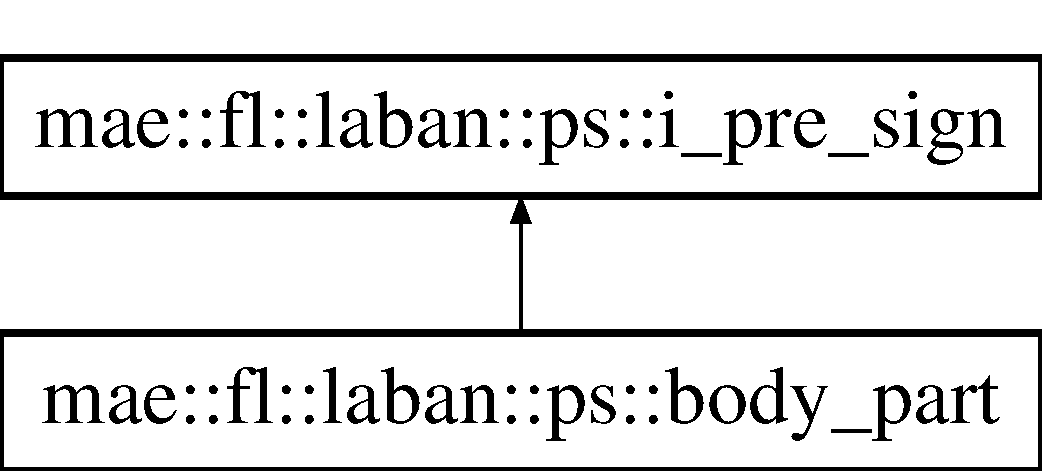
\includegraphics[height=2.000000cm]{classmae_1_1fl_1_1laban_1_1ps_1_1body__part}
\end{center}
\end{figure}
\subsection*{Public Member Functions}
\begin{DoxyCompactItemize}
\item 
\hyperlink{classmae_1_1fl_1_1laban_1_1ps_1_1body__part_a25f3ba48e88581c43d57de6d865c0aad}{body\-\_\-part} (e\-\_\-side side, std\-::shared\-\_\-ptr$<$ \hyperlink{classmae_1_1fl_1_1laban_1_1ps_1_1i__part}{i\-\_\-part} $>$ part)
\item 
e\-\_\-side \hyperlink{classmae_1_1fl_1_1laban_1_1ps_1_1body__part_afbfc05dba32b1790f6157bb8c3532b08}{get\-\_\-side} () const 
\item 
std\-::shared\-\_\-ptr$<$ \hyperlink{classmae_1_1fl_1_1laban_1_1ps_1_1i__part}{i\-\_\-part} $>$ \hyperlink{classmae_1_1fl_1_1laban_1_1ps_1_1body__part_a5a5daa5256abcf6372ff26710fcbb261}{get\-\_\-part} () const 
\item 
virtual std\-::string \hyperlink{classmae_1_1fl_1_1laban_1_1ps_1_1body__part_add0b077b3b062220ec16741b603e2747}{xml} (unsigned int indent=0, std\-::string namesp=\char`\"{}\char`\"{}) const 
\item 
virtual std\-::string \hyperlink{classmae_1_1fl_1_1laban_1_1ps_1_1body__part_aad8376f76f0cc424da8569ada4579c9a}{svg} (std\-::string identifier, double posx, double posy, double width, double height, bool left=false) const 
\item 
virtual bool \hyperlink{classmae_1_1fl_1_1laban_1_1ps_1_1body__part_abc74bc42375b203522754607f85851c4}{equals} (std\-::shared\-\_\-ptr$<$ \hyperlink{classmae_1_1fl_1_1laban_1_1ps_1_1i__pre__sign}{i\-\_\-pre\-\_\-sign} $>$ a) const 
\end{DoxyCompactItemize}


\subsection{Constructor \& Destructor Documentation}
\hypertarget{classmae_1_1fl_1_1laban_1_1ps_1_1body__part_a25f3ba48e88581c43d57de6d865c0aad}{\index{mae\-::fl\-::laban\-::ps\-::body\-\_\-part@{mae\-::fl\-::laban\-::ps\-::body\-\_\-part}!body\-\_\-part@{body\-\_\-part}}
\index{body\-\_\-part@{body\-\_\-part}!mae::fl::laban::ps::body_part@{mae\-::fl\-::laban\-::ps\-::body\-\_\-part}}
\subsubsection[{body\-\_\-part}]{\setlength{\rightskip}{0pt plus 5cm}mae\-::fl\-::laban\-::ps\-::body\-\_\-part\-::body\-\_\-part (
\begin{DoxyParamCaption}
\item[{e\-\_\-side}]{side, }
\item[{std\-::shared\-\_\-ptr$<$ {\bf i\-\_\-part} $>$}]{part}
\end{DoxyParamCaption}
)}}\label{classmae_1_1fl_1_1laban_1_1ps_1_1body__part_a25f3ba48e88581c43d57de6d865c0aad}
Creates a new body part pre-\/sign. It contains of a specific part and a side. If the side has no meaning to the part (e.\-g. head) is should be set to N\-O\-N\-E.


\begin{DoxyParams}{Parameters}
{\em side} & The side of the body. \\
\hline
{\em part} & The body part. \\
\hline
\end{DoxyParams}


\subsection{Member Function Documentation}
\hypertarget{classmae_1_1fl_1_1laban_1_1ps_1_1body__part_abc74bc42375b203522754607f85851c4}{\index{mae\-::fl\-::laban\-::ps\-::body\-\_\-part@{mae\-::fl\-::laban\-::ps\-::body\-\_\-part}!equals@{equals}}
\index{equals@{equals}!mae::fl::laban::ps::body_part@{mae\-::fl\-::laban\-::ps\-::body\-\_\-part}}
\subsubsection[{equals}]{\setlength{\rightskip}{0pt plus 5cm}bool mae\-::fl\-::laban\-::ps\-::body\-\_\-part\-::equals (
\begin{DoxyParamCaption}
\item[{std\-::shared\-\_\-ptr$<$ {\bf i\-\_\-pre\-\_\-sign} $>$}]{a}
\end{DoxyParamCaption}
) const\hspace{0.3cm}{\ttfamily [virtual]}}}\label{classmae_1_1fl_1_1laban_1_1ps_1_1body__part_abc74bc42375b203522754607f85851c4}
Returns true if elements are equal.


\begin{DoxyParams}{Parameters}
{\em a} & The element to be compared to. \\
\hline
\end{DoxyParams}
\begin{DoxyReturn}{Returns}
True if equal. 
\end{DoxyReturn}


Implements \hyperlink{classmae_1_1fl_1_1laban_1_1ps_1_1i__pre__sign_a8e3342fe33b6bd050d613330da30213d}{mae\-::fl\-::laban\-::ps\-::i\-\_\-pre\-\_\-sign}.

\hypertarget{classmae_1_1fl_1_1laban_1_1ps_1_1body__part_a5a5daa5256abcf6372ff26710fcbb261}{\index{mae\-::fl\-::laban\-::ps\-::body\-\_\-part@{mae\-::fl\-::laban\-::ps\-::body\-\_\-part}!get\-\_\-part@{get\-\_\-part}}
\index{get\-\_\-part@{get\-\_\-part}!mae::fl::laban::ps::body_part@{mae\-::fl\-::laban\-::ps\-::body\-\_\-part}}
\subsubsection[{get\-\_\-part}]{\setlength{\rightskip}{0pt plus 5cm}std\-::shared\-\_\-ptr$<$ {\bf i\-\_\-part} $>$ mae\-::fl\-::laban\-::ps\-::body\-\_\-part\-::get\-\_\-part (
\begin{DoxyParamCaption}
{}
\end{DoxyParamCaption}
) const}}\label{classmae_1_1fl_1_1laban_1_1ps_1_1body__part_a5a5daa5256abcf6372ff26710fcbb261}
Returns the addressed body part. \begin{DoxyReturn}{Returns}

\end{DoxyReturn}
\hypertarget{classmae_1_1fl_1_1laban_1_1ps_1_1body__part_afbfc05dba32b1790f6157bb8c3532b08}{\index{mae\-::fl\-::laban\-::ps\-::body\-\_\-part@{mae\-::fl\-::laban\-::ps\-::body\-\_\-part}!get\-\_\-side@{get\-\_\-side}}
\index{get\-\_\-side@{get\-\_\-side}!mae::fl::laban::ps::body_part@{mae\-::fl\-::laban\-::ps\-::body\-\_\-part}}
\subsubsection[{get\-\_\-side}]{\setlength{\rightskip}{0pt plus 5cm}e\-\_\-side mae\-::fl\-::laban\-::ps\-::body\-\_\-part\-::get\-\_\-side (
\begin{DoxyParamCaption}
{}
\end{DoxyParamCaption}
) const}}\label{classmae_1_1fl_1_1laban_1_1ps_1_1body__part_afbfc05dba32b1790f6157bb8c3532b08}
Returns the addressed side of the body.

\begin{DoxyReturn}{Returns}

\end{DoxyReturn}
\hypertarget{classmae_1_1fl_1_1laban_1_1ps_1_1body__part_aad8376f76f0cc424da8569ada4579c9a}{\index{mae\-::fl\-::laban\-::ps\-::body\-\_\-part@{mae\-::fl\-::laban\-::ps\-::body\-\_\-part}!svg@{svg}}
\index{svg@{svg}!mae::fl::laban::ps::body_part@{mae\-::fl\-::laban\-::ps\-::body\-\_\-part}}
\subsubsection[{svg}]{\setlength{\rightskip}{0pt plus 5cm}std\-::string mae\-::fl\-::laban\-::ps\-::body\-\_\-part\-::svg (
\begin{DoxyParamCaption}
\item[{std\-::string}]{identifier, }
\item[{double}]{posx, }
\item[{double}]{posy, }
\item[{double}]{width, }
\item[{double}]{height, }
\item[{bool}]{left = {\ttfamily false}}
\end{DoxyParamCaption}
) const\hspace{0.3cm}{\ttfamily [virtual]}}}\label{classmae_1_1fl_1_1laban_1_1ps_1_1body__part_aad8376f76f0cc424da8569ada4579c9a}
Returns the S\-V\-G representation for this symbol.


\begin{DoxyParams}{Parameters}
{\em posx} & The x position. \\
\hline
{\em posy} & The y position. \\
\hline
{\em width} & The width. \\
\hline
{\em height} & The height. \\
\hline
\end{DoxyParams}
\begin{DoxyReturn}{Returns}
The S\-V\-G. 
\end{DoxyReturn}


Implements \hyperlink{classmae_1_1fl_1_1laban_1_1ps_1_1i__pre__sign_a3caa95eb1c8637f531812afe1b78bbf4}{mae\-::fl\-::laban\-::ps\-::i\-\_\-pre\-\_\-sign}.

\hypertarget{classmae_1_1fl_1_1laban_1_1ps_1_1body__part_add0b077b3b062220ec16741b603e2747}{\index{mae\-::fl\-::laban\-::ps\-::body\-\_\-part@{mae\-::fl\-::laban\-::ps\-::body\-\_\-part}!xml@{xml}}
\index{xml@{xml}!mae::fl::laban::ps::body_part@{mae\-::fl\-::laban\-::ps\-::body\-\_\-part}}
\subsubsection[{xml}]{\setlength{\rightskip}{0pt plus 5cm}std\-::string mae\-::fl\-::laban\-::ps\-::body\-\_\-part\-::xml (
\begin{DoxyParamCaption}
\item[{unsigned int}]{indent = {\ttfamily 0}, }
\item[{std\-::string}]{namesp = {\ttfamily \char`\"{}\char`\"{}}}
\end{DoxyParamCaption}
) const\hspace{0.3cm}{\ttfamily [virtual]}}}\label{classmae_1_1fl_1_1laban_1_1ps_1_1body__part_add0b077b3b062220ec16741b603e2747}
Returns the X\-M\-L representation for this element.


\begin{DoxyParams}{Parameters}
{\em indent} & The applied indent. \\
\hline
{\em namesp} & The prefixed X\-M\-L namespace.\\
\hline
\end{DoxyParams}
\begin{DoxyReturn}{Returns}
The X\-M\-L string. 
\end{DoxyReturn}


Implements \hyperlink{classmae_1_1fl_1_1laban_1_1ps_1_1i__pre__sign_a428b08efc67bb293f0fc8b41ce40215f}{mae\-::fl\-::laban\-::ps\-::i\-\_\-pre\-\_\-sign}.



The documentation for this class was generated from the following files\-:\begin{DoxyCompactItemize}
\item 
src/mae/fl/laban/ps/body\-\_\-part.\-hpp\item 
src/mae/fl/laban/ps/body\-\_\-part.\-cpp\end{DoxyCompactItemize}

\hypertarget{classmae_1_1bone}{\section{mae\-:\-:bone Class Reference}
\label{classmae_1_1bone}\index{mae\-::bone@{mae\-::bone}}
}
\subsection*{Public Member Functions}
\begin{DoxyCompactItemize}
\item 
\hyperlink{classmae_1_1bone_a14db84db76d3e63c5c79c9dfa9d1cef0}{bone} ()
\item 
\hyperlink{classmae_1_1bone_a561ff970028f3663ae9cf4fbba7adcd6}{bone} (int id, std\-::string name, int from, int to)
\item 
\hyperlink{classmae_1_1bone_af18795cbd5a5394b5317d7e4a8878ef3}{bone} (int id, std\-::string name, int from, int to, int middle\-\_\-joint)
\item 
\hyperlink{classmae_1_1bone_a53ddd0ed2b97fb1d1263882b4b4ad432}{bone} (e\-\_\-bone eb)
\item 
\hyperlink{classmae_1_1bone_a75ca635a0d3f627a1bbe5a3f1faf019a}{bone} (e\-\_\-bone eb, std\-::vector$<$ \hyperlink{classmae_1_1bone}{bone} $>$ bones\-\_\-set)
\item 
virtual int \hyperlink{classmae_1_1bone_a5d2e2393dd57957ff28d29697bea0249}{get\-\_\-id} () const 
\item 
virtual std\-::string \hyperlink{classmae_1_1bone_aae7a08cddc8003110683412673208983}{get\-\_\-name} () const 
\item 
virtual int \hyperlink{classmae_1_1bone_ab67f78b8888f6a93fafcf90184189f86}{get\-\_\-from} () const 
\item 
virtual int \hyperlink{classmae_1_1bone_a941a84495e83fd2e03346213cb720caa}{get\-\_\-to} () const 
\item 
virtual bool \hyperlink{classmae_1_1bone_a6352164d54e3eec7cd2a398c33dcca3c}{has\-\_\-middle\-\_\-joint} () const 
\item 
virtual int \hyperlink{classmae_1_1bone_a7f468c1bfe33063c40aed4a2377f7c2b}{get\-\_\-middle\-\_\-joint} () const 
\end{DoxyCompactItemize}
\subsection*{Static Public Member Functions}
\begin{DoxyCompactItemize}
\item 
static std\-::vector$<$ \hyperlink{classmae_1_1bone}{bone} $>$ \hyperlink{classmae_1_1bone_a2d1dc38188f1eced8fdcfd787337286f}{default\-\_\-bones} ()
\item 
static std\-::vector$<$ \hyperlink{classmae_1_1bone}{bone} $>$ \hyperlink{classmae_1_1bone_a3f5e6886baa869e257702be6e8e35317}{default\-\_\-kinect\-\_\-bones} ()
\end{DoxyCompactItemize}
\subsection*{Static Public Attributes}
\begin{DoxyCompactItemize}
\item 
static const int \hyperlink{classmae_1_1bone_a99d8ad741f1c2d4bd8ad199286c3911c}{R\-E\-S\-E\-R\-V\-E\-D\-\_\-\-T\-O\-P\-\_\-\-D\-O\-W\-N} = 9999
\item 
static const int \hyperlink{classmae_1_1bone_a88742a35692365039e79b7b66445098c}{R\-E\-S\-E\-R\-V\-E\-D\-\_\-\-R\-I\-G\-H\-T\-\_\-\-L\-E\-F\-T} = 10000
\end{DoxyCompactItemize}


\subsection{Constructor \& Destructor Documentation}
\hypertarget{classmae_1_1bone_a14db84db76d3e63c5c79c9dfa9d1cef0}{\index{mae\-::bone@{mae\-::bone}!bone@{bone}}
\index{bone@{bone}!mae::bone@{mae\-::bone}}
\subsubsection[{bone}]{\setlength{\rightskip}{0pt plus 5cm}mae\-::bone\-::bone (
\begin{DoxyParamCaption}
{}
\end{DoxyParamCaption}
)}}\label{classmae_1_1bone_a14db84db76d3e63c5c79c9dfa9d1cef0}
Creates a new empty bone with no information. \hypertarget{classmae_1_1bone_a561ff970028f3663ae9cf4fbba7adcd6}{\index{mae\-::bone@{mae\-::bone}!bone@{bone}}
\index{bone@{bone}!mae::bone@{mae\-::bone}}
\subsubsection[{bone}]{\setlength{\rightskip}{0pt plus 5cm}mae\-::bone\-::bone (
\begin{DoxyParamCaption}
\item[{int}]{id, }
\item[{std\-::string}]{name, }
\item[{int}]{from, }
\item[{int}]{to}
\end{DoxyParamCaption}
)}}\label{classmae_1_1bone_a561ff970028f3663ae9cf4fbba7adcd6}
Creates a bone with an id and a name. A bone should typically be defined pointing away from the root or parent.

Please note that the id is used by the F\-L$\ast$ sequence generator to identify the column of the subsequence that is addressed by the bone. The id can and should be negative to distinguish left and right side. The left side is typically the negative side.


\begin{DoxyParams}{Parameters}
{\em id} & The bone's id. Please note that the reserved values 9999 and 10000 should not be used. \\
\hline
{\em name} & The bone's name. \\
\hline
{\em from} & This bone is ranging from the joint with this id. \\
\hline
{\em to} & This bone is ranging to the joint with this id. \\
\hline
\end{DoxyParams}
\hypertarget{classmae_1_1bone_af18795cbd5a5394b5317d7e4a8878ef3}{\index{mae\-::bone@{mae\-::bone}!bone@{bone}}
\index{bone@{bone}!mae::bone@{mae\-::bone}}
\subsubsection[{bone}]{\setlength{\rightskip}{0pt plus 5cm}mae\-::bone\-::bone (
\begin{DoxyParamCaption}
\item[{int}]{id, }
\item[{std\-::string}]{name, }
\item[{int}]{from, }
\item[{int}]{to, }
\item[{int}]{middle\-\_\-joint}
\end{DoxyParamCaption}
)}}\label{classmae_1_1bone_af18795cbd5a5394b5317d7e4a8878ef3}
Creates a bone that has a middle joint with an I\-D and a name. A bone should typically be defined pointing away from the root or parent.

Please note that the id is used by the F\-L$\ast$ sequence generator to identify the column of the subsequence that is addressed by the bone. The id can and should be negative to distinguish left and right side. The left side is typically the negative side.


\begin{DoxyParams}{Parameters}
{\em id} & The bone's id. Please note that the reserved values 9999 and 10000 should not be used. \\
\hline
{\em name} & The bone's name. \\
\hline
{\em from} & his bone is ranging from the joint with this id. \\
\hline
{\em to} & his bone is ranging to the joint with this id. \\
\hline
{\em middle\-\_\-joint} & Joint lying between the two outer ones (e.\-g. the elbow for from shoulder to hand). \\
\hline
\end{DoxyParams}
\hypertarget{classmae_1_1bone_a53ddd0ed2b97fb1d1263882b4b4ad432}{\index{mae\-::bone@{mae\-::bone}!bone@{bone}}
\index{bone@{bone}!mae::bone@{mae\-::bone}}
\subsubsection[{bone}]{\setlength{\rightskip}{0pt plus 5cm}mae\-::bone\-::bone (
\begin{DoxyParamCaption}
\item[{e\-\_\-bone}]{eb}
\end{DoxyParamCaption}
)}}\label{classmae_1_1bone_a53ddd0ed2b97fb1d1263882b4b4ad432}
Creates a bone from the e\-\_\-bone enum value by referring to the default bones.


\begin{DoxyParams}{Parameters}
{\em eb} & The bone enum value. \\
\hline
\end{DoxyParams}
\hypertarget{classmae_1_1bone_a75ca635a0d3f627a1bbe5a3f1faf019a}{\index{mae\-::bone@{mae\-::bone}!bone@{bone}}
\index{bone@{bone}!mae::bone@{mae\-::bone}}
\subsubsection[{bone}]{\setlength{\rightskip}{0pt plus 5cm}mae\-::bone\-::bone (
\begin{DoxyParamCaption}
\item[{e\-\_\-bone}]{eb, }
\item[{std\-::vector$<$ {\bf bone} $>$}]{bones\-\_\-set}
\end{DoxyParamCaption}
)}}\label{classmae_1_1bone_a75ca635a0d3f627a1bbe5a3f1faf019a}
Creates a bone from the e\-\_\-bone enum value by referring to the given bones.


\begin{DoxyParams}{Parameters}
{\em eb} & The bone enum value. \\
\hline
{\em bones\-\_\-set} & The bones set to be searched for the enum value. \\
\hline
\end{DoxyParams}


\subsection{Member Function Documentation}
\hypertarget{classmae_1_1bone_a2d1dc38188f1eced8fdcfd787337286f}{\index{mae\-::bone@{mae\-::bone}!default\-\_\-bones@{default\-\_\-bones}}
\index{default\-\_\-bones@{default\-\_\-bones}!mae::bone@{mae\-::bone}}
\subsubsection[{default\-\_\-bones}]{\setlength{\rightskip}{0pt plus 5cm}std\-::vector$<$ {\bf bone} $>$ mae\-::bone\-::default\-\_\-bones (
\begin{DoxyParamCaption}
{}
\end{DoxyParamCaption}
)\hspace{0.3cm}{\ttfamily [static]}}}\label{classmae_1_1bone_a2d1dc38188f1eced8fdcfd787337286f}
Returns a default bones vector that fits the needs of the Open\-N\-I/\-Ni\-T\-E skeletons. If the default hierarchies are not sufficient and/or other bones are needed it must be constructed manually.

\begin{DoxyReturn}{Returns}
The default bones. 
\end{DoxyReturn}
\hypertarget{classmae_1_1bone_a3f5e6886baa869e257702be6e8e35317}{\index{mae\-::bone@{mae\-::bone}!default\-\_\-kinect\-\_\-bones@{default\-\_\-kinect\-\_\-bones}}
\index{default\-\_\-kinect\-\_\-bones@{default\-\_\-kinect\-\_\-bones}!mae::bone@{mae\-::bone}}
\subsubsection[{default\-\_\-kinect\-\_\-bones}]{\setlength{\rightskip}{0pt plus 5cm}std\-::vector$<$ {\bf bone} $>$ mae\-::bone\-::default\-\_\-kinect\-\_\-bones (
\begin{DoxyParamCaption}
{}
\end{DoxyParamCaption}
)\hspace{0.3cm}{\ttfamily [static]}}}\label{classmae_1_1bone_a3f5e6886baa869e257702be6e8e35317}
Returns the default bones for the kinect skeleton. If the default hierarchies are not sufficient and/or other bones are needed it must be constructed manually.

\begin{DoxyReturn}{Returns}
The kinect bones. 
\end{DoxyReturn}
\hypertarget{classmae_1_1bone_ab67f78b8888f6a93fafcf90184189f86}{\index{mae\-::bone@{mae\-::bone}!get\-\_\-from@{get\-\_\-from}}
\index{get\-\_\-from@{get\-\_\-from}!mae::bone@{mae\-::bone}}
\subsubsection[{get\-\_\-from}]{\setlength{\rightskip}{0pt plus 5cm}int mae\-::bone\-::get\-\_\-from (
\begin{DoxyParamCaption}
{}
\end{DoxyParamCaption}
) const\hspace{0.3cm}{\ttfamily [virtual]}}}\label{classmae_1_1bone_ab67f78b8888f6a93fafcf90184189f86}
Returns the I\-D of the joint where this bone begins.

\begin{DoxyReturn}{Returns}
The \char`\"{}from\char`\"{} joint's I\-D. 
\end{DoxyReturn}
\hypertarget{classmae_1_1bone_a5d2e2393dd57957ff28d29697bea0249}{\index{mae\-::bone@{mae\-::bone}!get\-\_\-id@{get\-\_\-id}}
\index{get\-\_\-id@{get\-\_\-id}!mae::bone@{mae\-::bone}}
\subsubsection[{get\-\_\-id}]{\setlength{\rightskip}{0pt plus 5cm}int mae\-::bone\-::get\-\_\-id (
\begin{DoxyParamCaption}
{}
\end{DoxyParamCaption}
) const\hspace{0.3cm}{\ttfamily [virtual]}}}\label{classmae_1_1bone_a5d2e2393dd57957ff28d29697bea0249}
Returns this bone's I\-D.

\begin{DoxyReturn}{Returns}
The I\-D. 
\end{DoxyReturn}
\hypertarget{classmae_1_1bone_a7f468c1bfe33063c40aed4a2377f7c2b}{\index{mae\-::bone@{mae\-::bone}!get\-\_\-middle\-\_\-joint@{get\-\_\-middle\-\_\-joint}}
\index{get\-\_\-middle\-\_\-joint@{get\-\_\-middle\-\_\-joint}!mae::bone@{mae\-::bone}}
\subsubsection[{get\-\_\-middle\-\_\-joint}]{\setlength{\rightskip}{0pt plus 5cm}int mae\-::bone\-::get\-\_\-middle\-\_\-joint (
\begin{DoxyParamCaption}
{}
\end{DoxyParamCaption}
) const\hspace{0.3cm}{\ttfamily [virtual]}}}\label{classmae_1_1bone_a7f468c1bfe33063c40aed4a2377f7c2b}
Returns the I\-D of the joint in the middle.

\begin{DoxyReturn}{Returns}
The I\-D. 
\end{DoxyReturn}
\hypertarget{classmae_1_1bone_aae7a08cddc8003110683412673208983}{\index{mae\-::bone@{mae\-::bone}!get\-\_\-name@{get\-\_\-name}}
\index{get\-\_\-name@{get\-\_\-name}!mae::bone@{mae\-::bone}}
\subsubsection[{get\-\_\-name}]{\setlength{\rightskip}{0pt plus 5cm}std\-::string mae\-::bone\-::get\-\_\-name (
\begin{DoxyParamCaption}
{}
\end{DoxyParamCaption}
) const\hspace{0.3cm}{\ttfamily [virtual]}}}\label{classmae_1_1bone_aae7a08cddc8003110683412673208983}
Returns the name of the bone.

\begin{DoxyReturn}{Returns}
The name. 
\end{DoxyReturn}
\hypertarget{classmae_1_1bone_a941a84495e83fd2e03346213cb720caa}{\index{mae\-::bone@{mae\-::bone}!get\-\_\-to@{get\-\_\-to}}
\index{get\-\_\-to@{get\-\_\-to}!mae::bone@{mae\-::bone}}
\subsubsection[{get\-\_\-to}]{\setlength{\rightskip}{0pt plus 5cm}int mae\-::bone\-::get\-\_\-to (
\begin{DoxyParamCaption}
{}
\end{DoxyParamCaption}
) const\hspace{0.3cm}{\ttfamily [virtual]}}}\label{classmae_1_1bone_a941a84495e83fd2e03346213cb720caa}
Returns the I\-D of the joint where this bone ends. \begin{DoxyReturn}{Returns}
The \char`\"{}to\char`\"{} joint's I\-D. 
\end{DoxyReturn}
\hypertarget{classmae_1_1bone_a6352164d54e3eec7cd2a398c33dcca3c}{\index{mae\-::bone@{mae\-::bone}!has\-\_\-middle\-\_\-joint@{has\-\_\-middle\-\_\-joint}}
\index{has\-\_\-middle\-\_\-joint@{has\-\_\-middle\-\_\-joint}!mae::bone@{mae\-::bone}}
\subsubsection[{has\-\_\-middle\-\_\-joint}]{\setlength{\rightskip}{0pt plus 5cm}bool mae\-::bone\-::has\-\_\-middle\-\_\-joint (
\begin{DoxyParamCaption}
{}
\end{DoxyParamCaption}
) const\hspace{0.3cm}{\ttfamily [virtual]}}}\label{classmae_1_1bone_a6352164d54e3eec7cd2a398c33dcca3c}
Returns true if this bone has a joint in it.

\begin{DoxyReturn}{Returns}
True if there is a middle joint. 
\end{DoxyReturn}


\subsection{Member Data Documentation}
\hypertarget{classmae_1_1bone_a88742a35692365039e79b7b66445098c}{\index{mae\-::bone@{mae\-::bone}!R\-E\-S\-E\-R\-V\-E\-D\-\_\-\-R\-I\-G\-H\-T\-\_\-\-L\-E\-F\-T@{R\-E\-S\-E\-R\-V\-E\-D\-\_\-\-R\-I\-G\-H\-T\-\_\-\-L\-E\-F\-T}}
\index{R\-E\-S\-E\-R\-V\-E\-D\-\_\-\-R\-I\-G\-H\-T\-\_\-\-L\-E\-F\-T@{R\-E\-S\-E\-R\-V\-E\-D\-\_\-\-R\-I\-G\-H\-T\-\_\-\-L\-E\-F\-T}!mae::bone@{mae\-::bone}}
\subsubsection[{R\-E\-S\-E\-R\-V\-E\-D\-\_\-\-R\-I\-G\-H\-T\-\_\-\-L\-E\-F\-T}]{\setlength{\rightskip}{0pt plus 5cm}const int mae\-::bone\-::\-R\-E\-S\-E\-R\-V\-E\-D\-\_\-\-R\-I\-G\-H\-T\-\_\-\-L\-E\-F\-T = 10000\hspace{0.3cm}{\ttfamily [static]}}}\label{classmae_1_1bone_a88742a35692365039e79b7b66445098c}
The reserved value for the right-\/left bone. This bone is used for the general skeleton. \hypertarget{classmae_1_1bone_a99d8ad741f1c2d4bd8ad199286c3911c}{\index{mae\-::bone@{mae\-::bone}!R\-E\-S\-E\-R\-V\-E\-D\-\_\-\-T\-O\-P\-\_\-\-D\-O\-W\-N@{R\-E\-S\-E\-R\-V\-E\-D\-\_\-\-T\-O\-P\-\_\-\-D\-O\-W\-N}}
\index{R\-E\-S\-E\-R\-V\-E\-D\-\_\-\-T\-O\-P\-\_\-\-D\-O\-W\-N@{R\-E\-S\-E\-R\-V\-E\-D\-\_\-\-T\-O\-P\-\_\-\-D\-O\-W\-N}!mae::bone@{mae\-::bone}}
\subsubsection[{R\-E\-S\-E\-R\-V\-E\-D\-\_\-\-T\-O\-P\-\_\-\-D\-O\-W\-N}]{\setlength{\rightskip}{0pt plus 5cm}const int mae\-::bone\-::\-R\-E\-S\-E\-R\-V\-E\-D\-\_\-\-T\-O\-P\-\_\-\-D\-O\-W\-N = 9999\hspace{0.3cm}{\ttfamily [static]}}}\label{classmae_1_1bone_a99d8ad741f1c2d4bd8ad199286c3911c}
The reserved value for the top-\/down bone. This bone is used for the general skeleton. 

The documentation for this class was generated from the following files\-:\begin{DoxyCompactItemize}
\item 
src/mae/bone.\-hpp\item 
src/mae/bone.\-cpp\end{DoxyCompactItemize}

\hypertarget{classmae_1_1fl_1_1bvh__controller}{\section{mae\-:\-:fl\-:\-:bvh\-\_\-controller Class Reference}
\label{classmae_1_1fl_1_1bvh__controller}\index{mae\-::fl\-::bvh\-\_\-controller@{mae\-::fl\-::bvh\-\_\-controller}}
}
\subsection*{Public Member Functions}
\begin{DoxyCompactItemize}
\item 
\hyperlink{classmae_1_1fl_1_1bvh__controller_a38904c7bed56dfef82deae0169b5f5de}{bvh\-\_\-controller} ()
\item 
virtual std\-::string \hyperlink{classmae_1_1fl_1_1bvh__controller_ae7fff0274ebbd9456df0055948710711}{bvh\-\_\-str} (std\-::vector$<$ std\-::shared\-\_\-ptr$<$ \hyperlink{classmae_1_1general__skeleton}{general\-\_\-skeleton} $>$ $>$ data)
\item 
virtual std\-::string \hyperlink{classmae_1_1fl_1_1bvh__controller_a7dc209cbe8853f013b7f797c6a079d35}{bvh\-\_\-str} (std\-::vector$<$ std\-::shared\-\_\-ptr$<$ \hyperlink{classmae_1_1general__skeleton}{general\-\_\-skeleton} $>$ $>$ data, double framerate)
\item 
virtual std\-::string \hyperlink{classmae_1_1fl_1_1bvh__controller_adcab54c1d405b841331d0a84680263a7}{bvh\-\_\-str} (std\-::shared\-\_\-ptr$<$ \hyperlink{classmae_1_1general__skeleton}{general\-\_\-skeleton} $>$ data)
\item 
virtual void \hyperlink{classmae_1_1fl_1_1bvh__controller_a0762584eb4f74834d1bde00d3c131100}{print\-\_\-bvh\-\_\-file} (std\-::vector$<$ std\-::shared\-\_\-ptr$<$ \hyperlink{classmae_1_1general__skeleton}{general\-\_\-skeleton} $>$ $>$ data, std\-::string filename)
\item 
virtual void \hyperlink{classmae_1_1fl_1_1bvh__controller_a633e933c666d3dbe85a596e8c9ad122e}{print\-\_\-bvh\-\_\-file} (std\-::shared\-\_\-ptr$<$ \hyperlink{classmae_1_1general__skeleton}{general\-\_\-skeleton} $>$ data, std\-::string filename)
\item 
virtual std\-::shared\-\_\-ptr$<$ \hyperlink{classmae_1_1fl_1_1bvh__data}{bvh\-\_\-data} $>$ \hyperlink{classmae_1_1fl_1_1bvh__controller_afc644c031f7ecb9b1feb687705b5619c}{read\-\_\-bvh\-\_\-str} (std\-::string \hyperlink{classmae_1_1fl_1_1bvh__controller_ae7fff0274ebbd9456df0055948710711}{bvh\-\_\-str}, std\-::shared\-\_\-ptr$<$ \hyperlink{classmae_1_1fl_1_1bvh__spec}{bvh\-\_\-spec} $>$ spec)
\item 
virtual std\-::shared\-\_\-ptr$<$ \hyperlink{classmae_1_1fl_1_1bvh__data}{bvh\-\_\-data} $>$ \hyperlink{classmae_1_1fl_1_1bvh__controller_a355b9af004a3b11ae0036c62181567ce}{read\-\_\-bvh\-\_\-file} (std\-::string filename, std\-::shared\-\_\-ptr$<$ \hyperlink{classmae_1_1fl_1_1bvh__spec}{bvh\-\_\-spec} $>$ spec)
\end{DoxyCompactItemize}


\subsection{Constructor \& Destructor Documentation}
\hypertarget{classmae_1_1fl_1_1bvh__controller_a38904c7bed56dfef82deae0169b5f5de}{\index{mae\-::fl\-::bvh\-\_\-controller@{mae\-::fl\-::bvh\-\_\-controller}!bvh\-\_\-controller@{bvh\-\_\-controller}}
\index{bvh\-\_\-controller@{bvh\-\_\-controller}!mae::fl::bvh_controller@{mae\-::fl\-::bvh\-\_\-controller}}
\subsubsection[{bvh\-\_\-controller}]{\setlength{\rightskip}{0pt plus 5cm}mae\-::fl\-::bvh\-\_\-controller\-::bvh\-\_\-controller (
\begin{DoxyParamCaption}
{}
\end{DoxyParamCaption}
)}}\label{classmae_1_1fl_1_1bvh__controller_a38904c7bed56dfef82deae0169b5f5de}
Creates a new B\-V\-H controller which is used to read and/or write B\-V\-H files. 

\subsection{Member Function Documentation}
\hypertarget{classmae_1_1fl_1_1bvh__controller_ae7fff0274ebbd9456df0055948710711}{\index{mae\-::fl\-::bvh\-\_\-controller@{mae\-::fl\-::bvh\-\_\-controller}!bvh\-\_\-str@{bvh\-\_\-str}}
\index{bvh\-\_\-str@{bvh\-\_\-str}!mae::fl::bvh_controller@{mae\-::fl\-::bvh\-\_\-controller}}
\subsubsection[{bvh\-\_\-str}]{\setlength{\rightskip}{0pt plus 5cm}std\-::string mae\-::fl\-::bvh\-\_\-controller\-::bvh\-\_\-str (
\begin{DoxyParamCaption}
\item[{std\-::vector$<$ std\-::shared\-\_\-ptr$<$ {\bf general\-\_\-skeleton} $>$ $>$}]{data}
\end{DoxyParamCaption}
)\hspace{0.3cm}{\ttfamily [virtual]}}}\label{classmae_1_1fl_1_1bvh__controller_ae7fff0274ebbd9456df0055948710711}
Generates a B\-V\-H string from the skeleton data. The string contains the content which can be written to a B\-V\-H file. Assumes the frame rate to be 30 fps.


\begin{DoxyParams}{Parameters}
{\em data} & The skeleton data. \\
\hline
\end{DoxyParams}
\begin{DoxyReturn}{Returns}
The B\-V\-H string. 
\end{DoxyReturn}
\hypertarget{classmae_1_1fl_1_1bvh__controller_a7dc209cbe8853f013b7f797c6a079d35}{\index{mae\-::fl\-::bvh\-\_\-controller@{mae\-::fl\-::bvh\-\_\-controller}!bvh\-\_\-str@{bvh\-\_\-str}}
\index{bvh\-\_\-str@{bvh\-\_\-str}!mae::fl::bvh_controller@{mae\-::fl\-::bvh\-\_\-controller}}
\subsubsection[{bvh\-\_\-str}]{\setlength{\rightskip}{0pt plus 5cm}std\-::string mae\-::fl\-::bvh\-\_\-controller\-::bvh\-\_\-str (
\begin{DoxyParamCaption}
\item[{std\-::vector$<$ std\-::shared\-\_\-ptr$<$ {\bf general\-\_\-skeleton} $>$ $>$}]{data, }
\item[{double}]{framerate}
\end{DoxyParamCaption}
)\hspace{0.3cm}{\ttfamily [virtual]}}}\label{classmae_1_1fl_1_1bvh__controller_a7dc209cbe8853f013b7f797c6a079d35}
Generates a B\-V\-H string from the skeleton data. The string contains the content which can be written to a B\-V\-H file.


\begin{DoxyParams}{Parameters}
{\em data} & The skeleton data. \\
\hline
{\em framerate} & The frame rate \\
\hline
\end{DoxyParams}
\begin{DoxyReturn}{Returns}
The B\-V\-H string. 
\end{DoxyReturn}
\hypertarget{classmae_1_1fl_1_1bvh__controller_adcab54c1d405b841331d0a84680263a7}{\index{mae\-::fl\-::bvh\-\_\-controller@{mae\-::fl\-::bvh\-\_\-controller}!bvh\-\_\-str@{bvh\-\_\-str}}
\index{bvh\-\_\-str@{bvh\-\_\-str}!mae::fl::bvh_controller@{mae\-::fl\-::bvh\-\_\-controller}}
\subsubsection[{bvh\-\_\-str}]{\setlength{\rightskip}{0pt plus 5cm}std\-::string mae\-::fl\-::bvh\-\_\-controller\-::bvh\-\_\-str (
\begin{DoxyParamCaption}
\item[{std\-::shared\-\_\-ptr$<$ {\bf general\-\_\-skeleton} $>$}]{data}
\end{DoxyParamCaption}
)\hspace{0.3cm}{\ttfamily [virtual]}}}\label{classmae_1_1fl_1_1bvh__controller_adcab54c1d405b841331d0a84680263a7}
Generates a B\-V\-H string from the one skeleton. The string contains the content which can be written to a B\-V\-H file. Sets the frame rate to 30 fps (which doesn't matter since one skeleton does not provide any motion).


\begin{DoxyParams}{Parameters}
{\em data} & The skeleton. \\
\hline
\end{DoxyParams}
\begin{DoxyReturn}{Returns}
The B\-V\-H string. 
\end{DoxyReturn}
\hypertarget{classmae_1_1fl_1_1bvh__controller_a0762584eb4f74834d1bde00d3c131100}{\index{mae\-::fl\-::bvh\-\_\-controller@{mae\-::fl\-::bvh\-\_\-controller}!print\-\_\-bvh\-\_\-file@{print\-\_\-bvh\-\_\-file}}
\index{print\-\_\-bvh\-\_\-file@{print\-\_\-bvh\-\_\-file}!mae::fl::bvh_controller@{mae\-::fl\-::bvh\-\_\-controller}}
\subsubsection[{print\-\_\-bvh\-\_\-file}]{\setlength{\rightskip}{0pt plus 5cm}void mae\-::fl\-::bvh\-\_\-controller\-::print\-\_\-bvh\-\_\-file (
\begin{DoxyParamCaption}
\item[{std\-::vector$<$ std\-::shared\-\_\-ptr$<$ {\bf general\-\_\-skeleton} $>$ $>$}]{data, }
\item[{std\-::string}]{filename}
\end{DoxyParamCaption}
)\hspace{0.3cm}{\ttfamily [virtual]}}}\label{classmae_1_1fl_1_1bvh__controller_a0762584eb4f74834d1bde00d3c131100}
Prints the B\-V\-H file for the skeleton data. Assumes the frame rate to be 30 fps.


\begin{DoxyParams}{Parameters}
{\em data} & The skeleton data. \\
\hline
{\em filename} & The file name. \\
\hline
\end{DoxyParams}
\hypertarget{classmae_1_1fl_1_1bvh__controller_a633e933c666d3dbe85a596e8c9ad122e}{\index{mae\-::fl\-::bvh\-\_\-controller@{mae\-::fl\-::bvh\-\_\-controller}!print\-\_\-bvh\-\_\-file@{print\-\_\-bvh\-\_\-file}}
\index{print\-\_\-bvh\-\_\-file@{print\-\_\-bvh\-\_\-file}!mae::fl::bvh_controller@{mae\-::fl\-::bvh\-\_\-controller}}
\subsubsection[{print\-\_\-bvh\-\_\-file}]{\setlength{\rightskip}{0pt plus 5cm}void mae\-::fl\-::bvh\-\_\-controller\-::print\-\_\-bvh\-\_\-file (
\begin{DoxyParamCaption}
\item[{std\-::shared\-\_\-ptr$<$ {\bf general\-\_\-skeleton} $>$}]{data, }
\item[{std\-::string}]{filename}
\end{DoxyParamCaption}
)\hspace{0.3cm}{\ttfamily [virtual]}}}\label{classmae_1_1fl_1_1bvh__controller_a633e933c666d3dbe85a596e8c9ad122e}
Prints the B\-V\-H file from the one skeleton. Sets the frame rate to 30 fps (which doesn't matter since one skeleton does not provide any motion).


\begin{DoxyParams}{Parameters}
{\em data} & The skeleton. \\
\hline
{\em filename} & The file name. \\
\hline
\end{DoxyParams}
\hypertarget{classmae_1_1fl_1_1bvh__controller_a355b9af004a3b11ae0036c62181567ce}{\index{mae\-::fl\-::bvh\-\_\-controller@{mae\-::fl\-::bvh\-\_\-controller}!read\-\_\-bvh\-\_\-file@{read\-\_\-bvh\-\_\-file}}
\index{read\-\_\-bvh\-\_\-file@{read\-\_\-bvh\-\_\-file}!mae::fl::bvh_controller@{mae\-::fl\-::bvh\-\_\-controller}}
\subsubsection[{read\-\_\-bvh\-\_\-file}]{\setlength{\rightskip}{0pt plus 5cm}std\-::shared\-\_\-ptr$<$ {\bf bvh\-\_\-data} $>$ mae\-::fl\-::bvh\-\_\-controller\-::read\-\_\-bvh\-\_\-file (
\begin{DoxyParamCaption}
\item[{std\-::string}]{filename, }
\item[{std\-::shared\-\_\-ptr$<$ {\bf bvh\-\_\-spec} $>$}]{spec}
\end{DoxyParamCaption}
)\hspace{0.3cm}{\ttfamily [virtual]}}}\label{classmae_1_1fl_1_1bvh__controller_a355b9af004a3b11ae0036c62181567ce}
Reads the B\-V\-H file. Uses a specification to define the I\-Ds of the joints as well as the right-\/left and top-\/down directions.


\begin{DoxyParams}{Parameters}
{\em filename} & The B\-V\-H file name \\
\hline
{\em spec} & The specification for the reader. \\
\hline
\end{DoxyParams}
\begin{DoxyReturn}{Returns}
The bvh data. 
\end{DoxyReturn}
\hypertarget{classmae_1_1fl_1_1bvh__controller_afc644c031f7ecb9b1feb687705b5619c}{\index{mae\-::fl\-::bvh\-\_\-controller@{mae\-::fl\-::bvh\-\_\-controller}!read\-\_\-bvh\-\_\-str@{read\-\_\-bvh\-\_\-str}}
\index{read\-\_\-bvh\-\_\-str@{read\-\_\-bvh\-\_\-str}!mae::fl::bvh_controller@{mae\-::fl\-::bvh\-\_\-controller}}
\subsubsection[{read\-\_\-bvh\-\_\-str}]{\setlength{\rightskip}{0pt plus 5cm}std\-::shared\-\_\-ptr$<$ {\bf bvh\-\_\-data} $>$ mae\-::fl\-::bvh\-\_\-controller\-::read\-\_\-bvh\-\_\-str (
\begin{DoxyParamCaption}
\item[{std\-::string}]{bvh\-\_\-str, }
\item[{std\-::shared\-\_\-ptr$<$ {\bf bvh\-\_\-spec} $>$}]{spec}
\end{DoxyParamCaption}
)\hspace{0.3cm}{\ttfamily [virtual]}}}\label{classmae_1_1fl_1_1bvh__controller_afc644c031f7ecb9b1feb687705b5619c}
Reads the B\-V\-H string which is a string containing the content of a potential bvh file. Uses a specification to define the I\-Ds of the joints as well as the right-\/left and top-\/down directions..


\begin{DoxyParams}{Parameters}
{\em bvh\-\_\-str} & The B\-V\-H string. \\
\hline
{\em spec} & The specification for the reader. \\
\hline
\end{DoxyParams}
\begin{DoxyReturn}{Returns}
The bvh data. 
\end{DoxyReturn}


The documentation for this class was generated from the following files\-:\begin{DoxyCompactItemize}
\item 
src/mae/fl/bvh\-\_\-controller.\-hpp\item 
src/mae/fl/bvh\-\_\-controller.\-cpp\end{DoxyCompactItemize}

\hypertarget{classmae_1_1fl_1_1bvh__spec}{\section{mae\-:\-:fl\-:\-:bvh\-\_\-spec Class Reference}
\label{classmae_1_1fl_1_1bvh__spec}\index{mae\-::fl\-::bvh\-\_\-spec@{mae\-::fl\-::bvh\-\_\-spec}}
}
\subsection*{Public Member Functions}
\begin{DoxyCompactItemize}
\item 
\hyperlink{classmae_1_1fl_1_1bvh__spec_a9ddaa4a47e11b35a954d3881d2d69aaf}{bvh\-\_\-spec} (std\-::string left\-\_\-anchor, std\-::string right\-\_\-anchor, std\-::string top\-\_\-anchor, std\-::string bottom\-\_\-anchor, std\-::map$<$ std\-::string, int $>$ string\-\_\-id\-\_\-map, std\-::map$<$ std\-::string, bool $>$ string\-\_\-torso\-\_\-map)
\item 
virtual std\-::map$<$ std\-::string, \\*
int $>$ \hyperlink{classmae_1_1fl_1_1bvh__spec_aea992e05503ec167ce7cbaa88504b06d}{get\-\_\-id\-\_\-map} () const 
\item 
virtual std\-::map$<$ std\-::string, \\*
bool $>$ \hyperlink{classmae_1_1fl_1_1bvh__spec_a2673984db6dc06733f5eafb1b8fa7bd6}{get\-\_\-torso\-\_\-map} () const 
\item 
virtual std\-::string \hyperlink{classmae_1_1fl_1_1bvh__spec_affe353bb36edce74bc7e1f6fe12150e8}{get\-\_\-left\-\_\-anchor} ()
\item 
virtual std\-::string \hyperlink{classmae_1_1fl_1_1bvh__spec_a3b18051079ab3ff64186bff1be7a1373}{get\-\_\-right\-\_\-anchor} ()
\item 
virtual std\-::string \hyperlink{classmae_1_1fl_1_1bvh__spec_abac832056f67a071725283d5490f3b89}{get\-\_\-top\-\_\-anchor} ()
\item 
virtual std\-::string \hyperlink{classmae_1_1fl_1_1bvh__spec_af39b51f8bcd88b92c14b694d98eb8aea}{get\-\_\-bottom\-\_\-anchor} ()
\end{DoxyCompactItemize}
\subsection*{Static Public Member Functions}
\begin{DoxyCompactItemize}
\item 
static std\-::shared\-\_\-ptr$<$ \hyperlink{classmae_1_1fl_1_1bvh__spec}{bvh\-\_\-spec} $>$ \hyperlink{classmae_1_1fl_1_1bvh__spec_ad881d9668544d61445801949725a5484}{default\-\_\-spec} ()
\end{DoxyCompactItemize}


\subsection{Constructor \& Destructor Documentation}
\hypertarget{classmae_1_1fl_1_1bvh__spec_a9ddaa4a47e11b35a954d3881d2d69aaf}{\index{mae\-::fl\-::bvh\-\_\-spec@{mae\-::fl\-::bvh\-\_\-spec}!bvh\-\_\-spec@{bvh\-\_\-spec}}
\index{bvh\-\_\-spec@{bvh\-\_\-spec}!mae::fl::bvh_spec@{mae\-::fl\-::bvh\-\_\-spec}}
\subsubsection[{bvh\-\_\-spec}]{\setlength{\rightskip}{0pt plus 5cm}mae\-::fl\-::bvh\-\_\-spec\-::bvh\-\_\-spec (
\begin{DoxyParamCaption}
\item[{std\-::string}]{left\-\_\-anchor, }
\item[{std\-::string}]{right\-\_\-anchor, }
\item[{std\-::string}]{top\-\_\-anchor, }
\item[{std\-::string}]{bottom\-\_\-anchor, }
\item[{std\-::map$<$ std\-::string, int $>$}]{string\-\_\-id\-\_\-map, }
\item[{std\-::map$<$ std\-::string, bool $>$}]{string\-\_\-torso\-\_\-map}
\end{DoxyParamCaption}
)}}\label{classmae_1_1fl_1_1bvh__spec_a9ddaa4a47e11b35a954d3881d2d69aaf}
Creates a new specification for the bvh import. The specification defines the I\-Ds that are assigned to the read string values of the joints. If the id map is empty the position of occurrence in the bvh file is used by the reader. Additionally the torso joints can be defined by the torso map. If the torso map is empty a suffix sharp '\#' after the joint name is used to denote torso joints.

The four anchor names are the names of the joints used for the left-\/right top-\/down direction.

All strings should be present in lowercase!


\begin{DoxyParams}{Parameters}
{\em left\-\_\-anchor} & \\
\hline
{\em right\-\_\-anchor} & \\
\hline
{\em top\-\_\-anchor} & \\
\hline
{\em bottom\-\_\-anchor} & \\
\hline
{\em string\-\_\-id\-\_\-map} & \\
\hline
{\em string\-\_\-torso\-\_\-map} & \\
\hline
\end{DoxyParams}


\subsection{Member Function Documentation}
\hypertarget{classmae_1_1fl_1_1bvh__spec_ad881d9668544d61445801949725a5484}{\index{mae\-::fl\-::bvh\-\_\-spec@{mae\-::fl\-::bvh\-\_\-spec}!default\-\_\-spec@{default\-\_\-spec}}
\index{default\-\_\-spec@{default\-\_\-spec}!mae::fl::bvh_spec@{mae\-::fl\-::bvh\-\_\-spec}}
\subsubsection[{default\-\_\-spec}]{\setlength{\rightskip}{0pt plus 5cm}std\-::shared\-\_\-ptr$<$ {\bf bvh\-\_\-spec} $>$ mae\-::fl\-::bvh\-\_\-spec\-::default\-\_\-spec (
\begin{DoxyParamCaption}
{}
\end{DoxyParamCaption}
)\hspace{0.3cm}{\ttfamily [static]}}}\label{classmae_1_1fl_1_1bvh__spec_ad881d9668544d61445801949725a5484}
Creates a default specification that fits the default hierarchy definition.

\begin{DoxyReturn}{Returns}
The default specification. 
\end{DoxyReturn}
\hypertarget{classmae_1_1fl_1_1bvh__spec_af39b51f8bcd88b92c14b694d98eb8aea}{\index{mae\-::fl\-::bvh\-\_\-spec@{mae\-::fl\-::bvh\-\_\-spec}!get\-\_\-bottom\-\_\-anchor@{get\-\_\-bottom\-\_\-anchor}}
\index{get\-\_\-bottom\-\_\-anchor@{get\-\_\-bottom\-\_\-anchor}!mae::fl::bvh_spec@{mae\-::fl\-::bvh\-\_\-spec}}
\subsubsection[{get\-\_\-bottom\-\_\-anchor}]{\setlength{\rightskip}{0pt plus 5cm}std\-::string mae\-::fl\-::bvh\-\_\-spec\-::get\-\_\-bottom\-\_\-anchor (
\begin{DoxyParamCaption}
{}
\end{DoxyParamCaption}
)\hspace{0.3cm}{\ttfamily [virtual]}}}\label{classmae_1_1fl_1_1bvh__spec_af39b51f8bcd88b92c14b694d98eb8aea}
Returns the anchor's joint name.

\begin{DoxyReturn}{Returns}
The name. 
\end{DoxyReturn}
\hypertarget{classmae_1_1fl_1_1bvh__spec_aea992e05503ec167ce7cbaa88504b06d}{\index{mae\-::fl\-::bvh\-\_\-spec@{mae\-::fl\-::bvh\-\_\-spec}!get\-\_\-id\-\_\-map@{get\-\_\-id\-\_\-map}}
\index{get\-\_\-id\-\_\-map@{get\-\_\-id\-\_\-map}!mae::fl::bvh_spec@{mae\-::fl\-::bvh\-\_\-spec}}
\subsubsection[{get\-\_\-id\-\_\-map}]{\setlength{\rightskip}{0pt plus 5cm}std\-::map$<$ std\-::string, int $>$ mae\-::fl\-::bvh\-\_\-spec\-::get\-\_\-id\-\_\-map (
\begin{DoxyParamCaption}
{}
\end{DoxyParamCaption}
) const\hspace{0.3cm}{\ttfamily [virtual]}}}\label{classmae_1_1fl_1_1bvh__spec_aea992e05503ec167ce7cbaa88504b06d}
Returns the string to id map.

\begin{DoxyReturn}{Returns}
The string to id map. 
\end{DoxyReturn}
\hypertarget{classmae_1_1fl_1_1bvh__spec_affe353bb36edce74bc7e1f6fe12150e8}{\index{mae\-::fl\-::bvh\-\_\-spec@{mae\-::fl\-::bvh\-\_\-spec}!get\-\_\-left\-\_\-anchor@{get\-\_\-left\-\_\-anchor}}
\index{get\-\_\-left\-\_\-anchor@{get\-\_\-left\-\_\-anchor}!mae::fl::bvh_spec@{mae\-::fl\-::bvh\-\_\-spec}}
\subsubsection[{get\-\_\-left\-\_\-anchor}]{\setlength{\rightskip}{0pt plus 5cm}std\-::string mae\-::fl\-::bvh\-\_\-spec\-::get\-\_\-left\-\_\-anchor (
\begin{DoxyParamCaption}
{}
\end{DoxyParamCaption}
)\hspace{0.3cm}{\ttfamily [virtual]}}}\label{classmae_1_1fl_1_1bvh__spec_affe353bb36edce74bc7e1f6fe12150e8}
Returns the anchor's joint name.

\begin{DoxyReturn}{Returns}
The name. 
\end{DoxyReturn}
\hypertarget{classmae_1_1fl_1_1bvh__spec_a3b18051079ab3ff64186bff1be7a1373}{\index{mae\-::fl\-::bvh\-\_\-spec@{mae\-::fl\-::bvh\-\_\-spec}!get\-\_\-right\-\_\-anchor@{get\-\_\-right\-\_\-anchor}}
\index{get\-\_\-right\-\_\-anchor@{get\-\_\-right\-\_\-anchor}!mae::fl::bvh_spec@{mae\-::fl\-::bvh\-\_\-spec}}
\subsubsection[{get\-\_\-right\-\_\-anchor}]{\setlength{\rightskip}{0pt plus 5cm}std\-::string mae\-::fl\-::bvh\-\_\-spec\-::get\-\_\-right\-\_\-anchor (
\begin{DoxyParamCaption}
{}
\end{DoxyParamCaption}
)\hspace{0.3cm}{\ttfamily [virtual]}}}\label{classmae_1_1fl_1_1bvh__spec_a3b18051079ab3ff64186bff1be7a1373}
Returns the anchor's joint name.

\begin{DoxyReturn}{Returns}
The name. 
\end{DoxyReturn}
\hypertarget{classmae_1_1fl_1_1bvh__spec_abac832056f67a071725283d5490f3b89}{\index{mae\-::fl\-::bvh\-\_\-spec@{mae\-::fl\-::bvh\-\_\-spec}!get\-\_\-top\-\_\-anchor@{get\-\_\-top\-\_\-anchor}}
\index{get\-\_\-top\-\_\-anchor@{get\-\_\-top\-\_\-anchor}!mae::fl::bvh_spec@{mae\-::fl\-::bvh\-\_\-spec}}
\subsubsection[{get\-\_\-top\-\_\-anchor}]{\setlength{\rightskip}{0pt plus 5cm}std\-::string mae\-::fl\-::bvh\-\_\-spec\-::get\-\_\-top\-\_\-anchor (
\begin{DoxyParamCaption}
{}
\end{DoxyParamCaption}
)\hspace{0.3cm}{\ttfamily [virtual]}}}\label{classmae_1_1fl_1_1bvh__spec_abac832056f67a071725283d5490f3b89}
Returns the anchor's joint name.

\begin{DoxyReturn}{Returns}
The name. 
\end{DoxyReturn}
\hypertarget{classmae_1_1fl_1_1bvh__spec_a2673984db6dc06733f5eafb1b8fa7bd6}{\index{mae\-::fl\-::bvh\-\_\-spec@{mae\-::fl\-::bvh\-\_\-spec}!get\-\_\-torso\-\_\-map@{get\-\_\-torso\-\_\-map}}
\index{get\-\_\-torso\-\_\-map@{get\-\_\-torso\-\_\-map}!mae::fl::bvh_spec@{mae\-::fl\-::bvh\-\_\-spec}}
\subsubsection[{get\-\_\-torso\-\_\-map}]{\setlength{\rightskip}{0pt plus 5cm}std\-::map$<$ std\-::string, bool $>$ mae\-::fl\-::bvh\-\_\-spec\-::get\-\_\-torso\-\_\-map (
\begin{DoxyParamCaption}
{}
\end{DoxyParamCaption}
) const\hspace{0.3cm}{\ttfamily [virtual]}}}\label{classmae_1_1fl_1_1bvh__spec_a2673984db6dc06733f5eafb1b8fa7bd6}
Returns the string to torso joint map.

\begin{DoxyReturn}{Returns}

\end{DoxyReturn}


The documentation for this class was generated from the following files\-:\begin{DoxyCompactItemize}
\item 
src/mae/fl/bvh\-\_\-spec.\-hpp\item 
src/mae/fl/bvh\-\_\-spec.\-cpp\end{DoxyCompactItemize}

\hypertarget{classmae_1_1fl_1_1laban_1_1mv_1_1cancellation__symbol}{\section{mae\-:\-:fl\-:\-:laban\-:\-:mv\-:\-:cancellation\-\_\-symbol Class Reference}
\label{classmae_1_1fl_1_1laban_1_1mv_1_1cancellation__symbol}\index{mae\-::fl\-::laban\-::mv\-::cancellation\-\_\-symbol@{mae\-::fl\-::laban\-::mv\-::cancellation\-\_\-symbol}}
}
Inheritance diagram for mae\-:\-:fl\-:\-:laban\-:\-:mv\-:\-:cancellation\-\_\-symbol\-:\begin{figure}[H]
\begin{center}
\leavevmode
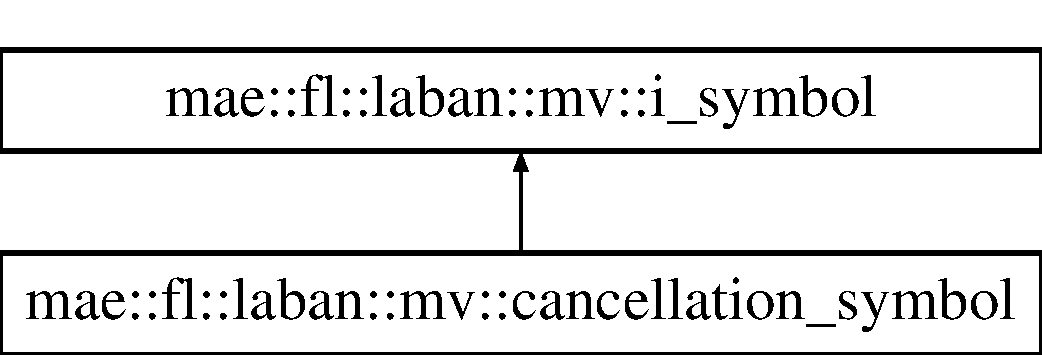
\includegraphics[height=2.000000cm]{classmae_1_1fl_1_1laban_1_1mv_1_1cancellation__symbol}
\end{center}
\end{figure}
\subsection*{Public Member Functions}
\begin{DoxyCompactItemize}
\item 
\hyperlink{classmae_1_1fl_1_1laban_1_1mv_1_1cancellation__symbol_afbf45dbb2de547ac725603b7fb50271b}{cancellation\-\_\-symbol} (e\-\_\-cancel cancel)
\item 
e\-\_\-cancel \hyperlink{classmae_1_1fl_1_1laban_1_1mv_1_1cancellation__symbol_a049928d086d83bb3f8dfec2a4b4c8fbd}{get\-\_\-cancel} () const 
\item 
virtual bool \hyperlink{classmae_1_1fl_1_1laban_1_1mv_1_1cancellation__symbol_a158d3eee246e2e8eda8a8884a209beca}{equals} (std\-::shared\-\_\-ptr$<$ \hyperlink{classmae_1_1fl_1_1laban_1_1mv_1_1i__symbol}{i\-\_\-symbol} $>$ a) const 
\item 
virtual std\-::string \hyperlink{classmae_1_1fl_1_1laban_1_1mv_1_1cancellation__symbol_a17122710f983a1b7308c7103e5e9e222}{xml} (unsigned int indent=0, std\-::string namesp=\char`\"{}\char`\"{}) const 
\item 
virtual std\-::string \hyperlink{classmae_1_1fl_1_1laban_1_1mv_1_1cancellation__symbol_a63cb4ffd49386728f18001301a2b29e3}{svg} (std\-::string identifier, double posx, double posy, double width, double height, bool left=false) const 
\item 
virtual std\-::string \hyperlink{classmae_1_1fl_1_1laban_1_1mv_1_1cancellation__symbol_aa2ff5bbb5398aa454e7995eeb8c1f31a}{str} () const 
\end{DoxyCompactItemize}
\subsection*{Friends}
\begin{DoxyCompactItemize}
\item 
\hypertarget{classmae_1_1fl_1_1laban_1_1mv_1_1cancellation__symbol_af2c0ba97f62f72f8a74aa18eeb192bdc}{std\-::ostream \& {\bfseries operator$<$$<$} (std\-::ostream \&os, const \hyperlink{classmae_1_1fl_1_1laban_1_1mv_1_1cancellation__symbol}{cancellation\-\_\-symbol} \&obj)}\label{classmae_1_1fl_1_1laban_1_1mv_1_1cancellation__symbol_af2c0ba97f62f72f8a74aa18eeb192bdc}

\item 
\hypertarget{classmae_1_1fl_1_1laban_1_1mv_1_1cancellation__symbol_a0a2129bdfd9d4837c5220ab2e22be675}{std\-::ostream \& {\bfseries operator$<$$<$} (std\-::ostream \&os, const std\-::shared\-\_\-ptr$<$ \hyperlink{classmae_1_1fl_1_1laban_1_1mv_1_1cancellation__symbol}{cancellation\-\_\-symbol} $>$ \&obj)}\label{classmae_1_1fl_1_1laban_1_1mv_1_1cancellation__symbol_a0a2129bdfd9d4837c5220ab2e22be675}

\end{DoxyCompactItemize}


\subsection{Constructor \& Destructor Documentation}
\hypertarget{classmae_1_1fl_1_1laban_1_1mv_1_1cancellation__symbol_afbf45dbb2de547ac725603b7fb50271b}{\index{mae\-::fl\-::laban\-::mv\-::cancellation\-\_\-symbol@{mae\-::fl\-::laban\-::mv\-::cancellation\-\_\-symbol}!cancellation\-\_\-symbol@{cancellation\-\_\-symbol}}
\index{cancellation\-\_\-symbol@{cancellation\-\_\-symbol}!mae::fl::laban::mv::cancellation_symbol@{mae\-::fl\-::laban\-::mv\-::cancellation\-\_\-symbol}}
\subsubsection[{cancellation\-\_\-symbol}]{\setlength{\rightskip}{0pt plus 5cm}mae\-::fl\-::laban\-::mv\-::cancellation\-\_\-symbol\-::cancellation\-\_\-symbol (
\begin{DoxyParamCaption}
\item[{e\-\_\-cancel}]{cancel}
\end{DoxyParamCaption}
)}}\label{classmae_1_1fl_1_1laban_1_1mv_1_1cancellation__symbol_afbf45dbb2de547ac725603b7fb50271b}
Creates a cancellation symbol.


\begin{DoxyParams}{Parameters}
{\em cancel} & The cancellation type. \\
\hline
\end{DoxyParams}


\subsection{Member Function Documentation}
\hypertarget{classmae_1_1fl_1_1laban_1_1mv_1_1cancellation__symbol_a158d3eee246e2e8eda8a8884a209beca}{\index{mae\-::fl\-::laban\-::mv\-::cancellation\-\_\-symbol@{mae\-::fl\-::laban\-::mv\-::cancellation\-\_\-symbol}!equals@{equals}}
\index{equals@{equals}!mae::fl::laban::mv::cancellation_symbol@{mae\-::fl\-::laban\-::mv\-::cancellation\-\_\-symbol}}
\subsubsection[{equals}]{\setlength{\rightskip}{0pt plus 5cm}bool mae\-::fl\-::laban\-::mv\-::cancellation\-\_\-symbol\-::equals (
\begin{DoxyParamCaption}
\item[{std\-::shared\-\_\-ptr$<$ {\bf i\-\_\-symbol} $>$}]{a}
\end{DoxyParamCaption}
) const\hspace{0.3cm}{\ttfamily [virtual]}}}\label{classmae_1_1fl_1_1laban_1_1mv_1_1cancellation__symbol_a158d3eee246e2e8eda8a8884a209beca}
Returns true if signs are equal.


\begin{DoxyParams}{Parameters}
{\em a} & The sign to be compared to. \\
\hline
\end{DoxyParams}
\begin{DoxyReturn}{Returns}
True if equal. 
\end{DoxyReturn}


Implements \hyperlink{classmae_1_1fl_1_1laban_1_1mv_1_1i__symbol_a78d90af5e1da4a6561d7545a76689d0e}{mae\-::fl\-::laban\-::mv\-::i\-\_\-symbol}.

\hypertarget{classmae_1_1fl_1_1laban_1_1mv_1_1cancellation__symbol_a049928d086d83bb3f8dfec2a4b4c8fbd}{\index{mae\-::fl\-::laban\-::mv\-::cancellation\-\_\-symbol@{mae\-::fl\-::laban\-::mv\-::cancellation\-\_\-symbol}!get\-\_\-cancel@{get\-\_\-cancel}}
\index{get\-\_\-cancel@{get\-\_\-cancel}!mae::fl::laban::mv::cancellation_symbol@{mae\-::fl\-::laban\-::mv\-::cancellation\-\_\-symbol}}
\subsubsection[{get\-\_\-cancel}]{\setlength{\rightskip}{0pt plus 5cm}e\-\_\-cancel mae\-::fl\-::laban\-::mv\-::cancellation\-\_\-symbol\-::get\-\_\-cancel (
\begin{DoxyParamCaption}
{}
\end{DoxyParamCaption}
) const}}\label{classmae_1_1fl_1_1laban_1_1mv_1_1cancellation__symbol_a049928d086d83bb3f8dfec2a4b4c8fbd}
Returns the cancellation type.

\begin{DoxyReturn}{Returns}
The cancellation type. 
\end{DoxyReturn}
\hypertarget{classmae_1_1fl_1_1laban_1_1mv_1_1cancellation__symbol_aa2ff5bbb5398aa454e7995eeb8c1f31a}{\index{mae\-::fl\-::laban\-::mv\-::cancellation\-\_\-symbol@{mae\-::fl\-::laban\-::mv\-::cancellation\-\_\-symbol}!str@{str}}
\index{str@{str}!mae::fl::laban::mv::cancellation_symbol@{mae\-::fl\-::laban\-::mv\-::cancellation\-\_\-symbol}}
\subsubsection[{str}]{\setlength{\rightskip}{0pt plus 5cm}std\-::string mae\-::fl\-::laban\-::mv\-::cancellation\-\_\-symbol\-::str (
\begin{DoxyParamCaption}
{}
\end{DoxyParamCaption}
) const\hspace{0.3cm}{\ttfamily [virtual]}}}\label{classmae_1_1fl_1_1laban_1_1mv_1_1cancellation__symbol_aa2ff5bbb5398aa454e7995eeb8c1f31a}
Returns the string representation for this element.

\begin{DoxyReturn}{Returns}
The string. 
\end{DoxyReturn}


Implements \hyperlink{classmae_1_1fl_1_1laban_1_1mv_1_1i__symbol_ad254351eabf06ac945c168b24643872e}{mae\-::fl\-::laban\-::mv\-::i\-\_\-symbol}.

\hypertarget{classmae_1_1fl_1_1laban_1_1mv_1_1cancellation__symbol_a63cb4ffd49386728f18001301a2b29e3}{\index{mae\-::fl\-::laban\-::mv\-::cancellation\-\_\-symbol@{mae\-::fl\-::laban\-::mv\-::cancellation\-\_\-symbol}!svg@{svg}}
\index{svg@{svg}!mae::fl::laban::mv::cancellation_symbol@{mae\-::fl\-::laban\-::mv\-::cancellation\-\_\-symbol}}
\subsubsection[{svg}]{\setlength{\rightskip}{0pt plus 5cm}std\-::string mae\-::fl\-::laban\-::mv\-::cancellation\-\_\-symbol\-::svg (
\begin{DoxyParamCaption}
\item[{std\-::string}]{identifier, }
\item[{double}]{posx, }
\item[{double}]{posy, }
\item[{double}]{width, }
\item[{double}]{height, }
\item[{bool}]{left = {\ttfamily false}}
\end{DoxyParamCaption}
) const\hspace{0.3cm}{\ttfamily [virtual]}}}\label{classmae_1_1fl_1_1laban_1_1mv_1_1cancellation__symbol_a63cb4ffd49386728f18001301a2b29e3}
Returns the S\-V\-G representation for this symbol.


\begin{DoxyParams}{Parameters}
{\em posx} & The x position. \\
\hline
{\em posy} & The y position. \\
\hline
{\em width} & The width. \\
\hline
{\em height} & The height. \\
\hline
\end{DoxyParams}
\begin{DoxyReturn}{Returns}
The S\-V\-G. 
\end{DoxyReturn}


Implements \hyperlink{classmae_1_1fl_1_1laban_1_1mv_1_1i__symbol_ae0a724c98c27c05fdde9afff99184029}{mae\-::fl\-::laban\-::mv\-::i\-\_\-symbol}.

\hypertarget{classmae_1_1fl_1_1laban_1_1mv_1_1cancellation__symbol_a17122710f983a1b7308c7103e5e9e222}{\index{mae\-::fl\-::laban\-::mv\-::cancellation\-\_\-symbol@{mae\-::fl\-::laban\-::mv\-::cancellation\-\_\-symbol}!xml@{xml}}
\index{xml@{xml}!mae::fl::laban::mv::cancellation_symbol@{mae\-::fl\-::laban\-::mv\-::cancellation\-\_\-symbol}}
\subsubsection[{xml}]{\setlength{\rightskip}{0pt plus 5cm}std\-::string mae\-::fl\-::laban\-::mv\-::cancellation\-\_\-symbol\-::xml (
\begin{DoxyParamCaption}
\item[{unsigned int}]{indent = {\ttfamily 0}, }
\item[{std\-::string}]{namesp = {\ttfamily \char`\"{}\char`\"{}}}
\end{DoxyParamCaption}
) const\hspace{0.3cm}{\ttfamily [virtual]}}}\label{classmae_1_1fl_1_1laban_1_1mv_1_1cancellation__symbol_a17122710f983a1b7308c7103e5e9e222}
Returns the X\-M\-L representation for this element.


\begin{DoxyParams}{Parameters}
{\em indent} & The applied indent. \\
\hline
{\em namesp} & The prefixed X\-M\-L namespace.\\
\hline
\end{DoxyParams}
\begin{DoxyReturn}{Returns}
The X\-M\-L string. 
\end{DoxyReturn}


Implements \hyperlink{classmae_1_1fl_1_1laban_1_1mv_1_1i__symbol_a05d0b0c74bad854d5e9e3291bbd87b0d}{mae\-::fl\-::laban\-::mv\-::i\-\_\-symbol}.



The documentation for this class was generated from the following files\-:\begin{DoxyCompactItemize}
\item 
src/mae/fl/laban/mv/cancellation\-\_\-symbol.\-hpp\item 
src/mae/fl/laban/mv/cancellation\-\_\-symbol.\-cpp\end{DoxyCompactItemize}

\hypertarget{classmae_1_1fl_1_1laban_1_1column__definition}{\section{mae\-:\-:fl\-:\-:laban\-:\-:column\-\_\-definition Class Reference}
\label{classmae_1_1fl_1_1laban_1_1column__definition}\index{mae\-::fl\-::laban\-::column\-\_\-definition@{mae\-::fl\-::laban\-::column\-\_\-definition}}
}
\subsection*{Public Member Functions}
\begin{DoxyCompactItemize}
\item 
\hyperlink{classmae_1_1fl_1_1laban_1_1column__definition_ac360b410ee99835940cc507ae2bbaf16}{column\-\_\-definition} (int column\-\_\-index, std\-::shared\-\_\-ptr$<$ \hyperlink{classmae_1_1fl_1_1laban_1_1ps_1_1i__pre__sign}{ps\-::i\-\_\-pre\-\_\-sign} $>$ pre\-\_\-sign)
\item 
\hyperlink{classmae_1_1fl_1_1laban_1_1column__definition_a71a931dfbf7c58e098df60269e3985e6}{column\-\_\-definition} (mae\-::e\-\_\-bone eb)
\item 
int \hyperlink{classmae_1_1fl_1_1laban_1_1column__definition_ac4a3d0ea4812adba6a950262bf51dd89}{get\-\_\-column\-\_\-index} () const 
\item 
std\-::shared\-\_\-ptr$<$ \hyperlink{classmae_1_1fl_1_1laban_1_1ps_1_1i__pre__sign}{ps\-::i\-\_\-pre\-\_\-sign} $>$ \hyperlink{classmae_1_1fl_1_1laban_1_1column__definition_abbfe8802f92c4a2d53a7eab415155470}{get\-\_\-pre\-\_\-sign} () const 
\item 
virtual std\-::string \hyperlink{classmae_1_1fl_1_1laban_1_1column__definition_ae159c9be24355b75fcf88c30fa00cf74}{xml} (unsigned int indent=0, std\-::string namesp=\char`\"{}\char`\"{}) const 
\item 
virtual std\-::string \hyperlink{classmae_1_1fl_1_1laban_1_1column__definition_add9bf764a8ca371345ded5f6c006288b}{svg} (unsigned int im\-\_\-width, unsigned int im\-\_\-height, unsigned int max\-\_\-column, unsigned int measures, unsigned int beats\-\_\-per\-\_\-measure) const 
\item 
virtual bool \hyperlink{classmae_1_1fl_1_1laban_1_1column__definition_a48af945f45b023bc78330d0acc8c95c0}{equals} (std\-::shared\-\_\-ptr$<$ \hyperlink{classmae_1_1fl_1_1laban_1_1column__definition}{column\-\_\-definition} $>$ a) const 
\end{DoxyCompactItemize}
\subsection*{Static Public Member Functions}
\begin{DoxyCompactItemize}
\item 
static std\-::vector\\*
$<$ std\-::shared\-\_\-ptr\\*
$<$ \hyperlink{classmae_1_1fl_1_1laban_1_1column__definition}{column\-\_\-definition} $>$ $>$ \hyperlink{classmae_1_1fl_1_1laban_1_1column__definition_a5215ed9abda2085b2829475489b96595}{default\-\_\-definitions} ()
\end{DoxyCompactItemize}


\subsection{Constructor \& Destructor Documentation}
\hypertarget{classmae_1_1fl_1_1laban_1_1column__definition_ac360b410ee99835940cc507ae2bbaf16}{\index{mae\-::fl\-::laban\-::column\-\_\-definition@{mae\-::fl\-::laban\-::column\-\_\-definition}!column\-\_\-definition@{column\-\_\-definition}}
\index{column\-\_\-definition@{column\-\_\-definition}!mae::fl::laban::column_definition@{mae\-::fl\-::laban\-::column\-\_\-definition}}
\subsubsection[{column\-\_\-definition}]{\setlength{\rightskip}{0pt plus 5cm}mae\-::fl\-::laban\-::column\-\_\-definition\-::column\-\_\-definition (
\begin{DoxyParamCaption}
\item[{int}]{column\-\_\-index, }
\item[{std\-::shared\-\_\-ptr$<$ {\bf ps\-::i\-\_\-pre\-\_\-sign} $>$}]{pre\-\_\-sign}
\end{DoxyParamCaption}
)}}\label{classmae_1_1fl_1_1laban_1_1column__definition_ac360b410ee99835940cc507ae2bbaf16}
Creates a new column definition.


\begin{DoxyParams}{Parameters}
{\em column\-\_\-index} & The index of the column. \\
\hline
{\em pre\-\_\-sign} & The pre-\/sign. \\
\hline
\end{DoxyParams}
\hypertarget{classmae_1_1fl_1_1laban_1_1column__definition_a71a931dfbf7c58e098df60269e3985e6}{\index{mae\-::fl\-::laban\-::column\-\_\-definition@{mae\-::fl\-::laban\-::column\-\_\-definition}!column\-\_\-definition@{column\-\_\-definition}}
\index{column\-\_\-definition@{column\-\_\-definition}!mae::fl::laban::column_definition@{mae\-::fl\-::laban\-::column\-\_\-definition}}
\subsubsection[{column\-\_\-definition}]{\setlength{\rightskip}{0pt plus 5cm}mae\-::fl\-::laban\-::column\-\_\-definition\-::column\-\_\-definition (
\begin{DoxyParamCaption}
\item[{mae\-::e\-\_\-bone}]{eb}
\end{DoxyParamCaption}
)}}\label{classmae_1_1fl_1_1laban_1_1column__definition_a71a931dfbf7c58e098df60269e3985e6}
Creates a new column definition for the given e\-\_\-bone enum value.


\begin{DoxyParams}{Parameters}
{\em eb} & The bone enum value. \\
\hline
\end{DoxyParams}


\subsection{Member Function Documentation}
\hypertarget{classmae_1_1fl_1_1laban_1_1column__definition_a5215ed9abda2085b2829475489b96595}{\index{mae\-::fl\-::laban\-::column\-\_\-definition@{mae\-::fl\-::laban\-::column\-\_\-definition}!default\-\_\-definitions@{default\-\_\-definitions}}
\index{default\-\_\-definitions@{default\-\_\-definitions}!mae::fl::laban::column_definition@{mae\-::fl\-::laban\-::column\-\_\-definition}}
\subsubsection[{default\-\_\-definitions}]{\setlength{\rightskip}{0pt plus 5cm}std\-::vector$<$ std\-::shared\-\_\-ptr$<$ {\bf column\-\_\-definition} $>$ $>$ mae\-::fl\-::laban\-::column\-\_\-definition\-::default\-\_\-definitions (
\begin{DoxyParamCaption}
{}
\end{DoxyParamCaption}
)\hspace{0.3cm}{\ttfamily [static]}}}\label{classmae_1_1fl_1_1laban_1_1column__definition_a5215ed9abda2085b2829475489b96595}
Returns the default column definitions.

\begin{DoxyReturn}{Returns}
The default column definitions. 
\end{DoxyReturn}
\hypertarget{classmae_1_1fl_1_1laban_1_1column__definition_a48af945f45b023bc78330d0acc8c95c0}{\index{mae\-::fl\-::laban\-::column\-\_\-definition@{mae\-::fl\-::laban\-::column\-\_\-definition}!equals@{equals}}
\index{equals@{equals}!mae::fl::laban::column_definition@{mae\-::fl\-::laban\-::column\-\_\-definition}}
\subsubsection[{equals}]{\setlength{\rightskip}{0pt plus 5cm}bool mae\-::fl\-::laban\-::column\-\_\-definition\-::equals (
\begin{DoxyParamCaption}
\item[{std\-::shared\-\_\-ptr$<$ {\bf column\-\_\-definition} $>$}]{a}
\end{DoxyParamCaption}
) const\hspace{0.3cm}{\ttfamily [virtual]}}}\label{classmae_1_1fl_1_1laban_1_1column__definition_a48af945f45b023bc78330d0acc8c95c0}
Returns true if signs are equal.


\begin{DoxyParams}{Parameters}
{\em a} & The sign to be compared to. \\
\hline
\end{DoxyParams}
\begin{DoxyReturn}{Returns}
True if equal. 
\end{DoxyReturn}
\hypertarget{classmae_1_1fl_1_1laban_1_1column__definition_ac4a3d0ea4812adba6a950262bf51dd89}{\index{mae\-::fl\-::laban\-::column\-\_\-definition@{mae\-::fl\-::laban\-::column\-\_\-definition}!get\-\_\-column\-\_\-index@{get\-\_\-column\-\_\-index}}
\index{get\-\_\-column\-\_\-index@{get\-\_\-column\-\_\-index}!mae::fl::laban::column_definition@{mae\-::fl\-::laban\-::column\-\_\-definition}}
\subsubsection[{get\-\_\-column\-\_\-index}]{\setlength{\rightskip}{0pt plus 5cm}int mae\-::fl\-::laban\-::column\-\_\-definition\-::get\-\_\-column\-\_\-index (
\begin{DoxyParamCaption}
{}
\end{DoxyParamCaption}
) const}}\label{classmae_1_1fl_1_1laban_1_1column__definition_ac4a3d0ea4812adba6a950262bf51dd89}
Returns the column index. This specifies the addressed column in the chart.

\begin{DoxyReturn}{Returns}

\end{DoxyReturn}
\hypertarget{classmae_1_1fl_1_1laban_1_1column__definition_abbfe8802f92c4a2d53a7eab415155470}{\index{mae\-::fl\-::laban\-::column\-\_\-definition@{mae\-::fl\-::laban\-::column\-\_\-definition}!get\-\_\-pre\-\_\-sign@{get\-\_\-pre\-\_\-sign}}
\index{get\-\_\-pre\-\_\-sign@{get\-\_\-pre\-\_\-sign}!mae::fl::laban::column_definition@{mae\-::fl\-::laban\-::column\-\_\-definition}}
\subsubsection[{get\-\_\-pre\-\_\-sign}]{\setlength{\rightskip}{0pt plus 5cm}std\-::shared\-\_\-ptr$<$ {\bf ps\-::i\-\_\-pre\-\_\-sign} $>$ mae\-::fl\-::laban\-::column\-\_\-definition\-::get\-\_\-pre\-\_\-sign (
\begin{DoxyParamCaption}
{}
\end{DoxyParamCaption}
) const}}\label{classmae_1_1fl_1_1laban_1_1column__definition_abbfe8802f92c4a2d53a7eab415155470}
Returns the pre-\/sign.

\begin{DoxyReturn}{Returns}

\end{DoxyReturn}
\hypertarget{classmae_1_1fl_1_1laban_1_1column__definition_add9bf764a8ca371345ded5f6c006288b}{\index{mae\-::fl\-::laban\-::column\-\_\-definition@{mae\-::fl\-::laban\-::column\-\_\-definition}!svg@{svg}}
\index{svg@{svg}!mae::fl::laban::column_definition@{mae\-::fl\-::laban\-::column\-\_\-definition}}
\subsubsection[{svg}]{\setlength{\rightskip}{0pt plus 5cm}std\-::string mae\-::fl\-::laban\-::column\-\_\-definition\-::svg (
\begin{DoxyParamCaption}
\item[{unsigned int}]{im\-\_\-width, }
\item[{unsigned int}]{im\-\_\-height, }
\item[{unsigned int}]{max\-\_\-column, }
\item[{unsigned int}]{measures, }
\item[{unsigned int}]{beats\-\_\-per\-\_\-measure}
\end{DoxyParamCaption}
) const\hspace{0.3cm}{\ttfamily [virtual]}}}\label{classmae_1_1fl_1_1laban_1_1column__definition_add9bf764a8ca371345ded5f6c006288b}
Returns the S\-V\-G representation for this element.


\begin{DoxyParams}{Parameters}
{\em posx} & The x pos. \\
\hline
{\em posy} & The y pos. \\
\hline
{\em width} & The width. \\
\hline
{\em height} & The height. \\
\hline
\end{DoxyParams}
\begin{DoxyReturn}{Returns}
The S\-V\-G. 
\end{DoxyReturn}
\hypertarget{classmae_1_1fl_1_1laban_1_1column__definition_ae159c9be24355b75fcf88c30fa00cf74}{\index{mae\-::fl\-::laban\-::column\-\_\-definition@{mae\-::fl\-::laban\-::column\-\_\-definition}!xml@{xml}}
\index{xml@{xml}!mae::fl::laban::column_definition@{mae\-::fl\-::laban\-::column\-\_\-definition}}
\subsubsection[{xml}]{\setlength{\rightskip}{0pt plus 5cm}std\-::string mae\-::fl\-::laban\-::column\-\_\-definition\-::xml (
\begin{DoxyParamCaption}
\item[{unsigned int}]{indent = {\ttfamily 0}, }
\item[{std\-::string}]{namesp = {\ttfamily \char`\"{}\char`\"{}}}
\end{DoxyParamCaption}
) const\hspace{0.3cm}{\ttfamily [virtual]}}}\label{classmae_1_1fl_1_1laban_1_1column__definition_ae159c9be24355b75fcf88c30fa00cf74}
Returns the X\-M\-L representation for this element.


\begin{DoxyParams}{Parameters}
{\em indent} & The applied indent. \\
\hline
{\em namesp} & The prefixed X\-M\-L namespace.\\
\hline
\end{DoxyParams}
\begin{DoxyReturn}{Returns}
The X\-M\-L string. 
\end{DoxyReturn}


The documentation for this class was generated from the following files\-:\begin{DoxyCompactItemize}
\item 
src/mae/fl/laban/column\-\_\-definition.\-hpp\item 
src/mae/fl/laban/column\-\_\-definition.\-cpp\end{DoxyCompactItemize}

\hypertarget{classmae_1_1fl_1_1laban_1_1ps_1_1custom__limb}{\section{mae\-:\-:fl\-:\-:laban\-:\-:ps\-:\-:custom\-\_\-limb Class Reference}
\label{classmae_1_1fl_1_1laban_1_1ps_1_1custom__limb}\index{mae\-::fl\-::laban\-::ps\-::custom\-\_\-limb@{mae\-::fl\-::laban\-::ps\-::custom\-\_\-limb}}
}
Inheritance diagram for mae\-:\-:fl\-:\-:laban\-:\-:ps\-:\-:custom\-\_\-limb\-:\begin{figure}[H]
\begin{center}
\leavevmode
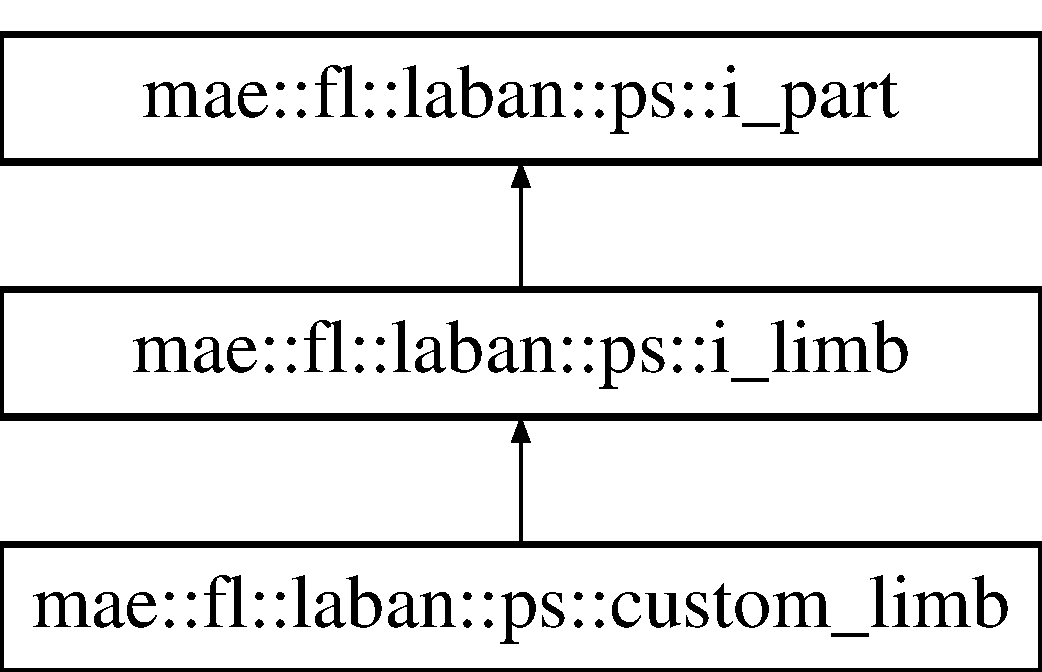
\includegraphics[height=3.000000cm]{classmae_1_1fl_1_1laban_1_1ps_1_1custom__limb}
\end{center}
\end{figure}
\subsection*{Public Member Functions}
\begin{DoxyCompactItemize}
\item 
\hyperlink{classmae_1_1fl_1_1laban_1_1ps_1_1custom__limb_a9c2c37062ecae3f45015afb5c8c7611a}{custom\-\_\-limb} (std\-::shared\-\_\-ptr$<$ \hyperlink{classmae_1_1fl_1_1laban_1_1ps_1_1i__endpoint}{i\-\_\-endpoint} $>$ extremity, std\-::shared\-\_\-ptr$<$ \hyperlink{classmae_1_1fl_1_1laban_1_1ps_1_1i__endpoint}{i\-\_\-endpoint} $>$ fixed\-\_\-end=nullptr)
\item 
std\-::shared\-\_\-ptr$<$ \hyperlink{classmae_1_1fl_1_1laban_1_1ps_1_1i__endpoint}{i\-\_\-endpoint} $>$ \hyperlink{classmae_1_1fl_1_1laban_1_1ps_1_1custom__limb_a5714efb1c984f1b9a4b6d086627266c9}{get\-\_\-fixed\-\_\-end} () const 
\item 
std\-::shared\-\_\-ptr$<$ \hyperlink{classmae_1_1fl_1_1laban_1_1ps_1_1i__endpoint}{i\-\_\-endpoint} $>$ \hyperlink{classmae_1_1fl_1_1laban_1_1ps_1_1custom__limb_ade139b5ffa96d4b61f40fcea26e3d200}{get\-\_\-extremity} () const 
\item 
virtual std\-::string \hyperlink{classmae_1_1fl_1_1laban_1_1ps_1_1custom__limb_a2622dd693ce2f662a4802025b42f1e64}{xml} (unsigned int indent=0, std\-::string namesp=\char`\"{}\char`\"{}) const 
\item 
virtual std\-::string \hyperlink{classmae_1_1fl_1_1laban_1_1ps_1_1custom__limb_aa002dfaca3b1f073f67a85572095b504}{svg} (std\-::string identifier, double posx, double posy, double width, double height, bool left=false) const 
\item 
virtual bool \hyperlink{classmae_1_1fl_1_1laban_1_1ps_1_1custom__limb_aea87a1c04a4a8fde3ef80862690b0318}{equals} (std\-::shared\-\_\-ptr$<$ \hyperlink{classmae_1_1fl_1_1laban_1_1ps_1_1i__part}{i\-\_\-part} $>$ a) const 
\item 
virtual bool \hyperlink{classmae_1_1fl_1_1laban_1_1ps_1_1custom__limb_ab152826ff0de843c52695807715a6c71}{equals} (std\-::shared\-\_\-ptr$<$ \hyperlink{classmae_1_1fl_1_1laban_1_1ps_1_1i__limb}{i\-\_\-limb} $>$ a) const 
\end{DoxyCompactItemize}


\subsection{Constructor \& Destructor Documentation}
\hypertarget{classmae_1_1fl_1_1laban_1_1ps_1_1custom__limb_a9c2c37062ecae3f45015afb5c8c7611a}{\index{mae\-::fl\-::laban\-::ps\-::custom\-\_\-limb@{mae\-::fl\-::laban\-::ps\-::custom\-\_\-limb}!custom\-\_\-limb@{custom\-\_\-limb}}
\index{custom\-\_\-limb@{custom\-\_\-limb}!mae::fl::laban::ps::custom_limb@{mae\-::fl\-::laban\-::ps\-::custom\-\_\-limb}}
\subsubsection[{custom\-\_\-limb}]{\setlength{\rightskip}{0pt plus 5cm}mae\-::fl\-::laban\-::ps\-::custom\-\_\-limb\-::custom\-\_\-limb (
\begin{DoxyParamCaption}
\item[{std\-::shared\-\_\-ptr$<$ {\bf i\-\_\-endpoint} $>$}]{extremity, }
\item[{std\-::shared\-\_\-ptr$<$ {\bf i\-\_\-endpoint} $>$}]{fixed\-\_\-end = {\ttfamily nullptr}}
\end{DoxyParamCaption}
)}}\label{classmae_1_1fl_1_1laban_1_1ps_1_1custom__limb_a9c2c37062ecae3f45015afb5c8c7611a}
Creates a custom limb pre-\/sign which is defined as the limb between two endpoints.


\begin{DoxyParams}{Parameters}
{\em fixed\-\_\-end} & The fixed end of the limb. \\
\hline
{\em extremity} & (optional) The extremity end of the limb. \\
\hline
\end{DoxyParams}


\subsection{Member Function Documentation}
\hypertarget{classmae_1_1fl_1_1laban_1_1ps_1_1custom__limb_aea87a1c04a4a8fde3ef80862690b0318}{\index{mae\-::fl\-::laban\-::ps\-::custom\-\_\-limb@{mae\-::fl\-::laban\-::ps\-::custom\-\_\-limb}!equals@{equals}}
\index{equals@{equals}!mae::fl::laban::ps::custom_limb@{mae\-::fl\-::laban\-::ps\-::custom\-\_\-limb}}
\subsubsection[{equals}]{\setlength{\rightskip}{0pt plus 5cm}bool mae\-::fl\-::laban\-::ps\-::custom\-\_\-limb\-::equals (
\begin{DoxyParamCaption}
\item[{std\-::shared\-\_\-ptr$<$ {\bf i\-\_\-part} $>$}]{a}
\end{DoxyParamCaption}
) const\hspace{0.3cm}{\ttfamily [virtual]}}}\label{classmae_1_1fl_1_1laban_1_1ps_1_1custom__limb_aea87a1c04a4a8fde3ef80862690b0318}
Returns true if elements are equal.


\begin{DoxyParams}{Parameters}
{\em a} & The element to be compared to. \\
\hline
\end{DoxyParams}
\begin{DoxyReturn}{Returns}
True if equal. 
\end{DoxyReturn}


Implements \hyperlink{classmae_1_1fl_1_1laban_1_1ps_1_1i__limb_aa46cb4b952cc2a8692f3f32895a28041}{mae\-::fl\-::laban\-::ps\-::i\-\_\-limb}.

\hypertarget{classmae_1_1fl_1_1laban_1_1ps_1_1custom__limb_ab152826ff0de843c52695807715a6c71}{\index{mae\-::fl\-::laban\-::ps\-::custom\-\_\-limb@{mae\-::fl\-::laban\-::ps\-::custom\-\_\-limb}!equals@{equals}}
\index{equals@{equals}!mae::fl::laban::ps::custom_limb@{mae\-::fl\-::laban\-::ps\-::custom\-\_\-limb}}
\subsubsection[{equals}]{\setlength{\rightskip}{0pt plus 5cm}bool mae\-::fl\-::laban\-::ps\-::custom\-\_\-limb\-::equals (
\begin{DoxyParamCaption}
\item[{std\-::shared\-\_\-ptr$<$ {\bf i\-\_\-limb} $>$}]{a}
\end{DoxyParamCaption}
) const\hspace{0.3cm}{\ttfamily [virtual]}}}\label{classmae_1_1fl_1_1laban_1_1ps_1_1custom__limb_ab152826ff0de843c52695807715a6c71}
Returns true if elements are equal.


\begin{DoxyParams}{Parameters}
{\em a} & The element to be compared to. \\
\hline
\end{DoxyParams}
\begin{DoxyReturn}{Returns}
True if equal. 
\end{DoxyReturn}


Implements \hyperlink{classmae_1_1fl_1_1laban_1_1ps_1_1i__limb_a7e7ba568e9711b8901234f2cb73b67b8}{mae\-::fl\-::laban\-::ps\-::i\-\_\-limb}.

\hypertarget{classmae_1_1fl_1_1laban_1_1ps_1_1custom__limb_ade139b5ffa96d4b61f40fcea26e3d200}{\index{mae\-::fl\-::laban\-::ps\-::custom\-\_\-limb@{mae\-::fl\-::laban\-::ps\-::custom\-\_\-limb}!get\-\_\-extremity@{get\-\_\-extremity}}
\index{get\-\_\-extremity@{get\-\_\-extremity}!mae::fl::laban::ps::custom_limb@{mae\-::fl\-::laban\-::ps\-::custom\-\_\-limb}}
\subsubsection[{get\-\_\-extremity}]{\setlength{\rightskip}{0pt plus 5cm}std\-::shared\-\_\-ptr$<$ {\bf i\-\_\-endpoint} $>$ mae\-::fl\-::laban\-::ps\-::custom\-\_\-limb\-::get\-\_\-extremity (
\begin{DoxyParamCaption}
{}
\end{DoxyParamCaption}
) const}}\label{classmae_1_1fl_1_1laban_1_1ps_1_1custom__limb_ade139b5ffa96d4b61f40fcea26e3d200}
Returns the extremity end of the limb if set. Returns null otherwise.

\begin{DoxyReturn}{Returns}

\end{DoxyReturn}
\hypertarget{classmae_1_1fl_1_1laban_1_1ps_1_1custom__limb_a5714efb1c984f1b9a4b6d086627266c9}{\index{mae\-::fl\-::laban\-::ps\-::custom\-\_\-limb@{mae\-::fl\-::laban\-::ps\-::custom\-\_\-limb}!get\-\_\-fixed\-\_\-end@{get\-\_\-fixed\-\_\-end}}
\index{get\-\_\-fixed\-\_\-end@{get\-\_\-fixed\-\_\-end}!mae::fl::laban::ps::custom_limb@{mae\-::fl\-::laban\-::ps\-::custom\-\_\-limb}}
\subsubsection[{get\-\_\-fixed\-\_\-end}]{\setlength{\rightskip}{0pt plus 5cm}std\-::shared\-\_\-ptr$<$ {\bf i\-\_\-endpoint} $>$ mae\-::fl\-::laban\-::ps\-::custom\-\_\-limb\-::get\-\_\-fixed\-\_\-end (
\begin{DoxyParamCaption}
{}
\end{DoxyParamCaption}
) const}}\label{classmae_1_1fl_1_1laban_1_1ps_1_1custom__limb_a5714efb1c984f1b9a4b6d086627266c9}
Returns the fixed end of the limb.

\begin{DoxyReturn}{Returns}

\end{DoxyReturn}
\hypertarget{classmae_1_1fl_1_1laban_1_1ps_1_1custom__limb_aa002dfaca3b1f073f67a85572095b504}{\index{mae\-::fl\-::laban\-::ps\-::custom\-\_\-limb@{mae\-::fl\-::laban\-::ps\-::custom\-\_\-limb}!svg@{svg}}
\index{svg@{svg}!mae::fl::laban::ps::custom_limb@{mae\-::fl\-::laban\-::ps\-::custom\-\_\-limb}}
\subsubsection[{svg}]{\setlength{\rightskip}{0pt plus 5cm}std\-::string mae\-::fl\-::laban\-::ps\-::custom\-\_\-limb\-::svg (
\begin{DoxyParamCaption}
\item[{std\-::string}]{identifier, }
\item[{double}]{posx, }
\item[{double}]{posy, }
\item[{double}]{width, }
\item[{double}]{height, }
\item[{bool}]{left = {\ttfamily false}}
\end{DoxyParamCaption}
) const\hspace{0.3cm}{\ttfamily [virtual]}}}\label{classmae_1_1fl_1_1laban_1_1ps_1_1custom__limb_aa002dfaca3b1f073f67a85572095b504}
Returns the S\-V\-G representation for this symbol.


\begin{DoxyParams}{Parameters}
{\em posx} & The x position. \\
\hline
{\em posy} & The y position. \\
\hline
{\em width} & The width. \\
\hline
{\em height} & The height. \\
\hline
\end{DoxyParams}
\begin{DoxyReturn}{Returns}
The S\-V\-G. 
\end{DoxyReturn}


Implements \hyperlink{classmae_1_1fl_1_1laban_1_1ps_1_1i__part_a78227d5ecd87655a7a9454c68f470368}{mae\-::fl\-::laban\-::ps\-::i\-\_\-part}.

\hypertarget{classmae_1_1fl_1_1laban_1_1ps_1_1custom__limb_a2622dd693ce2f662a4802025b42f1e64}{\index{mae\-::fl\-::laban\-::ps\-::custom\-\_\-limb@{mae\-::fl\-::laban\-::ps\-::custom\-\_\-limb}!xml@{xml}}
\index{xml@{xml}!mae::fl::laban::ps::custom_limb@{mae\-::fl\-::laban\-::ps\-::custom\-\_\-limb}}
\subsubsection[{xml}]{\setlength{\rightskip}{0pt plus 5cm}std\-::string mae\-::fl\-::laban\-::ps\-::custom\-\_\-limb\-::xml (
\begin{DoxyParamCaption}
\item[{unsigned int}]{indent = {\ttfamily 0}, }
\item[{std\-::string}]{namesp = {\ttfamily \char`\"{}\char`\"{}}}
\end{DoxyParamCaption}
) const\hspace{0.3cm}{\ttfamily [virtual]}}}\label{classmae_1_1fl_1_1laban_1_1ps_1_1custom__limb_a2622dd693ce2f662a4802025b42f1e64}
Returns the X\-M\-L representation for this element.


\begin{DoxyParams}{Parameters}
{\em indent} & The applied indent. \\
\hline
{\em namesp} & The prefixed X\-M\-L namespace.\\
\hline
\end{DoxyParams}
\begin{DoxyReturn}{Returns}
The X\-M\-L string. 
\end{DoxyReturn}


Implements \hyperlink{classmae_1_1fl_1_1laban_1_1ps_1_1i__limb_a7a5c3ca32936748a1e60fdab1d29b1c9}{mae\-::fl\-::laban\-::ps\-::i\-\_\-limb}.



The documentation for this class was generated from the following files\-:\begin{DoxyCompactItemize}
\item 
src/mae/fl/laban/ps/custom\-\_\-limb.\-hpp\item 
src/mae/fl/laban/ps/custom\-\_\-limb.\-cpp\end{DoxyCompactItemize}

\hypertarget{classmae_1_1fl_1_1laban_1_1decision__forest}{\section{mae\-:\-:fl\-:\-:laban\-:\-:decision\-\_\-forest Class Reference}
\label{classmae_1_1fl_1_1laban_1_1decision__forest}\index{mae\-::fl\-::laban\-::decision\-\_\-forest@{mae\-::fl\-::laban\-::decision\-\_\-forest}}
}
\subsection*{Public Member Functions}
\begin{DoxyCompactItemize}
\item 
\hyperlink{classmae_1_1fl_1_1laban_1_1decision__forest_af04ed42b665c58b4ba3aa7248e0be0a8}{decision\-\_\-forest} (std\-::vector$<$ std\-::shared\-\_\-ptr$<$ \hyperlink{classmae_1_1fl_1_1laban_1_1column__definition}{column\-\_\-definition} $>$ $>$ column\-\_\-definitions=std\-::vector$<$ std\-::shared\-\_\-ptr$<$ \hyperlink{classmae_1_1fl_1_1laban_1_1column__definition}{column\-\_\-definition} $>$ $>$(), std\-::vector$<$ int $>$ reserved\-\_\-columns=\hyperlink{classmae_1_1fl_1_1laban_1_1laban__sequence_adda43b657712484d90b4ef3927a81128}{laban\-\_\-sequence\-::default\-\_\-columns}(), unsigned int beats\-\_\-per\-\_\-measure=\hyperlink{classmae_1_1fl_1_1laban_1_1laban__sequence_a2e64362d5cfeb89eb8545cb064e63170}{laban\-\_\-sequence\-::default\-\_\-beats\-\_\-per\-\_\-measure}(), unsigned int beat\-\_\-duration=\hyperlink{classmae_1_1fl_1_1laban_1_1laban__sequence_ac7bf04cdac0c3aed6b8ee4a887e561d9}{laban\-\_\-sequence\-::default\-\_\-beat\-\_\-duration}(), e\-\_\-time\-\_\-unit time\-\_\-unit=\hyperlink{classmae_1_1fl_1_1laban_1_1laban__sequence_ada28215d43d85e983fe6129e9816eed2}{laban\-\_\-sequence\-::default\-\_\-time\-\_\-unit}(), std\-::shared\-\_\-ptr$<$ \hyperlink{classmae_1_1fl_1_1laban_1_1i__decision__maker}{i\-\_\-decision\-\_\-maker}$<$ \hyperlink{classmae_1_1fl_1_1laban_1_1i__movement}{i\-\_\-movement} $>$ $>$ dec\-\_\-maker=nullptr, std\-::shared\-\_\-ptr$<$ \hyperlink{classmae_1_1fl_1_1laban_1_1rewriting__forest}{rewriting\-\_\-forest} $>$ rw=nullptr)
\item 
virtual void \hyperlink{classmae_1_1fl_1_1laban_1_1decision__forest_a7308f844dea15ccb31b7c85529388c04}{set\-\_\-recognition\-\_\-tolerance} (double tolerance)
\item 
virtual void \hyperlink{classmae_1_1fl_1_1laban_1_1decision__forest_a4794a8981cd0cfeb55a00ec6a5d01edf}{add\-\_\-sequence} (std\-::shared\-\_\-ptr$<$ \hyperlink{classmae_1_1fl_1_1laban_1_1laban__sequence}{laban\-\_\-sequence} $>$ sequence)
\item 
virtual bool \hyperlink{classmae_1_1fl_1_1laban_1_1decision__forest_a24a8f97645622dbd96543763821dc6e5}{remove\-\_\-sequence} (std\-::shared\-\_\-ptr$<$ \hyperlink{classmae_1_1fl_1_1laban_1_1laban__sequence}{laban\-\_\-sequence} $>$ sequence)
\item 
virtual bool \hyperlink{classmae_1_1fl_1_1laban_1_1decision__forest_a41951d257154b85832f3d6beea13d4e6}{remove\-\_\-sequence} (unsigned int list\-\_\-index)
\item 
virtual void \hyperlink{classmae_1_1fl_1_1laban_1_1decision__forest_aa623f14cda0e8d9566716be9bd6f74d4}{clear} ()
\item 
virtual void \hyperlink{classmae_1_1fl_1_1laban_1_1decision__forest_a639c688ff26b2ecf20f30ae731d7f44f}{add\-\_\-rewriting\-\_\-rule} (std\-::vector$<$ std\-::shared\-\_\-ptr$<$ \hyperlink{classmae_1_1fl_1_1laban_1_1i__movement}{i\-\_\-movement} $>$ $>$ sequence, std\-::shared\-\_\-ptr$<$ std\-::vector$<$ std\-::vector$<$ std\-::shared\-\_\-ptr$<$ \hyperlink{classmae_1_1fl_1_1laban_1_1i__movement}{i\-\_\-movement} $>$ $>$ $>$ $>$ replacements)
\item 
virtual void \hyperlink{classmae_1_1fl_1_1laban_1_1decision__forest_a967fa135b60859542d073b1df27e39c8}{add\-\_\-rewriting\-\_\-rule} (std\-::shared\-\_\-ptr$<$ \hyperlink{classmae_1_1fl_1_1laban_1_1decision__value}{decision\-\_\-value}$<$ \hyperlink{classmae_1_1fl_1_1laban_1_1i__movement}{i\-\_\-movement}, std\-::vector$<$ std\-::vector$<$ std\-::shared\-\_\-ptr$<$ \hyperlink{classmae_1_1fl_1_1laban_1_1i__movement}{i\-\_\-movement} $>$ $>$ $>$ $>$ $>$ rule)
\item 
std\-::shared\-\_\-ptr$<$ \hyperlink{classmae_1_1fl_1_1laban_1_1laban__sequence}{laban\-\_\-sequence} $>$ \hyperlink{classmae_1_1fl_1_1laban_1_1decision__forest_ab295e95474c126e9f61c67897bc456f5}{recreate\-\_\-sequence} (std\-::shared\-\_\-ptr$<$ \hyperlink{classmae_1_1fl_1_1laban_1_1laban__sequence}{laban\-\_\-sequence} $>$ sequence)
\item 
virtual std\-::list\\*
$<$ std\-::shared\-\_\-ptr\\*
$<$ \hyperlink{classmae_1_1fl_1_1laban_1_1laban__sequence}{laban\-\_\-sequence} $>$ $>$ \hyperlink{classmae_1_1fl_1_1laban_1_1decision__forest_a023111c5a44a950677d99412b4bad7d2}{get\-\_\-sequences} ()
\item 
virtual std\-::vector\\*
$<$ std\-::shared\-\_\-ptr\\*
$<$ \hyperlink{classmae_1_1fl_1_1laban_1_1laban__sequence}{laban\-\_\-sequence} $>$ $>$ \hyperlink{classmae_1_1fl_1_1laban_1_1decision__forest_a8516b4336ab69541927a9f2d2f4f0d85}{find\-\_\-submatches} (std\-::shared\-\_\-ptr$<$ \hyperlink{classmae_1_1fl_1_1laban_1_1laban__sequence}{laban\-\_\-sequence} $>$ whole\-\_\-sequence, std\-::vector$<$ \hyperlink{classmae_1_1bone}{bone} $>$ body\-\_\-parts)
\item 
virtual std\-::string \hyperlink{classmae_1_1fl_1_1laban_1_1decision__forest_a23977c20fd4923e0cb4da1ba380821c3}{str} ()
\end{DoxyCompactItemize}


\subsection{Constructor \& Destructor Documentation}
\hypertarget{classmae_1_1fl_1_1laban_1_1decision__forest_af04ed42b665c58b4ba3aa7248e0be0a8}{\index{mae\-::fl\-::laban\-::decision\-\_\-forest@{mae\-::fl\-::laban\-::decision\-\_\-forest}!decision\-\_\-forest@{decision\-\_\-forest}}
\index{decision\-\_\-forest@{decision\-\_\-forest}!mae::fl::laban::decision_forest@{mae\-::fl\-::laban\-::decision\-\_\-forest}}
\subsubsection[{decision\-\_\-forest}]{\setlength{\rightskip}{0pt plus 5cm}mae\-::fl\-::laban\-::decision\-\_\-forest\-::decision\-\_\-forest (
\begin{DoxyParamCaption}
\item[{std\-::vector$<$ std\-::shared\-\_\-ptr$<$ {\bf column\-\_\-definition} $>$ $>$}]{column\-\_\-definitions = {\ttfamily std\-:\-:vector$<$~std\-:\-:shared\-\_\-ptr$<${\bf column\-\_\-definition}$>$~$>$()}, }
\item[{std\-::vector$<$ int $>$}]{reserved\-\_\-columns = {\ttfamily {\bf laban\-\_\-sequence\-::default\-\_\-columns}()}, }
\item[{unsigned int}]{beats\-\_\-per\-\_\-measure = {\ttfamily {\bf laban\-\_\-sequence\-::default\-\_\-beats\-\_\-per\-\_\-measure}()}, }
\item[{unsigned int}]{beat\-\_\-duration = {\ttfamily {\bf laban\-\_\-sequence\-::default\-\_\-beat\-\_\-duration}()}, }
\item[{e\-\_\-time\-\_\-unit}]{time\-\_\-unit = {\ttfamily {\bf laban\-\_\-sequence\-::default\-\_\-time\-\_\-unit}()}, }
\item[{std\-::shared\-\_\-ptr$<$ {\bf i\-\_\-decision\-\_\-maker}$<$ {\bf i\-\_\-movement} $>$ $>$}]{dec\-\_\-maker = {\ttfamily nullptr}, }
\item[{std\-::shared\-\_\-ptr$<$ {\bf rewriting\-\_\-forest} $>$}]{rw = {\ttfamily nullptr}}
\end{DoxyParamCaption}
)}}\label{classmae_1_1fl_1_1laban_1_1decision__forest_af04ed42b665c58b4ba3aa7248e0be0a8}
Creates a new decision forest for laban\-\_\-sequences.


\begin{DoxyParams}{Parameters}
{\em column\-\_\-definitions} & The columns that are taken into account (besides the default ones). \\
\hline
{\em reserved\-\_\-columns} & The reserved columns used by the scores. \\
\hline
{\em beats\-\_\-per\-\_\-measure} & The number of beats per measure. \\
\hline
{\em beat\-\_\-duration} & The duration of a single beat. \\
\hline
{\em time\-\_\-unit} & The time unit used by the scores. \\
\hline
{\em dec\-\_\-maker} & The decision maker to compare movements. \\
\hline
{\em rw} & The rewriting forest. If not set not rewriting rules are applied. \\
\hline
\end{DoxyParams}


\subsection{Member Function Documentation}
\hypertarget{classmae_1_1fl_1_1laban_1_1decision__forest_a639c688ff26b2ecf20f30ae731d7f44f}{\index{mae\-::fl\-::laban\-::decision\-\_\-forest@{mae\-::fl\-::laban\-::decision\-\_\-forest}!add\-\_\-rewriting\-\_\-rule@{add\-\_\-rewriting\-\_\-rule}}
\index{add\-\_\-rewriting\-\_\-rule@{add\-\_\-rewriting\-\_\-rule}!mae::fl::laban::decision_forest@{mae\-::fl\-::laban\-::decision\-\_\-forest}}
\subsubsection[{add\-\_\-rewriting\-\_\-rule}]{\setlength{\rightskip}{0pt plus 5cm}void mae\-::fl\-::laban\-::decision\-\_\-forest\-::add\-\_\-rewriting\-\_\-rule (
\begin{DoxyParamCaption}
\item[{std\-::vector$<$ std\-::shared\-\_\-ptr$<$ {\bf i\-\_\-movement} $>$ $>$}]{sequence, }
\item[{std\-::shared\-\_\-ptr$<$ std\-::vector$<$ std\-::vector$<$ std\-::shared\-\_\-ptr$<$ {\bf i\-\_\-movement} $>$ $>$ $>$ $>$}]{replacements}
\end{DoxyParamCaption}
)\hspace{0.3cm}{\ttfamily [virtual]}}}\label{classmae_1_1fl_1_1laban_1_1decision__forest_a639c688ff26b2ecf20f30ae731d7f44f}
Adds a rewriting rule to the forest.


\begin{DoxyParams}{Parameters}
{\em sequence} & The sequence. \\
\hline
{\em replacements} & The replacement for the sequence. \\
\hline
\end{DoxyParams}
\hypertarget{classmae_1_1fl_1_1laban_1_1decision__forest_a967fa135b60859542d073b1df27e39c8}{\index{mae\-::fl\-::laban\-::decision\-\_\-forest@{mae\-::fl\-::laban\-::decision\-\_\-forest}!add\-\_\-rewriting\-\_\-rule@{add\-\_\-rewriting\-\_\-rule}}
\index{add\-\_\-rewriting\-\_\-rule@{add\-\_\-rewriting\-\_\-rule}!mae::fl::laban::decision_forest@{mae\-::fl\-::laban\-::decision\-\_\-forest}}
\subsubsection[{add\-\_\-rewriting\-\_\-rule}]{\setlength{\rightskip}{0pt plus 5cm}void mae\-::fl\-::laban\-::decision\-\_\-forest\-::add\-\_\-rewriting\-\_\-rule (
\begin{DoxyParamCaption}
\item[{std\-::shared\-\_\-ptr$<$ {\bf decision\-\_\-value}$<$ {\bf i\-\_\-movement}, std\-::vector$<$ std\-::vector$<$ std\-::shared\-\_\-ptr$<$ {\bf i\-\_\-movement} $>$ $>$ $>$ $>$ $>$}]{rule}
\end{DoxyParamCaption}
)\hspace{0.3cm}{\ttfamily [virtual]}}}\label{classmae_1_1fl_1_1laban_1_1decision__forest_a967fa135b60859542d073b1df27e39c8}
Adds a rewriting rule to the forest.


\begin{DoxyParams}{Parameters}
{\em rule} & The rule to be added. \\
\hline
\end{DoxyParams}
\hypertarget{classmae_1_1fl_1_1laban_1_1decision__forest_a4794a8981cd0cfeb55a00ec6a5d01edf}{\index{mae\-::fl\-::laban\-::decision\-\_\-forest@{mae\-::fl\-::laban\-::decision\-\_\-forest}!add\-\_\-sequence@{add\-\_\-sequence}}
\index{add\-\_\-sequence@{add\-\_\-sequence}!mae::fl::laban::decision_forest@{mae\-::fl\-::laban\-::decision\-\_\-forest}}
\subsubsection[{add\-\_\-sequence}]{\setlength{\rightskip}{0pt plus 5cm}void mae\-::fl\-::laban\-::decision\-\_\-forest\-::add\-\_\-sequence (
\begin{DoxyParamCaption}
\item[{std\-::shared\-\_\-ptr$<$ {\bf laban\-\_\-sequence} $>$}]{sequence}
\end{DoxyParamCaption}
)\hspace{0.3cm}{\ttfamily [virtual]}}}\label{classmae_1_1fl_1_1laban_1_1decision__forest_a4794a8981cd0cfeb55a00ec6a5d01edf}
Adds a sequence to the forest. It will stored in different decision trees for each body part. Since body part I\-Ds are used to identify the columns, the column definition for all sequences should be the same.


\begin{DoxyParams}{Parameters}
{\em sequence} & The sequence to be registered. \\
\hline
\end{DoxyParams}
\hypertarget{classmae_1_1fl_1_1laban_1_1decision__forest_aa623f14cda0e8d9566716be9bd6f74d4}{\index{mae\-::fl\-::laban\-::decision\-\_\-forest@{mae\-::fl\-::laban\-::decision\-\_\-forest}!clear@{clear}}
\index{clear@{clear}!mae::fl::laban::decision_forest@{mae\-::fl\-::laban\-::decision\-\_\-forest}}
\subsubsection[{clear}]{\setlength{\rightskip}{0pt plus 5cm}void mae\-::fl\-::laban\-::decision\-\_\-forest\-::clear (
\begin{DoxyParamCaption}
{}
\end{DoxyParamCaption}
)\hspace{0.3cm}{\ttfamily [virtual]}}}\label{classmae_1_1fl_1_1laban_1_1decision__forest_aa623f14cda0e8d9566716be9bd6f74d4}
Removes all sequences from the forest. This removes all associated trees either. \hypertarget{classmae_1_1fl_1_1laban_1_1decision__forest_a8516b4336ab69541927a9f2d2f4f0d85}{\index{mae\-::fl\-::laban\-::decision\-\_\-forest@{mae\-::fl\-::laban\-::decision\-\_\-forest}!find\-\_\-submatches@{find\-\_\-submatches}}
\index{find\-\_\-submatches@{find\-\_\-submatches}!mae::fl::laban::decision_forest@{mae\-::fl\-::laban\-::decision\-\_\-forest}}
\subsubsection[{find\-\_\-submatches}]{\setlength{\rightskip}{0pt plus 5cm}std\-::vector$<$ std\-::shared\-\_\-ptr$<$ {\bf laban\-\_\-sequence} $>$ $>$ mae\-::fl\-::laban\-::decision\-\_\-forest\-::find\-\_\-submatches (
\begin{DoxyParamCaption}
\item[{std\-::shared\-\_\-ptr$<$ {\bf laban\-\_\-sequence} $>$}]{whole\-\_\-sequence, }
\item[{std\-::vector$<$ {\bf bone} $>$}]{body\-\_\-parts}
\end{DoxyParamCaption}
)\hspace{0.3cm}{\ttfamily [virtual]}}}\label{classmae_1_1fl_1_1laban_1_1decision__forest_a8516b4336ab69541927a9f2d2f4f0d85}
Searches the sequence for matches of subsequences (which are the registered ones).


\begin{DoxyParams}{Parameters}
{\em whole\-\_\-sequence} & The whole sequence to be processed. \\
\hline
{\em body\-\_\-parts} & All the body parts that are meant to be taken into account. \\
\hline
\end{DoxyParams}
\begin{DoxyReturn}{Returns}
All matching sequences. 
\end{DoxyReturn}
\hypertarget{classmae_1_1fl_1_1laban_1_1decision__forest_a023111c5a44a950677d99412b4bad7d2}{\index{mae\-::fl\-::laban\-::decision\-\_\-forest@{mae\-::fl\-::laban\-::decision\-\_\-forest}!get\-\_\-sequences@{get\-\_\-sequences}}
\index{get\-\_\-sequences@{get\-\_\-sequences}!mae::fl::laban::decision_forest@{mae\-::fl\-::laban\-::decision\-\_\-forest}}
\subsubsection[{get\-\_\-sequences}]{\setlength{\rightskip}{0pt plus 5cm}std\-::list$<$ std\-::shared\-\_\-ptr$<$ {\bf laban\-\_\-sequence} $>$ $>$ mae\-::fl\-::laban\-::decision\-\_\-forest\-::get\-\_\-sequences (
\begin{DoxyParamCaption}
{}
\end{DoxyParamCaption}
)\hspace{0.3cm}{\ttfamily [virtual]}}}\label{classmae_1_1fl_1_1laban_1_1decision__forest_a023111c5a44a950677d99412b4bad7d2}
Returns all registered sequences.

\begin{DoxyReturn}{Returns}
All sequences. 
\end{DoxyReturn}
\hypertarget{classmae_1_1fl_1_1laban_1_1decision__forest_ab295e95474c126e9f61c67897bc456f5}{\index{mae\-::fl\-::laban\-::decision\-\_\-forest@{mae\-::fl\-::laban\-::decision\-\_\-forest}!recreate\-\_\-sequence@{recreate\-\_\-sequence}}
\index{recreate\-\_\-sequence@{recreate\-\_\-sequence}!mae::fl::laban::decision_forest@{mae\-::fl\-::laban\-::decision\-\_\-forest}}
\subsubsection[{recreate\-\_\-sequence}]{\setlength{\rightskip}{0pt plus 5cm}std\-::shared\-\_\-ptr$<$ {\bf laban\-\_\-sequence} $>$ mae\-::fl\-::laban\-::decision\-\_\-forest\-::recreate\-\_\-sequence (
\begin{DoxyParamCaption}
\item[{std\-::shared\-\_\-ptr$<$ {\bf laban\-\_\-sequence} $>$}]{sequence}
\end{DoxyParamCaption}
)}}\label{classmae_1_1fl_1_1laban_1_1decision__forest_ab295e95474c126e9f61c67897bc456f5}
Recreates the sequence with adjusted beat duration, beats per measure and time unit. Additionally the column definitions are adjusted.


\begin{DoxyParams}{Parameters}
{\em sequence} & The sequence to be recreated. \\
\hline
\end{DoxyParams}
\begin{DoxyReturn}{Returns}
The new, adjusted sequence. 
\end{DoxyReturn}
\hypertarget{classmae_1_1fl_1_1laban_1_1decision__forest_a24a8f97645622dbd96543763821dc6e5}{\index{mae\-::fl\-::laban\-::decision\-\_\-forest@{mae\-::fl\-::laban\-::decision\-\_\-forest}!remove\-\_\-sequence@{remove\-\_\-sequence}}
\index{remove\-\_\-sequence@{remove\-\_\-sequence}!mae::fl::laban::decision_forest@{mae\-::fl\-::laban\-::decision\-\_\-forest}}
\subsubsection[{remove\-\_\-sequence}]{\setlength{\rightskip}{0pt plus 5cm}bool mae\-::fl\-::laban\-::decision\-\_\-forest\-::remove\-\_\-sequence (
\begin{DoxyParamCaption}
\item[{std\-::shared\-\_\-ptr$<$ {\bf laban\-\_\-sequence} $>$}]{sequence}
\end{DoxyParamCaption}
)\hspace{0.3cm}{\ttfamily [virtual]}}}\label{classmae_1_1fl_1_1laban_1_1decision__forest_a24a8f97645622dbd96543763821dc6e5}
Removes the sequence from the forest. Processes all involved trees.


\begin{DoxyParams}{Parameters}
{\em sequence} & The sequence to be removed. \\
\hline
\end{DoxyParams}
\begin{DoxyReturn}{Returns}
True if successful. 
\end{DoxyReturn}
\hypertarget{classmae_1_1fl_1_1laban_1_1decision__forest_a41951d257154b85832f3d6beea13d4e6}{\index{mae\-::fl\-::laban\-::decision\-\_\-forest@{mae\-::fl\-::laban\-::decision\-\_\-forest}!remove\-\_\-sequence@{remove\-\_\-sequence}}
\index{remove\-\_\-sequence@{remove\-\_\-sequence}!mae::fl::laban::decision_forest@{mae\-::fl\-::laban\-::decision\-\_\-forest}}
\subsubsection[{remove\-\_\-sequence}]{\setlength{\rightskip}{0pt plus 5cm}bool mae\-::fl\-::laban\-::decision\-\_\-forest\-::remove\-\_\-sequence (
\begin{DoxyParamCaption}
\item[{unsigned int}]{list\-\_\-index}
\end{DoxyParamCaption}
)\hspace{0.3cm}{\ttfamily [virtual]}}}\label{classmae_1_1fl_1_1laban_1_1decision__forest_a41951d257154b85832f3d6beea13d4e6}
Removes the sequence with the given index in the sequence list (received by \hyperlink{classmae_1_1fl_1_1laban_1_1decision__forest_a023111c5a44a950677d99412b4bad7d2}{get\-\_\-sequences()}).


\begin{DoxyParams}{Parameters}
{\em list\-\_\-index} & The index of the sequence in the list. \\
\hline
\end{DoxyParams}
\begin{DoxyReturn}{Returns}
True if successful. 
\end{DoxyReturn}
\hypertarget{classmae_1_1fl_1_1laban_1_1decision__forest_a7308f844dea15ccb31b7c85529388c04}{\index{mae\-::fl\-::laban\-::decision\-\_\-forest@{mae\-::fl\-::laban\-::decision\-\_\-forest}!set\-\_\-recognition\-\_\-tolerance@{set\-\_\-recognition\-\_\-tolerance}}
\index{set\-\_\-recognition\-\_\-tolerance@{set\-\_\-recognition\-\_\-tolerance}!mae::fl::laban::decision_forest@{mae\-::fl\-::laban\-::decision\-\_\-forest}}
\subsubsection[{set\-\_\-recognition\-\_\-tolerance}]{\setlength{\rightskip}{0pt plus 5cm}void mae\-::fl\-::laban\-::decision\-\_\-forest\-::set\-\_\-recognition\-\_\-tolerance (
\begin{DoxyParamCaption}
\item[{double}]{tolerance}
\end{DoxyParamCaption}
)\hspace{0.3cm}{\ttfamily [virtual]}}}\label{classmae_1_1fl_1_1laban_1_1decision__forest_a7308f844dea15ccb31b7c85529388c04}
Sets the tolerance for the recognition. The tolerance is a value which represents the number of beats of the labanotation which are tolerated in deviation.


\begin{DoxyParams}{Parameters}
{\em tolerance} & The tolerance to be accepted. \\
\hline
\end{DoxyParams}
\hypertarget{classmae_1_1fl_1_1laban_1_1decision__forest_a23977c20fd4923e0cb4da1ba380821c3}{\index{mae\-::fl\-::laban\-::decision\-\_\-forest@{mae\-::fl\-::laban\-::decision\-\_\-forest}!str@{str}}
\index{str@{str}!mae::fl::laban::decision_forest@{mae\-::fl\-::laban\-::decision\-\_\-forest}}
\subsubsection[{str}]{\setlength{\rightskip}{0pt plus 5cm}std\-::string mae\-::fl\-::laban\-::decision\-\_\-forest\-::str (
\begin{DoxyParamCaption}
{}
\end{DoxyParamCaption}
)\hspace{0.3cm}{\ttfamily [virtual]}}}\label{classmae_1_1fl_1_1laban_1_1decision__forest_a23977c20fd4923e0cb4da1ba380821c3}
Returns the string representation for the decision forest.

\begin{DoxyReturn}{Returns}
The string. 
\end{DoxyReturn}


The documentation for this class was generated from the following files\-:\begin{DoxyCompactItemize}
\item 
src/mae/fl/laban/decision\-\_\-forest.\-hpp\item 
src/mae/fl/laban/decision\-\_\-forest.\-cpp\end{DoxyCompactItemize}

\hypertarget{classmae_1_1fl_1_1laban_1_1decision__maker}{\section{mae\-:\-:fl\-:\-:laban\-:\-:decision\-\_\-maker Class Reference}
\label{classmae_1_1fl_1_1laban_1_1decision__maker}\index{mae\-::fl\-::laban\-::decision\-\_\-maker@{mae\-::fl\-::laban\-::decision\-\_\-maker}}
}
Inheritance diagram for mae\-:\-:fl\-:\-:laban\-:\-:decision\-\_\-maker\-:\begin{figure}[H]
\begin{center}
\leavevmode
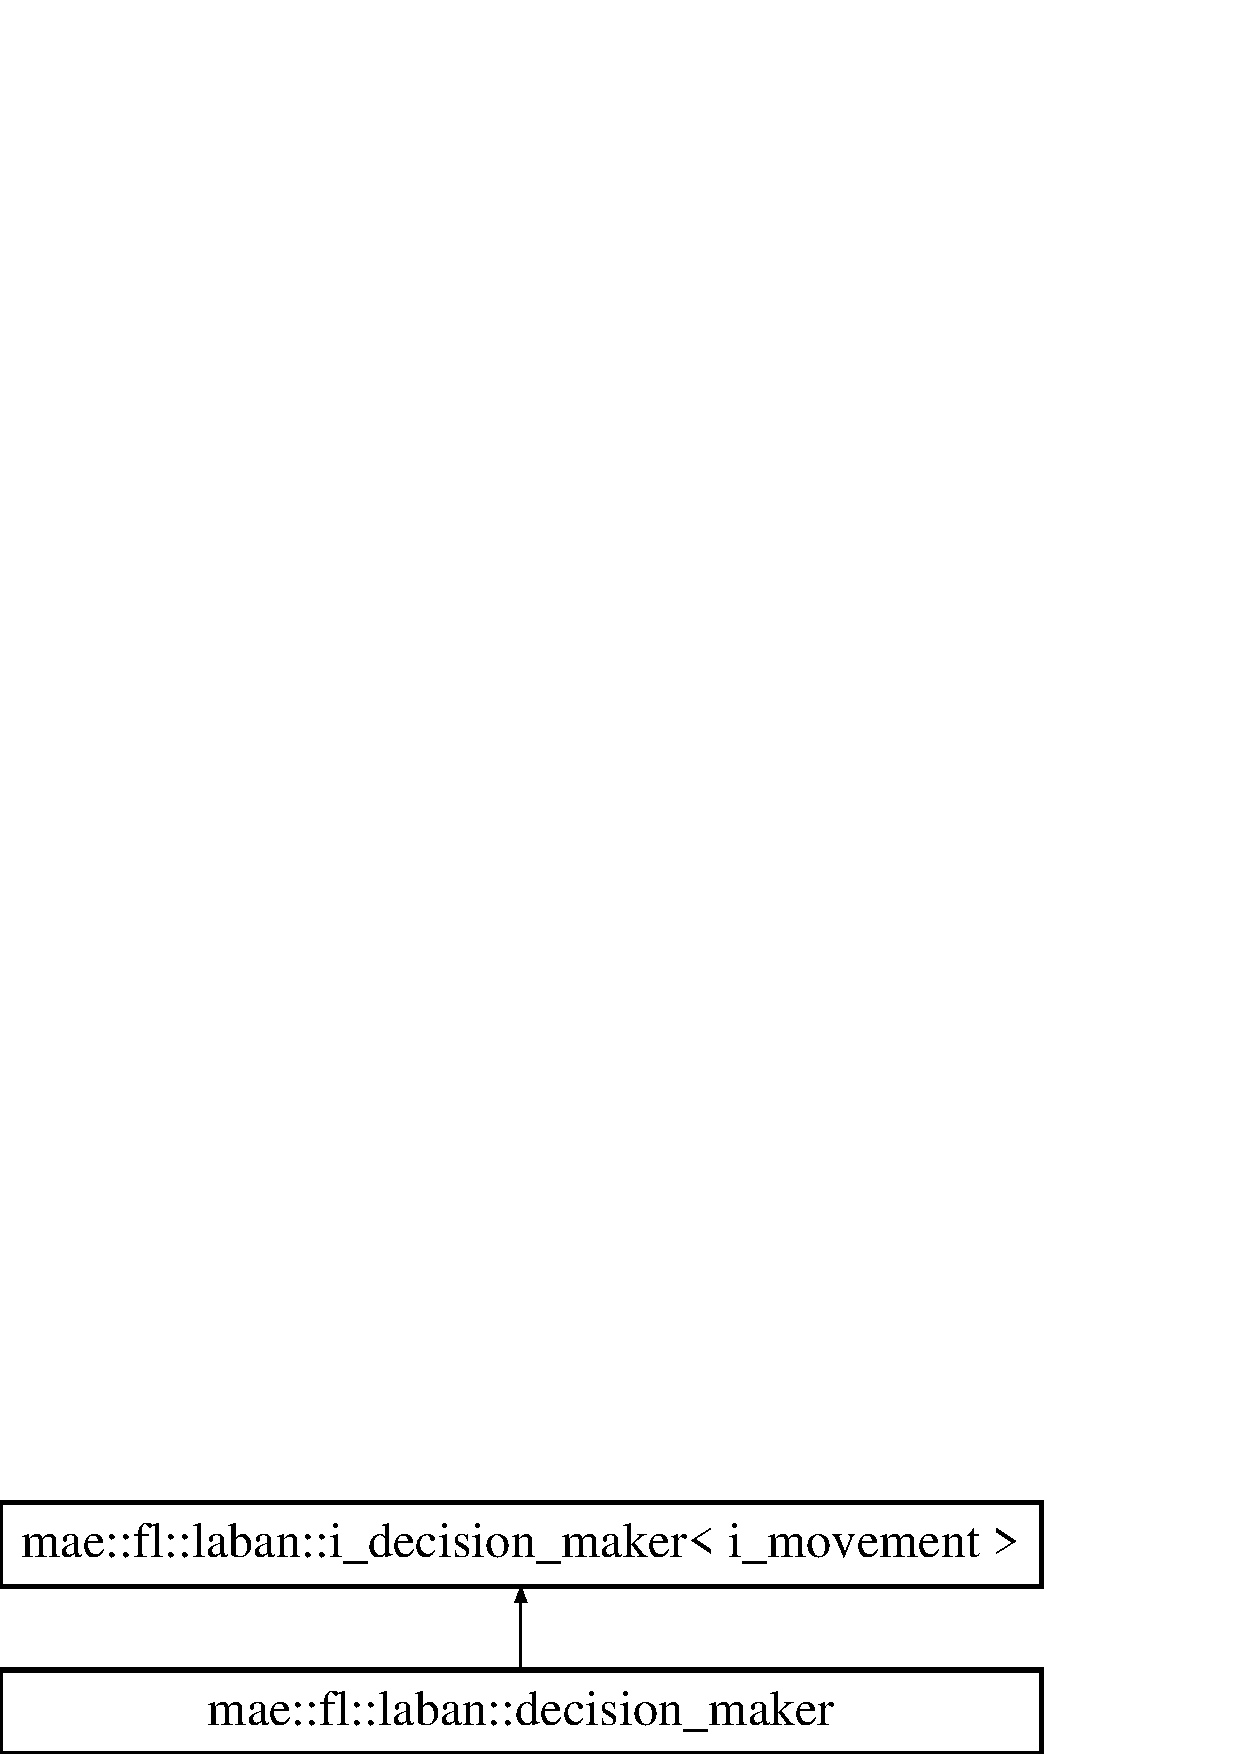
\includegraphics[height=2.000000cm]{classmae_1_1fl_1_1laban_1_1decision__maker}
\end{center}
\end{figure}
\subsection*{Public Member Functions}
\begin{DoxyCompactItemize}
\item 
\hyperlink{classmae_1_1fl_1_1laban_1_1decision__maker_abf4796f881cd73c9b4406bb1b6c7a84f}{decision\-\_\-maker} (int beats\-\_\-per\-\_\-measure, double tolerance=0.\-5, double start\-\_\-pose\-\_\-tolerance=0.\-5)
\item 
virtual void \hyperlink{classmae_1_1fl_1_1laban_1_1decision__maker_a7c83acb4810148453cee9f3098e89879}{set\-\_\-recognition\-\_\-tolerance} (double tolerance)
\item 
virtual double \hyperlink{classmae_1_1fl_1_1laban_1_1decision__maker_a3eb9245e5d7d34325051b91e8f20bd1b}{get\-\_\-recognition\-\_\-tolerance} ()
\item 
virtual void \hyperlink{classmae_1_1fl_1_1laban_1_1decision__maker_a93ac324bd228323cf0f1650dcd5f9f12}{set\-\_\-start\-\_\-pose\-\_\-tolerance} (double start\-\_\-pose\-\_\-tolerance)
\item 
virtual double \hyperlink{classmae_1_1fl_1_1laban_1_1decision__maker_ab3fadcd91ac85e52e8abeb8bdfe42bb4}{get\-\_\-start\-\_\-pose\-\_\-tolerance} ()
\item 
virtual bool \hyperlink{classmae_1_1fl_1_1laban_1_1decision__maker_aa620f89ab52dcfe3ceb7660898ae3988}{decide\-\_\-match} (std\-::shared\-\_\-ptr$<$ \hyperlink{classmae_1_1fl_1_1laban_1_1i__movement}{i\-\_\-movement} $>$ stream\-\_\-item, std\-::shared\-\_\-ptr$<$ \hyperlink{classmae_1_1fl_1_1laban_1_1i__movement}{i\-\_\-movement} $>$ stream\-\_\-item\-\_\-predecessor, std\-::shared\-\_\-ptr$<$ \hyperlink{classmae_1_1fl_1_1laban_1_1i__movement}{i\-\_\-movement} $>$ tree\-\_\-item, std\-::shared\-\_\-ptr$<$ \hyperlink{classmae_1_1fl_1_1laban_1_1i__movement}{i\-\_\-movement} $>$ tree\-\_\-item\-\_\-predecessor)
\item 
virtual bool \hyperlink{classmae_1_1fl_1_1laban_1_1decision__maker_ac1de2d370abf3d5ead61179eb5c318cc}{decide\-\_\-insertion} (std\-::shared\-\_\-ptr$<$ \hyperlink{classmae_1_1fl_1_1laban_1_1i__movement}{i\-\_\-movement} $>$ add\-\_\-item, std\-::shared\-\_\-ptr$<$ \hyperlink{classmae_1_1fl_1_1laban_1_1i__movement}{i\-\_\-movement} $>$ add\-\_\-item\-\_\-predecessor, std\-::shared\-\_\-ptr$<$ \hyperlink{classmae_1_1fl_1_1laban_1_1i__movement}{i\-\_\-movement} $>$ tree\-\_\-item, std\-::shared\-\_\-ptr$<$ \hyperlink{classmae_1_1fl_1_1laban_1_1i__movement}{i\-\_\-movement} $>$ tree\-\_\-item\-\_\-predecessor)
\item 
virtual bool \hyperlink{classmae_1_1fl_1_1laban_1_1decision__maker_af984822076ba7ef66bc54e1983366539}{position\-\_\-okay} (double dist\-\_\-to\-\_\-last, double set\-\_\-value, bool check\-\_\-startpose)
\end{DoxyCompactItemize}
\subsection*{Protected Member Functions}
\begin{DoxyCompactItemize}
\item 
virtual bool \hyperlink{classmae_1_1fl_1_1laban_1_1decision__maker_a4ce386b5214e83ef5abe2292f4e72949}{check\-\_\-position\-\_\-duration} (std\-::shared\-\_\-ptr$<$ \hyperlink{classmae_1_1fl_1_1laban_1_1i__movement}{i\-\_\-movement} $>$ stream\-\_\-item, std\-::shared\-\_\-ptr$<$ \hyperlink{classmae_1_1fl_1_1laban_1_1i__movement}{i\-\_\-movement} $>$ stream\-\_\-item\-\_\-predecessor, std\-::shared\-\_\-ptr$<$ \hyperlink{classmae_1_1fl_1_1laban_1_1i__movement}{i\-\_\-movement} $>$ tree\-\_\-item, std\-::shared\-\_\-ptr$<$ \hyperlink{classmae_1_1fl_1_1laban_1_1i__movement}{i\-\_\-movement} $>$ tree\-\_\-item\-\_\-predecessor)
\item 
virtual bool \hyperlink{classmae_1_1fl_1_1laban_1_1decision__maker_a2441c2dd64911691c3c526ab052ba297}{distance\-\_\-okay} (std\-::shared\-\_\-ptr$<$ \hyperlink{classmae_1_1fl_1_1laban_1_1i__movement}{i\-\_\-movement} $>$ dist\-\_\-from, std\-::shared\-\_\-ptr$<$ \hyperlink{classmae_1_1fl_1_1laban_1_1i__movement}{i\-\_\-movement} $>$ dist\-\_\-to, std\-::shared\-\_\-ptr$<$ \hyperlink{classmae_1_1fl_1_1laban_1_1i__movement}{i\-\_\-movement} $>$ check)
\item 
virtual bool \hyperlink{classmae_1_1fl_1_1laban_1_1decision__maker_af371be213337492cd49df8a7e0c24e8b}{check\-\_\-type} (std\-::shared\-\_\-ptr$<$ \hyperlink{classmae_1_1fl_1_1laban_1_1i__movement}{i\-\_\-movement} $>$ a, std\-::shared\-\_\-ptr$<$ \hyperlink{classmae_1_1fl_1_1laban_1_1i__movement}{i\-\_\-movement} $>$ b)
\end{DoxyCompactItemize}


\subsection{Constructor \& Destructor Documentation}
\hypertarget{classmae_1_1fl_1_1laban_1_1decision__maker_abf4796f881cd73c9b4406bb1b6c7a84f}{\index{mae\-::fl\-::laban\-::decision\-\_\-maker@{mae\-::fl\-::laban\-::decision\-\_\-maker}!decision\-\_\-maker@{decision\-\_\-maker}}
\index{decision\-\_\-maker@{decision\-\_\-maker}!mae::fl::laban::decision_maker@{mae\-::fl\-::laban\-::decision\-\_\-maker}}
\subsubsection[{decision\-\_\-maker}]{\setlength{\rightskip}{0pt plus 5cm}mae\-::fl\-::laban\-::decision\-\_\-maker\-::decision\-\_\-maker (
\begin{DoxyParamCaption}
\item[{int}]{beats\-\_\-per\-\_\-measure, }
\item[{double}]{tolerance = {\ttfamily 0.5}, }
\item[{double}]{start\-\_\-pose\-\_\-tolerance = {\ttfamily 0.5}}
\end{DoxyParamCaption}
)}}\label{classmae_1_1fl_1_1laban_1_1decision__maker_abf4796f881cd73c9b4406bb1b6c7a84f}
Creates a new decision maker.


\begin{DoxyParams}{Parameters}
{\em beats\-\_\-per\-\_\-measure} & The number of beats per measure for the present sequence of which movements are compared. \\
\hline
{\em tolerance} & The tolerance to be applied. It is given in beats and defines how many beats are accepted in deviance. \\
\hline
\end{DoxyParams}


\subsection{Member Function Documentation}
\hypertarget{classmae_1_1fl_1_1laban_1_1decision__maker_a4ce386b5214e83ef5abe2292f4e72949}{\index{mae\-::fl\-::laban\-::decision\-\_\-maker@{mae\-::fl\-::laban\-::decision\-\_\-maker}!check\-\_\-position\-\_\-duration@{check\-\_\-position\-\_\-duration}}
\index{check\-\_\-position\-\_\-duration@{check\-\_\-position\-\_\-duration}!mae::fl::laban::decision_maker@{mae\-::fl\-::laban\-::decision\-\_\-maker}}
\subsubsection[{check\-\_\-position\-\_\-duration}]{\setlength{\rightskip}{0pt plus 5cm}bool mae\-::fl\-::laban\-::decision\-\_\-maker\-::check\-\_\-position\-\_\-duration (
\begin{DoxyParamCaption}
\item[{std\-::shared\-\_\-ptr$<$ {\bf i\-\_\-movement} $>$}]{stream\-\_\-item, }
\item[{std\-::shared\-\_\-ptr$<$ {\bf i\-\_\-movement} $>$}]{stream\-\_\-item\-\_\-predecessor, }
\item[{std\-::shared\-\_\-ptr$<$ {\bf i\-\_\-movement} $>$}]{tree\-\_\-item, }
\item[{std\-::shared\-\_\-ptr$<$ {\bf i\-\_\-movement} $>$}]{tree\-\_\-item\-\_\-predecessor}
\end{DoxyParamCaption}
)\hspace{0.3cm}{\ttfamily [protected]}, {\ttfamily [virtual]}}}\label{classmae_1_1fl_1_1laban_1_1decision__maker_a4ce386b5214e83ef5abe2292f4e72949}
Checks whether position and duration match.


\begin{DoxyParams}{Parameters}
{\em stream\-\_\-item} & The element for the sequence to be matched. \\
\hline
{\em stream\-\_\-item\-\_\-predecessor} & The predecessor element for the sequence to be matched. \\
\hline
{\em tree\-\_\-item} & The decision tree's element. \\
\hline
{\em tree\-\_\-item\-\_\-predecessor} & The predecessor of the decision tree's element. \\
\hline
\end{DoxyParams}
\begin{DoxyReturn}{Returns}
True if positions and durations match. 
\end{DoxyReturn}
\hypertarget{classmae_1_1fl_1_1laban_1_1decision__maker_af371be213337492cd49df8a7e0c24e8b}{\index{mae\-::fl\-::laban\-::decision\-\_\-maker@{mae\-::fl\-::laban\-::decision\-\_\-maker}!check\-\_\-type@{check\-\_\-type}}
\index{check\-\_\-type@{check\-\_\-type}!mae::fl::laban::decision_maker@{mae\-::fl\-::laban\-::decision\-\_\-maker}}
\subsubsection[{check\-\_\-type}]{\setlength{\rightskip}{0pt plus 5cm}bool mae\-::fl\-::laban\-::decision\-\_\-maker\-::check\-\_\-type (
\begin{DoxyParamCaption}
\item[{std\-::shared\-\_\-ptr$<$ {\bf i\-\_\-movement} $>$}]{a, }
\item[{std\-::shared\-\_\-ptr$<$ {\bf i\-\_\-movement} $>$}]{b}
\end{DoxyParamCaption}
)\hspace{0.3cm}{\ttfamily [protected]}, {\ttfamily [virtual]}}}\label{classmae_1_1fl_1_1laban_1_1decision__maker_af371be213337492cd49df8a7e0c24e8b}
Checks whether the two movements are of the same type.


\begin{DoxyParams}{Parameters}
{\em a} & The first movement. \\
\hline
{\em b} & The second movement. \\
\hline
\end{DoxyParams}
\begin{DoxyReturn}{Returns}
True if matching. 
\end{DoxyReturn}
\hypertarget{classmae_1_1fl_1_1laban_1_1decision__maker_ac1de2d370abf3d5ead61179eb5c318cc}{\index{mae\-::fl\-::laban\-::decision\-\_\-maker@{mae\-::fl\-::laban\-::decision\-\_\-maker}!decide\-\_\-insertion@{decide\-\_\-insertion}}
\index{decide\-\_\-insertion@{decide\-\_\-insertion}!mae::fl::laban::decision_maker@{mae\-::fl\-::laban\-::decision\-\_\-maker}}
\subsubsection[{decide\-\_\-insertion}]{\setlength{\rightskip}{0pt plus 5cm}bool mae\-::fl\-::laban\-::decision\-\_\-maker\-::decide\-\_\-insertion (
\begin{DoxyParamCaption}
\item[{std\-::shared\-\_\-ptr$<$ {\bf i\-\_\-movement} $>$}]{add\-\_\-item, }
\item[{std\-::shared\-\_\-ptr$<$ {\bf i\-\_\-movement} $>$}]{add\-\_\-item\-\_\-predecessor, }
\item[{std\-::shared\-\_\-ptr$<$ {\bf i\-\_\-movement} $>$}]{tree\-\_\-item, }
\item[{std\-::shared\-\_\-ptr$<$ {\bf i\-\_\-movement} $>$}]{tree\-\_\-item\-\_\-predecessor}
\end{DoxyParamCaption}
)\hspace{0.3cm}{\ttfamily [virtual]}}}\label{classmae_1_1fl_1_1laban_1_1decision__maker_ac1de2d370abf3d5ead61179eb5c318cc}
Checks whether the two elements match in order to provide the decision result for an insertion. Their predecessors are provided in order to make more complex decisions.


\begin{DoxyParams}{Parameters}
{\em stream\-\_\-item} & The element for the sequence to be added. \\
\hline
{\em stream\-\_\-item\-\_\-predecessor} & The predecessor element for the sequence to be added. \\
\hline
{\em tree\-\_\-item} & The decision tree's element. \\
\hline
{\em tree\-\_\-item\-\_\-predecessor} & The predecessor of the decision tree's element. \\
\hline
\end{DoxyParams}
\begin{DoxyReturn}{Returns}

\end{DoxyReturn}


Implements \hyperlink{classmae_1_1fl_1_1laban_1_1i__decision__maker_a728e6e706f54a6f8dfbeff9a267afbf4}{mae\-::fl\-::laban\-::i\-\_\-decision\-\_\-maker$<$ i\-\_\-movement $>$}.

\hypertarget{classmae_1_1fl_1_1laban_1_1decision__maker_aa620f89ab52dcfe3ceb7660898ae3988}{\index{mae\-::fl\-::laban\-::decision\-\_\-maker@{mae\-::fl\-::laban\-::decision\-\_\-maker}!decide\-\_\-match@{decide\-\_\-match}}
\index{decide\-\_\-match@{decide\-\_\-match}!mae::fl::laban::decision_maker@{mae\-::fl\-::laban\-::decision\-\_\-maker}}
\subsubsection[{decide\-\_\-match}]{\setlength{\rightskip}{0pt plus 5cm}bool mae\-::fl\-::laban\-::decision\-\_\-maker\-::decide\-\_\-match (
\begin{DoxyParamCaption}
\item[{std\-::shared\-\_\-ptr$<$ {\bf i\-\_\-movement} $>$}]{stream\-\_\-item, }
\item[{std\-::shared\-\_\-ptr$<$ {\bf i\-\_\-movement} $>$}]{stream\-\_\-item\-\_\-predecessor, }
\item[{std\-::shared\-\_\-ptr$<$ {\bf i\-\_\-movement} $>$}]{tree\-\_\-item, }
\item[{std\-::shared\-\_\-ptr$<$ {\bf i\-\_\-movement} $>$}]{tree\-\_\-item\-\_\-predecessor}
\end{DoxyParamCaption}
)\hspace{0.3cm}{\ttfamily [virtual]}}}\label{classmae_1_1fl_1_1laban_1_1decision__maker_aa620f89ab52dcfe3ceb7660898ae3988}
Checks whether the two elements match in order to provide the decision result for a match. Their predecessors are provided in order to make more complex decisions.


\begin{DoxyParams}{Parameters}
{\em stream\-\_\-item} & The element for the sequence to be matched. \\
\hline
{\em stream\-\_\-item\-\_\-predecessor} & The predecessor element for the sequence to be matched. \\
\hline
{\em tree\-\_\-item} & The decision tree's element. \\
\hline
{\em tree\-\_\-item\-\_\-predecessor} & The predecessor of the decision tree's element. \\
\hline
\end{DoxyParams}
\begin{DoxyReturn}{Returns}
True if elements match. 
\end{DoxyReturn}


Implements \hyperlink{classmae_1_1fl_1_1laban_1_1i__decision__maker_ae1eb31ffcd38bcf0b207fee760ce98a6}{mae\-::fl\-::laban\-::i\-\_\-decision\-\_\-maker$<$ i\-\_\-movement $>$}.

\hypertarget{classmae_1_1fl_1_1laban_1_1decision__maker_a2441c2dd64911691c3c526ab052ba297}{\index{mae\-::fl\-::laban\-::decision\-\_\-maker@{mae\-::fl\-::laban\-::decision\-\_\-maker}!distance\-\_\-okay@{distance\-\_\-okay}}
\index{distance\-\_\-okay@{distance\-\_\-okay}!mae::fl::laban::decision_maker@{mae\-::fl\-::laban\-::decision\-\_\-maker}}
\subsubsection[{distance\-\_\-okay}]{\setlength{\rightskip}{0pt plus 5cm}bool mae\-::fl\-::laban\-::decision\-\_\-maker\-::distance\-\_\-okay (
\begin{DoxyParamCaption}
\item[{std\-::shared\-\_\-ptr$<$ {\bf i\-\_\-movement} $>$}]{dist\-\_\-from, }
\item[{std\-::shared\-\_\-ptr$<$ {\bf i\-\_\-movement} $>$}]{dist\-\_\-to, }
\item[{std\-::shared\-\_\-ptr$<$ {\bf i\-\_\-movement} $>$}]{check}
\end{DoxyParamCaption}
)\hspace{0.3cm}{\ttfamily [protected]}, {\ttfamily [virtual]}}}\label{classmae_1_1fl_1_1laban_1_1decision__maker_a2441c2dd64911691c3c526ab052ba297}
Checks the distance between the first to parameters and then examines whether the third parameter is matching. This is used to check whether the start pose does also match. Therefore distance between the two elements of the streamed sequence (potential first movement dist\-\_\-from and potential start pose dist\-\_\-to) are compared to the position of the first movement in the registered sequence (set value).


\begin{DoxyParams}{Parameters}
{\em dist\-\_\-from} & The distance from. \\
\hline
{\em dist\-\_\-to} & The distance to. \\
\hline
{\em check} & The element to be checked to have enough distance. \\
\hline
\end{DoxyParams}
\begin{DoxyReturn}{Returns}
True if distance is okay. 
\end{DoxyReturn}
\hypertarget{classmae_1_1fl_1_1laban_1_1decision__maker_a3eb9245e5d7d34325051b91e8f20bd1b}{\index{mae\-::fl\-::laban\-::decision\-\_\-maker@{mae\-::fl\-::laban\-::decision\-\_\-maker}!get\-\_\-recognition\-\_\-tolerance@{get\-\_\-recognition\-\_\-tolerance}}
\index{get\-\_\-recognition\-\_\-tolerance@{get\-\_\-recognition\-\_\-tolerance}!mae::fl::laban::decision_maker@{mae\-::fl\-::laban\-::decision\-\_\-maker}}
\subsubsection[{get\-\_\-recognition\-\_\-tolerance}]{\setlength{\rightskip}{0pt plus 5cm}double mae\-::fl\-::laban\-::decision\-\_\-maker\-::get\-\_\-recognition\-\_\-tolerance (
\begin{DoxyParamCaption}
{}
\end{DoxyParamCaption}
)\hspace{0.3cm}{\ttfamily [virtual]}}}\label{classmae_1_1fl_1_1laban_1_1decision__maker_a3eb9245e5d7d34325051b91e8f20bd1b}
Returns the tolerance for the recognition. The tolerance is a value which represents the number of beats of the labanotation which are tolerated in deviation.

\begin{DoxyReturn}{Returns}
The tolerance. 
\end{DoxyReturn}


Implements \hyperlink{classmae_1_1fl_1_1laban_1_1i__decision__maker_aa892f42c6407b3f8c9a67b71993103ea}{mae\-::fl\-::laban\-::i\-\_\-decision\-\_\-maker$<$ i\-\_\-movement $>$}.

\hypertarget{classmae_1_1fl_1_1laban_1_1decision__maker_ab3fadcd91ac85e52e8abeb8bdfe42bb4}{\index{mae\-::fl\-::laban\-::decision\-\_\-maker@{mae\-::fl\-::laban\-::decision\-\_\-maker}!get\-\_\-start\-\_\-pose\-\_\-tolerance@{get\-\_\-start\-\_\-pose\-\_\-tolerance}}
\index{get\-\_\-start\-\_\-pose\-\_\-tolerance@{get\-\_\-start\-\_\-pose\-\_\-tolerance}!mae::fl::laban::decision_maker@{mae\-::fl\-::laban\-::decision\-\_\-maker}}
\subsubsection[{get\-\_\-start\-\_\-pose\-\_\-tolerance}]{\setlength{\rightskip}{0pt plus 5cm}double mae\-::fl\-::laban\-::decision\-\_\-maker\-::get\-\_\-start\-\_\-pose\-\_\-tolerance (
\begin{DoxyParamCaption}
{}
\end{DoxyParamCaption}
)\hspace{0.3cm}{\ttfamily [virtual]}}}\label{classmae_1_1fl_1_1laban_1_1decision__maker_ab3fadcd91ac85e52e8abeb8bdfe42bb4}
Returns the tolerance for the recognition for one sided start poses (set value is start pose but actual movement is not).

\begin{DoxyReturn}{Returns}
The tolerance to be accepted. 
\end{DoxyReturn}
\hypertarget{classmae_1_1fl_1_1laban_1_1decision__maker_af984822076ba7ef66bc54e1983366539}{\index{mae\-::fl\-::laban\-::decision\-\_\-maker@{mae\-::fl\-::laban\-::decision\-\_\-maker}!position\-\_\-okay@{position\-\_\-okay}}
\index{position\-\_\-okay@{position\-\_\-okay}!mae::fl::laban::decision_maker@{mae\-::fl\-::laban\-::decision\-\_\-maker}}
\subsubsection[{position\-\_\-okay}]{\setlength{\rightskip}{0pt plus 5cm}bool mae\-::fl\-::laban\-::decision\-\_\-maker\-::position\-\_\-okay (
\begin{DoxyParamCaption}
\item[{double}]{dist\-\_\-to\-\_\-last, }
\item[{double}]{set\-\_\-value, }
\item[{bool}]{check\-\_\-startpose}
\end{DoxyParamCaption}
)\hspace{0.3cm}{\ttfamily [virtual]}}}\label{classmae_1_1fl_1_1laban_1_1decision__maker_af984822076ba7ef66bc54e1983366539}
Checks the distances of the last element in this column to the last element of all columns. The method takes care of start poses on the set value side, so that only minimum distance must match and not an interval.


\begin{DoxyParams}{Parameters}
{\em dist\-\_\-to\-\_\-last} & The distance to the last element of all columns. \\
\hline
{\em set\-\_\-value} & The set value for the distance. \\
\hline
{\em check\-\_\-startpose} & True if set value is to start pose but dist is not. \\
\hline
\end{DoxyParams}
\begin{DoxyReturn}{Returns}
True if accepted. 
\end{DoxyReturn}


Implements \hyperlink{classmae_1_1fl_1_1laban_1_1i__decision__maker_aad9230ee447afc0d6cf70cd74c54cf41}{mae\-::fl\-::laban\-::i\-\_\-decision\-\_\-maker$<$ i\-\_\-movement $>$}.

\hypertarget{classmae_1_1fl_1_1laban_1_1decision__maker_a7c83acb4810148453cee9f3098e89879}{\index{mae\-::fl\-::laban\-::decision\-\_\-maker@{mae\-::fl\-::laban\-::decision\-\_\-maker}!set\-\_\-recognition\-\_\-tolerance@{set\-\_\-recognition\-\_\-tolerance}}
\index{set\-\_\-recognition\-\_\-tolerance@{set\-\_\-recognition\-\_\-tolerance}!mae::fl::laban::decision_maker@{mae\-::fl\-::laban\-::decision\-\_\-maker}}
\subsubsection[{set\-\_\-recognition\-\_\-tolerance}]{\setlength{\rightskip}{0pt plus 5cm}void mae\-::fl\-::laban\-::decision\-\_\-maker\-::set\-\_\-recognition\-\_\-tolerance (
\begin{DoxyParamCaption}
\item[{double}]{tolerance}
\end{DoxyParamCaption}
)\hspace{0.3cm}{\ttfamily [virtual]}}}\label{classmae_1_1fl_1_1laban_1_1decision__maker_a7c83acb4810148453cee9f3098e89879}
Sets the tolerance for the recognition. The tolerance is a value which represents the number of beats of the labanotation which are tolerated in deviation.


\begin{DoxyParams}{Parameters}
{\em tolerance} & The tolerance to be accepted. \\
\hline
\end{DoxyParams}


Implements \hyperlink{classmae_1_1fl_1_1laban_1_1i__decision__maker_a63f05f6a3fb2a5f3b53f6555eada6243}{mae\-::fl\-::laban\-::i\-\_\-decision\-\_\-maker$<$ i\-\_\-movement $>$}.

\hypertarget{classmae_1_1fl_1_1laban_1_1decision__maker_a93ac324bd228323cf0f1650dcd5f9f12}{\index{mae\-::fl\-::laban\-::decision\-\_\-maker@{mae\-::fl\-::laban\-::decision\-\_\-maker}!set\-\_\-start\-\_\-pose\-\_\-tolerance@{set\-\_\-start\-\_\-pose\-\_\-tolerance}}
\index{set\-\_\-start\-\_\-pose\-\_\-tolerance@{set\-\_\-start\-\_\-pose\-\_\-tolerance}!mae::fl::laban::decision_maker@{mae\-::fl\-::laban\-::decision\-\_\-maker}}
\subsubsection[{set\-\_\-start\-\_\-pose\-\_\-tolerance}]{\setlength{\rightskip}{0pt plus 5cm}void mae\-::fl\-::laban\-::decision\-\_\-maker\-::set\-\_\-start\-\_\-pose\-\_\-tolerance (
\begin{DoxyParamCaption}
\item[{double}]{start\-\_\-pose\-\_\-tolerance}
\end{DoxyParamCaption}
)\hspace{0.3cm}{\ttfamily [virtual]}}}\label{classmae_1_1fl_1_1laban_1_1decision__maker_a93ac324bd228323cf0f1650dcd5f9f12}
Sets the tolerance for the recognition for one sided start poses (set value is start pose but actual movement is not).


\begin{DoxyParams}{Parameters}
{\em tolerance} & The tolerance to be accepted. \\
\hline
\end{DoxyParams}


The documentation for this class was generated from the following files\-:\begin{DoxyCompactItemize}
\item 
src/mae/fl/laban/decision\-\_\-maker.\-hpp\item 
src/mae/fl/laban/decision\-\_\-maker.\-cpp\end{DoxyCompactItemize}

\hypertarget{classmae_1_1fl_1_1laban_1_1decision__node}{\section{mae\-:\-:fl\-:\-:laban\-:\-:decision\-\_\-node$<$ T, U $>$ Class Template Reference}
\label{classmae_1_1fl_1_1laban_1_1decision__node}\index{mae\-::fl\-::laban\-::decision\-\_\-node$<$ T, U $>$@{mae\-::fl\-::laban\-::decision\-\_\-node$<$ T, U $>$}}
}
\subsection*{Public Member Functions}
\begin{DoxyCompactItemize}
\item 
\hyperlink{classmae_1_1fl_1_1laban_1_1decision__node_a3c90c6a24b41775eb5ce8fd259105db7}{decision\-\_\-node} (std\-::shared\-\_\-ptr$<$ \hyperlink{classmae_1_1fl_1_1laban_1_1i__decision__maker}{i\-\_\-decision\-\_\-maker}$<$ T $>$ $>$ \hyperlink{classmae_1_1fl_1_1laban_1_1decision__maker}{decision\-\_\-maker}, std\-::shared\-\_\-ptr$<$ T $>$ decision\-\_\-item)
\item 
virtual void \hyperlink{classmae_1_1fl_1_1laban_1_1decision__node_a90eeaa6db12b3c84ebf699f1a4e21e1a}{add\-\_\-sequence} (std\-::shared\-\_\-ptr$<$ \hyperlink{classmae_1_1fl_1_1laban_1_1decision__value}{decision\-\_\-value}$<$ T, U $>$ $>$ \hyperlink{classmae_1_1fl_1_1laban_1_1decision__value}{decision\-\_\-value}, int step, bool reverse\-\_\-order=false)
\item 
virtual bool \hyperlink{classmae_1_1fl_1_1laban_1_1decision__node_ab5aa2291848fd19563f7069ac9c67799}{remove\-\_\-where} (std\-::shared\-\_\-ptr$<$ U $>$ value)
\item 
virtual bool \hyperlink{classmae_1_1fl_1_1laban_1_1decision__node_a339862b47afb685f6d09fadd596bec60}{remove\-\_\-where} (std\-::shared\-\_\-ptr$<$ \hyperlink{classmae_1_1fl_1_1laban_1_1decision__value}{decision\-\_\-value}$<$ T, U $>$ $>$ dec\-\_\-val)
\item 
virtual std\-::vector\\*
$<$ std\-::shared\-\_\-ptr\\*
$<$ \hyperlink{classmae_1_1fl_1_1laban_1_1decision__value}{decision\-\_\-value}$<$ T, U $>$ $>$ $>$ \hyperlink{classmae_1_1fl_1_1laban_1_1decision__node_a2c770665666731e6cd69b157f696ab7b}{get\-\_\-all\-\_\-values} ()
\item 
virtual std\-::vector\\*
$<$ std\-::shared\-\_\-ptr\\*
$<$ \hyperlink{classmae_1_1fl_1_1laban_1_1decision__value}{decision\-\_\-value}$<$ T, U $>$ $>$ $>$ \hyperlink{classmae_1_1fl_1_1laban_1_1decision__node_a2e5f1b884ef53720015574306a5a35fd}{find\-\_\-submatches} (std\-::vector$<$ std\-::shared\-\_\-ptr$<$ T $>$ $>$ whole\-\_\-sequence, int step, int end\-\_\-pos=-\/1, bool reverse\-\_\-order=false)
\item 
virtual std\-::vector\\*
$<$ std\-::shared\-\_\-ptr\\*
$<$ \hyperlink{classmae_1_1fl_1_1laban_1_1decision__value}{decision\-\_\-value}$<$ T, U $>$ $>$ $>$ \hyperlink{classmae_1_1fl_1_1laban_1_1decision__node_a4191db14a5546c5343801be0b10a7f89}{find\-\_\-matches} (std\-::vector$<$ std\-::shared\-\_\-ptr$<$ T $>$ $>$ sequence, int step, int end\-\_\-pos=-\/1)
\item 
virtual std\-::vector\\*
$<$ std\-::shared\-\_\-ptr\\*
$<$ \hyperlink{classmae_1_1fl_1_1laban_1_1decision__node}{decision\-\_\-node}$<$ T, U $>$ $>$ $>$ \hyperlink{classmae_1_1fl_1_1laban_1_1decision__node_adf2c8d508c5b53d20b23694aa1f073f8}{get\-\_\-children} ()
\item 
virtual std\-::vector\\*
$<$ std\-::shared\-\_\-ptr\\*
$<$ \hyperlink{classmae_1_1fl_1_1laban_1_1decision__node}{decision\-\_\-node}$<$ T, U $>$ $>$ $>$ \hyperlink{classmae_1_1fl_1_1laban_1_1decision__node_ab070bdac746f755afdf23fe27a31fc56}{get\-\_\-matching\-\_\-children} (std\-::shared\-\_\-ptr$<$ T $>$ decision\-\_\-item, std\-::shared\-\_\-ptr$<$ T $>$ decision\-\_\-item\-\_\-predecessor, bool insertion=true)
\item 
virtual std\-::vector\\*
$<$ std\-::shared\-\_\-ptr\\*
$<$ \hyperlink{classmae_1_1fl_1_1laban_1_1decision__value}{decision\-\_\-value}$<$ T, U $>$ $>$ $>$ \hyperlink{classmae_1_1fl_1_1laban_1_1decision__node_ae7b51e4b1114f047d2c71da4faf1a4e3}{get\-\_\-node\-\_\-values} ()
\item 
virtual std\-::shared\-\_\-ptr$<$ T $>$ \hyperlink{classmae_1_1fl_1_1laban_1_1decision__node_a97f2e0467c0a4bd87e7d5e1cd3bf46fa}{get\-\_\-decision\-\_\-item} ()
\item 
virtual bool \hyperlink{classmae_1_1fl_1_1laban_1_1decision__node_a20907ce96f941914870cb5c7163584f7}{is\-\_\-matching} (std\-::shared\-\_\-ptr$<$ T $>$ decision\-\_\-item, std\-::shared\-\_\-ptr$<$ T $>$ decision\-\_\-item\-\_\-predecessor, std\-::shared\-\_\-ptr$<$ T $>$ decision\-\_\-item\-\_\-parent, bool insertion=true)
\item 
virtual bool \hyperlink{classmae_1_1fl_1_1laban_1_1decision__node_aece2f8658b9343c0bf6f80f090e01fa1}{is\-\_\-leaf} ()
\item 
virtual bool \hyperlink{classmae_1_1fl_1_1laban_1_1decision__node_a0494692662dd5b545b9c5db0b8fa7087}{is\-\_\-empty\-\_\-leaf} ()
\item 
virtual std\-::string \hyperlink{classmae_1_1fl_1_1laban_1_1decision__node_a1fd4ff5b5b5d5b0dac4502626e31b1fd}{str} (int indent=0)
\end{DoxyCompactItemize}


\subsection{Constructor \& Destructor Documentation}
\hypertarget{classmae_1_1fl_1_1laban_1_1decision__node_a3c90c6a24b41775eb5ce8fd259105db7}{\index{mae\-::fl\-::laban\-::decision\-\_\-node@{mae\-::fl\-::laban\-::decision\-\_\-node}!decision\-\_\-node@{decision\-\_\-node}}
\index{decision\-\_\-node@{decision\-\_\-node}!mae::fl::laban::decision_node@{mae\-::fl\-::laban\-::decision\-\_\-node}}
\subsubsection[{decision\-\_\-node}]{\setlength{\rightskip}{0pt plus 5cm}template$<$typename T , typename U $>$ {\bf mae\-::fl\-::laban\-::decision\-\_\-node}$<$ T, U $>$\-::{\bf decision\-\_\-node} (
\begin{DoxyParamCaption}
\item[{std\-::shared\-\_\-ptr$<$ {\bf i\-\_\-decision\-\_\-maker}$<$ T $>$ $>$}]{decision\-\_\-maker, }
\item[{std\-::shared\-\_\-ptr$<$ T $>$}]{decision\-\_\-item}
\end{DoxyParamCaption}
)}}\label{classmae_1_1fl_1_1laban_1_1decision__node_a3c90c6a24b41775eb5ce8fd259105db7}
Creates a decision node which is a node of the decision tree for sequences.


\begin{DoxyParams}{Parameters}
{\em \hyperlink{classmae_1_1fl_1_1laban_1_1decision__maker}{decision\-\_\-maker}} & The decision maker which is used to decide whether sequence elements are equal. \\
\hline
{\em decision\-\_\-item} & The item which is used to decide which sequence part this node matches. \\
\hline
\end{DoxyParams}


\subsection{Member Function Documentation}
\hypertarget{classmae_1_1fl_1_1laban_1_1decision__node_a90eeaa6db12b3c84ebf699f1a4e21e1a}{\index{mae\-::fl\-::laban\-::decision\-\_\-node@{mae\-::fl\-::laban\-::decision\-\_\-node}!add\-\_\-sequence@{add\-\_\-sequence}}
\index{add\-\_\-sequence@{add\-\_\-sequence}!mae::fl::laban::decision_node@{mae\-::fl\-::laban\-::decision\-\_\-node}}
\subsubsection[{add\-\_\-sequence}]{\setlength{\rightskip}{0pt plus 5cm}template$<$typename T , typename U $>$ void {\bf mae\-::fl\-::laban\-::decision\-\_\-node}$<$ T, U $>$\-::add\-\_\-sequence (
\begin{DoxyParamCaption}
\item[{std\-::shared\-\_\-ptr$<$ {\bf decision\-\_\-value}$<$ T, U $>$ $>$}]{decision\-\_\-value, }
\item[{int}]{step, }
\item[{bool}]{reverse\-\_\-order = {\ttfamily false}}
\end{DoxyParamCaption}
)\hspace{0.3cm}{\ttfamily [virtual]}}}\label{classmae_1_1fl_1_1laban_1_1decision__node_a90eeaa6db12b3c84ebf699f1a4e21e1a}
Adds a sequence to the node. Processes the children recursively. Adds children if decision elements are missing.


\begin{DoxyParams}{Parameters}
{\em sequence} & The sequence to be registered. Regards only the given body part. \\
\hline
{\em step} & The step which is used to identify a specific sequence element. \\
\hline
\end{DoxyParams}
\hypertarget{classmae_1_1fl_1_1laban_1_1decision__node_a4191db14a5546c5343801be0b10a7f89}{\index{mae\-::fl\-::laban\-::decision\-\_\-node@{mae\-::fl\-::laban\-::decision\-\_\-node}!find\-\_\-matches@{find\-\_\-matches}}
\index{find\-\_\-matches@{find\-\_\-matches}!mae::fl::laban::decision_node@{mae\-::fl\-::laban\-::decision\-\_\-node}}
\subsubsection[{find\-\_\-matches}]{\setlength{\rightskip}{0pt plus 5cm}template$<$typename T , typename U $>$ std\-::vector$<$ std\-::shared\-\_\-ptr$<$ {\bf decision\-\_\-value}$<$ T, U $>$ $>$ $>$ {\bf mae\-::fl\-::laban\-::decision\-\_\-node}$<$ T, U $>$\-::find\-\_\-matches (
\begin{DoxyParamCaption}
\item[{std\-::vector$<$ std\-::shared\-\_\-ptr$<$ T $>$ $>$}]{sequence, }
\item[{int}]{step, }
\item[{int}]{end\-\_\-pos = {\ttfamily -\/1}}
\end{DoxyParamCaption}
)\hspace{0.3cm}{\ttfamily [virtual]}}}\label{classmae_1_1fl_1_1laban_1_1decision__node_a4191db14a5546c5343801be0b10a7f89}
Finds exact matches starting at the step index. The order of the sequence must be of the same order as the added sequences.


\begin{DoxyParams}{Parameters}
{\em sequence} & The sequence to be matched. \\
\hline
{\em step} & The step index defining the start position for the match in this node. \\
\hline
{\em end\-\_\-pos} & The last position to be matched. -\/1 for last element of whole sequence. \\
\hline
\end{DoxyParams}
\begin{DoxyReturn}{Returns}
The matches. 
\end{DoxyReturn}
\hypertarget{classmae_1_1fl_1_1laban_1_1decision__node_a2e5f1b884ef53720015574306a5a35fd}{\index{mae\-::fl\-::laban\-::decision\-\_\-node@{mae\-::fl\-::laban\-::decision\-\_\-node}!find\-\_\-submatches@{find\-\_\-submatches}}
\index{find\-\_\-submatches@{find\-\_\-submatches}!mae::fl::laban::decision_node@{mae\-::fl\-::laban\-::decision\-\_\-node}}
\subsubsection[{find\-\_\-submatches}]{\setlength{\rightskip}{0pt plus 5cm}template$<$typename T , typename U $>$ std\-::vector$<$ std\-::shared\-\_\-ptr$<$ {\bf decision\-\_\-value}$<$ T, U $>$ $>$ $>$ {\bf mae\-::fl\-::laban\-::decision\-\_\-node}$<$ T, U $>$\-::find\-\_\-submatches (
\begin{DoxyParamCaption}
\item[{std\-::vector$<$ std\-::shared\-\_\-ptr$<$ T $>$ $>$}]{whole\-\_\-sequence, }
\item[{int}]{step, }
\item[{int}]{end\-\_\-pos = {\ttfamily -\/1}, }
\item[{bool}]{reverse\-\_\-order = {\ttfamily false}}
\end{DoxyParamCaption}
)\hspace{0.3cm}{\ttfamily [virtual]}}}\label{classmae_1_1fl_1_1laban_1_1decision__node_a2e5f1b884ef53720015574306a5a35fd}
Finds matches of subsequences in the whole sequence. This means that the whole sequences is looked up for having some of the registered sequences in it.


\begin{DoxyParams}{Parameters}
{\em whole\-\_\-sequence} & The whole sequence to be identified. \\
\hline
{\em step} & The step which is used to identify a specific sequence element. \\
\hline
{\em end\-\_\-pos} & The last step to be matched (no matter what the search order is, this values must be greater or equal the step value). -\/1 for last element of whole sequence. \\
\hline
{\em reverse\-\_\-order} & The order in which the submatches are searched. \\
\hline
\end{DoxyParams}
\begin{DoxyReturn}{Returns}
The submatches. 
\end{DoxyReturn}
\hypertarget{classmae_1_1fl_1_1laban_1_1decision__node_a2c770665666731e6cd69b157f696ab7b}{\index{mae\-::fl\-::laban\-::decision\-\_\-node@{mae\-::fl\-::laban\-::decision\-\_\-node}!get\-\_\-all\-\_\-values@{get\-\_\-all\-\_\-values}}
\index{get\-\_\-all\-\_\-values@{get\-\_\-all\-\_\-values}!mae::fl::laban::decision_node@{mae\-::fl\-::laban\-::decision\-\_\-node}}
\subsubsection[{get\-\_\-all\-\_\-values}]{\setlength{\rightskip}{0pt plus 5cm}template$<$typename T , typename U $>$ std\-::vector$<$ std\-::shared\-\_\-ptr$<$ {\bf decision\-\_\-value}$<$ T, U $>$ $>$ $>$ {\bf mae\-::fl\-::laban\-::decision\-\_\-node}$<$ T, U $>$\-::get\-\_\-all\-\_\-values (
\begin{DoxyParamCaption}
{}
\end{DoxyParamCaption}
)\hspace{0.3cm}{\ttfamily [virtual]}}}\label{classmae_1_1fl_1_1laban_1_1decision__node_a2c770665666731e6cd69b157f696ab7b}
Returns all registered values of the node and its children.

\begin{DoxyReturn}{Returns}
All values. 
\end{DoxyReturn}
\hypertarget{classmae_1_1fl_1_1laban_1_1decision__node_adf2c8d508c5b53d20b23694aa1f073f8}{\index{mae\-::fl\-::laban\-::decision\-\_\-node@{mae\-::fl\-::laban\-::decision\-\_\-node}!get\-\_\-children@{get\-\_\-children}}
\index{get\-\_\-children@{get\-\_\-children}!mae::fl::laban::decision_node@{mae\-::fl\-::laban\-::decision\-\_\-node}}
\subsubsection[{get\-\_\-children}]{\setlength{\rightskip}{0pt plus 5cm}template$<$typename T , typename U $>$ std\-::vector$<$ std\-::shared\-\_\-ptr$<$ {\bf decision\-\_\-node}$<$ T, U $>$ $>$ $>$ {\bf mae\-::fl\-::laban\-::decision\-\_\-node}$<$ T, U $>$\-::get\-\_\-children (
\begin{DoxyParamCaption}
{}
\end{DoxyParamCaption}
)\hspace{0.3cm}{\ttfamily [virtual]}}}\label{classmae_1_1fl_1_1laban_1_1decision__node_adf2c8d508c5b53d20b23694aa1f073f8}
Returns all children.

\begin{DoxyReturn}{Returns}
The children. 
\end{DoxyReturn}
\hypertarget{classmae_1_1fl_1_1laban_1_1decision__node_a97f2e0467c0a4bd87e7d5e1cd3bf46fa}{\index{mae\-::fl\-::laban\-::decision\-\_\-node@{mae\-::fl\-::laban\-::decision\-\_\-node}!get\-\_\-decision\-\_\-item@{get\-\_\-decision\-\_\-item}}
\index{get\-\_\-decision\-\_\-item@{get\-\_\-decision\-\_\-item}!mae::fl::laban::decision_node@{mae\-::fl\-::laban\-::decision\-\_\-node}}
\subsubsection[{get\-\_\-decision\-\_\-item}]{\setlength{\rightskip}{0pt plus 5cm}template$<$typename T , typename U $>$ std\-::shared\-\_\-ptr$<$ T $>$ {\bf mae\-::fl\-::laban\-::decision\-\_\-node}$<$ T, U $>$\-::get\-\_\-decision\-\_\-item (
\begin{DoxyParamCaption}
{}
\end{DoxyParamCaption}
)\hspace{0.3cm}{\ttfamily [virtual]}}}\label{classmae_1_1fl_1_1laban_1_1decision__node_a97f2e0467c0a4bd87e7d5e1cd3bf46fa}
Returns the item which is used to decide.

\begin{DoxyReturn}{Returns}
The decision item. 
\end{DoxyReturn}
\hypertarget{classmae_1_1fl_1_1laban_1_1decision__node_ab070bdac746f755afdf23fe27a31fc56}{\index{mae\-::fl\-::laban\-::decision\-\_\-node@{mae\-::fl\-::laban\-::decision\-\_\-node}!get\-\_\-matching\-\_\-children@{get\-\_\-matching\-\_\-children}}
\index{get\-\_\-matching\-\_\-children@{get\-\_\-matching\-\_\-children}!mae::fl::laban::decision_node@{mae\-::fl\-::laban\-::decision\-\_\-node}}
\subsubsection[{get\-\_\-matching\-\_\-children}]{\setlength{\rightskip}{0pt plus 5cm}template$<$typename T , typename U $>$ std\-::vector$<$ std\-::shared\-\_\-ptr$<$ {\bf decision\-\_\-node}$<$ T, U $>$ $>$ $>$ {\bf mae\-::fl\-::laban\-::decision\-\_\-node}$<$ T, U $>$\-::get\-\_\-matching\-\_\-children (
\begin{DoxyParamCaption}
\item[{std\-::shared\-\_\-ptr$<$ T $>$}]{decision\-\_\-item, }
\item[{std\-::shared\-\_\-ptr$<$ T $>$}]{decision\-\_\-item\-\_\-predecessor, }
\item[{bool}]{insertion = {\ttfamily true}}
\end{DoxyParamCaption}
)\hspace{0.3cm}{\ttfamily [virtual]}}}\label{classmae_1_1fl_1_1laban_1_1decision__node_ab070bdac746f755afdf23fe27a31fc56}
Returns all children that match the decision.


\begin{DoxyParams}{Parameters}
{\em decision\-\_\-item} & The item to be matched. \\
\hline
{\em insertion} & True if matching children for insertion. \\
\hline
\end{DoxyParams}
\begin{DoxyReturn}{Returns}
The child that matches the item. 
\end{DoxyReturn}
\hypertarget{classmae_1_1fl_1_1laban_1_1decision__node_ae7b51e4b1114f047d2c71da4faf1a4e3}{\index{mae\-::fl\-::laban\-::decision\-\_\-node@{mae\-::fl\-::laban\-::decision\-\_\-node}!get\-\_\-node\-\_\-values@{get\-\_\-node\-\_\-values}}
\index{get\-\_\-node\-\_\-values@{get\-\_\-node\-\_\-values}!mae::fl::laban::decision_node@{mae\-::fl\-::laban\-::decision\-\_\-node}}
\subsubsection[{get\-\_\-node\-\_\-values}]{\setlength{\rightskip}{0pt plus 5cm}template$<$typename T , typename U $>$ std\-::vector$<$ std\-::shared\-\_\-ptr$<$ {\bf decision\-\_\-value}$<$ T, U $>$ $>$ $>$ {\bf mae\-::fl\-::laban\-::decision\-\_\-node}$<$ T, U $>$\-::get\-\_\-node\-\_\-values (
\begin{DoxyParamCaption}
{}
\end{DoxyParamCaption}
)\hspace{0.3cm}{\ttfamily [virtual]}}}\label{classmae_1_1fl_1_1laban_1_1decision__node_ae7b51e4b1114f047d2c71da4faf1a4e3}
Returns the attached sequences which are those that begin with the assigned movement. \begin{DoxyReturn}{Returns}

\end{DoxyReturn}
\hypertarget{classmae_1_1fl_1_1laban_1_1decision__node_a0494692662dd5b545b9c5db0b8fa7087}{\index{mae\-::fl\-::laban\-::decision\-\_\-node@{mae\-::fl\-::laban\-::decision\-\_\-node}!is\-\_\-empty\-\_\-leaf@{is\-\_\-empty\-\_\-leaf}}
\index{is\-\_\-empty\-\_\-leaf@{is\-\_\-empty\-\_\-leaf}!mae::fl::laban::decision_node@{mae\-::fl\-::laban\-::decision\-\_\-node}}
\subsubsection[{is\-\_\-empty\-\_\-leaf}]{\setlength{\rightskip}{0pt plus 5cm}template$<$typename T , typename U $>$ bool {\bf mae\-::fl\-::laban\-::decision\-\_\-node}$<$ T, U $>$\-::is\-\_\-empty\-\_\-leaf (
\begin{DoxyParamCaption}
{}
\end{DoxyParamCaption}
)\hspace{0.3cm}{\ttfamily [virtual]}}}\label{classmae_1_1fl_1_1laban_1_1decision__node_a0494692662dd5b545b9c5db0b8fa7087}
Returns true if this node is a leaf and no values are attached.

\begin{DoxyReturn}{Returns}
True if empty leaf. 
\end{DoxyReturn}
\hypertarget{classmae_1_1fl_1_1laban_1_1decision__node_aece2f8658b9343c0bf6f80f090e01fa1}{\index{mae\-::fl\-::laban\-::decision\-\_\-node@{mae\-::fl\-::laban\-::decision\-\_\-node}!is\-\_\-leaf@{is\-\_\-leaf}}
\index{is\-\_\-leaf@{is\-\_\-leaf}!mae::fl::laban::decision_node@{mae\-::fl\-::laban\-::decision\-\_\-node}}
\subsubsection[{is\-\_\-leaf}]{\setlength{\rightskip}{0pt plus 5cm}template$<$typename T , typename U $>$ bool {\bf mae\-::fl\-::laban\-::decision\-\_\-node}$<$ T, U $>$\-::is\-\_\-leaf (
\begin{DoxyParamCaption}
{}
\end{DoxyParamCaption}
)\hspace{0.3cm}{\ttfamily [virtual]}}}\label{classmae_1_1fl_1_1laban_1_1decision__node_aece2f8658b9343c0bf6f80f090e01fa1}
Returns true if this node is a leaf.

\begin{DoxyReturn}{Returns}
True if leaf. 
\end{DoxyReturn}
\hypertarget{classmae_1_1fl_1_1laban_1_1decision__node_a20907ce96f941914870cb5c7163584f7}{\index{mae\-::fl\-::laban\-::decision\-\_\-node@{mae\-::fl\-::laban\-::decision\-\_\-node}!is\-\_\-matching@{is\-\_\-matching}}
\index{is\-\_\-matching@{is\-\_\-matching}!mae::fl::laban::decision_node@{mae\-::fl\-::laban\-::decision\-\_\-node}}
\subsubsection[{is\-\_\-matching}]{\setlength{\rightskip}{0pt plus 5cm}template$<$typename T , typename U $>$ bool {\bf mae\-::fl\-::laban\-::decision\-\_\-node}$<$ T, U $>$\-::is\-\_\-matching (
\begin{DoxyParamCaption}
\item[{std\-::shared\-\_\-ptr$<$ T $>$}]{decision\-\_\-item, }
\item[{std\-::shared\-\_\-ptr$<$ T $>$}]{decision\-\_\-item\-\_\-predecessor, }
\item[{std\-::shared\-\_\-ptr$<$ T $>$}]{decision\-\_\-item\-\_\-parent, }
\item[{bool}]{insertion = {\ttfamily true}}
\end{DoxyParamCaption}
)\hspace{0.3cm}{\ttfamily [virtual]}}}\label{classmae_1_1fl_1_1laban_1_1decision__node_a20907ce96f941914870cb5c7163584f7}
Returns true if this node's decision item is matching.


\begin{DoxyParams}{Parameters}
{\em decision\-\_\-item} & The other item (to be matched with). \\
\hline
{\em decision\-\_\-item\-\_\-predecessor} & The other item's predecessor. \\
\hline
{\em decision\-\_\-item\-\_\-parent} & This item's parent's item. \\
\hline
{\em insertion} & True if matching children for insertion. \\
\hline
\end{DoxyParams}
\begin{DoxyReturn}{Returns}
True if matching. 
\end{DoxyReturn}
\hypertarget{classmae_1_1fl_1_1laban_1_1decision__node_ab5aa2291848fd19563f7069ac9c67799}{\index{mae\-::fl\-::laban\-::decision\-\_\-node@{mae\-::fl\-::laban\-::decision\-\_\-node}!remove\-\_\-where@{remove\-\_\-where}}
\index{remove\-\_\-where@{remove\-\_\-where}!mae::fl::laban::decision_node@{mae\-::fl\-::laban\-::decision\-\_\-node}}
\subsubsection[{remove\-\_\-where}]{\setlength{\rightskip}{0pt plus 5cm}template$<$typename T , typename U $>$ bool {\bf mae\-::fl\-::laban\-::decision\-\_\-node}$<$ T, U $>$\-::remove\-\_\-where (
\begin{DoxyParamCaption}
\item[{std\-::shared\-\_\-ptr$<$ U $>$}]{value}
\end{DoxyParamCaption}
)\hspace{0.3cm}{\ttfamily [virtual]}}}\label{classmae_1_1fl_1_1laban_1_1decision__node_ab5aa2291848fd19563f7069ac9c67799}
Removes all decision values that have the given value.


\begin{DoxyParams}{Parameters}
{\em value} & The value used to decide removals. \\
\hline
\end{DoxyParams}
\begin{DoxyReturn}{Returns}
True if any removal was done. 
\end{DoxyReturn}
\hypertarget{classmae_1_1fl_1_1laban_1_1decision__node_a339862b47afb685f6d09fadd596bec60}{\index{mae\-::fl\-::laban\-::decision\-\_\-node@{mae\-::fl\-::laban\-::decision\-\_\-node}!remove\-\_\-where@{remove\-\_\-where}}
\index{remove\-\_\-where@{remove\-\_\-where}!mae::fl::laban::decision_node@{mae\-::fl\-::laban\-::decision\-\_\-node}}
\subsubsection[{remove\-\_\-where}]{\setlength{\rightskip}{0pt plus 5cm}template$<$typename T , typename U $>$ bool {\bf mae\-::fl\-::laban\-::decision\-\_\-node}$<$ T, U $>$\-::remove\-\_\-where (
\begin{DoxyParamCaption}
\item[{std\-::shared\-\_\-ptr$<$ {\bf decision\-\_\-value}$<$ T, U $>$ $>$}]{dec\-\_\-val}
\end{DoxyParamCaption}
)\hspace{0.3cm}{\ttfamily [virtual]}}}\label{classmae_1_1fl_1_1laban_1_1decision__node_a339862b47afb685f6d09fadd596bec60}
Removes the given decision value from all child nodes. Uses a smart pointer comparison for equality.


\begin{DoxyParams}{Parameters}
{\em dec\-\_\-val} & The decision value. \\
\hline
\end{DoxyParams}
\begin{DoxyReturn}{Returns}
True if any removal was done. 
\end{DoxyReturn}
\hypertarget{classmae_1_1fl_1_1laban_1_1decision__node_a1fd4ff5b5b5d5b0dac4502626e31b1fd}{\index{mae\-::fl\-::laban\-::decision\-\_\-node@{mae\-::fl\-::laban\-::decision\-\_\-node}!str@{str}}
\index{str@{str}!mae::fl::laban::decision_node@{mae\-::fl\-::laban\-::decision\-\_\-node}}
\subsubsection[{str}]{\setlength{\rightskip}{0pt plus 5cm}template$<$typename T , typename U $>$ std\-::string {\bf mae\-::fl\-::laban\-::decision\-\_\-node}$<$ T, U $>$\-::str (
\begin{DoxyParamCaption}
\item[{int}]{indent = {\ttfamily 0}}
\end{DoxyParamCaption}
)\hspace{0.3cm}{\ttfamily [virtual]}}}\label{classmae_1_1fl_1_1laban_1_1decision__node_a1fd4ff5b5b5d5b0dac4502626e31b1fd}
Returns the string representation for this node.


\begin{DoxyParams}{Parameters}
{\em indent} & The indent to be applied. \\
\hline
\end{DoxyParams}
\begin{DoxyReturn}{Returns}
The string. 
\end{DoxyReturn}


The documentation for this class was generated from the following file\-:\begin{DoxyCompactItemize}
\item 
src/mae/fl/laban/decision\-\_\-node.\-hpp\end{DoxyCompactItemize}

\hypertarget{classmae_1_1fl_1_1laban_1_1decision__tree}{\section{mae\-:\-:fl\-:\-:laban\-:\-:decision\-\_\-tree$<$ T, U $>$ Class Template Reference}
\label{classmae_1_1fl_1_1laban_1_1decision__tree}\index{mae\-::fl\-::laban\-::decision\-\_\-tree$<$ T, U $>$@{mae\-::fl\-::laban\-::decision\-\_\-tree$<$ T, U $>$}}
}
\subsection*{Public Member Functions}
\begin{DoxyCompactItemize}
\item 
\hyperlink{classmae_1_1fl_1_1laban_1_1decision__tree_ab918f661eaae6c18a4ac8700f13454c7}{decision\-\_\-tree} (std\-::shared\-\_\-ptr$<$ \hyperlink{classmae_1_1fl_1_1laban_1_1i__decision__maker}{i\-\_\-decision\-\_\-maker}$<$ T $>$ $>$ \hyperlink{classmae_1_1fl_1_1laban_1_1decision__maker}{decision\-\_\-maker})
\item 
virtual std\-::shared\-\_\-ptr\\*
$<$ \hyperlink{classmae_1_1fl_1_1laban_1_1decision__node}{decision\-\_\-node}$<$ T, U $>$ $>$ \hyperlink{classmae_1_1fl_1_1laban_1_1decision__tree_aaa7efdd0681f2497ab55c17955afbe53}{get\-\_\-root} ()
\item 
virtual bool \hyperlink{classmae_1_1fl_1_1laban_1_1decision__tree_ac41afc5b3c8000c5662893eee910d163}{is\-\_\-empty} ()
\item 
virtual void \hyperlink{classmae_1_1fl_1_1laban_1_1decision__tree_a6ddca3f455802ed8417473abeaab782b}{add\-\_\-sequence} (std\-::shared\-\_\-ptr$<$ \hyperlink{classmae_1_1fl_1_1laban_1_1decision__value}{decision\-\_\-value}$<$ T, U $>$ $>$ dec\-\_\-val, bool reverse\-\_\-order=false)
\item 
virtual std\-::vector\\*
$<$ std\-::shared\-\_\-ptr\\*
$<$ \hyperlink{classmae_1_1fl_1_1laban_1_1decision__value}{decision\-\_\-value}$<$ T, U $>$ $>$ $>$ \hyperlink{classmae_1_1fl_1_1laban_1_1decision__tree_a881223f0b283f7a6dc666fcf308b1db9}{get\-\_\-all\-\_\-values} ()
\item 
virtual bool \hyperlink{classmae_1_1fl_1_1laban_1_1decision__tree_a5131ee63acd1d486b5f6941eca413797}{remove\-\_\-where} (std\-::shared\-\_\-ptr$<$ U $>$ value)
\item 
virtual bool \hyperlink{classmae_1_1fl_1_1laban_1_1decision__tree_abe21b12fe75af8930074661bad98de70}{remove\-\_\-where} (std\-::shared\-\_\-ptr$<$ \hyperlink{classmae_1_1fl_1_1laban_1_1decision__value}{decision\-\_\-value}$<$ T, U $>$ $>$ dec\-\_\-val)
\item 
virtual std\-::vector\\*
$<$ std\-::shared\-\_\-ptr\\*
$<$ \hyperlink{classmae_1_1fl_1_1laban_1_1decision__value}{decision\-\_\-value}$<$ T, U $>$ $>$ $>$ \hyperlink{classmae_1_1fl_1_1laban_1_1decision__tree_aa8c955a5e5c1d372095b29be11ceb81f}{find\-\_\-submatches} (std\-::vector$<$ std\-::shared\-\_\-ptr$<$ T $>$ $>$ whole\-\_\-sequence, int start\-\_\-pos=0, int end\-\_\-pos=-\/1, bool reverse\-\_\-order=false)
\item 
virtual std\-::vector\\*
$<$ std\-::shared\-\_\-ptr\\*
$<$ \hyperlink{classmae_1_1fl_1_1laban_1_1decision__value}{decision\-\_\-value}$<$ T, U $>$ $>$ $>$ \hyperlink{classmae_1_1fl_1_1laban_1_1decision__tree_a6ab3d42b803e53fdc22879e42cae350a}{find\-\_\-matches} (std\-::vector$<$ std\-::shared\-\_\-ptr$<$ T $>$ $>$ sequence, int start\-\_\-pos=0, int end\-\_\-pos=-\/1)
\item 
virtual bool \hyperlink{classmae_1_1fl_1_1laban_1_1decision__tree_aca7c181ff309b41f333f40488beb7d09}{is\-\_\-root\-\_\-matching} (std\-::shared\-\_\-ptr$<$ T $>$ item) const 
\item 
virtual bool \hyperlink{classmae_1_1fl_1_1laban_1_1decision__tree_af60af0e00fd8e2ea821b0572ef8f1871}{is\-\_\-root\-\_\-insertion\-\_\-matching} (std\-::shared\-\_\-ptr$<$ T $>$ item) const 
\item 
virtual std\-::string \hyperlink{classmae_1_1fl_1_1laban_1_1decision__tree_a7eeabd5b8259cb334d30fd493bfb5f98}{str} ()
\end{DoxyCompactItemize}


\subsection{Constructor \& Destructor Documentation}
\hypertarget{classmae_1_1fl_1_1laban_1_1decision__tree_ab918f661eaae6c18a4ac8700f13454c7}{\index{mae\-::fl\-::laban\-::decision\-\_\-tree@{mae\-::fl\-::laban\-::decision\-\_\-tree}!decision\-\_\-tree@{decision\-\_\-tree}}
\index{decision\-\_\-tree@{decision\-\_\-tree}!mae::fl::laban::decision_tree@{mae\-::fl\-::laban\-::decision\-\_\-tree}}
\subsubsection[{decision\-\_\-tree}]{\setlength{\rightskip}{0pt plus 5cm}template$<$typename T , typename U $>$ {\bf mae\-::fl\-::laban\-::decision\-\_\-tree}$<$ T, U $>$\-::{\bf decision\-\_\-tree} (
\begin{DoxyParamCaption}
\item[{std\-::shared\-\_\-ptr$<$ {\bf i\-\_\-decision\-\_\-maker}$<$ T $>$ $>$}]{decision\-\_\-maker}
\end{DoxyParamCaption}
)}}\label{classmae_1_1fl_1_1laban_1_1decision__tree_ab918f661eaae6c18a4ac8700f13454c7}
Creates a new decision tree for sequences.


\begin{DoxyParams}{Parameters}
{\em body\-\_\-part} & The addressed body part. \\
\hline
{\em \hyperlink{classmae_1_1fl_1_1laban_1_1decision__maker}{decision\-\_\-maker}} & The decision maker which is used to decide whether two sequences are equal. \\
\hline
\end{DoxyParams}


\subsection{Member Function Documentation}
\hypertarget{classmae_1_1fl_1_1laban_1_1decision__tree_a6ddca3f455802ed8417473abeaab782b}{\index{mae\-::fl\-::laban\-::decision\-\_\-tree@{mae\-::fl\-::laban\-::decision\-\_\-tree}!add\-\_\-sequence@{add\-\_\-sequence}}
\index{add\-\_\-sequence@{add\-\_\-sequence}!mae::fl::laban::decision_tree@{mae\-::fl\-::laban\-::decision\-\_\-tree}}
\subsubsection[{add\-\_\-sequence}]{\setlength{\rightskip}{0pt plus 5cm}template$<$typename T , typename U $>$ void {\bf mae\-::fl\-::laban\-::decision\-\_\-tree}$<$ T, U $>$\-::add\-\_\-sequence (
\begin{DoxyParamCaption}
\item[{std\-::shared\-\_\-ptr$<$ {\bf decision\-\_\-value}$<$ T, U $>$ $>$}]{dec\-\_\-val, }
\item[{bool}]{reverse\-\_\-order = {\ttfamily false}}
\end{DoxyParamCaption}
)\hspace{0.3cm}{\ttfamily [virtual]}}}\label{classmae_1_1fl_1_1laban_1_1decision__tree_a6ddca3f455802ed8417473abeaab782b}
Adds a sequences to the tree. This may introduce new nodes to the tree.


\begin{DoxyParams}{Parameters}
{\em sequence} & The sequence to be registered. \\
\hline
{\em reverse\-\_\-order} & True if sequence shall be inserted in reverse order. \\
\hline
\end{DoxyParams}
\hypertarget{classmae_1_1fl_1_1laban_1_1decision__tree_a6ab3d42b803e53fdc22879e42cae350a}{\index{mae\-::fl\-::laban\-::decision\-\_\-tree@{mae\-::fl\-::laban\-::decision\-\_\-tree}!find\-\_\-matches@{find\-\_\-matches}}
\index{find\-\_\-matches@{find\-\_\-matches}!mae::fl::laban::decision_tree@{mae\-::fl\-::laban\-::decision\-\_\-tree}}
\subsubsection[{find\-\_\-matches}]{\setlength{\rightskip}{0pt plus 5cm}template$<$typename T , typename U $>$ std\-::vector$<$ std\-::shared\-\_\-ptr$<$ {\bf decision\-\_\-value}$<$ T, U $>$ $>$ $>$ {\bf mae\-::fl\-::laban\-::decision\-\_\-tree}$<$ T, U $>$\-::find\-\_\-matches (
\begin{DoxyParamCaption}
\item[{std\-::vector$<$ std\-::shared\-\_\-ptr$<$ T $>$ $>$}]{sequence, }
\item[{int}]{start\-\_\-pos = {\ttfamily 0}, }
\item[{int}]{end\-\_\-pos = {\ttfamily -\/1}}
\end{DoxyParamCaption}
)\hspace{0.3cm}{\ttfamily [virtual]}}}\label{classmae_1_1fl_1_1laban_1_1decision__tree_a6ab3d42b803e53fdc22879e42cae350a}
Finds exact matches of the given sequence starting at the given position. The order of the sequence must be of the same order as the added sequences.


\begin{DoxyParams}{Parameters}
{\em sequence} & The sequence. \\
\hline
{\em start\-\_\-pos} & The start position. \\
\hline
{\em end\-\_\-pos} & The last position to be matched. -\/1 for last element of whole sequence. \\
\hline
\end{DoxyParams}
\begin{DoxyReturn}{Returns}
All matches. 
\end{DoxyReturn}
\hypertarget{classmae_1_1fl_1_1laban_1_1decision__tree_aa8c955a5e5c1d372095b29be11ceb81f}{\index{mae\-::fl\-::laban\-::decision\-\_\-tree@{mae\-::fl\-::laban\-::decision\-\_\-tree}!find\-\_\-submatches@{find\-\_\-submatches}}
\index{find\-\_\-submatches@{find\-\_\-submatches}!mae::fl::laban::decision_tree@{mae\-::fl\-::laban\-::decision\-\_\-tree}}
\subsubsection[{find\-\_\-submatches}]{\setlength{\rightskip}{0pt plus 5cm}template$<$typename T , typename U $>$ std\-::vector$<$ std\-::shared\-\_\-ptr$<$ {\bf decision\-\_\-value}$<$ T, U $>$ $>$ $>$ {\bf mae\-::fl\-::laban\-::decision\-\_\-tree}$<$ T, U $>$\-::find\-\_\-submatches (
\begin{DoxyParamCaption}
\item[{std\-::vector$<$ std\-::shared\-\_\-ptr$<$ T $>$ $>$}]{whole\-\_\-sequence, }
\item[{int}]{start\-\_\-pos = {\ttfamily 0}, }
\item[{int}]{end\-\_\-pos = {\ttfamily -\/1}, }
\item[{bool}]{reverse\-\_\-order = {\ttfamily false}}
\end{DoxyParamCaption}
)\hspace{0.3cm}{\ttfamily [virtual]}}}\label{classmae_1_1fl_1_1laban_1_1decision__tree_aa8c955a5e5c1d372095b29be11ceb81f}
Searches the tree for all subsequences that match the decisions. The decision maker is checked for enough distance between a subsequence and the next element.


\begin{DoxyParams}{Parameters}
{\em whole\-\_\-sequence} & The whole sequence which is meant to be looked up for matches with the registered sequences. \\
\hline
{\em start\-\_\-pos} & The start position. \\
\hline
{\em end\-\_\-pos} & The last position to be matched. -\/1 for last element of whole sequence. \\
\hline
{\em reverse\-\_\-order} & The order in which the submatches are searched. \\
\hline
\end{DoxyParams}
\begin{DoxyReturn}{Returns}
All matches. 
\end{DoxyReturn}
\hypertarget{classmae_1_1fl_1_1laban_1_1decision__tree_a881223f0b283f7a6dc666fcf308b1db9}{\index{mae\-::fl\-::laban\-::decision\-\_\-tree@{mae\-::fl\-::laban\-::decision\-\_\-tree}!get\-\_\-all\-\_\-values@{get\-\_\-all\-\_\-values}}
\index{get\-\_\-all\-\_\-values@{get\-\_\-all\-\_\-values}!mae::fl::laban::decision_tree@{mae\-::fl\-::laban\-::decision\-\_\-tree}}
\subsubsection[{get\-\_\-all\-\_\-values}]{\setlength{\rightskip}{0pt plus 5cm}template$<$typename T , typename U $>$ std\-::vector$<$ std\-::shared\-\_\-ptr$<$ {\bf decision\-\_\-value}$<$ T, U $>$ $>$ $>$ {\bf mae\-::fl\-::laban\-::decision\-\_\-tree}$<$ T, U $>$\-::get\-\_\-all\-\_\-values (
\begin{DoxyParamCaption}
{}
\end{DoxyParamCaption}
)\hspace{0.3cm}{\ttfamily [virtual]}}}\label{classmae_1_1fl_1_1laban_1_1decision__tree_a881223f0b283f7a6dc666fcf308b1db9}
Returns all registered values of the tree.

\begin{DoxyReturn}{Returns}
The values. 
\end{DoxyReturn}
\hypertarget{classmae_1_1fl_1_1laban_1_1decision__tree_aaa7efdd0681f2497ab55c17955afbe53}{\index{mae\-::fl\-::laban\-::decision\-\_\-tree@{mae\-::fl\-::laban\-::decision\-\_\-tree}!get\-\_\-root@{get\-\_\-root}}
\index{get\-\_\-root@{get\-\_\-root}!mae::fl::laban::decision_tree@{mae\-::fl\-::laban\-::decision\-\_\-tree}}
\subsubsection[{get\-\_\-root}]{\setlength{\rightskip}{0pt plus 5cm}template$<$typename T , typename U $>$ std\-::shared\-\_\-ptr$<$ {\bf decision\-\_\-node}$<$ T, U $>$ $>$ {\bf mae\-::fl\-::laban\-::decision\-\_\-tree}$<$ T, U $>$\-::get\-\_\-root (
\begin{DoxyParamCaption}
{}
\end{DoxyParamCaption}
)\hspace{0.3cm}{\ttfamily [virtual]}}}\label{classmae_1_1fl_1_1laban_1_1decision__tree_aaa7efdd0681f2497ab55c17955afbe53}
Returns the root node if any. Returns null otherwise.

\begin{DoxyReturn}{Returns}
The root element. 
\end{DoxyReturn}
\hypertarget{classmae_1_1fl_1_1laban_1_1decision__tree_ac41afc5b3c8000c5662893eee910d163}{\index{mae\-::fl\-::laban\-::decision\-\_\-tree@{mae\-::fl\-::laban\-::decision\-\_\-tree}!is\-\_\-empty@{is\-\_\-empty}}
\index{is\-\_\-empty@{is\-\_\-empty}!mae::fl::laban::decision_tree@{mae\-::fl\-::laban\-::decision\-\_\-tree}}
\subsubsection[{is\-\_\-empty}]{\setlength{\rightskip}{0pt plus 5cm}template$<$typename T , typename U $>$ bool {\bf mae\-::fl\-::laban\-::decision\-\_\-tree}$<$ T, U $>$\-::is\-\_\-empty (
\begin{DoxyParamCaption}
{}
\end{DoxyParamCaption}
)\hspace{0.3cm}{\ttfamily [virtual]}}}\label{classmae_1_1fl_1_1laban_1_1decision__tree_ac41afc5b3c8000c5662893eee910d163}
Returns true if the sequence is empty (meaning the not root is assigned or the whole tree contains no elements).

\begin{DoxyReturn}{Returns}
True if empty. 
\end{DoxyReturn}
\hypertarget{classmae_1_1fl_1_1laban_1_1decision__tree_af60af0e00fd8e2ea821b0572ef8f1871}{\index{mae\-::fl\-::laban\-::decision\-\_\-tree@{mae\-::fl\-::laban\-::decision\-\_\-tree}!is\-\_\-root\-\_\-insertion\-\_\-matching@{is\-\_\-root\-\_\-insertion\-\_\-matching}}
\index{is\-\_\-root\-\_\-insertion\-\_\-matching@{is\-\_\-root\-\_\-insertion\-\_\-matching}!mae::fl::laban::decision_tree@{mae\-::fl\-::laban\-::decision\-\_\-tree}}
\subsubsection[{is\-\_\-root\-\_\-insertion\-\_\-matching}]{\setlength{\rightskip}{0pt plus 5cm}template$<$typename T , typename U $>$ bool {\bf mae\-::fl\-::laban\-::decision\-\_\-tree}$<$ T, U $>$\-::is\-\_\-root\-\_\-insertion\-\_\-matching (
\begin{DoxyParamCaption}
\item[{std\-::shared\-\_\-ptr$<$ T $>$}]{item}
\end{DoxyParamCaption}
) const\hspace{0.3cm}{\ttfamily [virtual]}}}\label{classmae_1_1fl_1_1laban_1_1decision__tree_af60af0e00fd8e2ea821b0572ef8f1871}
Returns true if the root element matches the given item for a insertion.


\begin{DoxyParams}{Parameters}
{\em item} & The item to be compared using the decision maker. \\
\hline
\end{DoxyParams}
\begin{DoxyReturn}{Returns}
True if matching. 
\end{DoxyReturn}
\hypertarget{classmae_1_1fl_1_1laban_1_1decision__tree_aca7c181ff309b41f333f40488beb7d09}{\index{mae\-::fl\-::laban\-::decision\-\_\-tree@{mae\-::fl\-::laban\-::decision\-\_\-tree}!is\-\_\-root\-\_\-matching@{is\-\_\-root\-\_\-matching}}
\index{is\-\_\-root\-\_\-matching@{is\-\_\-root\-\_\-matching}!mae::fl::laban::decision_tree@{mae\-::fl\-::laban\-::decision\-\_\-tree}}
\subsubsection[{is\-\_\-root\-\_\-matching}]{\setlength{\rightskip}{0pt plus 5cm}template$<$typename T , typename U $>$ bool {\bf mae\-::fl\-::laban\-::decision\-\_\-tree}$<$ T, U $>$\-::is\-\_\-root\-\_\-matching (
\begin{DoxyParamCaption}
\item[{std\-::shared\-\_\-ptr$<$ T $>$}]{item}
\end{DoxyParamCaption}
) const\hspace{0.3cm}{\ttfamily [virtual]}}}\label{classmae_1_1fl_1_1laban_1_1decision__tree_aca7c181ff309b41f333f40488beb7d09}
Returns true if the root element matches the given item.


\begin{DoxyParams}{Parameters}
{\em item} & The item to be compared using the decision maker. \\
\hline
\end{DoxyParams}
\begin{DoxyReturn}{Returns}
True if matching. 
\end{DoxyReturn}
\hypertarget{classmae_1_1fl_1_1laban_1_1decision__tree_a5131ee63acd1d486b5f6941eca413797}{\index{mae\-::fl\-::laban\-::decision\-\_\-tree@{mae\-::fl\-::laban\-::decision\-\_\-tree}!remove\-\_\-where@{remove\-\_\-where}}
\index{remove\-\_\-where@{remove\-\_\-where}!mae::fl::laban::decision_tree@{mae\-::fl\-::laban\-::decision\-\_\-tree}}
\subsubsection[{remove\-\_\-where}]{\setlength{\rightskip}{0pt plus 5cm}template$<$typename T , typename U $>$ bool {\bf mae\-::fl\-::laban\-::decision\-\_\-tree}$<$ T, U $>$\-::remove\-\_\-where (
\begin{DoxyParamCaption}
\item[{std\-::shared\-\_\-ptr$<$ U $>$}]{value}
\end{DoxyParamCaption}
)\hspace{0.3cm}{\ttfamily [virtual]}}}\label{classmae_1_1fl_1_1laban_1_1decision__tree_a5131ee63acd1d486b5f6941eca413797}
Removes all decision values where the value element is the given one. Equality is checked by the pointer.


\begin{DoxyParams}{Parameters}
{\em value} & The value. \\
\hline
\end{DoxyParams}
\begin{DoxyReturn}{Returns}
True if any removal was done. 
\end{DoxyReturn}
\hypertarget{classmae_1_1fl_1_1laban_1_1decision__tree_abe21b12fe75af8930074661bad98de70}{\index{mae\-::fl\-::laban\-::decision\-\_\-tree@{mae\-::fl\-::laban\-::decision\-\_\-tree}!remove\-\_\-where@{remove\-\_\-where}}
\index{remove\-\_\-where@{remove\-\_\-where}!mae::fl::laban::decision_tree@{mae\-::fl\-::laban\-::decision\-\_\-tree}}
\subsubsection[{remove\-\_\-where}]{\setlength{\rightskip}{0pt plus 5cm}template$<$typename T , typename U $>$ bool {\bf mae\-::fl\-::laban\-::decision\-\_\-tree}$<$ T, U $>$\-::remove\-\_\-where (
\begin{DoxyParamCaption}
\item[{std\-::shared\-\_\-ptr$<$ {\bf decision\-\_\-value}$<$ T, U $>$ $>$}]{dec\-\_\-val}
\end{DoxyParamCaption}
)\hspace{0.3cm}{\ttfamily [virtual]}}}\label{classmae_1_1fl_1_1laban_1_1decision__tree_abe21b12fe75af8930074661bad98de70}
Removes all entries for the decision value in the tree.


\begin{DoxyParams}{Parameters}
{\em dec\-\_\-val} & The decision item. \\
\hline
\end{DoxyParams}
\begin{DoxyReturn}{Returns}
True if any removal was done. 
\end{DoxyReturn}
\hypertarget{classmae_1_1fl_1_1laban_1_1decision__tree_a7eeabd5b8259cb334d30fd493bfb5f98}{\index{mae\-::fl\-::laban\-::decision\-\_\-tree@{mae\-::fl\-::laban\-::decision\-\_\-tree}!str@{str}}
\index{str@{str}!mae::fl::laban::decision_tree@{mae\-::fl\-::laban\-::decision\-\_\-tree}}
\subsubsection[{str}]{\setlength{\rightskip}{0pt plus 5cm}template$<$typename T , typename U $>$ std\-::string {\bf mae\-::fl\-::laban\-::decision\-\_\-tree}$<$ T, U $>$\-::str (
\begin{DoxyParamCaption}
{}
\end{DoxyParamCaption}
)\hspace{0.3cm}{\ttfamily [virtual]}}}\label{classmae_1_1fl_1_1laban_1_1decision__tree_a7eeabd5b8259cb334d30fd493bfb5f98}
Returns the string representation for this tree. \begin{DoxyReturn}{Returns}
The string. 
\end{DoxyReturn}


The documentation for this class was generated from the following file\-:\begin{DoxyCompactItemize}
\item 
src/mae/fl/laban/decision\-\_\-tree.\-hpp\end{DoxyCompactItemize}

\hypertarget{classmae_1_1fl_1_1laban_1_1decision__value}{\section{mae\-:\-:fl\-:\-:laban\-:\-:decision\-\_\-value$<$ T, U $>$ Class Template Reference}
\label{classmae_1_1fl_1_1laban_1_1decision__value}\index{mae\-::fl\-::laban\-::decision\-\_\-value$<$ T, U $>$@{mae\-::fl\-::laban\-::decision\-\_\-value$<$ T, U $>$}}
}
\subsection*{Public Member Functions}
\begin{DoxyCompactItemize}
\item 
\hyperlink{classmae_1_1fl_1_1laban_1_1decision__value_a44fec52cd646784da3b3ddb93f49082d}{decision\-\_\-value} (std\-::vector$<$ std\-::shared\-\_\-ptr$<$ T $>$ $>$ sequence, std\-::shared\-\_\-ptr$<$ U $>$ value)
\item 
\hyperlink{classmae_1_1fl_1_1laban_1_1decision__value_ae11cae0f22f4403843f88516185f9cb3}{decision\-\_\-value} (std\-::shared\-\_\-ptr$<$ U $>$ value)
\item 
virtual std\-::vector\\*
$<$ std\-::shared\-\_\-ptr$<$ T $>$ $>$ \hyperlink{classmae_1_1fl_1_1laban_1_1decision__value_a1b71fb8f5636784448b847488cf686d4}{get\-\_\-sequence} ()
\item 
virtual std\-::shared\-\_\-ptr$<$ U $>$ \hyperlink{classmae_1_1fl_1_1laban_1_1decision__value_ad0d4a61c756c56be2fb1a94b160d11b2}{get\-\_\-value} ()
\end{DoxyCompactItemize}


\subsection{Constructor \& Destructor Documentation}
\hypertarget{classmae_1_1fl_1_1laban_1_1decision__value_a44fec52cd646784da3b3ddb93f49082d}{\index{mae\-::fl\-::laban\-::decision\-\_\-value@{mae\-::fl\-::laban\-::decision\-\_\-value}!decision\-\_\-value@{decision\-\_\-value}}
\index{decision\-\_\-value@{decision\-\_\-value}!mae::fl::laban::decision_value@{mae\-::fl\-::laban\-::decision\-\_\-value}}
\subsubsection[{decision\-\_\-value}]{\setlength{\rightskip}{0pt plus 5cm}template$<$typename T , typename U $>$ {\bf mae\-::fl\-::laban\-::decision\-\_\-value}$<$ T, U $>$\-::{\bf decision\-\_\-value} (
\begin{DoxyParamCaption}
\item[{std\-::vector$<$ std\-::shared\-\_\-ptr$<$ T $>$ $>$}]{sequence, }
\item[{std\-::shared\-\_\-ptr$<$ U $>$}]{value}
\end{DoxyParamCaption}
)}}\label{classmae_1_1fl_1_1laban_1_1decision__value_a44fec52cd646784da3b3ddb93f49082d}
Creates a new decision value for a sequence. It contains the sequence and the associated value.


\begin{DoxyParams}{Parameters}
{\em sequence} & The sequence. \\
\hline
{\em value} & The value. \\
\hline
\end{DoxyParams}
\hypertarget{classmae_1_1fl_1_1laban_1_1decision__value_ae11cae0f22f4403843f88516185f9cb3}{\index{mae\-::fl\-::laban\-::decision\-\_\-value@{mae\-::fl\-::laban\-::decision\-\_\-value}!decision\-\_\-value@{decision\-\_\-value}}
\index{decision\-\_\-value@{decision\-\_\-value}!mae::fl::laban::decision_value@{mae\-::fl\-::laban\-::decision\-\_\-value}}
\subsubsection[{decision\-\_\-value}]{\setlength{\rightskip}{0pt plus 5cm}template$<$typename T , typename U $>$ {\bf mae\-::fl\-::laban\-::decision\-\_\-value}$<$ T, U $>$\-::{\bf decision\-\_\-value} (
\begin{DoxyParamCaption}
\item[{std\-::shared\-\_\-ptr$<$ U $>$}]{value}
\end{DoxyParamCaption}
)}}\label{classmae_1_1fl_1_1laban_1_1decision__value_ae11cae0f22f4403843f88516185f9cb3}
Creates a new decision value for a sequence. It contains the sequence, which in this case is assumed to be empty, and the associated value.


\begin{DoxyParams}{Parameters}
{\em value} & The value. \\
\hline
\end{DoxyParams}


\subsection{Member Function Documentation}
\hypertarget{classmae_1_1fl_1_1laban_1_1decision__value_a1b71fb8f5636784448b847488cf686d4}{\index{mae\-::fl\-::laban\-::decision\-\_\-value@{mae\-::fl\-::laban\-::decision\-\_\-value}!get\-\_\-sequence@{get\-\_\-sequence}}
\index{get\-\_\-sequence@{get\-\_\-sequence}!mae::fl::laban::decision_value@{mae\-::fl\-::laban\-::decision\-\_\-value}}
\subsubsection[{get\-\_\-sequence}]{\setlength{\rightskip}{0pt plus 5cm}template$<$typename T , typename U $>$ std\-::vector$<$ std\-::shared\-\_\-ptr$<$ T $>$ $>$ {\bf mae\-::fl\-::laban\-::decision\-\_\-value}$<$ T, U $>$\-::get\-\_\-sequence (
\begin{DoxyParamCaption}
{}
\end{DoxyParamCaption}
)\hspace{0.3cm}{\ttfamily [virtual]}}}\label{classmae_1_1fl_1_1laban_1_1decision__value_a1b71fb8f5636784448b847488cf686d4}
Returns the sequence.

\begin{DoxyReturn}{Returns}
The sequence. 
\end{DoxyReturn}
\hypertarget{classmae_1_1fl_1_1laban_1_1decision__value_ad0d4a61c756c56be2fb1a94b160d11b2}{\index{mae\-::fl\-::laban\-::decision\-\_\-value@{mae\-::fl\-::laban\-::decision\-\_\-value}!get\-\_\-value@{get\-\_\-value}}
\index{get\-\_\-value@{get\-\_\-value}!mae::fl::laban::decision_value@{mae\-::fl\-::laban\-::decision\-\_\-value}}
\subsubsection[{get\-\_\-value}]{\setlength{\rightskip}{0pt plus 5cm}template$<$typename T , typename U $>$ std\-::shared\-\_\-ptr$<$ U $>$ {\bf mae\-::fl\-::laban\-::decision\-\_\-value}$<$ T, U $>$\-::get\-\_\-value (
\begin{DoxyParamCaption}
{}
\end{DoxyParamCaption}
)\hspace{0.3cm}{\ttfamily [virtual]}}}\label{classmae_1_1fl_1_1laban_1_1decision__value_ad0d4a61c756c56be2fb1a94b160d11b2}
Returns the value.

\begin{DoxyReturn}{Returns}
The value. 
\end{DoxyReturn}


The documentation for this class was generated from the following file\-:\begin{DoxyCompactItemize}
\item 
src/mae/fl/laban/decision\-\_\-value.\-hpp\end{DoxyCompactItemize}

\hypertarget{classmae_1_1fl_1_1laban_1_1ps_1_1default__limb}{\section{mae\-:\-:fl\-:\-:laban\-:\-:ps\-:\-:default\-\_\-limb Class Reference}
\label{classmae_1_1fl_1_1laban_1_1ps_1_1default__limb}\index{mae\-::fl\-::laban\-::ps\-::default\-\_\-limb@{mae\-::fl\-::laban\-::ps\-::default\-\_\-limb}}
}
Inheritance diagram for mae\-:\-:fl\-:\-:laban\-:\-:ps\-:\-:default\-\_\-limb\-:\begin{figure}[H]
\begin{center}
\leavevmode
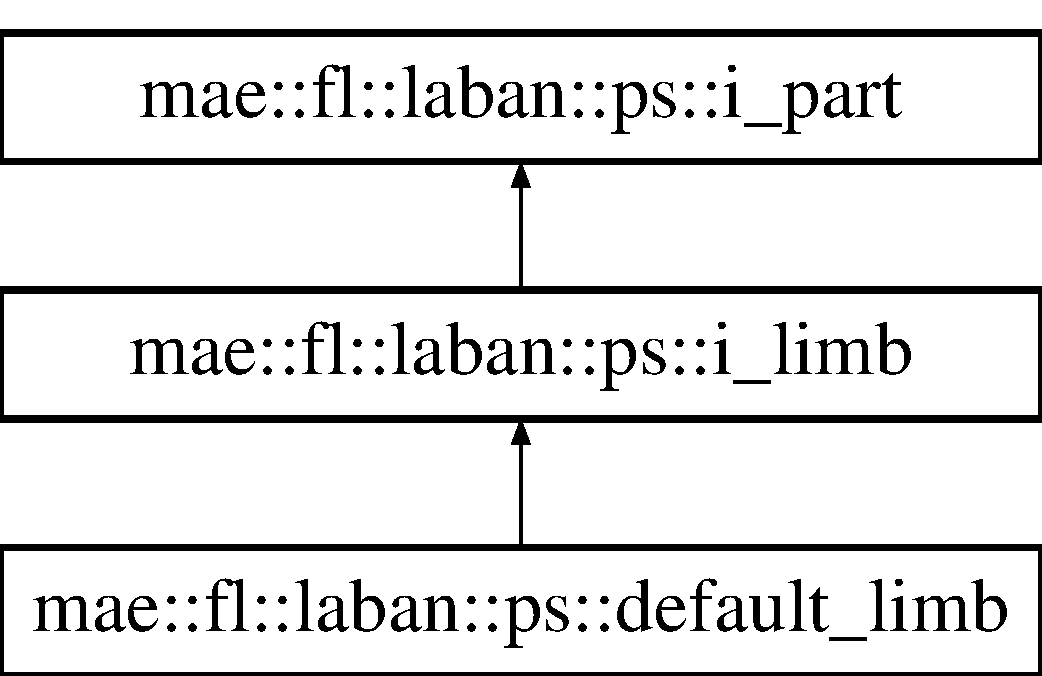
\includegraphics[height=3.000000cm]{classmae_1_1fl_1_1laban_1_1ps_1_1default__limb}
\end{center}
\end{figure}
\subsection*{Public Member Functions}
\begin{DoxyCompactItemize}
\item 
\hyperlink{classmae_1_1fl_1_1laban_1_1ps_1_1default__limb_ab153557aeb75d84a53698d10d4f5d883}{default\-\_\-limb} (e\-\_\-limb limb)
\item 
e\-\_\-limb \hyperlink{classmae_1_1fl_1_1laban_1_1ps_1_1default__limb_af92de65ffbed57d31534e3316baf0e91}{get\-\_\-limb} () const 
\item 
virtual std\-::string \hyperlink{classmae_1_1fl_1_1laban_1_1ps_1_1default__limb_a1d266ba068ce557431a90476b0ce3a82}{xml} (unsigned int indent=0, std\-::string namesp=\char`\"{}\char`\"{}) const 
\item 
virtual std\-::string \hyperlink{classmae_1_1fl_1_1laban_1_1ps_1_1default__limb_a489743d2be319dec0e05049b3c09db1e}{svg} (std\-::string identifier, double posx, double posy, double width, double height, bool left=false) const 
\item 
virtual bool \hyperlink{classmae_1_1fl_1_1laban_1_1ps_1_1default__limb_a9bdae13195e31e15c5511dcf04786aae}{equals} (std\-::shared\-\_\-ptr$<$ \hyperlink{classmae_1_1fl_1_1laban_1_1ps_1_1i__part}{i\-\_\-part} $>$ a) const 
\item 
virtual bool \hyperlink{classmae_1_1fl_1_1laban_1_1ps_1_1default__limb_ae7d58fdb145ee8c34b6f221ac0752b01}{equals} (std\-::shared\-\_\-ptr$<$ \hyperlink{classmae_1_1fl_1_1laban_1_1ps_1_1i__limb}{i\-\_\-limb} $>$ a) const 
\end{DoxyCompactItemize}


\subsection{Constructor \& Destructor Documentation}
\hypertarget{classmae_1_1fl_1_1laban_1_1ps_1_1default__limb_ab153557aeb75d84a53698d10d4f5d883}{\index{mae\-::fl\-::laban\-::ps\-::default\-\_\-limb@{mae\-::fl\-::laban\-::ps\-::default\-\_\-limb}!default\-\_\-limb@{default\-\_\-limb}}
\index{default\-\_\-limb@{default\-\_\-limb}!mae::fl::laban::ps::default_limb@{mae\-::fl\-::laban\-::ps\-::default\-\_\-limb}}
\subsubsection[{default\-\_\-limb}]{\setlength{\rightskip}{0pt plus 5cm}mae\-::fl\-::laban\-::ps\-::default\-\_\-limb\-::default\-\_\-limb (
\begin{DoxyParamCaption}
\item[{e\-\_\-limb}]{limb}
\end{DoxyParamCaption}
)}}\label{classmae_1_1fl_1_1laban_1_1ps_1_1default__limb_ab153557aeb75d84a53698d10d4f5d883}
Creates a default limb pre-\/sign which uses one of the defined limbs.


\begin{DoxyParams}{Parameters}
{\em limb} & The limb type. \\
\hline
\end{DoxyParams}


\subsection{Member Function Documentation}
\hypertarget{classmae_1_1fl_1_1laban_1_1ps_1_1default__limb_a9bdae13195e31e15c5511dcf04786aae}{\index{mae\-::fl\-::laban\-::ps\-::default\-\_\-limb@{mae\-::fl\-::laban\-::ps\-::default\-\_\-limb}!equals@{equals}}
\index{equals@{equals}!mae::fl::laban::ps::default_limb@{mae\-::fl\-::laban\-::ps\-::default\-\_\-limb}}
\subsubsection[{equals}]{\setlength{\rightskip}{0pt plus 5cm}bool mae\-::fl\-::laban\-::ps\-::default\-\_\-limb\-::equals (
\begin{DoxyParamCaption}
\item[{std\-::shared\-\_\-ptr$<$ {\bf i\-\_\-part} $>$}]{a}
\end{DoxyParamCaption}
) const\hspace{0.3cm}{\ttfamily [virtual]}}}\label{classmae_1_1fl_1_1laban_1_1ps_1_1default__limb_a9bdae13195e31e15c5511dcf04786aae}
Returns true if elements are equal.


\begin{DoxyParams}{Parameters}
{\em a} & The element to be compared to. \\
\hline
\end{DoxyParams}
\begin{DoxyReturn}{Returns}
True if equal. 
\end{DoxyReturn}


Implements \hyperlink{classmae_1_1fl_1_1laban_1_1ps_1_1i__limb_aa46cb4b952cc2a8692f3f32895a28041}{mae\-::fl\-::laban\-::ps\-::i\-\_\-limb}.

\hypertarget{classmae_1_1fl_1_1laban_1_1ps_1_1default__limb_ae7d58fdb145ee8c34b6f221ac0752b01}{\index{mae\-::fl\-::laban\-::ps\-::default\-\_\-limb@{mae\-::fl\-::laban\-::ps\-::default\-\_\-limb}!equals@{equals}}
\index{equals@{equals}!mae::fl::laban::ps::default_limb@{mae\-::fl\-::laban\-::ps\-::default\-\_\-limb}}
\subsubsection[{equals}]{\setlength{\rightskip}{0pt plus 5cm}bool mae\-::fl\-::laban\-::ps\-::default\-\_\-limb\-::equals (
\begin{DoxyParamCaption}
\item[{std\-::shared\-\_\-ptr$<$ {\bf i\-\_\-limb} $>$}]{a}
\end{DoxyParamCaption}
) const\hspace{0.3cm}{\ttfamily [virtual]}}}\label{classmae_1_1fl_1_1laban_1_1ps_1_1default__limb_ae7d58fdb145ee8c34b6f221ac0752b01}
Returns true if elements are equal.


\begin{DoxyParams}{Parameters}
{\em a} & The element to be compared to. \\
\hline
\end{DoxyParams}
\begin{DoxyReturn}{Returns}
True if equal. 
\end{DoxyReturn}


Implements \hyperlink{classmae_1_1fl_1_1laban_1_1ps_1_1i__limb_a7e7ba568e9711b8901234f2cb73b67b8}{mae\-::fl\-::laban\-::ps\-::i\-\_\-limb}.

\hypertarget{classmae_1_1fl_1_1laban_1_1ps_1_1default__limb_af92de65ffbed57d31534e3316baf0e91}{\index{mae\-::fl\-::laban\-::ps\-::default\-\_\-limb@{mae\-::fl\-::laban\-::ps\-::default\-\_\-limb}!get\-\_\-limb@{get\-\_\-limb}}
\index{get\-\_\-limb@{get\-\_\-limb}!mae::fl::laban::ps::default_limb@{mae\-::fl\-::laban\-::ps\-::default\-\_\-limb}}
\subsubsection[{get\-\_\-limb}]{\setlength{\rightskip}{0pt plus 5cm}e\-\_\-limb mae\-::fl\-::laban\-::ps\-::default\-\_\-limb\-::get\-\_\-limb (
\begin{DoxyParamCaption}
{}
\end{DoxyParamCaption}
) const}}\label{classmae_1_1fl_1_1laban_1_1ps_1_1default__limb_af92de65ffbed57d31534e3316baf0e91}
Returns the limb type.

\begin{DoxyReturn}{Returns}

\end{DoxyReturn}
\hypertarget{classmae_1_1fl_1_1laban_1_1ps_1_1default__limb_a489743d2be319dec0e05049b3c09db1e}{\index{mae\-::fl\-::laban\-::ps\-::default\-\_\-limb@{mae\-::fl\-::laban\-::ps\-::default\-\_\-limb}!svg@{svg}}
\index{svg@{svg}!mae::fl::laban::ps::default_limb@{mae\-::fl\-::laban\-::ps\-::default\-\_\-limb}}
\subsubsection[{svg}]{\setlength{\rightskip}{0pt plus 5cm}std\-::string mae\-::fl\-::laban\-::ps\-::default\-\_\-limb\-::svg (
\begin{DoxyParamCaption}
\item[{std\-::string}]{identifier, }
\item[{double}]{posx, }
\item[{double}]{posy, }
\item[{double}]{width, }
\item[{double}]{height, }
\item[{bool}]{left = {\ttfamily false}}
\end{DoxyParamCaption}
) const\hspace{0.3cm}{\ttfamily [virtual]}}}\label{classmae_1_1fl_1_1laban_1_1ps_1_1default__limb_a489743d2be319dec0e05049b3c09db1e}
Returns the S\-V\-G representation for this symbol.


\begin{DoxyParams}{Parameters}
{\em posx} & The x position. \\
\hline
{\em posy} & The y position. \\
\hline
{\em width} & The width. \\
\hline
{\em height} & The height. \\
\hline
\end{DoxyParams}
\begin{DoxyReturn}{Returns}
The S\-V\-G. 
\end{DoxyReturn}


Implements \hyperlink{classmae_1_1fl_1_1laban_1_1ps_1_1i__part_a78227d5ecd87655a7a9454c68f470368}{mae\-::fl\-::laban\-::ps\-::i\-\_\-part}.

\hypertarget{classmae_1_1fl_1_1laban_1_1ps_1_1default__limb_a1d266ba068ce557431a90476b0ce3a82}{\index{mae\-::fl\-::laban\-::ps\-::default\-\_\-limb@{mae\-::fl\-::laban\-::ps\-::default\-\_\-limb}!xml@{xml}}
\index{xml@{xml}!mae::fl::laban::ps::default_limb@{mae\-::fl\-::laban\-::ps\-::default\-\_\-limb}}
\subsubsection[{xml}]{\setlength{\rightskip}{0pt plus 5cm}std\-::string mae\-::fl\-::laban\-::ps\-::default\-\_\-limb\-::xml (
\begin{DoxyParamCaption}
\item[{unsigned int}]{indent = {\ttfamily 0}, }
\item[{std\-::string}]{namesp = {\ttfamily \char`\"{}\char`\"{}}}
\end{DoxyParamCaption}
) const\hspace{0.3cm}{\ttfamily [virtual]}}}\label{classmae_1_1fl_1_1laban_1_1ps_1_1default__limb_a1d266ba068ce557431a90476b0ce3a82}
Returns the X\-M\-L representation for this element.


\begin{DoxyParams}{Parameters}
{\em indent} & The applied indent. \\
\hline
{\em namesp} & The prefixed X\-M\-L namespace.\\
\hline
\end{DoxyParams}
\begin{DoxyReturn}{Returns}
The X\-M\-L string. 
\end{DoxyReturn}


Implements \hyperlink{classmae_1_1fl_1_1laban_1_1ps_1_1i__limb_a7a5c3ca32936748a1e60fdab1d29b1c9}{mae\-::fl\-::laban\-::ps\-::i\-\_\-limb}.



The documentation for this class was generated from the following files\-:\begin{DoxyCompactItemize}
\item 
src/mae/fl/laban/ps/default\-\_\-limb.\-hpp\item 
src/mae/fl/laban/ps/default\-\_\-limb.\-cpp\end{DoxyCompactItemize}

\hypertarget{classmae_1_1fl_1_1laban_1_1ps_1_1digit__part}{\section{mae\-:\-:fl\-:\-:laban\-:\-:ps\-:\-:digit\-\_\-part Class Reference}
\label{classmae_1_1fl_1_1laban_1_1ps_1_1digit__part}\index{mae\-::fl\-::laban\-::ps\-::digit\-\_\-part@{mae\-::fl\-::laban\-::ps\-::digit\-\_\-part}}
}
Inheritance diagram for mae\-:\-:fl\-:\-:laban\-:\-:ps\-:\-:digit\-\_\-part\-:\begin{figure}[H]
\begin{center}
\leavevmode
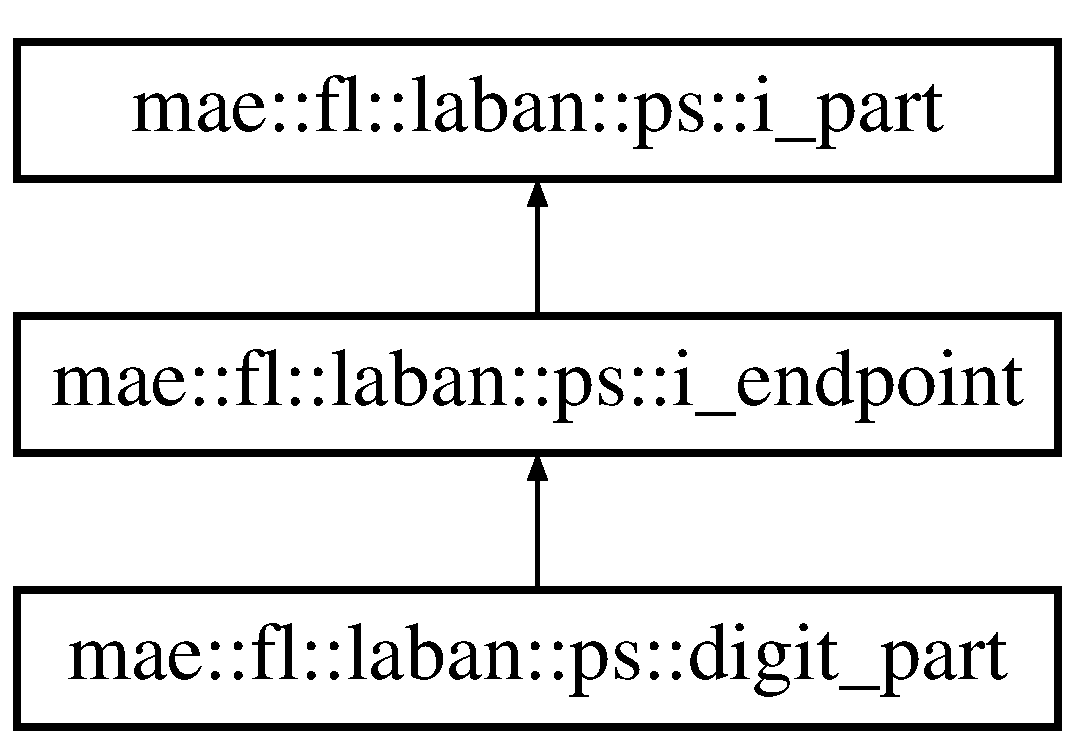
\includegraphics[height=3.000000cm]{classmae_1_1fl_1_1laban_1_1ps_1_1digit__part}
\end{center}
\end{figure}
\subsection*{Public Member Functions}
\begin{DoxyCompactItemize}
\item 
\hyperlink{classmae_1_1fl_1_1laban_1_1ps_1_1digit__part_a4f81dd510be4efc56b501edf7eb57ecf}{digit\-\_\-part} (e\-\_\-digit digit, unsigned int knuckle)
\item 
e\-\_\-digit \hyperlink{classmae_1_1fl_1_1laban_1_1ps_1_1digit__part_a1e0d08a914859b24ffbabec5bd9f87a8}{get\-\_\-digit} () const 
\item 
unsigned int \hyperlink{classmae_1_1fl_1_1laban_1_1ps_1_1digit__part_a50eba0820368e7315d84f3782238e646}{get\-\_\-knuckle} () const 
\item 
virtual std\-::string \hyperlink{classmae_1_1fl_1_1laban_1_1ps_1_1digit__part_a51e9b056b0d57310e1423efbf8ebec48}{xml} (unsigned int indent=0, std\-::string namesp=\char`\"{}\char`\"{}) const 
\item 
virtual std\-::string \hyperlink{classmae_1_1fl_1_1laban_1_1ps_1_1digit__part_a4f9204b03aaf808940d32d1b6a3ea325}{svg} (std\-::string identifier, double posx, double posy, double width, double height, bool left=false) const 
\item 
virtual std\-::shared\-\_\-ptr\\*
$<$ \hyperlink{classmae_1_1fl_1_1laban_1_1ps_1_1i__endpoint}{i\-\_\-endpoint} $>$ \hyperlink{classmae_1_1fl_1_1laban_1_1ps_1_1digit__part_ad8f600cbaccf7194ea70c93432a1e9b5}{get\-\_\-fixed\-\_\-end} () const 
\item 
virtual bool \hyperlink{classmae_1_1fl_1_1laban_1_1ps_1_1digit__part_a6bcdd921e55c60908e827534d4957c4d}{equals} (std\-::shared\-\_\-ptr$<$ \hyperlink{classmae_1_1fl_1_1laban_1_1ps_1_1i__part}{i\-\_\-part} $>$ a) const 
\item 
virtual bool \hyperlink{classmae_1_1fl_1_1laban_1_1ps_1_1digit__part_a0966a987076279fe198566b953bbc7a3}{equals} (std\-::shared\-\_\-ptr$<$ \hyperlink{classmae_1_1fl_1_1laban_1_1ps_1_1i__endpoint}{i\-\_\-endpoint} $>$ a) const 
\end{DoxyCompactItemize}


\subsection{Constructor \& Destructor Documentation}
\hypertarget{classmae_1_1fl_1_1laban_1_1ps_1_1digit__part_a4f81dd510be4efc56b501edf7eb57ecf}{\index{mae\-::fl\-::laban\-::ps\-::digit\-\_\-part@{mae\-::fl\-::laban\-::ps\-::digit\-\_\-part}!digit\-\_\-part@{digit\-\_\-part}}
\index{digit\-\_\-part@{digit\-\_\-part}!mae::fl::laban::ps::digit_part@{mae\-::fl\-::laban\-::ps\-::digit\-\_\-part}}
\subsubsection[{digit\-\_\-part}]{\setlength{\rightskip}{0pt plus 5cm}mae\-::fl\-::laban\-::ps\-::digit\-\_\-part\-::digit\-\_\-part (
\begin{DoxyParamCaption}
\item[{e\-\_\-digit}]{digit, }
\item[{unsigned int}]{knuckle}
\end{DoxyParamCaption}
)}}\label{classmae_1_1fl_1_1laban_1_1ps_1_1digit__part_a4f81dd510be4efc56b501edf7eb57ecf}
Creates a digit pre-\/sign which consist of a digit (finger or toes) and a knuckle.


\begin{DoxyParams}{Parameters}
{\em digit} & The addressed digit. \\
\hline
{\em knuckle} & The addressed knuckle. Zero represents the whole digit, whereas A number represents the knuckle counted from the base. Therefore 3 for toes and 4 for fingers is the maximum valid value. \\
\hline
\end{DoxyParams}


\subsection{Member Function Documentation}
\hypertarget{classmae_1_1fl_1_1laban_1_1ps_1_1digit__part_a6bcdd921e55c60908e827534d4957c4d}{\index{mae\-::fl\-::laban\-::ps\-::digit\-\_\-part@{mae\-::fl\-::laban\-::ps\-::digit\-\_\-part}!equals@{equals}}
\index{equals@{equals}!mae::fl::laban::ps::digit_part@{mae\-::fl\-::laban\-::ps\-::digit\-\_\-part}}
\subsubsection[{equals}]{\setlength{\rightskip}{0pt plus 5cm}bool mae\-::fl\-::laban\-::ps\-::digit\-\_\-part\-::equals (
\begin{DoxyParamCaption}
\item[{std\-::shared\-\_\-ptr$<$ {\bf i\-\_\-part} $>$}]{a}
\end{DoxyParamCaption}
) const\hspace{0.3cm}{\ttfamily [virtual]}}}\label{classmae_1_1fl_1_1laban_1_1ps_1_1digit__part_a6bcdd921e55c60908e827534d4957c4d}
Returns true if elements are equal.


\begin{DoxyParams}{Parameters}
{\em a} & The element to be compared to. \\
\hline
\end{DoxyParams}
\begin{DoxyReturn}{Returns}
True if equal. 
\end{DoxyReturn}


Implements \hyperlink{classmae_1_1fl_1_1laban_1_1ps_1_1i__endpoint_abc675b07d3ce69fbec362b2e792a1e06}{mae\-::fl\-::laban\-::ps\-::i\-\_\-endpoint}.

\hypertarget{classmae_1_1fl_1_1laban_1_1ps_1_1digit__part_a0966a987076279fe198566b953bbc7a3}{\index{mae\-::fl\-::laban\-::ps\-::digit\-\_\-part@{mae\-::fl\-::laban\-::ps\-::digit\-\_\-part}!equals@{equals}}
\index{equals@{equals}!mae::fl::laban::ps::digit_part@{mae\-::fl\-::laban\-::ps\-::digit\-\_\-part}}
\subsubsection[{equals}]{\setlength{\rightskip}{0pt plus 5cm}bool mae\-::fl\-::laban\-::ps\-::digit\-\_\-part\-::equals (
\begin{DoxyParamCaption}
\item[{std\-::shared\-\_\-ptr$<$ {\bf i\-\_\-endpoint} $>$}]{a}
\end{DoxyParamCaption}
) const\hspace{0.3cm}{\ttfamily [virtual]}}}\label{classmae_1_1fl_1_1laban_1_1ps_1_1digit__part_a0966a987076279fe198566b953bbc7a3}
Returns true if elements are equal.


\begin{DoxyParams}{Parameters}
{\em a} & The element to be compared to. \\
\hline
\end{DoxyParams}
\begin{DoxyReturn}{Returns}
True if equal. 
\end{DoxyReturn}


Implements \hyperlink{classmae_1_1fl_1_1laban_1_1ps_1_1i__endpoint_aeffb14c43728d2ef094122f3d0278455}{mae\-::fl\-::laban\-::ps\-::i\-\_\-endpoint}.

\hypertarget{classmae_1_1fl_1_1laban_1_1ps_1_1digit__part_a1e0d08a914859b24ffbabec5bd9f87a8}{\index{mae\-::fl\-::laban\-::ps\-::digit\-\_\-part@{mae\-::fl\-::laban\-::ps\-::digit\-\_\-part}!get\-\_\-digit@{get\-\_\-digit}}
\index{get\-\_\-digit@{get\-\_\-digit}!mae::fl::laban::ps::digit_part@{mae\-::fl\-::laban\-::ps\-::digit\-\_\-part}}
\subsubsection[{get\-\_\-digit}]{\setlength{\rightskip}{0pt plus 5cm}e\-\_\-digit mae\-::fl\-::laban\-::ps\-::digit\-\_\-part\-::get\-\_\-digit (
\begin{DoxyParamCaption}
{}
\end{DoxyParamCaption}
) const}}\label{classmae_1_1fl_1_1laban_1_1ps_1_1digit__part_a1e0d08a914859b24ffbabec5bd9f87a8}
Returns the addressed digit.

\begin{DoxyReturn}{Returns}

\end{DoxyReturn}
\hypertarget{classmae_1_1fl_1_1laban_1_1ps_1_1digit__part_ad8f600cbaccf7194ea70c93432a1e9b5}{\index{mae\-::fl\-::laban\-::ps\-::digit\-\_\-part@{mae\-::fl\-::laban\-::ps\-::digit\-\_\-part}!get\-\_\-fixed\-\_\-end@{get\-\_\-fixed\-\_\-end}}
\index{get\-\_\-fixed\-\_\-end@{get\-\_\-fixed\-\_\-end}!mae::fl::laban::ps::digit_part@{mae\-::fl\-::laban\-::ps\-::digit\-\_\-part}}
\subsubsection[{get\-\_\-fixed\-\_\-end}]{\setlength{\rightskip}{0pt plus 5cm}std\-::shared\-\_\-ptr$<$ {\bf i\-\_\-endpoint} $>$ mae\-::fl\-::laban\-::ps\-::digit\-\_\-part\-::get\-\_\-fixed\-\_\-end (
\begin{DoxyParamCaption}
{}
\end{DoxyParamCaption}
) const\hspace{0.3cm}{\ttfamily [virtual]}}}\label{classmae_1_1fl_1_1laban_1_1ps_1_1digit__part_ad8f600cbaccf7194ea70c93432a1e9b5}
Returns the predecessor of the current endpoint (which is the default fixed endpoint). If the endpoint is the beginning of the extremity null is returned.

If the base knuckle is zero, the hand or foot (joint part) is returned.

\begin{DoxyReturn}{Returns}
The successor element. 
\end{DoxyReturn}


Implements \hyperlink{classmae_1_1fl_1_1laban_1_1ps_1_1i__endpoint_a0938824cc5892b072636c3b52352b3f2}{mae\-::fl\-::laban\-::ps\-::i\-\_\-endpoint}.

\hypertarget{classmae_1_1fl_1_1laban_1_1ps_1_1digit__part_a50eba0820368e7315d84f3782238e646}{\index{mae\-::fl\-::laban\-::ps\-::digit\-\_\-part@{mae\-::fl\-::laban\-::ps\-::digit\-\_\-part}!get\-\_\-knuckle@{get\-\_\-knuckle}}
\index{get\-\_\-knuckle@{get\-\_\-knuckle}!mae::fl::laban::ps::digit_part@{mae\-::fl\-::laban\-::ps\-::digit\-\_\-part}}
\subsubsection[{get\-\_\-knuckle}]{\setlength{\rightskip}{0pt plus 5cm}unsigned int mae\-::fl\-::laban\-::ps\-::digit\-\_\-part\-::get\-\_\-knuckle (
\begin{DoxyParamCaption}
{}
\end{DoxyParamCaption}
) const}}\label{classmae_1_1fl_1_1laban_1_1ps_1_1digit__part_a50eba0820368e7315d84f3782238e646}
Returns the addressed knuckle. Zero represents the whole digit whereas a number represents the knuckle counted from the base.

\begin{DoxyReturn}{Returns}

\end{DoxyReturn}
\hypertarget{classmae_1_1fl_1_1laban_1_1ps_1_1digit__part_a4f9204b03aaf808940d32d1b6a3ea325}{\index{mae\-::fl\-::laban\-::ps\-::digit\-\_\-part@{mae\-::fl\-::laban\-::ps\-::digit\-\_\-part}!svg@{svg}}
\index{svg@{svg}!mae::fl::laban::ps::digit_part@{mae\-::fl\-::laban\-::ps\-::digit\-\_\-part}}
\subsubsection[{svg}]{\setlength{\rightskip}{0pt plus 5cm}std\-::string mae\-::fl\-::laban\-::ps\-::digit\-\_\-part\-::svg (
\begin{DoxyParamCaption}
\item[{std\-::string}]{identifier, }
\item[{double}]{posx, }
\item[{double}]{posy, }
\item[{double}]{width, }
\item[{double}]{height, }
\item[{bool}]{left = {\ttfamily false}}
\end{DoxyParamCaption}
) const\hspace{0.3cm}{\ttfamily [virtual]}}}\label{classmae_1_1fl_1_1laban_1_1ps_1_1digit__part_a4f9204b03aaf808940d32d1b6a3ea325}
Returns the S\-V\-G representation for this symbol.


\begin{DoxyParams}{Parameters}
{\em posx} & The x position. \\
\hline
{\em posy} & The y position. \\
\hline
{\em width} & The width. \\
\hline
{\em height} & The height. \\
\hline
\end{DoxyParams}
\begin{DoxyReturn}{Returns}
The S\-V\-G. 
\end{DoxyReturn}


Implements \hyperlink{classmae_1_1fl_1_1laban_1_1ps_1_1i__part_a78227d5ecd87655a7a9454c68f470368}{mae\-::fl\-::laban\-::ps\-::i\-\_\-part}.

\hypertarget{classmae_1_1fl_1_1laban_1_1ps_1_1digit__part_a51e9b056b0d57310e1423efbf8ebec48}{\index{mae\-::fl\-::laban\-::ps\-::digit\-\_\-part@{mae\-::fl\-::laban\-::ps\-::digit\-\_\-part}!xml@{xml}}
\index{xml@{xml}!mae::fl::laban::ps::digit_part@{mae\-::fl\-::laban\-::ps\-::digit\-\_\-part}}
\subsubsection[{xml}]{\setlength{\rightskip}{0pt plus 5cm}std\-::string mae\-::fl\-::laban\-::ps\-::digit\-\_\-part\-::xml (
\begin{DoxyParamCaption}
\item[{unsigned int}]{indent = {\ttfamily 0}, }
\item[{std\-::string}]{namesp = {\ttfamily \char`\"{}\char`\"{}}}
\end{DoxyParamCaption}
) const\hspace{0.3cm}{\ttfamily [virtual]}}}\label{classmae_1_1fl_1_1laban_1_1ps_1_1digit__part_a51e9b056b0d57310e1423efbf8ebec48}
Returns the X\-M\-L representation for this element.


\begin{DoxyParams}{Parameters}
{\em indent} & The applied indent. \\
\hline
{\em namesp} & The prefixed X\-M\-L namespace.\\
\hline
\end{DoxyParams}
\begin{DoxyReturn}{Returns}
The X\-M\-L string. 
\end{DoxyReturn}


Implements \hyperlink{classmae_1_1fl_1_1laban_1_1ps_1_1i__endpoint_a1af7dbd05400cbdd7f9f45ef75dd38d6}{mae\-::fl\-::laban\-::ps\-::i\-\_\-endpoint}.



The documentation for this class was generated from the following files\-:\begin{DoxyCompactItemize}
\item 
src/mae/fl/laban/ps/digit\-\_\-part.\-hpp\item 
src/mae/fl/laban/ps/digit\-\_\-part.\-cpp\end{DoxyCompactItemize}

\hypertarget{classmae_1_1fl_1_1laban_1_1mv_1_1direction__symbol}{\section{mae\-:\-:fl\-:\-:laban\-:\-:mv\-:\-:direction\-\_\-symbol Class Reference}
\label{classmae_1_1fl_1_1laban_1_1mv_1_1direction__symbol}\index{mae\-::fl\-::laban\-::mv\-::direction\-\_\-symbol@{mae\-::fl\-::laban\-::mv\-::direction\-\_\-symbol}}
}
Inheritance diagram for mae\-:\-:fl\-:\-:laban\-:\-:mv\-:\-:direction\-\_\-symbol\-:\begin{figure}[H]
\begin{center}
\leavevmode
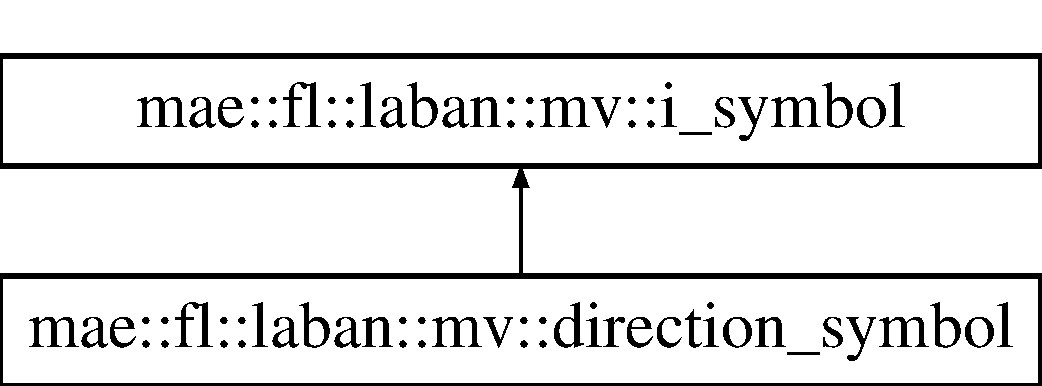
\includegraphics[height=2.000000cm]{classmae_1_1fl_1_1laban_1_1mv_1_1direction__symbol}
\end{center}
\end{figure}
\subsection*{Public Member Functions}
\begin{DoxyCompactItemize}
\item 
\hyperlink{classmae_1_1fl_1_1laban_1_1mv_1_1direction__symbol_abae9d91d2b0448e8aaa5a8b427f029f7}{direction\-\_\-symbol} (e\-\_\-level vertical, e\-\_\-direction horizontal, std\-::shared\-\_\-ptr$<$ \hyperlink{classmae_1_1fl_1_1laban_1_1mv_1_1pin}{pin} $>$ modification\-\_\-pin=nullptr, std\-::shared\-\_\-ptr$<$ \hyperlink{classmae_1_1fl_1_1laban_1_1mv_1_1pin}{pin} $>$ relationship\-\_\-pin=nullptr, std\-::shared\-\_\-ptr$<$ \hyperlink{classmae_1_1fl_1_1laban_1_1mv_1_1i__dynamics__sign}{i\-\_\-dynamics\-\_\-sign} $>$ dynamics=nullptr, std\-::shared\-\_\-ptr$<$ \hyperlink{classmae_1_1fl_1_1laban_1_1mv_1_1space__measurement}{space\-\_\-measurement} $>$ \hyperlink{classmae_1_1fl_1_1laban_1_1mv_1_1space__measurement}{space\-\_\-measurement}=nullptr, e\-\_\-contact\-\_\-hook contact\-\_\-hook=e\-\_\-contact\-\_\-hook\-::\-N\-O\-N\-E\-\_\-\-C\-O\-N\-T\-A\-C\-T\-\_\-\-H\-O\-O\-K)
\item 
e\-\_\-level \hyperlink{classmae_1_1fl_1_1laban_1_1mv_1_1direction__symbol_a0d80aa6b7d1d8cdd5cf3df033c680148}{get\-\_\-vertical} () const 
\item 
e\-\_\-direction \hyperlink{classmae_1_1fl_1_1laban_1_1mv_1_1direction__symbol_aab2d3a4913b21e664e5b6d52c551568e}{get\-\_\-horizontal} () const 
\item 
std\-::shared\-\_\-ptr$<$ \hyperlink{classmae_1_1fl_1_1laban_1_1mv_1_1pin}{pin} $>$ \hyperlink{classmae_1_1fl_1_1laban_1_1mv_1_1direction__symbol_a00fe8b9674d324ad875a69b4621ce4a6}{get\-\_\-modification\-\_\-pin} () const 
\item 
std\-::shared\-\_\-ptr$<$ \hyperlink{classmae_1_1fl_1_1laban_1_1mv_1_1pin}{pin} $>$ \hyperlink{classmae_1_1fl_1_1laban_1_1mv_1_1direction__symbol_a2c709125f5108e611cc971e4eff4ba61}{get\-\_\-relationship\-\_\-pin} () const 
\item 
std\-::shared\-\_\-ptr$<$ \hyperlink{classmae_1_1fl_1_1laban_1_1mv_1_1i__dynamics__sign}{i\-\_\-dynamics\-\_\-sign} $>$ \hyperlink{classmae_1_1fl_1_1laban_1_1mv_1_1direction__symbol_a298ccff5d107bef2359f485f17dd08f8}{get\-\_\-dynamics} () const 
\item 
std\-::shared\-\_\-ptr\\*
$<$ \hyperlink{classmae_1_1fl_1_1laban_1_1mv_1_1space__measurement}{space\-\_\-measurement} $>$ \hyperlink{classmae_1_1fl_1_1laban_1_1mv_1_1direction__symbol_a0c57ad8ba8bb6502c42155fc2f5a2708}{get\-\_\-space\-\_\-measurement} () const 
\item 
e\-\_\-contact\-\_\-hook \hyperlink{classmae_1_1fl_1_1laban_1_1mv_1_1direction__symbol_aa19b098d88f1d052436b2c4be877d38a}{get\-\_\-contact\-\_\-hook} () const 
\item 
virtual bool \hyperlink{classmae_1_1fl_1_1laban_1_1mv_1_1direction__symbol_a2ea85fd4be221d8dc2da7ee417dd829c}{equals} (std\-::shared\-\_\-ptr$<$ \hyperlink{classmae_1_1fl_1_1laban_1_1mv_1_1i__symbol}{i\-\_\-symbol} $>$ a) const 
\item 
virtual std\-::string \hyperlink{classmae_1_1fl_1_1laban_1_1mv_1_1direction__symbol_a987e147f6a6ae37e50d450f382d850c1}{xml} (unsigned int indent=0, std\-::string namesp=\char`\"{}\char`\"{}) const 
\item 
virtual std\-::string \hyperlink{classmae_1_1fl_1_1laban_1_1mv_1_1direction__symbol_af0e41f900f48beafee3e8daeade9687e}{svg} (std\-::string identifier, double posx, double posy, double width, double height, bool left=false) const 
\item 
virtual std\-::string \hyperlink{classmae_1_1fl_1_1laban_1_1mv_1_1direction__symbol_a3d6beaca72898fa289efd8dfc7e283f7}{str} () const 
\end{DoxyCompactItemize}
\subsection*{Friends}
\begin{DoxyCompactItemize}
\item 
\hypertarget{classmae_1_1fl_1_1laban_1_1mv_1_1direction__symbol_a16a89647391c8b8ffee475f535b8380b}{std\-::ostream \& {\bfseries operator$<$$<$} (std\-::ostream \&os, const \hyperlink{classmae_1_1fl_1_1laban_1_1mv_1_1direction__symbol}{direction\-\_\-symbol} \&obj)}\label{classmae_1_1fl_1_1laban_1_1mv_1_1direction__symbol_a16a89647391c8b8ffee475f535b8380b}

\item 
\hypertarget{classmae_1_1fl_1_1laban_1_1mv_1_1direction__symbol_a7777346ab8e477f0dbb9706babefe05c}{std\-::ostream \& {\bfseries operator$<$$<$} (std\-::ostream \&os, const std\-::shared\-\_\-ptr$<$ \hyperlink{classmae_1_1fl_1_1laban_1_1mv_1_1direction__symbol}{direction\-\_\-symbol} $>$ \&obj)}\label{classmae_1_1fl_1_1laban_1_1mv_1_1direction__symbol_a7777346ab8e477f0dbb9706babefe05c}

\end{DoxyCompactItemize}


\subsection{Constructor \& Destructor Documentation}
\hypertarget{classmae_1_1fl_1_1laban_1_1mv_1_1direction__symbol_abae9d91d2b0448e8aaa5a8b427f029f7}{\index{mae\-::fl\-::laban\-::mv\-::direction\-\_\-symbol@{mae\-::fl\-::laban\-::mv\-::direction\-\_\-symbol}!direction\-\_\-symbol@{direction\-\_\-symbol}}
\index{direction\-\_\-symbol@{direction\-\_\-symbol}!mae::fl::laban::mv::direction_symbol@{mae\-::fl\-::laban\-::mv\-::direction\-\_\-symbol}}
\subsubsection[{direction\-\_\-symbol}]{\setlength{\rightskip}{0pt plus 5cm}mae\-::fl\-::laban\-::mv\-::direction\-\_\-symbol\-::direction\-\_\-symbol (
\begin{DoxyParamCaption}
\item[{e\-\_\-level}]{vertical, }
\item[{e\-\_\-direction}]{horizontal, }
\item[{std\-::shared\-\_\-ptr$<$ {\bf pin} $>$}]{modification\-\_\-pin = {\ttfamily nullptr}, }
\item[{std\-::shared\-\_\-ptr$<$ {\bf pin} $>$}]{relationship\-\_\-pin = {\ttfamily nullptr}, }
\item[{std\-::shared\-\_\-ptr$<$ {\bf i\-\_\-dynamics\-\_\-sign} $>$}]{dynamics = {\ttfamily nullptr}, }
\item[{std\-::shared\-\_\-ptr$<$ {\bf space\-\_\-measurement} $>$}]{space\-\_\-measurement = {\ttfamily nullptr}, }
\item[{e\-\_\-contact\-\_\-hook}]{contact\-\_\-hook = {\ttfamily e\-\_\-contact\-\_\-hook\-:\-:NONE\-\_\-CONTACT\-\_\-HOOK}}
\end{DoxyParamCaption}
)}}\label{classmae_1_1fl_1_1laban_1_1mv_1_1direction__symbol_abae9d91d2b0448e8aaa5a8b427f029f7}
Creates a direction symbol.


\begin{DoxyParams}{Parameters}
{\em vertical} & The level of this symbol. \\
\hline
{\em horizontal} & The (horizontal) direction of this symbol. \\
\hline
{\em modification\-\_\-pin} & (optional) A modification pin. \\
\hline
{\em relationship\-\_\-pin} & (optional) A relationship pin. \\
\hline
{\em dynamics} & (optional) A dynamics sign. \\
\hline
{\em \hyperlink{classmae_1_1fl_1_1laban_1_1mv_1_1space__measurement}{space\-\_\-measurement}} & (optional) A space measurement sign. \\
\hline
{\em contact\-\_\-hook} & (optional) The contact hook. \\
\hline
\end{DoxyParams}


\subsection{Member Function Documentation}
\hypertarget{classmae_1_1fl_1_1laban_1_1mv_1_1direction__symbol_a2ea85fd4be221d8dc2da7ee417dd829c}{\index{mae\-::fl\-::laban\-::mv\-::direction\-\_\-symbol@{mae\-::fl\-::laban\-::mv\-::direction\-\_\-symbol}!equals@{equals}}
\index{equals@{equals}!mae::fl::laban::mv::direction_symbol@{mae\-::fl\-::laban\-::mv\-::direction\-\_\-symbol}}
\subsubsection[{equals}]{\setlength{\rightskip}{0pt plus 5cm}bool mae\-::fl\-::laban\-::mv\-::direction\-\_\-symbol\-::equals (
\begin{DoxyParamCaption}
\item[{std\-::shared\-\_\-ptr$<$ {\bf i\-\_\-symbol} $>$}]{a}
\end{DoxyParamCaption}
) const\hspace{0.3cm}{\ttfamily [virtual]}}}\label{classmae_1_1fl_1_1laban_1_1mv_1_1direction__symbol_a2ea85fd4be221d8dc2da7ee417dd829c}
Returns true if signs are equal.


\begin{DoxyParams}{Parameters}
{\em a} & The sign to be compared to. \\
\hline
\end{DoxyParams}
\begin{DoxyReturn}{Returns}
True if equal. 
\end{DoxyReturn}


Implements \hyperlink{classmae_1_1fl_1_1laban_1_1mv_1_1i__symbol_a78d90af5e1da4a6561d7545a76689d0e}{mae\-::fl\-::laban\-::mv\-::i\-\_\-symbol}.

\hypertarget{classmae_1_1fl_1_1laban_1_1mv_1_1direction__symbol_aa19b098d88f1d052436b2c4be877d38a}{\index{mae\-::fl\-::laban\-::mv\-::direction\-\_\-symbol@{mae\-::fl\-::laban\-::mv\-::direction\-\_\-symbol}!get\-\_\-contact\-\_\-hook@{get\-\_\-contact\-\_\-hook}}
\index{get\-\_\-contact\-\_\-hook@{get\-\_\-contact\-\_\-hook}!mae::fl::laban::mv::direction_symbol@{mae\-::fl\-::laban\-::mv\-::direction\-\_\-symbol}}
\subsubsection[{get\-\_\-contact\-\_\-hook}]{\setlength{\rightskip}{0pt plus 5cm}e\-\_\-contact\-\_\-hook mae\-::fl\-::laban\-::mv\-::direction\-\_\-symbol\-::get\-\_\-contact\-\_\-hook (
\begin{DoxyParamCaption}
{}
\end{DoxyParamCaption}
) const}}\label{classmae_1_1fl_1_1laban_1_1mv_1_1direction__symbol_aa19b098d88f1d052436b2c4be877d38a}
Returns the contact hook. Contact hook is set to N\-O\-N\-E if unused.

\begin{DoxyReturn}{Returns}
The contact hook. 
\end{DoxyReturn}
\hypertarget{classmae_1_1fl_1_1laban_1_1mv_1_1direction__symbol_a298ccff5d107bef2359f485f17dd08f8}{\index{mae\-::fl\-::laban\-::mv\-::direction\-\_\-symbol@{mae\-::fl\-::laban\-::mv\-::direction\-\_\-symbol}!get\-\_\-dynamics@{get\-\_\-dynamics}}
\index{get\-\_\-dynamics@{get\-\_\-dynamics}!mae::fl::laban::mv::direction_symbol@{mae\-::fl\-::laban\-::mv\-::direction\-\_\-symbol}}
\subsubsection[{get\-\_\-dynamics}]{\setlength{\rightskip}{0pt plus 5cm}std\-::shared\-\_\-ptr$<$ {\bf i\-\_\-dynamics\-\_\-sign} $>$ mae\-::fl\-::laban\-::mv\-::direction\-\_\-symbol\-::get\-\_\-dynamics (
\begin{DoxyParamCaption}
{}
\end{DoxyParamCaption}
) const}}\label{classmae_1_1fl_1_1laban_1_1mv_1_1direction__symbol_a298ccff5d107bef2359f485f17dd08f8}
Returns the dynamics sign if any. Returns null otherwise.

\begin{DoxyReturn}{Returns}
A shared pointer to the dynamics sign. 
\end{DoxyReturn}
\hypertarget{classmae_1_1fl_1_1laban_1_1mv_1_1direction__symbol_aab2d3a4913b21e664e5b6d52c551568e}{\index{mae\-::fl\-::laban\-::mv\-::direction\-\_\-symbol@{mae\-::fl\-::laban\-::mv\-::direction\-\_\-symbol}!get\-\_\-horizontal@{get\-\_\-horizontal}}
\index{get\-\_\-horizontal@{get\-\_\-horizontal}!mae::fl::laban::mv::direction_symbol@{mae\-::fl\-::laban\-::mv\-::direction\-\_\-symbol}}
\subsubsection[{get\-\_\-horizontal}]{\setlength{\rightskip}{0pt plus 5cm}e\-\_\-direction mae\-::fl\-::laban\-::mv\-::direction\-\_\-symbol\-::get\-\_\-horizontal (
\begin{DoxyParamCaption}
{}
\end{DoxyParamCaption}
) const}}\label{classmae_1_1fl_1_1laban_1_1mv_1_1direction__symbol_aab2d3a4913b21e664e5b6d52c551568e}
Returns the (horizontal) direction of this symbol.

\begin{DoxyReturn}{Returns}
The direction. 
\end{DoxyReturn}
\hypertarget{classmae_1_1fl_1_1laban_1_1mv_1_1direction__symbol_a00fe8b9674d324ad875a69b4621ce4a6}{\index{mae\-::fl\-::laban\-::mv\-::direction\-\_\-symbol@{mae\-::fl\-::laban\-::mv\-::direction\-\_\-symbol}!get\-\_\-modification\-\_\-pin@{get\-\_\-modification\-\_\-pin}}
\index{get\-\_\-modification\-\_\-pin@{get\-\_\-modification\-\_\-pin}!mae::fl::laban::mv::direction_symbol@{mae\-::fl\-::laban\-::mv\-::direction\-\_\-symbol}}
\subsubsection[{get\-\_\-modification\-\_\-pin}]{\setlength{\rightskip}{0pt plus 5cm}std\-::shared\-\_\-ptr$<$ {\bf pin} $>$ mae\-::fl\-::laban\-::mv\-::direction\-\_\-symbol\-::get\-\_\-modification\-\_\-pin (
\begin{DoxyParamCaption}
{}
\end{DoxyParamCaption}
) const}}\label{classmae_1_1fl_1_1laban_1_1mv_1_1direction__symbol_a00fe8b9674d324ad875a69b4621ce4a6}
Returns the applied modification pin if any. Returns null otherwise.

\begin{DoxyReturn}{Returns}
A shared pointer to the pin. 
\end{DoxyReturn}
\hypertarget{classmae_1_1fl_1_1laban_1_1mv_1_1direction__symbol_a2c709125f5108e611cc971e4eff4ba61}{\index{mae\-::fl\-::laban\-::mv\-::direction\-\_\-symbol@{mae\-::fl\-::laban\-::mv\-::direction\-\_\-symbol}!get\-\_\-relationship\-\_\-pin@{get\-\_\-relationship\-\_\-pin}}
\index{get\-\_\-relationship\-\_\-pin@{get\-\_\-relationship\-\_\-pin}!mae::fl::laban::mv::direction_symbol@{mae\-::fl\-::laban\-::mv\-::direction\-\_\-symbol}}
\subsubsection[{get\-\_\-relationship\-\_\-pin}]{\setlength{\rightskip}{0pt plus 5cm}std\-::shared\-\_\-ptr$<$ {\bf pin} $>$ mae\-::fl\-::laban\-::mv\-::direction\-\_\-symbol\-::get\-\_\-relationship\-\_\-pin (
\begin{DoxyParamCaption}
{}
\end{DoxyParamCaption}
) const}}\label{classmae_1_1fl_1_1laban_1_1mv_1_1direction__symbol_a2c709125f5108e611cc971e4eff4ba61}
Returns the relationship pin if any. Returns null otherwise.

\begin{DoxyReturn}{Returns}
A shared pointer to the pin. 
\end{DoxyReturn}
\hypertarget{classmae_1_1fl_1_1laban_1_1mv_1_1direction__symbol_a0c57ad8ba8bb6502c42155fc2f5a2708}{\index{mae\-::fl\-::laban\-::mv\-::direction\-\_\-symbol@{mae\-::fl\-::laban\-::mv\-::direction\-\_\-symbol}!get\-\_\-space\-\_\-measurement@{get\-\_\-space\-\_\-measurement}}
\index{get\-\_\-space\-\_\-measurement@{get\-\_\-space\-\_\-measurement}!mae::fl::laban::mv::direction_symbol@{mae\-::fl\-::laban\-::mv\-::direction\-\_\-symbol}}
\subsubsection[{get\-\_\-space\-\_\-measurement}]{\setlength{\rightskip}{0pt plus 5cm}std\-::shared\-\_\-ptr$<$ {\bf space\-\_\-measurement} $>$ mae\-::fl\-::laban\-::mv\-::direction\-\_\-symbol\-::get\-\_\-space\-\_\-measurement (
\begin{DoxyParamCaption}
{}
\end{DoxyParamCaption}
) const}}\label{classmae_1_1fl_1_1laban_1_1mv_1_1direction__symbol_a0c57ad8ba8bb6502c42155fc2f5a2708}
Returns the space measurement sign if any. Returns null otherwise.

\begin{DoxyReturn}{Returns}
A shared pointer to the space measurement. 
\end{DoxyReturn}
\hypertarget{classmae_1_1fl_1_1laban_1_1mv_1_1direction__symbol_a0d80aa6b7d1d8cdd5cf3df033c680148}{\index{mae\-::fl\-::laban\-::mv\-::direction\-\_\-symbol@{mae\-::fl\-::laban\-::mv\-::direction\-\_\-symbol}!get\-\_\-vertical@{get\-\_\-vertical}}
\index{get\-\_\-vertical@{get\-\_\-vertical}!mae::fl::laban::mv::direction_symbol@{mae\-::fl\-::laban\-::mv\-::direction\-\_\-symbol}}
\subsubsection[{get\-\_\-vertical}]{\setlength{\rightskip}{0pt plus 5cm}e\-\_\-level mae\-::fl\-::laban\-::mv\-::direction\-\_\-symbol\-::get\-\_\-vertical (
\begin{DoxyParamCaption}
{}
\end{DoxyParamCaption}
) const}}\label{classmae_1_1fl_1_1laban_1_1mv_1_1direction__symbol_a0d80aa6b7d1d8cdd5cf3df033c680148}
Returns the level of this symbol.

\begin{DoxyReturn}{Returns}
The level. 
\end{DoxyReturn}
\hypertarget{classmae_1_1fl_1_1laban_1_1mv_1_1direction__symbol_a3d6beaca72898fa289efd8dfc7e283f7}{\index{mae\-::fl\-::laban\-::mv\-::direction\-\_\-symbol@{mae\-::fl\-::laban\-::mv\-::direction\-\_\-symbol}!str@{str}}
\index{str@{str}!mae::fl::laban::mv::direction_symbol@{mae\-::fl\-::laban\-::mv\-::direction\-\_\-symbol}}
\subsubsection[{str}]{\setlength{\rightskip}{0pt plus 5cm}std\-::string mae\-::fl\-::laban\-::mv\-::direction\-\_\-symbol\-::str (
\begin{DoxyParamCaption}
{}
\end{DoxyParamCaption}
) const\hspace{0.3cm}{\ttfamily [virtual]}}}\label{classmae_1_1fl_1_1laban_1_1mv_1_1direction__symbol_a3d6beaca72898fa289efd8dfc7e283f7}
Returns the string representation for this element.

\begin{DoxyReturn}{Returns}
The string. 
\end{DoxyReturn}


Implements \hyperlink{classmae_1_1fl_1_1laban_1_1mv_1_1i__symbol_ad254351eabf06ac945c168b24643872e}{mae\-::fl\-::laban\-::mv\-::i\-\_\-symbol}.

\hypertarget{classmae_1_1fl_1_1laban_1_1mv_1_1direction__symbol_af0e41f900f48beafee3e8daeade9687e}{\index{mae\-::fl\-::laban\-::mv\-::direction\-\_\-symbol@{mae\-::fl\-::laban\-::mv\-::direction\-\_\-symbol}!svg@{svg}}
\index{svg@{svg}!mae::fl::laban::mv::direction_symbol@{mae\-::fl\-::laban\-::mv\-::direction\-\_\-symbol}}
\subsubsection[{svg}]{\setlength{\rightskip}{0pt plus 5cm}std\-::string mae\-::fl\-::laban\-::mv\-::direction\-\_\-symbol\-::svg (
\begin{DoxyParamCaption}
\item[{std\-::string}]{identifier, }
\item[{double}]{posx, }
\item[{double}]{posy, }
\item[{double}]{width, }
\item[{double}]{height, }
\item[{bool}]{left = {\ttfamily false}}
\end{DoxyParamCaption}
) const\hspace{0.3cm}{\ttfamily [virtual]}}}\label{classmae_1_1fl_1_1laban_1_1mv_1_1direction__symbol_af0e41f900f48beafee3e8daeade9687e}
Returns the S\-V\-G representation for this symbol.


\begin{DoxyParams}{Parameters}
{\em posx} & The x position. \\
\hline
{\em posy} & The y position. \\
\hline
{\em width} & The width. \\
\hline
{\em height} & The height. \\
\hline
\end{DoxyParams}
\begin{DoxyReturn}{Returns}
The S\-V\-G. 
\end{DoxyReturn}


Implements \hyperlink{classmae_1_1fl_1_1laban_1_1mv_1_1i__symbol_ae0a724c98c27c05fdde9afff99184029}{mae\-::fl\-::laban\-::mv\-::i\-\_\-symbol}.

\hypertarget{classmae_1_1fl_1_1laban_1_1mv_1_1direction__symbol_a987e147f6a6ae37e50d450f382d850c1}{\index{mae\-::fl\-::laban\-::mv\-::direction\-\_\-symbol@{mae\-::fl\-::laban\-::mv\-::direction\-\_\-symbol}!xml@{xml}}
\index{xml@{xml}!mae::fl::laban::mv::direction_symbol@{mae\-::fl\-::laban\-::mv\-::direction\-\_\-symbol}}
\subsubsection[{xml}]{\setlength{\rightskip}{0pt plus 5cm}std\-::string mae\-::fl\-::laban\-::mv\-::direction\-\_\-symbol\-::xml (
\begin{DoxyParamCaption}
\item[{unsigned int}]{indent = {\ttfamily 0}, }
\item[{std\-::string}]{namesp = {\ttfamily \char`\"{}\char`\"{}}}
\end{DoxyParamCaption}
) const\hspace{0.3cm}{\ttfamily [virtual]}}}\label{classmae_1_1fl_1_1laban_1_1mv_1_1direction__symbol_a987e147f6a6ae37e50d450f382d850c1}
Returns the X\-M\-L representation for this element.


\begin{DoxyParams}{Parameters}
{\em indent} & The applied indent. \\
\hline
{\em namesp} & The prefixed X\-M\-L namespace.\\
\hline
\end{DoxyParams}
\begin{DoxyReturn}{Returns}
The X\-M\-L string. 
\end{DoxyReturn}


Implements \hyperlink{classmae_1_1fl_1_1laban_1_1mv_1_1i__symbol_a05d0b0c74bad854d5e9e3291bbd87b0d}{mae\-::fl\-::laban\-::mv\-::i\-\_\-symbol}.



The documentation for this class was generated from the following files\-:\begin{DoxyCompactItemize}
\item 
src/mae/fl/laban/mv/direction\-\_\-symbol.\-hpp\item 
src/mae/fl/laban/mv/direction\-\_\-symbol.\-cpp\end{DoxyCompactItemize}

\hypertarget{classmae_1_1fl_1_1laban_1_1mv_1_1dynamic__sign}{\section{mae\-:\-:fl\-:\-:laban\-:\-:mv\-:\-:dynamic\-\_\-sign Class Reference}
\label{classmae_1_1fl_1_1laban_1_1mv_1_1dynamic__sign}\index{mae\-::fl\-::laban\-::mv\-::dynamic\-\_\-sign@{mae\-::fl\-::laban\-::mv\-::dynamic\-\_\-sign}}
}
Inheritance diagram for mae\-:\-:fl\-:\-:laban\-:\-:mv\-:\-:dynamic\-\_\-sign\-:\begin{figure}[H]
\begin{center}
\leavevmode
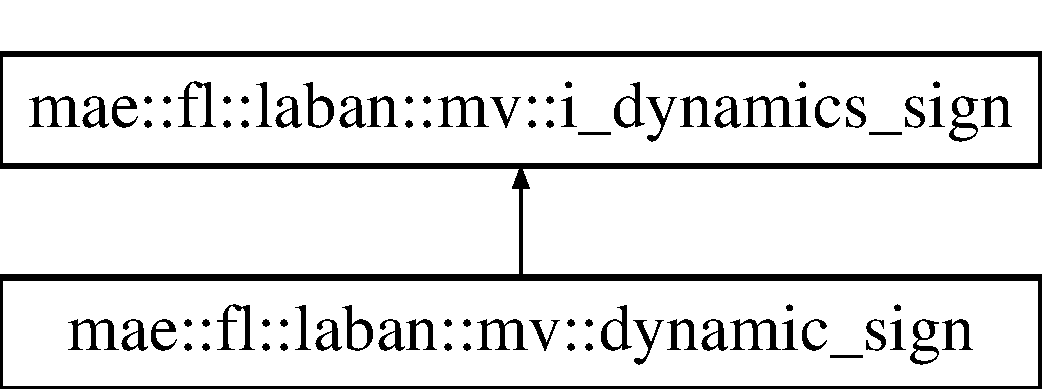
\includegraphics[height=2.000000cm]{classmae_1_1fl_1_1laban_1_1mv_1_1dynamic__sign}
\end{center}
\end{figure}
\subsection*{Public Member Functions}
\begin{DoxyCompactItemize}
\item 
\hyperlink{classmae_1_1fl_1_1laban_1_1mv_1_1dynamic__sign_ace4e63f4994a93461ba0e63ff87d4203}{dynamic\-\_\-sign} (e\-\_\-dynamic dynamic)
\item 
e\-\_\-dynamic \hyperlink{classmae_1_1fl_1_1laban_1_1mv_1_1dynamic__sign_aa71524ed008b40ba76fd163d7f7945c8}{get\-\_\-dynamic} () const 
\item 
virtual bool \hyperlink{classmae_1_1fl_1_1laban_1_1mv_1_1dynamic__sign_ac03195293621fcc14071e30179d0e5d6}{equals} (std\-::shared\-\_\-ptr$<$ \hyperlink{classmae_1_1fl_1_1laban_1_1mv_1_1i__dynamics__sign}{i\-\_\-dynamics\-\_\-sign} $>$ a) const 
\item 
virtual std\-::string \hyperlink{classmae_1_1fl_1_1laban_1_1mv_1_1dynamic__sign_a0709e2b98aaf86cb4b690f61fda62e43}{xml} (unsigned int indent=0, std\-::string namesp=\char`\"{}\char`\"{}) const 
\end{DoxyCompactItemize}


\subsection{Constructor \& Destructor Documentation}
\hypertarget{classmae_1_1fl_1_1laban_1_1mv_1_1dynamic__sign_ace4e63f4994a93461ba0e63ff87d4203}{\index{mae\-::fl\-::laban\-::mv\-::dynamic\-\_\-sign@{mae\-::fl\-::laban\-::mv\-::dynamic\-\_\-sign}!dynamic\-\_\-sign@{dynamic\-\_\-sign}}
\index{dynamic\-\_\-sign@{dynamic\-\_\-sign}!mae::fl::laban::mv::dynamic_sign@{mae\-::fl\-::laban\-::mv\-::dynamic\-\_\-sign}}
\subsubsection[{dynamic\-\_\-sign}]{\setlength{\rightskip}{0pt plus 5cm}mae\-::fl\-::laban\-::mv\-::dynamic\-\_\-sign\-::dynamic\-\_\-sign (
\begin{DoxyParamCaption}
\item[{e\-\_\-dynamic}]{dynamic}
\end{DoxyParamCaption}
)}}\label{classmae_1_1fl_1_1laban_1_1mv_1_1dynamic__sign_ace4e63f4994a93461ba0e63ff87d4203}
Creates a new dynamics sign.


\begin{DoxyParams}{Parameters}
{\em dynamic} & The dynamic type. \\
\hline
\end{DoxyParams}


\subsection{Member Function Documentation}
\hypertarget{classmae_1_1fl_1_1laban_1_1mv_1_1dynamic__sign_ac03195293621fcc14071e30179d0e5d6}{\index{mae\-::fl\-::laban\-::mv\-::dynamic\-\_\-sign@{mae\-::fl\-::laban\-::mv\-::dynamic\-\_\-sign}!equals@{equals}}
\index{equals@{equals}!mae::fl::laban::mv::dynamic_sign@{mae\-::fl\-::laban\-::mv\-::dynamic\-\_\-sign}}
\subsubsection[{equals}]{\setlength{\rightskip}{0pt plus 5cm}bool mae\-::fl\-::laban\-::mv\-::dynamic\-\_\-sign\-::equals (
\begin{DoxyParamCaption}
\item[{std\-::shared\-\_\-ptr$<$ {\bf i\-\_\-dynamics\-\_\-sign} $>$}]{a}
\end{DoxyParamCaption}
) const\hspace{0.3cm}{\ttfamily [virtual]}}}\label{classmae_1_1fl_1_1laban_1_1mv_1_1dynamic__sign_ac03195293621fcc14071e30179d0e5d6}
Returns true if signs are equal.


\begin{DoxyParams}{Parameters}
{\em a} & The sign to be compared to. \\
\hline
\end{DoxyParams}
\begin{DoxyReturn}{Returns}
True if equal. 
\end{DoxyReturn}


Implements \hyperlink{classmae_1_1fl_1_1laban_1_1mv_1_1i__dynamics__sign_a8fe9ea5e7b50976e66172042ae01a6e3}{mae\-::fl\-::laban\-::mv\-::i\-\_\-dynamics\-\_\-sign}.

\hypertarget{classmae_1_1fl_1_1laban_1_1mv_1_1dynamic__sign_aa71524ed008b40ba76fd163d7f7945c8}{\index{mae\-::fl\-::laban\-::mv\-::dynamic\-\_\-sign@{mae\-::fl\-::laban\-::mv\-::dynamic\-\_\-sign}!get\-\_\-dynamic@{get\-\_\-dynamic}}
\index{get\-\_\-dynamic@{get\-\_\-dynamic}!mae::fl::laban::mv::dynamic_sign@{mae\-::fl\-::laban\-::mv\-::dynamic\-\_\-sign}}
\subsubsection[{get\-\_\-dynamic}]{\setlength{\rightskip}{0pt plus 5cm}e\-\_\-dynamic mae\-::fl\-::laban\-::mv\-::dynamic\-\_\-sign\-::get\-\_\-dynamic (
\begin{DoxyParamCaption}
{}
\end{DoxyParamCaption}
) const}}\label{classmae_1_1fl_1_1laban_1_1mv_1_1dynamic__sign_aa71524ed008b40ba76fd163d7f7945c8}
Returns the dynamic type.

\begin{DoxyReturn}{Returns}
The type. 
\end{DoxyReturn}
\hypertarget{classmae_1_1fl_1_1laban_1_1mv_1_1dynamic__sign_a0709e2b98aaf86cb4b690f61fda62e43}{\index{mae\-::fl\-::laban\-::mv\-::dynamic\-\_\-sign@{mae\-::fl\-::laban\-::mv\-::dynamic\-\_\-sign}!xml@{xml}}
\index{xml@{xml}!mae::fl::laban::mv::dynamic_sign@{mae\-::fl\-::laban\-::mv\-::dynamic\-\_\-sign}}
\subsubsection[{xml}]{\setlength{\rightskip}{0pt plus 5cm}std\-::string mae\-::fl\-::laban\-::mv\-::dynamic\-\_\-sign\-::xml (
\begin{DoxyParamCaption}
\item[{unsigned int}]{indent = {\ttfamily 0}, }
\item[{std\-::string}]{namesp = {\ttfamily \char`\"{}\char`\"{}}}
\end{DoxyParamCaption}
) const\hspace{0.3cm}{\ttfamily [virtual]}}}\label{classmae_1_1fl_1_1laban_1_1mv_1_1dynamic__sign_a0709e2b98aaf86cb4b690f61fda62e43}
Returns the X\-M\-L representation for this element.


\begin{DoxyParams}{Parameters}
{\em indent} & The applied indent. \\
\hline
{\em namesp} & The prefixed X\-M\-L namespace.\\
\hline
\end{DoxyParams}
\begin{DoxyReturn}{Returns}
The X\-M\-L string. 
\end{DoxyReturn}


Implements \hyperlink{classmae_1_1fl_1_1laban_1_1mv_1_1i__dynamics__sign_aa6332ee3990c3b59fbe8035aeae84503}{mae\-::fl\-::laban\-::mv\-::i\-\_\-dynamics\-\_\-sign}.



The documentation for this class was generated from the following files\-:\begin{DoxyCompactItemize}
\item 
src/mae/fl/laban/mv/dynamic\-\_\-sign.\-hpp\item 
src/mae/fl/laban/mv/dynamic\-\_\-sign.\-cpp\end{DoxyCompactItemize}

\hypertarget{classmae_1_1fl_1_1laban_1_1ps_1_1e__area__c}{\section{mae\-:\-:fl\-:\-:laban\-:\-:ps\-:\-:e\-\_\-area\-\_\-c Class Reference}
\label{classmae_1_1fl_1_1laban_1_1ps_1_1e__area__c}\index{mae\-::fl\-::laban\-::ps\-::e\-\_\-area\-\_\-c@{mae\-::fl\-::laban\-::ps\-::e\-\_\-area\-\_\-c}}
}
\subsection*{Static Public Member Functions}
\begin{DoxyCompactItemize}
\item 
static std\-::string \hyperlink{classmae_1_1fl_1_1laban_1_1ps_1_1e__area__c_a78ef96fbbc5eaddadf9565fb8ce14af3}{str} (e\-\_\-area area)
\item 
static std\-::vector$<$ e\-\_\-area $>$ \hyperlink{classmae_1_1fl_1_1laban_1_1ps_1_1e__area__c_a9783e18e7b0d247c951165d28f4aa2f8}{vec} ()
\item 
static e\-\_\-area \hyperlink{classmae_1_1fl_1_1laban_1_1ps_1_1e__area__c_a75da5bf4f3081ed40a00dd34c7203cb0}{parse} (std\-::string \hyperlink{classmae_1_1fl_1_1laban_1_1ps_1_1e__area__c_a78ef96fbbc5eaddadf9565fb8ce14af3}{str})
\end{DoxyCompactItemize}


\subsection{Member Function Documentation}
\hypertarget{classmae_1_1fl_1_1laban_1_1ps_1_1e__area__c_a75da5bf4f3081ed40a00dd34c7203cb0}{\index{mae\-::fl\-::laban\-::ps\-::e\-\_\-area\-\_\-c@{mae\-::fl\-::laban\-::ps\-::e\-\_\-area\-\_\-c}!parse@{parse}}
\index{parse@{parse}!mae::fl::laban::ps::e_area_c@{mae\-::fl\-::laban\-::ps\-::e\-\_\-area\-\_\-c}}
\subsubsection[{parse}]{\setlength{\rightskip}{0pt plus 5cm}e\-\_\-area mae\-::fl\-::laban\-::ps\-::e\-\_\-area\-\_\-c\-::parse (
\begin{DoxyParamCaption}
\item[{std\-::string}]{str}
\end{DoxyParamCaption}
)\hspace{0.3cm}{\ttfamily [static]}}}\label{classmae_1_1fl_1_1laban_1_1ps_1_1e__area__c_a75da5bf4f3081ed40a00dd34c7203cb0}
Parses the string and returns the corresponding element.


\begin{DoxyParams}{Parameters}
{\em str} & The string to be parsed. \\
\hline
\end{DoxyParams}
\begin{DoxyReturn}{Returns}
The element. 
\end{DoxyReturn}
\hypertarget{classmae_1_1fl_1_1laban_1_1ps_1_1e__area__c_a78ef96fbbc5eaddadf9565fb8ce14af3}{\index{mae\-::fl\-::laban\-::ps\-::e\-\_\-area\-\_\-c@{mae\-::fl\-::laban\-::ps\-::e\-\_\-area\-\_\-c}!str@{str}}
\index{str@{str}!mae::fl::laban::ps::e_area_c@{mae\-::fl\-::laban\-::ps\-::e\-\_\-area\-\_\-c}}
\subsubsection[{str}]{\setlength{\rightskip}{0pt plus 5cm}std\-::string mae\-::fl\-::laban\-::ps\-::e\-\_\-area\-\_\-c\-::str (
\begin{DoxyParamCaption}
\item[{e\-\_\-area}]{area}
\end{DoxyParamCaption}
)\hspace{0.3cm}{\ttfamily [static]}}}\label{classmae_1_1fl_1_1laban_1_1ps_1_1e__area__c_a78ef96fbbc5eaddadf9565fb8ce14af3}
Returns the string representation for this enum value.


\begin{DoxyParams}{Parameters}
{\em area} & The element. \\
\hline
\end{DoxyParams}
\begin{DoxyReturn}{Returns}
The string representation. 
\end{DoxyReturn}
\hypertarget{classmae_1_1fl_1_1laban_1_1ps_1_1e__area__c_a9783e18e7b0d247c951165d28f4aa2f8}{\index{mae\-::fl\-::laban\-::ps\-::e\-\_\-area\-\_\-c@{mae\-::fl\-::laban\-::ps\-::e\-\_\-area\-\_\-c}!vec@{vec}}
\index{vec@{vec}!mae::fl::laban::ps::e_area_c@{mae\-::fl\-::laban\-::ps\-::e\-\_\-area\-\_\-c}}
\subsubsection[{vec}]{\setlength{\rightskip}{0pt plus 5cm}std\-::vector$<$ e\-\_\-area $>$ mae\-::fl\-::laban\-::ps\-::e\-\_\-area\-\_\-c\-::vec (
\begin{DoxyParamCaption}
{}
\end{DoxyParamCaption}
)\hspace{0.3cm}{\ttfamily [static]}}}\label{classmae_1_1fl_1_1laban_1_1ps_1_1e__area__c_a9783e18e7b0d247c951165d28f4aa2f8}
Returns a vector containing all possible enum values.

\begin{DoxyReturn}{Returns}
A vector. 
\end{DoxyReturn}


The documentation for this class was generated from the following files\-:\begin{DoxyCompactItemize}
\item 
src/mae/fl/laban/ps/e\-\_\-area.\-hpp\item 
src/mae/fl/laban/ps/e\-\_\-area.\-cpp\end{DoxyCompactItemize}

\hypertarget{classmae_1_1e__bone__c}{\section{mae\-:\-:e\-\_\-bone\-\_\-c Class Reference}
\label{classmae_1_1e__bone__c}\index{mae\-::e\-\_\-bone\-\_\-c@{mae\-::e\-\_\-bone\-\_\-c}}
}
\subsection*{Static Public Member Functions}
\begin{DoxyCompactItemize}
\item 
static std\-::string \hyperlink{classmae_1_1e__bone__c_ab6369b5e23fbb23f4942d79ca919e424}{str} (e\-\_\-bone \hyperlink{classmae_1_1bone}{bone})
\item 
static int \hyperlink{classmae_1_1e__bone__c_af2ec456747753ddb0ca009e5c7977e00}{to\-\_\-int} (e\-\_\-bone \hyperlink{classmae_1_1bone}{bone})
\item 
static std\-::vector$<$ e\-\_\-bone $>$ \hyperlink{classmae_1_1e__bone__c_a5192fc3428f19290dfc4e2383c0a391f}{vec} ()
\item 
static e\-\_\-bone \hyperlink{classmae_1_1e__bone__c_ae80c307f32c409e3ab6f2cbd03dcedd2}{parse} (std\-::string \hyperlink{classmae_1_1e__bone__c_ab6369b5e23fbb23f4942d79ca919e424}{str})
\end{DoxyCompactItemize}


\subsection{Member Function Documentation}
\hypertarget{classmae_1_1e__bone__c_ae80c307f32c409e3ab6f2cbd03dcedd2}{\index{mae\-::e\-\_\-bone\-\_\-c@{mae\-::e\-\_\-bone\-\_\-c}!parse@{parse}}
\index{parse@{parse}!mae::e_bone_c@{mae\-::e\-\_\-bone\-\_\-c}}
\subsubsection[{parse}]{\setlength{\rightskip}{0pt plus 5cm}e\-\_\-bone mae\-::e\-\_\-bone\-\_\-c\-::parse (
\begin{DoxyParamCaption}
\item[{std\-::string}]{str}
\end{DoxyParamCaption}
)\hspace{0.3cm}{\ttfamily [static]}}}\label{classmae_1_1e__bone__c_ae80c307f32c409e3ab6f2cbd03dcedd2}
Parses the string and returns the corresponding element.


\begin{DoxyParams}{Parameters}
{\em str} & The string to be parsed. \\
\hline
\end{DoxyParams}
\begin{DoxyReturn}{Returns}
The element. 
\end{DoxyReturn}
\hypertarget{classmae_1_1e__bone__c_ab6369b5e23fbb23f4942d79ca919e424}{\index{mae\-::e\-\_\-bone\-\_\-c@{mae\-::e\-\_\-bone\-\_\-c}!str@{str}}
\index{str@{str}!mae::e_bone_c@{mae\-::e\-\_\-bone\-\_\-c}}
\subsubsection[{str}]{\setlength{\rightskip}{0pt plus 5cm}std\-::string mae\-::e\-\_\-bone\-\_\-c\-::str (
\begin{DoxyParamCaption}
\item[{e\-\_\-bone}]{bone}
\end{DoxyParamCaption}
)\hspace{0.3cm}{\ttfamily [static]}}}\label{classmae_1_1e__bone__c_ab6369b5e23fbb23f4942d79ca919e424}
Returns the string representation for this enum value.


\begin{DoxyParams}{Parameters}
{\em bone} & The element. \\
\hline
\end{DoxyParams}
\begin{DoxyReturn}{Returns}
The string representation. 
\end{DoxyReturn}
\hypertarget{classmae_1_1e__bone__c_af2ec456747753ddb0ca009e5c7977e00}{\index{mae\-::e\-\_\-bone\-\_\-c@{mae\-::e\-\_\-bone\-\_\-c}!to\-\_\-int@{to\-\_\-int}}
\index{to\-\_\-int@{to\-\_\-int}!mae::e_bone_c@{mae\-::e\-\_\-bone\-\_\-c}}
\subsubsection[{to\-\_\-int}]{\setlength{\rightskip}{0pt plus 5cm}int mae\-::e\-\_\-bone\-\_\-c\-::to\-\_\-int (
\begin{DoxyParamCaption}
\item[{e\-\_\-bone}]{bone}
\end{DoxyParamCaption}
)\hspace{0.3cm}{\ttfamily [static]}}}\label{classmae_1_1e__bone__c_af2ec456747753ddb0ca009e5c7977e00}
Returns the integer value corresponding to this element.


\begin{DoxyParams}{Parameters}
{\em bone} & The element. \\
\hline
\end{DoxyParams}
\begin{DoxyReturn}{Returns}
The integer I\-D. 
\end{DoxyReturn}
\hypertarget{classmae_1_1e__bone__c_a5192fc3428f19290dfc4e2383c0a391f}{\index{mae\-::e\-\_\-bone\-\_\-c@{mae\-::e\-\_\-bone\-\_\-c}!vec@{vec}}
\index{vec@{vec}!mae::e_bone_c@{mae\-::e\-\_\-bone\-\_\-c}}
\subsubsection[{vec}]{\setlength{\rightskip}{0pt plus 5cm}std\-::vector$<$ e\-\_\-bone $>$ mae\-::e\-\_\-bone\-\_\-c\-::vec (
\begin{DoxyParamCaption}
{}
\end{DoxyParamCaption}
)\hspace{0.3cm}{\ttfamily [static]}}}\label{classmae_1_1e__bone__c_a5192fc3428f19290dfc4e2383c0a391f}
Returns a vector containing all possible enum values.

\begin{DoxyReturn}{Returns}
A vector. 
\end{DoxyReturn}


The documentation for this class was generated from the following files\-:\begin{DoxyCompactItemize}
\item 
src/mae/e\-\_\-bone.\-hpp\item 
src/mae/e\-\_\-bone.\-cpp\end{DoxyCompactItemize}

\hypertarget{classmae_1_1fl_1_1laban_1_1mv_1_1e__cancel__c}{\section{mae\-:\-:fl\-:\-:laban\-:\-:mv\-:\-:e\-\_\-cancel\-\_\-c Class Reference}
\label{classmae_1_1fl_1_1laban_1_1mv_1_1e__cancel__c}\index{mae\-::fl\-::laban\-::mv\-::e\-\_\-cancel\-\_\-c@{mae\-::fl\-::laban\-::mv\-::e\-\_\-cancel\-\_\-c}}
}
\subsection*{Static Public Member Functions}
\begin{DoxyCompactItemize}
\item 
static std\-::string \hyperlink{classmae_1_1fl_1_1laban_1_1mv_1_1e__cancel__c_a6395b6374f8fdf7100f891a8602b3d91}{str} (e\-\_\-cancel cancel)
\item 
static std\-::vector$<$ e\-\_\-cancel $>$ \hyperlink{classmae_1_1fl_1_1laban_1_1mv_1_1e__cancel__c_a513a39ae91c6e22b9785baf71ba1442d}{vec} ()
\item 
static e\-\_\-cancel \hyperlink{classmae_1_1fl_1_1laban_1_1mv_1_1e__cancel__c_a7afaea57b2b6d9c07700873fd35d51e3}{parse} (std\-::string \hyperlink{classmae_1_1fl_1_1laban_1_1mv_1_1e__cancel__c_a6395b6374f8fdf7100f891a8602b3d91}{str})
\end{DoxyCompactItemize}


\subsection{Member Function Documentation}
\hypertarget{classmae_1_1fl_1_1laban_1_1mv_1_1e__cancel__c_a7afaea57b2b6d9c07700873fd35d51e3}{\index{mae\-::fl\-::laban\-::mv\-::e\-\_\-cancel\-\_\-c@{mae\-::fl\-::laban\-::mv\-::e\-\_\-cancel\-\_\-c}!parse@{parse}}
\index{parse@{parse}!mae::fl::laban::mv::e_cancel_c@{mae\-::fl\-::laban\-::mv\-::e\-\_\-cancel\-\_\-c}}
\subsubsection[{parse}]{\setlength{\rightskip}{0pt plus 5cm}e\-\_\-cancel mae\-::fl\-::laban\-::mv\-::e\-\_\-cancel\-\_\-c\-::parse (
\begin{DoxyParamCaption}
\item[{std\-::string}]{str}
\end{DoxyParamCaption}
)\hspace{0.3cm}{\ttfamily [static]}}}\label{classmae_1_1fl_1_1laban_1_1mv_1_1e__cancel__c_a7afaea57b2b6d9c07700873fd35d51e3}
Parses the string and returns the corresponding element.


\begin{DoxyParams}{Parameters}
{\em str} & The string to be parsed. \\
\hline
\end{DoxyParams}
\begin{DoxyReturn}{Returns}
The element. 
\end{DoxyReturn}
\hypertarget{classmae_1_1fl_1_1laban_1_1mv_1_1e__cancel__c_a6395b6374f8fdf7100f891a8602b3d91}{\index{mae\-::fl\-::laban\-::mv\-::e\-\_\-cancel\-\_\-c@{mae\-::fl\-::laban\-::mv\-::e\-\_\-cancel\-\_\-c}!str@{str}}
\index{str@{str}!mae::fl::laban::mv::e_cancel_c@{mae\-::fl\-::laban\-::mv\-::e\-\_\-cancel\-\_\-c}}
\subsubsection[{str}]{\setlength{\rightskip}{0pt plus 5cm}std\-::string mae\-::fl\-::laban\-::mv\-::e\-\_\-cancel\-\_\-c\-::str (
\begin{DoxyParamCaption}
\item[{e\-\_\-cancel}]{cancel}
\end{DoxyParamCaption}
)\hspace{0.3cm}{\ttfamily [static]}}}\label{classmae_1_1fl_1_1laban_1_1mv_1_1e__cancel__c_a6395b6374f8fdf7100f891a8602b3d91}
Returns the string representation for this enum value.


\begin{DoxyParams}{Parameters}
{\em cancel} & The element. \\
\hline
\end{DoxyParams}
\begin{DoxyReturn}{Returns}
The string representation. 
\end{DoxyReturn}
\hypertarget{classmae_1_1fl_1_1laban_1_1mv_1_1e__cancel__c_a513a39ae91c6e22b9785baf71ba1442d}{\index{mae\-::fl\-::laban\-::mv\-::e\-\_\-cancel\-\_\-c@{mae\-::fl\-::laban\-::mv\-::e\-\_\-cancel\-\_\-c}!vec@{vec}}
\index{vec@{vec}!mae::fl::laban::mv::e_cancel_c@{mae\-::fl\-::laban\-::mv\-::e\-\_\-cancel\-\_\-c}}
\subsubsection[{vec}]{\setlength{\rightskip}{0pt plus 5cm}std\-::vector$<$ e\-\_\-cancel $>$ mae\-::fl\-::laban\-::mv\-::e\-\_\-cancel\-\_\-c\-::vec (
\begin{DoxyParamCaption}
{}
\end{DoxyParamCaption}
)\hspace{0.3cm}{\ttfamily [static]}}}\label{classmae_1_1fl_1_1laban_1_1mv_1_1e__cancel__c_a513a39ae91c6e22b9785baf71ba1442d}
Returns a vector containing all possible enum values.

\begin{DoxyReturn}{Returns}
A vector. 
\end{DoxyReturn}


The documentation for this class was generated from the following files\-:\begin{DoxyCompactItemize}
\item 
src/mae/fl/laban/mv/e\-\_\-cancel.\-hpp\item 
src/mae/fl/laban/mv/e\-\_\-cancel.\-cpp\end{DoxyCompactItemize}

\hypertarget{classmae_1_1fl_1_1laban_1_1mv_1_1e__contact__hook__c}{\section{mae\-:\-:fl\-:\-:laban\-:\-:mv\-:\-:e\-\_\-contact\-\_\-hook\-\_\-c Class Reference}
\label{classmae_1_1fl_1_1laban_1_1mv_1_1e__contact__hook__c}\index{mae\-::fl\-::laban\-::mv\-::e\-\_\-contact\-\_\-hook\-\_\-c@{mae\-::fl\-::laban\-::mv\-::e\-\_\-contact\-\_\-hook\-\_\-c}}
}
\subsection*{Static Public Member Functions}
\begin{DoxyCompactItemize}
\item 
static std\-::string \hyperlink{classmae_1_1fl_1_1laban_1_1mv_1_1e__contact__hook__c_a36b1a65947a5c6732f87193c5c657509}{str} (e\-\_\-contact\-\_\-hook hook)
\item 
static std\-::vector\\*
$<$ e\-\_\-contact\-\_\-hook $>$ \hyperlink{classmae_1_1fl_1_1laban_1_1mv_1_1e__contact__hook__c_ae06626fed82b0a3e0ba4e7072c484733}{vec} ()
\item 
static e\-\_\-contact\-\_\-hook \hyperlink{classmae_1_1fl_1_1laban_1_1mv_1_1e__contact__hook__c_ab15c1b58aec51699252d0080d4efce6e}{parse} (std\-::string \hyperlink{classmae_1_1fl_1_1laban_1_1mv_1_1e__contact__hook__c_a36b1a65947a5c6732f87193c5c657509}{str})
\end{DoxyCompactItemize}


\subsection{Member Function Documentation}
\hypertarget{classmae_1_1fl_1_1laban_1_1mv_1_1e__contact__hook__c_ab15c1b58aec51699252d0080d4efce6e}{\index{mae\-::fl\-::laban\-::mv\-::e\-\_\-contact\-\_\-hook\-\_\-c@{mae\-::fl\-::laban\-::mv\-::e\-\_\-contact\-\_\-hook\-\_\-c}!parse@{parse}}
\index{parse@{parse}!mae::fl::laban::mv::e_contact_hook_c@{mae\-::fl\-::laban\-::mv\-::e\-\_\-contact\-\_\-hook\-\_\-c}}
\subsubsection[{parse}]{\setlength{\rightskip}{0pt plus 5cm}e\-\_\-contact\-\_\-hook mae\-::fl\-::laban\-::mv\-::e\-\_\-contact\-\_\-hook\-\_\-c\-::parse (
\begin{DoxyParamCaption}
\item[{std\-::string}]{str}
\end{DoxyParamCaption}
)\hspace{0.3cm}{\ttfamily [static]}}}\label{classmae_1_1fl_1_1laban_1_1mv_1_1e__contact__hook__c_ab15c1b58aec51699252d0080d4efce6e}
Parses the string and returns the corresponding element.


\begin{DoxyParams}{Parameters}
{\em str} & The string to be parsed. \\
\hline
\end{DoxyParams}
\begin{DoxyReturn}{Returns}
The element. 
\end{DoxyReturn}
\hypertarget{classmae_1_1fl_1_1laban_1_1mv_1_1e__contact__hook__c_a36b1a65947a5c6732f87193c5c657509}{\index{mae\-::fl\-::laban\-::mv\-::e\-\_\-contact\-\_\-hook\-\_\-c@{mae\-::fl\-::laban\-::mv\-::e\-\_\-contact\-\_\-hook\-\_\-c}!str@{str}}
\index{str@{str}!mae::fl::laban::mv::e_contact_hook_c@{mae\-::fl\-::laban\-::mv\-::e\-\_\-contact\-\_\-hook\-\_\-c}}
\subsubsection[{str}]{\setlength{\rightskip}{0pt plus 5cm}std\-::string mae\-::fl\-::laban\-::mv\-::e\-\_\-contact\-\_\-hook\-\_\-c\-::str (
\begin{DoxyParamCaption}
\item[{e\-\_\-contact\-\_\-hook}]{hook}
\end{DoxyParamCaption}
)\hspace{0.3cm}{\ttfamily [static]}}}\label{classmae_1_1fl_1_1laban_1_1mv_1_1e__contact__hook__c_a36b1a65947a5c6732f87193c5c657509}
Returns the string representation for this enum value.


\begin{DoxyParams}{Parameters}
{\em hook} & The element. \\
\hline
\end{DoxyParams}
\begin{DoxyReturn}{Returns}
The string representation. 
\end{DoxyReturn}
\hypertarget{classmae_1_1fl_1_1laban_1_1mv_1_1e__contact__hook__c_ae06626fed82b0a3e0ba4e7072c484733}{\index{mae\-::fl\-::laban\-::mv\-::e\-\_\-contact\-\_\-hook\-\_\-c@{mae\-::fl\-::laban\-::mv\-::e\-\_\-contact\-\_\-hook\-\_\-c}!vec@{vec}}
\index{vec@{vec}!mae::fl::laban::mv::e_contact_hook_c@{mae\-::fl\-::laban\-::mv\-::e\-\_\-contact\-\_\-hook\-\_\-c}}
\subsubsection[{vec}]{\setlength{\rightskip}{0pt plus 5cm}std\-::vector$<$ e\-\_\-contact\-\_\-hook $>$ mae\-::fl\-::laban\-::mv\-::e\-\_\-contact\-\_\-hook\-\_\-c\-::vec (
\begin{DoxyParamCaption}
{}
\end{DoxyParamCaption}
)\hspace{0.3cm}{\ttfamily [static]}}}\label{classmae_1_1fl_1_1laban_1_1mv_1_1e__contact__hook__c_ae06626fed82b0a3e0ba4e7072c484733}
Returns a vector containing all possible enum values.

\begin{DoxyReturn}{Returns}
A vector. 
\end{DoxyReturn}


The documentation for this class was generated from the following files\-:\begin{DoxyCompactItemize}
\item 
src/mae/fl/laban/mv/e\-\_\-contact\-\_\-hook.\-hpp\item 
src/mae/fl/laban/mv/e\-\_\-contact\-\_\-hook.\-cpp\end{DoxyCompactItemize}

\hypertarget{classmae_1_1fl_1_1laban_1_1ps_1_1e__digit__c}{\section{mae\-:\-:fl\-:\-:laban\-:\-:ps\-:\-:e\-\_\-digit\-\_\-c Class Reference}
\label{classmae_1_1fl_1_1laban_1_1ps_1_1e__digit__c}\index{mae\-::fl\-::laban\-::ps\-::e\-\_\-digit\-\_\-c@{mae\-::fl\-::laban\-::ps\-::e\-\_\-digit\-\_\-c}}
}
\subsection*{Static Public Member Functions}
\begin{DoxyCompactItemize}
\item 
static std\-::string \hyperlink{classmae_1_1fl_1_1laban_1_1ps_1_1e__digit__c_ace4c9e7f2bef858c0cd92a2df40d53d9}{str} (e\-\_\-digit digit)
\item 
static std\-::vector$<$ e\-\_\-digit $>$ \hyperlink{classmae_1_1fl_1_1laban_1_1ps_1_1e__digit__c_a4f967d356145815c0231a2707bdd91e6}{vec} ()
\item 
static e\-\_\-digit \hyperlink{classmae_1_1fl_1_1laban_1_1ps_1_1e__digit__c_abb09951e597cf2aeb20fc20c663d2f43}{parse} (std\-::string \hyperlink{classmae_1_1fl_1_1laban_1_1ps_1_1e__digit__c_ace4c9e7f2bef858c0cd92a2df40d53d9}{str})
\end{DoxyCompactItemize}


\subsection{Member Function Documentation}
\hypertarget{classmae_1_1fl_1_1laban_1_1ps_1_1e__digit__c_abb09951e597cf2aeb20fc20c663d2f43}{\index{mae\-::fl\-::laban\-::ps\-::e\-\_\-digit\-\_\-c@{mae\-::fl\-::laban\-::ps\-::e\-\_\-digit\-\_\-c}!parse@{parse}}
\index{parse@{parse}!mae::fl::laban::ps::e_digit_c@{mae\-::fl\-::laban\-::ps\-::e\-\_\-digit\-\_\-c}}
\subsubsection[{parse}]{\setlength{\rightskip}{0pt plus 5cm}e\-\_\-digit mae\-::fl\-::laban\-::ps\-::e\-\_\-digit\-\_\-c\-::parse (
\begin{DoxyParamCaption}
\item[{std\-::string}]{str}
\end{DoxyParamCaption}
)\hspace{0.3cm}{\ttfamily [static]}}}\label{classmae_1_1fl_1_1laban_1_1ps_1_1e__digit__c_abb09951e597cf2aeb20fc20c663d2f43}
Parses the string and returns the corresponding element.


\begin{DoxyParams}{Parameters}
{\em str} & The string to be parsed. \\
\hline
\end{DoxyParams}
\begin{DoxyReturn}{Returns}
The element. 
\end{DoxyReturn}
\hypertarget{classmae_1_1fl_1_1laban_1_1ps_1_1e__digit__c_ace4c9e7f2bef858c0cd92a2df40d53d9}{\index{mae\-::fl\-::laban\-::ps\-::e\-\_\-digit\-\_\-c@{mae\-::fl\-::laban\-::ps\-::e\-\_\-digit\-\_\-c}!str@{str}}
\index{str@{str}!mae::fl::laban::ps::e_digit_c@{mae\-::fl\-::laban\-::ps\-::e\-\_\-digit\-\_\-c}}
\subsubsection[{str}]{\setlength{\rightskip}{0pt plus 5cm}std\-::string mae\-::fl\-::laban\-::ps\-::e\-\_\-digit\-\_\-c\-::str (
\begin{DoxyParamCaption}
\item[{e\-\_\-digit}]{digit}
\end{DoxyParamCaption}
)\hspace{0.3cm}{\ttfamily [static]}}}\label{classmae_1_1fl_1_1laban_1_1ps_1_1e__digit__c_ace4c9e7f2bef858c0cd92a2df40d53d9}
Returns the string representation for this enum value.


\begin{DoxyParams}{Parameters}
{\em digit} & The element. \\
\hline
\end{DoxyParams}
\begin{DoxyReturn}{Returns}
The string representation. 
\end{DoxyReturn}
\hypertarget{classmae_1_1fl_1_1laban_1_1ps_1_1e__digit__c_a4f967d356145815c0231a2707bdd91e6}{\index{mae\-::fl\-::laban\-::ps\-::e\-\_\-digit\-\_\-c@{mae\-::fl\-::laban\-::ps\-::e\-\_\-digit\-\_\-c}!vec@{vec}}
\index{vec@{vec}!mae::fl::laban::ps::e_digit_c@{mae\-::fl\-::laban\-::ps\-::e\-\_\-digit\-\_\-c}}
\subsubsection[{vec}]{\setlength{\rightskip}{0pt plus 5cm}std\-::vector$<$ e\-\_\-digit $>$ mae\-::fl\-::laban\-::ps\-::e\-\_\-digit\-\_\-c\-::vec (
\begin{DoxyParamCaption}
{}
\end{DoxyParamCaption}
)\hspace{0.3cm}{\ttfamily [static]}}}\label{classmae_1_1fl_1_1laban_1_1ps_1_1e__digit__c_a4f967d356145815c0231a2707bdd91e6}
Returns a vector containing all possible enum values.

\begin{DoxyReturn}{Returns}
A vector. 
\end{DoxyReturn}


The documentation for this class was generated from the following files\-:\begin{DoxyCompactItemize}
\item 
src/mae/fl/laban/ps/e\-\_\-digit.\-hpp\item 
src/mae/fl/laban/ps/e\-\_\-digit.\-cpp\end{DoxyCompactItemize}

\hypertarget{classmae_1_1fl_1_1laban_1_1mv_1_1e__direction__c}{\section{mae\-:\-:fl\-:\-:laban\-:\-:mv\-:\-:e\-\_\-direction\-\_\-c Class Reference}
\label{classmae_1_1fl_1_1laban_1_1mv_1_1e__direction__c}\index{mae\-::fl\-::laban\-::mv\-::e\-\_\-direction\-\_\-c@{mae\-::fl\-::laban\-::mv\-::e\-\_\-direction\-\_\-c}}
}
\subsection*{Static Public Member Functions}
\begin{DoxyCompactItemize}
\item 
static std\-::string \hyperlink{classmae_1_1fl_1_1laban_1_1mv_1_1e__direction__c_a96514e42d8eeac4751be72d1f1b5d8d2}{str} (e\-\_\-direction direction)
\item 
static e\-\_\-direction \hyperlink{classmae_1_1fl_1_1laban_1_1mv_1_1e__direction__c_a86ebc4692d9de0074cf4c193b3194c3a}{dir} (e\-\_\-fl\-\_\-direction direction)
\item 
static std\-::vector$<$ e\-\_\-direction $>$ \hyperlink{classmae_1_1fl_1_1laban_1_1mv_1_1e__direction__c_a5a05353c2cb17e9dace8a67d41527b46}{vec} ()
\item 
static e\-\_\-direction \hyperlink{classmae_1_1fl_1_1laban_1_1mv_1_1e__direction__c_a21dcd7b639c1b17bab336e284a631a96}{parse} (std\-::string \hyperlink{classmae_1_1fl_1_1laban_1_1mv_1_1e__direction__c_a96514e42d8eeac4751be72d1f1b5d8d2}{str})
\end{DoxyCompactItemize}


\subsection{Member Function Documentation}
\hypertarget{classmae_1_1fl_1_1laban_1_1mv_1_1e__direction__c_a86ebc4692d9de0074cf4c193b3194c3a}{\index{mae\-::fl\-::laban\-::mv\-::e\-\_\-direction\-\_\-c@{mae\-::fl\-::laban\-::mv\-::e\-\_\-direction\-\_\-c}!dir@{dir}}
\index{dir@{dir}!mae::fl::laban::mv::e_direction_c@{mae\-::fl\-::laban\-::mv\-::e\-\_\-direction\-\_\-c}}
\subsubsection[{dir}]{\setlength{\rightskip}{0pt plus 5cm}e\-\_\-direction mae\-::fl\-::laban\-::mv\-::e\-\_\-direction\-\_\-c\-::dir (
\begin{DoxyParamCaption}
\item[{e\-\_\-fl\-\_\-direction}]{direction}
\end{DoxyParamCaption}
)\hspace{0.3cm}{\ttfamily [static]}}}\label{classmae_1_1fl_1_1laban_1_1mv_1_1e__direction__c_a86ebc4692d9de0074cf4c193b3194c3a}
Returns the corresponding direction value.


\begin{DoxyParams}{Parameters}
{\em direction} & The direction+level enum value. \\
\hline
\end{DoxyParams}
\begin{DoxyReturn}{Returns}
The direction. 
\end{DoxyReturn}
\hypertarget{classmae_1_1fl_1_1laban_1_1mv_1_1e__direction__c_a21dcd7b639c1b17bab336e284a631a96}{\index{mae\-::fl\-::laban\-::mv\-::e\-\_\-direction\-\_\-c@{mae\-::fl\-::laban\-::mv\-::e\-\_\-direction\-\_\-c}!parse@{parse}}
\index{parse@{parse}!mae::fl::laban::mv::e_direction_c@{mae\-::fl\-::laban\-::mv\-::e\-\_\-direction\-\_\-c}}
\subsubsection[{parse}]{\setlength{\rightskip}{0pt plus 5cm}e\-\_\-direction mae\-::fl\-::laban\-::mv\-::e\-\_\-direction\-\_\-c\-::parse (
\begin{DoxyParamCaption}
\item[{std\-::string}]{str}
\end{DoxyParamCaption}
)\hspace{0.3cm}{\ttfamily [static]}}}\label{classmae_1_1fl_1_1laban_1_1mv_1_1e__direction__c_a21dcd7b639c1b17bab336e284a631a96}
Parses the string and returns the corresponding element.


\begin{DoxyParams}{Parameters}
{\em str} & The string to be parsed. \\
\hline
\end{DoxyParams}
\begin{DoxyReturn}{Returns}
The element. 
\end{DoxyReturn}
\hypertarget{classmae_1_1fl_1_1laban_1_1mv_1_1e__direction__c_a96514e42d8eeac4751be72d1f1b5d8d2}{\index{mae\-::fl\-::laban\-::mv\-::e\-\_\-direction\-\_\-c@{mae\-::fl\-::laban\-::mv\-::e\-\_\-direction\-\_\-c}!str@{str}}
\index{str@{str}!mae::fl::laban::mv::e_direction_c@{mae\-::fl\-::laban\-::mv\-::e\-\_\-direction\-\_\-c}}
\subsubsection[{str}]{\setlength{\rightskip}{0pt plus 5cm}std\-::string mae\-::fl\-::laban\-::mv\-::e\-\_\-direction\-\_\-c\-::str (
\begin{DoxyParamCaption}
\item[{e\-\_\-direction}]{direction}
\end{DoxyParamCaption}
)\hspace{0.3cm}{\ttfamily [static]}}}\label{classmae_1_1fl_1_1laban_1_1mv_1_1e__direction__c_a96514e42d8eeac4751be72d1f1b5d8d2}
Returns the string representation for this enum value.


\begin{DoxyParams}{Parameters}
{\em direction} & The element. \\
\hline
\end{DoxyParams}
\begin{DoxyReturn}{Returns}
The string representation. 
\end{DoxyReturn}
\hypertarget{classmae_1_1fl_1_1laban_1_1mv_1_1e__direction__c_a5a05353c2cb17e9dace8a67d41527b46}{\index{mae\-::fl\-::laban\-::mv\-::e\-\_\-direction\-\_\-c@{mae\-::fl\-::laban\-::mv\-::e\-\_\-direction\-\_\-c}!vec@{vec}}
\index{vec@{vec}!mae::fl::laban::mv::e_direction_c@{mae\-::fl\-::laban\-::mv\-::e\-\_\-direction\-\_\-c}}
\subsubsection[{vec}]{\setlength{\rightskip}{0pt plus 5cm}std\-::vector$<$ e\-\_\-direction $>$ mae\-::fl\-::laban\-::mv\-::e\-\_\-direction\-\_\-c\-::vec (
\begin{DoxyParamCaption}
{}
\end{DoxyParamCaption}
)\hspace{0.3cm}{\ttfamily [static]}}}\label{classmae_1_1fl_1_1laban_1_1mv_1_1e__direction__c_a5a05353c2cb17e9dace8a67d41527b46}
Returns a vector containing all possible enum values.

\begin{DoxyReturn}{Returns}
A vector. 
\end{DoxyReturn}


The documentation for this class was generated from the following files\-:\begin{DoxyCompactItemize}
\item 
src/mae/fl/laban/mv/e\-\_\-direction.\-hpp\item 
src/mae/fl/laban/mv/e\-\_\-direction.\-cpp\end{DoxyCompactItemize}

\hypertarget{classmae_1_1fl_1_1laban_1_1mv_1_1e__dynamic__c}{\section{mae\-:\-:fl\-:\-:laban\-:\-:mv\-:\-:e\-\_\-dynamic\-\_\-c Class Reference}
\label{classmae_1_1fl_1_1laban_1_1mv_1_1e__dynamic__c}\index{mae\-::fl\-::laban\-::mv\-::e\-\_\-dynamic\-\_\-c@{mae\-::fl\-::laban\-::mv\-::e\-\_\-dynamic\-\_\-c}}
}
\subsection*{Static Public Member Functions}
\begin{DoxyCompactItemize}
\item 
static std\-::string \hyperlink{classmae_1_1fl_1_1laban_1_1mv_1_1e__dynamic__c_aba336ab3c70f97bb8e8f094b982523bc}{str} (e\-\_\-dynamic dynamic)
\item 
static std\-::vector$<$ e\-\_\-dynamic $>$ \hyperlink{classmae_1_1fl_1_1laban_1_1mv_1_1e__dynamic__c_a58cdfa9e52b0d77b500edaa8229ec8b1}{vec} ()
\item 
static e\-\_\-dynamic \hyperlink{classmae_1_1fl_1_1laban_1_1mv_1_1e__dynamic__c_a95065320ed19c021902436a03e987abc}{parse} (std\-::string \hyperlink{classmae_1_1fl_1_1laban_1_1mv_1_1e__dynamic__c_aba336ab3c70f97bb8e8f094b982523bc}{str})
\end{DoxyCompactItemize}


\subsection{Member Function Documentation}
\hypertarget{classmae_1_1fl_1_1laban_1_1mv_1_1e__dynamic__c_a95065320ed19c021902436a03e987abc}{\index{mae\-::fl\-::laban\-::mv\-::e\-\_\-dynamic\-\_\-c@{mae\-::fl\-::laban\-::mv\-::e\-\_\-dynamic\-\_\-c}!parse@{parse}}
\index{parse@{parse}!mae::fl::laban::mv::e_dynamic_c@{mae\-::fl\-::laban\-::mv\-::e\-\_\-dynamic\-\_\-c}}
\subsubsection[{parse}]{\setlength{\rightskip}{0pt plus 5cm}e\-\_\-dynamic mae\-::fl\-::laban\-::mv\-::e\-\_\-dynamic\-\_\-c\-::parse (
\begin{DoxyParamCaption}
\item[{std\-::string}]{str}
\end{DoxyParamCaption}
)\hspace{0.3cm}{\ttfamily [static]}}}\label{classmae_1_1fl_1_1laban_1_1mv_1_1e__dynamic__c_a95065320ed19c021902436a03e987abc}
Parses the string and returns the corresponding element.


\begin{DoxyParams}{Parameters}
{\em str} & The string to be parsed. \\
\hline
\end{DoxyParams}
\begin{DoxyReturn}{Returns}
The element. 
\end{DoxyReturn}
\hypertarget{classmae_1_1fl_1_1laban_1_1mv_1_1e__dynamic__c_aba336ab3c70f97bb8e8f094b982523bc}{\index{mae\-::fl\-::laban\-::mv\-::e\-\_\-dynamic\-\_\-c@{mae\-::fl\-::laban\-::mv\-::e\-\_\-dynamic\-\_\-c}!str@{str}}
\index{str@{str}!mae::fl::laban::mv::e_dynamic_c@{mae\-::fl\-::laban\-::mv\-::e\-\_\-dynamic\-\_\-c}}
\subsubsection[{str}]{\setlength{\rightskip}{0pt plus 5cm}std\-::string mae\-::fl\-::laban\-::mv\-::e\-\_\-dynamic\-\_\-c\-::str (
\begin{DoxyParamCaption}
\item[{e\-\_\-dynamic}]{dynamic}
\end{DoxyParamCaption}
)\hspace{0.3cm}{\ttfamily [static]}}}\label{classmae_1_1fl_1_1laban_1_1mv_1_1e__dynamic__c_aba336ab3c70f97bb8e8f094b982523bc}
Returns the string representation for this enum value.


\begin{DoxyParams}{Parameters}
{\em dynamic} & The element. \\
\hline
\end{DoxyParams}
\begin{DoxyReturn}{Returns}
The string representation. 
\end{DoxyReturn}
\hypertarget{classmae_1_1fl_1_1laban_1_1mv_1_1e__dynamic__c_a58cdfa9e52b0d77b500edaa8229ec8b1}{\index{mae\-::fl\-::laban\-::mv\-::e\-\_\-dynamic\-\_\-c@{mae\-::fl\-::laban\-::mv\-::e\-\_\-dynamic\-\_\-c}!vec@{vec}}
\index{vec@{vec}!mae::fl::laban::mv::e_dynamic_c@{mae\-::fl\-::laban\-::mv\-::e\-\_\-dynamic\-\_\-c}}
\subsubsection[{vec}]{\setlength{\rightskip}{0pt plus 5cm}std\-::vector$<$ e\-\_\-dynamic $>$ mae\-::fl\-::laban\-::mv\-::e\-\_\-dynamic\-\_\-c\-::vec (
\begin{DoxyParamCaption}
{}
\end{DoxyParamCaption}
)\hspace{0.3cm}{\ttfamily [static]}}}\label{classmae_1_1fl_1_1laban_1_1mv_1_1e__dynamic__c_a58cdfa9e52b0d77b500edaa8229ec8b1}
Returns a vector containing all possible enum values.

\begin{DoxyReturn}{Returns}
A vector. 
\end{DoxyReturn}


The documentation for this class was generated from the following files\-:\begin{DoxyCompactItemize}
\item 
src/mae/fl/laban/mv/e\-\_\-dynamic.\-hpp\item 
src/mae/fl/laban/mv/e\-\_\-dynamic.\-cpp\end{DoxyCompactItemize}

\hypertarget{classmae_1_1fl_1_1e__fl__direction__c}{\section{mae\-:\-:fl\-:\-:e\-\_\-fl\-\_\-direction\-\_\-c Class Reference}
\label{classmae_1_1fl_1_1e__fl__direction__c}\index{mae\-::fl\-::e\-\_\-fl\-\_\-direction\-\_\-c@{mae\-::fl\-::e\-\_\-fl\-\_\-direction\-\_\-c}}
}
\subsection*{Static Public Member Functions}
\begin{DoxyCompactItemize}
\item 
static std\-::string \hyperlink{classmae_1_1fl_1_1e__fl__direction__c_aa5bc4fd04b20f9702f1c7ddfb2263bdb}{str} (e\-\_\-fl\-\_\-direction direction)
\item 
static int \hyperlink{classmae_1_1fl_1_1e__fl__direction__c_a493625ab3f77cb83bc05c1fb96d65cbb}{to\-\_\-int} (e\-\_\-fl\-\_\-direction direction)
\item 
static e\-\_\-fl\-\_\-direction \hyperlink{classmae_1_1fl_1_1e__fl__direction__c_a1ff522cccd852e96e9b8abdb1624ed28}{dir} (laban\-::mv\-::e\-\_\-direction direction, laban\-::mv\-::e\-\_\-level level, bool left=true)
\item 
static std\-::vector\\*
$<$ e\-\_\-fl\-\_\-direction $>$ \hyperlink{classmae_1_1fl_1_1e__fl__direction__c_a97e268f5943fbec594b4dc7f5daa5a71}{vec} ()
\item 
static e\-\_\-fl\-\_\-direction \hyperlink{classmae_1_1fl_1_1e__fl__direction__c_a884249750d84ca4ae935f71d8c44de18}{parse} (std\-::string \hyperlink{classmae_1_1fl_1_1e__fl__direction__c_aa5bc4fd04b20f9702f1c7ddfb2263bdb}{str})
\end{DoxyCompactItemize}


\subsection{Member Function Documentation}
\hypertarget{classmae_1_1fl_1_1e__fl__direction__c_a1ff522cccd852e96e9b8abdb1624ed28}{\index{mae\-::fl\-::e\-\_\-fl\-\_\-direction\-\_\-c@{mae\-::fl\-::e\-\_\-fl\-\_\-direction\-\_\-c}!dir@{dir}}
\index{dir@{dir}!mae::fl::e_fl_direction_c@{mae\-::fl\-::e\-\_\-fl\-\_\-direction\-\_\-c}}
\subsubsection[{dir}]{\setlength{\rightskip}{0pt plus 5cm}e\-\_\-fl\-\_\-direction mae\-::fl\-::e\-\_\-fl\-\_\-direction\-\_\-c\-::dir (
\begin{DoxyParamCaption}
\item[{laban\-::mv\-::e\-\_\-direction}]{direction, }
\item[{laban\-::mv\-::e\-\_\-level}]{level, }
\item[{bool}]{left = {\ttfamily true}}
\end{DoxyParamCaption}
)\hspace{0.3cm}{\ttfamily [static]}}}\label{classmae_1_1fl_1_1e__fl__direction__c_a1ff522cccd852e96e9b8abdb1624ed28}
Returns the corresponding direction value.


\begin{DoxyParams}{Parameters}
{\em direction} & The laban direction enum value. \\
\hline
{\em level} & The laban level enum value. \\
\hline
{\em left} & Refers to the side of the body part. True for left side, false for right side. \\
\hline
\end{DoxyParams}
\begin{DoxyReturn}{Returns}
The direction. 
\end{DoxyReturn}
\hypertarget{classmae_1_1fl_1_1e__fl__direction__c_a884249750d84ca4ae935f71d8c44de18}{\index{mae\-::fl\-::e\-\_\-fl\-\_\-direction\-\_\-c@{mae\-::fl\-::e\-\_\-fl\-\_\-direction\-\_\-c}!parse@{parse}}
\index{parse@{parse}!mae::fl::e_fl_direction_c@{mae\-::fl\-::e\-\_\-fl\-\_\-direction\-\_\-c}}
\subsubsection[{parse}]{\setlength{\rightskip}{0pt plus 5cm}e\-\_\-fl\-\_\-direction mae\-::fl\-::e\-\_\-fl\-\_\-direction\-\_\-c\-::parse (
\begin{DoxyParamCaption}
\item[{std\-::string}]{str}
\end{DoxyParamCaption}
)\hspace{0.3cm}{\ttfamily [static]}}}\label{classmae_1_1fl_1_1e__fl__direction__c_a884249750d84ca4ae935f71d8c44de18}
Parses the string and returns the corresponding element.


\begin{DoxyParams}{Parameters}
{\em str} & The string to be parsed. \\
\hline
\end{DoxyParams}
\begin{DoxyReturn}{Returns}
The element. 
\end{DoxyReturn}
\hypertarget{classmae_1_1fl_1_1e__fl__direction__c_aa5bc4fd04b20f9702f1c7ddfb2263bdb}{\index{mae\-::fl\-::e\-\_\-fl\-\_\-direction\-\_\-c@{mae\-::fl\-::e\-\_\-fl\-\_\-direction\-\_\-c}!str@{str}}
\index{str@{str}!mae::fl::e_fl_direction_c@{mae\-::fl\-::e\-\_\-fl\-\_\-direction\-\_\-c}}
\subsubsection[{str}]{\setlength{\rightskip}{0pt plus 5cm}std\-::string mae\-::fl\-::e\-\_\-fl\-\_\-direction\-\_\-c\-::str (
\begin{DoxyParamCaption}
\item[{e\-\_\-fl\-\_\-direction}]{direction}
\end{DoxyParamCaption}
)\hspace{0.3cm}{\ttfamily [static]}}}\label{classmae_1_1fl_1_1e__fl__direction__c_aa5bc4fd04b20f9702f1c7ddfb2263bdb}
Returns the string representation for this enum value.


\begin{DoxyParams}{Parameters}
{\em direction} & The element. \\
\hline
\end{DoxyParams}
\begin{DoxyReturn}{Returns}
The string representation. 
\end{DoxyReturn}
\hypertarget{classmae_1_1fl_1_1e__fl__direction__c_a493625ab3f77cb83bc05c1fb96d65cbb}{\index{mae\-::fl\-::e\-\_\-fl\-\_\-direction\-\_\-c@{mae\-::fl\-::e\-\_\-fl\-\_\-direction\-\_\-c}!to\-\_\-int@{to\-\_\-int}}
\index{to\-\_\-int@{to\-\_\-int}!mae::fl::e_fl_direction_c@{mae\-::fl\-::e\-\_\-fl\-\_\-direction\-\_\-c}}
\subsubsection[{to\-\_\-int}]{\setlength{\rightskip}{0pt plus 5cm}int mae\-::fl\-::e\-\_\-fl\-\_\-direction\-\_\-c\-::to\-\_\-int (
\begin{DoxyParamCaption}
\item[{e\-\_\-fl\-\_\-direction}]{direction}
\end{DoxyParamCaption}
)\hspace{0.3cm}{\ttfamily [static]}}}\label{classmae_1_1fl_1_1e__fl__direction__c_a493625ab3f77cb83bc05c1fb96d65cbb}
Returns the integer value corresponding to this element.


\begin{DoxyParams}{Parameters}
{\em direction} & The element. \\
\hline
\end{DoxyParams}
\begin{DoxyReturn}{Returns}
The integer I\-D. 
\end{DoxyReturn}
\hypertarget{classmae_1_1fl_1_1e__fl__direction__c_a97e268f5943fbec594b4dc7f5daa5a71}{\index{mae\-::fl\-::e\-\_\-fl\-\_\-direction\-\_\-c@{mae\-::fl\-::e\-\_\-fl\-\_\-direction\-\_\-c}!vec@{vec}}
\index{vec@{vec}!mae::fl::e_fl_direction_c@{mae\-::fl\-::e\-\_\-fl\-\_\-direction\-\_\-c}}
\subsubsection[{vec}]{\setlength{\rightskip}{0pt plus 5cm}std\-::vector$<$ e\-\_\-fl\-\_\-direction $>$ mae\-::fl\-::e\-\_\-fl\-\_\-direction\-\_\-c\-::vec (
\begin{DoxyParamCaption}
{}
\end{DoxyParamCaption}
)\hspace{0.3cm}{\ttfamily [static]}}}\label{classmae_1_1fl_1_1e__fl__direction__c_a97e268f5943fbec594b4dc7f5daa5a71}
Returns a vector containing all possible enum values.

\begin{DoxyReturn}{Returns}
A vector. 
\end{DoxyReturn}


The documentation for this class was generated from the following files\-:\begin{DoxyCompactItemize}
\item 
src/mae/fl/e\-\_\-fl\-\_\-direction.\-hpp\item 
src/mae/fl/e\-\_\-fl\-\_\-direction.\-cpp\end{DoxyCompactItemize}

\hypertarget{classmae_1_1fl_1_1e__fl__joint__c}{\section{mae\-:\-:fl\-:\-:e\-\_\-fl\-\_\-joint\-\_\-c Class Reference}
\label{classmae_1_1fl_1_1e__fl__joint__c}\index{mae\-::fl\-::e\-\_\-fl\-\_\-joint\-\_\-c@{mae\-::fl\-::e\-\_\-fl\-\_\-joint\-\_\-c}}
}
\subsection*{Static Public Member Functions}
\begin{DoxyCompactItemize}
\item 
static std\-::string \hyperlink{classmae_1_1fl_1_1e__fl__joint__c_a0e730729332173b7209336685629977b}{str} (e\-\_\-fl\-\_\-joint joint)
\item 
static int \hyperlink{classmae_1_1fl_1_1e__fl__joint__c_a9a2a63fcb99e1d5dc6bd943a0b788635}{to\-\_\-int} (e\-\_\-fl\-\_\-joint joint)
\item 
static std\-::vector$<$ e\-\_\-fl\-\_\-joint $>$ \hyperlink{classmae_1_1fl_1_1e__fl__joint__c_abc77e7531f3dff9b0fbafd265862203d}{vec} ()
\item 
static e\-\_\-fl\-\_\-joint \hyperlink{classmae_1_1fl_1_1e__fl__joint__c_ab21a482e5ea061213510a3b0f4b61126}{parse} (std\-::string \hyperlink{classmae_1_1fl_1_1e__fl__joint__c_a0e730729332173b7209336685629977b}{str})
\end{DoxyCompactItemize}


\subsection{Member Function Documentation}
\hypertarget{classmae_1_1fl_1_1e__fl__joint__c_ab21a482e5ea061213510a3b0f4b61126}{\index{mae\-::fl\-::e\-\_\-fl\-\_\-joint\-\_\-c@{mae\-::fl\-::e\-\_\-fl\-\_\-joint\-\_\-c}!parse@{parse}}
\index{parse@{parse}!mae::fl::e_fl_joint_c@{mae\-::fl\-::e\-\_\-fl\-\_\-joint\-\_\-c}}
\subsubsection[{parse}]{\setlength{\rightskip}{0pt plus 5cm}e\-\_\-fl\-\_\-joint mae\-::fl\-::e\-\_\-fl\-\_\-joint\-\_\-c\-::parse (
\begin{DoxyParamCaption}
\item[{std\-::string}]{str}
\end{DoxyParamCaption}
)\hspace{0.3cm}{\ttfamily [static]}}}\label{classmae_1_1fl_1_1e__fl__joint__c_ab21a482e5ea061213510a3b0f4b61126}
Parses the string and returns the corresponding element.


\begin{DoxyParams}{Parameters}
{\em str} & The string to be parsed. \\
\hline
\end{DoxyParams}
\begin{DoxyReturn}{Returns}
The element. 
\end{DoxyReturn}
\hypertarget{classmae_1_1fl_1_1e__fl__joint__c_a0e730729332173b7209336685629977b}{\index{mae\-::fl\-::e\-\_\-fl\-\_\-joint\-\_\-c@{mae\-::fl\-::e\-\_\-fl\-\_\-joint\-\_\-c}!str@{str}}
\index{str@{str}!mae::fl::e_fl_joint_c@{mae\-::fl\-::e\-\_\-fl\-\_\-joint\-\_\-c}}
\subsubsection[{str}]{\setlength{\rightskip}{0pt plus 5cm}std\-::string mae\-::fl\-::e\-\_\-fl\-\_\-joint\-\_\-c\-::str (
\begin{DoxyParamCaption}
\item[{e\-\_\-fl\-\_\-joint}]{joint}
\end{DoxyParamCaption}
)\hspace{0.3cm}{\ttfamily [static]}}}\label{classmae_1_1fl_1_1e__fl__joint__c_a0e730729332173b7209336685629977b}
Returns the string representation for this enum value.


\begin{DoxyParams}{Parameters}
{\em joint} & The element. \\
\hline
\end{DoxyParams}
\begin{DoxyReturn}{Returns}
The string representation. 
\end{DoxyReturn}
\hypertarget{classmae_1_1fl_1_1e__fl__joint__c_a9a2a63fcb99e1d5dc6bd943a0b788635}{\index{mae\-::fl\-::e\-\_\-fl\-\_\-joint\-\_\-c@{mae\-::fl\-::e\-\_\-fl\-\_\-joint\-\_\-c}!to\-\_\-int@{to\-\_\-int}}
\index{to\-\_\-int@{to\-\_\-int}!mae::fl::e_fl_joint_c@{mae\-::fl\-::e\-\_\-fl\-\_\-joint\-\_\-c}}
\subsubsection[{to\-\_\-int}]{\setlength{\rightskip}{0pt plus 5cm}int mae\-::fl\-::e\-\_\-fl\-\_\-joint\-\_\-c\-::to\-\_\-int (
\begin{DoxyParamCaption}
\item[{e\-\_\-fl\-\_\-joint}]{joint}
\end{DoxyParamCaption}
)\hspace{0.3cm}{\ttfamily [static]}}}\label{classmae_1_1fl_1_1e__fl__joint__c_a9a2a63fcb99e1d5dc6bd943a0b788635}
Returns the integer value corresponding to this element.


\begin{DoxyParams}{Parameters}
{\em joint} & The element. \\
\hline
\end{DoxyParams}
\begin{DoxyReturn}{Returns}
The integer I\-D. 
\end{DoxyReturn}
\hypertarget{classmae_1_1fl_1_1e__fl__joint__c_abc77e7531f3dff9b0fbafd265862203d}{\index{mae\-::fl\-::e\-\_\-fl\-\_\-joint\-\_\-c@{mae\-::fl\-::e\-\_\-fl\-\_\-joint\-\_\-c}!vec@{vec}}
\index{vec@{vec}!mae::fl::e_fl_joint_c@{mae\-::fl\-::e\-\_\-fl\-\_\-joint\-\_\-c}}
\subsubsection[{vec}]{\setlength{\rightskip}{0pt plus 5cm}std\-::vector$<$ e\-\_\-fl\-\_\-joint $>$ mae\-::fl\-::e\-\_\-fl\-\_\-joint\-\_\-c\-::vec (
\begin{DoxyParamCaption}
{}
\end{DoxyParamCaption}
)\hspace{0.3cm}{\ttfamily [static]}}}\label{classmae_1_1fl_1_1e__fl__joint__c_abc77e7531f3dff9b0fbafd265862203d}
Returns a vector containing all possible enum values.

\begin{DoxyReturn}{Returns}
A vector. 
\end{DoxyReturn}


The documentation for this class was generated from the following files\-:\begin{DoxyCompactItemize}
\item 
src/mae/fl/e\-\_\-fl\-\_\-joint.\-hpp\item 
src/mae/fl/e\-\_\-fl\-\_\-joint.\-cpp\end{DoxyCompactItemize}

\hypertarget{classmae_1_1e__joint__c}{\section{mae\-:\-:e\-\_\-joint\-\_\-c Class Reference}
\label{classmae_1_1e__joint__c}\index{mae\-::e\-\_\-joint\-\_\-c@{mae\-::e\-\_\-joint\-\_\-c}}
}
\subsection*{Static Public Member Functions}
\begin{DoxyCompactItemize}
\item 
static std\-::string \hyperlink{classmae_1_1e__joint__c_a5459bfb8c4fd302559098cdc8c86209e}{str} (e\-\_\-joint joint)
\item 
static int \hyperlink{classmae_1_1e__joint__c_a33fd114c946a76fafdf9211a612c259c}{to\-\_\-int} (e\-\_\-joint joint)
\item 
static std\-::vector$<$ e\-\_\-joint $>$ \hyperlink{classmae_1_1e__joint__c_aa97b210e7efa04ad511e2ea115ea77be}{vec} ()
\item 
static bool \hyperlink{classmae_1_1e__joint__c_a7a852d10154adf6830c15663fe91ce5b}{is\-\_\-dummy} (e\-\_\-joint joint)
\item 
static bool \hyperlink{classmae_1_1e__joint__c_a37c7d50beeee004a64db61bacd951385}{is\-\_\-torso} (e\-\_\-joint joint)
\item 
static e\-\_\-joint \hyperlink{classmae_1_1e__joint__c_ac97cd0354b9c75f510c090c080e664e3}{parse} (std\-::string \hyperlink{classmae_1_1e__joint__c_a5459bfb8c4fd302559098cdc8c86209e}{str})
\end{DoxyCompactItemize}


\subsection{Member Function Documentation}
\hypertarget{classmae_1_1e__joint__c_a7a852d10154adf6830c15663fe91ce5b}{\index{mae\-::e\-\_\-joint\-\_\-c@{mae\-::e\-\_\-joint\-\_\-c}!is\-\_\-dummy@{is\-\_\-dummy}}
\index{is\-\_\-dummy@{is\-\_\-dummy}!mae::e_joint_c@{mae\-::e\-\_\-joint\-\_\-c}}
\subsubsection[{is\-\_\-dummy}]{\setlength{\rightskip}{0pt plus 5cm}bool mae\-::e\-\_\-joint\-\_\-c\-::is\-\_\-dummy (
\begin{DoxyParamCaption}
\item[{e\-\_\-joint}]{joint}
\end{DoxyParamCaption}
)\hspace{0.3cm}{\ttfamily [static]}}}\label{classmae_1_1e__joint__c_a7a852d10154adf6830c15663fe91ce5b}
Returns true if the joint I\-D represents a dummy joint.


\begin{DoxyParams}{Parameters}
{\em joint} & The element. \\
\hline
\end{DoxyParams}
\begin{DoxyReturn}{Returns}
True if dummy element. 
\end{DoxyReturn}
\hypertarget{classmae_1_1e__joint__c_a37c7d50beeee004a64db61bacd951385}{\index{mae\-::e\-\_\-joint\-\_\-c@{mae\-::e\-\_\-joint\-\_\-c}!is\-\_\-torso@{is\-\_\-torso}}
\index{is\-\_\-torso@{is\-\_\-torso}!mae::e_joint_c@{mae\-::e\-\_\-joint\-\_\-c}}
\subsubsection[{is\-\_\-torso}]{\setlength{\rightskip}{0pt plus 5cm}bool mae\-::e\-\_\-joint\-\_\-c\-::is\-\_\-torso (
\begin{DoxyParamCaption}
\item[{e\-\_\-joint}]{joint}
\end{DoxyParamCaption}
)\hspace{0.3cm}{\ttfamily [static]}}}\label{classmae_1_1e__joint__c_a37c7d50beeee004a64db61bacd951385}
Returns true if the joint I\-D represents a torso joint.


\begin{DoxyParams}{Parameters}
{\em joint} & The element. \\
\hline
\end{DoxyParams}
\begin{DoxyReturn}{Returns}
True if torso element. 
\end{DoxyReturn}
\hypertarget{classmae_1_1e__joint__c_ac97cd0354b9c75f510c090c080e664e3}{\index{mae\-::e\-\_\-joint\-\_\-c@{mae\-::e\-\_\-joint\-\_\-c}!parse@{parse}}
\index{parse@{parse}!mae::e_joint_c@{mae\-::e\-\_\-joint\-\_\-c}}
\subsubsection[{parse}]{\setlength{\rightskip}{0pt plus 5cm}e\-\_\-joint mae\-::e\-\_\-joint\-\_\-c\-::parse (
\begin{DoxyParamCaption}
\item[{std\-::string}]{str}
\end{DoxyParamCaption}
)\hspace{0.3cm}{\ttfamily [static]}}}\label{classmae_1_1e__joint__c_ac97cd0354b9c75f510c090c080e664e3}
Parses the string and returns the corresponding element.


\begin{DoxyParams}{Parameters}
{\em str} & The string to be parsed. \\
\hline
\end{DoxyParams}
\begin{DoxyReturn}{Returns}
The element. 
\end{DoxyReturn}
\hypertarget{classmae_1_1e__joint__c_a5459bfb8c4fd302559098cdc8c86209e}{\index{mae\-::e\-\_\-joint\-\_\-c@{mae\-::e\-\_\-joint\-\_\-c}!str@{str}}
\index{str@{str}!mae::e_joint_c@{mae\-::e\-\_\-joint\-\_\-c}}
\subsubsection[{str}]{\setlength{\rightskip}{0pt plus 5cm}std\-::string mae\-::e\-\_\-joint\-\_\-c\-::str (
\begin{DoxyParamCaption}
\item[{e\-\_\-joint}]{joint}
\end{DoxyParamCaption}
)\hspace{0.3cm}{\ttfamily [static]}}}\label{classmae_1_1e__joint__c_a5459bfb8c4fd302559098cdc8c86209e}
Returns the string representation for this enum value.


\begin{DoxyParams}{Parameters}
{\em unit} & The element. \\
\hline
\end{DoxyParams}
\begin{DoxyReturn}{Returns}
The string representation. 
\end{DoxyReturn}
\hypertarget{classmae_1_1e__joint__c_a33fd114c946a76fafdf9211a612c259c}{\index{mae\-::e\-\_\-joint\-\_\-c@{mae\-::e\-\_\-joint\-\_\-c}!to\-\_\-int@{to\-\_\-int}}
\index{to\-\_\-int@{to\-\_\-int}!mae::e_joint_c@{mae\-::e\-\_\-joint\-\_\-c}}
\subsubsection[{to\-\_\-int}]{\setlength{\rightskip}{0pt plus 5cm}int mae\-::e\-\_\-joint\-\_\-c\-::to\-\_\-int (
\begin{DoxyParamCaption}
\item[{e\-\_\-joint}]{joint}
\end{DoxyParamCaption}
)\hspace{0.3cm}{\ttfamily [static]}}}\label{classmae_1_1e__joint__c_a33fd114c946a76fafdf9211a612c259c}
Returns the integer value corresponding to this element.


\begin{DoxyParams}{Parameters}
{\em joint} & The element. \\
\hline
\end{DoxyParams}
\begin{DoxyReturn}{Returns}
The integer I\-D. 
\end{DoxyReturn}
\hypertarget{classmae_1_1e__joint__c_aa97b210e7efa04ad511e2ea115ea77be}{\index{mae\-::e\-\_\-joint\-\_\-c@{mae\-::e\-\_\-joint\-\_\-c}!vec@{vec}}
\index{vec@{vec}!mae::e_joint_c@{mae\-::e\-\_\-joint\-\_\-c}}
\subsubsection[{vec}]{\setlength{\rightskip}{0pt plus 5cm}std\-::vector$<$ e\-\_\-joint $>$ mae\-::e\-\_\-joint\-\_\-c\-::vec (
\begin{DoxyParamCaption}
{}
\end{DoxyParamCaption}
)\hspace{0.3cm}{\ttfamily [static]}}}\label{classmae_1_1e__joint__c_aa97b210e7efa04ad511e2ea115ea77be}
Returns a vector containing all possible enum values.

\begin{DoxyReturn}{Returns}
A vector. 
\end{DoxyReturn}


The documentation for this class was generated from the following files\-:\begin{DoxyCompactItemize}
\item 
src/mae/e\-\_\-joint.\-hpp\item 
src/mae/e\-\_\-joint.\-cpp\end{DoxyCompactItemize}

\hypertarget{classmae_1_1fl_1_1laban_1_1ps_1_1e__joint__c}{\section{mae\-:\-:fl\-:\-:laban\-:\-:ps\-:\-:e\-\_\-joint\-\_\-c Class Reference}
\label{classmae_1_1fl_1_1laban_1_1ps_1_1e__joint__c}\index{mae\-::fl\-::laban\-::ps\-::e\-\_\-joint\-\_\-c@{mae\-::fl\-::laban\-::ps\-::e\-\_\-joint\-\_\-c}}
}
\subsection*{Static Public Member Functions}
\begin{DoxyCompactItemize}
\item 
static std\-::string \hyperlink{classmae_1_1fl_1_1laban_1_1ps_1_1e__joint__c_a816874de3eb215dd929dab0fe3bb3349}{str} (e\-\_\-joint joint)
\item 
static std\-::vector$<$ e\-\_\-joint $>$ \hyperlink{classmae_1_1fl_1_1laban_1_1ps_1_1e__joint__c_ae3f860c116e60214ea69668554ea0343}{vec} ()
\item 
static e\-\_\-joint \hyperlink{classmae_1_1fl_1_1laban_1_1ps_1_1e__joint__c_abfdf95845b1b039c8af84b63d96e5b52}{parse} (std\-::string \hyperlink{classmae_1_1fl_1_1laban_1_1ps_1_1e__joint__c_a816874de3eb215dd929dab0fe3bb3349}{str})
\end{DoxyCompactItemize}


\subsection{Member Function Documentation}
\hypertarget{classmae_1_1fl_1_1laban_1_1ps_1_1e__joint__c_abfdf95845b1b039c8af84b63d96e5b52}{\index{mae\-::fl\-::laban\-::ps\-::e\-\_\-joint\-\_\-c@{mae\-::fl\-::laban\-::ps\-::e\-\_\-joint\-\_\-c}!parse@{parse}}
\index{parse@{parse}!mae::fl::laban::ps::e_joint_c@{mae\-::fl\-::laban\-::ps\-::e\-\_\-joint\-\_\-c}}
\subsubsection[{parse}]{\setlength{\rightskip}{0pt plus 5cm}e\-\_\-joint mae\-::fl\-::laban\-::ps\-::e\-\_\-joint\-\_\-c\-::parse (
\begin{DoxyParamCaption}
\item[{std\-::string}]{str}
\end{DoxyParamCaption}
)\hspace{0.3cm}{\ttfamily [static]}}}\label{classmae_1_1fl_1_1laban_1_1ps_1_1e__joint__c_abfdf95845b1b039c8af84b63d96e5b52}
Parses the string and returns the corresponding element.


\begin{DoxyParams}{Parameters}
{\em str} & The string to be parsed. \\
\hline
\end{DoxyParams}
\begin{DoxyReturn}{Returns}
The element. 
\end{DoxyReturn}
\hypertarget{classmae_1_1fl_1_1laban_1_1ps_1_1e__joint__c_a816874de3eb215dd929dab0fe3bb3349}{\index{mae\-::fl\-::laban\-::ps\-::e\-\_\-joint\-\_\-c@{mae\-::fl\-::laban\-::ps\-::e\-\_\-joint\-\_\-c}!str@{str}}
\index{str@{str}!mae::fl::laban::ps::e_joint_c@{mae\-::fl\-::laban\-::ps\-::e\-\_\-joint\-\_\-c}}
\subsubsection[{str}]{\setlength{\rightskip}{0pt plus 5cm}std\-::string mae\-::fl\-::laban\-::ps\-::e\-\_\-joint\-\_\-c\-::str (
\begin{DoxyParamCaption}
\item[{e\-\_\-joint}]{joint}
\end{DoxyParamCaption}
)\hspace{0.3cm}{\ttfamily [static]}}}\label{classmae_1_1fl_1_1laban_1_1ps_1_1e__joint__c_a816874de3eb215dd929dab0fe3bb3349}
Returns the string representation for this enum value.


\begin{DoxyParams}{Parameters}
{\em joint} & The element. \\
\hline
\end{DoxyParams}
\begin{DoxyReturn}{Returns}
The string representation. 
\end{DoxyReturn}
\hypertarget{classmae_1_1fl_1_1laban_1_1ps_1_1e__joint__c_ae3f860c116e60214ea69668554ea0343}{\index{mae\-::fl\-::laban\-::ps\-::e\-\_\-joint\-\_\-c@{mae\-::fl\-::laban\-::ps\-::e\-\_\-joint\-\_\-c}!vec@{vec}}
\index{vec@{vec}!mae::fl::laban::ps::e_joint_c@{mae\-::fl\-::laban\-::ps\-::e\-\_\-joint\-\_\-c}}
\subsubsection[{vec}]{\setlength{\rightskip}{0pt plus 5cm}std\-::vector$<$ e\-\_\-joint $>$ mae\-::fl\-::laban\-::ps\-::e\-\_\-joint\-\_\-c\-::vec (
\begin{DoxyParamCaption}
{}
\end{DoxyParamCaption}
)\hspace{0.3cm}{\ttfamily [static]}}}\label{classmae_1_1fl_1_1laban_1_1ps_1_1e__joint__c_ae3f860c116e60214ea69668554ea0343}
Returns a vector containing all possible enum values.

\begin{DoxyReturn}{Returns}
A vector. 
\end{DoxyReturn}


The documentation for this class was generated from the following files\-:\begin{DoxyCompactItemize}
\item 
src/mae/fl/laban/ps/e\-\_\-joint.\-hpp\item 
src/mae/fl/laban/ps/e\-\_\-joint.\-cpp\end{DoxyCompactItemize}

\hypertarget{classmae_1_1fl_1_1laban_1_1mv_1_1e__level__c}{\section{mae\-:\-:fl\-:\-:laban\-:\-:mv\-:\-:e\-\_\-level\-\_\-c Class Reference}
\label{classmae_1_1fl_1_1laban_1_1mv_1_1e__level__c}\index{mae\-::fl\-::laban\-::mv\-::e\-\_\-level\-\_\-c@{mae\-::fl\-::laban\-::mv\-::e\-\_\-level\-\_\-c}}
}
\subsection*{Static Public Member Functions}
\begin{DoxyCompactItemize}
\item 
static std\-::string \hyperlink{classmae_1_1fl_1_1laban_1_1mv_1_1e__level__c_aea1f1c07850362413711b1b2dc312c3c}{str} (e\-\_\-level level)
\item 
static e\-\_\-level \hyperlink{classmae_1_1fl_1_1laban_1_1mv_1_1e__level__c_a35ce9079a37ee817bcb6510a26859357}{lvl} (e\-\_\-fl\-\_\-direction direction)
\item 
static std\-::vector$<$ e\-\_\-level $>$ \hyperlink{classmae_1_1fl_1_1laban_1_1mv_1_1e__level__c_a95d682f0a58ede3e3301271e34eb24db}{vec} ()
\item 
static e\-\_\-level \hyperlink{classmae_1_1fl_1_1laban_1_1mv_1_1e__level__c_a4ac5aa8c96423bd02d36bdfe21d92c2d}{parse} (std\-::string \hyperlink{classmae_1_1fl_1_1laban_1_1mv_1_1e__level__c_aea1f1c07850362413711b1b2dc312c3c}{str})
\end{DoxyCompactItemize}


\subsection{Member Function Documentation}
\hypertarget{classmae_1_1fl_1_1laban_1_1mv_1_1e__level__c_a35ce9079a37ee817bcb6510a26859357}{\index{mae\-::fl\-::laban\-::mv\-::e\-\_\-level\-\_\-c@{mae\-::fl\-::laban\-::mv\-::e\-\_\-level\-\_\-c}!lvl@{lvl}}
\index{lvl@{lvl}!mae::fl::laban::mv::e_level_c@{mae\-::fl\-::laban\-::mv\-::e\-\_\-level\-\_\-c}}
\subsubsection[{lvl}]{\setlength{\rightskip}{0pt plus 5cm}e\-\_\-level mae\-::fl\-::laban\-::mv\-::e\-\_\-level\-\_\-c\-::lvl (
\begin{DoxyParamCaption}
\item[{e\-\_\-fl\-\_\-direction}]{direction}
\end{DoxyParamCaption}
)\hspace{0.3cm}{\ttfamily [static]}}}\label{classmae_1_1fl_1_1laban_1_1mv_1_1e__level__c_a35ce9079a37ee817bcb6510a26859357}
Returns the corresponding level element.


\begin{DoxyParams}{Parameters}
{\em direction} & The direction+level enum value. \\
\hline
\end{DoxyParams}
\begin{DoxyReturn}{Returns}
The level. 
\end{DoxyReturn}
\hypertarget{classmae_1_1fl_1_1laban_1_1mv_1_1e__level__c_a4ac5aa8c96423bd02d36bdfe21d92c2d}{\index{mae\-::fl\-::laban\-::mv\-::e\-\_\-level\-\_\-c@{mae\-::fl\-::laban\-::mv\-::e\-\_\-level\-\_\-c}!parse@{parse}}
\index{parse@{parse}!mae::fl::laban::mv::e_level_c@{mae\-::fl\-::laban\-::mv\-::e\-\_\-level\-\_\-c}}
\subsubsection[{parse}]{\setlength{\rightskip}{0pt plus 5cm}e\-\_\-level mae\-::fl\-::laban\-::mv\-::e\-\_\-level\-\_\-c\-::parse (
\begin{DoxyParamCaption}
\item[{std\-::string}]{str}
\end{DoxyParamCaption}
)\hspace{0.3cm}{\ttfamily [static]}}}\label{classmae_1_1fl_1_1laban_1_1mv_1_1e__level__c_a4ac5aa8c96423bd02d36bdfe21d92c2d}
Parses the string and returns the corresponding element.


\begin{DoxyParams}{Parameters}
{\em str} & The string to be parsed. \\
\hline
\end{DoxyParams}
\begin{DoxyReturn}{Returns}
The element. 
\end{DoxyReturn}
\hypertarget{classmae_1_1fl_1_1laban_1_1mv_1_1e__level__c_aea1f1c07850362413711b1b2dc312c3c}{\index{mae\-::fl\-::laban\-::mv\-::e\-\_\-level\-\_\-c@{mae\-::fl\-::laban\-::mv\-::e\-\_\-level\-\_\-c}!str@{str}}
\index{str@{str}!mae::fl::laban::mv::e_level_c@{mae\-::fl\-::laban\-::mv\-::e\-\_\-level\-\_\-c}}
\subsubsection[{str}]{\setlength{\rightskip}{0pt plus 5cm}std\-::string mae\-::fl\-::laban\-::mv\-::e\-\_\-level\-\_\-c\-::str (
\begin{DoxyParamCaption}
\item[{e\-\_\-level}]{level}
\end{DoxyParamCaption}
)\hspace{0.3cm}{\ttfamily [static]}}}\label{classmae_1_1fl_1_1laban_1_1mv_1_1e__level__c_aea1f1c07850362413711b1b2dc312c3c}
Returns the string representation for this enum value.


\begin{DoxyParams}{Parameters}
{\em level} & The element. \\
\hline
\end{DoxyParams}
\begin{DoxyReturn}{Returns}
The string representation. 
\end{DoxyReturn}
\hypertarget{classmae_1_1fl_1_1laban_1_1mv_1_1e__level__c_a95d682f0a58ede3e3301271e34eb24db}{\index{mae\-::fl\-::laban\-::mv\-::e\-\_\-level\-\_\-c@{mae\-::fl\-::laban\-::mv\-::e\-\_\-level\-\_\-c}!vec@{vec}}
\index{vec@{vec}!mae::fl::laban::mv::e_level_c@{mae\-::fl\-::laban\-::mv\-::e\-\_\-level\-\_\-c}}
\subsubsection[{vec}]{\setlength{\rightskip}{0pt plus 5cm}std\-::vector$<$ e\-\_\-level $>$ mae\-::fl\-::laban\-::mv\-::e\-\_\-level\-\_\-c\-::vec (
\begin{DoxyParamCaption}
{}
\end{DoxyParamCaption}
)\hspace{0.3cm}{\ttfamily [static]}}}\label{classmae_1_1fl_1_1laban_1_1mv_1_1e__level__c_a95d682f0a58ede3e3301271e34eb24db}
Returns a vector containing all possible enum values.

\begin{DoxyReturn}{Returns}
A vector. 
\end{DoxyReturn}


The documentation for this class was generated from the following files\-:\begin{DoxyCompactItemize}
\item 
src/mae/fl/laban/mv/e\-\_\-level.\-hpp\item 
src/mae/fl/laban/mv/e\-\_\-level.\-cpp\end{DoxyCompactItemize}

\hypertarget{classmae_1_1fl_1_1laban_1_1ps_1_1e__limb__c}{\section{mae\-:\-:fl\-:\-:laban\-:\-:ps\-:\-:e\-\_\-limb\-\_\-c Class Reference}
\label{classmae_1_1fl_1_1laban_1_1ps_1_1e__limb__c}\index{mae\-::fl\-::laban\-::ps\-::e\-\_\-limb\-\_\-c@{mae\-::fl\-::laban\-::ps\-::e\-\_\-limb\-\_\-c}}
}
\subsection*{Static Public Member Functions}
\begin{DoxyCompactItemize}
\item 
static std\-::string \hyperlink{classmae_1_1fl_1_1laban_1_1ps_1_1e__limb__c_a94944ba5542455ff5ed47139434185e2}{str} (e\-\_\-limb limb)
\item 
static std\-::vector$<$ e\-\_\-limb $>$ \hyperlink{classmae_1_1fl_1_1laban_1_1ps_1_1e__limb__c_abc19e1a01766e8b560f9cd917d2b32a0}{vec} ()
\item 
static e\-\_\-limb \hyperlink{classmae_1_1fl_1_1laban_1_1ps_1_1e__limb__c_ae71f5ca77e9c973572257464d25a685e}{parse} (std\-::string \hyperlink{classmae_1_1fl_1_1laban_1_1ps_1_1e__limb__c_a94944ba5542455ff5ed47139434185e2}{str})
\end{DoxyCompactItemize}


\subsection{Member Function Documentation}
\hypertarget{classmae_1_1fl_1_1laban_1_1ps_1_1e__limb__c_ae71f5ca77e9c973572257464d25a685e}{\index{mae\-::fl\-::laban\-::ps\-::e\-\_\-limb\-\_\-c@{mae\-::fl\-::laban\-::ps\-::e\-\_\-limb\-\_\-c}!parse@{parse}}
\index{parse@{parse}!mae::fl::laban::ps::e_limb_c@{mae\-::fl\-::laban\-::ps\-::e\-\_\-limb\-\_\-c}}
\subsubsection[{parse}]{\setlength{\rightskip}{0pt plus 5cm}e\-\_\-limb mae\-::fl\-::laban\-::ps\-::e\-\_\-limb\-\_\-c\-::parse (
\begin{DoxyParamCaption}
\item[{std\-::string}]{str}
\end{DoxyParamCaption}
)\hspace{0.3cm}{\ttfamily [static]}}}\label{classmae_1_1fl_1_1laban_1_1ps_1_1e__limb__c_ae71f5ca77e9c973572257464d25a685e}
Parses the string and returns the corresponding element.


\begin{DoxyParams}{Parameters}
{\em str} & The string to be parsed. \\
\hline
\end{DoxyParams}
\begin{DoxyReturn}{Returns}
The element. 
\end{DoxyReturn}
\hypertarget{classmae_1_1fl_1_1laban_1_1ps_1_1e__limb__c_a94944ba5542455ff5ed47139434185e2}{\index{mae\-::fl\-::laban\-::ps\-::e\-\_\-limb\-\_\-c@{mae\-::fl\-::laban\-::ps\-::e\-\_\-limb\-\_\-c}!str@{str}}
\index{str@{str}!mae::fl::laban::ps::e_limb_c@{mae\-::fl\-::laban\-::ps\-::e\-\_\-limb\-\_\-c}}
\subsubsection[{str}]{\setlength{\rightskip}{0pt plus 5cm}std\-::string mae\-::fl\-::laban\-::ps\-::e\-\_\-limb\-\_\-c\-::str (
\begin{DoxyParamCaption}
\item[{e\-\_\-limb}]{limb}
\end{DoxyParamCaption}
)\hspace{0.3cm}{\ttfamily [static]}}}\label{classmae_1_1fl_1_1laban_1_1ps_1_1e__limb__c_a94944ba5542455ff5ed47139434185e2}
Returns the string representation for this enum value.


\begin{DoxyParams}{Parameters}
{\em limb} & The element. \\
\hline
\end{DoxyParams}
\begin{DoxyReturn}{Returns}
The string representation. 
\end{DoxyReturn}
\hypertarget{classmae_1_1fl_1_1laban_1_1ps_1_1e__limb__c_abc19e1a01766e8b560f9cd917d2b32a0}{\index{mae\-::fl\-::laban\-::ps\-::e\-\_\-limb\-\_\-c@{mae\-::fl\-::laban\-::ps\-::e\-\_\-limb\-\_\-c}!vec@{vec}}
\index{vec@{vec}!mae::fl::laban::ps::e_limb_c@{mae\-::fl\-::laban\-::ps\-::e\-\_\-limb\-\_\-c}}
\subsubsection[{vec}]{\setlength{\rightskip}{0pt plus 5cm}std\-::vector$<$ e\-\_\-limb $>$ mae\-::fl\-::laban\-::ps\-::e\-\_\-limb\-\_\-c\-::vec (
\begin{DoxyParamCaption}
{}
\end{DoxyParamCaption}
)\hspace{0.3cm}{\ttfamily [static]}}}\label{classmae_1_1fl_1_1laban_1_1ps_1_1e__limb__c_abc19e1a01766e8b560f9cd917d2b32a0}
Returns a vector containing all possible enum values.

\begin{DoxyReturn}{Returns}
A vector. 
\end{DoxyReturn}


The documentation for this class was generated from the following files\-:\begin{DoxyCompactItemize}
\item 
src/mae/fl/laban/ps/e\-\_\-limb.\-hpp\item 
src/mae/fl/laban/ps/e\-\_\-limb.\-cpp\end{DoxyCompactItemize}

\hypertarget{classmae_1_1fl_1_1laban_1_1ps_1_1e__limb__side__c}{\section{mae\-:\-:fl\-:\-:laban\-:\-:ps\-:\-:e\-\_\-limb\-\_\-side\-\_\-c Class Reference}
\label{classmae_1_1fl_1_1laban_1_1ps_1_1e__limb__side__c}\index{mae\-::fl\-::laban\-::ps\-::e\-\_\-limb\-\_\-side\-\_\-c@{mae\-::fl\-::laban\-::ps\-::e\-\_\-limb\-\_\-side\-\_\-c}}
}
\subsection*{Static Public Member Functions}
\begin{DoxyCompactItemize}
\item 
static std\-::string \hyperlink{classmae_1_1fl_1_1laban_1_1ps_1_1e__limb__side__c_a991d1be886a5a949ac5b61233f8d5cb3}{str} (e\-\_\-limb\-\_\-side lside)
\item 
static std\-::vector$<$ e\-\_\-limb\-\_\-side $>$ \hyperlink{classmae_1_1fl_1_1laban_1_1ps_1_1e__limb__side__c_aec21ff72f427c5b28f39b305b910e13b}{vec} ()
\item 
static e\-\_\-limb\-\_\-side \hyperlink{classmae_1_1fl_1_1laban_1_1ps_1_1e__limb__side__c_a38513584610370ff986f00bedb44e066}{parse} (std\-::string \hyperlink{classmae_1_1fl_1_1laban_1_1ps_1_1e__limb__side__c_a991d1be886a5a949ac5b61233f8d5cb3}{str})
\end{DoxyCompactItemize}


\subsection{Member Function Documentation}
\hypertarget{classmae_1_1fl_1_1laban_1_1ps_1_1e__limb__side__c_a38513584610370ff986f00bedb44e066}{\index{mae\-::fl\-::laban\-::ps\-::e\-\_\-limb\-\_\-side\-\_\-c@{mae\-::fl\-::laban\-::ps\-::e\-\_\-limb\-\_\-side\-\_\-c}!parse@{parse}}
\index{parse@{parse}!mae::fl::laban::ps::e_limb_side_c@{mae\-::fl\-::laban\-::ps\-::e\-\_\-limb\-\_\-side\-\_\-c}}
\subsubsection[{parse}]{\setlength{\rightskip}{0pt plus 5cm}e\-\_\-limb\-\_\-side mae\-::fl\-::laban\-::ps\-::e\-\_\-limb\-\_\-side\-\_\-c\-::parse (
\begin{DoxyParamCaption}
\item[{std\-::string}]{str}
\end{DoxyParamCaption}
)\hspace{0.3cm}{\ttfamily [static]}}}\label{classmae_1_1fl_1_1laban_1_1ps_1_1e__limb__side__c_a38513584610370ff986f00bedb44e066}
Parses the string and returns the corresponding element.


\begin{DoxyParams}{Parameters}
{\em str} & The string to be parsed. \\
\hline
\end{DoxyParams}
\begin{DoxyReturn}{Returns}
The element. 
\end{DoxyReturn}
\hypertarget{classmae_1_1fl_1_1laban_1_1ps_1_1e__limb__side__c_a991d1be886a5a949ac5b61233f8d5cb3}{\index{mae\-::fl\-::laban\-::ps\-::e\-\_\-limb\-\_\-side\-\_\-c@{mae\-::fl\-::laban\-::ps\-::e\-\_\-limb\-\_\-side\-\_\-c}!str@{str}}
\index{str@{str}!mae::fl::laban::ps::e_limb_side_c@{mae\-::fl\-::laban\-::ps\-::e\-\_\-limb\-\_\-side\-\_\-c}}
\subsubsection[{str}]{\setlength{\rightskip}{0pt plus 5cm}std\-::string mae\-::fl\-::laban\-::ps\-::e\-\_\-limb\-\_\-side\-\_\-c\-::str (
\begin{DoxyParamCaption}
\item[{e\-\_\-limb\-\_\-side}]{lside}
\end{DoxyParamCaption}
)\hspace{0.3cm}{\ttfamily [static]}}}\label{classmae_1_1fl_1_1laban_1_1ps_1_1e__limb__side__c_a991d1be886a5a949ac5b61233f8d5cb3}
Returns the string representation for this enum value.


\begin{DoxyParams}{Parameters}
{\em lside} & The element. \\
\hline
\end{DoxyParams}
\begin{DoxyReturn}{Returns}
The string representation. 
\end{DoxyReturn}
\hypertarget{classmae_1_1fl_1_1laban_1_1ps_1_1e__limb__side__c_aec21ff72f427c5b28f39b305b910e13b}{\index{mae\-::fl\-::laban\-::ps\-::e\-\_\-limb\-\_\-side\-\_\-c@{mae\-::fl\-::laban\-::ps\-::e\-\_\-limb\-\_\-side\-\_\-c}!vec@{vec}}
\index{vec@{vec}!mae::fl::laban::ps::e_limb_side_c@{mae\-::fl\-::laban\-::ps\-::e\-\_\-limb\-\_\-side\-\_\-c}}
\subsubsection[{vec}]{\setlength{\rightskip}{0pt plus 5cm}std\-::vector$<$ e\-\_\-limb\-\_\-side $>$ mae\-::fl\-::laban\-::ps\-::e\-\_\-limb\-\_\-side\-\_\-c\-::vec (
\begin{DoxyParamCaption}
{}
\end{DoxyParamCaption}
)\hspace{0.3cm}{\ttfamily [static]}}}\label{classmae_1_1fl_1_1laban_1_1ps_1_1e__limb__side__c_aec21ff72f427c5b28f39b305b910e13b}
Returns a vector containing all possible enum values.

\begin{DoxyReturn}{Returns}
A vector. 
\end{DoxyReturn}


The documentation for this class was generated from the following files\-:\begin{DoxyCompactItemize}
\item 
src/mae/fl/laban/ps/e\-\_\-limb\-\_\-side.\-hpp\item 
src/mae/fl/laban/ps/e\-\_\-limb\-\_\-side.\-cpp\end{DoxyCompactItemize}

\hypertarget{classmae_1_1fl_1_1laban_1_1e__path__type__c}{\section{mae\-:\-:fl\-:\-:laban\-:\-:e\-\_\-path\-\_\-type\-\_\-c Class Reference}
\label{classmae_1_1fl_1_1laban_1_1e__path__type__c}\index{mae\-::fl\-::laban\-::e\-\_\-path\-\_\-type\-\_\-c@{mae\-::fl\-::laban\-::e\-\_\-path\-\_\-type\-\_\-c}}
}
\subsection*{Static Public Member Functions}
\begin{DoxyCompactItemize}
\item 
static std\-::string \hyperlink{classmae_1_1fl_1_1laban_1_1e__path__type__c_a8ac05750894869decb62c2fe17a1ad6f}{str} (e\-\_\-path\-\_\-type type)
\item 
static std\-::vector$<$ e\-\_\-path\-\_\-type $>$ \hyperlink{classmae_1_1fl_1_1laban_1_1e__path__type__c_a1536e4f5211a7762f6fcbfbd65ff7bc6}{vec} ()
\item 
static e\-\_\-path\-\_\-type \hyperlink{classmae_1_1fl_1_1laban_1_1e__path__type__c_ae5a8fb65666ad95ee6adce9e42767c24}{parse} (std\-::string \hyperlink{classmae_1_1fl_1_1laban_1_1e__path__type__c_a8ac05750894869decb62c2fe17a1ad6f}{str})
\end{DoxyCompactItemize}


\subsection{Member Function Documentation}
\hypertarget{classmae_1_1fl_1_1laban_1_1e__path__type__c_ae5a8fb65666ad95ee6adce9e42767c24}{\index{mae\-::fl\-::laban\-::e\-\_\-path\-\_\-type\-\_\-c@{mae\-::fl\-::laban\-::e\-\_\-path\-\_\-type\-\_\-c}!parse@{parse}}
\index{parse@{parse}!mae::fl::laban::e_path_type_c@{mae\-::fl\-::laban\-::e\-\_\-path\-\_\-type\-\_\-c}}
\subsubsection[{parse}]{\setlength{\rightskip}{0pt plus 5cm}e\-\_\-path\-\_\-type mae\-::fl\-::laban\-::e\-\_\-path\-\_\-type\-\_\-c\-::parse (
\begin{DoxyParamCaption}
\item[{std\-::string}]{str}
\end{DoxyParamCaption}
)\hspace{0.3cm}{\ttfamily [static]}}}\label{classmae_1_1fl_1_1laban_1_1e__path__type__c_ae5a8fb65666ad95ee6adce9e42767c24}
Parses the string and returns the corresponding element.


\begin{DoxyParams}{Parameters}
{\em str} & The string to be parsed. \\
\hline
\end{DoxyParams}
\begin{DoxyReturn}{Returns}
The element. 
\end{DoxyReturn}
\hypertarget{classmae_1_1fl_1_1laban_1_1e__path__type__c_a8ac05750894869decb62c2fe17a1ad6f}{\index{mae\-::fl\-::laban\-::e\-\_\-path\-\_\-type\-\_\-c@{mae\-::fl\-::laban\-::e\-\_\-path\-\_\-type\-\_\-c}!str@{str}}
\index{str@{str}!mae::fl::laban::e_path_type_c@{mae\-::fl\-::laban\-::e\-\_\-path\-\_\-type\-\_\-c}}
\subsubsection[{str}]{\setlength{\rightskip}{0pt plus 5cm}std\-::string mae\-::fl\-::laban\-::e\-\_\-path\-\_\-type\-\_\-c\-::str (
\begin{DoxyParamCaption}
\item[{e\-\_\-path\-\_\-type}]{type}
\end{DoxyParamCaption}
)\hspace{0.3cm}{\ttfamily [static]}}}\label{classmae_1_1fl_1_1laban_1_1e__path__type__c_a8ac05750894869decb62c2fe17a1ad6f}
Returns the string representation for this enum value.


\begin{DoxyParams}{Parameters}
{\em type} & The element. \\
\hline
\end{DoxyParams}
\begin{DoxyReturn}{Returns}
The string representation. 
\end{DoxyReturn}
\hypertarget{classmae_1_1fl_1_1laban_1_1e__path__type__c_a1536e4f5211a7762f6fcbfbd65ff7bc6}{\index{mae\-::fl\-::laban\-::e\-\_\-path\-\_\-type\-\_\-c@{mae\-::fl\-::laban\-::e\-\_\-path\-\_\-type\-\_\-c}!vec@{vec}}
\index{vec@{vec}!mae::fl::laban::e_path_type_c@{mae\-::fl\-::laban\-::e\-\_\-path\-\_\-type\-\_\-c}}
\subsubsection[{vec}]{\setlength{\rightskip}{0pt plus 5cm}std\-::vector$<$ e\-\_\-path\-\_\-type $>$ mae\-::fl\-::laban\-::e\-\_\-path\-\_\-type\-\_\-c\-::vec (
\begin{DoxyParamCaption}
{}
\end{DoxyParamCaption}
)\hspace{0.3cm}{\ttfamily [static]}}}\label{classmae_1_1fl_1_1laban_1_1e__path__type__c_a1536e4f5211a7762f6fcbfbd65ff7bc6}
Returns a vector containing all possible enum values.

\begin{DoxyReturn}{Returns}
A vector. 
\end{DoxyReturn}


The documentation for this class was generated from the following files\-:\begin{DoxyCompactItemize}
\item 
src/mae/fl/laban/e\-\_\-path\-\_\-type.\-hpp\item 
src/mae/fl/laban/e\-\_\-path\-\_\-type.\-cpp\end{DoxyCompactItemize}

\hypertarget{classmae_1_1fl_1_1laban_1_1e__relationship__type__c}{\section{mae\-:\-:fl\-:\-:laban\-:\-:e\-\_\-relationship\-\_\-type\-\_\-c Class Reference}
\label{classmae_1_1fl_1_1laban_1_1e__relationship__type__c}\index{mae\-::fl\-::laban\-::e\-\_\-relationship\-\_\-type\-\_\-c@{mae\-::fl\-::laban\-::e\-\_\-relationship\-\_\-type\-\_\-c}}
}
\subsection*{Static Public Member Functions}
\begin{DoxyCompactItemize}
\item 
static std\-::string \hyperlink{classmae_1_1fl_1_1laban_1_1e__relationship__type__c_a48ccb58ba7e7557480e5080a7554fc13}{str} (e\-\_\-relationship\-\_\-type type)
\item 
static std\-::vector\\*
$<$ e\-\_\-relationship\-\_\-type $>$ \hyperlink{classmae_1_1fl_1_1laban_1_1e__relationship__type__c_a69096df42504d4c1a51e22712534e43e}{vec} ()
\item 
static e\-\_\-relationship\-\_\-type \hyperlink{classmae_1_1fl_1_1laban_1_1e__relationship__type__c_ad7e077e7422c762dfc1b54699d46ad0e}{parse} (std\-::string \hyperlink{classmae_1_1fl_1_1laban_1_1e__relationship__type__c_a48ccb58ba7e7557480e5080a7554fc13}{str})
\end{DoxyCompactItemize}


\subsection{Member Function Documentation}
\hypertarget{classmae_1_1fl_1_1laban_1_1e__relationship__type__c_ad7e077e7422c762dfc1b54699d46ad0e}{\index{mae\-::fl\-::laban\-::e\-\_\-relationship\-\_\-type\-\_\-c@{mae\-::fl\-::laban\-::e\-\_\-relationship\-\_\-type\-\_\-c}!parse@{parse}}
\index{parse@{parse}!mae::fl::laban::e_relationship_type_c@{mae\-::fl\-::laban\-::e\-\_\-relationship\-\_\-type\-\_\-c}}
\subsubsection[{parse}]{\setlength{\rightskip}{0pt plus 5cm}e\-\_\-relationship\-\_\-type mae\-::fl\-::laban\-::e\-\_\-relationship\-\_\-type\-\_\-c\-::parse (
\begin{DoxyParamCaption}
\item[{std\-::string}]{str}
\end{DoxyParamCaption}
)\hspace{0.3cm}{\ttfamily [static]}}}\label{classmae_1_1fl_1_1laban_1_1e__relationship__type__c_ad7e077e7422c762dfc1b54699d46ad0e}
Parses the string and returns the corresponding element.


\begin{DoxyParams}{Parameters}
{\em str} & The string to be parsed. \\
\hline
\end{DoxyParams}
\begin{DoxyReturn}{Returns}
The element. 
\end{DoxyReturn}
\hypertarget{classmae_1_1fl_1_1laban_1_1e__relationship__type__c_a48ccb58ba7e7557480e5080a7554fc13}{\index{mae\-::fl\-::laban\-::e\-\_\-relationship\-\_\-type\-\_\-c@{mae\-::fl\-::laban\-::e\-\_\-relationship\-\_\-type\-\_\-c}!str@{str}}
\index{str@{str}!mae::fl::laban::e_relationship_type_c@{mae\-::fl\-::laban\-::e\-\_\-relationship\-\_\-type\-\_\-c}}
\subsubsection[{str}]{\setlength{\rightskip}{0pt plus 5cm}std\-::string mae\-::fl\-::laban\-::e\-\_\-relationship\-\_\-type\-\_\-c\-::str (
\begin{DoxyParamCaption}
\item[{e\-\_\-relationship\-\_\-type}]{type}
\end{DoxyParamCaption}
)\hspace{0.3cm}{\ttfamily [static]}}}\label{classmae_1_1fl_1_1laban_1_1e__relationship__type__c_a48ccb58ba7e7557480e5080a7554fc13}
Returns the string representation for this enum value.


\begin{DoxyParams}{Parameters}
{\em type} & The element. \\
\hline
\end{DoxyParams}
\begin{DoxyReturn}{Returns}
The string representation. 
\end{DoxyReturn}
\hypertarget{classmae_1_1fl_1_1laban_1_1e__relationship__type__c_a69096df42504d4c1a51e22712534e43e}{\index{mae\-::fl\-::laban\-::e\-\_\-relationship\-\_\-type\-\_\-c@{mae\-::fl\-::laban\-::e\-\_\-relationship\-\_\-type\-\_\-c}!vec@{vec}}
\index{vec@{vec}!mae::fl::laban::e_relationship_type_c@{mae\-::fl\-::laban\-::e\-\_\-relationship\-\_\-type\-\_\-c}}
\subsubsection[{vec}]{\setlength{\rightskip}{0pt plus 5cm}std\-::vector$<$ e\-\_\-relationship\-\_\-type $>$ mae\-::fl\-::laban\-::e\-\_\-relationship\-\_\-type\-\_\-c\-::vec (
\begin{DoxyParamCaption}
{}
\end{DoxyParamCaption}
)\hspace{0.3cm}{\ttfamily [static]}}}\label{classmae_1_1fl_1_1laban_1_1e__relationship__type__c_a69096df42504d4c1a51e22712534e43e}
Returns a vector containing all possible enum values.

\begin{DoxyReturn}{Returns}
A vector. 
\end{DoxyReturn}


The documentation for this class was generated from the following files\-:\begin{DoxyCompactItemize}
\item 
src/mae/fl/laban/e\-\_\-relationship\-\_\-type.\-hpp\item 
src/mae/fl/laban/e\-\_\-relationship\-\_\-type.\-cpp\end{DoxyCompactItemize}

\hypertarget{classmae_1_1fl_1_1laban_1_1ps_1_1e__side__c}{\section{mae\-:\-:fl\-:\-:laban\-:\-:ps\-:\-:e\-\_\-side\-\_\-c Class Reference}
\label{classmae_1_1fl_1_1laban_1_1ps_1_1e__side__c}\index{mae\-::fl\-::laban\-::ps\-::e\-\_\-side\-\_\-c@{mae\-::fl\-::laban\-::ps\-::e\-\_\-side\-\_\-c}}
}
\subsection*{Static Public Member Functions}
\begin{DoxyCompactItemize}
\item 
static std\-::string \hyperlink{classmae_1_1fl_1_1laban_1_1ps_1_1e__side__c_aa267efb72c44c6a518da6deebe1fc1d8}{str} (e\-\_\-side side)
\item 
static std\-::vector$<$ e\-\_\-side $>$ \hyperlink{classmae_1_1fl_1_1laban_1_1ps_1_1e__side__c_a06a8269f6f33e0592e532a720ae7c74f}{vec} ()
\item 
static e\-\_\-side \hyperlink{classmae_1_1fl_1_1laban_1_1ps_1_1e__side__c_af74981267b5406cd8387ed933f3c74fa}{parse} (std\-::string \hyperlink{classmae_1_1fl_1_1laban_1_1ps_1_1e__side__c_a06a8269f6f33e0592e532a720ae7c74f}{vec})
\end{DoxyCompactItemize}


\subsection{Member Function Documentation}
\hypertarget{classmae_1_1fl_1_1laban_1_1ps_1_1e__side__c_af74981267b5406cd8387ed933f3c74fa}{\index{mae\-::fl\-::laban\-::ps\-::e\-\_\-side\-\_\-c@{mae\-::fl\-::laban\-::ps\-::e\-\_\-side\-\_\-c}!parse@{parse}}
\index{parse@{parse}!mae::fl::laban::ps::e_side_c@{mae\-::fl\-::laban\-::ps\-::e\-\_\-side\-\_\-c}}
\subsubsection[{parse}]{\setlength{\rightskip}{0pt plus 5cm}e\-\_\-side mae\-::fl\-::laban\-::ps\-::e\-\_\-side\-\_\-c\-::parse (
\begin{DoxyParamCaption}
\item[{std\-::string}]{vec}
\end{DoxyParamCaption}
)\hspace{0.3cm}{\ttfamily [static]}}}\label{classmae_1_1fl_1_1laban_1_1ps_1_1e__side__c_af74981267b5406cd8387ed933f3c74fa}
Parses the string and returns the corresponding element.


\begin{DoxyParams}{Parameters}
{\em str} & The string to be parsed. \\
\hline
\end{DoxyParams}
\begin{DoxyReturn}{Returns}
The element. 
\end{DoxyReturn}
\hypertarget{classmae_1_1fl_1_1laban_1_1ps_1_1e__side__c_aa267efb72c44c6a518da6deebe1fc1d8}{\index{mae\-::fl\-::laban\-::ps\-::e\-\_\-side\-\_\-c@{mae\-::fl\-::laban\-::ps\-::e\-\_\-side\-\_\-c}!str@{str}}
\index{str@{str}!mae::fl::laban::ps::e_side_c@{mae\-::fl\-::laban\-::ps\-::e\-\_\-side\-\_\-c}}
\subsubsection[{str}]{\setlength{\rightskip}{0pt plus 5cm}std\-::string mae\-::fl\-::laban\-::ps\-::e\-\_\-side\-\_\-c\-::str (
\begin{DoxyParamCaption}
\item[{e\-\_\-side}]{side}
\end{DoxyParamCaption}
)\hspace{0.3cm}{\ttfamily [static]}}}\label{classmae_1_1fl_1_1laban_1_1ps_1_1e__side__c_aa267efb72c44c6a518da6deebe1fc1d8}
Returns the string representation for this enum value.


\begin{DoxyParams}{Parameters}
{\em side} & The element. \\
\hline
\end{DoxyParams}
\begin{DoxyReturn}{Returns}
The string representation. 
\end{DoxyReturn}
\hypertarget{classmae_1_1fl_1_1laban_1_1ps_1_1e__side__c_a06a8269f6f33e0592e532a720ae7c74f}{\index{mae\-::fl\-::laban\-::ps\-::e\-\_\-side\-\_\-c@{mae\-::fl\-::laban\-::ps\-::e\-\_\-side\-\_\-c}!vec@{vec}}
\index{vec@{vec}!mae::fl::laban::ps::e_side_c@{mae\-::fl\-::laban\-::ps\-::e\-\_\-side\-\_\-c}}
\subsubsection[{vec}]{\setlength{\rightskip}{0pt plus 5cm}std\-::vector$<$ e\-\_\-side $>$ mae\-::fl\-::laban\-::ps\-::e\-\_\-side\-\_\-c\-::vec (
\begin{DoxyParamCaption}
{}
\end{DoxyParamCaption}
)\hspace{0.3cm}{\ttfamily [static]}}}\label{classmae_1_1fl_1_1laban_1_1ps_1_1e__side__c_a06a8269f6f33e0592e532a720ae7c74f}
Returns a vector containing all possible enum values.

\begin{DoxyReturn}{Returns}
A vector. 
\end{DoxyReturn}


The documentation for this class was generated from the following files\-:\begin{DoxyCompactItemize}
\item 
src/mae/fl/laban/ps/e\-\_\-side.\-hpp\item 
src/mae/fl/laban/ps/e\-\_\-side.\-cpp\end{DoxyCompactItemize}

\hypertarget{classmae_1_1fl_1_1laban_1_1mv_1_1e__space__c}{\section{mae\-:\-:fl\-:\-:laban\-:\-:mv\-:\-:e\-\_\-space\-\_\-c Class Reference}
\label{classmae_1_1fl_1_1laban_1_1mv_1_1e__space__c}\index{mae\-::fl\-::laban\-::mv\-::e\-\_\-space\-\_\-c@{mae\-::fl\-::laban\-::mv\-::e\-\_\-space\-\_\-c}}
}
\subsection*{Static Public Member Functions}
\begin{DoxyCompactItemize}
\item 
static std\-::string \hyperlink{classmae_1_1fl_1_1laban_1_1mv_1_1e__space__c_a204d08d84529cd91f68845e95bab242b}{str} (e\-\_\-space space)
\item 
static std\-::vector$<$ e\-\_\-space $>$ \hyperlink{classmae_1_1fl_1_1laban_1_1mv_1_1e__space__c_a9da29eed40d3bcc14e9ecb14a4b81134}{vec} ()
\item 
static e\-\_\-space \hyperlink{classmae_1_1fl_1_1laban_1_1mv_1_1e__space__c_a1cbd8e5900212e6b719cab7f4c247d86}{parse} (std\-::string \hyperlink{classmae_1_1fl_1_1laban_1_1mv_1_1e__space__c_a204d08d84529cd91f68845e95bab242b}{str})
\end{DoxyCompactItemize}


\subsection{Member Function Documentation}
\hypertarget{classmae_1_1fl_1_1laban_1_1mv_1_1e__space__c_a1cbd8e5900212e6b719cab7f4c247d86}{\index{mae\-::fl\-::laban\-::mv\-::e\-\_\-space\-\_\-c@{mae\-::fl\-::laban\-::mv\-::e\-\_\-space\-\_\-c}!parse@{parse}}
\index{parse@{parse}!mae::fl::laban::mv::e_space_c@{mae\-::fl\-::laban\-::mv\-::e\-\_\-space\-\_\-c}}
\subsubsection[{parse}]{\setlength{\rightskip}{0pt plus 5cm}e\-\_\-space mae\-::fl\-::laban\-::mv\-::e\-\_\-space\-\_\-c\-::parse (
\begin{DoxyParamCaption}
\item[{std\-::string}]{str}
\end{DoxyParamCaption}
)\hspace{0.3cm}{\ttfamily [static]}}}\label{classmae_1_1fl_1_1laban_1_1mv_1_1e__space__c_a1cbd8e5900212e6b719cab7f4c247d86}
Parses the string and returns the corresponding element.


\begin{DoxyParams}{Parameters}
{\em str} & The string to be parsed. \\
\hline
\end{DoxyParams}
\begin{DoxyReturn}{Returns}
The element. 
\end{DoxyReturn}
\hypertarget{classmae_1_1fl_1_1laban_1_1mv_1_1e__space__c_a204d08d84529cd91f68845e95bab242b}{\index{mae\-::fl\-::laban\-::mv\-::e\-\_\-space\-\_\-c@{mae\-::fl\-::laban\-::mv\-::e\-\_\-space\-\_\-c}!str@{str}}
\index{str@{str}!mae::fl::laban::mv::e_space_c@{mae\-::fl\-::laban\-::mv\-::e\-\_\-space\-\_\-c}}
\subsubsection[{str}]{\setlength{\rightskip}{0pt plus 5cm}std\-::string mae\-::fl\-::laban\-::mv\-::e\-\_\-space\-\_\-c\-::str (
\begin{DoxyParamCaption}
\item[{e\-\_\-space}]{space}
\end{DoxyParamCaption}
)\hspace{0.3cm}{\ttfamily [static]}}}\label{classmae_1_1fl_1_1laban_1_1mv_1_1e__space__c_a204d08d84529cd91f68845e95bab242b}
Returns the string representation for this enum value.


\begin{DoxyParams}{Parameters}
{\em space} & The element. \\
\hline
\end{DoxyParams}
\begin{DoxyReturn}{Returns}
The string representation. 
\end{DoxyReturn}
\hypertarget{classmae_1_1fl_1_1laban_1_1mv_1_1e__space__c_a9da29eed40d3bcc14e9ecb14a4b81134}{\index{mae\-::fl\-::laban\-::mv\-::e\-\_\-space\-\_\-c@{mae\-::fl\-::laban\-::mv\-::e\-\_\-space\-\_\-c}!vec@{vec}}
\index{vec@{vec}!mae::fl::laban::mv::e_space_c@{mae\-::fl\-::laban\-::mv\-::e\-\_\-space\-\_\-c}}
\subsubsection[{vec}]{\setlength{\rightskip}{0pt plus 5cm}std\-::vector$<$ e\-\_\-space $>$ mae\-::fl\-::laban\-::mv\-::e\-\_\-space\-\_\-c\-::vec (
\begin{DoxyParamCaption}
{}
\end{DoxyParamCaption}
)\hspace{0.3cm}{\ttfamily [static]}}}\label{classmae_1_1fl_1_1laban_1_1mv_1_1e__space__c_a9da29eed40d3bcc14e9ecb14a4b81134}
Returns a vector containing all possible enum values.

\begin{DoxyReturn}{Returns}
A vector. 
\end{DoxyReturn}


The documentation for this class was generated from the following files\-:\begin{DoxyCompactItemize}
\item 
src/mae/fl/laban/mv/e\-\_\-space.\-hpp\item 
src/mae/fl/laban/mv/e\-\_\-space.\-cpp\end{DoxyCompactItemize}

\hypertarget{classmae_1_1fl_1_1laban_1_1mv_1_1e__space__direction__c}{\section{mae\-:\-:fl\-:\-:laban\-:\-:mv\-:\-:e\-\_\-space\-\_\-direction\-\_\-c Class Reference}
\label{classmae_1_1fl_1_1laban_1_1mv_1_1e__space__direction__c}\index{mae\-::fl\-::laban\-::mv\-::e\-\_\-space\-\_\-direction\-\_\-c@{mae\-::fl\-::laban\-::mv\-::e\-\_\-space\-\_\-direction\-\_\-c}}
}
\subsection*{Static Public Member Functions}
\begin{DoxyCompactItemize}
\item 
static std\-::string \hyperlink{classmae_1_1fl_1_1laban_1_1mv_1_1e__space__direction__c_a75ac27fe16318331cbc880eb17c76650}{str} (e\-\_\-space\-\_\-direction space\-\_\-direction)
\item 
static std\-::vector\\*
$<$ e\-\_\-space\-\_\-direction $>$ \hyperlink{classmae_1_1fl_1_1laban_1_1mv_1_1e__space__direction__c_a5181a642c5c797b66a4ecfd3c2c2b71c}{vec} ()
\item 
static e\-\_\-space\-\_\-direction \hyperlink{classmae_1_1fl_1_1laban_1_1mv_1_1e__space__direction__c_ae840bd20b7fef3a013f68f9a1b1ca1d8}{parse} (std\-::string \hyperlink{classmae_1_1fl_1_1laban_1_1mv_1_1e__space__direction__c_a75ac27fe16318331cbc880eb17c76650}{str})
\end{DoxyCompactItemize}


\subsection{Member Function Documentation}
\hypertarget{classmae_1_1fl_1_1laban_1_1mv_1_1e__space__direction__c_ae840bd20b7fef3a013f68f9a1b1ca1d8}{\index{mae\-::fl\-::laban\-::mv\-::e\-\_\-space\-\_\-direction\-\_\-c@{mae\-::fl\-::laban\-::mv\-::e\-\_\-space\-\_\-direction\-\_\-c}!parse@{parse}}
\index{parse@{parse}!mae::fl::laban::mv::e_space_direction_c@{mae\-::fl\-::laban\-::mv\-::e\-\_\-space\-\_\-direction\-\_\-c}}
\subsubsection[{parse}]{\setlength{\rightskip}{0pt plus 5cm}e\-\_\-space\-\_\-direction mae\-::fl\-::laban\-::mv\-::e\-\_\-space\-\_\-direction\-\_\-c\-::parse (
\begin{DoxyParamCaption}
\item[{std\-::string}]{str}
\end{DoxyParamCaption}
)\hspace{0.3cm}{\ttfamily [static]}}}\label{classmae_1_1fl_1_1laban_1_1mv_1_1e__space__direction__c_ae840bd20b7fef3a013f68f9a1b1ca1d8}
Parses the string and returns the corresponding element.


\begin{DoxyParams}{Parameters}
{\em str} & The string to be parsed. \\
\hline
\end{DoxyParams}
\begin{DoxyReturn}{Returns}
The element. 
\end{DoxyReturn}
\hypertarget{classmae_1_1fl_1_1laban_1_1mv_1_1e__space__direction__c_a75ac27fe16318331cbc880eb17c76650}{\index{mae\-::fl\-::laban\-::mv\-::e\-\_\-space\-\_\-direction\-\_\-c@{mae\-::fl\-::laban\-::mv\-::e\-\_\-space\-\_\-direction\-\_\-c}!str@{str}}
\index{str@{str}!mae::fl::laban::mv::e_space_direction_c@{mae\-::fl\-::laban\-::mv\-::e\-\_\-space\-\_\-direction\-\_\-c}}
\subsubsection[{str}]{\setlength{\rightskip}{0pt plus 5cm}std\-::string mae\-::fl\-::laban\-::mv\-::e\-\_\-space\-\_\-direction\-\_\-c\-::str (
\begin{DoxyParamCaption}
\item[{e\-\_\-space\-\_\-direction}]{space\-\_\-direction}
\end{DoxyParamCaption}
)\hspace{0.3cm}{\ttfamily [static]}}}\label{classmae_1_1fl_1_1laban_1_1mv_1_1e__space__direction__c_a75ac27fe16318331cbc880eb17c76650}
Returns the string representation for this enum value.


\begin{DoxyParams}{Parameters}
{\em space\-\_\-direction} & The element. \\
\hline
\end{DoxyParams}
\begin{DoxyReturn}{Returns}
The string representation. 
\end{DoxyReturn}
\hypertarget{classmae_1_1fl_1_1laban_1_1mv_1_1e__space__direction__c_a5181a642c5c797b66a4ecfd3c2c2b71c}{\index{mae\-::fl\-::laban\-::mv\-::e\-\_\-space\-\_\-direction\-\_\-c@{mae\-::fl\-::laban\-::mv\-::e\-\_\-space\-\_\-direction\-\_\-c}!vec@{vec}}
\index{vec@{vec}!mae::fl::laban::mv::e_space_direction_c@{mae\-::fl\-::laban\-::mv\-::e\-\_\-space\-\_\-direction\-\_\-c}}
\subsubsection[{vec}]{\setlength{\rightskip}{0pt plus 5cm}std\-::vector$<$ e\-\_\-space\-\_\-direction $>$ mae\-::fl\-::laban\-::mv\-::e\-\_\-space\-\_\-direction\-\_\-c\-::vec (
\begin{DoxyParamCaption}
{}
\end{DoxyParamCaption}
)\hspace{0.3cm}{\ttfamily [static]}}}\label{classmae_1_1fl_1_1laban_1_1mv_1_1e__space__direction__c_a5181a642c5c797b66a4ecfd3c2c2b71c}
Returns a vector containing all possible enum values.

\begin{DoxyReturn}{Returns}
A vector. 
\end{DoxyReturn}


The documentation for this class was generated from the following files\-:\begin{DoxyCompactItemize}
\item 
src/mae/fl/laban/mv/e\-\_\-space\-\_\-direction.\-hpp\item 
src/mae/fl/laban/mv/e\-\_\-space\-\_\-direction.\-cpp\end{DoxyCompactItemize}

\hypertarget{classmae_1_1fl_1_1laban_1_1e__time__unit__c}{\section{mae\-:\-:fl\-:\-:laban\-:\-:e\-\_\-time\-\_\-unit\-\_\-c Class Reference}
\label{classmae_1_1fl_1_1laban_1_1e__time__unit__c}\index{mae\-::fl\-::laban\-::e\-\_\-time\-\_\-unit\-\_\-c@{mae\-::fl\-::laban\-::e\-\_\-time\-\_\-unit\-\_\-c}}
}
\subsection*{Static Public Member Functions}
\begin{DoxyCompactItemize}
\item 
static std\-::string \hyperlink{classmae_1_1fl_1_1laban_1_1e__time__unit__c_a7307552b0d8467131cb4b3e60c022c69}{str} (e\-\_\-time\-\_\-unit unit)
\item 
static std\-::vector$<$ e\-\_\-time\-\_\-unit $>$ \hyperlink{classmae_1_1fl_1_1laban_1_1e__time__unit__c_af3edb89f27d94dbf5976ef4bcdf4b671}{vec} ()
\item 
static e\-\_\-time\-\_\-unit \hyperlink{classmae_1_1fl_1_1laban_1_1e__time__unit__c_ab7066afb1cf9c9e61cae669380b51a2d}{parse} (std\-::string \hyperlink{classmae_1_1fl_1_1laban_1_1e__time__unit__c_a7307552b0d8467131cb4b3e60c022c69}{str})
\end{DoxyCompactItemize}


\subsection{Member Function Documentation}
\hypertarget{classmae_1_1fl_1_1laban_1_1e__time__unit__c_ab7066afb1cf9c9e61cae669380b51a2d}{\index{mae\-::fl\-::laban\-::e\-\_\-time\-\_\-unit\-\_\-c@{mae\-::fl\-::laban\-::e\-\_\-time\-\_\-unit\-\_\-c}!parse@{parse}}
\index{parse@{parse}!mae::fl::laban::e_time_unit_c@{mae\-::fl\-::laban\-::e\-\_\-time\-\_\-unit\-\_\-c}}
\subsubsection[{parse}]{\setlength{\rightskip}{0pt plus 5cm}e\-\_\-time\-\_\-unit mae\-::fl\-::laban\-::e\-\_\-time\-\_\-unit\-\_\-c\-::parse (
\begin{DoxyParamCaption}
\item[{std\-::string}]{str}
\end{DoxyParamCaption}
)\hspace{0.3cm}{\ttfamily [static]}}}\label{classmae_1_1fl_1_1laban_1_1e__time__unit__c_ab7066afb1cf9c9e61cae669380b51a2d}
Parses the string and returns the corresponding element.


\begin{DoxyParams}{Parameters}
{\em str} & The string to be parsed. \\
\hline
\end{DoxyParams}
\begin{DoxyReturn}{Returns}
The element. 
\end{DoxyReturn}
\hypertarget{classmae_1_1fl_1_1laban_1_1e__time__unit__c_a7307552b0d8467131cb4b3e60c022c69}{\index{mae\-::fl\-::laban\-::e\-\_\-time\-\_\-unit\-\_\-c@{mae\-::fl\-::laban\-::e\-\_\-time\-\_\-unit\-\_\-c}!str@{str}}
\index{str@{str}!mae::fl::laban::e_time_unit_c@{mae\-::fl\-::laban\-::e\-\_\-time\-\_\-unit\-\_\-c}}
\subsubsection[{str}]{\setlength{\rightskip}{0pt plus 5cm}std\-::string mae\-::fl\-::laban\-::e\-\_\-time\-\_\-unit\-\_\-c\-::str (
\begin{DoxyParamCaption}
\item[{e\-\_\-time\-\_\-unit}]{unit}
\end{DoxyParamCaption}
)\hspace{0.3cm}{\ttfamily [static]}}}\label{classmae_1_1fl_1_1laban_1_1e__time__unit__c_a7307552b0d8467131cb4b3e60c022c69}
Returns the string representation for this enum value.


\begin{DoxyParams}{Parameters}
{\em unit} & The element. \\
\hline
\end{DoxyParams}
\begin{DoxyReturn}{Returns}
The string representation. 
\end{DoxyReturn}
\hypertarget{classmae_1_1fl_1_1laban_1_1e__time__unit__c_af3edb89f27d94dbf5976ef4bcdf4b671}{\index{mae\-::fl\-::laban\-::e\-\_\-time\-\_\-unit\-\_\-c@{mae\-::fl\-::laban\-::e\-\_\-time\-\_\-unit\-\_\-c}!vec@{vec}}
\index{vec@{vec}!mae::fl::laban::e_time_unit_c@{mae\-::fl\-::laban\-::e\-\_\-time\-\_\-unit\-\_\-c}}
\subsubsection[{vec}]{\setlength{\rightskip}{0pt plus 5cm}std\-::vector$<$ e\-\_\-time\-\_\-unit $>$ mae\-::fl\-::laban\-::e\-\_\-time\-\_\-unit\-\_\-c\-::vec (
\begin{DoxyParamCaption}
{}
\end{DoxyParamCaption}
)\hspace{0.3cm}{\ttfamily [static]}}}\label{classmae_1_1fl_1_1laban_1_1e__time__unit__c_af3edb89f27d94dbf5976ef4bcdf4b671}
Returns a vector containing all possible enum values.

\begin{DoxyReturn}{Returns}
A vector. 
\end{DoxyReturn}


The documentation for this class was generated from the following files\-:\begin{DoxyCompactItemize}
\item 
src/mae/fl/laban/e\-\_\-time\-\_\-unit.\-hpp\item 
src/mae/fl/laban/e\-\_\-time\-\_\-unit.\-cpp\end{DoxyCompactItemize}

\hypertarget{classmae_1_1fl_1_1laban_1_1mv_1_1e__turn__direction__c}{\section{mae\-:\-:fl\-:\-:laban\-:\-:mv\-:\-:e\-\_\-turn\-\_\-direction\-\_\-c Class Reference}
\label{classmae_1_1fl_1_1laban_1_1mv_1_1e__turn__direction__c}\index{mae\-::fl\-::laban\-::mv\-::e\-\_\-turn\-\_\-direction\-\_\-c@{mae\-::fl\-::laban\-::mv\-::e\-\_\-turn\-\_\-direction\-\_\-c}}
}
\subsection*{Static Public Member Functions}
\begin{DoxyCompactItemize}
\item 
static std\-::string \hyperlink{classmae_1_1fl_1_1laban_1_1mv_1_1e__turn__direction__c_a99a79aec602bf1914bbc8ff4c4c2351e}{str} (e\-\_\-turn\-\_\-direction turn)
\item 
static std\-::vector\\*
$<$ e\-\_\-turn\-\_\-direction $>$ \hyperlink{classmae_1_1fl_1_1laban_1_1mv_1_1e__turn__direction__c_a4be437c74056820c3337a7718d72cdee}{vec} ()
\item 
static e\-\_\-turn\-\_\-direction \hyperlink{classmae_1_1fl_1_1laban_1_1mv_1_1e__turn__direction__c_a92be0d75437045dcdd2fa5fe077c1435}{parse} (std\-::string \hyperlink{classmae_1_1fl_1_1laban_1_1mv_1_1e__turn__direction__c_a99a79aec602bf1914bbc8ff4c4c2351e}{str})
\end{DoxyCompactItemize}


\subsection{Member Function Documentation}
\hypertarget{classmae_1_1fl_1_1laban_1_1mv_1_1e__turn__direction__c_a92be0d75437045dcdd2fa5fe077c1435}{\index{mae\-::fl\-::laban\-::mv\-::e\-\_\-turn\-\_\-direction\-\_\-c@{mae\-::fl\-::laban\-::mv\-::e\-\_\-turn\-\_\-direction\-\_\-c}!parse@{parse}}
\index{parse@{parse}!mae::fl::laban::mv::e_turn_direction_c@{mae\-::fl\-::laban\-::mv\-::e\-\_\-turn\-\_\-direction\-\_\-c}}
\subsubsection[{parse}]{\setlength{\rightskip}{0pt plus 5cm}e\-\_\-turn\-\_\-direction mae\-::fl\-::laban\-::mv\-::e\-\_\-turn\-\_\-direction\-\_\-c\-::parse (
\begin{DoxyParamCaption}
\item[{std\-::string}]{str}
\end{DoxyParamCaption}
)\hspace{0.3cm}{\ttfamily [static]}}}\label{classmae_1_1fl_1_1laban_1_1mv_1_1e__turn__direction__c_a92be0d75437045dcdd2fa5fe077c1435}
Parses the string and returns the corresponding element.


\begin{DoxyParams}{Parameters}
{\em str} & The string to be parsed. \\
\hline
\end{DoxyParams}
\begin{DoxyReturn}{Returns}
The element. 
\end{DoxyReturn}
\hypertarget{classmae_1_1fl_1_1laban_1_1mv_1_1e__turn__direction__c_a99a79aec602bf1914bbc8ff4c4c2351e}{\index{mae\-::fl\-::laban\-::mv\-::e\-\_\-turn\-\_\-direction\-\_\-c@{mae\-::fl\-::laban\-::mv\-::e\-\_\-turn\-\_\-direction\-\_\-c}!str@{str}}
\index{str@{str}!mae::fl::laban::mv::e_turn_direction_c@{mae\-::fl\-::laban\-::mv\-::e\-\_\-turn\-\_\-direction\-\_\-c}}
\subsubsection[{str}]{\setlength{\rightskip}{0pt plus 5cm}std\-::string mae\-::fl\-::laban\-::mv\-::e\-\_\-turn\-\_\-direction\-\_\-c\-::str (
\begin{DoxyParamCaption}
\item[{e\-\_\-turn\-\_\-direction}]{turn}
\end{DoxyParamCaption}
)\hspace{0.3cm}{\ttfamily [static]}}}\label{classmae_1_1fl_1_1laban_1_1mv_1_1e__turn__direction__c_a99a79aec602bf1914bbc8ff4c4c2351e}
Returns the string representation for this enum value.


\begin{DoxyParams}{Parameters}
{\em turn} & The element. \\
\hline
\end{DoxyParams}
\begin{DoxyReturn}{Returns}
The string representation. 
\end{DoxyReturn}
\hypertarget{classmae_1_1fl_1_1laban_1_1mv_1_1e__turn__direction__c_a4be437c74056820c3337a7718d72cdee}{\index{mae\-::fl\-::laban\-::mv\-::e\-\_\-turn\-\_\-direction\-\_\-c@{mae\-::fl\-::laban\-::mv\-::e\-\_\-turn\-\_\-direction\-\_\-c}!vec@{vec}}
\index{vec@{vec}!mae::fl::laban::mv::e_turn_direction_c@{mae\-::fl\-::laban\-::mv\-::e\-\_\-turn\-\_\-direction\-\_\-c}}
\subsubsection[{vec}]{\setlength{\rightskip}{0pt plus 5cm}std\-::vector$<$ e\-\_\-turn\-\_\-direction $>$ mae\-::fl\-::laban\-::mv\-::e\-\_\-turn\-\_\-direction\-\_\-c\-::vec (
\begin{DoxyParamCaption}
{}
\end{DoxyParamCaption}
)\hspace{0.3cm}{\ttfamily [static]}}}\label{classmae_1_1fl_1_1laban_1_1mv_1_1e__turn__direction__c_a4be437c74056820c3337a7718d72cdee}
Returns a vector containing all possible enum values.

\begin{DoxyReturn}{Returns}
A vector. 
\end{DoxyReturn}


The documentation for this class was generated from the following files\-:\begin{DoxyCompactItemize}
\item 
src/mae/fl/laban/mv/e\-\_\-turn\-\_\-direction.\-hpp\item 
src/mae/fl/laban/mv/e\-\_\-turn\-\_\-direction.\-cpp\end{DoxyCompactItemize}

\hypertarget{classmae_1_1fl_1_1fl__movement__controller}{\section{mae\-:\-:fl\-:\-:fl\-\_\-movement\-\_\-controller Class Reference}
\label{classmae_1_1fl_1_1fl__movement__controller}\index{mae\-::fl\-::fl\-\_\-movement\-\_\-controller@{mae\-::fl\-::fl\-\_\-movement\-\_\-controller}}
}
Inheritance diagram for mae\-:\-:fl\-:\-:fl\-\_\-movement\-\_\-controller\-:\begin{figure}[H]
\begin{center}
\leavevmode
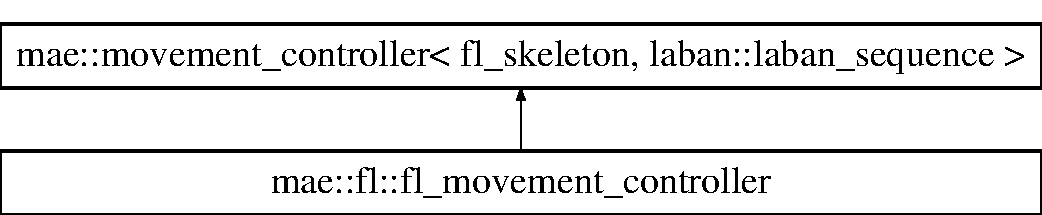
\includegraphics[height=2.000000cm]{classmae_1_1fl_1_1fl__movement__controller}
\end{center}
\end{figure}
\subsection*{Public Member Functions}
\begin{DoxyCompactItemize}
\item 
\hyperlink{classmae_1_1fl_1_1fl__movement__controller_ab2be7883de1d85c282720633014e3ca2}{fl\-\_\-movement\-\_\-controller} (unsigned int pose\-\_\-buffer\-\_\-size=0, double framerate=1.\-0/30.\-0, bool debug=false)
\item 
\hyperlink{classmae_1_1fl_1_1fl__movement__controller_ac72d3642ed9580a6d0b2364aac1c75e4}{fl\-\_\-movement\-\_\-controller} (std\-::vector$<$ \hyperlink{classmae_1_1bone}{bone} $>$ body\-\_\-parts, std\-::vector$<$ std\-::shared\-\_\-ptr$<$ \hyperlink{classmae_1_1fl_1_1laban_1_1column__definition}{laban\-::column\-\_\-definition} $>$ $>$ column\-\_\-definitions, unsigned int pose\-\_\-buffer\-\_\-size=0, unsigned int beats\-\_\-per\-\_\-measure=\hyperlink{classmae_1_1fl_1_1laban_1_1laban__sequence_a2e64362d5cfeb89eb8545cb064e63170}{laban\-::laban\-\_\-sequence\-::default\-\_\-beats\-\_\-per\-\_\-measure}(), unsigned int beat\-\_\-duration=\hyperlink{classmae_1_1fl_1_1laban_1_1laban__sequence_ac7bf04cdac0c3aed6b8ee4a887e561d9}{laban\-::laban\-\_\-sequence\-::default\-\_\-beat\-\_\-duration}(), laban\-::e\-\_\-time\-\_\-unit time\-\_\-unit=\hyperlink{classmae_1_1fl_1_1laban_1_1laban__sequence_ada28215d43d85e983fe6129e9816eed2}{laban\-::laban\-\_\-sequence\-::default\-\_\-time\-\_\-unit}(), double framerate=1.\-0/30.\-0, bool debug=false)
\item 
\hyperlink{classmae_1_1fl_1_1fl__movement__controller_a98b3787f9a66bddd9296b05bc44d530d}{fl\-\_\-movement\-\_\-controller} (std\-::vector$<$ \hyperlink{classmae_1_1bone}{bone} $>$ body\-\_\-parts, std\-::vector$<$ std\-::shared\-\_\-ptr$<$ \hyperlink{classmae_1_1fl_1_1laban_1_1column__definition}{laban\-::column\-\_\-definition} $>$ $>$ column\-\_\-definitions, std\-::shared\-\_\-ptr$<$ \hyperlink{classmae_1_1fl_1_1laban_1_1laban__sequence__generator}{mae\-::fl\-::laban\-::laban\-\_\-sequence\-\_\-generator} $>$ sequence\-\_\-generator, unsigned int pose\-\_\-buffer\-\_\-size=0, unsigned int beats\-\_\-per\-\_\-measure=\hyperlink{classmae_1_1fl_1_1laban_1_1laban__sequence_a2e64362d5cfeb89eb8545cb064e63170}{laban\-::laban\-\_\-sequence\-::default\-\_\-beats\-\_\-per\-\_\-measure}(), unsigned int beat\-\_\-duration=\hyperlink{classmae_1_1fl_1_1laban_1_1laban__sequence_ac7bf04cdac0c3aed6b8ee4a887e561d9}{laban\-::laban\-\_\-sequence\-::default\-\_\-beat\-\_\-duration}(), laban\-::e\-\_\-time\-\_\-unit time\-\_\-unit=\hyperlink{classmae_1_1fl_1_1laban_1_1laban__sequence_ada28215d43d85e983fe6129e9816eed2}{laban\-::laban\-\_\-sequence\-::default\-\_\-time\-\_\-unit}(), double framerate=1.\-0/30.\-0, bool debug=false)
\item 
virtual void \hyperlink{classmae_1_1fl_1_1fl__movement__controller_a3eafa33ebaf85a140bcafdd1670b368c}{next\-\_\-frame} (long timestamp, std\-::shared\-\_\-ptr$<$ \hyperlink{classmae_1_1general__skeleton}{general\-\_\-skeleton} $>$ skeleton)
\item 
virtual void \hyperlink{classmae_1_1fl_1_1fl__movement__controller_a0bdd94f763b740c612475df629dc3bcf}{set\-\_\-recognition\-\_\-tolerance} (double tolerance)
\item 
virtual std\-::shared\-\_\-ptr\\*
$<$ \hyperlink{classmae_1_1fl_1_1laban_1_1laban__sequence__recognizer}{mae\-::fl\-::laban\-::laban\-\_\-sequence\-\_\-recognizer} $>$ \hyperlink{classmae_1_1fl_1_1fl__movement__controller_abaacf2be62b0194ee6ffcac844a09d22}{get\-\_\-laban\-\_\-sequence\-\_\-recognizer} () const 
\item 
virtual std\-::shared\-\_\-ptr\\*
$<$ \hyperlink{classmae_1_1fl_1_1laban_1_1laban__sequence__generator}{mae\-::fl\-::laban\-::laban\-\_\-sequence\-\_\-generator} $>$ \hyperlink{classmae_1_1fl_1_1fl__movement__controller_a4f4390073c34aa18b55a57c447c84542}{get\-\_\-laban\-\_\-sequence\-\_\-generator} () const 
\item 
virtual std\-::shared\-\_\-ptr\\*
$<$ \hyperlink{classmae_1_1fl_1_1fl__pose__detector}{fl\-\_\-pose\-\_\-detector} $>$ \hyperlink{classmae_1_1fl_1_1fl__movement__controller_a0d25a3e53c47e1cb1f0eb3cd7df07548}{get\-\_\-fl\-\_\-pose\-\_\-detector} () const 
\end{DoxyCompactItemize}


\subsection{Constructor \& Destructor Documentation}
\hypertarget{classmae_1_1fl_1_1fl__movement__controller_ab2be7883de1d85c282720633014e3ca2}{\index{mae\-::fl\-::fl\-\_\-movement\-\_\-controller@{mae\-::fl\-::fl\-\_\-movement\-\_\-controller}!fl\-\_\-movement\-\_\-controller@{fl\-\_\-movement\-\_\-controller}}
\index{fl\-\_\-movement\-\_\-controller@{fl\-\_\-movement\-\_\-controller}!mae::fl::fl_movement_controller@{mae\-::fl\-::fl\-\_\-movement\-\_\-controller}}
\subsubsection[{fl\-\_\-movement\-\_\-controller}]{\setlength{\rightskip}{0pt plus 5cm}mae\-::fl\-::fl\-\_\-movement\-\_\-controller\-::fl\-\_\-movement\-\_\-controller (
\begin{DoxyParamCaption}
\item[{unsigned int}]{pose\-\_\-buffer\-\_\-size = {\ttfamily 0}, }
\item[{double}]{framerate = {\ttfamily 1.0/30.0}, }
\item[{bool}]{debug = {\ttfamily false}}
\end{DoxyParamCaption}
)}}\label{classmae_1_1fl_1_1fl__movement__controller_ab2be7883de1d85c282720633014e3ca2}
Creates a new controller for movements analysis based on Labanotation and fl\-\_\-skeletons. The used body parts are assumed to be the default ones used by the N\-I\-T\-E skeleton. Since no column definition is given the default columns are the only ones that can be used.


\begin{DoxyParams}{Parameters}
{\em pose\-\_\-buffer\-\_\-size} & The buffer size for the movement detector (number of frames to process). Values $<$= 1 means calculating the buffer size from the registered sequences. \\
\hline
{\em framerate} & The framerate for the stream. \\
\hline
{\em debug} & True for debug console print. \\
\hline
\end{DoxyParams}
\hypertarget{classmae_1_1fl_1_1fl__movement__controller_ac72d3642ed9580a6d0b2364aac1c75e4}{\index{mae\-::fl\-::fl\-\_\-movement\-\_\-controller@{mae\-::fl\-::fl\-\_\-movement\-\_\-controller}!fl\-\_\-movement\-\_\-controller@{fl\-\_\-movement\-\_\-controller}}
\index{fl\-\_\-movement\-\_\-controller@{fl\-\_\-movement\-\_\-controller}!mae::fl::fl_movement_controller@{mae\-::fl\-::fl\-\_\-movement\-\_\-controller}}
\subsubsection[{fl\-\_\-movement\-\_\-controller}]{\setlength{\rightskip}{0pt plus 5cm}mae\-::fl\-::fl\-\_\-movement\-\_\-controller\-::fl\-\_\-movement\-\_\-controller (
\begin{DoxyParamCaption}
\item[{std\-::vector$<$ {\bf bone} $>$}]{body\-\_\-parts, }
\item[{std\-::vector$<$ std\-::shared\-\_\-ptr$<$ {\bf laban\-::column\-\_\-definition} $>$ $>$}]{column\-\_\-definitions, }
\item[{unsigned int}]{pose\-\_\-buffer\-\_\-size = {\ttfamily 0}, }
\item[{unsigned int}]{beats\-\_\-per\-\_\-measure = {\ttfamily {\bf laban\-::laban\-\_\-sequence\-::default\-\_\-beats\-\_\-per\-\_\-measure}()}, }
\item[{unsigned int}]{beat\-\_\-duration = {\ttfamily {\bf laban\-::laban\-\_\-sequence\-::default\-\_\-beat\-\_\-duration}()}, }
\item[{laban\-::e\-\_\-time\-\_\-unit}]{time\-\_\-unit = {\ttfamily {\bf laban\-::laban\-\_\-sequence\-::default\-\_\-time\-\_\-unit}()}, }
\item[{double}]{framerate = {\ttfamily 1.0/30.0}, }
\item[{bool}]{debug = {\ttfamily false}}
\end{DoxyParamCaption}
)}}\label{classmae_1_1fl_1_1fl__movement__controller_ac72d3642ed9580a6d0b2364aac1c75e4}
Creates a new controller for movements analysis based on Labanotation and fl\-\_\-skeletons which handles the given body parts and uses the defined columns for the Labanotation sequence.


\begin{DoxyParams}{Parameters}
{\em body\-\_\-parts} & The body parts which shall be handled. \\
\hline
{\em column\-\_\-definitions} & The columns which shall be defined besides those that are defined by default. \\
\hline
{\em pose\-\_\-buffer\-\_\-size} & The buffer size for the movement detector (number of frames to process). Values $<$= 1 means calculating the buffer size from the registered sequences. \\
\hline
{\em beats\-\_\-per\-\_\-measure} & The number of beats per measure. \\
\hline
{\em beat\-\_\-duration} & The duration of a single beat. \\
\hline
{\em time\-\_\-unit} & The time unit to be applied. \\
\hline
{\em framerate} & The framerate for the stream. \\
\hline
{\em debug} & True for debug console print. \\
\hline
\end{DoxyParams}
\hypertarget{classmae_1_1fl_1_1fl__movement__controller_a98b3787f9a66bddd9296b05bc44d530d}{\index{mae\-::fl\-::fl\-\_\-movement\-\_\-controller@{mae\-::fl\-::fl\-\_\-movement\-\_\-controller}!fl\-\_\-movement\-\_\-controller@{fl\-\_\-movement\-\_\-controller}}
\index{fl\-\_\-movement\-\_\-controller@{fl\-\_\-movement\-\_\-controller}!mae::fl::fl_movement_controller@{mae\-::fl\-::fl\-\_\-movement\-\_\-controller}}
\subsubsection[{fl\-\_\-movement\-\_\-controller}]{\setlength{\rightskip}{0pt plus 5cm}mae\-::fl\-::fl\-\_\-movement\-\_\-controller\-::fl\-\_\-movement\-\_\-controller (
\begin{DoxyParamCaption}
\item[{std\-::vector$<$ {\bf bone} $>$}]{body\-\_\-parts, }
\item[{std\-::vector$<$ std\-::shared\-\_\-ptr$<$ {\bf laban\-::column\-\_\-definition} $>$ $>$}]{column\-\_\-definitions, }
\item[{std\-::shared\-\_\-ptr$<$ {\bf mae\-::fl\-::laban\-::laban\-\_\-sequence\-\_\-generator} $>$}]{sequence\-\_\-generator, }
\item[{unsigned int}]{pose\-\_\-buffer\-\_\-size = {\ttfamily 0}, }
\item[{unsigned int}]{beats\-\_\-per\-\_\-measure = {\ttfamily {\bf laban\-::laban\-\_\-sequence\-::default\-\_\-beats\-\_\-per\-\_\-measure}()}, }
\item[{unsigned int}]{beat\-\_\-duration = {\ttfamily {\bf laban\-::laban\-\_\-sequence\-::default\-\_\-beat\-\_\-duration}()}, }
\item[{laban\-::e\-\_\-time\-\_\-unit}]{time\-\_\-unit = {\ttfamily {\bf laban\-::laban\-\_\-sequence\-::default\-\_\-time\-\_\-unit}()}, }
\item[{double}]{framerate = {\ttfamily 1.0/30.0}, }
\item[{bool}]{debug = {\ttfamily false}}
\end{DoxyParamCaption}
)}}\label{classmae_1_1fl_1_1fl__movement__controller_a98b3787f9a66bddd9296b05bc44d530d}
Creates a new controller for movements analysis based on Labanotation and fl\-\_\-skeletons which handles the given body parts and uses the defined columns for the Labanotation sequence.


\begin{DoxyParams}{Parameters}
{\em body\-\_\-parts} & The body parts which shall be handled. \\
\hline
{\em column\-\_\-definitions} & The columns which shall be defined besides those that are defined by default. \\
\hline
{\em sequence\-\_\-generator} & \\
\hline
{\em pose\-\_\-buffer\-\_\-size} & The buffer size for the movement detector (number of frames to process). Values $<$= 1 means calculating the buffer size from the registered sequences. \\
\hline
{\em beats\-\_\-per\-\_\-measure} & The number of beats per measure. \\
\hline
{\em beat\-\_\-duration} & The duration of a single beat. \\
\hline
{\em time\-\_\-unit} & The time unit to be applied. \\
\hline
{\em framerate} & The framerate for the stream. \\
\hline
{\em debug} & True for debug console print. \\
\hline
\end{DoxyParams}


\subsection{Member Function Documentation}
\hypertarget{classmae_1_1fl_1_1fl__movement__controller_a0d25a3e53c47e1cb1f0eb3cd7df07548}{\index{mae\-::fl\-::fl\-\_\-movement\-\_\-controller@{mae\-::fl\-::fl\-\_\-movement\-\_\-controller}!get\-\_\-fl\-\_\-pose\-\_\-detector@{get\-\_\-fl\-\_\-pose\-\_\-detector}}
\index{get\-\_\-fl\-\_\-pose\-\_\-detector@{get\-\_\-fl\-\_\-pose\-\_\-detector}!mae::fl::fl_movement_controller@{mae\-::fl\-::fl\-\_\-movement\-\_\-controller}}
\subsubsection[{get\-\_\-fl\-\_\-pose\-\_\-detector}]{\setlength{\rightskip}{0pt plus 5cm}std\-::shared\-\_\-ptr$<$ {\bf fl\-\_\-pose\-\_\-detector} $>$ mae\-::fl\-::fl\-\_\-movement\-\_\-controller\-::get\-\_\-fl\-\_\-pose\-\_\-detector (
\begin{DoxyParamCaption}
{}
\end{DoxyParamCaption}
) const\hspace{0.3cm}{\ttfamily [virtual]}}}\label{classmae_1_1fl_1_1fl__movement__controller_a0d25a3e53c47e1cb1f0eb3cd7df07548}
Returns the fl pose detector.

\begin{DoxyReturn}{Returns}
The detector. 
\end{DoxyReturn}
\hypertarget{classmae_1_1fl_1_1fl__movement__controller_a4f4390073c34aa18b55a57c447c84542}{\index{mae\-::fl\-::fl\-\_\-movement\-\_\-controller@{mae\-::fl\-::fl\-\_\-movement\-\_\-controller}!get\-\_\-laban\-\_\-sequence\-\_\-generator@{get\-\_\-laban\-\_\-sequence\-\_\-generator}}
\index{get\-\_\-laban\-\_\-sequence\-\_\-generator@{get\-\_\-laban\-\_\-sequence\-\_\-generator}!mae::fl::fl_movement_controller@{mae\-::fl\-::fl\-\_\-movement\-\_\-controller}}
\subsubsection[{get\-\_\-laban\-\_\-sequence\-\_\-generator}]{\setlength{\rightskip}{0pt plus 5cm}std\-::shared\-\_\-ptr$<$ {\bf mae\-::fl\-::laban\-::laban\-\_\-sequence\-\_\-generator} $>$ mae\-::fl\-::fl\-\_\-movement\-\_\-controller\-::get\-\_\-laban\-\_\-sequence\-\_\-generator (
\begin{DoxyParamCaption}
{}
\end{DoxyParamCaption}
) const\hspace{0.3cm}{\ttfamily [virtual]}}}\label{classmae_1_1fl_1_1fl__movement__controller_a4f4390073c34aa18b55a57c447c84542}
Returns the laban sequence generator.

\begin{DoxyReturn}{Returns}
The generator. 
\end{DoxyReturn}
\hypertarget{classmae_1_1fl_1_1fl__movement__controller_abaacf2be62b0194ee6ffcac844a09d22}{\index{mae\-::fl\-::fl\-\_\-movement\-\_\-controller@{mae\-::fl\-::fl\-\_\-movement\-\_\-controller}!get\-\_\-laban\-\_\-sequence\-\_\-recognizer@{get\-\_\-laban\-\_\-sequence\-\_\-recognizer}}
\index{get\-\_\-laban\-\_\-sequence\-\_\-recognizer@{get\-\_\-laban\-\_\-sequence\-\_\-recognizer}!mae::fl::fl_movement_controller@{mae\-::fl\-::fl\-\_\-movement\-\_\-controller}}
\subsubsection[{get\-\_\-laban\-\_\-sequence\-\_\-recognizer}]{\setlength{\rightskip}{0pt plus 5cm}std\-::shared\-\_\-ptr$<$ {\bf laban\-::laban\-\_\-sequence\-\_\-recognizer} $>$ mae\-::fl\-::fl\-\_\-movement\-\_\-controller\-::get\-\_\-laban\-\_\-sequence\-\_\-recognizer (
\begin{DoxyParamCaption}
{}
\end{DoxyParamCaption}
) const\hspace{0.3cm}{\ttfamily [virtual]}}}\label{classmae_1_1fl_1_1fl__movement__controller_abaacf2be62b0194ee6ffcac844a09d22}
Returns the laban sequence recognizer.

\begin{DoxyReturn}{Returns}
The recognizer. 
\end{DoxyReturn}
\hypertarget{classmae_1_1fl_1_1fl__movement__controller_a3eafa33ebaf85a140bcafdd1670b368c}{\index{mae\-::fl\-::fl\-\_\-movement\-\_\-controller@{mae\-::fl\-::fl\-\_\-movement\-\_\-controller}!next\-\_\-frame@{next\-\_\-frame}}
\index{next\-\_\-frame@{next\-\_\-frame}!mae::fl::fl_movement_controller@{mae\-::fl\-::fl\-\_\-movement\-\_\-controller}}
\subsubsection[{next\-\_\-frame}]{\setlength{\rightskip}{0pt plus 5cm}void mae\-::fl\-::fl\-\_\-movement\-\_\-controller\-::next\-\_\-frame (
\begin{DoxyParamCaption}
\item[{long}]{timestamp, }
\item[{std\-::shared\-\_\-ptr$<$ {\bf general\-\_\-skeleton} $>$}]{skeleton}
\end{DoxyParamCaption}
)\hspace{0.3cm}{\ttfamily [virtual]}}}\label{classmae_1_1fl_1_1fl__movement__controller_a3eafa33ebaf85a140bcafdd1670b368c}
Invokes the processing for a new frame. The skeleton provides the information which is the basis for any further calculations.


\begin{DoxyParams}{Parameters}
{\em timestamp} & The timestamp on which the skeleton occured. \\
\hline
{\em skeleton} & The skeleton data for the frame. \\
\hline
\end{DoxyParams}
\hypertarget{classmae_1_1fl_1_1fl__movement__controller_a0bdd94f763b740c612475df629dc3bcf}{\index{mae\-::fl\-::fl\-\_\-movement\-\_\-controller@{mae\-::fl\-::fl\-\_\-movement\-\_\-controller}!set\-\_\-recognition\-\_\-tolerance@{set\-\_\-recognition\-\_\-tolerance}}
\index{set\-\_\-recognition\-\_\-tolerance@{set\-\_\-recognition\-\_\-tolerance}!mae::fl::fl_movement_controller@{mae\-::fl\-::fl\-\_\-movement\-\_\-controller}}
\subsubsection[{set\-\_\-recognition\-\_\-tolerance}]{\setlength{\rightskip}{0pt plus 5cm}void mae\-::fl\-::fl\-\_\-movement\-\_\-controller\-::set\-\_\-recognition\-\_\-tolerance (
\begin{DoxyParamCaption}
\item[{double}]{tolerance}
\end{DoxyParamCaption}
)\hspace{0.3cm}{\ttfamily [virtual]}}}\label{classmae_1_1fl_1_1fl__movement__controller_a0bdd94f763b740c612475df629dc3bcf}
Sets the tolerance for the recognition. The tolerance is a value which represents the number of beats of the labanotation which are tolerated in deviation.


\begin{DoxyParams}{Parameters}
{\em tolerance} & The tolerance to be accepted. \\
\hline
\end{DoxyParams}


The documentation for this class was generated from the following files\-:\begin{DoxyCompactItemize}
\item 
src/mae/fl/fl\-\_\-movement\-\_\-controller.\-hpp\item 
src/mae/fl/fl\-\_\-movement\-\_\-controller.\-cpp\end{DoxyCompactItemize}

\hypertarget{classmae_1_1fl_1_1fl__pose__detector}{\section{mae\-:\-:fl\-:\-:fl\-\_\-pose\-\_\-detector Class Reference}
\label{classmae_1_1fl_1_1fl__pose__detector}\index{mae\-::fl\-::fl\-\_\-pose\-\_\-detector@{mae\-::fl\-::fl\-\_\-pose\-\_\-detector}}
}
Inheritance diagram for mae\-:\-:fl\-:\-:fl\-\_\-pose\-\_\-detector\-:\begin{figure}[H]
\begin{center}
\leavevmode
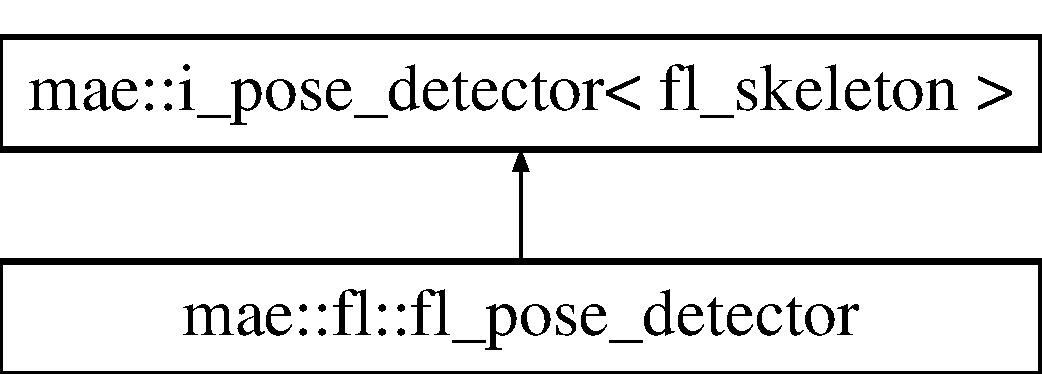
\includegraphics[height=2.000000cm]{classmae_1_1fl_1_1fl__pose__detector}
\end{center}
\end{figure}
\subsection*{Public Member Functions}
\begin{DoxyCompactItemize}
\item 
\hyperlink{classmae_1_1fl_1_1fl__pose__detector_a3e52ce649f55340ebcd5a2fec804278b}{fl\-\_\-pose\-\_\-detector} (double hysteresis\-\_\-val=\hyperlink{classmae_1_1fl_1_1fl__pose__detector_adb2f046d501a87de9e5589b346ef3782}{fl\-\_\-pose\-\_\-detector\-::default\-\_\-hysteresis\-\_\-val}(), bool debug=false)
\item 
virtual void \hyperlink{classmae_1_1fl_1_1fl__pose__detector_a807c41e01fed7a729058b91ff4ff90f3}{set\-\_\-hysteresis\-\_\-val} (double hysteresis\-\_\-val)
\item 
virtual double \hyperlink{classmae_1_1fl_1_1fl__pose__detector_a5347e97f3685d7168a182e7e373f09cf}{get\-\_\-hysteresis\-\_\-val} () const 
\item 
virtual std\-::shared\-\_\-ptr\\*
$<$ \hyperlink{classmae_1_1general__pose}{mae\-::general\-\_\-pose} $>$ \hyperlink{classmae_1_1fl_1_1fl__pose__detector_af8283b9b73fcc1bf7ea5a4220c2ecd55}{pose} (std\-::shared\-\_\-ptr$<$ \hyperlink{classmae_1_1fl_1_1fl__skeleton}{fl\-\_\-skeleton} $>$ skeleton, std\-::vector$<$ \hyperlink{classmae_1_1bone}{bone} $>$ body\-\_\-parts, std\-::shared\-\_\-ptr$<$ \hyperlink{classmae_1_1general__pose}{general\-\_\-pose} $>$ previous\-\_\-pose)
\item 
virtual std\-::shared\-\_\-ptr\\*
$<$ \hyperlink{classmae_1_1general__pose}{mae\-::general\-\_\-pose} $>$ \hyperlink{classmae_1_1fl_1_1fl__pose__detector_ae7f558696efe7f55cf4895bffd234665}{vector\-\_\-pose} (std\-::shared\-\_\-ptr$<$ \hyperlink{classmae_1_1fl_1_1fl__skeleton}{fl\-\_\-skeleton} $>$ skeleton, std\-::vector$<$ \hyperlink{classmae_1_1bone}{bone} $>$ body\-\_\-parts, std\-::shared\-\_\-ptr$<$ \hyperlink{classmae_1_1general__pose}{general\-\_\-pose} $>$ previous\-\_\-pose)
\end{DoxyCompactItemize}
\subsection*{Static Public Member Functions}
\begin{DoxyCompactItemize}
\item 
static double \hyperlink{classmae_1_1fl_1_1fl__pose__detector_adb2f046d501a87de9e5589b346ef3782}{default\-\_\-hysteresis\-\_\-val} ()
\end{DoxyCompactItemize}


\subsection{Constructor \& Destructor Documentation}
\hypertarget{classmae_1_1fl_1_1fl__pose__detector_a3e52ce649f55340ebcd5a2fec804278b}{\index{mae\-::fl\-::fl\-\_\-pose\-\_\-detector@{mae\-::fl\-::fl\-\_\-pose\-\_\-detector}!fl\-\_\-pose\-\_\-detector@{fl\-\_\-pose\-\_\-detector}}
\index{fl\-\_\-pose\-\_\-detector@{fl\-\_\-pose\-\_\-detector}!mae::fl::fl_pose_detector@{mae\-::fl\-::fl\-\_\-pose\-\_\-detector}}
\subsubsection[{fl\-\_\-pose\-\_\-detector}]{\setlength{\rightskip}{0pt plus 5cm}mae\-::fl\-::fl\-\_\-pose\-\_\-detector\-::fl\-\_\-pose\-\_\-detector (
\begin{DoxyParamCaption}
\item[{double}]{hysteresis\-\_\-val = {\ttfamily {\bf fl\-\_\-pose\-\_\-detector\-::default\-\_\-hysteresis\-\_\-val}()}, }
\item[{bool}]{debug = {\ttfamily false}}
\end{DoxyParamCaption}
)}}\label{classmae_1_1fl_1_1fl__pose__detector_a3e52ce649f55340ebcd5a2fec804278b}
Creates a new pose detector.


\begin{DoxyParams}{Parameters}
{\em hysteresis\-\_\-val} & The value applied for the hysteris. 22.\-5 for no hysteresis. \\
\hline
{\em debug} & (optional) If true debug output on the console is done. \\
\hline
\end{DoxyParams}


\subsection{Member Function Documentation}
\hypertarget{classmae_1_1fl_1_1fl__pose__detector_adb2f046d501a87de9e5589b346ef3782}{\index{mae\-::fl\-::fl\-\_\-pose\-\_\-detector@{mae\-::fl\-::fl\-\_\-pose\-\_\-detector}!default\-\_\-hysteresis\-\_\-val@{default\-\_\-hysteresis\-\_\-val}}
\index{default\-\_\-hysteresis\-\_\-val@{default\-\_\-hysteresis\-\_\-val}!mae::fl::fl_pose_detector@{mae\-::fl\-::fl\-\_\-pose\-\_\-detector}}
\subsubsection[{default\-\_\-hysteresis\-\_\-val}]{\setlength{\rightskip}{0pt plus 5cm}double mae\-::fl\-::fl\-\_\-pose\-\_\-detector\-::default\-\_\-hysteresis\-\_\-val (
\begin{DoxyParamCaption}
{}
\end{DoxyParamCaption}
)\hspace{0.3cm}{\ttfamily [static]}}}\label{classmae_1_1fl_1_1fl__pose__detector_adb2f046d501a87de9e5589b346ef3782}
Returns the default hysteresis threshold value.

\begin{DoxyReturn}{Returns}
The default hysteresis threshold value. 
\end{DoxyReturn}
\hypertarget{classmae_1_1fl_1_1fl__pose__detector_a5347e97f3685d7168a182e7e373f09cf}{\index{mae\-::fl\-::fl\-\_\-pose\-\_\-detector@{mae\-::fl\-::fl\-\_\-pose\-\_\-detector}!get\-\_\-hysteresis\-\_\-val@{get\-\_\-hysteresis\-\_\-val}}
\index{get\-\_\-hysteresis\-\_\-val@{get\-\_\-hysteresis\-\_\-val}!mae::fl::fl_pose_detector@{mae\-::fl\-::fl\-\_\-pose\-\_\-detector}}
\subsubsection[{get\-\_\-hysteresis\-\_\-val}]{\setlength{\rightskip}{0pt plus 5cm}double mae\-::fl\-::fl\-\_\-pose\-\_\-detector\-::get\-\_\-hysteresis\-\_\-val (
\begin{DoxyParamCaption}
{}
\end{DoxyParamCaption}
) const\hspace{0.3cm}{\ttfamily [virtual]}}}\label{classmae_1_1fl_1_1fl__pose__detector_a5347e97f3685d7168a182e7e373f09cf}
Returns the hysteresis threshold value.

\begin{DoxyReturn}{Returns}
The value. 
\end{DoxyReturn}
\hypertarget{classmae_1_1fl_1_1fl__pose__detector_af8283b9b73fcc1bf7ea5a4220c2ecd55}{\index{mae\-::fl\-::fl\-\_\-pose\-\_\-detector@{mae\-::fl\-::fl\-\_\-pose\-\_\-detector}!pose@{pose}}
\index{pose@{pose}!mae::fl::fl_pose_detector@{mae\-::fl\-::fl\-\_\-pose\-\_\-detector}}
\subsubsection[{pose}]{\setlength{\rightskip}{0pt plus 5cm}std\-::shared\-\_\-ptr$<$ {\bf general\-\_\-pose} $>$ mae\-::fl\-::fl\-\_\-pose\-\_\-detector\-::pose (
\begin{DoxyParamCaption}
\item[{std\-::shared\-\_\-ptr$<$ {\bf fl\-\_\-skeleton} $>$}]{skeleton, }
\item[{std\-::vector$<$ {\bf bone} $>$}]{body\-\_\-parts, }
\item[{std\-::shared\-\_\-ptr$<$ {\bf general\-\_\-pose} $>$}]{previous\-\_\-pose}
\end{DoxyParamCaption}
)\hspace{0.3cm}{\ttfamily [virtual]}}}\label{classmae_1_1fl_1_1fl__pose__detector_af8283b9b73fcc1bf7ea5a4220c2ecd55}
Processes the skeleton in order to return the pose for each body part.


\begin{DoxyParams}{Parameters}
{\em skeleton} & The skeleton. \\
\hline
{\em body\-\_\-parts} & The processed body parts. \\
\hline
{\em previous\-\_\-pose} & The previous pose that can be used for hysteresis. \\
\hline
\end{DoxyParams}
\begin{DoxyReturn}{Returns}
The pose. 
\end{DoxyReturn}
\hypertarget{classmae_1_1fl_1_1fl__pose__detector_a807c41e01fed7a729058b91ff4ff90f3}{\index{mae\-::fl\-::fl\-\_\-pose\-\_\-detector@{mae\-::fl\-::fl\-\_\-pose\-\_\-detector}!set\-\_\-hysteresis\-\_\-val@{set\-\_\-hysteresis\-\_\-val}}
\index{set\-\_\-hysteresis\-\_\-val@{set\-\_\-hysteresis\-\_\-val}!mae::fl::fl_pose_detector@{mae\-::fl\-::fl\-\_\-pose\-\_\-detector}}
\subsubsection[{set\-\_\-hysteresis\-\_\-val}]{\setlength{\rightskip}{0pt plus 5cm}void mae\-::fl\-::fl\-\_\-pose\-\_\-detector\-::set\-\_\-hysteresis\-\_\-val (
\begin{DoxyParamCaption}
\item[{double}]{hysteresis\-\_\-val}
\end{DoxyParamCaption}
)\hspace{0.3cm}{\ttfamily [virtual]}}}\label{classmae_1_1fl_1_1fl__pose__detector_a807c41e01fed7a729058b91ff4ff90f3}
Sets the hysteresis threshold value.


\begin{DoxyParams}{Parameters}
{\em hysteresis\-\_\-val} & The value. \\
\hline
\end{DoxyParams}
\hypertarget{classmae_1_1fl_1_1fl__pose__detector_ae7f558696efe7f55cf4895bffd234665}{\index{mae\-::fl\-::fl\-\_\-pose\-\_\-detector@{mae\-::fl\-::fl\-\_\-pose\-\_\-detector}!vector\-\_\-pose@{vector\-\_\-pose}}
\index{vector\-\_\-pose@{vector\-\_\-pose}!mae::fl::fl_pose_detector@{mae\-::fl\-::fl\-\_\-pose\-\_\-detector}}
\subsubsection[{vector\-\_\-pose}]{\setlength{\rightskip}{0pt plus 5cm}std\-::shared\-\_\-ptr$<$ {\bf mae\-::general\-\_\-pose} $>$ mae\-::fl\-::fl\-\_\-pose\-\_\-detector\-::vector\-\_\-pose (
\begin{DoxyParamCaption}
\item[{std\-::shared\-\_\-ptr$<$ {\bf fl\-\_\-skeleton} $>$}]{skeleton, }
\item[{std\-::vector$<$ {\bf bone} $>$}]{body\-\_\-parts, }
\item[{std\-::shared\-\_\-ptr$<$ {\bf general\-\_\-pose} $>$}]{previous\-\_\-pose}
\end{DoxyParamCaption}
)\hspace{0.3cm}{\ttfamily [virtual]}}}\label{classmae_1_1fl_1_1fl__pose__detector_ae7f558696efe7f55cf4895bffd234665}
Returns a vector pose which means calculating the pose from the vectors not from angles.


\begin{DoxyParams}{Parameters}
{\em skeleton} & The skeleton. \\
\hline
{\em body\-\_\-parts} & The processed body parts. \\
\hline
{\em previous\-\_\-pose} & The previous pose that can be used for hysteresis. \\
\hline
\end{DoxyParams}
\begin{DoxyReturn}{Returns}
The pose. 
\end{DoxyReturn}


The documentation for this class was generated from the following files\-:\begin{DoxyCompactItemize}
\item 
src/mae/fl/fl\-\_\-pose\-\_\-detector.\-hpp\item 
src/mae/fl/fl\-\_\-pose\-\_\-detector.\-cpp\end{DoxyCompactItemize}

\hypertarget{classmae_1_1fl_1_1fl__skeleton}{\section{mae\-:\-:fl\-:\-:fl\-\_\-skeleton Class Reference}
\label{classmae_1_1fl_1_1fl__skeleton}\index{mae\-::fl\-::fl\-\_\-skeleton@{mae\-::fl\-::fl\-\_\-skeleton}}
}
Inheritance diagram for mae\-:\-:fl\-:\-:fl\-\_\-skeleton\-:\begin{figure}[H]
\begin{center}
\leavevmode
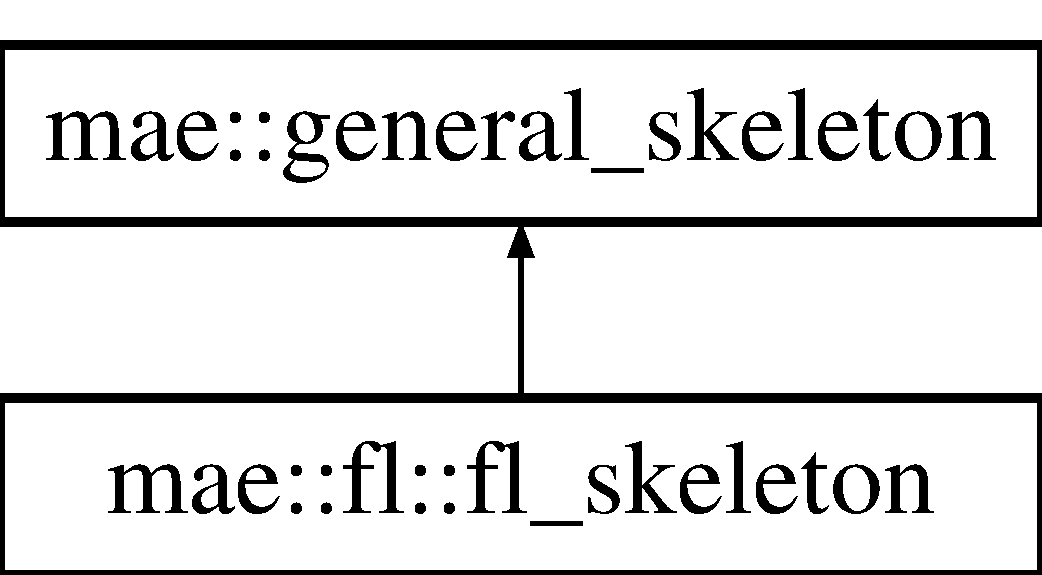
\includegraphics[height=2.000000cm]{classmae_1_1fl_1_1fl__skeleton}
\end{center}
\end{figure}
\subsection*{Public Member Functions}
\begin{DoxyCompactItemize}
\item 
\hyperlink{classmae_1_1fl_1_1fl__skeleton_ac6aa84119ffc3503a1176bbfdf839b76}{fl\-\_\-skeleton} ()
\item 
virtual void \hyperlink{classmae_1_1fl_1_1fl__skeleton_a4dc318fab1376fd9622808f627353f8e}{set\-\_\-torso\-\_\-basis} (std\-::shared\-\_\-ptr$<$ \hyperlink{classmae_1_1math_1_1basis}{mae\-::math\-::basis} $>$ torso\-\_\-basis)
\item 
virtual std\-::shared\-\_\-ptr\\*
$<$ \hyperlink{classmae_1_1math_1_1basis}{mae\-::math\-::basis} $>$ \hyperlink{classmae_1_1fl_1_1fl__skeleton_ad6c54f3187f2497f5f33200baf7e65d1}{get\-\_\-torso\-\_\-basis} () const 
\item 
virtual void \hyperlink{classmae_1_1fl_1_1fl__skeleton_a59ee34f7cf3bff5c97740def6aaa47cb}{set\-\_\-orig\-\_\-skeleton} (std\-::shared\-\_\-ptr$<$ \hyperlink{classmae_1_1general__skeleton}{general\-\_\-skeleton} $>$ offset\-\_\-skeleton)
\item 
virtual std\-::shared\-\_\-ptr\\*
$<$ \hyperlink{classmae_1_1general__skeleton}{general\-\_\-skeleton} $>$ \hyperlink{classmae_1_1fl_1_1fl__skeleton_a69891a8e74b69088706623e671ac0db0}{get\-\_\-orig\-\_\-skeleton} () const 
\item 
virtual std\-::string \hyperlink{classmae_1_1fl_1_1fl__skeleton_ad759f12bd33a9b0fd801eab2018c64de}{str} () const 
\end{DoxyCompactItemize}
\subsection*{Friends}
\begin{DoxyCompactItemize}
\item 
std\-::ostream \& \hyperlink{classmae_1_1fl_1_1fl__skeleton_a95653ccf29a001afd235275601bba323}{operator$<$$<$} (std\-::ostream \&os, const std\-::shared\-\_\-ptr$<$ \hyperlink{classmae_1_1fl_1_1fl__skeleton}{fl\-\_\-skeleton} $>$ \&obj)
\end{DoxyCompactItemize}


\subsection{Constructor \& Destructor Documentation}
\hypertarget{classmae_1_1fl_1_1fl__skeleton_ac6aa84119ffc3503a1176bbfdf839b76}{\index{mae\-::fl\-::fl\-\_\-skeleton@{mae\-::fl\-::fl\-\_\-skeleton}!fl\-\_\-skeleton@{fl\-\_\-skeleton}}
\index{fl\-\_\-skeleton@{fl\-\_\-skeleton}!mae::fl::fl_skeleton@{mae\-::fl\-::fl\-\_\-skeleton}}
\subsubsection[{fl\-\_\-skeleton}]{\setlength{\rightskip}{0pt plus 5cm}mae\-::fl\-::fl\-\_\-skeleton\-::fl\-\_\-skeleton (
\begin{DoxyParamCaption}
{}
\end{DoxyParamCaption}
)}}\label{classmae_1_1fl_1_1fl__skeleton_ac6aa84119ffc3503a1176bbfdf839b76}
Generates a \hyperlink{classmae_1_1fl_1_1fl__skeleton}{fl\-\_\-skeleton} which is the offset skeleton.

The root joint is used to define the offset of the whole skeleton in x,y,z world coordinates. All other joints are given by offset to their parent in the u,r,t object coordinates. 

\subsection{Member Function Documentation}
\hypertarget{classmae_1_1fl_1_1fl__skeleton_a69891a8e74b69088706623e671ac0db0}{\index{mae\-::fl\-::fl\-\_\-skeleton@{mae\-::fl\-::fl\-\_\-skeleton}!get\-\_\-orig\-\_\-skeleton@{get\-\_\-orig\-\_\-skeleton}}
\index{get\-\_\-orig\-\_\-skeleton@{get\-\_\-orig\-\_\-skeleton}!mae::fl::fl_skeleton@{mae\-::fl\-::fl\-\_\-skeleton}}
\subsubsection[{get\-\_\-orig\-\_\-skeleton}]{\setlength{\rightskip}{0pt plus 5cm}std\-::shared\-\_\-ptr$<$ {\bf general\-\_\-skeleton} $>$ mae\-::fl\-::fl\-\_\-skeleton\-::get\-\_\-orig\-\_\-skeleton (
\begin{DoxyParamCaption}
{}
\end{DoxyParamCaption}
) const\hspace{0.3cm}{\ttfamily [virtual]}}}\label{classmae_1_1fl_1_1fl__skeleton_a69891a8e74b69088706623e671ac0db0}
Returns the original general skeleton.

\begin{DoxyReturn}{Returns}
A shared pointer to the general skeleton. 
\end{DoxyReturn}
\hypertarget{classmae_1_1fl_1_1fl__skeleton_ad6c54f3187f2497f5f33200baf7e65d1}{\index{mae\-::fl\-::fl\-\_\-skeleton@{mae\-::fl\-::fl\-\_\-skeleton}!get\-\_\-torso\-\_\-basis@{get\-\_\-torso\-\_\-basis}}
\index{get\-\_\-torso\-\_\-basis@{get\-\_\-torso\-\_\-basis}!mae::fl::fl_skeleton@{mae\-::fl\-::fl\-\_\-skeleton}}
\subsubsection[{get\-\_\-torso\-\_\-basis}]{\setlength{\rightskip}{0pt plus 5cm}std\-::shared\-\_\-ptr$<$ {\bf mae\-::math\-::basis} $>$ mae\-::fl\-::fl\-\_\-skeleton\-::get\-\_\-torso\-\_\-basis (
\begin{DoxyParamCaption}
{}
\end{DoxyParamCaption}
) const\hspace{0.3cm}{\ttfamily [virtual]}}}\label{classmae_1_1fl_1_1fl__skeleton_ad6c54f3187f2497f5f33200baf7e65d1}
Returns the torso basis.

The directions are\-: u The top-\/down or weight direction. r The right-\/left direction. t The direction standing on u and r (pointing from torso to the front).

\begin{DoxyReturn}{Returns}
The torso basis. 
\end{DoxyReturn}
\hypertarget{classmae_1_1fl_1_1fl__skeleton_a59ee34f7cf3bff5c97740def6aaa47cb}{\index{mae\-::fl\-::fl\-\_\-skeleton@{mae\-::fl\-::fl\-\_\-skeleton}!set\-\_\-orig\-\_\-skeleton@{set\-\_\-orig\-\_\-skeleton}}
\index{set\-\_\-orig\-\_\-skeleton@{set\-\_\-orig\-\_\-skeleton}!mae::fl::fl_skeleton@{mae\-::fl\-::fl\-\_\-skeleton}}
\subsubsection[{set\-\_\-orig\-\_\-skeleton}]{\setlength{\rightskip}{0pt plus 5cm}void mae\-::fl\-::fl\-\_\-skeleton\-::set\-\_\-orig\-\_\-skeleton (
\begin{DoxyParamCaption}
\item[{std\-::shared\-\_\-ptr$<$ {\bf general\-\_\-skeleton} $>$}]{offset\-\_\-skeleton}
\end{DoxyParamCaption}
)\hspace{0.3cm}{\ttfamily [virtual]}}}\label{classmae_1_1fl_1_1fl__skeleton_a59ee34f7cf3bff5c97740def6aaa47cb}
Sets the original general skeleton.


\begin{DoxyParams}{Parameters}
{\em offset\-\_\-skeleton} & A shared pointer to the general skeleton. \\
\hline
\end{DoxyParams}
\hypertarget{classmae_1_1fl_1_1fl__skeleton_a4dc318fab1376fd9622808f627353f8e}{\index{mae\-::fl\-::fl\-\_\-skeleton@{mae\-::fl\-::fl\-\_\-skeleton}!set\-\_\-torso\-\_\-basis@{set\-\_\-torso\-\_\-basis}}
\index{set\-\_\-torso\-\_\-basis@{set\-\_\-torso\-\_\-basis}!mae::fl::fl_skeleton@{mae\-::fl\-::fl\-\_\-skeleton}}
\subsubsection[{set\-\_\-torso\-\_\-basis}]{\setlength{\rightskip}{0pt plus 5cm}void mae\-::fl\-::fl\-\_\-skeleton\-::set\-\_\-torso\-\_\-basis (
\begin{DoxyParamCaption}
\item[{std\-::shared\-\_\-ptr$<$ {\bf mae\-::math\-::basis} $>$}]{torso\-\_\-basis}
\end{DoxyParamCaption}
)\hspace{0.3cm}{\ttfamily [virtual]}}}\label{classmae_1_1fl_1_1fl__skeleton_a4dc318fab1376fd9622808f627353f8e}
Sets the torso basis.

The directions are\-: u The top-\/down or weight direction. r The right-\/left direction. t The direction standing on u and r (pointing from torso to the front).


\begin{DoxyParams}{Parameters}
{\em torso\-\_\-basis} & The torso basis. \\
\hline
\end{DoxyParams}
\hypertarget{classmae_1_1fl_1_1fl__skeleton_ad759f12bd33a9b0fd801eab2018c64de}{\index{mae\-::fl\-::fl\-\_\-skeleton@{mae\-::fl\-::fl\-\_\-skeleton}!str@{str}}
\index{str@{str}!mae::fl::fl_skeleton@{mae\-::fl\-::fl\-\_\-skeleton}}
\subsubsection[{str}]{\setlength{\rightskip}{0pt plus 5cm}std\-::string mae\-::fl\-::fl\-\_\-skeleton\-::str (
\begin{DoxyParamCaption}
{}
\end{DoxyParamCaption}
) const\hspace{0.3cm}{\ttfamily [virtual]}}}\label{classmae_1_1fl_1_1fl__skeleton_ad759f12bd33a9b0fd801eab2018c64de}
Converts this object to a string.

\begin{DoxyReturn}{Returns}
This object as a string. 
\end{DoxyReturn}


Reimplemented from \hyperlink{classmae_1_1general__skeleton_a583f49cd26231afbaf9e45decd593f11}{mae\-::general\-\_\-skeleton}.



\subsection{Friends And Related Function Documentation}
\hypertarget{classmae_1_1fl_1_1fl__skeleton_a95653ccf29a001afd235275601bba323}{\index{mae\-::fl\-::fl\-\_\-skeleton@{mae\-::fl\-::fl\-\_\-skeleton}!operator$<$$<$@{operator$<$$<$}}
\index{operator$<$$<$@{operator$<$$<$}!mae::fl::fl_skeleton@{mae\-::fl\-::fl\-\_\-skeleton}}
\subsubsection[{operator$<$$<$}]{\setlength{\rightskip}{0pt plus 5cm}std\-::ostream\& operator$<$$<$ (
\begin{DoxyParamCaption}
\item[{std\-::ostream \&}]{os, }
\item[{const std\-::shared\-\_\-ptr$<$ {\bf fl\-\_\-skeleton} $>$ \&}]{obj}
\end{DoxyParamCaption}
)\hspace{0.3cm}{\ttfamily [friend]}}}\label{classmae_1_1fl_1_1fl__skeleton_a95653ccf29a001afd235275601bba323}
Prints this object tot the stream.


\begin{DoxyParams}{Parameters}
{\em os} & \\
\hline
{\em obj} & \\
\hline
\end{DoxyParams}
\begin{DoxyReturn}{Returns}

\end{DoxyReturn}


The documentation for this class was generated from the following files\-:\begin{DoxyCompactItemize}
\item 
src/mae/fl/fl\-\_\-skeleton.\-hpp\item 
src/mae/fl/fl\-\_\-skeleton.\-cpp\end{DoxyCompactItemize}

\hypertarget{classmae_1_1fl_1_1fl__skeleton__controller}{\section{mae\-:\-:fl\-:\-:fl\-\_\-skeleton\-\_\-controller Class Reference}
\label{classmae_1_1fl_1_1fl__skeleton__controller}\index{mae\-::fl\-::fl\-\_\-skeleton\-\_\-controller@{mae\-::fl\-::fl\-\_\-skeleton\-\_\-controller}}
}
Inheritance diagram for mae\-:\-:fl\-:\-:fl\-\_\-skeleton\-\_\-controller\-:\begin{figure}[H]
\begin{center}
\leavevmode
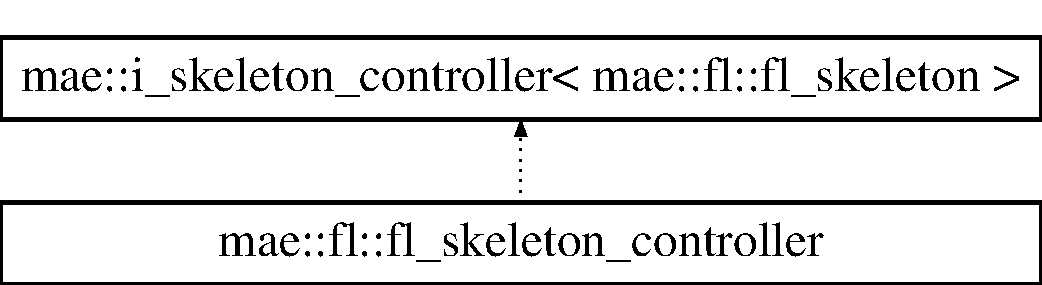
\includegraphics[height=2.000000cm]{classmae_1_1fl_1_1fl__skeleton__controller}
\end{center}
\end{figure}
\subsection*{Public Member Functions}
\begin{DoxyCompactItemize}
\item 
\hyperlink{classmae_1_1fl_1_1fl__skeleton__controller_a217858c5469e4d278d7b50b36750edd9}{fl\-\_\-skeleton\-\_\-controller} (bool debug=false)
\item 
virtual std\-::shared\-\_\-ptr\\*
$<$ \hyperlink{classmae_1_1fl_1_1fl__skeleton}{fl\-\_\-skeleton} $>$ \hyperlink{classmae_1_1fl_1_1fl__skeleton__controller_a0775153d13e802f14d2df3b5bcb51ff1}{specified\-\_\-skeleton} (std\-::shared\-\_\-ptr$<$ \hyperlink{classmae_1_1general__skeleton}{general\-\_\-skeleton} $>$ skeleton)
\item 
virtual std\-::shared\-\_\-ptr\\*
$<$ \hyperlink{classmae_1_1fl_1_1fl__skeleton}{fl\-\_\-skeleton} $>$ \hyperlink{classmae_1_1fl_1_1fl__skeleton__controller_a56a49213e8c75d8a659148965413a5a6}{specified\-\_\-skeleton} (std\-::shared\-\_\-ptr$<$ \hyperlink{classmae_1_1general__skeleton}{general\-\_\-skeleton} $>$ skeleton, std\-::shared\-\_\-ptr$<$ \hyperlink{classmae_1_1math_1_1basis}{mae\-::math\-::basis} $>$ torso\-\_\-basis)
\item 
virtual std\-::shared\-\_\-ptr\\*
$<$ \hyperlink{classmae_1_1math_1_1basis}{mae\-::math\-::basis} $>$ \hyperlink{classmae_1_1fl_1_1fl__skeleton__controller_a54cfb81a3be142676d73654b271b46c2}{create\-\_\-torso\-\_\-basis} (std\-::shared\-\_\-ptr$<$ \hyperlink{classmae_1_1general__skeleton}{general\-\_\-skeleton} $>$ skeleton)
\end{DoxyCompactItemize}


\subsection{Constructor \& Destructor Documentation}
\hypertarget{classmae_1_1fl_1_1fl__skeleton__controller_a217858c5469e4d278d7b50b36750edd9}{\index{mae\-::fl\-::fl\-\_\-skeleton\-\_\-controller@{mae\-::fl\-::fl\-\_\-skeleton\-\_\-controller}!fl\-\_\-skeleton\-\_\-controller@{fl\-\_\-skeleton\-\_\-controller}}
\index{fl\-\_\-skeleton\-\_\-controller@{fl\-\_\-skeleton\-\_\-controller}!mae::fl::fl_skeleton_controller@{mae\-::fl\-::fl\-\_\-skeleton\-\_\-controller}}
\subsubsection[{fl\-\_\-skeleton\-\_\-controller}]{\setlength{\rightskip}{0pt plus 5cm}mae\-::fl\-::fl\-\_\-skeleton\-\_\-controller\-::fl\-\_\-skeleton\-\_\-controller (
\begin{DoxyParamCaption}
\item[{bool}]{debug = {\ttfamily false}}
\end{DoxyParamCaption}
)}}\label{classmae_1_1fl_1_1fl__skeleton__controller_a217858c5469e4d278d7b50b36750edd9}
Create a new skeleton controller which generates a \hyperlink{classmae_1_1fl_1_1fl__skeleton}{fl\-\_\-skeleton} from the general skeleton.


\begin{DoxyParams}{Parameters}
{\em debug} & (optional) If true debug output will be printed to the terminal. \\
\hline
\end{DoxyParams}


\subsection{Member Function Documentation}
\hypertarget{classmae_1_1fl_1_1fl__skeleton__controller_a54cfb81a3be142676d73654b271b46c2}{\index{mae\-::fl\-::fl\-\_\-skeleton\-\_\-controller@{mae\-::fl\-::fl\-\_\-skeleton\-\_\-controller}!create\-\_\-torso\-\_\-basis@{create\-\_\-torso\-\_\-basis}}
\index{create\-\_\-torso\-\_\-basis@{create\-\_\-torso\-\_\-basis}!mae::fl::fl_skeleton_controller@{mae\-::fl\-::fl\-\_\-skeleton\-\_\-controller}}
\subsubsection[{create\-\_\-torso\-\_\-basis}]{\setlength{\rightskip}{0pt plus 5cm}std\-::shared\-\_\-ptr$<$ {\bf mae\-::math\-::basis} $>$ mae\-::fl\-::fl\-\_\-skeleton\-\_\-controller\-::create\-\_\-torso\-\_\-basis (
\begin{DoxyParamCaption}
\item[{std\-::shared\-\_\-ptr$<$ {\bf general\-\_\-skeleton} $>$}]{skeleton}
\end{DoxyParamCaption}
)\hspace{0.3cm}{\ttfamily [virtual]}}}\label{classmae_1_1fl_1_1fl__skeleton__controller_a54cfb81a3be142676d73654b271b46c2}
Creates the torso basis for the given general skeleton.


\begin{DoxyParams}{Parameters}
{\em skeleton} & The skeleton. \\
\hline
\end{DoxyParams}
\begin{DoxyReturn}{Returns}
The torso basis. 
\end{DoxyReturn}
\hypertarget{classmae_1_1fl_1_1fl__skeleton__controller_a0775153d13e802f14d2df3b5bcb51ff1}{\index{mae\-::fl\-::fl\-\_\-skeleton\-\_\-controller@{mae\-::fl\-::fl\-\_\-skeleton\-\_\-controller}!specified\-\_\-skeleton@{specified\-\_\-skeleton}}
\index{specified\-\_\-skeleton@{specified\-\_\-skeleton}!mae::fl::fl_skeleton_controller@{mae\-::fl\-::fl\-\_\-skeleton\-\_\-controller}}
\subsubsection[{specified\-\_\-skeleton}]{\setlength{\rightskip}{0pt plus 5cm}std\-::shared\-\_\-ptr$<$ {\bf fl\-\_\-skeleton} $>$ mae\-::fl\-::fl\-\_\-skeleton\-\_\-controller\-::specified\-\_\-skeleton (
\begin{DoxyParamCaption}
\item[{std\-::shared\-\_\-ptr$<$ {\bf general\-\_\-skeleton} $>$}]{skeleton}
\end{DoxyParamCaption}
)\hspace{0.3cm}{\ttfamily [virtual]}}}\label{classmae_1_1fl_1_1fl__skeleton__controller_a0775153d13e802f14d2df3b5bcb51ff1}
Generates the specified skeleton from the general skeleton.


\begin{DoxyParams}{Parameters}
{\em skeleton} & The general skeleton. \\
\hline
\end{DoxyParams}
\begin{DoxyReturn}{Returns}
The specified skeleton. 
\end{DoxyReturn}


Implements \hyperlink{classmae_1_1i__skeleton__controller_a5142885efc960951334765e2c66052c2}{mae\-::i\-\_\-skeleton\-\_\-controller$<$ mae\-::fl\-::fl\-\_\-skeleton $>$}.

\hypertarget{classmae_1_1fl_1_1fl__skeleton__controller_a56a49213e8c75d8a659148965413a5a6}{\index{mae\-::fl\-::fl\-\_\-skeleton\-\_\-controller@{mae\-::fl\-::fl\-\_\-skeleton\-\_\-controller}!specified\-\_\-skeleton@{specified\-\_\-skeleton}}
\index{specified\-\_\-skeleton@{specified\-\_\-skeleton}!mae::fl::fl_skeleton_controller@{mae\-::fl\-::fl\-\_\-skeleton\-\_\-controller}}
\subsubsection[{specified\-\_\-skeleton}]{\setlength{\rightskip}{0pt plus 5cm}std\-::shared\-\_\-ptr$<$ {\bf fl\-\_\-skeleton} $>$ mae\-::fl\-::fl\-\_\-skeleton\-\_\-controller\-::specified\-\_\-skeleton (
\begin{DoxyParamCaption}
\item[{std\-::shared\-\_\-ptr$<$ {\bf general\-\_\-skeleton} $>$}]{skeleton, }
\item[{std\-::shared\-\_\-ptr$<$ {\bf mae\-::math\-::basis} $>$}]{torso\-\_\-basis}
\end{DoxyParamCaption}
)\hspace{0.3cm}{\ttfamily [virtual]}}}\label{classmae_1_1fl_1_1fl__skeleton__controller_a56a49213e8c75d8a659148965413a5a6}
Generates the specified skeleton from the general skeleton using the given torso basis.


\begin{DoxyParams}{Parameters}
{\em skeleton} & The skeleton to be translated. \\
\hline
{\em torso\-\_\-basis} & The torso basis meant to be used. \\
\hline
\end{DoxyParams}
\begin{DoxyReturn}{Returns}
The specified skeleton. 
\end{DoxyReturn}


The documentation for this class was generated from the following files\-:\begin{DoxyCompactItemize}
\item 
src/mae/fl/fl\-\_\-skeleton\-\_\-controller.\-hpp\item 
src/mae/fl/fl\-\_\-skeleton\-\_\-controller.\-cpp\end{DoxyCompactItemize}

\hypertarget{classmae_1_1general__enriched__pose}{\section{mae\-:\-:general\-\_\-enriched\-\_\-pose Class Reference}
\label{classmae_1_1general__enriched__pose}\index{mae\-::general\-\_\-enriched\-\_\-pose@{mae\-::general\-\_\-enriched\-\_\-pose}}
}
Inheritance diagram for mae\-:\-:general\-\_\-enriched\-\_\-pose\-:\begin{figure}[H]
\begin{center}
\leavevmode
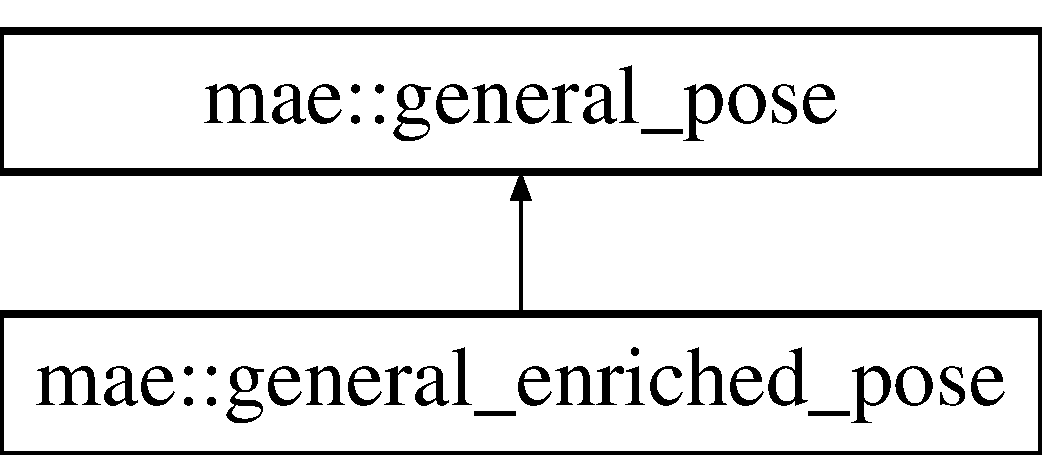
\includegraphics[height=2.000000cm]{classmae_1_1general__enriched__pose}
\end{center}
\end{figure}
\subsection*{Public Member Functions}
\begin{DoxyCompactItemize}
\item 
\hyperlink{classmae_1_1general__enriched__pose_a3b4b9e81621a54059679e2746a760d74}{general\-\_\-enriched\-\_\-pose} ()
\item 
\hyperlink{classmae_1_1general__enriched__pose_ab0656b1482a47c43f1d04be2b457b8ca}{general\-\_\-enriched\-\_\-pose} (std\-::shared\-\_\-ptr$<$ \hyperlink{classmae_1_1general__pose}{general\-\_\-pose} $>$ pose)
\item 
virtual void \hyperlink{classmae_1_1general__enriched__pose_ac6dabf701b6a352b669bf11335827da2}{set\-\_\-key\-\_\-pose} (int body\-\_\-part, bool \hyperlink{classmae_1_1general__enriched__pose_aeb367ce952171488fb93c5bc84d1f0df}{is\-\_\-key\-\_\-pose})
\item 
virtual bool \hyperlink{classmae_1_1general__enriched__pose_aeb367ce952171488fb93c5bc84d1f0df}{is\-\_\-key\-\_\-pose} (int body\-\_\-part)
\item 
virtual void \hyperlink{classmae_1_1general__enriched__pose_a5247ebb0b3f6b2d83a19705c3748ce12}{set\-\_\-in\-\_\-motion} (int body\-\_\-part, bool \hyperlink{classmae_1_1general__enriched__pose_a7a5928c1984b86377dcf038cd550af04}{is\-\_\-in\-\_\-motion})
\item 
virtual bool \hyperlink{classmae_1_1general__enriched__pose_a7a5928c1984b86377dcf038cd550af04}{is\-\_\-in\-\_\-motion} (int body\-\_\-part)
\end{DoxyCompactItemize}


\subsection{Constructor \& Destructor Documentation}
\hypertarget{classmae_1_1general__enriched__pose_a3b4b9e81621a54059679e2746a760d74}{\index{mae\-::general\-\_\-enriched\-\_\-pose@{mae\-::general\-\_\-enriched\-\_\-pose}!general\-\_\-enriched\-\_\-pose@{general\-\_\-enriched\-\_\-pose}}
\index{general\-\_\-enriched\-\_\-pose@{general\-\_\-enriched\-\_\-pose}!mae::general_enriched_pose@{mae\-::general\-\_\-enriched\-\_\-pose}}
\subsubsection[{general\-\_\-enriched\-\_\-pose}]{\setlength{\rightskip}{0pt plus 5cm}mae\-::general\-\_\-enriched\-\_\-pose\-::general\-\_\-enriched\-\_\-pose (
\begin{DoxyParamCaption}
{}
\end{DoxyParamCaption}
)}}\label{classmae_1_1general__enriched__pose_a3b4b9e81621a54059679e2746a760d74}
Creates an enriched pose. \hypertarget{classmae_1_1general__enriched__pose_ab0656b1482a47c43f1d04be2b457b8ca}{\index{mae\-::general\-\_\-enriched\-\_\-pose@{mae\-::general\-\_\-enriched\-\_\-pose}!general\-\_\-enriched\-\_\-pose@{general\-\_\-enriched\-\_\-pose}}
\index{general\-\_\-enriched\-\_\-pose@{general\-\_\-enriched\-\_\-pose}!mae::general_enriched_pose@{mae\-::general\-\_\-enriched\-\_\-pose}}
\subsubsection[{general\-\_\-enriched\-\_\-pose}]{\setlength{\rightskip}{0pt plus 5cm}mae\-::general\-\_\-enriched\-\_\-pose\-::general\-\_\-enriched\-\_\-pose (
\begin{DoxyParamCaption}
\item[{std\-::shared\-\_\-ptr$<$ {\bf general\-\_\-pose} $>$}]{pose}
\end{DoxyParamCaption}
)}}\label{classmae_1_1general__enriched__pose_ab0656b1482a47c43f1d04be2b457b8ca}
Creates an enriched pose from the general pose.


\begin{DoxyParams}{Parameters}
{\em pose} & The general pose. \\
\hline
\end{DoxyParams}


\subsection{Member Function Documentation}
\hypertarget{classmae_1_1general__enriched__pose_a7a5928c1984b86377dcf038cd550af04}{\index{mae\-::general\-\_\-enriched\-\_\-pose@{mae\-::general\-\_\-enriched\-\_\-pose}!is\-\_\-in\-\_\-motion@{is\-\_\-in\-\_\-motion}}
\index{is\-\_\-in\-\_\-motion@{is\-\_\-in\-\_\-motion}!mae::general_enriched_pose@{mae\-::general\-\_\-enriched\-\_\-pose}}
\subsubsection[{is\-\_\-in\-\_\-motion}]{\setlength{\rightskip}{0pt plus 5cm}bool mae\-::general\-\_\-enriched\-\_\-pose\-::is\-\_\-in\-\_\-motion (
\begin{DoxyParamCaption}
\item[{int}]{body\-\_\-part}
\end{DoxyParamCaption}
)\hspace{0.3cm}{\ttfamily [virtual]}}}\label{classmae_1_1general__enriched__pose_a7a5928c1984b86377dcf038cd550af04}
Returns true if this pose is the start of a new motion sequence on the body part..


\begin{DoxyParams}{Parameters}
{\em body\-\_\-part} & The addressed body part. \\
\hline
\end{DoxyParams}
\begin{DoxyReturn}{Returns}
True if motion begin. 
\end{DoxyReturn}
\hypertarget{classmae_1_1general__enriched__pose_aeb367ce952171488fb93c5bc84d1f0df}{\index{mae\-::general\-\_\-enriched\-\_\-pose@{mae\-::general\-\_\-enriched\-\_\-pose}!is\-\_\-key\-\_\-pose@{is\-\_\-key\-\_\-pose}}
\index{is\-\_\-key\-\_\-pose@{is\-\_\-key\-\_\-pose}!mae::general_enriched_pose@{mae\-::general\-\_\-enriched\-\_\-pose}}
\subsubsection[{is\-\_\-key\-\_\-pose}]{\setlength{\rightskip}{0pt plus 5cm}bool mae\-::general\-\_\-enriched\-\_\-pose\-::is\-\_\-key\-\_\-pose (
\begin{DoxyParamCaption}
\item[{int}]{body\-\_\-part}
\end{DoxyParamCaption}
)\hspace{0.3cm}{\ttfamily [virtual]}}}\label{classmae_1_1general__enriched__pose_aeb367ce952171488fb93c5bc84d1f0df}
Returns true if this pose is a key pose for the given body part.


\begin{DoxyParams}{Parameters}
{\em body\-\_\-part} & The addressed body part. \\
\hline
\end{DoxyParams}
\begin{DoxyReturn}{Returns}
True if key pose. 
\end{DoxyReturn}
\hypertarget{classmae_1_1general__enriched__pose_a5247ebb0b3f6b2d83a19705c3748ce12}{\index{mae\-::general\-\_\-enriched\-\_\-pose@{mae\-::general\-\_\-enriched\-\_\-pose}!set\-\_\-in\-\_\-motion@{set\-\_\-in\-\_\-motion}}
\index{set\-\_\-in\-\_\-motion@{set\-\_\-in\-\_\-motion}!mae::general_enriched_pose@{mae\-::general\-\_\-enriched\-\_\-pose}}
\subsubsection[{set\-\_\-in\-\_\-motion}]{\setlength{\rightskip}{0pt plus 5cm}void mae\-::general\-\_\-enriched\-\_\-pose\-::set\-\_\-in\-\_\-motion (
\begin{DoxyParamCaption}
\item[{int}]{body\-\_\-part, }
\item[{bool}]{is\-\_\-in\-\_\-motion}
\end{DoxyParamCaption}
)\hspace{0.3cm}{\ttfamily [virtual]}}}\label{classmae_1_1general__enriched__pose_a5247ebb0b3f6b2d83a19705c3748ce12}
Sets the motion value for the given body part.


\begin{DoxyParams}{Parameters}
{\em body\-\_\-part} & The addressed body part. \\
\hline
{\em is\-\_\-in\-\_\-motion} & The value for the motion. \\
\hline
\end{DoxyParams}
\hypertarget{classmae_1_1general__enriched__pose_ac6dabf701b6a352b669bf11335827da2}{\index{mae\-::general\-\_\-enriched\-\_\-pose@{mae\-::general\-\_\-enriched\-\_\-pose}!set\-\_\-key\-\_\-pose@{set\-\_\-key\-\_\-pose}}
\index{set\-\_\-key\-\_\-pose@{set\-\_\-key\-\_\-pose}!mae::general_enriched_pose@{mae\-::general\-\_\-enriched\-\_\-pose}}
\subsubsection[{set\-\_\-key\-\_\-pose}]{\setlength{\rightskip}{0pt plus 5cm}void mae\-::general\-\_\-enriched\-\_\-pose\-::set\-\_\-key\-\_\-pose (
\begin{DoxyParamCaption}
\item[{int}]{body\-\_\-part, }
\item[{bool}]{is\-\_\-key\-\_\-pose}
\end{DoxyParamCaption}
)\hspace{0.3cm}{\ttfamily [virtual]}}}\label{classmae_1_1general__enriched__pose_ac6dabf701b6a352b669bf11335827da2}
Sets this pose as a key pose for the given body part.


\begin{DoxyParams}{Parameters}
{\em body\-Part} & The addressed body part. \\
\hline
{\em is\-Key\-Pose} & The value for the key pose \\
\hline
\end{DoxyParams}


The documentation for this class was generated from the following files\-:\begin{DoxyCompactItemize}
\item 
src/mae/general\-\_\-enriched\-\_\-pose.\-hpp\item 
src/mae/general\-\_\-enriched\-\_\-pose.\-cpp\end{DoxyCompactItemize}

\hypertarget{classmae_1_1general__joint}{\section{mae\-:\-:general\-\_\-joint Class Reference}
\label{classmae_1_1general__joint}\index{mae\-::general\-\_\-joint@{mae\-::general\-\_\-joint}}
}
\subsection*{Public Member Functions}
\begin{DoxyCompactItemize}
\item 
\hyperlink{classmae_1_1general__joint_ac9c50beac0204b353586b6d81aa18892}{general\-\_\-joint} ()
\item 
\hyperlink{classmae_1_1general__joint_a262aad316ffaf79cadcd3abdc5b312f1}{general\-\_\-joint} (double x, double y, double z, double rotation=0, double confidence=1)
\item 
\hyperlink{classmae_1_1general__joint_aba0cbdf8e6615d7a9202ed39fca8bb8b}{general\-\_\-joint} (std\-::shared\-\_\-ptr$<$ \hyperlink{classmae_1_1math_1_1vec3d}{mae\-::math\-::vec3d} $>$ pos, double rotation=0, double confidence=1)
\item 
virtual void \hyperlink{classmae_1_1general__joint_a43a5145b63422de7e4ef4779e560a31e}{set\-\_\-x} (double x)
\item 
virtual double \hyperlink{classmae_1_1general__joint_ad15be52c24de78779e75670374809d5f}{get\-\_\-x} () const 
\item 
virtual void \hyperlink{classmae_1_1general__joint_a1065a2f52851c83cda817756c4314c6e}{set\-\_\-y} (double y)
\item 
virtual double \hyperlink{classmae_1_1general__joint_a0520313b899475a54dd57af53b773b88}{get\-\_\-y} () const 
\item 
virtual void \hyperlink{classmae_1_1general__joint_a6d2b2d3bf157134ceb5a4a6091141730}{set\-\_\-z} (double z)
\item 
virtual double \hyperlink{classmae_1_1general__joint_a7b66432f7292a5c6a81505f43eaa8234}{get\-\_\-z} () const 
\item 
virtual void \hyperlink{classmae_1_1general__joint_a4872e4788d658e01d79037b538c62bc0}{set\-\_\-valid} (bool \hyperlink{classmae_1_1general__joint_a624546b62488b6aa69460f59bf38a711}{is\-\_\-valid})
\item 
virtual bool \hyperlink{classmae_1_1general__joint_a624546b62488b6aa69460f59bf38a711}{is\-\_\-valid} () const 
\item 
virtual void \hyperlink{classmae_1_1general__joint_abec822aade279def9673ed2673dff673}{set\-\_\-confidence} (double confidence)
\item 
virtual double \hyperlink{classmae_1_1general__joint_aab49740a9add5d758a8dd37dd86bd89c}{get\-\_\-confidence} ()
\item 
virtual void \hyperlink{classmae_1_1general__joint_a3b12611df4acccee5fd2be3552905081}{set\-\_\-rotation} (double rotation)
\item 
virtual double \hyperlink{classmae_1_1general__joint_a0bcdc19080710b7284cdbab217329ecf}{get\-\_\-rotation} ()
\item 
virtual std\-::shared\-\_\-ptr\\*
$<$ \hyperlink{classmae_1_1math_1_1vec3d}{mae\-::math\-::vec3d} $>$ \hyperlink{classmae_1_1general__joint_a22e3296285348c90043d777873d34dd8}{vec} ()
\item 
virtual bool \hyperlink{classmae_1_1general__joint_a03511aad23481250ca6389ace91d9c4f}{equals\-\_\-val} (\hyperlink{classmae_1_1general__joint}{general\-\_\-joint} joint) const 
\item 
virtual bool \hyperlink{classmae_1_1general__joint_aa9e2c5875fac4e231e2a5ed77743e3d6}{equals} (std\-::shared\-\_\-ptr$<$ \hyperlink{classmae_1_1general__joint}{general\-\_\-joint} $>$ joint) const 
\item 
virtual std\-::string \hyperlink{classmae_1_1general__joint_af19565b9613d6f6f69de5503a262e4d1}{str} () const 
\end{DoxyCompactItemize}
\subsection*{Friends}
\begin{DoxyCompactItemize}
\item 
\hypertarget{classmae_1_1general__joint_a9b8d3a622cafb8ac78ce362af55036b9}{std\-::ostream \& {\bfseries operator$<$$<$} (std\-::ostream \&os, const \hyperlink{classmae_1_1general__joint}{general\-\_\-joint} \&obj)}\label{classmae_1_1general__joint_a9b8d3a622cafb8ac78ce362af55036b9}

\item 
\hypertarget{classmae_1_1general__joint_a3ce39a286aaa78b4d9d2cb7b9007be51}{std\-::ostream \& {\bfseries operator$<$$<$} (std\-::ostream \&os, const std\-::shared\-\_\-ptr$<$ \hyperlink{classmae_1_1general__joint}{general\-\_\-joint} $>$ \&obj)}\label{classmae_1_1general__joint_a3ce39a286aaa78b4d9d2cb7b9007be51}

\end{DoxyCompactItemize}


\subsection{Constructor \& Destructor Documentation}
\hypertarget{classmae_1_1general__joint_ac9c50beac0204b353586b6d81aa18892}{\index{mae\-::general\-\_\-joint@{mae\-::general\-\_\-joint}!general\-\_\-joint@{general\-\_\-joint}}
\index{general\-\_\-joint@{general\-\_\-joint}!mae::general_joint@{mae\-::general\-\_\-joint}}
\subsubsection[{general\-\_\-joint}]{\setlength{\rightskip}{0pt plus 5cm}mae\-::general\-\_\-joint\-::general\-\_\-joint (
\begin{DoxyParamCaption}
{}
\end{DoxyParamCaption}
)}}\label{classmae_1_1general__joint_ac9c50beac0204b353586b6d81aa18892}
Creates an initially invalid general joint. \hypertarget{classmae_1_1general__joint_a262aad316ffaf79cadcd3abdc5b312f1}{\index{mae\-::general\-\_\-joint@{mae\-::general\-\_\-joint}!general\-\_\-joint@{general\-\_\-joint}}
\index{general\-\_\-joint@{general\-\_\-joint}!mae::general_joint@{mae\-::general\-\_\-joint}}
\subsubsection[{general\-\_\-joint}]{\setlength{\rightskip}{0pt plus 5cm}mae\-::general\-\_\-joint\-::general\-\_\-joint (
\begin{DoxyParamCaption}
\item[{double}]{x, }
\item[{double}]{y, }
\item[{double}]{z, }
\item[{double}]{rotation = {\ttfamily 0}, }
\item[{double}]{confidence = {\ttfamily 1}}
\end{DoxyParamCaption}
)}}\label{classmae_1_1general__joint_a262aad316ffaf79cadcd3abdc5b312f1}
Creates a general joint with values set.


\begin{DoxyParams}{Parameters}
{\em x} & The x-\/coordinate. \\
\hline
{\em y} & The y-\/coordinate. \\
\hline
{\em z} & The z-\/coordinate. \\
\hline
{\em rotation} & The rotation of the bone of which this joint is the end point (ranging from 0 to 360 degree). \\
\hline
{\em confidence} & The confidence (ranging from zero to one, where one is the most confident) \\
\hline
\end{DoxyParams}
\hypertarget{classmae_1_1general__joint_aba0cbdf8e6615d7a9202ed39fca8bb8b}{\index{mae\-::general\-\_\-joint@{mae\-::general\-\_\-joint}!general\-\_\-joint@{general\-\_\-joint}}
\index{general\-\_\-joint@{general\-\_\-joint}!mae::general_joint@{mae\-::general\-\_\-joint}}
\subsubsection[{general\-\_\-joint}]{\setlength{\rightskip}{0pt plus 5cm}mae\-::general\-\_\-joint\-::general\-\_\-joint (
\begin{DoxyParamCaption}
\item[{std\-::shared\-\_\-ptr$<$ {\bf mae\-::math\-::vec3d} $>$}]{pos, }
\item[{double}]{rotation = {\ttfamily 0}, }
\item[{double}]{confidence = {\ttfamily 1}}
\end{DoxyParamCaption}
)}}\label{classmae_1_1general__joint_aba0cbdf8e6615d7a9202ed39fca8bb8b}
Creates a general joint with values set.


\begin{DoxyParams}{Parameters}
{\em pos} & The position. \\
\hline
{\em rotation} & The rotation of the bone of which this joint is the end point (ranging from 0 to 360 degree). \\
\hline
{\em confidence} & The confidence (ranging from zero to one, where one is the most confident) \\
\hline
\end{DoxyParams}


\subsection{Member Function Documentation}
\hypertarget{classmae_1_1general__joint_aa9e2c5875fac4e231e2a5ed77743e3d6}{\index{mae\-::general\-\_\-joint@{mae\-::general\-\_\-joint}!equals@{equals}}
\index{equals@{equals}!mae::general_joint@{mae\-::general\-\_\-joint}}
\subsubsection[{equals}]{\setlength{\rightskip}{0pt plus 5cm}bool mae\-::general\-\_\-joint\-::equals (
\begin{DoxyParamCaption}
\item[{std\-::shared\-\_\-ptr$<$ {\bf general\-\_\-joint} $>$}]{joint}
\end{DoxyParamCaption}
) const\hspace{0.3cm}{\ttfamily [virtual]}}}\label{classmae_1_1general__joint_aa9e2c5875fac4e231e2a5ed77743e3d6}
Returns true if this joint equals the given joint.


\begin{DoxyParams}{Parameters}
{\em joint} & A joint. \\
\hline
\end{DoxyParams}
\begin{DoxyReturn}{Returns}
True if equal. 
\end{DoxyReturn}
\hypertarget{classmae_1_1general__joint_a03511aad23481250ca6389ace91d9c4f}{\index{mae\-::general\-\_\-joint@{mae\-::general\-\_\-joint}!equals\-\_\-val@{equals\-\_\-val}}
\index{equals\-\_\-val@{equals\-\_\-val}!mae::general_joint@{mae\-::general\-\_\-joint}}
\subsubsection[{equals\-\_\-val}]{\setlength{\rightskip}{0pt plus 5cm}bool mae\-::general\-\_\-joint\-::equals\-\_\-val (
\begin{DoxyParamCaption}
\item[{{\bf general\-\_\-joint}}]{joint}
\end{DoxyParamCaption}
) const\hspace{0.3cm}{\ttfamily [virtual]}}}\label{classmae_1_1general__joint_a03511aad23481250ca6389ace91d9c4f}
Returns true if this joint equals the given joint.


\begin{DoxyParams}{Parameters}
{\em joint} & A joint. \\
\hline
\end{DoxyParams}
\begin{DoxyReturn}{Returns}
True if equal. 
\end{DoxyReturn}
\hypertarget{classmae_1_1general__joint_aab49740a9add5d758a8dd37dd86bd89c}{\index{mae\-::general\-\_\-joint@{mae\-::general\-\_\-joint}!get\-\_\-confidence@{get\-\_\-confidence}}
\index{get\-\_\-confidence@{get\-\_\-confidence}!mae::general_joint@{mae\-::general\-\_\-joint}}
\subsubsection[{get\-\_\-confidence}]{\setlength{\rightskip}{0pt plus 5cm}double mae\-::general\-\_\-joint\-::get\-\_\-confidence (
\begin{DoxyParamCaption}
{}
\end{DoxyParamCaption}
)\hspace{0.3cm}{\ttfamily [virtual]}}}\label{classmae_1_1general__joint_aab49740a9add5d758a8dd37dd86bd89c}
Returns the confidence which is a value between zero and one. One stands for the most confidence while zero stands for uncertain.

\begin{DoxyReturn}{Returns}
The confidence. 
\end{DoxyReturn}
\hypertarget{classmae_1_1general__joint_a0bcdc19080710b7284cdbab217329ecf}{\index{mae\-::general\-\_\-joint@{mae\-::general\-\_\-joint}!get\-\_\-rotation@{get\-\_\-rotation}}
\index{get\-\_\-rotation@{get\-\_\-rotation}!mae::general_joint@{mae\-::general\-\_\-joint}}
\subsubsection[{get\-\_\-rotation}]{\setlength{\rightskip}{0pt plus 5cm}double mae\-::general\-\_\-joint\-::get\-\_\-rotation (
\begin{DoxyParamCaption}
{}
\end{DoxyParamCaption}
)\hspace{0.3cm}{\ttfamily [virtual]}}}\label{classmae_1_1general__joint_a0bcdc19080710b7284cdbab217329ecf}
Returns the rotation of the bone of which this joint is the end point. The rotation is in the interval ranges from zero (not rotated) to 360 degrees (one full rotation).

\begin{DoxyReturn}{Returns}
The rotation value. 
\end{DoxyReturn}
\hypertarget{classmae_1_1general__joint_ad15be52c24de78779e75670374809d5f}{\index{mae\-::general\-\_\-joint@{mae\-::general\-\_\-joint}!get\-\_\-x@{get\-\_\-x}}
\index{get\-\_\-x@{get\-\_\-x}!mae::general_joint@{mae\-::general\-\_\-joint}}
\subsubsection[{get\-\_\-x}]{\setlength{\rightskip}{0pt plus 5cm}double mae\-::general\-\_\-joint\-::get\-\_\-x (
\begin{DoxyParamCaption}
{}
\end{DoxyParamCaption}
) const\hspace{0.3cm}{\ttfamily [virtual]}}}\label{classmae_1_1general__joint_ad15be52c24de78779e75670374809d5f}
Returns the x-\/coordinate. \begin{DoxyReturn}{Returns}
The x-\/coordinate. 
\end{DoxyReturn}
\hypertarget{classmae_1_1general__joint_a0520313b899475a54dd57af53b773b88}{\index{mae\-::general\-\_\-joint@{mae\-::general\-\_\-joint}!get\-\_\-y@{get\-\_\-y}}
\index{get\-\_\-y@{get\-\_\-y}!mae::general_joint@{mae\-::general\-\_\-joint}}
\subsubsection[{get\-\_\-y}]{\setlength{\rightskip}{0pt plus 5cm}double mae\-::general\-\_\-joint\-::get\-\_\-y (
\begin{DoxyParamCaption}
{}
\end{DoxyParamCaption}
) const\hspace{0.3cm}{\ttfamily [virtual]}}}\label{classmae_1_1general__joint_a0520313b899475a54dd57af53b773b88}
Returns the y-\/coordinate.

\begin{DoxyReturn}{Returns}
The y-\/coordinate. 
\end{DoxyReturn}
\hypertarget{classmae_1_1general__joint_a7b66432f7292a5c6a81505f43eaa8234}{\index{mae\-::general\-\_\-joint@{mae\-::general\-\_\-joint}!get\-\_\-z@{get\-\_\-z}}
\index{get\-\_\-z@{get\-\_\-z}!mae::general_joint@{mae\-::general\-\_\-joint}}
\subsubsection[{get\-\_\-z}]{\setlength{\rightskip}{0pt plus 5cm}double mae\-::general\-\_\-joint\-::get\-\_\-z (
\begin{DoxyParamCaption}
{}
\end{DoxyParamCaption}
) const\hspace{0.3cm}{\ttfamily [virtual]}}}\label{classmae_1_1general__joint_a7b66432f7292a5c6a81505f43eaa8234}
Returns the z-\/coordinate.

\begin{DoxyReturn}{Returns}
The z-\/coordinate. 
\end{DoxyReturn}
\hypertarget{classmae_1_1general__joint_a624546b62488b6aa69460f59bf38a711}{\index{mae\-::general\-\_\-joint@{mae\-::general\-\_\-joint}!is\-\_\-valid@{is\-\_\-valid}}
\index{is\-\_\-valid@{is\-\_\-valid}!mae::general_joint@{mae\-::general\-\_\-joint}}
\subsubsection[{is\-\_\-valid}]{\setlength{\rightskip}{0pt plus 5cm}bool mae\-::general\-\_\-joint\-::is\-\_\-valid (
\begin{DoxyParamCaption}
{}
\end{DoxyParamCaption}
) const\hspace{0.3cm}{\ttfamily [virtual]}}}\label{classmae_1_1general__joint_a624546b62488b6aa69460f59bf38a711}
Returns the validity of this joint.

\begin{DoxyReturn}{Returns}
True if valid. 
\end{DoxyReturn}
\hypertarget{classmae_1_1general__joint_abec822aade279def9673ed2673dff673}{\index{mae\-::general\-\_\-joint@{mae\-::general\-\_\-joint}!set\-\_\-confidence@{set\-\_\-confidence}}
\index{set\-\_\-confidence@{set\-\_\-confidence}!mae::general_joint@{mae\-::general\-\_\-joint}}
\subsubsection[{set\-\_\-confidence}]{\setlength{\rightskip}{0pt plus 5cm}void mae\-::general\-\_\-joint\-::set\-\_\-confidence (
\begin{DoxyParamCaption}
\item[{double}]{confidence}
\end{DoxyParamCaption}
)\hspace{0.3cm}{\ttfamily [virtual]}}}\label{classmae_1_1general__joint_abec822aade279def9673ed2673dff673}
Sets the confidence which is a value between zero and one. One stands for the most confidence while zero stands for uncertain.


\begin{DoxyParams}{Parameters}
{\em confidence} & The confidence to be applied. \\
\hline
\end{DoxyParams}
\hypertarget{classmae_1_1general__joint_a3b12611df4acccee5fd2be3552905081}{\index{mae\-::general\-\_\-joint@{mae\-::general\-\_\-joint}!set\-\_\-rotation@{set\-\_\-rotation}}
\index{set\-\_\-rotation@{set\-\_\-rotation}!mae::general_joint@{mae\-::general\-\_\-joint}}
\subsubsection[{set\-\_\-rotation}]{\setlength{\rightskip}{0pt plus 5cm}void mae\-::general\-\_\-joint\-::set\-\_\-rotation (
\begin{DoxyParamCaption}
\item[{double}]{rotation}
\end{DoxyParamCaption}
)\hspace{0.3cm}{\ttfamily [virtual]}}}\label{classmae_1_1general__joint_a3b12611df4acccee5fd2be3552905081}
Sets the rotation of the bone of which this joint is the end point. The rotation is in the interval ranges from zero (not rotated) to 360 degrees (one full rotation).


\begin{DoxyParams}{Parameters}
{\em rotation} & The rotation to be applied. \\
\hline
\end{DoxyParams}
\hypertarget{classmae_1_1general__joint_a4872e4788d658e01d79037b538c62bc0}{\index{mae\-::general\-\_\-joint@{mae\-::general\-\_\-joint}!set\-\_\-valid@{set\-\_\-valid}}
\index{set\-\_\-valid@{set\-\_\-valid}!mae::general_joint@{mae\-::general\-\_\-joint}}
\subsubsection[{set\-\_\-valid}]{\setlength{\rightskip}{0pt plus 5cm}void mae\-::general\-\_\-joint\-::set\-\_\-valid (
\begin{DoxyParamCaption}
\item[{bool}]{is\-\_\-valid}
\end{DoxyParamCaption}
)\hspace{0.3cm}{\ttfamily [virtual]}}}\label{classmae_1_1general__joint_a4872e4788d658e01d79037b538c62bc0}
Sets the validity of this joint.


\begin{DoxyParams}{Parameters}
{\em is\-\_\-valid} & Returns true if the joint is valid. \\
\hline
\end{DoxyParams}
\hypertarget{classmae_1_1general__joint_a43a5145b63422de7e4ef4779e560a31e}{\index{mae\-::general\-\_\-joint@{mae\-::general\-\_\-joint}!set\-\_\-x@{set\-\_\-x}}
\index{set\-\_\-x@{set\-\_\-x}!mae::general_joint@{mae\-::general\-\_\-joint}}
\subsubsection[{set\-\_\-x}]{\setlength{\rightskip}{0pt plus 5cm}void mae\-::general\-\_\-joint\-::set\-\_\-x (
\begin{DoxyParamCaption}
\item[{double}]{x}
\end{DoxyParamCaption}
)\hspace{0.3cm}{\ttfamily [virtual]}}}\label{classmae_1_1general__joint_a43a5145b63422de7e4ef4779e560a31e}
Sets the x-\/coordinate.


\begin{DoxyParams}{Parameters}
{\em x} & The x-\/coordinate. \\
\hline
\end{DoxyParams}
\hypertarget{classmae_1_1general__joint_a1065a2f52851c83cda817756c4314c6e}{\index{mae\-::general\-\_\-joint@{mae\-::general\-\_\-joint}!set\-\_\-y@{set\-\_\-y}}
\index{set\-\_\-y@{set\-\_\-y}!mae::general_joint@{mae\-::general\-\_\-joint}}
\subsubsection[{set\-\_\-y}]{\setlength{\rightskip}{0pt plus 5cm}void mae\-::general\-\_\-joint\-::set\-\_\-y (
\begin{DoxyParamCaption}
\item[{double}]{y}
\end{DoxyParamCaption}
)\hspace{0.3cm}{\ttfamily [virtual]}}}\label{classmae_1_1general__joint_a1065a2f52851c83cda817756c4314c6e}
Sets the y-\/coordinate.


\begin{DoxyParams}{Parameters}
{\em y} & The y-\/coordinate. \\
\hline
\end{DoxyParams}
\hypertarget{classmae_1_1general__joint_a6d2b2d3bf157134ceb5a4a6091141730}{\index{mae\-::general\-\_\-joint@{mae\-::general\-\_\-joint}!set\-\_\-z@{set\-\_\-z}}
\index{set\-\_\-z@{set\-\_\-z}!mae::general_joint@{mae\-::general\-\_\-joint}}
\subsubsection[{set\-\_\-z}]{\setlength{\rightskip}{0pt plus 5cm}void mae\-::general\-\_\-joint\-::set\-\_\-z (
\begin{DoxyParamCaption}
\item[{double}]{z}
\end{DoxyParamCaption}
)\hspace{0.3cm}{\ttfamily [virtual]}}}\label{classmae_1_1general__joint_a6d2b2d3bf157134ceb5a4a6091141730}
Sets the z-\/coordinate.


\begin{DoxyParams}{Parameters}
{\em z} & The z-\/coordinate. \\
\hline
\end{DoxyParams}
\hypertarget{classmae_1_1general__joint_af19565b9613d6f6f69de5503a262e4d1}{\index{mae\-::general\-\_\-joint@{mae\-::general\-\_\-joint}!str@{str}}
\index{str@{str}!mae::general_joint@{mae\-::general\-\_\-joint}}
\subsubsection[{str}]{\setlength{\rightskip}{0pt plus 5cm}std\-::string mae\-::general\-\_\-joint\-::str (
\begin{DoxyParamCaption}
{}
\end{DoxyParamCaption}
) const\hspace{0.3cm}{\ttfamily [virtual]}}}\label{classmae_1_1general__joint_af19565b9613d6f6f69de5503a262e4d1}
Returns the string representation of this joint.

\begin{DoxyReturn}{Returns}
The string. 
\end{DoxyReturn}
\hypertarget{classmae_1_1general__joint_a22e3296285348c90043d777873d34dd8}{\index{mae\-::general\-\_\-joint@{mae\-::general\-\_\-joint}!vec@{vec}}
\index{vec@{vec}!mae::general_joint@{mae\-::general\-\_\-joint}}
\subsubsection[{vec}]{\setlength{\rightskip}{0pt plus 5cm}std\-::shared\-\_\-ptr$<$ {\bf mae\-::math\-::vec3d} $>$ mae\-::general\-\_\-joint\-::vec (
\begin{DoxyParamCaption}
{}
\end{DoxyParamCaption}
)\hspace{0.3cm}{\ttfamily [virtual]}}}\label{classmae_1_1general__joint_a22e3296285348c90043d777873d34dd8}
Returns a three dimensional vector representing the position info of this joint.

\begin{DoxyReturn}{Returns}
The vector. 
\end{DoxyReturn}


The documentation for this class was generated from the following files\-:\begin{DoxyCompactItemize}
\item 
src/mae/general\-\_\-joint.\-hpp\item 
src/mae/general\-\_\-joint.\-cpp\end{DoxyCompactItemize}

\hypertarget{classmae_1_1general__pose}{\section{mae\-:\-:general\-\_\-pose Class Reference}
\label{classmae_1_1general__pose}\index{mae\-::general\-\_\-pose@{mae\-::general\-\_\-pose}}
}
Inheritance diagram for mae\-:\-:general\-\_\-pose\-:\begin{figure}[H]
\begin{center}
\leavevmode
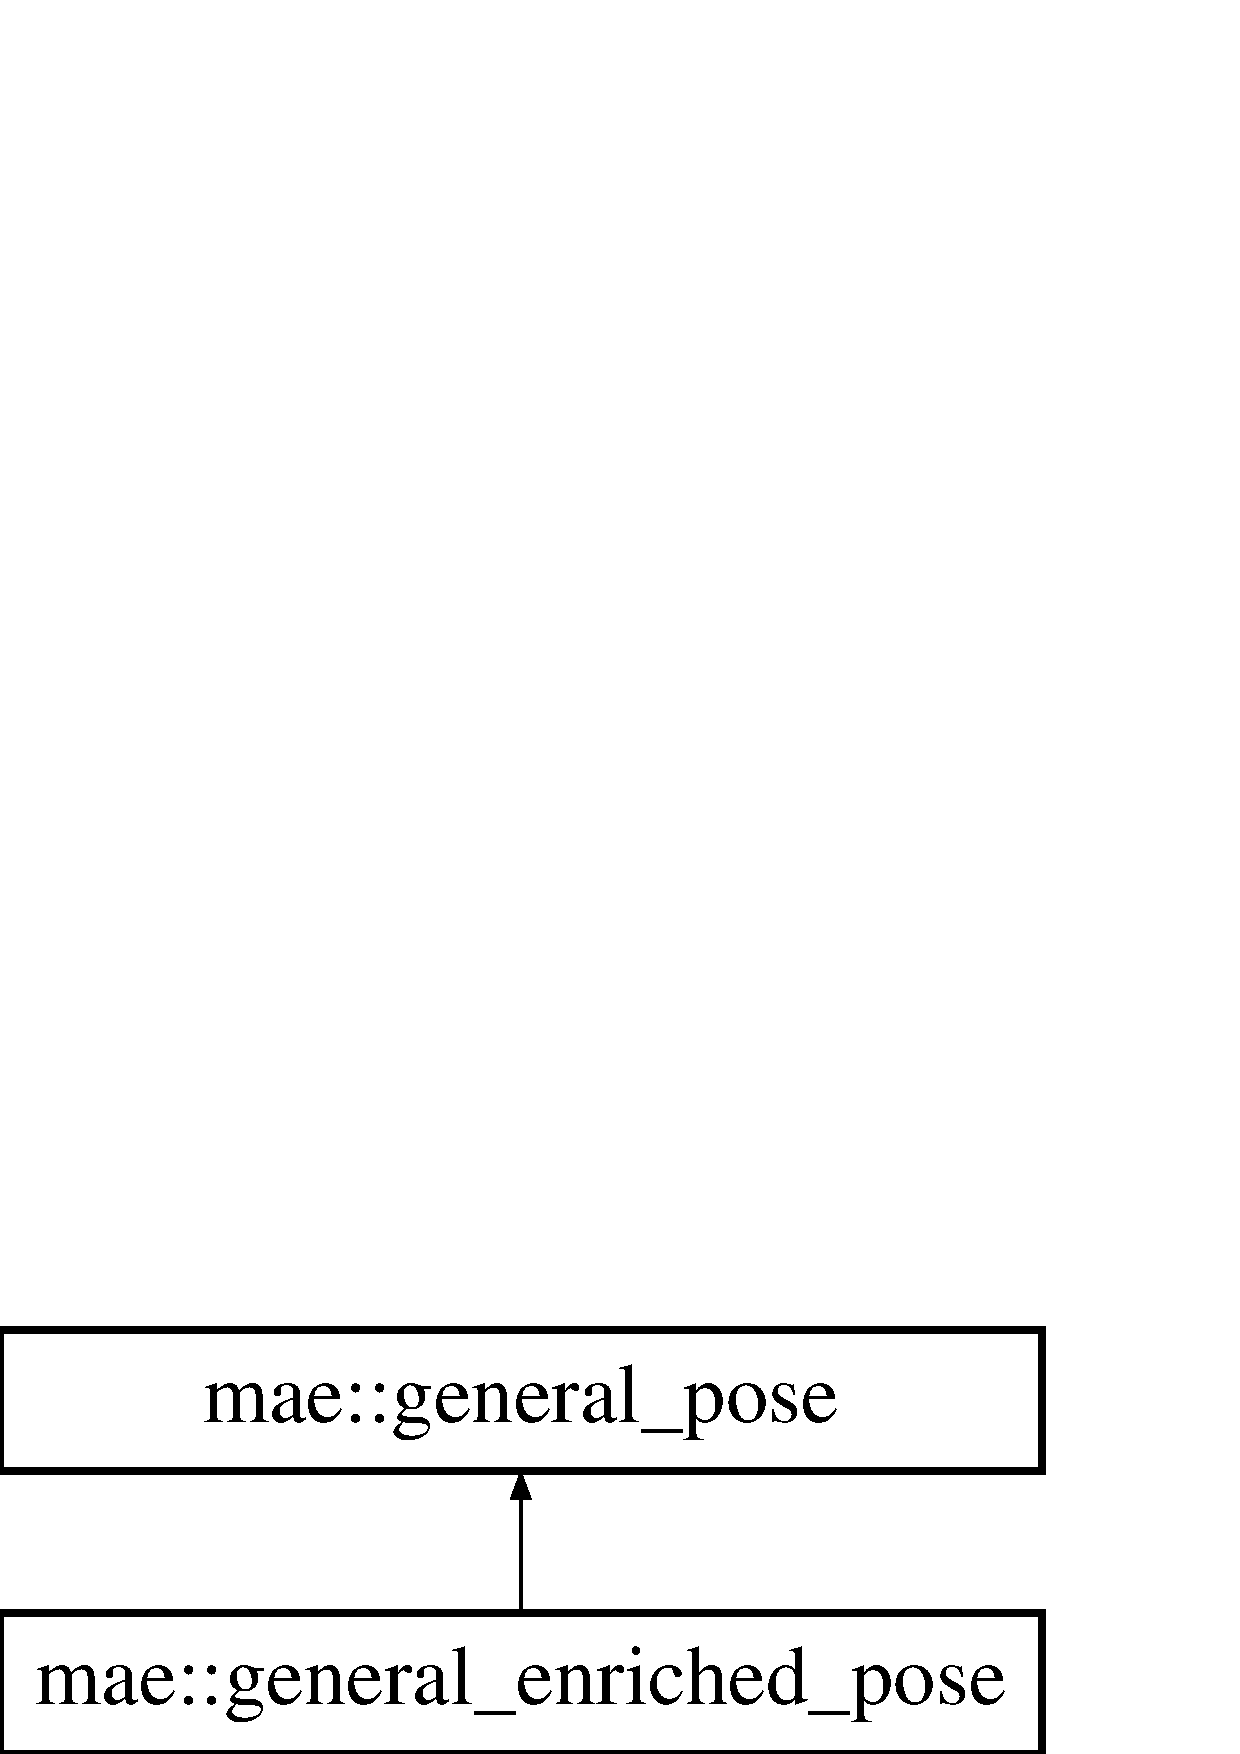
\includegraphics[height=2.000000cm]{classmae_1_1general__pose}
\end{center}
\end{figure}
\subsection*{Public Member Functions}
\begin{DoxyCompactItemize}
\item 
\hyperlink{classmae_1_1general__pose_a62934816ae69c70ff428a9e387944fa3}{general\-\_\-pose} ()
\item 
virtual void \hyperlink{classmae_1_1general__pose_a8dccd4cce6e26b43945230ea3fef9b4e}{set\-\_\-direction} (int body\-\_\-part, int direction)
\item 
virtual int \hyperlink{classmae_1_1general__pose_abdd09dcb3a8fd89c814eab2434ac0420}{get\-\_\-direction} (int body\-\_\-part) const 
\item 
virtual void \hyperlink{classmae_1_1general__pose_a3167544d3cf9dbd740e001c4257d917b}{set\-\_\-distance} (int body\-\_\-part, int direction, double distance)
\item 
virtual double \hyperlink{classmae_1_1general__pose_ae057a89df3dac87b46416ac757c5a370}{get\-\_\-distance} (int body\-\_\-part, int direction) const 
\item 
virtual void \hyperlink{classmae_1_1general__pose_aa747f42741ed76afca30a4cd5afb7ad1}{set\-\_\-rotation} (int body\-\_\-part, double rotation)
\item 
virtual double \hyperlink{classmae_1_1general__pose_a28c802e3b1c6932bbe31836684ba0d14}{get\-\_\-rotation} (int body\-\_\-part) const 
\item 
virtual std\-::list$<$ int $>$ \hyperlink{classmae_1_1general__pose_a75701cd408c10156a55878d05bdd4316}{get\-\_\-body\-\_\-parts} () const 
\item 
virtual std\-::list$<$ int $>$ \hyperlink{classmae_1_1general__pose_ab1b7e20ab2498a07858294de4e3eba8b}{get\-\_\-directions} () const 
\end{DoxyCompactItemize}


\subsection{Constructor \& Destructor Documentation}
\hypertarget{classmae_1_1general__pose_a62934816ae69c70ff428a9e387944fa3}{\index{mae\-::general\-\_\-pose@{mae\-::general\-\_\-pose}!general\-\_\-pose@{general\-\_\-pose}}
\index{general\-\_\-pose@{general\-\_\-pose}!mae::general_pose@{mae\-::general\-\_\-pose}}
\subsubsection[{general\-\_\-pose}]{\setlength{\rightskip}{0pt plus 5cm}mae\-::general\-\_\-pose\-::general\-\_\-pose (
\begin{DoxyParamCaption}
{}
\end{DoxyParamCaption}
)}}\label{classmae_1_1general__pose_a62934816ae69c70ff428a9e387944fa3}
Creates a new empty pose. 

\subsection{Member Function Documentation}
\hypertarget{classmae_1_1general__pose_a75701cd408c10156a55878d05bdd4316}{\index{mae\-::general\-\_\-pose@{mae\-::general\-\_\-pose}!get\-\_\-body\-\_\-parts@{get\-\_\-body\-\_\-parts}}
\index{get\-\_\-body\-\_\-parts@{get\-\_\-body\-\_\-parts}!mae::general_pose@{mae\-::general\-\_\-pose}}
\subsubsection[{get\-\_\-body\-\_\-parts}]{\setlength{\rightskip}{0pt plus 5cm}std\-::list$<$ int $>$ mae\-::general\-\_\-pose\-::get\-\_\-body\-\_\-parts (
\begin{DoxyParamCaption}
{}
\end{DoxyParamCaption}
) const\hspace{0.3cm}{\ttfamily [virtual]}}}\label{classmae_1_1general__pose_a75701cd408c10156a55878d05bdd4316}
Returns all body parts that have a direction assigned to it.

\begin{DoxyReturn}{Returns}
All used body parts in this pose. 
\end{DoxyReturn}
\hypertarget{classmae_1_1general__pose_abdd09dcb3a8fd89c814eab2434ac0420}{\index{mae\-::general\-\_\-pose@{mae\-::general\-\_\-pose}!get\-\_\-direction@{get\-\_\-direction}}
\index{get\-\_\-direction@{get\-\_\-direction}!mae::general_pose@{mae\-::general\-\_\-pose}}
\subsubsection[{get\-\_\-direction}]{\setlength{\rightskip}{0pt plus 5cm}int mae\-::general\-\_\-pose\-::get\-\_\-direction (
\begin{DoxyParamCaption}
\item[{int}]{body\-\_\-part}
\end{DoxyParamCaption}
) const\hspace{0.3cm}{\ttfamily [virtual]}}}\label{classmae_1_1general__pose_abdd09dcb3a8fd89c814eab2434ac0420}
Returns the direction assigned to the body part with the id. If the body part is not listed in this pose zero will be returned indicating an invalid direction.

See fl/fld.\-hpp for laban direction codes used by the fl\-\_\-movement\-\_\-controller.


\begin{DoxyParams}{Parameters}
{\em body\-\_\-part} & The id of the body part (e.\-g. for the left forearm). \\
\hline
\end{DoxyParams}
\begin{DoxyReturn}{Returns}
The direction code. 
\end{DoxyReturn}
\hypertarget{classmae_1_1general__pose_ab1b7e20ab2498a07858294de4e3eba8b}{\index{mae\-::general\-\_\-pose@{mae\-::general\-\_\-pose}!get\-\_\-directions@{get\-\_\-directions}}
\index{get\-\_\-directions@{get\-\_\-directions}!mae::general_pose@{mae\-::general\-\_\-pose}}
\subsubsection[{get\-\_\-directions}]{\setlength{\rightskip}{0pt plus 5cm}std\-::list$<$ int $>$ mae\-::general\-\_\-pose\-::get\-\_\-directions (
\begin{DoxyParamCaption}
{}
\end{DoxyParamCaption}
) const\hspace{0.3cm}{\ttfamily [virtual]}}}\label{classmae_1_1general__pose_ab1b7e20ab2498a07858294de4e3eba8b}
Returns all directions that have a distance assigned.

\begin{DoxyReturn}{Returns}
All directions. 
\end{DoxyReturn}
\hypertarget{classmae_1_1general__pose_ae057a89df3dac87b46416ac757c5a370}{\index{mae\-::general\-\_\-pose@{mae\-::general\-\_\-pose}!get\-\_\-distance@{get\-\_\-distance}}
\index{get\-\_\-distance@{get\-\_\-distance}!mae::general_pose@{mae\-::general\-\_\-pose}}
\subsubsection[{get\-\_\-distance}]{\setlength{\rightskip}{0pt plus 5cm}double mae\-::general\-\_\-pose\-::get\-\_\-distance (
\begin{DoxyParamCaption}
\item[{int}]{body\-\_\-part, }
\item[{int}]{direction}
\end{DoxyParamCaption}
) const\hspace{0.3cm}{\ttfamily [virtual]}}}\label{classmae_1_1general__pose_ae057a89df3dac87b46416ac757c5a370}
Returns the distance of the actual pose to the requested direction for the specific body part. Returns -\/1 if the distance is invalid.

See fl/fld.\-hpp for laban direction codes used by the fl\-\_\-movement\-\_\-controller.


\begin{DoxyParams}{Parameters}
{\em body\-\_\-part} & The id of the body part (e.\-g. for the left forearm). \\
\hline
{\em direction} & The direction code. \\
\hline
\end{DoxyParams}
\begin{DoxyReturn}{Returns}
The distance. 
\end{DoxyReturn}
\hypertarget{classmae_1_1general__pose_a28c802e3b1c6932bbe31836684ba0d14}{\index{mae\-::general\-\_\-pose@{mae\-::general\-\_\-pose}!get\-\_\-rotation@{get\-\_\-rotation}}
\index{get\-\_\-rotation@{get\-\_\-rotation}!mae::general_pose@{mae\-::general\-\_\-pose}}
\subsubsection[{get\-\_\-rotation}]{\setlength{\rightskip}{0pt plus 5cm}double mae\-::general\-\_\-pose\-::get\-\_\-rotation (
\begin{DoxyParamCaption}
\item[{int}]{body\-\_\-part}
\end{DoxyParamCaption}
) const\hspace{0.3cm}{\ttfamily [virtual]}}}\label{classmae_1_1general__pose_a28c802e3b1c6932bbe31836684ba0d14}
Returns the rotation of the body part in the specific pose.


\begin{DoxyParams}{Parameters}
{\em body\-\_\-part} & The body part. \\
\hline
\end{DoxyParams}
\begin{DoxyReturn}{Returns}
The rotation. 
\end{DoxyReturn}
\hypertarget{classmae_1_1general__pose_a8dccd4cce6e26b43945230ea3fef9b4e}{\index{mae\-::general\-\_\-pose@{mae\-::general\-\_\-pose}!set\-\_\-direction@{set\-\_\-direction}}
\index{set\-\_\-direction@{set\-\_\-direction}!mae::general_pose@{mae\-::general\-\_\-pose}}
\subsubsection[{set\-\_\-direction}]{\setlength{\rightskip}{0pt plus 5cm}void mae\-::general\-\_\-pose\-::set\-\_\-direction (
\begin{DoxyParamCaption}
\item[{int}]{body\-\_\-part, }
\item[{int}]{direction}
\end{DoxyParamCaption}
)\hspace{0.3cm}{\ttfamily [virtual]}}}\label{classmae_1_1general__pose_a8dccd4cce6e26b43945230ea3fef9b4e}
Sets the direction for the given body part. The direction should not be zero unless the direction of the body part is meant to be invalidated.

See fl/fld.\-hpp for laban direction codes used by the fl\-\_\-movement\-\_\-controller.


\begin{DoxyParams}{Parameters}
{\em body\-\_\-part} & The id of the body part (e.\-g. for the left forearm). \\
\hline
{\em direction} & The direction code. \\
\hline
\end{DoxyParams}
\hypertarget{classmae_1_1general__pose_a3167544d3cf9dbd740e001c4257d917b}{\index{mae\-::general\-\_\-pose@{mae\-::general\-\_\-pose}!set\-\_\-distance@{set\-\_\-distance}}
\index{set\-\_\-distance@{set\-\_\-distance}!mae::general_pose@{mae\-::general\-\_\-pose}}
\subsubsection[{set\-\_\-distance}]{\setlength{\rightskip}{0pt plus 5cm}void mae\-::general\-\_\-pose\-::set\-\_\-distance (
\begin{DoxyParamCaption}
\item[{int}]{body\-\_\-part, }
\item[{int}]{direction, }
\item[{double}]{distance}
\end{DoxyParamCaption}
)\hspace{0.3cm}{\ttfamily [virtual]}}}\label{classmae_1_1general__pose_a3167544d3cf9dbd740e001c4257d917b}
Sets the distance of a body part to a certain direction. These distances can be used to identify the beginning of a motion from one direction to another. The distance should be positive since -\/1 is used to indicate invalid distances.

See fl/fld.\-hpp for laban direction codes used by the fl\-\_\-movement\-\_\-controller.


\begin{DoxyParams}{Parameters}
{\em body\-\_\-part} & The id of the body part (e.\-g. for the left forearm). \\
\hline
{\em direction} & The direction code. \\
\hline
{\em distance} & The distance. \\
\hline
\end{DoxyParams}
\hypertarget{classmae_1_1general__pose_aa747f42741ed76afca30a4cd5afb7ad1}{\index{mae\-::general\-\_\-pose@{mae\-::general\-\_\-pose}!set\-\_\-rotation@{set\-\_\-rotation}}
\index{set\-\_\-rotation@{set\-\_\-rotation}!mae::general_pose@{mae\-::general\-\_\-pose}}
\subsubsection[{set\-\_\-rotation}]{\setlength{\rightskip}{0pt plus 5cm}void mae\-::general\-\_\-pose\-::set\-\_\-rotation (
\begin{DoxyParamCaption}
\item[{int}]{body\-\_\-part, }
\item[{double}]{rotation}
\end{DoxyParamCaption}
)\hspace{0.3cm}{\ttfamily [virtual]}}}\label{classmae_1_1general__pose_aa747f42741ed76afca30a4cd5afb7ad1}
Sets the rotation of the body part in the specific pose.


\begin{DoxyParams}{Parameters}
{\em body\-\_\-part} & The body part. \\
\hline
{\em rotation} & The rotation. \\
\hline
\end{DoxyParams}


The documentation for this class was generated from the following files\-:\begin{DoxyCompactItemize}
\item 
src/mae/general\-\_\-pose.\-hpp\item 
src/mae/general\-\_\-pose.\-cpp\end{DoxyCompactItemize}

\hypertarget{classmae_1_1general__skeleton}{\section{mae\-:\-:general\-\_\-skeleton Class Reference}
\label{classmae_1_1general__skeleton}\index{mae\-::general\-\_\-skeleton@{mae\-::general\-\_\-skeleton}}
}
Inheritance diagram for mae\-:\-:general\-\_\-skeleton\-:\begin{figure}[H]
\begin{center}
\leavevmode
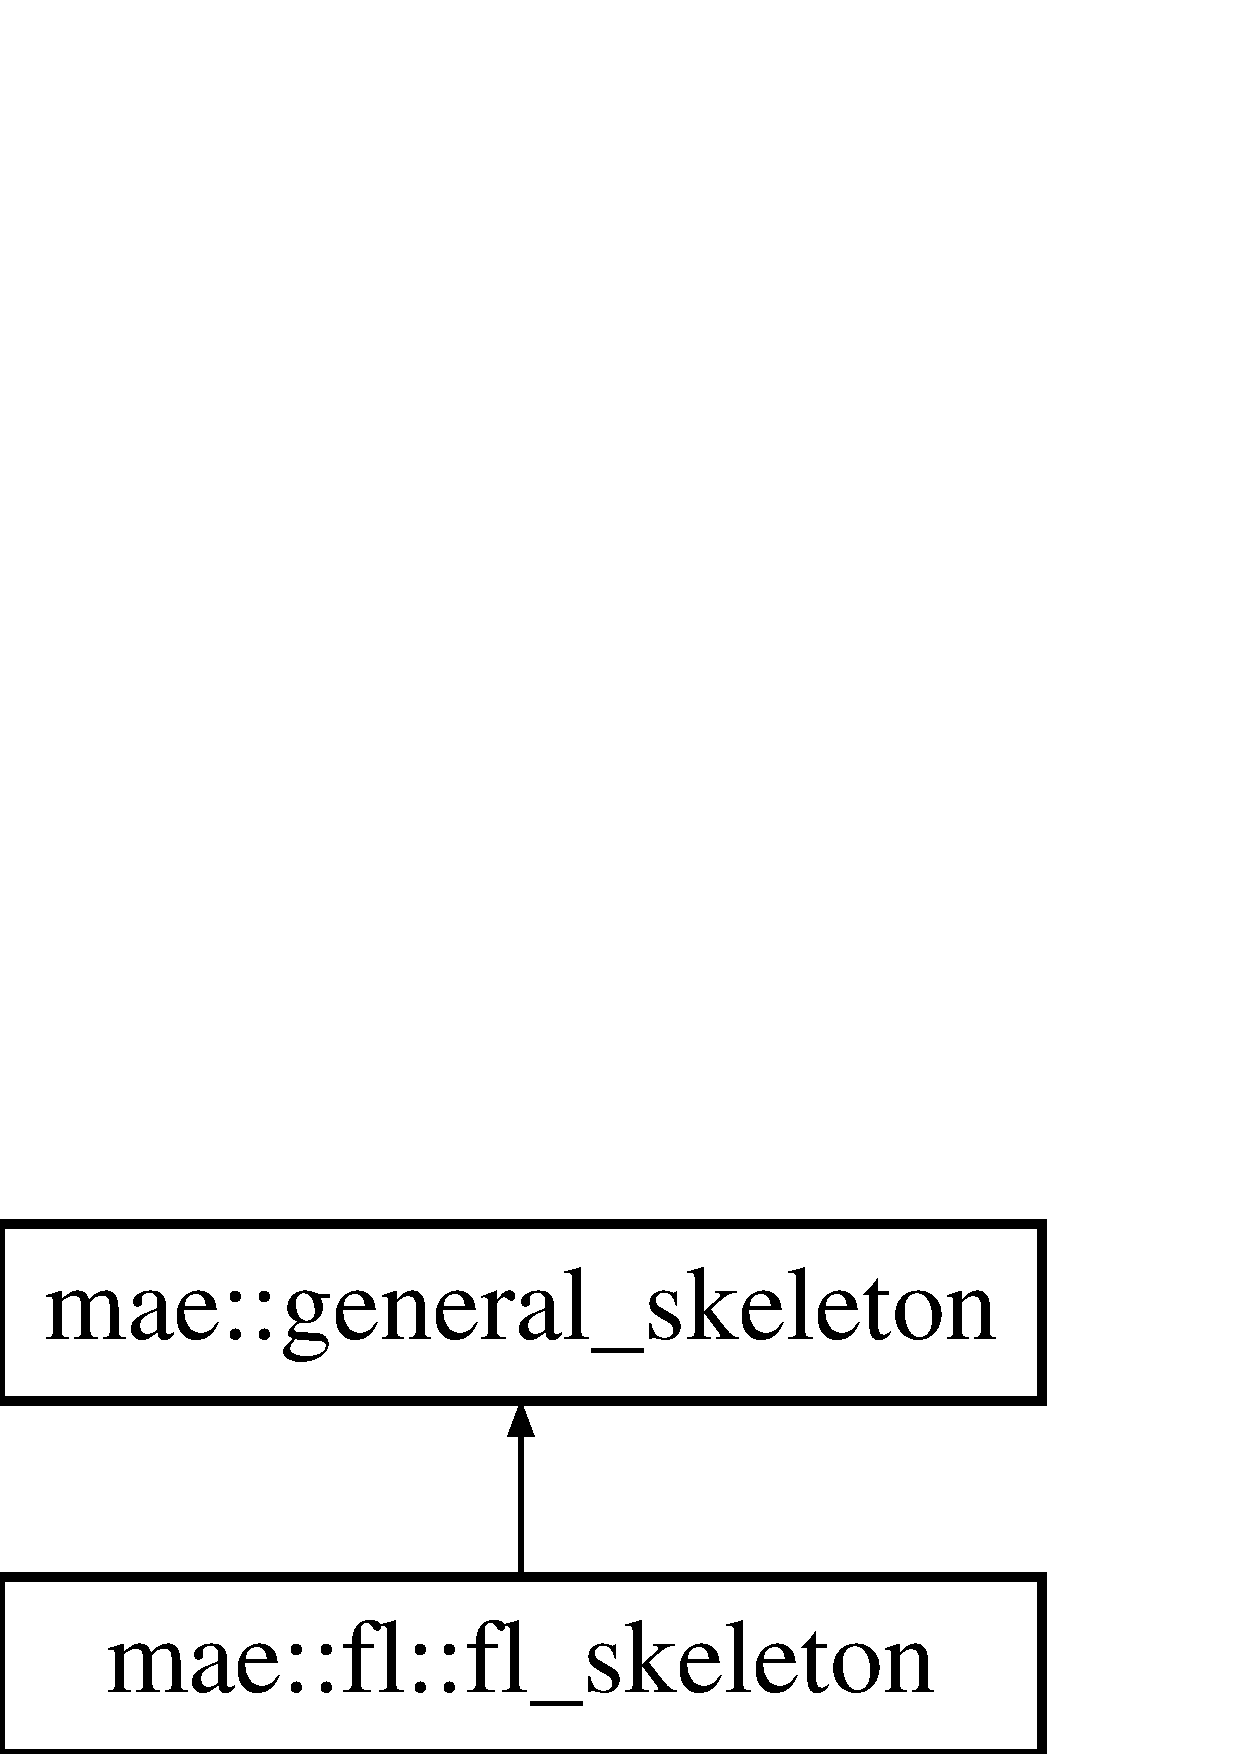
\includegraphics[height=2.000000cm]{classmae_1_1general__skeleton}
\end{center}
\end{figure}
\subsection*{Public Member Functions}
\begin{DoxyCompactItemize}
\item 
\hyperlink{classmae_1_1general__skeleton_a6fef617f6710635df357165f078b9c6f}{general\-\_\-skeleton} ()
\item 
\hyperlink{classmae_1_1general__skeleton_aa79f51739316055ff532e166efcd5055}{general\-\_\-skeleton} (std\-::shared\-\_\-ptr$<$ \hyperlink{classmae_1_1hierarchy}{hierarchy} $>$ \hyperlink{classmae_1_1hierarchy}{hierarchy})
\item 
virtual void \hyperlink{classmae_1_1general__skeleton_ac87486223ea33015136459e8d639c60f}{set\-\_\-joint} (int body\-\_\-part, std\-::shared\-\_\-ptr$<$ \hyperlink{classmae_1_1general__joint}{general\-\_\-joint} $>$ joint)
\item 
virtual std\-::shared\-\_\-ptr\\*
$<$ \hyperlink{classmae_1_1general__joint}{general\-\_\-joint} $>$ \hyperlink{classmae_1_1general__skeleton_a0fd825eaa52585b34d815ef67886b9eb}{get\-\_\-joint} (int body\-\_\-part) const 
\item 
virtual std\-::shared\-\_\-ptr\\*
$<$ \hyperlink{classmae_1_1hierarchy}{hierarchy} $>$ \hyperlink{classmae_1_1general__skeleton_a5455c3c36330399c724f36c477b70d06}{get\-\_\-hierarchy} () const 
\item 
virtual void \hyperlink{classmae_1_1general__skeleton_a3afe48d53ddf26630079ea414e7c953d}{set\-\_\-hierarchy} (std\-::shared\-\_\-ptr$<$ \hyperlink{classmae_1_1hierarchy}{hierarchy} $>$ \hyperlink{classmae_1_1hierarchy}{hierarchy})
\item 
virtual void \hyperlink{classmae_1_1general__skeleton_a9ff97c8b4e17d3dbe881b41485f225f7}{set\-\_\-top\-\_\-down} (std\-::shared\-\_\-ptr$<$ \hyperlink{classmae_1_1bone}{bone} $>$ top\-\_\-down)
\item 
virtual std\-::shared\-\_\-ptr$<$ \hyperlink{classmae_1_1bone}{bone} $>$ \hyperlink{classmae_1_1general__skeleton_a22e697fbaf293090c2a6802fbe803267}{get\-\_\-top\-\_\-down} () const 
\item 
virtual void \hyperlink{classmae_1_1general__skeleton_a276bc0e7dfdb7264bee13e90d9110d3c}{set\-\_\-right\-\_\-left} (std\-::shared\-\_\-ptr$<$ \hyperlink{classmae_1_1bone}{bone} $>$ right\-\_\-left)
\item 
virtual std\-::shared\-\_\-ptr$<$ \hyperlink{classmae_1_1bone}{bone} $>$ \hyperlink{classmae_1_1general__skeleton_a8e85feea644414851d7190e46ef84f13}{get\-\_\-right\-\_\-left} () const 
\item 
virtual void \hyperlink{classmae_1_1general__skeleton_a7f13169da11fac4094b2f829a1c4bd41}{set\-\_\-weight} (std\-::shared\-\_\-ptr$<$ \hyperlink{classmae_1_1math_1_1vec3d}{mae\-::math\-::vec3d} $>$ weight)
\item 
virtual std\-::shared\-\_\-ptr\\*
$<$ \hyperlink{classmae_1_1math_1_1vec3d}{mae\-::math\-::vec3d} $>$ \hyperlink{classmae_1_1general__skeleton_a39ee9e8e865a3d6c4046eb9dd9871e02}{get\-\_\-weight} () const 
\item 
virtual std\-::string \hyperlink{classmae_1_1general__skeleton_a583f49cd26231afbaf9e45decd593f11}{str} () const 
\item 
virtual std\-::string \hyperlink{classmae_1_1general__skeleton_af5305876af2f48217dab7c1e3efc1446}{ply\-\_\-str} () const 
\item 
virtual void \hyperlink{classmae_1_1general__skeleton_a3df84cb9d71969f1a365da48dbebd51f}{ply\-\_\-file} (std\-::string filename) const 
\end{DoxyCompactItemize}
\subsection*{Friends}
\begin{DoxyCompactItemize}
\item 
std\-::ostream \& \hyperlink{classmae_1_1general__skeleton_a05ac4e64849d3f39d1d7613d2b93ccf9}{operator$<$$<$} (std\-::ostream \&os, const std\-::shared\-\_\-ptr$<$ \hyperlink{classmae_1_1general__skeleton}{general\-\_\-skeleton} $>$ \&obj)
\item 
std\-::ostream \& \hyperlink{classmae_1_1general__skeleton_a521f80ff2c6d04d0e8b08e03b7e0a31d}{operator$<$$<$} (std\-::ostream \&os, const \hyperlink{classmae_1_1general__skeleton}{general\-\_\-skeleton} \&obj)
\end{DoxyCompactItemize}


\subsection{Constructor \& Destructor Documentation}
\hypertarget{classmae_1_1general__skeleton_a6fef617f6710635df357165f078b9c6f}{\index{mae\-::general\-\_\-skeleton@{mae\-::general\-\_\-skeleton}!general\-\_\-skeleton@{general\-\_\-skeleton}}
\index{general\-\_\-skeleton@{general\-\_\-skeleton}!mae::general_skeleton@{mae\-::general\-\_\-skeleton}}
\subsubsection[{general\-\_\-skeleton}]{\setlength{\rightskip}{0pt plus 5cm}mae\-::general\-\_\-skeleton\-::general\-\_\-skeleton (
\begin{DoxyParamCaption}
{}
\end{DoxyParamCaption}
)}}\label{classmae_1_1general__skeleton_a6fef617f6710635df357165f078b9c6f}
Creates a general skeleton. \hypertarget{classmae_1_1general__skeleton_aa79f51739316055ff532e166efcd5055}{\index{mae\-::general\-\_\-skeleton@{mae\-::general\-\_\-skeleton}!general\-\_\-skeleton@{general\-\_\-skeleton}}
\index{general\-\_\-skeleton@{general\-\_\-skeleton}!mae::general_skeleton@{mae\-::general\-\_\-skeleton}}
\subsubsection[{general\-\_\-skeleton}]{\setlength{\rightskip}{0pt plus 5cm}mae\-::general\-\_\-skeleton\-::general\-\_\-skeleton (
\begin{DoxyParamCaption}
\item[{std\-::shared\-\_\-ptr$<$ {\bf hierarchy} $>$}]{hierarchy}
\end{DoxyParamCaption}
)}}\label{classmae_1_1general__skeleton_aa79f51739316055ff532e166efcd5055}
Creates a general skeleton with a pre-\/defined hierarchy.


\begin{DoxyParams}{Parameters}
{\em hierarchy} & The hierarchy. \\
\hline
\end{DoxyParams}


\subsection{Member Function Documentation}
\hypertarget{classmae_1_1general__skeleton_a5455c3c36330399c724f36c477b70d06}{\index{mae\-::general\-\_\-skeleton@{mae\-::general\-\_\-skeleton}!get\-\_\-hierarchy@{get\-\_\-hierarchy}}
\index{get\-\_\-hierarchy@{get\-\_\-hierarchy}!mae::general_skeleton@{mae\-::general\-\_\-skeleton}}
\subsubsection[{get\-\_\-hierarchy}]{\setlength{\rightskip}{0pt plus 5cm}std\-::shared\-\_\-ptr$<$ {\bf hierarchy} $>$ mae\-::general\-\_\-skeleton\-::get\-\_\-hierarchy (
\begin{DoxyParamCaption}
{}
\end{DoxyParamCaption}
) const\hspace{0.3cm}{\ttfamily [virtual]}}}\label{classmae_1_1general__skeleton_a5455c3c36330399c724f36c477b70d06}
Returns a shared pointer to the used hierarchy. If not hierarchy is set, a default hierarchy is assumed. \begin{DoxyReturn}{Returns}
A shared pointer to the hierarchy. 
\end{DoxyReturn}
\hypertarget{classmae_1_1general__skeleton_a0fd825eaa52585b34d815ef67886b9eb}{\index{mae\-::general\-\_\-skeleton@{mae\-::general\-\_\-skeleton}!get\-\_\-joint@{get\-\_\-joint}}
\index{get\-\_\-joint@{get\-\_\-joint}!mae::general_skeleton@{mae\-::general\-\_\-skeleton}}
\subsubsection[{get\-\_\-joint}]{\setlength{\rightskip}{0pt plus 5cm}std\-::shared\-\_\-ptr$<$ {\bf general\-\_\-joint} $>$ mae\-::general\-\_\-skeleton\-::get\-\_\-joint (
\begin{DoxyParamCaption}
\item[{int}]{body\-\_\-part}
\end{DoxyParamCaption}
) const\hspace{0.3cm}{\ttfamily [virtual]}}}\label{classmae_1_1general__skeleton_a0fd825eaa52585b34d815ef67886b9eb}
Returns a shared pointer to the joint of the body part.


\begin{DoxyParams}{Parameters}
{\em body\-Part} & The addressed body part. \\
\hline
\end{DoxyParams}
\begin{DoxyReturn}{Returns}
A shared pointer to the joint. 
\end{DoxyReturn}
\hypertarget{classmae_1_1general__skeleton_a8e85feea644414851d7190e46ef84f13}{\index{mae\-::general\-\_\-skeleton@{mae\-::general\-\_\-skeleton}!get\-\_\-right\-\_\-left@{get\-\_\-right\-\_\-left}}
\index{get\-\_\-right\-\_\-left@{get\-\_\-right\-\_\-left}!mae::general_skeleton@{mae\-::general\-\_\-skeleton}}
\subsubsection[{get\-\_\-right\-\_\-left}]{\setlength{\rightskip}{0pt plus 5cm}std\-::shared\-\_\-ptr$<$ {\bf bone} $>$ mae\-::general\-\_\-skeleton\-::get\-\_\-right\-\_\-left (
\begin{DoxyParamCaption}
{}
\end{DoxyParamCaption}
) const\hspace{0.3cm}{\ttfamily [virtual]}}}\label{classmae_1_1general__skeleton_a8e85feea644414851d7190e46ef84f13}
Returns the right-\/left direction of this skeleton by giving a bone. The bone ranges from one torso joint to another.


\begin{DoxyParams}{Parameters}
{\em top\-\_\-down} & A shared pointer to the bone. \\
\hline
\end{DoxyParams}
\hypertarget{classmae_1_1general__skeleton_a22e697fbaf293090c2a6802fbe803267}{\index{mae\-::general\-\_\-skeleton@{mae\-::general\-\_\-skeleton}!get\-\_\-top\-\_\-down@{get\-\_\-top\-\_\-down}}
\index{get\-\_\-top\-\_\-down@{get\-\_\-top\-\_\-down}!mae::general_skeleton@{mae\-::general\-\_\-skeleton}}
\subsubsection[{get\-\_\-top\-\_\-down}]{\setlength{\rightskip}{0pt plus 5cm}std\-::shared\-\_\-ptr$<$ {\bf bone} $>$ mae\-::general\-\_\-skeleton\-::get\-\_\-top\-\_\-down (
\begin{DoxyParamCaption}
{}
\end{DoxyParamCaption}
) const\hspace{0.3cm}{\ttfamily [virtual]}}}\label{classmae_1_1general__skeleton_a22e697fbaf293090c2a6802fbe803267}
Returns the top-\/down direction of this skeleton by giving a bone. The bone ranges from one torso joint to another.


\begin{DoxyParams}{Parameters}
{\em top\-\_\-down} & A shared pointer to the bone. \\
\hline
\end{DoxyParams}
\hypertarget{classmae_1_1general__skeleton_a39ee9e8e865a3d6c4046eb9dd9871e02}{\index{mae\-::general\-\_\-skeleton@{mae\-::general\-\_\-skeleton}!get\-\_\-weight@{get\-\_\-weight}}
\index{get\-\_\-weight@{get\-\_\-weight}!mae::general_skeleton@{mae\-::general\-\_\-skeleton}}
\subsubsection[{get\-\_\-weight}]{\setlength{\rightskip}{0pt plus 5cm}std\-::shared\-\_\-ptr$<$ {\bf mae\-::math\-::vec3d} $>$ mae\-::general\-\_\-skeleton\-::get\-\_\-weight (
\begin{DoxyParamCaption}
{}
\end{DoxyParamCaption}
) const\hspace{0.3cm}{\ttfamily [virtual]}}}\label{classmae_1_1general__skeleton_a39ee9e8e865a3d6c4046eb9dd9871e02}
Returns the weight vector for this skeleton. If none is set, a null pointer will be returned.

\begin{DoxyReturn}{Returns}
The weight or null. 
\end{DoxyReturn}
\hypertarget{classmae_1_1general__skeleton_a3df84cb9d71969f1a365da48dbebd51f}{\index{mae\-::general\-\_\-skeleton@{mae\-::general\-\_\-skeleton}!ply\-\_\-file@{ply\-\_\-file}}
\index{ply\-\_\-file@{ply\-\_\-file}!mae::general_skeleton@{mae\-::general\-\_\-skeleton}}
\subsubsection[{ply\-\_\-file}]{\setlength{\rightskip}{0pt plus 5cm}void mae\-::general\-\_\-skeleton\-::ply\-\_\-file (
\begin{DoxyParamCaption}
\item[{std\-::string}]{filename}
\end{DoxyParamCaption}
) const\hspace{0.3cm}{\ttfamily [virtual]}}}\label{classmae_1_1general__skeleton_a3df84cb9d71969f1a365da48dbebd51f}
Exports the skeleton data to the file using the Stanford Triangle Format format.


\begin{DoxyParams}{Parameters}
{\em filename} & The target output file. \\
\hline
\end{DoxyParams}
\hypertarget{classmae_1_1general__skeleton_af5305876af2f48217dab7c1e3efc1446}{\index{mae\-::general\-\_\-skeleton@{mae\-::general\-\_\-skeleton}!ply\-\_\-str@{ply\-\_\-str}}
\index{ply\-\_\-str@{ply\-\_\-str}!mae::general_skeleton@{mae\-::general\-\_\-skeleton}}
\subsubsection[{ply\-\_\-str}]{\setlength{\rightskip}{0pt plus 5cm}std\-::string mae\-::general\-\_\-skeleton\-::ply\-\_\-str (
\begin{DoxyParamCaption}
{}
\end{DoxyParamCaption}
) const\hspace{0.3cm}{\ttfamily [virtual]}}}\label{classmae_1_1general__skeleton_af5305876af2f48217dab7c1e3efc1446}
Exports the skeleton data in the Stanford Triagle format as a string. \begin{DoxyReturn}{Returns}

\end{DoxyReturn}
\hypertarget{classmae_1_1general__skeleton_a3afe48d53ddf26630079ea414e7c953d}{\index{mae\-::general\-\_\-skeleton@{mae\-::general\-\_\-skeleton}!set\-\_\-hierarchy@{set\-\_\-hierarchy}}
\index{set\-\_\-hierarchy@{set\-\_\-hierarchy}!mae::general_skeleton@{mae\-::general\-\_\-skeleton}}
\subsubsection[{set\-\_\-hierarchy}]{\setlength{\rightskip}{0pt plus 5cm}void mae\-::general\-\_\-skeleton\-::set\-\_\-hierarchy (
\begin{DoxyParamCaption}
\item[{std\-::shared\-\_\-ptr$<$ {\bf hierarchy} $>$}]{hierarchy}
\end{DoxyParamCaption}
)\hspace{0.3cm}{\ttfamily [virtual]}}}\label{classmae_1_1general__skeleton_a3afe48d53ddf26630079ea414e7c953d}
Sets the hierarchy 
\begin{DoxyParams}{Parameters}
{\em hierarchy} & A smart pointer to the hierarchy. \\
\hline
\end{DoxyParams}
\hypertarget{classmae_1_1general__skeleton_ac87486223ea33015136459e8d639c60f}{\index{mae\-::general\-\_\-skeleton@{mae\-::general\-\_\-skeleton}!set\-\_\-joint@{set\-\_\-joint}}
\index{set\-\_\-joint@{set\-\_\-joint}!mae::general_skeleton@{mae\-::general\-\_\-skeleton}}
\subsubsection[{set\-\_\-joint}]{\setlength{\rightskip}{0pt plus 5cm}void mae\-::general\-\_\-skeleton\-::set\-\_\-joint (
\begin{DoxyParamCaption}
\item[{int}]{body\-\_\-part, }
\item[{std\-::shared\-\_\-ptr$<$ {\bf general\-\_\-joint} $>$}]{joint}
\end{DoxyParamCaption}
)\hspace{0.3cm}{\ttfamily [virtual]}}}\label{classmae_1_1general__skeleton_ac87486223ea33015136459e8d639c60f}
Sets a new joint for the given body part.


\begin{DoxyParams}{Parameters}
{\em body\-Part} & The addressed body part. \\
\hline
{\em joint} & A shared pointer to the joint. \\
\hline
\end{DoxyParams}
\hypertarget{classmae_1_1general__skeleton_a276bc0e7dfdb7264bee13e90d9110d3c}{\index{mae\-::general\-\_\-skeleton@{mae\-::general\-\_\-skeleton}!set\-\_\-right\-\_\-left@{set\-\_\-right\-\_\-left}}
\index{set\-\_\-right\-\_\-left@{set\-\_\-right\-\_\-left}!mae::general_skeleton@{mae\-::general\-\_\-skeleton}}
\subsubsection[{set\-\_\-right\-\_\-left}]{\setlength{\rightskip}{0pt plus 5cm}void mae\-::general\-\_\-skeleton\-::set\-\_\-right\-\_\-left (
\begin{DoxyParamCaption}
\item[{std\-::shared\-\_\-ptr$<$ {\bf bone} $>$}]{right\-\_\-left}
\end{DoxyParamCaption}
)\hspace{0.3cm}{\ttfamily [virtual]}}}\label{classmae_1_1general__skeleton_a276bc0e7dfdb7264bee13e90d9110d3c}
Sets the right-\/left direction of this skeleton by defining a bone. The bone must range from one torso joint to another and need not to follow the hierarchy (but the id's must be defined).


\begin{DoxyParams}{Parameters}
{\em top\-\_\-down} & A shared pointer to the bone. \\
\hline
\end{DoxyParams}
\hypertarget{classmae_1_1general__skeleton_a9ff97c8b4e17d3dbe881b41485f225f7}{\index{mae\-::general\-\_\-skeleton@{mae\-::general\-\_\-skeleton}!set\-\_\-top\-\_\-down@{set\-\_\-top\-\_\-down}}
\index{set\-\_\-top\-\_\-down@{set\-\_\-top\-\_\-down}!mae::general_skeleton@{mae\-::general\-\_\-skeleton}}
\subsubsection[{set\-\_\-top\-\_\-down}]{\setlength{\rightskip}{0pt plus 5cm}void mae\-::general\-\_\-skeleton\-::set\-\_\-top\-\_\-down (
\begin{DoxyParamCaption}
\item[{std\-::shared\-\_\-ptr$<$ {\bf bone} $>$}]{top\-\_\-down}
\end{DoxyParamCaption}
)\hspace{0.3cm}{\ttfamily [virtual]}}}\label{classmae_1_1general__skeleton_a9ff97c8b4e17d3dbe881b41485f225f7}
Sets the top-\/down direction of this skeleton by defining a bone. The bone must range from one torso joint to another and need not to follow the hierarchy (but the id's must be defined).


\begin{DoxyParams}{Parameters}
{\em top\-\_\-down} & A shared pointer to the bone. \\
\hline
\end{DoxyParams}
\hypertarget{classmae_1_1general__skeleton_a7f13169da11fac4094b2f829a1c4bd41}{\index{mae\-::general\-\_\-skeleton@{mae\-::general\-\_\-skeleton}!set\-\_\-weight@{set\-\_\-weight}}
\index{set\-\_\-weight@{set\-\_\-weight}!mae::general_skeleton@{mae\-::general\-\_\-skeleton}}
\subsubsection[{set\-\_\-weight}]{\setlength{\rightskip}{0pt plus 5cm}void mae\-::general\-\_\-skeleton\-::set\-\_\-weight (
\begin{DoxyParamCaption}
\item[{std\-::shared\-\_\-ptr$<$ {\bf mae\-::math\-::vec3d} $>$}]{weight}
\end{DoxyParamCaption}
)\hspace{0.3cm}{\ttfamily [virtual]}}}\label{classmae_1_1general__skeleton_a7f13169da11fac4094b2f829a1c4bd41}
Sets the weight vector for this skeleton.


\begin{DoxyParams}{Parameters}
{\em weight} & The weight vector. \\
\hline
\end{DoxyParams}
\hypertarget{classmae_1_1general__skeleton_a583f49cd26231afbaf9e45decd593f11}{\index{mae\-::general\-\_\-skeleton@{mae\-::general\-\_\-skeleton}!str@{str}}
\index{str@{str}!mae::general_skeleton@{mae\-::general\-\_\-skeleton}}
\subsubsection[{str}]{\setlength{\rightskip}{0pt plus 5cm}std\-::string mae\-::general\-\_\-skeleton\-::str (
\begin{DoxyParamCaption}
{}
\end{DoxyParamCaption}
) const\hspace{0.3cm}{\ttfamily [virtual]}}}\label{classmae_1_1general__skeleton_a583f49cd26231afbaf9e45decd593f11}
Converts this object to a string.

\begin{DoxyReturn}{Returns}
This object as a string. 
\end{DoxyReturn}


Reimplemented in \hyperlink{classmae_1_1fl_1_1fl__skeleton_ad759f12bd33a9b0fd801eab2018c64de}{mae\-::fl\-::fl\-\_\-skeleton}.



\subsection{Friends And Related Function Documentation}
\hypertarget{classmae_1_1general__skeleton_a05ac4e64849d3f39d1d7613d2b93ccf9}{\index{mae\-::general\-\_\-skeleton@{mae\-::general\-\_\-skeleton}!operator$<$$<$@{operator$<$$<$}}
\index{operator$<$$<$@{operator$<$$<$}!mae::general_skeleton@{mae\-::general\-\_\-skeleton}}
\subsubsection[{operator$<$$<$}]{\setlength{\rightskip}{0pt plus 5cm}std\-::ostream\& operator$<$$<$ (
\begin{DoxyParamCaption}
\item[{std\-::ostream \&}]{os, }
\item[{const std\-::shared\-\_\-ptr$<$ {\bf general\-\_\-skeleton} $>$ \&}]{obj}
\end{DoxyParamCaption}
)\hspace{0.3cm}{\ttfamily [friend]}}}\label{classmae_1_1general__skeleton_a05ac4e64849d3f39d1d7613d2b93ccf9}
Prints the object to the stream.


\begin{DoxyParams}{Parameters}
{\em os} & \\
\hline
{\em obj} & The object to be printed. \\
\hline
\end{DoxyParams}
\begin{DoxyReturn}{Returns}

\end{DoxyReturn}
\hypertarget{classmae_1_1general__skeleton_a521f80ff2c6d04d0e8b08e03b7e0a31d}{\index{mae\-::general\-\_\-skeleton@{mae\-::general\-\_\-skeleton}!operator$<$$<$@{operator$<$$<$}}
\index{operator$<$$<$@{operator$<$$<$}!mae::general_skeleton@{mae\-::general\-\_\-skeleton}}
\subsubsection[{operator$<$$<$}]{\setlength{\rightskip}{0pt plus 5cm}std\-::ostream\& operator$<$$<$ (
\begin{DoxyParamCaption}
\item[{std\-::ostream \&}]{os, }
\item[{const {\bf general\-\_\-skeleton} \&}]{obj}
\end{DoxyParamCaption}
)\hspace{0.3cm}{\ttfamily [friend]}}}\label{classmae_1_1general__skeleton_a521f80ff2c6d04d0e8b08e03b7e0a31d}
Prints the object to the stream.


\begin{DoxyParams}{Parameters}
{\em os} & \\
\hline
{\em obj} & The object to be printed. \\
\hline
\end{DoxyParams}
\begin{DoxyReturn}{Returns}

\end{DoxyReturn}


The documentation for this class was generated from the following files\-:\begin{DoxyCompactItemize}
\item 
src/mae/general\-\_\-skeleton.\-hpp\item 
src/mae/general\-\_\-skeleton.\-cpp\end{DoxyCompactItemize}

\hypertarget{classmae_1_1hierarchy}{\section{mae\-:\-:hierarchy Class Reference}
\label{classmae_1_1hierarchy}\index{mae\-::hierarchy@{mae\-::hierarchy}}
}
\subsection*{Public Member Functions}
\begin{DoxyCompactItemize}
\item 
\hyperlink{classmae_1_1hierarchy_ad8006ba53f5228fa32e5040eba48a2ba}{hierarchy} ()
\item 
\hyperlink{classmae_1_1hierarchy_a078873a827d93987db7b149a698144f7}{hierarchy} (std\-::shared\-\_\-ptr$<$ \hyperlink{classmae_1_1hierarchy__element}{hierarchy\-\_\-element} $>$ root)
\item 
virtual \hyperlink{classmae_1_1hierarchy_a24cca85994f8bac7c078f0f2b63f37cd}{$\sim$hierarchy} ()
\item 
virtual std\-::shared\-\_\-ptr\\*
$<$ \hyperlink{classmae_1_1hierarchy__element}{hierarchy\-\_\-element} $>$ \hyperlink{classmae_1_1hierarchy_a67f50abac7cdceff6b2d4a2e5db80e1c}{get\-\_\-root} () const 
\item 
virtual void \hyperlink{classmae_1_1hierarchy_ab4f151f5e91d7078d41e9b0d65ea88df}{set\-\_\-root} (std\-::shared\-\_\-ptr$<$ \hyperlink{classmae_1_1hierarchy__element}{hierarchy\-\_\-element} $>$ root)
\item 
virtual std\-::vector\\*
$<$ std\-::shared\-\_\-ptr\\*
$<$ \hyperlink{classmae_1_1hierarchy__element}{hierarchy\-\_\-element} $>$ $>$ \hyperlink{classmae_1_1hierarchy_a1f7df9e7e9d86e24a62359da3b8a72fe}{get\-\_\-element\-\_\-sequence} ()
\item 
virtual \hyperlink{classmae_1_1hierarchy__element}{hierarchy\-\_\-element} $\ast$const \hyperlink{classmae_1_1hierarchy_abc29a6cb37845624d40680f1c01ebd96}{at} (int element\-\_\-id) const 
\item 
virtual std\-::string \hyperlink{classmae_1_1hierarchy_a09756b507aa2fefb8e54f854333aa93d}{str} () const 
\end{DoxyCompactItemize}
\subsection*{Static Public Member Functions}
\begin{DoxyCompactItemize}
\item 
static std\-::shared\-\_\-ptr$<$ \hyperlink{classmae_1_1hierarchy}{hierarchy} $>$ \hyperlink{classmae_1_1hierarchy_a2d5a7b8af3c883a113bd3bf8756181e0}{default\-\_\-hierarchy} ()
\end{DoxyCompactItemize}
\subsection*{Protected Member Functions}
\begin{DoxyCompactItemize}
\item 
virtual void \hyperlink{classmae_1_1hierarchy_ae883a463039fe4fbcaa660e44e25c476}{add\-\_\-element} (\hyperlink{classmae_1_1hierarchy__element}{hierarchy\-\_\-element} $\ast$const element)
\item 
virtual void \hyperlink{classmae_1_1hierarchy_a430b470b34db741bb22552d2a534c733}{remove\-\_\-element} (\hyperlink{classmae_1_1hierarchy__element}{hierarchy\-\_\-element} $\ast$const element)
\end{DoxyCompactItemize}
\subsection*{Friends}
\begin{DoxyCompactItemize}
\item 
\hypertarget{classmae_1_1hierarchy_a7ef536ecd89121e2f44377643ceda64e}{class {\bfseries hierarchy\-\_\-element}}\label{classmae_1_1hierarchy_a7ef536ecd89121e2f44377643ceda64e}

\end{DoxyCompactItemize}


\subsection{Constructor \& Destructor Documentation}
\hypertarget{classmae_1_1hierarchy_ad8006ba53f5228fa32e5040eba48a2ba}{\index{mae\-::hierarchy@{mae\-::hierarchy}!hierarchy@{hierarchy}}
\index{hierarchy@{hierarchy}!mae::hierarchy@{mae\-::hierarchy}}
\subsubsection[{hierarchy}]{\setlength{\rightskip}{0pt plus 5cm}mae\-::hierarchy\-::hierarchy (
\begin{DoxyParamCaption}
{}
\end{DoxyParamCaption}
)}}\label{classmae_1_1hierarchy_ad8006ba53f5228fa32e5040eba48a2ba}
Creates a new empty hierarchy. \hypertarget{classmae_1_1hierarchy_a078873a827d93987db7b149a698144f7}{\index{mae\-::hierarchy@{mae\-::hierarchy}!hierarchy@{hierarchy}}
\index{hierarchy@{hierarchy}!mae::hierarchy@{mae\-::hierarchy}}
\subsubsection[{hierarchy}]{\setlength{\rightskip}{0pt plus 5cm}mae\-::hierarchy\-::hierarchy (
\begin{DoxyParamCaption}
\item[{std\-::shared\-\_\-ptr$<$ {\bf hierarchy\-\_\-element} $>$}]{root}
\end{DoxyParamCaption}
)}}\label{classmae_1_1hierarchy_a078873a827d93987db7b149a698144f7}
Creates a new hierarchy giving the root of elements.


\begin{DoxyParams}{Parameters}
{\em root} & The root which is (in-\/)direct parent of all elements. \\
\hline
\end{DoxyParams}
\hypertarget{classmae_1_1hierarchy_a24cca85994f8bac7c078f0f2b63f37cd}{\index{mae\-::hierarchy@{mae\-::hierarchy}!$\sim$hierarchy@{$\sim$hierarchy}}
\index{$\sim$hierarchy@{$\sim$hierarchy}!mae::hierarchy@{mae\-::hierarchy}}
\subsubsection[{$\sim$hierarchy}]{\setlength{\rightskip}{0pt plus 5cm}mae\-::hierarchy\-::$\sim$hierarchy (
\begin{DoxyParamCaption}
{}
\end{DoxyParamCaption}
)\hspace{0.3cm}{\ttfamily [virtual]}}}\label{classmae_1_1hierarchy_a24cca85994f8bac7c078f0f2b63f37cd}
Destructs this element and fixes the root (hierarchy). 

\subsection{Member Function Documentation}
\hypertarget{classmae_1_1hierarchy_ae883a463039fe4fbcaa660e44e25c476}{\index{mae\-::hierarchy@{mae\-::hierarchy}!add\-\_\-element@{add\-\_\-element}}
\index{add\-\_\-element@{add\-\_\-element}!mae::hierarchy@{mae\-::hierarchy}}
\subsubsection[{add\-\_\-element}]{\setlength{\rightskip}{0pt plus 5cm}void mae\-::hierarchy\-::add\-\_\-element (
\begin{DoxyParamCaption}
\item[{{\bf hierarchy\-\_\-element} $\ast$const}]{element}
\end{DoxyParamCaption}
)\hspace{0.3cm}{\ttfamily [protected]}, {\ttfamily [virtual]}}}\label{classmae_1_1hierarchy_ae883a463039fe4fbcaa660e44e25c476}
Adds a new element to the elements hashmap in order to provide fast access to the elements. This method is invoked automatically from the Hierarchy\-Element.


\begin{DoxyParams}{Parameters}
{\em element} & The element to be added. \\
\hline
\end{DoxyParams}
\hypertarget{classmae_1_1hierarchy_abc29a6cb37845624d40680f1c01ebd96}{\index{mae\-::hierarchy@{mae\-::hierarchy}!at@{at}}
\index{at@{at}!mae::hierarchy@{mae\-::hierarchy}}
\subsubsection[{at}]{\setlength{\rightskip}{0pt plus 5cm}{\bf hierarchy\-\_\-element} $\ast$const mae\-::hierarchy\-::at (
\begin{DoxyParamCaption}
\item[{int}]{element\-\_\-id}
\end{DoxyParamCaption}
) const\hspace{0.3cm}{\ttfamily [virtual]}}}\label{classmae_1_1hierarchy_abc29a6cb37845624d40680f1c01ebd96}
Returns the element with the given id. This is done in constant time.


\begin{DoxyParams}{Parameters}
{\em element\-\_\-id} & The element's id. \\
\hline
\end{DoxyParams}
\begin{DoxyReturn}{Returns}
A plain pointer to the element. 
\end{DoxyReturn}
\hypertarget{classmae_1_1hierarchy_a2d5a7b8af3c883a113bd3bf8756181e0}{\index{mae\-::hierarchy@{mae\-::hierarchy}!default\-\_\-hierarchy@{default\-\_\-hierarchy}}
\index{default\-\_\-hierarchy@{default\-\_\-hierarchy}!mae::hierarchy@{mae\-::hierarchy}}
\subsubsection[{default\-\_\-hierarchy}]{\setlength{\rightskip}{0pt plus 5cm}std\-::shared\-\_\-ptr$<$ {\bf hierarchy} $>$ mae\-::hierarchy\-::default\-\_\-hierarchy (
\begin{DoxyParamCaption}
{}
\end{DoxyParamCaption}
)\hspace{0.3cm}{\ttfamily [static]}}}\label{classmae_1_1hierarchy_a2d5a7b8af3c883a113bd3bf8756181e0}
Returns a default hierarchy that fits the needs of the Open\-N\-I/\-Ni\-T\-E skeletons. If the Open\-N\-I/\-Ni\-T\-E hierarchy is not sufficient and/or another hierarchy is needed it must be constructed manually.

\begin{DoxyReturn}{Returns}
The default hierarchy. 
\end{DoxyReturn}
\hypertarget{classmae_1_1hierarchy_a1f7df9e7e9d86e24a62359da3b8a72fe}{\index{mae\-::hierarchy@{mae\-::hierarchy}!get\-\_\-element\-\_\-sequence@{get\-\_\-element\-\_\-sequence}}
\index{get\-\_\-element\-\_\-sequence@{get\-\_\-element\-\_\-sequence}!mae::hierarchy@{mae\-::hierarchy}}
\subsubsection[{get\-\_\-element\-\_\-sequence}]{\setlength{\rightskip}{0pt plus 5cm}std\-::vector$<$ std\-::shared\-\_\-ptr$<$ {\bf hierarchy\-\_\-element} $>$ $>$ mae\-::hierarchy\-::get\-\_\-element\-\_\-sequence (
\begin{DoxyParamCaption}
{}
\end{DoxyParamCaption}
)\hspace{0.3cm}{\ttfamily [virtual]}}}\label{classmae_1_1hierarchy_a1f7df9e7e9d86e24a62359da3b8a72fe}
Returns the element sequence containing all elements of this hierarchy.

\begin{DoxyReturn}{Returns}
The sequence. 
\end{DoxyReturn}
\hypertarget{classmae_1_1hierarchy_a67f50abac7cdceff6b2d4a2e5db80e1c}{\index{mae\-::hierarchy@{mae\-::hierarchy}!get\-\_\-root@{get\-\_\-root}}
\index{get\-\_\-root@{get\-\_\-root}!mae::hierarchy@{mae\-::hierarchy}}
\subsubsection[{get\-\_\-root}]{\setlength{\rightskip}{0pt plus 5cm}std\-::shared\-\_\-ptr$<$ {\bf hierarchy\-\_\-element} $>$ mae\-::hierarchy\-::get\-\_\-root (
\begin{DoxyParamCaption}
{}
\end{DoxyParamCaption}
) const\hspace{0.3cm}{\ttfamily [virtual]}}}\label{classmae_1_1hierarchy_a67f50abac7cdceff6b2d4a2e5db80e1c}
Returns a shared pointer to the root element.

\begin{DoxyReturn}{Returns}
The root element. 
\end{DoxyReturn}
\hypertarget{classmae_1_1hierarchy_a430b470b34db741bb22552d2a534c733}{\index{mae\-::hierarchy@{mae\-::hierarchy}!remove\-\_\-element@{remove\-\_\-element}}
\index{remove\-\_\-element@{remove\-\_\-element}!mae::hierarchy@{mae\-::hierarchy}}
\subsubsection[{remove\-\_\-element}]{\setlength{\rightskip}{0pt plus 5cm}void mae\-::hierarchy\-::remove\-\_\-element (
\begin{DoxyParamCaption}
\item[{{\bf hierarchy\-\_\-element} $\ast$const}]{element}
\end{DoxyParamCaption}
)\hspace{0.3cm}{\ttfamily [protected]}, {\ttfamily [virtual]}}}\label{classmae_1_1hierarchy_a430b470b34db741bb22552d2a534c733}
Removes an element from the elements hashmap in order to provide fast access to the elements. This method is invoked automatically from the Hierarchy\-Element.


\begin{DoxyParams}{Parameters}
{\em element} & The element to be removed \\
\hline
\end{DoxyParams}
\hypertarget{classmae_1_1hierarchy_ab4f151f5e91d7078d41e9b0d65ea88df}{\index{mae\-::hierarchy@{mae\-::hierarchy}!set\-\_\-root@{set\-\_\-root}}
\index{set\-\_\-root@{set\-\_\-root}!mae::hierarchy@{mae\-::hierarchy}}
\subsubsection[{set\-\_\-root}]{\setlength{\rightskip}{0pt plus 5cm}void mae\-::hierarchy\-::set\-\_\-root (
\begin{DoxyParamCaption}
\item[{std\-::shared\-\_\-ptr$<$ {\bf hierarchy\-\_\-element} $>$}]{root}
\end{DoxyParamCaption}
)\hspace{0.3cm}{\ttfamily [virtual]}}}\label{classmae_1_1hierarchy_ab4f151f5e91d7078d41e9b0d65ea88df}
Sets the root element. Fixes the former root's hierarchy if existing.


\begin{DoxyParams}{Parameters}
{\em root} & A shared pointer to new root element. \\
\hline
\end{DoxyParams}
\hypertarget{classmae_1_1hierarchy_a09756b507aa2fefb8e54f854333aa93d}{\index{mae\-::hierarchy@{mae\-::hierarchy}!str@{str}}
\index{str@{str}!mae::hierarchy@{mae\-::hierarchy}}
\subsubsection[{str}]{\setlength{\rightskip}{0pt plus 5cm}std\-::string mae\-::hierarchy\-::str (
\begin{DoxyParamCaption}
{}
\end{DoxyParamCaption}
) const\hspace{0.3cm}{\ttfamily [virtual]}}}\label{classmae_1_1hierarchy_a09756b507aa2fefb8e54f854333aa93d}
Returns a string that represents the hierarchy containing all elements.

\begin{DoxyReturn}{Returns}
The string representation. 
\end{DoxyReturn}


The documentation for this class was generated from the following files\-:\begin{DoxyCompactItemize}
\item 
src/mae/hierarchy.\-hpp\item 
src/mae/hierarchy.\-cpp\end{DoxyCompactItemize}

\hypertarget{classmae_1_1hierarchy__element}{\section{mae\-:\-:hierarchy\-\_\-element Class Reference}
\label{classmae_1_1hierarchy__element}\index{mae\-::hierarchy\-\_\-element@{mae\-::hierarchy\-\_\-element}}
}
\subsection*{Public Member Functions}
\begin{DoxyCompactItemize}
\item 
\hyperlink{classmae_1_1hierarchy__element_a894ee08fc56586037507fd7d9b4aee9b}{hierarchy\-\_\-element} (int id, std\-::string name, bool torso\-\_\-joint=false, bool dummy=false)
\item 
virtual \hyperlink{classmae_1_1hierarchy__element_a9c228a1b66c7aeda32b6426fc37f6da2}{$\sim$hierarchy\-\_\-element} ()
\item 
virtual int \hyperlink{classmae_1_1hierarchy__element_a1f9e4c35e3b0bcb1d1da8be8c65a2dbf}{get\-\_\-id} () const 
\item 
virtual std\-::string \hyperlink{classmae_1_1hierarchy__element_a7659c533f9a15877e9b8caac9d4b7da0}{get\-\_\-name} () const 
\item 
virtual bool \hyperlink{classmae_1_1hierarchy__element_aa513812e063c91d1f8ae8f8d3e17a77c}{is\-\_\-torso\-\_\-joint} () const 
\item 
virtual bool \hyperlink{classmae_1_1hierarchy__element_a820978a67006a4c91e7ffa088d193d34}{is\-\_\-dummy} () const 
\item 
virtual \hyperlink{classmae_1_1hierarchy__element}{hierarchy\-\_\-element} $\ast$const \hyperlink{classmae_1_1hierarchy__element_a70dc79139b05242d44391a9f76c3e2db}{get\-\_\-parent} () const 
\item 
virtual bool \hyperlink{classmae_1_1hierarchy__element_aa787da98d8ad16c9432ee87c4ac1f804}{is\-\_\-parent} () const 
\item 
virtual bool \hyperlink{classmae_1_1hierarchy__element_aa650af474bec0a01e6e7ea680fc77bcb}{is\-\_\-parent\-\_\-of} (int element\-\_\-id) const 
\item 
virtual std\-::vector\\*
$<$ std\-::shared\-\_\-ptr\\*
$<$ \hyperlink{classmae_1_1hierarchy__element}{hierarchy\-\_\-element} $>$ $>$ \hyperlink{classmae_1_1hierarchy__element_a877c9a70e5eeaec02cdd74a8aff828de}{get\-\_\-children} () const 
\item 
virtual void \hyperlink{classmae_1_1hierarchy__element_a015f7a56e2b0001c905aed686a423665}{push\-\_\-front} (std\-::shared\-\_\-ptr$<$ \hyperlink{classmae_1_1hierarchy__element}{hierarchy\-\_\-element} $>$ child, bool fix\-\_\-child=true)
\item 
virtual void \hyperlink{classmae_1_1hierarchy__element_ade11a0f901e7104b18e71e25f0ab5fe0}{insert} (unsigned int pos, std\-::shared\-\_\-ptr$<$ \hyperlink{classmae_1_1hierarchy__element}{hierarchy\-\_\-element} $>$ child, bool fix\-\_\-child=true)
\item 
virtual void \hyperlink{classmae_1_1hierarchy__element_a33f4004da181064619e20791982a81c9}{push\-\_\-back} (std\-::shared\-\_\-ptr$<$ \hyperlink{classmae_1_1hierarchy__element}{hierarchy\-\_\-element} $>$ child, bool fix\-\_\-child=true)
\item 
virtual void \hyperlink{classmae_1_1hierarchy__element_ab2484909e7a0d989f339f2234382da5d}{erase} (int element\-\_\-id, bool fix\-\_\-child=true)
\item 
virtual void \hyperlink{classmae_1_1hierarchy__element_ae2f8cb1ff8cff0d33756341a4735091d}{erase\-\_\-at} (unsigned int i, bool fix\-\_\-child=true)
\item 
virtual void \hyperlink{classmae_1_1hierarchy__element_acc80ce0edf77ed2a29f677438d42a514}{clear} (bool fix\-\_\-child=true)
\item 
virtual std\-::vector\\*
$<$ std\-::shared\-\_\-ptr\\*
$<$ \hyperlink{classmae_1_1hierarchy__element}{hierarchy\-\_\-element} $>$ $>$ \hyperlink{classmae_1_1hierarchy__element_a306743949952f8694e793558973fbabf}{get\-\_\-element\-\_\-sequence} ()
\item 
virtual std\-::string \hyperlink{classmae_1_1hierarchy__element_a42654844c523a6bce075a9b0972ac0e7}{str} (int offset=0) const 
\end{DoxyCompactItemize}
\subsection*{Protected Member Functions}
\begin{DoxyCompactItemize}
\item 
virtual void \hyperlink{classmae_1_1hierarchy__element_ab97cfdd7cfe08f08402c3f9f7e49c936}{update\-\_\-ph} (\hyperlink{classmae_1_1hierarchy__element}{hierarchy\-\_\-element} $\ast$const parent, \hyperlink{classmae_1_1hierarchy}{hierarchy} $\ast$const h, bool fix\-\_\-parent=true, bool fix\-\_\-former\-\_\-h=true)
\item 
virtual \hyperlink{classmae_1_1hierarchy}{hierarchy} $\ast$const \hyperlink{classmae_1_1hierarchy__element_aae6c2ecb6e57bfb448a28dc5e9e31cf4}{get\-\_\-hierarchy} () const 
\end{DoxyCompactItemize}
\subsection*{Friends}
\begin{DoxyCompactItemize}
\item 
\hypertarget{classmae_1_1hierarchy__element_a1b21f6f02304529dcc38231c97e6d6f6}{class {\bfseries hierarchy}}\label{classmae_1_1hierarchy__element_a1b21f6f02304529dcc38231c97e6d6f6}

\end{DoxyCompactItemize}


\subsection{Constructor \& Destructor Documentation}
\hypertarget{classmae_1_1hierarchy__element_a894ee08fc56586037507fd7d9b4aee9b}{\index{mae\-::hierarchy\-\_\-element@{mae\-::hierarchy\-\_\-element}!hierarchy\-\_\-element@{hierarchy\-\_\-element}}
\index{hierarchy\-\_\-element@{hierarchy\-\_\-element}!mae::hierarchy_element@{mae\-::hierarchy\-\_\-element}}
\subsubsection[{hierarchy\-\_\-element}]{\setlength{\rightskip}{0pt plus 5cm}mae\-::hierarchy\-\_\-element\-::hierarchy\-\_\-element (
\begin{DoxyParamCaption}
\item[{int}]{id, }
\item[{std\-::string}]{name, }
\item[{bool}]{torso\-\_\-joint = {\ttfamily false}, }
\item[{bool}]{dummy = {\ttfamily false}}
\end{DoxyParamCaption}
)}}\label{classmae_1_1hierarchy__element_a894ee08fc56586037507fd7d9b4aee9b}
Creates a new hierarchy element. Elements are defined by their id and have a name that is printed whenever needed (e.\-g. for bvh export).

Please note that at least three torso joints must be defined in order to use the skeleton for the F\-L$\ast$ motion controller.


\begin{DoxyParams}{Parameters}
{\em id} & The id of the element. \\
\hline
{\em name} & The name of the element. \\
\hline
{\em torso\-\_\-joint} & True if the joint is a torso joint. \\
\hline
{\em dummy} & True if the joint is a dummy joint. \\
\hline
\end{DoxyParams}
\hypertarget{classmae_1_1hierarchy__element_a9c228a1b66c7aeda32b6426fc37f6da2}{\index{mae\-::hierarchy\-\_\-element@{mae\-::hierarchy\-\_\-element}!$\sim$hierarchy\-\_\-element@{$\sim$hierarchy\-\_\-element}}
\index{$\sim$hierarchy\-\_\-element@{$\sim$hierarchy\-\_\-element}!mae::hierarchy_element@{mae\-::hierarchy\-\_\-element}}
\subsubsection[{$\sim$hierarchy\-\_\-element}]{\setlength{\rightskip}{0pt plus 5cm}mae\-::hierarchy\-\_\-element\-::$\sim$hierarchy\-\_\-element (
\begin{DoxyParamCaption}
{}
\end{DoxyParamCaption}
)\hspace{0.3cm}{\ttfamily [virtual]}}}\label{classmae_1_1hierarchy__element_a9c228a1b66c7aeda32b6426fc37f6da2}
Destructs this element and fixes its children (parent and hierarchy). 

\subsection{Member Function Documentation}
\hypertarget{classmae_1_1hierarchy__element_acc80ce0edf77ed2a29f677438d42a514}{\index{mae\-::hierarchy\-\_\-element@{mae\-::hierarchy\-\_\-element}!clear@{clear}}
\index{clear@{clear}!mae::hierarchy_element@{mae\-::hierarchy\-\_\-element}}
\subsubsection[{clear}]{\setlength{\rightskip}{0pt plus 5cm}void mae\-::hierarchy\-\_\-element\-::clear (
\begin{DoxyParamCaption}
\item[{bool}]{fix\-\_\-child = {\ttfamily true}}
\end{DoxyParamCaption}
)\hspace{0.3cm}{\ttfamily [virtual]}}}\label{classmae_1_1hierarchy__element_acc80ce0edf77ed2a29f677438d42a514}
Removes all children from this element.


\begin{DoxyParams}{Parameters}
{\em fix\-\_\-child} & True if the children's parent and hierarchy shall be fixed \\
\hline
\end{DoxyParams}
\hypertarget{classmae_1_1hierarchy__element_ab2484909e7a0d989f339f2234382da5d}{\index{mae\-::hierarchy\-\_\-element@{mae\-::hierarchy\-\_\-element}!erase@{erase}}
\index{erase@{erase}!mae::hierarchy_element@{mae\-::hierarchy\-\_\-element}}
\subsubsection[{erase}]{\setlength{\rightskip}{0pt plus 5cm}void mae\-::hierarchy\-\_\-element\-::erase (
\begin{DoxyParamCaption}
\item[{int}]{element\-\_\-id, }
\item[{bool}]{fix\-\_\-child = {\ttfamily true}}
\end{DoxyParamCaption}
)\hspace{0.3cm}{\ttfamily [virtual]}}}\label{classmae_1_1hierarchy__element_ab2484909e7a0d989f339f2234382da5d}
Removes the child with the given id from this element.


\begin{DoxyParams}{Parameters}
{\em element\-\_\-id} & The child's id. \\
\hline
{\em fix\-\_\-child} & True if the child's parent and hierarchy shall be fixed \\
\hline
\end{DoxyParams}
\hypertarget{classmae_1_1hierarchy__element_ae2f8cb1ff8cff0d33756341a4735091d}{\index{mae\-::hierarchy\-\_\-element@{mae\-::hierarchy\-\_\-element}!erase\-\_\-at@{erase\-\_\-at}}
\index{erase\-\_\-at@{erase\-\_\-at}!mae::hierarchy_element@{mae\-::hierarchy\-\_\-element}}
\subsubsection[{erase\-\_\-at}]{\setlength{\rightskip}{0pt plus 5cm}void mae\-::hierarchy\-\_\-element\-::erase\-\_\-at (
\begin{DoxyParamCaption}
\item[{unsigned int}]{i, }
\item[{bool}]{fix\-\_\-child = {\ttfamily true}}
\end{DoxyParamCaption}
)\hspace{0.3cm}{\ttfamily [virtual]}}}\label{classmae_1_1hierarchy__element_ae2f8cb1ff8cff0d33756341a4735091d}
Removes the child at the given position.


\begin{DoxyParams}{Parameters}
{\em i} & The index of the child in the children vector. \\
\hline
{\em fix\-\_\-child} & True if the child's parent and hierarchy shall be fixed \\
\hline
\end{DoxyParams}
\hypertarget{classmae_1_1hierarchy__element_a877c9a70e5eeaec02cdd74a8aff828de}{\index{mae\-::hierarchy\-\_\-element@{mae\-::hierarchy\-\_\-element}!get\-\_\-children@{get\-\_\-children}}
\index{get\-\_\-children@{get\-\_\-children}!mae::hierarchy_element@{mae\-::hierarchy\-\_\-element}}
\subsubsection[{get\-\_\-children}]{\setlength{\rightskip}{0pt plus 5cm}std\-::vector$<$ std\-::shared\-\_\-ptr$<$ {\bf hierarchy\-\_\-element} $>$ $>$ mae\-::hierarchy\-\_\-element\-::get\-\_\-children (
\begin{DoxyParamCaption}
{}
\end{DoxyParamCaption}
) const\hspace{0.3cm}{\ttfamily [virtual]}}}\label{classmae_1_1hierarchy__element_a877c9a70e5eeaec02cdd74a8aff828de}
Returns a vector of shared pointers to the children.

\begin{DoxyReturn}{Returns}
All children. 
\end{DoxyReturn}
\hypertarget{classmae_1_1hierarchy__element_a306743949952f8694e793558973fbabf}{\index{mae\-::hierarchy\-\_\-element@{mae\-::hierarchy\-\_\-element}!get\-\_\-element\-\_\-sequence@{get\-\_\-element\-\_\-sequence}}
\index{get\-\_\-element\-\_\-sequence@{get\-\_\-element\-\_\-sequence}!mae::hierarchy_element@{mae\-::hierarchy\-\_\-element}}
\subsubsection[{get\-\_\-element\-\_\-sequence}]{\setlength{\rightskip}{0pt plus 5cm}std\-::vector$<$ std\-::shared\-\_\-ptr$<$ {\bf hierarchy\-\_\-element} $>$ $>$ mae\-::hierarchy\-\_\-element\-::get\-\_\-element\-\_\-sequence (
\begin{DoxyParamCaption}
{}
\end{DoxyParamCaption}
)\hspace{0.3cm}{\ttfamily [virtual]}}}\label{classmae_1_1hierarchy__element_a306743949952f8694e793558973fbabf}
Returns a sequence containing all direct and indirect children.

\begin{DoxyReturn}{Returns}
The sequence containing all direct and indirect subelements of this element. 
\end{DoxyReturn}
\hypertarget{classmae_1_1hierarchy__element_aae6c2ecb6e57bfb448a28dc5e9e31cf4}{\index{mae\-::hierarchy\-\_\-element@{mae\-::hierarchy\-\_\-element}!get\-\_\-hierarchy@{get\-\_\-hierarchy}}
\index{get\-\_\-hierarchy@{get\-\_\-hierarchy}!mae::hierarchy_element@{mae\-::hierarchy\-\_\-element}}
\subsubsection[{get\-\_\-hierarchy}]{\setlength{\rightskip}{0pt plus 5cm}{\bf hierarchy} $\ast$const mae\-::hierarchy\-\_\-element\-::get\-\_\-hierarchy (
\begin{DoxyParamCaption}
{}
\end{DoxyParamCaption}
) const\hspace{0.3cm}{\ttfamily [protected]}, {\ttfamily [virtual]}}}\label{classmae_1_1hierarchy__element_aae6c2ecb6e57bfb448a28dc5e9e31cf4}
Returns a pointer to the hierarchy to which this element is assigned directly or indirectly (via parents).

\begin{DoxyReturn}{Returns}
A pointer to the hierarchy. 
\end{DoxyReturn}
\hypertarget{classmae_1_1hierarchy__element_a1f9e4c35e3b0bcb1d1da8be8c65a2dbf}{\index{mae\-::hierarchy\-\_\-element@{mae\-::hierarchy\-\_\-element}!get\-\_\-id@{get\-\_\-id}}
\index{get\-\_\-id@{get\-\_\-id}!mae::hierarchy_element@{mae\-::hierarchy\-\_\-element}}
\subsubsection[{get\-\_\-id}]{\setlength{\rightskip}{0pt plus 5cm}int mae\-::hierarchy\-\_\-element\-::get\-\_\-id (
\begin{DoxyParamCaption}
{}
\end{DoxyParamCaption}
) const\hspace{0.3cm}{\ttfamily [virtual]}}}\label{classmae_1_1hierarchy__element_a1f9e4c35e3b0bcb1d1da8be8c65a2dbf}
Returns the id of this element.

\begin{DoxyReturn}{Returns}
The id of this element. 
\end{DoxyReturn}
\hypertarget{classmae_1_1hierarchy__element_a7659c533f9a15877e9b8caac9d4b7da0}{\index{mae\-::hierarchy\-\_\-element@{mae\-::hierarchy\-\_\-element}!get\-\_\-name@{get\-\_\-name}}
\index{get\-\_\-name@{get\-\_\-name}!mae::hierarchy_element@{mae\-::hierarchy\-\_\-element}}
\subsubsection[{get\-\_\-name}]{\setlength{\rightskip}{0pt plus 5cm}std\-::string mae\-::hierarchy\-\_\-element\-::get\-\_\-name (
\begin{DoxyParamCaption}
{}
\end{DoxyParamCaption}
) const\hspace{0.3cm}{\ttfamily [virtual]}}}\label{classmae_1_1hierarchy__element_a7659c533f9a15877e9b8caac9d4b7da0}
Returns the name of this element.

\begin{DoxyReturn}{Returns}
The name. 
\end{DoxyReturn}
\hypertarget{classmae_1_1hierarchy__element_a70dc79139b05242d44391a9f76c3e2db}{\index{mae\-::hierarchy\-\_\-element@{mae\-::hierarchy\-\_\-element}!get\-\_\-parent@{get\-\_\-parent}}
\index{get\-\_\-parent@{get\-\_\-parent}!mae::hierarchy_element@{mae\-::hierarchy\-\_\-element}}
\subsubsection[{get\-\_\-parent}]{\setlength{\rightskip}{0pt plus 5cm}{\bf hierarchy\-\_\-element} $\ast$const mae\-::hierarchy\-\_\-element\-::get\-\_\-parent (
\begin{DoxyParamCaption}
{}
\end{DoxyParamCaption}
) const\hspace{0.3cm}{\ttfamily [virtual]}}}\label{classmae_1_1hierarchy__element_a70dc79139b05242d44391a9f76c3e2db}
Returns a plain pointer to the parent of this element.

\begin{DoxyReturn}{Returns}
The parent. 
\end{DoxyReturn}
\hypertarget{classmae_1_1hierarchy__element_ade11a0f901e7104b18e71e25f0ab5fe0}{\index{mae\-::hierarchy\-\_\-element@{mae\-::hierarchy\-\_\-element}!insert@{insert}}
\index{insert@{insert}!mae::hierarchy_element@{mae\-::hierarchy\-\_\-element}}
\subsubsection[{insert}]{\setlength{\rightskip}{0pt plus 5cm}void mae\-::hierarchy\-\_\-element\-::insert (
\begin{DoxyParamCaption}
\item[{unsigned int}]{pos, }
\item[{std\-::shared\-\_\-ptr$<$ {\bf hierarchy\-\_\-element} $>$}]{child, }
\item[{bool}]{fix\-\_\-child = {\ttfamily true}}
\end{DoxyParamCaption}
)\hspace{0.3cm}{\ttfamily [virtual]}}}\label{classmae_1_1hierarchy__element_ade11a0f901e7104b18e71e25f0ab5fe0}
Adds a child to this element at the given position.


\begin{DoxyParams}{Parameters}
{\em child} & The child to be added. \\
\hline
{\em fix\-\_\-child} & True if the child's parent shall be set to this element. \\
\hline
\end{DoxyParams}
\hypertarget{classmae_1_1hierarchy__element_a820978a67006a4c91e7ffa088d193d34}{\index{mae\-::hierarchy\-\_\-element@{mae\-::hierarchy\-\_\-element}!is\-\_\-dummy@{is\-\_\-dummy}}
\index{is\-\_\-dummy@{is\-\_\-dummy}!mae::hierarchy_element@{mae\-::hierarchy\-\_\-element}}
\subsubsection[{is\-\_\-dummy}]{\setlength{\rightskip}{0pt plus 5cm}bool mae\-::hierarchy\-\_\-element\-::is\-\_\-dummy (
\begin{DoxyParamCaption}
{}
\end{DoxyParamCaption}
) const\hspace{0.3cm}{\ttfamily [virtual]}}}\label{classmae_1_1hierarchy__element_a820978a67006a4c91e7ffa088d193d34}
Returns the dummy property of this element. If the joint is a dummy joint it has not offset to its parent and will be used for the bvh export in order to preserve the names of the joints and the rotations.

\begin{DoxyReturn}{Returns}
True if this joint is a dummy. False otherwise. 
\end{DoxyReturn}
\hypertarget{classmae_1_1hierarchy__element_aa787da98d8ad16c9432ee87c4ac1f804}{\index{mae\-::hierarchy\-\_\-element@{mae\-::hierarchy\-\_\-element}!is\-\_\-parent@{is\-\_\-parent}}
\index{is\-\_\-parent@{is\-\_\-parent}!mae::hierarchy_element@{mae\-::hierarchy\-\_\-element}}
\subsubsection[{is\-\_\-parent}]{\setlength{\rightskip}{0pt plus 5cm}bool mae\-::hierarchy\-\_\-element\-::is\-\_\-parent (
\begin{DoxyParamCaption}
{}
\end{DoxyParamCaption}
) const\hspace{0.3cm}{\ttfamily [virtual]}}}\label{classmae_1_1hierarchy__element_aa787da98d8ad16c9432ee87c4ac1f804}
Returns true if this element is a parent of another element.

\begin{DoxyReturn}{Returns}
True if this is a parent. 
\end{DoxyReturn}
\hypertarget{classmae_1_1hierarchy__element_aa650af474bec0a01e6e7ea680fc77bcb}{\index{mae\-::hierarchy\-\_\-element@{mae\-::hierarchy\-\_\-element}!is\-\_\-parent\-\_\-of@{is\-\_\-parent\-\_\-of}}
\index{is\-\_\-parent\-\_\-of@{is\-\_\-parent\-\_\-of}!mae::hierarchy_element@{mae\-::hierarchy\-\_\-element}}
\subsubsection[{is\-\_\-parent\-\_\-of}]{\setlength{\rightskip}{0pt plus 5cm}bool mae\-::hierarchy\-\_\-element\-::is\-\_\-parent\-\_\-of (
\begin{DoxyParamCaption}
\item[{int}]{element\-\_\-id}
\end{DoxyParamCaption}
) const\hspace{0.3cm}{\ttfamily [virtual]}}}\label{classmae_1_1hierarchy__element_aa650af474bec0a01e6e7ea680fc77bcb}
Returns true if this element is the parent of the given element.


\begin{DoxyParams}{Parameters}
{\em element\-\_\-id} & The id of the potential child element. \\
\hline
\end{DoxyParams}
\begin{DoxyReturn}{Returns}
True if this is the parent of the element. 
\end{DoxyReturn}
\hypertarget{classmae_1_1hierarchy__element_aa513812e063c91d1f8ae8f8d3e17a77c}{\index{mae\-::hierarchy\-\_\-element@{mae\-::hierarchy\-\_\-element}!is\-\_\-torso\-\_\-joint@{is\-\_\-torso\-\_\-joint}}
\index{is\-\_\-torso\-\_\-joint@{is\-\_\-torso\-\_\-joint}!mae::hierarchy_element@{mae\-::hierarchy\-\_\-element}}
\subsubsection[{is\-\_\-torso\-\_\-joint}]{\setlength{\rightskip}{0pt plus 5cm}bool mae\-::hierarchy\-\_\-element\-::is\-\_\-torso\-\_\-joint (
\begin{DoxyParamCaption}
{}
\end{DoxyParamCaption}
) const\hspace{0.3cm}{\ttfamily [virtual]}}}\label{classmae_1_1hierarchy__element_aa513812e063c91d1f8ae8f8d3e17a77c}
Returns the torso joint property of the element. If torso joint is set this joint is part of the torso.

\begin{DoxyReturn}{Returns}
True if this is a torso joint. False otherwise. 
\end{DoxyReturn}
\hypertarget{classmae_1_1hierarchy__element_a33f4004da181064619e20791982a81c9}{\index{mae\-::hierarchy\-\_\-element@{mae\-::hierarchy\-\_\-element}!push\-\_\-back@{push\-\_\-back}}
\index{push\-\_\-back@{push\-\_\-back}!mae::hierarchy_element@{mae\-::hierarchy\-\_\-element}}
\subsubsection[{push\-\_\-back}]{\setlength{\rightskip}{0pt plus 5cm}void mae\-::hierarchy\-\_\-element\-::push\-\_\-back (
\begin{DoxyParamCaption}
\item[{std\-::shared\-\_\-ptr$<$ {\bf hierarchy\-\_\-element} $>$}]{child, }
\item[{bool}]{fix\-\_\-child = {\ttfamily true}}
\end{DoxyParamCaption}
)\hspace{0.3cm}{\ttfamily [virtual]}}}\label{classmae_1_1hierarchy__element_a33f4004da181064619e20791982a81c9}
Adds a child to this element at the back of all other children.


\begin{DoxyParams}{Parameters}
{\em child} & The child to be added. \\
\hline
{\em fix\-\_\-child} & True if the child's parent shall be set to this element. \\
\hline
\end{DoxyParams}
\hypertarget{classmae_1_1hierarchy__element_a015f7a56e2b0001c905aed686a423665}{\index{mae\-::hierarchy\-\_\-element@{mae\-::hierarchy\-\_\-element}!push\-\_\-front@{push\-\_\-front}}
\index{push\-\_\-front@{push\-\_\-front}!mae::hierarchy_element@{mae\-::hierarchy\-\_\-element}}
\subsubsection[{push\-\_\-front}]{\setlength{\rightskip}{0pt plus 5cm}void mae\-::hierarchy\-\_\-element\-::push\-\_\-front (
\begin{DoxyParamCaption}
\item[{std\-::shared\-\_\-ptr$<$ {\bf hierarchy\-\_\-element} $>$}]{child, }
\item[{bool}]{fix\-\_\-child = {\ttfamily true}}
\end{DoxyParamCaption}
)\hspace{0.3cm}{\ttfamily [virtual]}}}\label{classmae_1_1hierarchy__element_a015f7a56e2b0001c905aed686a423665}
Adds a child to this element in front of all other children.


\begin{DoxyParams}{Parameters}
{\em child} & The child to be added. \\
\hline
{\em fix\-\_\-child} & True if the child's parent shall be set to this element. \\
\hline
\end{DoxyParams}
\hypertarget{classmae_1_1hierarchy__element_a42654844c523a6bce075a9b0972ac0e7}{\index{mae\-::hierarchy\-\_\-element@{mae\-::hierarchy\-\_\-element}!str@{str}}
\index{str@{str}!mae::hierarchy_element@{mae\-::hierarchy\-\_\-element}}
\subsubsection[{str}]{\setlength{\rightskip}{0pt plus 5cm}std\-::string mae\-::hierarchy\-\_\-element\-::str (
\begin{DoxyParamCaption}
\item[{int}]{offset = {\ttfamily 0}}
\end{DoxyParamCaption}
) const\hspace{0.3cm}{\ttfamily [virtual]}}}\label{classmae_1_1hierarchy__element_a42654844c523a6bce075a9b0972ac0e7}
Returns a string that represents the hierarchy of this element and its direct and indirect children.


\begin{DoxyParams}{Parameters}
{\em offset} & Number of prefixed tabs. \\
\hline
\end{DoxyParams}
\begin{DoxyReturn}{Returns}
The string representation. 
\end{DoxyReturn}
\hypertarget{classmae_1_1hierarchy__element_ab97cfdd7cfe08f08402c3f9f7e49c936}{\index{mae\-::hierarchy\-\_\-element@{mae\-::hierarchy\-\_\-element}!update\-\_\-ph@{update\-\_\-ph}}
\index{update\-\_\-ph@{update\-\_\-ph}!mae::hierarchy_element@{mae\-::hierarchy\-\_\-element}}
\subsubsection[{update\-\_\-ph}]{\setlength{\rightskip}{0pt plus 5cm}void mae\-::hierarchy\-\_\-element\-::update\-\_\-ph (
\begin{DoxyParamCaption}
\item[{{\bf hierarchy\-\_\-element} $\ast$const}]{parent, }
\item[{{\bf hierarchy} $\ast$const}]{h, }
\item[{bool}]{fix\-\_\-parent = {\ttfamily true}, }
\item[{bool}]{fix\-\_\-former\-\_\-h = {\ttfamily true}}
\end{DoxyParamCaption}
)\hspace{0.3cm}{\ttfamily [protected]}, {\ttfamily [virtual]}}}\label{classmae_1_1hierarchy__element_ab97cfdd7cfe08f08402c3f9f7e49c936}
Updates the parent and the hierarchy of this element. This is done automatically when children are assigned.


\begin{DoxyParams}{Parameters}
{\em parent} & A pointer to the parent element. \\
\hline
{\em h} & A pointer to the hierarchy. \\
\hline
{\em fix\-\_\-parent} & If true the former and current parent will be fixed. \\
\hline
{\em fix\-\_\-former\-\_\-h} & If true the former hierarchy will be fixed. \\
\hline
\end{DoxyParams}


The documentation for this class was generated from the following files\-:\begin{DoxyCompactItemize}
\item 
src/mae/hierarchy\-\_\-element.\-hpp\item 
src/mae/hierarchy\-\_\-element.\-cpp\end{DoxyCompactItemize}

\hypertarget{classmae_1_1fl_1_1laban_1_1i__decision__maker}{\section{mae\-:\-:fl\-:\-:laban\-:\-:i\-\_\-decision\-\_\-maker$<$ T $>$ Class Template Reference}
\label{classmae_1_1fl_1_1laban_1_1i__decision__maker}\index{mae\-::fl\-::laban\-::i\-\_\-decision\-\_\-maker$<$ T $>$@{mae\-::fl\-::laban\-::i\-\_\-decision\-\_\-maker$<$ T $>$}}
}
\subsection*{Public Member Functions}
\begin{DoxyCompactItemize}
\item 
virtual void \hyperlink{classmae_1_1fl_1_1laban_1_1i__decision__maker_a63f05f6a3fb2a5f3b53f6555eada6243}{set\-\_\-recognition\-\_\-tolerance} (double tolerance)=0
\item 
virtual double \hyperlink{classmae_1_1fl_1_1laban_1_1i__decision__maker_aa892f42c6407b3f8c9a67b71993103ea}{get\-\_\-recognition\-\_\-tolerance} ()=0
\item 
virtual bool \hyperlink{classmae_1_1fl_1_1laban_1_1i__decision__maker_ae1eb31ffcd38bcf0b207fee760ce98a6}{decide\-\_\-match} (std\-::shared\-\_\-ptr$<$ T $>$ stream\-\_\-item, std\-::shared\-\_\-ptr$<$ T $>$ stream\-\_\-item\-\_\-predecessor, std\-::shared\-\_\-ptr$<$ T $>$ tree\-\_\-item, std\-::shared\-\_\-ptr$<$ T $>$ tree\-\_\-item\-\_\-predecessor)=0
\item 
virtual bool \hyperlink{classmae_1_1fl_1_1laban_1_1i__decision__maker_a728e6e706f54a6f8dfbeff9a267afbf4}{decide\-\_\-insertion} (std\-::shared\-\_\-ptr$<$ T $>$ add\-\_\-item, std\-::shared\-\_\-ptr$<$ T $>$ add\-\_\-item\-\_\-predecessor, std\-::shared\-\_\-ptr$<$ T $>$ tree\-\_\-item, std\-::shared\-\_\-ptr$<$ T $>$ tree\-\_\-item\-\_\-predecessor)=0
\item 
virtual bool \hyperlink{classmae_1_1fl_1_1laban_1_1i__decision__maker_aad9230ee447afc0d6cf70cd74c54cf41}{position\-\_\-okay} (double dist\-\_\-to\-\_\-last, double set\-\_\-value, bool check\-\_\-startpose)=0
\end{DoxyCompactItemize}


\subsection{Member Function Documentation}
\hypertarget{classmae_1_1fl_1_1laban_1_1i__decision__maker_a728e6e706f54a6f8dfbeff9a267afbf4}{\index{mae\-::fl\-::laban\-::i\-\_\-decision\-\_\-maker@{mae\-::fl\-::laban\-::i\-\_\-decision\-\_\-maker}!decide\-\_\-insertion@{decide\-\_\-insertion}}
\index{decide\-\_\-insertion@{decide\-\_\-insertion}!mae::fl::laban::i_decision_maker@{mae\-::fl\-::laban\-::i\-\_\-decision\-\_\-maker}}
\subsubsection[{decide\-\_\-insertion}]{\setlength{\rightskip}{0pt plus 5cm}template$<$typename T$>$ virtual bool {\bf mae\-::fl\-::laban\-::i\-\_\-decision\-\_\-maker}$<$ T $>$\-::decide\-\_\-insertion (
\begin{DoxyParamCaption}
\item[{std\-::shared\-\_\-ptr$<$ T $>$}]{add\-\_\-item, }
\item[{std\-::shared\-\_\-ptr$<$ T $>$}]{add\-\_\-item\-\_\-predecessor, }
\item[{std\-::shared\-\_\-ptr$<$ T $>$}]{tree\-\_\-item, }
\item[{std\-::shared\-\_\-ptr$<$ T $>$}]{tree\-\_\-item\-\_\-predecessor}
\end{DoxyParamCaption}
)\hspace{0.3cm}{\ttfamily [pure virtual]}}}\label{classmae_1_1fl_1_1laban_1_1i__decision__maker_a728e6e706f54a6f8dfbeff9a267afbf4}
Checks whether the two elements match in order to provide the decision result for an insertion. Their predecessors are provided in order to make more complex decisions.


\begin{DoxyParams}{Parameters}
{\em stream\-\_\-item} & The element for the sequence to be added. \\
\hline
{\em stream\-\_\-item\-\_\-predecessor} & The predecessor element for the sequence to be added. \\
\hline
{\em tree\-\_\-item} & The decision tree's element. \\
\hline
{\em tree\-\_\-item\-\_\-predecessor} & The predecessor of the decision tree's element. \\
\hline
\end{DoxyParams}
\begin{DoxyReturn}{Returns}

\end{DoxyReturn}


Implemented in \hyperlink{classmae_1_1fl_1_1laban_1_1decision__maker_ac1de2d370abf3d5ead61179eb5c318cc}{mae\-::fl\-::laban\-::decision\-\_\-maker}, and \hyperlink{classmae_1_1fl_1_1laban_1_1rewriting__decision__maker_a01849dbcdda4878338a3cda18f7040a8}{mae\-::fl\-::laban\-::rewriting\-\_\-decision\-\_\-maker}.

\hypertarget{classmae_1_1fl_1_1laban_1_1i__decision__maker_ae1eb31ffcd38bcf0b207fee760ce98a6}{\index{mae\-::fl\-::laban\-::i\-\_\-decision\-\_\-maker@{mae\-::fl\-::laban\-::i\-\_\-decision\-\_\-maker}!decide\-\_\-match@{decide\-\_\-match}}
\index{decide\-\_\-match@{decide\-\_\-match}!mae::fl::laban::i_decision_maker@{mae\-::fl\-::laban\-::i\-\_\-decision\-\_\-maker}}
\subsubsection[{decide\-\_\-match}]{\setlength{\rightskip}{0pt plus 5cm}template$<$typename T$>$ virtual bool {\bf mae\-::fl\-::laban\-::i\-\_\-decision\-\_\-maker}$<$ T $>$\-::decide\-\_\-match (
\begin{DoxyParamCaption}
\item[{std\-::shared\-\_\-ptr$<$ T $>$}]{stream\-\_\-item, }
\item[{std\-::shared\-\_\-ptr$<$ T $>$}]{stream\-\_\-item\-\_\-predecessor, }
\item[{std\-::shared\-\_\-ptr$<$ T $>$}]{tree\-\_\-item, }
\item[{std\-::shared\-\_\-ptr$<$ T $>$}]{tree\-\_\-item\-\_\-predecessor}
\end{DoxyParamCaption}
)\hspace{0.3cm}{\ttfamily [pure virtual]}}}\label{classmae_1_1fl_1_1laban_1_1i__decision__maker_ae1eb31ffcd38bcf0b207fee760ce98a6}
Checks whether the two elements match in order to provide the decision result for a match. Their predecessors are provided in order to make more complex decisions.


\begin{DoxyParams}{Parameters}
{\em stream\-\_\-item} & The element for the sequence to be matched. \\
\hline
{\em stream\-\_\-item\-\_\-predecessor} & The predecessor element for the sequence to be matched. \\
\hline
{\em tree\-\_\-item} & The decision tree's element. \\
\hline
{\em tree\-\_\-item\-\_\-predecessor} & The predecessor of the decision tree's element. \\
\hline
\end{DoxyParams}
\begin{DoxyReturn}{Returns}
True if elements match. 
\end{DoxyReturn}


Implemented in \hyperlink{classmae_1_1fl_1_1laban_1_1decision__maker_aa620f89ab52dcfe3ceb7660898ae3988}{mae\-::fl\-::laban\-::decision\-\_\-maker}, and \hyperlink{classmae_1_1fl_1_1laban_1_1rewriting__decision__maker_ae33a9f027e52bab0cc9be93eeb589d64}{mae\-::fl\-::laban\-::rewriting\-\_\-decision\-\_\-maker}.

\hypertarget{classmae_1_1fl_1_1laban_1_1i__decision__maker_aa892f42c6407b3f8c9a67b71993103ea}{\index{mae\-::fl\-::laban\-::i\-\_\-decision\-\_\-maker@{mae\-::fl\-::laban\-::i\-\_\-decision\-\_\-maker}!get\-\_\-recognition\-\_\-tolerance@{get\-\_\-recognition\-\_\-tolerance}}
\index{get\-\_\-recognition\-\_\-tolerance@{get\-\_\-recognition\-\_\-tolerance}!mae::fl::laban::i_decision_maker@{mae\-::fl\-::laban\-::i\-\_\-decision\-\_\-maker}}
\subsubsection[{get\-\_\-recognition\-\_\-tolerance}]{\setlength{\rightskip}{0pt plus 5cm}template$<$typename T$>$ virtual double {\bf mae\-::fl\-::laban\-::i\-\_\-decision\-\_\-maker}$<$ T $>$\-::get\-\_\-recognition\-\_\-tolerance (
\begin{DoxyParamCaption}
{}
\end{DoxyParamCaption}
)\hspace{0.3cm}{\ttfamily [pure virtual]}}}\label{classmae_1_1fl_1_1laban_1_1i__decision__maker_aa892f42c6407b3f8c9a67b71993103ea}
Returns the tolerance for the recognition. The tolerance is a value which represents the number of beats of the labanotation which are tolerated in deviation.

\begin{DoxyReturn}{Returns}
The tolerance. 
\end{DoxyReturn}


Implemented in \hyperlink{classmae_1_1fl_1_1laban_1_1decision__maker_a3eb9245e5d7d34325051b91e8f20bd1b}{mae\-::fl\-::laban\-::decision\-\_\-maker}, and \hyperlink{classmae_1_1fl_1_1laban_1_1rewriting__decision__maker_aa21cd4d1affba8c2e784565aee732456}{mae\-::fl\-::laban\-::rewriting\-\_\-decision\-\_\-maker}.

\hypertarget{classmae_1_1fl_1_1laban_1_1i__decision__maker_aad9230ee447afc0d6cf70cd74c54cf41}{\index{mae\-::fl\-::laban\-::i\-\_\-decision\-\_\-maker@{mae\-::fl\-::laban\-::i\-\_\-decision\-\_\-maker}!position\-\_\-okay@{position\-\_\-okay}}
\index{position\-\_\-okay@{position\-\_\-okay}!mae::fl::laban::i_decision_maker@{mae\-::fl\-::laban\-::i\-\_\-decision\-\_\-maker}}
\subsubsection[{position\-\_\-okay}]{\setlength{\rightskip}{0pt plus 5cm}template$<$typename T$>$ virtual bool {\bf mae\-::fl\-::laban\-::i\-\_\-decision\-\_\-maker}$<$ T $>$\-::position\-\_\-okay (
\begin{DoxyParamCaption}
\item[{double}]{dist\-\_\-to\-\_\-last, }
\item[{double}]{set\-\_\-value, }
\item[{bool}]{check\-\_\-startpose}
\end{DoxyParamCaption}
)\hspace{0.3cm}{\ttfamily [pure virtual]}}}\label{classmae_1_1fl_1_1laban_1_1i__decision__maker_aad9230ee447afc0d6cf70cd74c54cf41}
Checks the distances of the last element in this column to the last element of all columns. The method takes care of start poses on the set value side, so that only minimum distance must match and not an interval.


\begin{DoxyParams}{Parameters}
{\em dist\-\_\-to\-\_\-last} & The distance to the last element of all columns. \\
\hline
{\em set\-\_\-value} & The set value for the distance. \\
\hline
{\em check\-\_\-startpose} & True if set value is to start pose but dist is not. \\
\hline
\end{DoxyParams}
\begin{DoxyReturn}{Returns}
True if accepted. 
\end{DoxyReturn}


Implemented in \hyperlink{classmae_1_1fl_1_1laban_1_1decision__maker_af984822076ba7ef66bc54e1983366539}{mae\-::fl\-::laban\-::decision\-\_\-maker}, and \hyperlink{classmae_1_1fl_1_1laban_1_1rewriting__decision__maker_aee7c8ddde89262cc7a9c26ad041ea344}{mae\-::fl\-::laban\-::rewriting\-\_\-decision\-\_\-maker}.

\hypertarget{classmae_1_1fl_1_1laban_1_1i__decision__maker_a63f05f6a3fb2a5f3b53f6555eada6243}{\index{mae\-::fl\-::laban\-::i\-\_\-decision\-\_\-maker@{mae\-::fl\-::laban\-::i\-\_\-decision\-\_\-maker}!set\-\_\-recognition\-\_\-tolerance@{set\-\_\-recognition\-\_\-tolerance}}
\index{set\-\_\-recognition\-\_\-tolerance@{set\-\_\-recognition\-\_\-tolerance}!mae::fl::laban::i_decision_maker@{mae\-::fl\-::laban\-::i\-\_\-decision\-\_\-maker}}
\subsubsection[{set\-\_\-recognition\-\_\-tolerance}]{\setlength{\rightskip}{0pt plus 5cm}template$<$typename T$>$ virtual void {\bf mae\-::fl\-::laban\-::i\-\_\-decision\-\_\-maker}$<$ T $>$\-::set\-\_\-recognition\-\_\-tolerance (
\begin{DoxyParamCaption}
\item[{double}]{tolerance}
\end{DoxyParamCaption}
)\hspace{0.3cm}{\ttfamily [pure virtual]}}}\label{classmae_1_1fl_1_1laban_1_1i__decision__maker_a63f05f6a3fb2a5f3b53f6555eada6243}
Sets the tolerance for the recognition. The tolerance is a value which represents the number of beats of the labanotation which are tolerated in deviation.


\begin{DoxyParams}{Parameters}
{\em tolerance} & The tolerance to be accepted. \\
\hline
\end{DoxyParams}


Implemented in \hyperlink{classmae_1_1fl_1_1laban_1_1decision__maker_a7c83acb4810148453cee9f3098e89879}{mae\-::fl\-::laban\-::decision\-\_\-maker}, and \hyperlink{classmae_1_1fl_1_1laban_1_1rewriting__decision__maker_a2904cfea7637998087e5e387f077d9e9}{mae\-::fl\-::laban\-::rewriting\-\_\-decision\-\_\-maker}.



The documentation for this class was generated from the following file\-:\begin{DoxyCompactItemize}
\item 
src/mae/fl/laban/i\-\_\-decision\-\_\-maker.\-hpp\end{DoxyCompactItemize}

\hypertarget{classmae_1_1fl_1_1laban_1_1mv_1_1i__degree__sign}{\section{mae\-:\-:fl\-:\-:laban\-:\-:mv\-:\-:i\-\_\-degree\-\_\-sign Class Reference}
\label{classmae_1_1fl_1_1laban_1_1mv_1_1i__degree__sign}\index{mae\-::fl\-::laban\-::mv\-::i\-\_\-degree\-\_\-sign@{mae\-::fl\-::laban\-::mv\-::i\-\_\-degree\-\_\-sign}}
}
Inheritance diagram for mae\-:\-:fl\-:\-:laban\-:\-:mv\-:\-:i\-\_\-degree\-\_\-sign\-:\begin{figure}[H]
\begin{center}
\leavevmode
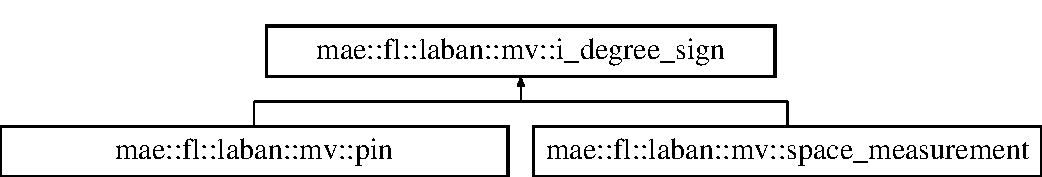
\includegraphics[height=2.000000cm]{classmae_1_1fl_1_1laban_1_1mv_1_1i__degree__sign}
\end{center}
\end{figure}
\subsection*{Public Member Functions}
\begin{DoxyCompactItemize}
\item 
virtual bool \hyperlink{classmae_1_1fl_1_1laban_1_1mv_1_1i__degree__sign_a65fee11b31d29709fd4022f90f4638bd}{equals} (std\-::shared\-\_\-ptr$<$ \hyperlink{classmae_1_1fl_1_1laban_1_1mv_1_1i__degree__sign}{i\-\_\-degree\-\_\-sign} $>$ a) const =0
\item 
virtual std\-::string \hyperlink{classmae_1_1fl_1_1laban_1_1mv_1_1i__degree__sign_abddf8459a5231b204ac2f023633aa4c4}{xml} (unsigned int indent=0, std\-::string namesp=\char`\"{}\char`\"{}, bool print\-\_\-type=false) const =0
\item 
virtual std\-::string \hyperlink{classmae_1_1fl_1_1laban_1_1mv_1_1i__degree__sign_abb3ff23c8dcaaa80b6062bf5f8162c51}{svg} (std\-::string identifier, double posx, double posy, double width, double height, bool left=false) const =0
\end{DoxyCompactItemize}


\subsection{Member Function Documentation}
\hypertarget{classmae_1_1fl_1_1laban_1_1mv_1_1i__degree__sign_a65fee11b31d29709fd4022f90f4638bd}{\index{mae\-::fl\-::laban\-::mv\-::i\-\_\-degree\-\_\-sign@{mae\-::fl\-::laban\-::mv\-::i\-\_\-degree\-\_\-sign}!equals@{equals}}
\index{equals@{equals}!mae::fl::laban::mv::i_degree_sign@{mae\-::fl\-::laban\-::mv\-::i\-\_\-degree\-\_\-sign}}
\subsubsection[{equals}]{\setlength{\rightskip}{0pt plus 5cm}virtual bool mae\-::fl\-::laban\-::mv\-::i\-\_\-degree\-\_\-sign\-::equals (
\begin{DoxyParamCaption}
\item[{std\-::shared\-\_\-ptr$<$ {\bf i\-\_\-degree\-\_\-sign} $>$}]{a}
\end{DoxyParamCaption}
) const\hspace{0.3cm}{\ttfamily [pure virtual]}}}\label{classmae_1_1fl_1_1laban_1_1mv_1_1i__degree__sign_a65fee11b31d29709fd4022f90f4638bd}
Returns true if the signs are equal.


\begin{DoxyParams}{Parameters}
{\em a} & The sign to be compared to. \\
\hline
\end{DoxyParams}
\begin{DoxyReturn}{Returns}
True if equal. 
\end{DoxyReturn}


Implemented in \hyperlink{classmae_1_1fl_1_1laban_1_1mv_1_1space__measurement_a3dd6b152d30ec2d8cf62933f09e445cd}{mae\-::fl\-::laban\-::mv\-::space\-\_\-measurement}, and \hyperlink{classmae_1_1fl_1_1laban_1_1mv_1_1pin_a49353682e373a913730f0556f8fe2963}{mae\-::fl\-::laban\-::mv\-::pin}.

\hypertarget{classmae_1_1fl_1_1laban_1_1mv_1_1i__degree__sign_abb3ff23c8dcaaa80b6062bf5f8162c51}{\index{mae\-::fl\-::laban\-::mv\-::i\-\_\-degree\-\_\-sign@{mae\-::fl\-::laban\-::mv\-::i\-\_\-degree\-\_\-sign}!svg@{svg}}
\index{svg@{svg}!mae::fl::laban::mv::i_degree_sign@{mae\-::fl\-::laban\-::mv\-::i\-\_\-degree\-\_\-sign}}
\subsubsection[{svg}]{\setlength{\rightskip}{0pt plus 5cm}virtual std\-::string mae\-::fl\-::laban\-::mv\-::i\-\_\-degree\-\_\-sign\-::svg (
\begin{DoxyParamCaption}
\item[{std\-::string}]{identifier, }
\item[{double}]{posx, }
\item[{double}]{posy, }
\item[{double}]{width, }
\item[{double}]{height, }
\item[{bool}]{left = {\ttfamily false}}
\end{DoxyParamCaption}
) const\hspace{0.3cm}{\ttfamily [pure virtual]}}}\label{classmae_1_1fl_1_1laban_1_1mv_1_1i__degree__sign_abb3ff23c8dcaaa80b6062bf5f8162c51}
Returns the S\-V\-G representation for this symbol.


\begin{DoxyParams}{Parameters}
{\em posx} & The x position. \\
\hline
{\em posy} & The y position. \\
\hline
{\em width} & The width. \\
\hline
{\em height} & The height. \\
\hline
\end{DoxyParams}
\begin{DoxyReturn}{Returns}
The S\-V\-G. 
\end{DoxyReturn}


Implemented in \hyperlink{classmae_1_1fl_1_1laban_1_1mv_1_1space__measurement_af68cab95083ca91bc99a9a45edc7ea86}{mae\-::fl\-::laban\-::mv\-::space\-\_\-measurement}, and \hyperlink{classmae_1_1fl_1_1laban_1_1mv_1_1pin_ae4af4900e50fc252ecd151da4ad2fe2a}{mae\-::fl\-::laban\-::mv\-::pin}.

\hypertarget{classmae_1_1fl_1_1laban_1_1mv_1_1i__degree__sign_abddf8459a5231b204ac2f023633aa4c4}{\index{mae\-::fl\-::laban\-::mv\-::i\-\_\-degree\-\_\-sign@{mae\-::fl\-::laban\-::mv\-::i\-\_\-degree\-\_\-sign}!xml@{xml}}
\index{xml@{xml}!mae::fl::laban::mv::i_degree_sign@{mae\-::fl\-::laban\-::mv\-::i\-\_\-degree\-\_\-sign}}
\subsubsection[{xml}]{\setlength{\rightskip}{0pt plus 5cm}virtual std\-::string mae\-::fl\-::laban\-::mv\-::i\-\_\-degree\-\_\-sign\-::xml (
\begin{DoxyParamCaption}
\item[{unsigned int}]{indent = {\ttfamily 0}, }
\item[{std\-::string}]{namesp = {\ttfamily \char`\"{}\char`\"{}}, }
\item[{bool}]{print\-\_\-type = {\ttfamily false}}
\end{DoxyParamCaption}
) const\hspace{0.3cm}{\ttfamily [pure virtual]}}}\label{classmae_1_1fl_1_1laban_1_1mv_1_1i__degree__sign_abddf8459a5231b204ac2f023633aa4c4}
Returns the X\-M\-L representation for this sign.


\begin{DoxyParams}{Parameters}
{\em indent} & The indent to be applied. \\
\hline
{\em namesp} & The namespace to be applied. \\
\hline
\end{DoxyParams}
\begin{DoxyReturn}{Returns}
The X\-M\-L string. 
\end{DoxyReturn}


Implemented in \hyperlink{classmae_1_1fl_1_1laban_1_1mv_1_1space__measurement_ab4121b6344f7dcbb4b7d11a3545de50a}{mae\-::fl\-::laban\-::mv\-::space\-\_\-measurement}, and \hyperlink{classmae_1_1fl_1_1laban_1_1mv_1_1pin_a1a253c5718b0f88e4ffb8bf06e8bff22}{mae\-::fl\-::laban\-::mv\-::pin}.



The documentation for this class was generated from the following file\-:\begin{DoxyCompactItemize}
\item 
src/mae/fl/laban/mv/i\-\_\-degree\-\_\-sign.\-hpp\end{DoxyCompactItemize}

\hypertarget{classmae_1_1fl_1_1laban_1_1mv_1_1i__dynamics__sign}{\section{mae\-:\-:fl\-:\-:laban\-:\-:mv\-:\-:i\-\_\-dynamics\-\_\-sign Class Reference}
\label{classmae_1_1fl_1_1laban_1_1mv_1_1i__dynamics__sign}\index{mae\-::fl\-::laban\-::mv\-::i\-\_\-dynamics\-\_\-sign@{mae\-::fl\-::laban\-::mv\-::i\-\_\-dynamics\-\_\-sign}}
}
Inheritance diagram for mae\-:\-:fl\-:\-:laban\-:\-:mv\-:\-:i\-\_\-dynamics\-\_\-sign\-:\begin{figure}[H]
\begin{center}
\leavevmode
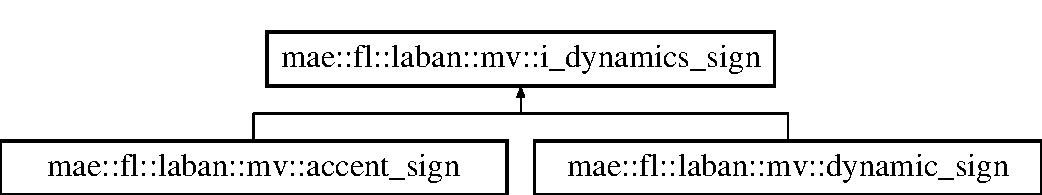
\includegraphics[height=2.000000cm]{classmae_1_1fl_1_1laban_1_1mv_1_1i__dynamics__sign}
\end{center}
\end{figure}
\subsection*{Public Member Functions}
\begin{DoxyCompactItemize}
\item 
virtual bool \hyperlink{classmae_1_1fl_1_1laban_1_1mv_1_1i__dynamics__sign_a8fe9ea5e7b50976e66172042ae01a6e3}{equals} (std\-::shared\-\_\-ptr$<$ \hyperlink{classmae_1_1fl_1_1laban_1_1mv_1_1i__dynamics__sign}{i\-\_\-dynamics\-\_\-sign} $>$ a) const =0
\item 
virtual std\-::string \hyperlink{classmae_1_1fl_1_1laban_1_1mv_1_1i__dynamics__sign_aa6332ee3990c3b59fbe8035aeae84503}{xml} (unsigned int indent=0, std\-::string namesp=\char`\"{}\char`\"{}) const =0
\end{DoxyCompactItemize}


\subsection{Member Function Documentation}
\hypertarget{classmae_1_1fl_1_1laban_1_1mv_1_1i__dynamics__sign_a8fe9ea5e7b50976e66172042ae01a6e3}{\index{mae\-::fl\-::laban\-::mv\-::i\-\_\-dynamics\-\_\-sign@{mae\-::fl\-::laban\-::mv\-::i\-\_\-dynamics\-\_\-sign}!equals@{equals}}
\index{equals@{equals}!mae::fl::laban::mv::i_dynamics_sign@{mae\-::fl\-::laban\-::mv\-::i\-\_\-dynamics\-\_\-sign}}
\subsubsection[{equals}]{\setlength{\rightskip}{0pt plus 5cm}virtual bool mae\-::fl\-::laban\-::mv\-::i\-\_\-dynamics\-\_\-sign\-::equals (
\begin{DoxyParamCaption}
\item[{std\-::shared\-\_\-ptr$<$ {\bf i\-\_\-dynamics\-\_\-sign} $>$}]{a}
\end{DoxyParamCaption}
) const\hspace{0.3cm}{\ttfamily [pure virtual]}}}\label{classmae_1_1fl_1_1laban_1_1mv_1_1i__dynamics__sign_a8fe9ea5e7b50976e66172042ae01a6e3}
Returns true if signs are equal.


\begin{DoxyParams}{Parameters}
{\em a} & The sign to be compared to. \\
\hline
\end{DoxyParams}
\begin{DoxyReturn}{Returns}
True if equal. 
\end{DoxyReturn}


Implemented in \hyperlink{classmae_1_1fl_1_1laban_1_1mv_1_1accent__sign_a891bc39b4718b06ac14243fc17667bd2}{mae\-::fl\-::laban\-::mv\-::accent\-\_\-sign}, and \hyperlink{classmae_1_1fl_1_1laban_1_1mv_1_1dynamic__sign_ac03195293621fcc14071e30179d0e5d6}{mae\-::fl\-::laban\-::mv\-::dynamic\-\_\-sign}.

\hypertarget{classmae_1_1fl_1_1laban_1_1mv_1_1i__dynamics__sign_aa6332ee3990c3b59fbe8035aeae84503}{\index{mae\-::fl\-::laban\-::mv\-::i\-\_\-dynamics\-\_\-sign@{mae\-::fl\-::laban\-::mv\-::i\-\_\-dynamics\-\_\-sign}!xml@{xml}}
\index{xml@{xml}!mae::fl::laban::mv::i_dynamics_sign@{mae\-::fl\-::laban\-::mv\-::i\-\_\-dynamics\-\_\-sign}}
\subsubsection[{xml}]{\setlength{\rightskip}{0pt plus 5cm}virtual std\-::string mae\-::fl\-::laban\-::mv\-::i\-\_\-dynamics\-\_\-sign\-::xml (
\begin{DoxyParamCaption}
\item[{unsigned int}]{indent = {\ttfamily 0}, }
\item[{std\-::string}]{namesp = {\ttfamily \char`\"{}\char`\"{}}}
\end{DoxyParamCaption}
) const\hspace{0.3cm}{\ttfamily [pure virtual]}}}\label{classmae_1_1fl_1_1laban_1_1mv_1_1i__dynamics__sign_aa6332ee3990c3b59fbe8035aeae84503}
Returns the xml string representation for the sign.


\begin{DoxyParams}{Parameters}
{\em indent} & The applied indent. \\
\hline
{\em namesp} & The namespace if any. \\
\hline
\end{DoxyParams}
\begin{DoxyReturn}{Returns}
The xml string. 
\end{DoxyReturn}


Implemented in \hyperlink{classmae_1_1fl_1_1laban_1_1mv_1_1accent__sign_a018073ffe2b04ce036e64dc5f44943de}{mae\-::fl\-::laban\-::mv\-::accent\-\_\-sign}, and \hyperlink{classmae_1_1fl_1_1laban_1_1mv_1_1dynamic__sign_a0709e2b98aaf86cb4b690f61fda62e43}{mae\-::fl\-::laban\-::mv\-::dynamic\-\_\-sign}.



The documentation for this class was generated from the following file\-:\begin{DoxyCompactItemize}
\item 
src/mae/fl/laban/mv/i\-\_\-dynamics\-\_\-sign.\-hpp\end{DoxyCompactItemize}

\hypertarget{classmae_1_1fl_1_1laban_1_1ps_1_1i__endpoint}{\section{mae\-:\-:fl\-:\-:laban\-:\-:ps\-:\-:i\-\_\-endpoint Class Reference}
\label{classmae_1_1fl_1_1laban_1_1ps_1_1i__endpoint}\index{mae\-::fl\-::laban\-::ps\-::i\-\_\-endpoint@{mae\-::fl\-::laban\-::ps\-::i\-\_\-endpoint}}
}
Inheritance diagram for mae\-:\-:fl\-:\-:laban\-:\-:ps\-:\-:i\-\_\-endpoint\-:\begin{figure}[H]
\begin{center}
\leavevmode
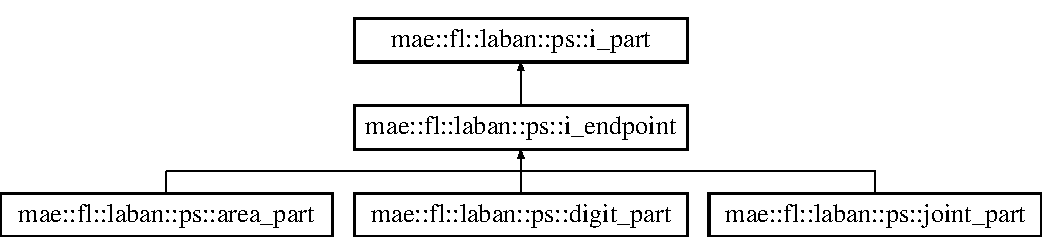
\includegraphics[height=3.000000cm]{classmae_1_1fl_1_1laban_1_1ps_1_1i__endpoint}
\end{center}
\end{figure}
\subsection*{Public Member Functions}
\begin{DoxyCompactItemize}
\item 
virtual std\-::string \hyperlink{classmae_1_1fl_1_1laban_1_1ps_1_1i__endpoint_a1af7dbd05400cbdd7f9f45ef75dd38d6}{xml} (unsigned int indent=0, std\-::string namesp=\char`\"{}\char`\"{}) const =0
\item 
virtual std\-::shared\-\_\-ptr\\*
$<$ \hyperlink{classmae_1_1fl_1_1laban_1_1ps_1_1i__endpoint}{i\-\_\-endpoint} $>$ \hyperlink{classmae_1_1fl_1_1laban_1_1ps_1_1i__endpoint_a0938824cc5892b072636c3b52352b3f2}{get\-\_\-fixed\-\_\-end} () const =0
\item 
virtual bool \hyperlink{classmae_1_1fl_1_1laban_1_1ps_1_1i__endpoint_abc675b07d3ce69fbec362b2e792a1e06}{equals} (std\-::shared\-\_\-ptr$<$ \hyperlink{classmae_1_1fl_1_1laban_1_1ps_1_1i__part}{i\-\_\-part} $>$ a) const =0
\item 
virtual bool \hyperlink{classmae_1_1fl_1_1laban_1_1ps_1_1i__endpoint_aeffb14c43728d2ef094122f3d0278455}{equals} (std\-::shared\-\_\-ptr$<$ \hyperlink{classmae_1_1fl_1_1laban_1_1ps_1_1i__endpoint}{i\-\_\-endpoint} $>$ a) const =0
\end{DoxyCompactItemize}


\subsection{Member Function Documentation}
\hypertarget{classmae_1_1fl_1_1laban_1_1ps_1_1i__endpoint_abc675b07d3ce69fbec362b2e792a1e06}{\index{mae\-::fl\-::laban\-::ps\-::i\-\_\-endpoint@{mae\-::fl\-::laban\-::ps\-::i\-\_\-endpoint}!equals@{equals}}
\index{equals@{equals}!mae::fl::laban::ps::i_endpoint@{mae\-::fl\-::laban\-::ps\-::i\-\_\-endpoint}}
\subsubsection[{equals}]{\setlength{\rightskip}{0pt plus 5cm}virtual bool mae\-::fl\-::laban\-::ps\-::i\-\_\-endpoint\-::equals (
\begin{DoxyParamCaption}
\item[{std\-::shared\-\_\-ptr$<$ {\bf i\-\_\-part} $>$}]{a}
\end{DoxyParamCaption}
) const\hspace{0.3cm}{\ttfamily [pure virtual]}}}\label{classmae_1_1fl_1_1laban_1_1ps_1_1i__endpoint_abc675b07d3ce69fbec362b2e792a1e06}
Returns true if elements are equal.


\begin{DoxyParams}{Parameters}
{\em a} & The element to be compared to. \\
\hline
\end{DoxyParams}
\begin{DoxyReturn}{Returns}
True if equal. 
\end{DoxyReturn}


Implements \hyperlink{classmae_1_1fl_1_1laban_1_1ps_1_1i__part_ad43f6b88cb409ac26342db51606ea1e1}{mae\-::fl\-::laban\-::ps\-::i\-\_\-part}.



Implemented in \hyperlink{classmae_1_1fl_1_1laban_1_1ps_1_1digit__part_a6bcdd921e55c60908e827534d4957c4d}{mae\-::fl\-::laban\-::ps\-::digit\-\_\-part}, \hyperlink{classmae_1_1fl_1_1laban_1_1ps_1_1area__part_aa223417cb9c21426014d0099f9fad72b}{mae\-::fl\-::laban\-::ps\-::area\-\_\-part}, and \hyperlink{classmae_1_1fl_1_1laban_1_1ps_1_1joint__part_a1de75536e4a12e1435e0ec3c4f2edbad}{mae\-::fl\-::laban\-::ps\-::joint\-\_\-part}.

\hypertarget{classmae_1_1fl_1_1laban_1_1ps_1_1i__endpoint_aeffb14c43728d2ef094122f3d0278455}{\index{mae\-::fl\-::laban\-::ps\-::i\-\_\-endpoint@{mae\-::fl\-::laban\-::ps\-::i\-\_\-endpoint}!equals@{equals}}
\index{equals@{equals}!mae::fl::laban::ps::i_endpoint@{mae\-::fl\-::laban\-::ps\-::i\-\_\-endpoint}}
\subsubsection[{equals}]{\setlength{\rightskip}{0pt plus 5cm}virtual bool mae\-::fl\-::laban\-::ps\-::i\-\_\-endpoint\-::equals (
\begin{DoxyParamCaption}
\item[{std\-::shared\-\_\-ptr$<$ {\bf i\-\_\-endpoint} $>$}]{a}
\end{DoxyParamCaption}
) const\hspace{0.3cm}{\ttfamily [pure virtual]}}}\label{classmae_1_1fl_1_1laban_1_1ps_1_1i__endpoint_aeffb14c43728d2ef094122f3d0278455}
Returns true if elements are equal.


\begin{DoxyParams}{Parameters}
{\em a} & The element to be compared to. \\
\hline
\end{DoxyParams}
\begin{DoxyReturn}{Returns}
True if equal. 
\end{DoxyReturn}


Implemented in \hyperlink{classmae_1_1fl_1_1laban_1_1ps_1_1digit__part_a0966a987076279fe198566b953bbc7a3}{mae\-::fl\-::laban\-::ps\-::digit\-\_\-part}, \hyperlink{classmae_1_1fl_1_1laban_1_1ps_1_1area__part_af1715756d2b703af8ea2d7549ff7a6fc}{mae\-::fl\-::laban\-::ps\-::area\-\_\-part}, and \hyperlink{classmae_1_1fl_1_1laban_1_1ps_1_1joint__part_ad159de6d5a1adb07b76a4a151541569e}{mae\-::fl\-::laban\-::ps\-::joint\-\_\-part}.

\hypertarget{classmae_1_1fl_1_1laban_1_1ps_1_1i__endpoint_a0938824cc5892b072636c3b52352b3f2}{\index{mae\-::fl\-::laban\-::ps\-::i\-\_\-endpoint@{mae\-::fl\-::laban\-::ps\-::i\-\_\-endpoint}!get\-\_\-fixed\-\_\-end@{get\-\_\-fixed\-\_\-end}}
\index{get\-\_\-fixed\-\_\-end@{get\-\_\-fixed\-\_\-end}!mae::fl::laban::ps::i_endpoint@{mae\-::fl\-::laban\-::ps\-::i\-\_\-endpoint}}
\subsubsection[{get\-\_\-fixed\-\_\-end}]{\setlength{\rightskip}{0pt plus 5cm}virtual std\-::shared\-\_\-ptr$<${\bf i\-\_\-endpoint}$>$ mae\-::fl\-::laban\-::ps\-::i\-\_\-endpoint\-::get\-\_\-fixed\-\_\-end (
\begin{DoxyParamCaption}
{}
\end{DoxyParamCaption}
) const\hspace{0.3cm}{\ttfamily [pure virtual]}}}\label{classmae_1_1fl_1_1laban_1_1ps_1_1i__endpoint_a0938824cc5892b072636c3b52352b3f2}
Returns the predecessor of the current endpoint (which is the default fixed endpoint). If the endpoint is the beginning of the extremity null is returned.

\begin{DoxyReturn}{Returns}
The successor element. 
\end{DoxyReturn}


Implemented in \hyperlink{classmae_1_1fl_1_1laban_1_1ps_1_1digit__part_ad8f600cbaccf7194ea70c93432a1e9b5}{mae\-::fl\-::laban\-::ps\-::digit\-\_\-part}, \hyperlink{classmae_1_1fl_1_1laban_1_1ps_1_1area__part_ad3697cd7f8840ff9341da918cd7f84f5}{mae\-::fl\-::laban\-::ps\-::area\-\_\-part}, and \hyperlink{classmae_1_1fl_1_1laban_1_1ps_1_1joint__part_a08d427668f18131036b88c2156ccdd3f}{mae\-::fl\-::laban\-::ps\-::joint\-\_\-part}.

\hypertarget{classmae_1_1fl_1_1laban_1_1ps_1_1i__endpoint_a1af7dbd05400cbdd7f9f45ef75dd38d6}{\index{mae\-::fl\-::laban\-::ps\-::i\-\_\-endpoint@{mae\-::fl\-::laban\-::ps\-::i\-\_\-endpoint}!xml@{xml}}
\index{xml@{xml}!mae::fl::laban::ps::i_endpoint@{mae\-::fl\-::laban\-::ps\-::i\-\_\-endpoint}}
\subsubsection[{xml}]{\setlength{\rightskip}{0pt plus 5cm}virtual std\-::string mae\-::fl\-::laban\-::ps\-::i\-\_\-endpoint\-::xml (
\begin{DoxyParamCaption}
\item[{unsigned int}]{indent = {\ttfamily 0}, }
\item[{std\-::string}]{namesp = {\ttfamily \char`\"{}\char`\"{}}}
\end{DoxyParamCaption}
) const\hspace{0.3cm}{\ttfamily [pure virtual]}}}\label{classmae_1_1fl_1_1laban_1_1ps_1_1i__endpoint_a1af7dbd05400cbdd7f9f45ef75dd38d6}
Returns the X\-M\-L representation for this element.


\begin{DoxyParams}{Parameters}
{\em indent} & The applied indent. \\
\hline
{\em namesp} & The prefixed X\-M\-L namespace.\\
\hline
\end{DoxyParams}
\begin{DoxyReturn}{Returns}
The X\-M\-L string. 
\end{DoxyReturn}


Implements \hyperlink{classmae_1_1fl_1_1laban_1_1ps_1_1i__part_a704c07899099cdf53beb9187f23b7874}{mae\-::fl\-::laban\-::ps\-::i\-\_\-part}.



Implemented in \hyperlink{classmae_1_1fl_1_1laban_1_1ps_1_1digit__part_a51e9b056b0d57310e1423efbf8ebec48}{mae\-::fl\-::laban\-::ps\-::digit\-\_\-part}, \hyperlink{classmae_1_1fl_1_1laban_1_1ps_1_1area__part_a3ffd61d8cba76a5312a737a40dccb4ec}{mae\-::fl\-::laban\-::ps\-::area\-\_\-part}, and \hyperlink{classmae_1_1fl_1_1laban_1_1ps_1_1joint__part_a3054936a94c43d4cb3cb21745234e2cf}{mae\-::fl\-::laban\-::ps\-::joint\-\_\-part}.



The documentation for this class was generated from the following file\-:\begin{DoxyCompactItemize}
\item 
src/mae/fl/laban/ps/i\-\_\-endpoint.\-hpp\end{DoxyCompactItemize}

\hypertarget{classmae_1_1i__kp__detector}{\section{mae\-:\-:i\-\_\-kp\-\_\-detector Class Reference}
\label{classmae_1_1i__kp__detector}\index{mae\-::i\-\_\-kp\-\_\-detector@{mae\-::i\-\_\-kp\-\_\-detector}}
}
Inheritance diagram for mae\-:\-:i\-\_\-kp\-\_\-detector\-:\begin{figure}[H]
\begin{center}
\leavevmode
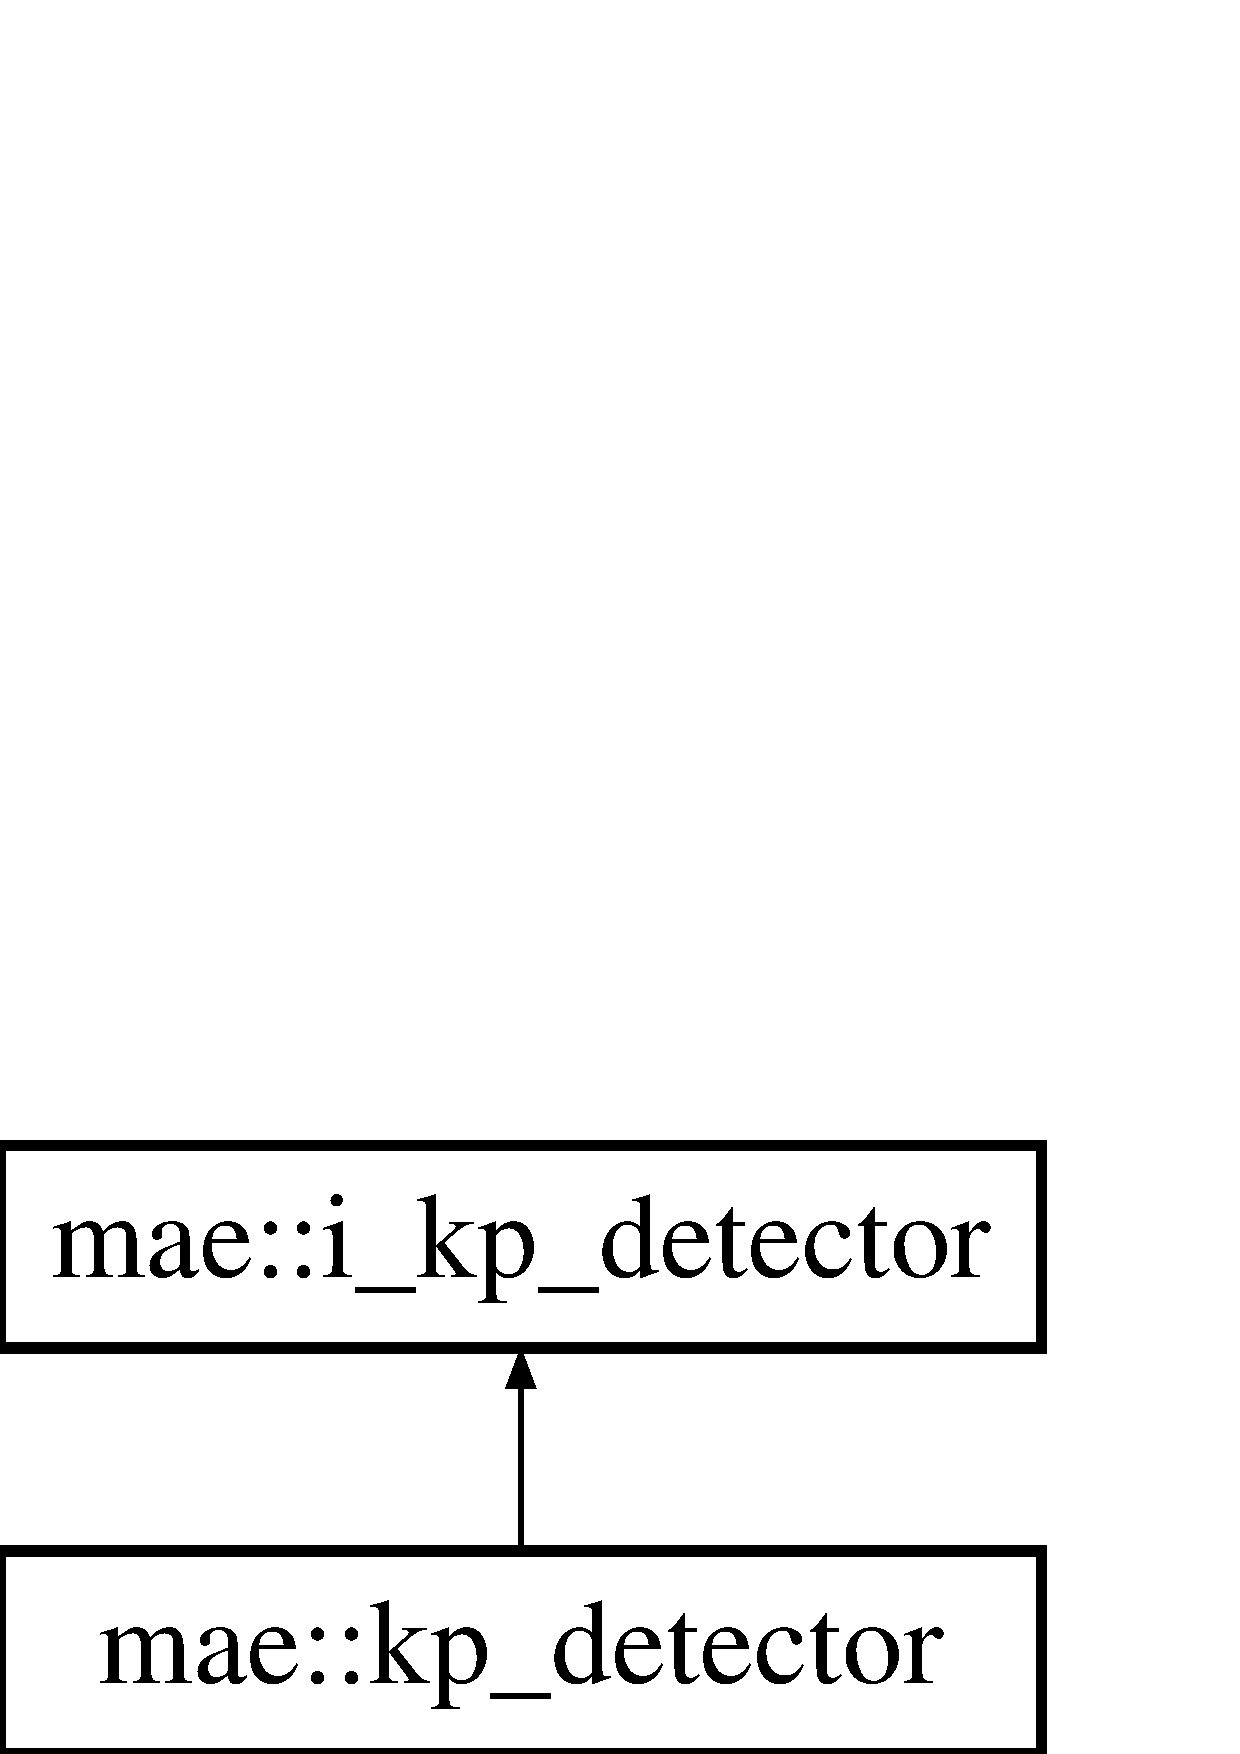
\includegraphics[height=2.000000cm]{classmae_1_1i__kp__detector}
\end{center}
\end{figure}
\subsection*{Public Member Functions}
\begin{DoxyCompactItemize}
\item 
virtual std\-::shared\-\_\-ptr\\*
$<$ \hyperlink{classmae_1_1general__enriched__pose}{general\-\_\-enriched\-\_\-pose} $>$ \hyperlink{classmae_1_1i__kp__detector_a42a950416d5bc959544c0138a8526847}{estimate\-\_\-frame} (double framerate, std\-::shared\-\_\-ptr$<$ \hyperlink{classmae_1_1general__pose}{general\-\_\-pose} $>$ current\-Pose, std\-::list$<$ std\-::shared\-\_\-ptr$<$ \hyperlink{classmae_1_1general__enriched__pose}{general\-\_\-enriched\-\_\-pose} $>$ $>$ previous\-Sequence, std\-::vector$<$ \hyperlink{classmae_1_1bone}{bone} $>$ body\-Parts)=0
\end{DoxyCompactItemize}


\subsection{Member Function Documentation}
\hypertarget{classmae_1_1i__kp__detector_a42a950416d5bc959544c0138a8526847}{\index{mae\-::i\-\_\-kp\-\_\-detector@{mae\-::i\-\_\-kp\-\_\-detector}!estimate\-\_\-frame@{estimate\-\_\-frame}}
\index{estimate\-\_\-frame@{estimate\-\_\-frame}!mae::i_kp_detector@{mae\-::i\-\_\-kp\-\_\-detector}}
\subsubsection[{estimate\-\_\-frame}]{\setlength{\rightskip}{0pt plus 5cm}virtual std\-::shared\-\_\-ptr$<${\bf general\-\_\-enriched\-\_\-pose}$>$ mae\-::i\-\_\-kp\-\_\-detector\-::estimate\-\_\-frame (
\begin{DoxyParamCaption}
\item[{double}]{framerate, }
\item[{std\-::shared\-\_\-ptr$<$ {\bf general\-\_\-pose} $>$}]{current\-Pose, }
\item[{std\-::list$<$ std\-::shared\-\_\-ptr$<$ {\bf general\-\_\-enriched\-\_\-pose} $>$ $>$}]{previous\-Sequence, }
\item[{std\-::vector$<$ {\bf bone} $>$}]{body\-Parts}
\end{DoxyParamCaption}
)\hspace{0.3cm}{\ttfamily [pure virtual]}}}\label{classmae_1_1i__kp__detector_a42a950416d5bc959544c0138a8526847}
Estimates the current frame and returns an enriched pose. Edits the given enriched poses, (e.\-g. sets key pose to false) but does not append the new enriched pose to the vector. Instead the new enriched pose is returned.


\begin{DoxyParams}{Parameters}
{\em framerate} & The framerate. \\
\hline
{\em current\-Pose} & The currently processed pose. \\
\hline
{\em previous\-Sequence} & The previous sequence which will be edited too. \\
\hline
{\em body\-Parts} & All body parts that shall be processed. \\
\hline
\end{DoxyParams}
\begin{DoxyReturn}{Returns}
The enriched pose. 
\end{DoxyReturn}


Implemented in \hyperlink{classmae_1_1kp__detector_a782a911f14f742f1ddbe4df9cdeb8f7c}{mae\-::kp\-\_\-detector}.



The documentation for this class was generated from the following file\-:\begin{DoxyCompactItemize}
\item 
src/mae/i\-\_\-kp\-\_\-detector.\-hpp\end{DoxyCompactItemize}

\hypertarget{classmae_1_1fl_1_1laban_1_1ps_1_1i__limb}{\section{mae\-:\-:fl\-:\-:laban\-:\-:ps\-:\-:i\-\_\-limb Class Reference}
\label{classmae_1_1fl_1_1laban_1_1ps_1_1i__limb}\index{mae\-::fl\-::laban\-::ps\-::i\-\_\-limb@{mae\-::fl\-::laban\-::ps\-::i\-\_\-limb}}
}
Inheritance diagram for mae\-:\-:fl\-:\-:laban\-:\-:ps\-:\-:i\-\_\-limb\-:\begin{figure}[H]
\begin{center}
\leavevmode
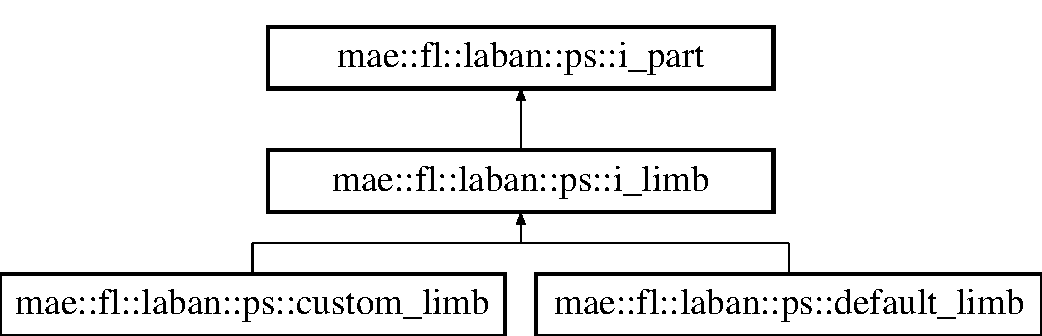
\includegraphics[height=3.000000cm]{classmae_1_1fl_1_1laban_1_1ps_1_1i__limb}
\end{center}
\end{figure}
\subsection*{Public Member Functions}
\begin{DoxyCompactItemize}
\item 
virtual std\-::string \hyperlink{classmae_1_1fl_1_1laban_1_1ps_1_1i__limb_a7a5c3ca32936748a1e60fdab1d29b1c9}{xml} (unsigned int indent=0, std\-::string namesp=\char`\"{}\char`\"{}) const =0
\item 
virtual bool \hyperlink{classmae_1_1fl_1_1laban_1_1ps_1_1i__limb_aa46cb4b952cc2a8692f3f32895a28041}{equals} (std\-::shared\-\_\-ptr$<$ \hyperlink{classmae_1_1fl_1_1laban_1_1ps_1_1i__part}{i\-\_\-part} $>$ a) const =0
\item 
virtual bool \hyperlink{classmae_1_1fl_1_1laban_1_1ps_1_1i__limb_a7e7ba568e9711b8901234f2cb73b67b8}{equals} (std\-::shared\-\_\-ptr$<$ \hyperlink{classmae_1_1fl_1_1laban_1_1ps_1_1i__limb}{i\-\_\-limb} $>$ a) const =0
\end{DoxyCompactItemize}


\subsection{Member Function Documentation}
\hypertarget{classmae_1_1fl_1_1laban_1_1ps_1_1i__limb_aa46cb4b952cc2a8692f3f32895a28041}{\index{mae\-::fl\-::laban\-::ps\-::i\-\_\-limb@{mae\-::fl\-::laban\-::ps\-::i\-\_\-limb}!equals@{equals}}
\index{equals@{equals}!mae::fl::laban::ps::i_limb@{mae\-::fl\-::laban\-::ps\-::i\-\_\-limb}}
\subsubsection[{equals}]{\setlength{\rightskip}{0pt plus 5cm}virtual bool mae\-::fl\-::laban\-::ps\-::i\-\_\-limb\-::equals (
\begin{DoxyParamCaption}
\item[{std\-::shared\-\_\-ptr$<$ {\bf i\-\_\-part} $>$}]{a}
\end{DoxyParamCaption}
) const\hspace{0.3cm}{\ttfamily [pure virtual]}}}\label{classmae_1_1fl_1_1laban_1_1ps_1_1i__limb_aa46cb4b952cc2a8692f3f32895a28041}
Returns true if elements are equal.


\begin{DoxyParams}{Parameters}
{\em a} & The element to be compared to. \\
\hline
\end{DoxyParams}
\begin{DoxyReturn}{Returns}
True if equal. 
\end{DoxyReturn}


Implements \hyperlink{classmae_1_1fl_1_1laban_1_1ps_1_1i__part_ad43f6b88cb409ac26342db51606ea1e1}{mae\-::fl\-::laban\-::ps\-::i\-\_\-part}.



Implemented in \hyperlink{classmae_1_1fl_1_1laban_1_1ps_1_1custom__limb_aea87a1c04a4a8fde3ef80862690b0318}{mae\-::fl\-::laban\-::ps\-::custom\-\_\-limb}, and \hyperlink{classmae_1_1fl_1_1laban_1_1ps_1_1default__limb_a9bdae13195e31e15c5511dcf04786aae}{mae\-::fl\-::laban\-::ps\-::default\-\_\-limb}.

\hypertarget{classmae_1_1fl_1_1laban_1_1ps_1_1i__limb_a7e7ba568e9711b8901234f2cb73b67b8}{\index{mae\-::fl\-::laban\-::ps\-::i\-\_\-limb@{mae\-::fl\-::laban\-::ps\-::i\-\_\-limb}!equals@{equals}}
\index{equals@{equals}!mae::fl::laban::ps::i_limb@{mae\-::fl\-::laban\-::ps\-::i\-\_\-limb}}
\subsubsection[{equals}]{\setlength{\rightskip}{0pt plus 5cm}virtual bool mae\-::fl\-::laban\-::ps\-::i\-\_\-limb\-::equals (
\begin{DoxyParamCaption}
\item[{std\-::shared\-\_\-ptr$<$ {\bf i\-\_\-limb} $>$}]{a}
\end{DoxyParamCaption}
) const\hspace{0.3cm}{\ttfamily [pure virtual]}}}\label{classmae_1_1fl_1_1laban_1_1ps_1_1i__limb_a7e7ba568e9711b8901234f2cb73b67b8}
Returns true if elements are equal.


\begin{DoxyParams}{Parameters}
{\em a} & The element to be compared to. \\
\hline
\end{DoxyParams}
\begin{DoxyReturn}{Returns}
True if equal. 
\end{DoxyReturn}


Implemented in \hyperlink{classmae_1_1fl_1_1laban_1_1ps_1_1custom__limb_ab152826ff0de843c52695807715a6c71}{mae\-::fl\-::laban\-::ps\-::custom\-\_\-limb}, and \hyperlink{classmae_1_1fl_1_1laban_1_1ps_1_1default__limb_ae7d58fdb145ee8c34b6f221ac0752b01}{mae\-::fl\-::laban\-::ps\-::default\-\_\-limb}.

\hypertarget{classmae_1_1fl_1_1laban_1_1ps_1_1i__limb_a7a5c3ca32936748a1e60fdab1d29b1c9}{\index{mae\-::fl\-::laban\-::ps\-::i\-\_\-limb@{mae\-::fl\-::laban\-::ps\-::i\-\_\-limb}!xml@{xml}}
\index{xml@{xml}!mae::fl::laban::ps::i_limb@{mae\-::fl\-::laban\-::ps\-::i\-\_\-limb}}
\subsubsection[{xml}]{\setlength{\rightskip}{0pt plus 5cm}virtual std\-::string mae\-::fl\-::laban\-::ps\-::i\-\_\-limb\-::xml (
\begin{DoxyParamCaption}
\item[{unsigned int}]{indent = {\ttfamily 0}, }
\item[{std\-::string}]{namesp = {\ttfamily \char`\"{}\char`\"{}}}
\end{DoxyParamCaption}
) const\hspace{0.3cm}{\ttfamily [pure virtual]}}}\label{classmae_1_1fl_1_1laban_1_1ps_1_1i__limb_a7a5c3ca32936748a1e60fdab1d29b1c9}
Returns the X\-M\-L representation for this element.


\begin{DoxyParams}{Parameters}
{\em indent} & The applied indent. \\
\hline
{\em namesp} & The prefixed X\-M\-L namespace.\\
\hline
\end{DoxyParams}
\begin{DoxyReturn}{Returns}
The X\-M\-L string. 
\end{DoxyReturn}


Implements \hyperlink{classmae_1_1fl_1_1laban_1_1ps_1_1i__part_a704c07899099cdf53beb9187f23b7874}{mae\-::fl\-::laban\-::ps\-::i\-\_\-part}.



Implemented in \hyperlink{classmae_1_1fl_1_1laban_1_1ps_1_1custom__limb_a2622dd693ce2f662a4802025b42f1e64}{mae\-::fl\-::laban\-::ps\-::custom\-\_\-limb}, and \hyperlink{classmae_1_1fl_1_1laban_1_1ps_1_1default__limb_a1d266ba068ce557431a90476b0ce3a82}{mae\-::fl\-::laban\-::ps\-::default\-\_\-limb}.



The documentation for this class was generated from the following file\-:\begin{DoxyCompactItemize}
\item 
src/mae/fl/laban/ps/i\-\_\-limb.\-hpp\end{DoxyCompactItemize}

\hypertarget{classmae_1_1fl_1_1laban_1_1i__movement}{\section{mae\-:\-:fl\-:\-:laban\-:\-:i\-\_\-movement Class Reference}
\label{classmae_1_1fl_1_1laban_1_1i__movement}\index{mae\-::fl\-::laban\-::i\-\_\-movement@{mae\-::fl\-::laban\-::i\-\_\-movement}}
}
Inheritance diagram for mae\-:\-:fl\-:\-:laban\-:\-:i\-\_\-movement\-:\begin{figure}[H]
\begin{center}
\leavevmode
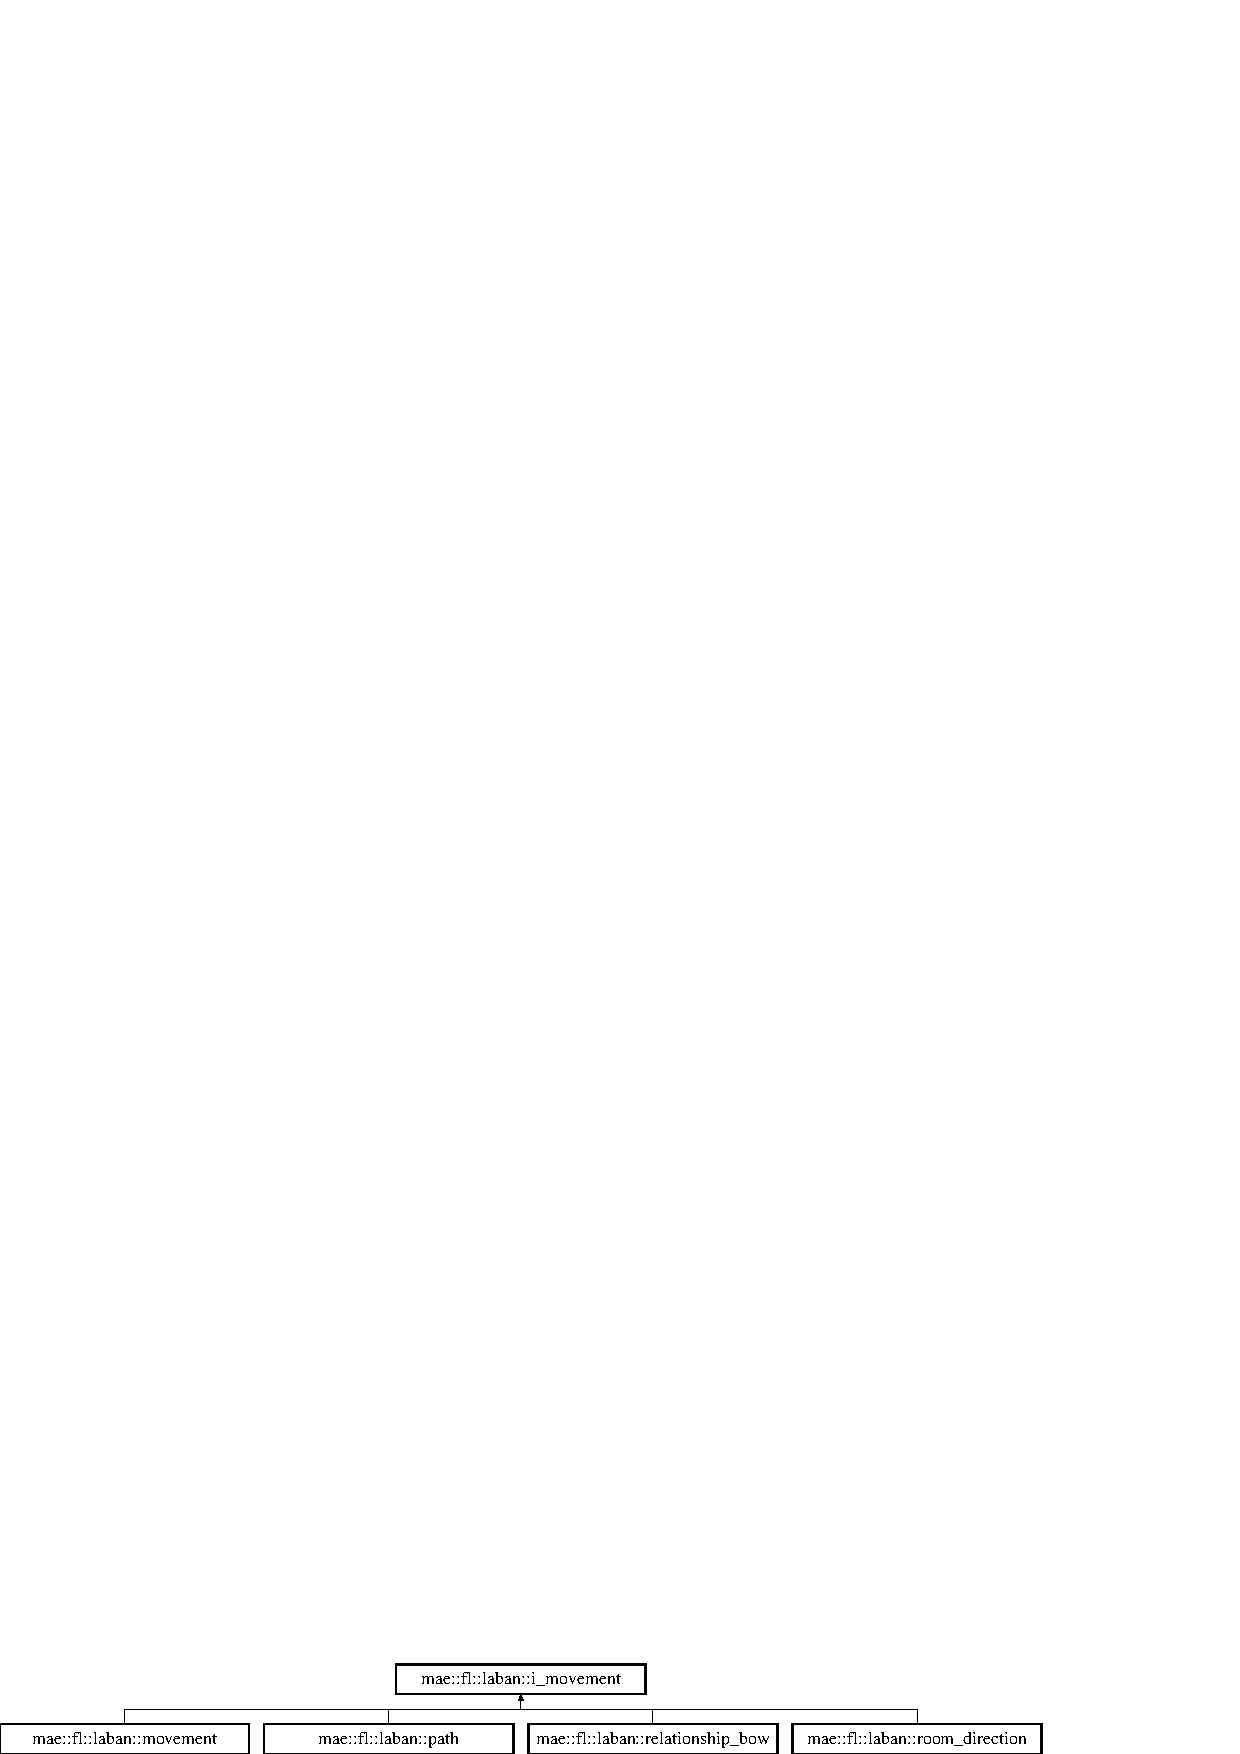
\includegraphics[height=1.443299cm]{classmae_1_1fl_1_1laban_1_1i__movement}
\end{center}
\end{figure}
\subsection*{Public Member Functions}
\begin{DoxyCompactItemize}
\item 
virtual int \hyperlink{classmae_1_1fl_1_1laban_1_1i__movement_a448424f76457ed1dfa28e5d2c774c311}{get\-\_\-column} () const =0
\item 
virtual unsigned int \hyperlink{classmae_1_1fl_1_1laban_1_1i__movement_aa1b18a889adea3d1aa8a5a8af5de2de6}{get\-\_\-measure} () const =0
\item 
virtual double \hyperlink{classmae_1_1fl_1_1laban_1_1i__movement_a2b8ee7b4d5cb5be09be93ff049fbdc68}{get\-\_\-beat} () const =0
\item 
virtual double \hyperlink{classmae_1_1fl_1_1laban_1_1i__movement_ac83194ad9df8fed6c27199e83d35460d}{get\-\_\-duration} () const =0
\item 
virtual bool \hyperlink{classmae_1_1fl_1_1laban_1_1i__movement_a29783771372283ff2cc7deded01b83b1}{equals} (std\-::shared\-\_\-ptr$<$ \hyperlink{classmae_1_1fl_1_1laban_1_1i__movement}{i\-\_\-movement} $>$ a) const =0
\item 
virtual bool \hyperlink{classmae_1_1fl_1_1laban_1_1i__movement_a7b682911356dd13497172280b268ec40}{symbol\-\_\-equals} (std\-::shared\-\_\-ptr$<$ \hyperlink{classmae_1_1fl_1_1laban_1_1i__movement}{i\-\_\-movement} $>$ a) const =0
\item 
virtual std\-::string \hyperlink{classmae_1_1fl_1_1laban_1_1i__movement_acd832b2a6976bfe32eae4bece01ee8f3}{xml} (unsigned int indent=0, std\-::string namesp=\char`\"{}\char`\"{}) const =0
\item 
virtual std\-::string \hyperlink{classmae_1_1fl_1_1laban_1_1i__movement_ab2b0225ae8237b8ae410c797a0319498}{svg} (unsigned int im\-\_\-width, unsigned int im\-\_\-height, unsigned int max\-\_\-column, unsigned int measures, unsigned int beats\-\_\-per\-\_\-measure) const =0
\item 
virtual std\-::shared\-\_\-ptr\\*
$<$ \hyperlink{classmae_1_1fl_1_1laban_1_1i__movement}{i\-\_\-movement} $>$ \hyperlink{classmae_1_1fl_1_1laban_1_1i__movement_a28c8b00c68e291399281bda22e4f01f6}{recreate} (std\-::map$<$ int, int $>$ column\-\_\-mapping, unsigned int measure, double beat, double duration) const =0
\item 
virtual std\-::string \hyperlink{classmae_1_1fl_1_1laban_1_1i__movement_a18322189d1851d3fd0f85c00b1051b57}{str} () const =0
\end{DoxyCompactItemize}
\subsection*{Friends}
\begin{DoxyCompactItemize}
\item 
\hypertarget{classmae_1_1fl_1_1laban_1_1i__movement_af67c69d4e1d111e0ffda350a661c57e4}{std\-::ostream \& {\bfseries operator$<$$<$} (std\-::ostream \&os, const \hyperlink{classmae_1_1fl_1_1laban_1_1i__movement}{i\-\_\-movement} \&obj)}\label{classmae_1_1fl_1_1laban_1_1i__movement_af67c69d4e1d111e0ffda350a661c57e4}

\item 
\hypertarget{classmae_1_1fl_1_1laban_1_1i__movement_afd9ce7f9bc5e2155bb74ee262404cc3d}{std\-::ostream \& {\bfseries operator$<$$<$} (std\-::ostream \&os, const std\-::shared\-\_\-ptr$<$ \hyperlink{classmae_1_1fl_1_1laban_1_1i__movement}{i\-\_\-movement} $>$ \&obj)}\label{classmae_1_1fl_1_1laban_1_1i__movement_afd9ce7f9bc5e2155bb74ee262404cc3d}

\end{DoxyCompactItemize}


\subsection{Member Function Documentation}
\hypertarget{classmae_1_1fl_1_1laban_1_1i__movement_a29783771372283ff2cc7deded01b83b1}{\index{mae\-::fl\-::laban\-::i\-\_\-movement@{mae\-::fl\-::laban\-::i\-\_\-movement}!equals@{equals}}
\index{equals@{equals}!mae::fl::laban::i_movement@{mae\-::fl\-::laban\-::i\-\_\-movement}}
\subsubsection[{equals}]{\setlength{\rightskip}{0pt plus 5cm}virtual bool mae\-::fl\-::laban\-::i\-\_\-movement\-::equals (
\begin{DoxyParamCaption}
\item[{std\-::shared\-\_\-ptr$<$ {\bf i\-\_\-movement} $>$}]{a}
\end{DoxyParamCaption}
) const\hspace{0.3cm}{\ttfamily [pure virtual]}}}\label{classmae_1_1fl_1_1laban_1_1i__movement_a29783771372283ff2cc7deded01b83b1}
Returns true if the \hyperlink{classmae_1_1fl_1_1laban_1_1i__movement}{i\-\_\-movement} elements are equal.


\begin{DoxyParams}{Parameters}
{\em a} & The movement to be compared to. \\
\hline
\end{DoxyParams}
\begin{DoxyReturn}{Returns}
True if equal. 
\end{DoxyReturn}


Implemented in \hyperlink{classmae_1_1fl_1_1laban_1_1relationship__bow_a528d367eeff4bfcff462b201187b3bfc}{mae\-::fl\-::laban\-::relationship\-\_\-bow}, \hyperlink{classmae_1_1fl_1_1laban_1_1movement_a93b7f317d4ba358a641b43a21c09f228}{mae\-::fl\-::laban\-::movement}, \hyperlink{classmae_1_1fl_1_1laban_1_1room__direction_a87704a471c16270f08a1b9f9ded7618d}{mae\-::fl\-::laban\-::room\-\_\-direction}, and \hyperlink{classmae_1_1fl_1_1laban_1_1path_ade22858a457d91a3faa2a3eee14d66be}{mae\-::fl\-::laban\-::path}.

\hypertarget{classmae_1_1fl_1_1laban_1_1i__movement_a2b8ee7b4d5cb5be09be93ff049fbdc68}{\index{mae\-::fl\-::laban\-::i\-\_\-movement@{mae\-::fl\-::laban\-::i\-\_\-movement}!get\-\_\-beat@{get\-\_\-beat}}
\index{get\-\_\-beat@{get\-\_\-beat}!mae::fl::laban::i_movement@{mae\-::fl\-::laban\-::i\-\_\-movement}}
\subsubsection[{get\-\_\-beat}]{\setlength{\rightskip}{0pt plus 5cm}virtual double mae\-::fl\-::laban\-::i\-\_\-movement\-::get\-\_\-beat (
\begin{DoxyParamCaption}
{}
\end{DoxyParamCaption}
) const\hspace{0.3cm}{\ttfamily [pure virtual]}}}\label{classmae_1_1fl_1_1laban_1_1i__movement_a2b8ee7b4d5cb5be09be93ff049fbdc68}
Returns the beat in which this symbol begins.

\begin{DoxyReturn}{Returns}

\end{DoxyReturn}


Implemented in \hyperlink{classmae_1_1fl_1_1laban_1_1relationship__bow_a0fe4d1a9fd99e3c2e5daab7c5e3ffb6a}{mae\-::fl\-::laban\-::relationship\-\_\-bow}, \hyperlink{classmae_1_1fl_1_1laban_1_1movement_a8dd1f022fc3402ece07a15863416d80a}{mae\-::fl\-::laban\-::movement}, \hyperlink{classmae_1_1fl_1_1laban_1_1path_ad7f035766edfa9f6f9f2037c26fc3309}{mae\-::fl\-::laban\-::path}, and \hyperlink{classmae_1_1fl_1_1laban_1_1room__direction_ad1b05ee39b84fc937170b2ef90af6f71}{mae\-::fl\-::laban\-::room\-\_\-direction}.

\hypertarget{classmae_1_1fl_1_1laban_1_1i__movement_a448424f76457ed1dfa28e5d2c774c311}{\index{mae\-::fl\-::laban\-::i\-\_\-movement@{mae\-::fl\-::laban\-::i\-\_\-movement}!get\-\_\-column@{get\-\_\-column}}
\index{get\-\_\-column@{get\-\_\-column}!mae::fl::laban::i_movement@{mae\-::fl\-::laban\-::i\-\_\-movement}}
\subsubsection[{get\-\_\-column}]{\setlength{\rightskip}{0pt plus 5cm}virtual int mae\-::fl\-::laban\-::i\-\_\-movement\-::get\-\_\-column (
\begin{DoxyParamCaption}
{}
\end{DoxyParamCaption}
) const\hspace{0.3cm}{\ttfamily [pure virtual]}}}\label{classmae_1_1fl_1_1laban_1_1i__movement_a448424f76457ed1dfa28e5d2c774c311}
Returns the column this movement is attached to. Room direction and path sign have their own specific column only for those signs and therefore return 0.

\begin{DoxyReturn}{Returns}
The column id. 
\end{DoxyReturn}


Implemented in \hyperlink{classmae_1_1fl_1_1laban_1_1relationship__bow_ada0c5d5f50bb062ba2c4a5afae33d76a}{mae\-::fl\-::laban\-::relationship\-\_\-bow}, \hyperlink{classmae_1_1fl_1_1laban_1_1path_a6a842cc38fccadb4d9deca546fce3e63}{mae\-::fl\-::laban\-::path}, \hyperlink{classmae_1_1fl_1_1laban_1_1movement_a7c6e91fd57b5cbec8d5d32901c9897d2}{mae\-::fl\-::laban\-::movement}, and \hyperlink{classmae_1_1fl_1_1laban_1_1room__direction_afa452f53f560485183e322571c9d1931}{mae\-::fl\-::laban\-::room\-\_\-direction}.

\hypertarget{classmae_1_1fl_1_1laban_1_1i__movement_ac83194ad9df8fed6c27199e83d35460d}{\index{mae\-::fl\-::laban\-::i\-\_\-movement@{mae\-::fl\-::laban\-::i\-\_\-movement}!get\-\_\-duration@{get\-\_\-duration}}
\index{get\-\_\-duration@{get\-\_\-duration}!mae::fl::laban::i_movement@{mae\-::fl\-::laban\-::i\-\_\-movement}}
\subsubsection[{get\-\_\-duration}]{\setlength{\rightskip}{0pt plus 5cm}virtual double mae\-::fl\-::laban\-::i\-\_\-movement\-::get\-\_\-duration (
\begin{DoxyParamCaption}
{}
\end{DoxyParamCaption}
) const\hspace{0.3cm}{\ttfamily [pure virtual]}}}\label{classmae_1_1fl_1_1laban_1_1i__movement_ac83194ad9df8fed6c27199e83d35460d}
Returns the duration of the symbol. Room direction symbols do not have a duration and will return 0.

\begin{DoxyReturn}{Returns}

\end{DoxyReturn}


Implemented in \hyperlink{classmae_1_1fl_1_1laban_1_1relationship__bow_a6d9b6feb5125d37faf2b2ef545a0b02d}{mae\-::fl\-::laban\-::relationship\-\_\-bow}, \hyperlink{classmae_1_1fl_1_1laban_1_1movement_aa1a2354ee3bc32fe218d53631d8c8d29}{mae\-::fl\-::laban\-::movement}, \hyperlink{classmae_1_1fl_1_1laban_1_1path_a4f45bad78535e21149bdec9a48067113}{mae\-::fl\-::laban\-::path}, and \hyperlink{classmae_1_1fl_1_1laban_1_1room__direction_ae7cd8ee096a4cf46acfeba78a922c0cf}{mae\-::fl\-::laban\-::room\-\_\-direction}.

\hypertarget{classmae_1_1fl_1_1laban_1_1i__movement_aa1b18a889adea3d1aa8a5a8af5de2de6}{\index{mae\-::fl\-::laban\-::i\-\_\-movement@{mae\-::fl\-::laban\-::i\-\_\-movement}!get\-\_\-measure@{get\-\_\-measure}}
\index{get\-\_\-measure@{get\-\_\-measure}!mae::fl::laban::i_movement@{mae\-::fl\-::laban\-::i\-\_\-movement}}
\subsubsection[{get\-\_\-measure}]{\setlength{\rightskip}{0pt plus 5cm}virtual unsigned int mae\-::fl\-::laban\-::i\-\_\-movement\-::get\-\_\-measure (
\begin{DoxyParamCaption}
{}
\end{DoxyParamCaption}
) const\hspace{0.3cm}{\ttfamily [pure virtual]}}}\label{classmae_1_1fl_1_1laban_1_1i__movement_aa1b18a889adea3d1aa8a5a8af5de2de6}
Returns the measure in which this symbols begins. \begin{DoxyReturn}{Returns}

\end{DoxyReturn}


Implemented in \hyperlink{classmae_1_1fl_1_1laban_1_1relationship__bow_af30dd493c707abfdf042a1ffe9e6d289}{mae\-::fl\-::laban\-::relationship\-\_\-bow}, \hyperlink{classmae_1_1fl_1_1laban_1_1path_a2f355b941253903aff22add92e00124f}{mae\-::fl\-::laban\-::path}, \hyperlink{classmae_1_1fl_1_1laban_1_1movement_a30bfe6e9dcfb8d6a26939285f2ff9583}{mae\-::fl\-::laban\-::movement}, and \hyperlink{classmae_1_1fl_1_1laban_1_1room__direction_aa7bf06d719e66f990debba5c1cc22f90}{mae\-::fl\-::laban\-::room\-\_\-direction}.

\hypertarget{classmae_1_1fl_1_1laban_1_1i__movement_a28c8b00c68e291399281bda22e4f01f6}{\index{mae\-::fl\-::laban\-::i\-\_\-movement@{mae\-::fl\-::laban\-::i\-\_\-movement}!recreate@{recreate}}
\index{recreate@{recreate}!mae::fl::laban::i_movement@{mae\-::fl\-::laban\-::i\-\_\-movement}}
\subsubsection[{recreate}]{\setlength{\rightskip}{0pt plus 5cm}virtual std\-::shared\-\_\-ptr$<${\bf i\-\_\-movement}$>$ mae\-::fl\-::laban\-::i\-\_\-movement\-::recreate (
\begin{DoxyParamCaption}
\item[{std\-::map$<$ int, int $>$}]{column\-\_\-mapping, }
\item[{unsigned int}]{measure, }
\item[{double}]{beat, }
\item[{double}]{duration}
\end{DoxyParamCaption}
) const\hspace{0.3cm}{\ttfamily [pure virtual]}}}\label{classmae_1_1fl_1_1laban_1_1i__movement_a28c8b00c68e291399281bda22e4f01f6}
Recreates the movement by copying its members but changing the position in the staff.


\begin{DoxyParams}{Parameters}
{\em column} & The new column. \\
\hline
{\em measure} & The new measure. \\
\hline
{\em beat} & The new beat. \\
\hline
{\em duration} & The new duration. \\
\hline
\end{DoxyParams}
\begin{DoxyReturn}{Returns}
The new, recreated movement. 
\end{DoxyReturn}


Implemented in \hyperlink{classmae_1_1fl_1_1laban_1_1relationship__bow_a7c7cd12c0eb3dd279587f02e2eb6151f}{mae\-::fl\-::laban\-::relationship\-\_\-bow}, \hyperlink{classmae_1_1fl_1_1laban_1_1movement_af0c439b0b0d3c16516bce1953011922f}{mae\-::fl\-::laban\-::movement}, \hyperlink{classmae_1_1fl_1_1laban_1_1room__direction_a776243cb6da19b5c0fe46c838c82002b}{mae\-::fl\-::laban\-::room\-\_\-direction}, and \hyperlink{classmae_1_1fl_1_1laban_1_1path_a3454902829d0ae3a3e958d59cce9cd47}{mae\-::fl\-::laban\-::path}.

\hypertarget{classmae_1_1fl_1_1laban_1_1i__movement_a18322189d1851d3fd0f85c00b1051b57}{\index{mae\-::fl\-::laban\-::i\-\_\-movement@{mae\-::fl\-::laban\-::i\-\_\-movement}!str@{str}}
\index{str@{str}!mae::fl::laban::i_movement@{mae\-::fl\-::laban\-::i\-\_\-movement}}
\subsubsection[{str}]{\setlength{\rightskip}{0pt plus 5cm}virtual std\-::string mae\-::fl\-::laban\-::i\-\_\-movement\-::str (
\begin{DoxyParamCaption}
{}
\end{DoxyParamCaption}
) const\hspace{0.3cm}{\ttfamily [pure virtual]}}}\label{classmae_1_1fl_1_1laban_1_1i__movement_a18322189d1851d3fd0f85c00b1051b57}
Returns the string representation for this element.

\begin{DoxyReturn}{Returns}
The string. 
\end{DoxyReturn}


Implemented in \hyperlink{classmae_1_1fl_1_1laban_1_1relationship__bow_a704b3d739a34b7fcbf6aee9f70f474bb}{mae\-::fl\-::laban\-::relationship\-\_\-bow}, \hyperlink{classmae_1_1fl_1_1laban_1_1movement_a726883dc9180ead73f9039523367f1fc}{mae\-::fl\-::laban\-::movement}, \hyperlink{classmae_1_1fl_1_1laban_1_1path_a4824d4b55eac3e255a64537be864fc24}{mae\-::fl\-::laban\-::path}, and \hyperlink{classmae_1_1fl_1_1laban_1_1room__direction_ab8e8d61eb51db3da6a21cb2da455d307}{mae\-::fl\-::laban\-::room\-\_\-direction}.

\hypertarget{classmae_1_1fl_1_1laban_1_1i__movement_ab2b0225ae8237b8ae410c797a0319498}{\index{mae\-::fl\-::laban\-::i\-\_\-movement@{mae\-::fl\-::laban\-::i\-\_\-movement}!svg@{svg}}
\index{svg@{svg}!mae::fl::laban::i_movement@{mae\-::fl\-::laban\-::i\-\_\-movement}}
\subsubsection[{svg}]{\setlength{\rightskip}{0pt plus 5cm}virtual std\-::string mae\-::fl\-::laban\-::i\-\_\-movement\-::svg (
\begin{DoxyParamCaption}
\item[{unsigned int}]{im\-\_\-width, }
\item[{unsigned int}]{im\-\_\-height, }
\item[{unsigned int}]{max\-\_\-column, }
\item[{unsigned int}]{measures, }
\item[{unsigned int}]{beats\-\_\-per\-\_\-measure}
\end{DoxyParamCaption}
) const\hspace{0.3cm}{\ttfamily [pure virtual]}}}\label{classmae_1_1fl_1_1laban_1_1i__movement_ab2b0225ae8237b8ae410c797a0319498}
Returns the S\-V\-G representation for this element.


\begin{DoxyParams}{Parameters}
{\em posx} & The x pos. \\
\hline
{\em posy} & The y pos. \\
\hline
{\em width} & The width. \\
\hline
{\em height} & The height. \\
\hline
\end{DoxyParams}
\begin{DoxyReturn}{Returns}
The S\-V\-G. 
\end{DoxyReturn}


Implemented in \hyperlink{classmae_1_1fl_1_1laban_1_1relationship__bow_a8ddd7d1102dcf7989b265f7b2b50f1a1}{mae\-::fl\-::laban\-::relationship\-\_\-bow}, \hyperlink{classmae_1_1fl_1_1laban_1_1movement_a6ec35edce232832f663093f853a73d4c}{mae\-::fl\-::laban\-::movement}, \hyperlink{classmae_1_1fl_1_1laban_1_1room__direction_af7907869572c5927f02f49b3a7333b05}{mae\-::fl\-::laban\-::room\-\_\-direction}, and \hyperlink{classmae_1_1fl_1_1laban_1_1path_a5503bfcfc2a9461b48a3bd2232918d88}{mae\-::fl\-::laban\-::path}.

\hypertarget{classmae_1_1fl_1_1laban_1_1i__movement_a7b682911356dd13497172280b268ec40}{\index{mae\-::fl\-::laban\-::i\-\_\-movement@{mae\-::fl\-::laban\-::i\-\_\-movement}!symbol\-\_\-equals@{symbol\-\_\-equals}}
\index{symbol\-\_\-equals@{symbol\-\_\-equals}!mae::fl::laban::i_movement@{mae\-::fl\-::laban\-::i\-\_\-movement}}
\subsubsection[{symbol\-\_\-equals}]{\setlength{\rightskip}{0pt plus 5cm}virtual bool mae\-::fl\-::laban\-::i\-\_\-movement\-::symbol\-\_\-equals (
\begin{DoxyParamCaption}
\item[{std\-::shared\-\_\-ptr$<$ {\bf i\-\_\-movement} $>$}]{a}
\end{DoxyParamCaption}
) const\hspace{0.3cm}{\ttfamily [pure virtual]}}}\label{classmae_1_1fl_1_1laban_1_1i__movement_a7b682911356dd13497172280b268ec40}
Returns true if the symbols are equal. The position and duration are not regarded.


\begin{DoxyParams}{Parameters}
{\em a} & The movement to be compared to. \\
\hline
\end{DoxyParams}
\begin{DoxyReturn}{Returns}
True if symbols equal. 
\end{DoxyReturn}


Implemented in \hyperlink{classmae_1_1fl_1_1laban_1_1relationship__bow_afe24aac808ed21243b9d277a14adeddd}{mae\-::fl\-::laban\-::relationship\-\_\-bow}, \hyperlink{classmae_1_1fl_1_1laban_1_1movement_a6ddca6abc140bfd078473d1be23caf27}{mae\-::fl\-::laban\-::movement}, \hyperlink{classmae_1_1fl_1_1laban_1_1room__direction_a0d3baa55c0408bc8c2386b2adfa53749}{mae\-::fl\-::laban\-::room\-\_\-direction}, and \hyperlink{classmae_1_1fl_1_1laban_1_1path_a209b3fe2e8df9d2c98999684bed7f496}{mae\-::fl\-::laban\-::path}.

\hypertarget{classmae_1_1fl_1_1laban_1_1i__movement_acd832b2a6976bfe32eae4bece01ee8f3}{\index{mae\-::fl\-::laban\-::i\-\_\-movement@{mae\-::fl\-::laban\-::i\-\_\-movement}!xml@{xml}}
\index{xml@{xml}!mae::fl::laban::i_movement@{mae\-::fl\-::laban\-::i\-\_\-movement}}
\subsubsection[{xml}]{\setlength{\rightskip}{0pt plus 5cm}virtual std\-::string mae\-::fl\-::laban\-::i\-\_\-movement\-::xml (
\begin{DoxyParamCaption}
\item[{unsigned int}]{indent = {\ttfamily 0}, }
\item[{std\-::string}]{namesp = {\ttfamily \char`\"{}\char`\"{}}}
\end{DoxyParamCaption}
) const\hspace{0.3cm}{\ttfamily [pure virtual]}}}\label{classmae_1_1fl_1_1laban_1_1i__movement_acd832b2a6976bfe32eae4bece01ee8f3}
Returns the X\-M\-L representation for this element.


\begin{DoxyParams}{Parameters}
{\em indent} & The applied indent. \\
\hline
{\em namesp} & The prefixed X\-M\-L namespace.\\
\hline
\end{DoxyParams}
\begin{DoxyReturn}{Returns}
The X\-M\-L string. 
\end{DoxyReturn}


Implemented in \hyperlink{classmae_1_1fl_1_1laban_1_1relationship__bow_abbeedd0547a85cbe136dce511fba09e7}{mae\-::fl\-::laban\-::relationship\-\_\-bow}, \hyperlink{classmae_1_1fl_1_1laban_1_1movement_abadb2cff01fb0835f042ce5a3b69300f}{mae\-::fl\-::laban\-::movement}, \hyperlink{classmae_1_1fl_1_1laban_1_1room__direction_a0d1a929061476676ca646dd5ff0d7ae8}{mae\-::fl\-::laban\-::room\-\_\-direction}, and \hyperlink{classmae_1_1fl_1_1laban_1_1path_a20f5c424a4fc9036a66a7a6f806940f4}{mae\-::fl\-::laban\-::path}.



The documentation for this class was generated from the following file\-:\begin{DoxyCompactItemize}
\item 
src/mae/fl/laban/i\-\_\-movement.\-hpp\end{DoxyCompactItemize}

\hypertarget{classmae_1_1i__movement__detector}{\section{mae\-:\-:i\-\_\-movement\-\_\-detector$<$ T, U $>$ Class Template Reference}
\label{classmae_1_1i__movement__detector}\index{mae\-::i\-\_\-movement\-\_\-detector$<$ T, U $>$@{mae\-::i\-\_\-movement\-\_\-detector$<$ T, U $>$}}
}
Inheritance diagram for mae\-:\-:i\-\_\-movement\-\_\-detector$<$ T, U $>$\-:\begin{figure}[H]
\begin{center}
\leavevmode
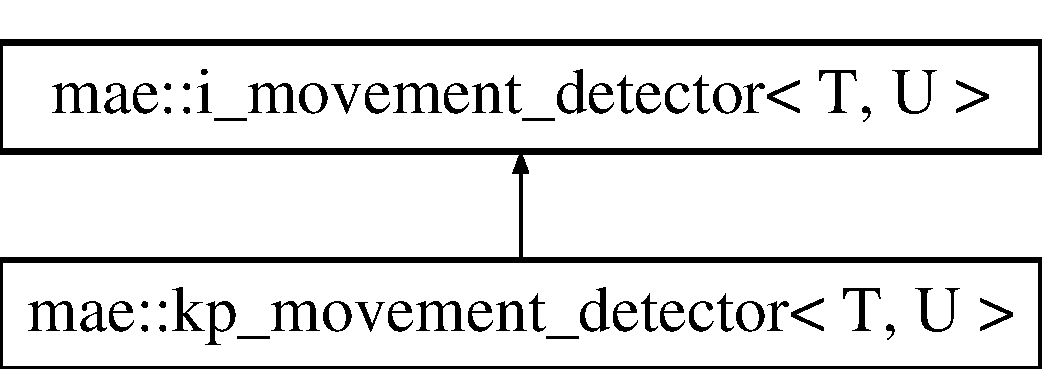
\includegraphics[height=2.000000cm]{classmae_1_1i__movement__detector}
\end{center}
\end{figure}
\subsection*{Public Member Functions}
\begin{DoxyCompactItemize}
\item 
virtual std\-::shared\-\_\-ptr$<$ U $>$ \hyperlink{classmae_1_1i__movement__detector_aa3b5c4491ce4f11ef6a116ba05084f1a}{detect\-\_\-movement} (uint64\-\_\-t timestamp, double framerate, std\-::shared\-\_\-ptr$<$ T $>$ skeleton, std\-::vector$<$ \hyperlink{classmae_1_1bone}{bone} $>$ body\-\_\-parts)=0
\item 
virtual void \hyperlink{classmae_1_1i__movement__detector_a96a923c5bab2dbed81daf4cadc885497}{set\-\_\-buffer} (int size)=0
\item 
virtual void \hyperlink{classmae_1_1i__movement__detector_a73db186e7b58daa0923f00b285671172}{clear\-\_\-buffer} ()=0
\item 
virtual void \hyperlink{classmae_1_1i__movement__detector_af6724fa4c8ddb032411825168e4b02d4}{add\-\_\-listener} (std\-::shared\-\_\-ptr$<$ \hyperlink{classmae_1_1i__pose__listener}{i\-\_\-pose\-\_\-listener} $>$ listener)=0
\item 
virtual void \hyperlink{classmae_1_1i__movement__detector_a88d965f2b8d04e0681e2e7cd42bd7331}{remove\-\_\-listener} (std\-::shared\-\_\-ptr$<$ \hyperlink{classmae_1_1i__pose__listener}{i\-\_\-pose\-\_\-listener} $>$ listener)=0
\item 
virtual void \hyperlink{classmae_1_1i__movement__detector_a56a36a8a427feb34f970b9e259a1150f}{clear\-\_\-listeners} ()=0
\item 
virtual void \hyperlink{classmae_1_1i__movement__detector_aebdc95347866bc2bc6b793383585fe2f}{notify\-\_\-listeners} (uint64\-\_\-t timestamp, std\-::shared\-\_\-ptr$<$ \hyperlink{classmae_1_1general__pose}{general\-\_\-pose} $>$ pose)=0
\item 
virtual std\-::shared\-\_\-ptr\\*
$<$ \hyperlink{classmae_1_1general__pose}{general\-\_\-pose} $>$ \hyperlink{classmae_1_1i__movement__detector_a67db28512cb293217156fd8611322d75}{get\-\_\-current\-\_\-pose} () const =0
\end{DoxyCompactItemize}


\subsection{Member Function Documentation}
\hypertarget{classmae_1_1i__movement__detector_af6724fa4c8ddb032411825168e4b02d4}{\index{mae\-::i\-\_\-movement\-\_\-detector@{mae\-::i\-\_\-movement\-\_\-detector}!add\-\_\-listener@{add\-\_\-listener}}
\index{add\-\_\-listener@{add\-\_\-listener}!mae::i_movement_detector@{mae\-::i\-\_\-movement\-\_\-detector}}
\subsubsection[{add\-\_\-listener}]{\setlength{\rightskip}{0pt plus 5cm}template$<$typename T , typename U $>$ virtual void {\bf mae\-::i\-\_\-movement\-\_\-detector}$<$ T, U $>$\-::add\-\_\-listener (
\begin{DoxyParamCaption}
\item[{std\-::shared\-\_\-ptr$<$ {\bf i\-\_\-pose\-\_\-listener} $>$}]{listener}
\end{DoxyParamCaption}
)\hspace{0.3cm}{\ttfamily [pure virtual]}}}\label{classmae_1_1i__movement__detector_af6724fa4c8ddb032411825168e4b02d4}
Adds a pose listener to the detector. The listeners are invoked whenever a pose is fully detected (each frame).


\begin{DoxyParams}{Parameters}
{\em listener} & The listener to be added. \\
\hline
\end{DoxyParams}


Implemented in \hyperlink{classmae_1_1kp__movement__detector_a53f506b2d9c5bb759908a125af33f97d}{mae\-::kp\-\_\-movement\-\_\-detector$<$ T, U $>$}.

\hypertarget{classmae_1_1i__movement__detector_a73db186e7b58daa0923f00b285671172}{\index{mae\-::i\-\_\-movement\-\_\-detector@{mae\-::i\-\_\-movement\-\_\-detector}!clear\-\_\-buffer@{clear\-\_\-buffer}}
\index{clear\-\_\-buffer@{clear\-\_\-buffer}!mae::i_movement_detector@{mae\-::i\-\_\-movement\-\_\-detector}}
\subsubsection[{clear\-\_\-buffer}]{\setlength{\rightskip}{0pt plus 5cm}template$<$typename T , typename U $>$ virtual void {\bf mae\-::i\-\_\-movement\-\_\-detector}$<$ T, U $>$\-::clear\-\_\-buffer (
\begin{DoxyParamCaption}
{}
\end{DoxyParamCaption}
)\hspace{0.3cm}{\ttfamily [pure virtual]}}}\label{classmae_1_1i__movement__detector_a73db186e7b58daa0923f00b285671172}
Clears the buffer used to store the data. 

Implemented in \hyperlink{classmae_1_1kp__movement__detector_a8fec5ae9e1f209fdcbeba3f86b5c3059}{mae\-::kp\-\_\-movement\-\_\-detector$<$ T, U $>$}.

\hypertarget{classmae_1_1i__movement__detector_a56a36a8a427feb34f970b9e259a1150f}{\index{mae\-::i\-\_\-movement\-\_\-detector@{mae\-::i\-\_\-movement\-\_\-detector}!clear\-\_\-listeners@{clear\-\_\-listeners}}
\index{clear\-\_\-listeners@{clear\-\_\-listeners}!mae::i_movement_detector@{mae\-::i\-\_\-movement\-\_\-detector}}
\subsubsection[{clear\-\_\-listeners}]{\setlength{\rightskip}{0pt plus 5cm}template$<$typename T , typename U $>$ virtual void {\bf mae\-::i\-\_\-movement\-\_\-detector}$<$ T, U $>$\-::clear\-\_\-listeners (
\begin{DoxyParamCaption}
{}
\end{DoxyParamCaption}
)\hspace{0.3cm}{\ttfamily [pure virtual]}}}\label{classmae_1_1i__movement__detector_a56a36a8a427feb34f970b9e259a1150f}
Clears all listeners, which means removing them from the detector. 

Implemented in \hyperlink{classmae_1_1kp__movement__detector_a5333495e30be2b0d6205cd8266d2156d}{mae\-::kp\-\_\-movement\-\_\-detector$<$ T, U $>$}.

\hypertarget{classmae_1_1i__movement__detector_aa3b5c4491ce4f11ef6a116ba05084f1a}{\index{mae\-::i\-\_\-movement\-\_\-detector@{mae\-::i\-\_\-movement\-\_\-detector}!detect\-\_\-movement@{detect\-\_\-movement}}
\index{detect\-\_\-movement@{detect\-\_\-movement}!mae::i_movement_detector@{mae\-::i\-\_\-movement\-\_\-detector}}
\subsubsection[{detect\-\_\-movement}]{\setlength{\rightskip}{0pt plus 5cm}template$<$typename T , typename U $>$ virtual std\-::shared\-\_\-ptr$<$U$>$ {\bf mae\-::i\-\_\-movement\-\_\-detector}$<$ T, U $>$\-::detect\-\_\-movement (
\begin{DoxyParamCaption}
\item[{uint64\-\_\-t}]{timestamp, }
\item[{double}]{framerate, }
\item[{std\-::shared\-\_\-ptr$<$ T $>$}]{skeleton, }
\item[{std\-::vector$<$ {\bf bone} $>$}]{body\-\_\-parts}
\end{DoxyParamCaption}
)\hspace{0.3cm}{\ttfamily [pure virtual]}}}\label{classmae_1_1i__movement__detector_aa3b5c4491ce4f11ef6a116ba05084f1a}
Detects movement in the streamed skeleton sequence for the given body parts. Therefore, a buffer is required and the whole movement sequence for the buffer is returned.


\begin{DoxyParams}{Parameters}
{\em timestamp} & The timestamp of the current frame as provided by the user. It is not save to rely on this value. \\
\hline
{\em framerate} & The framerate to be applied. The framerate does not change. \\
\hline
{\em skeleton} & The skeleton data. \\
\hline
{\em body\-\_\-parts} & The addressed body parts. \\
\hline
\end{DoxyParams}
\begin{DoxyReturn}{Returns}
The detected movement sequence. 
\end{DoxyReturn}


Implemented in \hyperlink{classmae_1_1kp__movement__detector_a05c206df200417ea7680eb9d8a5cb6b0}{mae\-::kp\-\_\-movement\-\_\-detector$<$ T, U $>$}.

\hypertarget{classmae_1_1i__movement__detector_a67db28512cb293217156fd8611322d75}{\index{mae\-::i\-\_\-movement\-\_\-detector@{mae\-::i\-\_\-movement\-\_\-detector}!get\-\_\-current\-\_\-pose@{get\-\_\-current\-\_\-pose}}
\index{get\-\_\-current\-\_\-pose@{get\-\_\-current\-\_\-pose}!mae::i_movement_detector@{mae\-::i\-\_\-movement\-\_\-detector}}
\subsubsection[{get\-\_\-current\-\_\-pose}]{\setlength{\rightskip}{0pt plus 5cm}template$<$typename T , typename U $>$ virtual std\-::shared\-\_\-ptr$<${\bf general\-\_\-pose}$>$ {\bf mae\-::i\-\_\-movement\-\_\-detector}$<$ T, U $>$\-::get\-\_\-current\-\_\-pose (
\begin{DoxyParamCaption}
{}
\end{DoxyParamCaption}
) const\hspace{0.3cm}{\ttfamily [pure virtual]}}}\label{classmae_1_1i__movement__detector_a67db28512cb293217156fd8611322d75}
Returns the last processed pose.

\begin{DoxyReturn}{Returns}
The last processed pose. 
\end{DoxyReturn}


Implemented in \hyperlink{classmae_1_1kp__movement__detector_a0cf1bb06689f4a983daed5a5fc1935c6}{mae\-::kp\-\_\-movement\-\_\-detector$<$ T, U $>$}.

\hypertarget{classmae_1_1i__movement__detector_aebdc95347866bc2bc6b793383585fe2f}{\index{mae\-::i\-\_\-movement\-\_\-detector@{mae\-::i\-\_\-movement\-\_\-detector}!notify\-\_\-listeners@{notify\-\_\-listeners}}
\index{notify\-\_\-listeners@{notify\-\_\-listeners}!mae::i_movement_detector@{mae\-::i\-\_\-movement\-\_\-detector}}
\subsubsection[{notify\-\_\-listeners}]{\setlength{\rightskip}{0pt plus 5cm}template$<$typename T , typename U $>$ virtual void {\bf mae\-::i\-\_\-movement\-\_\-detector}$<$ T, U $>$\-::notify\-\_\-listeners (
\begin{DoxyParamCaption}
\item[{uint64\-\_\-t}]{timestamp, }
\item[{std\-::shared\-\_\-ptr$<$ {\bf general\-\_\-pose} $>$}]{pose}
\end{DoxyParamCaption}
)\hspace{0.3cm}{\ttfamily [pure virtual]}}}\label{classmae_1_1i__movement__detector_aebdc95347866bc2bc6b793383585fe2f}
Notifies all listeners on the detection of a new pose.


\begin{DoxyParams}{Parameters}
{\em timestamp} & \\
\hline
{\em pose} & \\
\hline
\end{DoxyParams}


Implemented in \hyperlink{classmae_1_1kp__movement__detector_acdc61f7edc7fdaadb5134e6cabd04612}{mae\-::kp\-\_\-movement\-\_\-detector$<$ T, U $>$}.

\hypertarget{classmae_1_1i__movement__detector_a88d965f2b8d04e0681e2e7cd42bd7331}{\index{mae\-::i\-\_\-movement\-\_\-detector@{mae\-::i\-\_\-movement\-\_\-detector}!remove\-\_\-listener@{remove\-\_\-listener}}
\index{remove\-\_\-listener@{remove\-\_\-listener}!mae::i_movement_detector@{mae\-::i\-\_\-movement\-\_\-detector}}
\subsubsection[{remove\-\_\-listener}]{\setlength{\rightskip}{0pt plus 5cm}template$<$typename T , typename U $>$ virtual void {\bf mae\-::i\-\_\-movement\-\_\-detector}$<$ T, U $>$\-::remove\-\_\-listener (
\begin{DoxyParamCaption}
\item[{std\-::shared\-\_\-ptr$<$ {\bf i\-\_\-pose\-\_\-listener} $>$}]{listener}
\end{DoxyParamCaption}
)\hspace{0.3cm}{\ttfamily [pure virtual]}}}\label{classmae_1_1i__movement__detector_a88d965f2b8d04e0681e2e7cd42bd7331}
Removes the listener from the detector.


\begin{DoxyParams}{Parameters}
{\em listener} & The listener to be removed. \\
\hline
\end{DoxyParams}


Implemented in \hyperlink{classmae_1_1kp__movement__detector_a6c93647920874e88c5b6293617cfdca2}{mae\-::kp\-\_\-movement\-\_\-detector$<$ T, U $>$}.

\hypertarget{classmae_1_1i__movement__detector_a96a923c5bab2dbed81daf4cadc885497}{\index{mae\-::i\-\_\-movement\-\_\-detector@{mae\-::i\-\_\-movement\-\_\-detector}!set\-\_\-buffer@{set\-\_\-buffer}}
\index{set\-\_\-buffer@{set\-\_\-buffer}!mae::i_movement_detector@{mae\-::i\-\_\-movement\-\_\-detector}}
\subsubsection[{set\-\_\-buffer}]{\setlength{\rightskip}{0pt plus 5cm}template$<$typename T , typename U $>$ virtual void {\bf mae\-::i\-\_\-movement\-\_\-detector}$<$ T, U $>$\-::set\-\_\-buffer (
\begin{DoxyParamCaption}
\item[{int}]{size}
\end{DoxyParamCaption}
)\hspace{0.3cm}{\ttfamily [pure virtual]}}}\label{classmae_1_1i__movement__detector_a96a923c5bab2dbed81daf4cadc885497}
Updates the buffer size used to store the skeleton data.


\begin{DoxyParams}{Parameters}
{\em size} & The buffer size. \\
\hline
\end{DoxyParams}


Implemented in \hyperlink{classmae_1_1kp__movement__detector_a673ed3ff4f7a5cd8a02cdbe254a4508e}{mae\-::kp\-\_\-movement\-\_\-detector$<$ T, U $>$}.



The documentation for this class was generated from the following file\-:\begin{DoxyCompactItemize}
\item 
src/mae/i\-\_\-movement\-\_\-detector.\-hpp\end{DoxyCompactItemize}

\hypertarget{classmae_1_1fl_1_1laban_1_1ps_1_1i__part}{\section{mae\-:\-:fl\-:\-:laban\-:\-:ps\-:\-:i\-\_\-part Class Reference}
\label{classmae_1_1fl_1_1laban_1_1ps_1_1i__part}\index{mae\-::fl\-::laban\-::ps\-::i\-\_\-part@{mae\-::fl\-::laban\-::ps\-::i\-\_\-part}}
}
Inheritance diagram for mae\-:\-:fl\-:\-:laban\-:\-:ps\-:\-:i\-\_\-part\-:\begin{figure}[H]
\begin{center}
\leavevmode
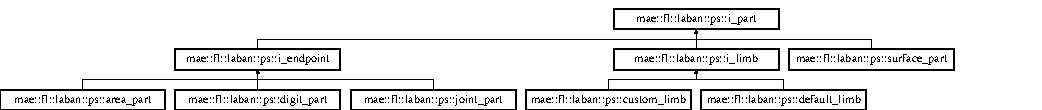
\includegraphics[height=1.473684cm]{classmae_1_1fl_1_1laban_1_1ps_1_1i__part}
\end{center}
\end{figure}
\subsection*{Public Member Functions}
\begin{DoxyCompactItemize}
\item 
virtual std\-::string \hyperlink{classmae_1_1fl_1_1laban_1_1ps_1_1i__part_a704c07899099cdf53beb9187f23b7874}{xml} (unsigned int indent=0, std\-::string namesp=\char`\"{}\char`\"{}) const =0
\item 
virtual std\-::string \hyperlink{classmae_1_1fl_1_1laban_1_1ps_1_1i__part_a78227d5ecd87655a7a9454c68f470368}{svg} (std\-::string identifier, double posx, double posy, double width, double height, bool left=false) const =0
\item 
virtual bool \hyperlink{classmae_1_1fl_1_1laban_1_1ps_1_1i__part_ad43f6b88cb409ac26342db51606ea1e1}{equals} (std\-::shared\-\_\-ptr$<$ \hyperlink{classmae_1_1fl_1_1laban_1_1ps_1_1i__part}{i\-\_\-part} $>$ a) const =0
\end{DoxyCompactItemize}


\subsection{Member Function Documentation}
\hypertarget{classmae_1_1fl_1_1laban_1_1ps_1_1i__part_ad43f6b88cb409ac26342db51606ea1e1}{\index{mae\-::fl\-::laban\-::ps\-::i\-\_\-part@{mae\-::fl\-::laban\-::ps\-::i\-\_\-part}!equals@{equals}}
\index{equals@{equals}!mae::fl::laban::ps::i_part@{mae\-::fl\-::laban\-::ps\-::i\-\_\-part}}
\subsubsection[{equals}]{\setlength{\rightskip}{0pt plus 5cm}virtual bool mae\-::fl\-::laban\-::ps\-::i\-\_\-part\-::equals (
\begin{DoxyParamCaption}
\item[{std\-::shared\-\_\-ptr$<$ {\bf i\-\_\-part} $>$}]{a}
\end{DoxyParamCaption}
) const\hspace{0.3cm}{\ttfamily [pure virtual]}}}\label{classmae_1_1fl_1_1laban_1_1ps_1_1i__part_ad43f6b88cb409ac26342db51606ea1e1}
Returns true if elements are equal.


\begin{DoxyParams}{Parameters}
{\em a} & The element to be compared to. \\
\hline
\end{DoxyParams}
\begin{DoxyReturn}{Returns}
True if equal. 
\end{DoxyReturn}


Implemented in \hyperlink{classmae_1_1fl_1_1laban_1_1ps_1_1digit__part_a6bcdd921e55c60908e827534d4957c4d}{mae\-::fl\-::laban\-::ps\-::digit\-\_\-part}, \hyperlink{classmae_1_1fl_1_1laban_1_1ps_1_1surface__part_a1ca1e44626d00dd7647927bafd86c266}{mae\-::fl\-::laban\-::ps\-::surface\-\_\-part}, \hyperlink{classmae_1_1fl_1_1laban_1_1ps_1_1custom__limb_aea87a1c04a4a8fde3ef80862690b0318}{mae\-::fl\-::laban\-::ps\-::custom\-\_\-limb}, \hyperlink{classmae_1_1fl_1_1laban_1_1ps_1_1area__part_aa223417cb9c21426014d0099f9fad72b}{mae\-::fl\-::laban\-::ps\-::area\-\_\-part}, \hyperlink{classmae_1_1fl_1_1laban_1_1ps_1_1joint__part_a1de75536e4a12e1435e0ec3c4f2edbad}{mae\-::fl\-::laban\-::ps\-::joint\-\_\-part}, \hyperlink{classmae_1_1fl_1_1laban_1_1ps_1_1default__limb_a9bdae13195e31e15c5511dcf04786aae}{mae\-::fl\-::laban\-::ps\-::default\-\_\-limb}, \hyperlink{classmae_1_1fl_1_1laban_1_1ps_1_1i__endpoint_abc675b07d3ce69fbec362b2e792a1e06}{mae\-::fl\-::laban\-::ps\-::i\-\_\-endpoint}, and \hyperlink{classmae_1_1fl_1_1laban_1_1ps_1_1i__limb_aa46cb4b952cc2a8692f3f32895a28041}{mae\-::fl\-::laban\-::ps\-::i\-\_\-limb}.

\hypertarget{classmae_1_1fl_1_1laban_1_1ps_1_1i__part_a78227d5ecd87655a7a9454c68f470368}{\index{mae\-::fl\-::laban\-::ps\-::i\-\_\-part@{mae\-::fl\-::laban\-::ps\-::i\-\_\-part}!svg@{svg}}
\index{svg@{svg}!mae::fl::laban::ps::i_part@{mae\-::fl\-::laban\-::ps\-::i\-\_\-part}}
\subsubsection[{svg}]{\setlength{\rightskip}{0pt plus 5cm}virtual std\-::string mae\-::fl\-::laban\-::ps\-::i\-\_\-part\-::svg (
\begin{DoxyParamCaption}
\item[{std\-::string}]{identifier, }
\item[{double}]{posx, }
\item[{double}]{posy, }
\item[{double}]{width, }
\item[{double}]{height, }
\item[{bool}]{left = {\ttfamily false}}
\end{DoxyParamCaption}
) const\hspace{0.3cm}{\ttfamily [pure virtual]}}}\label{classmae_1_1fl_1_1laban_1_1ps_1_1i__part_a78227d5ecd87655a7a9454c68f470368}
Returns the S\-V\-G representation for this symbol.


\begin{DoxyParams}{Parameters}
{\em posx} & The x position. \\
\hline
{\em posy} & The y position. \\
\hline
{\em width} & The width. \\
\hline
{\em height} & The height. \\
\hline
\end{DoxyParams}
\begin{DoxyReturn}{Returns}
The S\-V\-G. 
\end{DoxyReturn}


Implemented in \hyperlink{classmae_1_1fl_1_1laban_1_1ps_1_1digit__part_a4f9204b03aaf808940d32d1b6a3ea325}{mae\-::fl\-::laban\-::ps\-::digit\-\_\-part}, \hyperlink{classmae_1_1fl_1_1laban_1_1ps_1_1surface__part_a91102bf6d87a18afa19ace304c4607e0}{mae\-::fl\-::laban\-::ps\-::surface\-\_\-part}, \hyperlink{classmae_1_1fl_1_1laban_1_1ps_1_1custom__limb_aa002dfaca3b1f073f67a85572095b504}{mae\-::fl\-::laban\-::ps\-::custom\-\_\-limb}, \hyperlink{classmae_1_1fl_1_1laban_1_1ps_1_1default__limb_a489743d2be319dec0e05049b3c09db1e}{mae\-::fl\-::laban\-::ps\-::default\-\_\-limb}, \hyperlink{classmae_1_1fl_1_1laban_1_1ps_1_1area__part_ad28ba26a5e96db2f23f07f974633fdf7}{mae\-::fl\-::laban\-::ps\-::area\-\_\-part}, and \hyperlink{classmae_1_1fl_1_1laban_1_1ps_1_1joint__part_af8e8475612c99842a6b6a18964168592}{mae\-::fl\-::laban\-::ps\-::joint\-\_\-part}.

\hypertarget{classmae_1_1fl_1_1laban_1_1ps_1_1i__part_a704c07899099cdf53beb9187f23b7874}{\index{mae\-::fl\-::laban\-::ps\-::i\-\_\-part@{mae\-::fl\-::laban\-::ps\-::i\-\_\-part}!xml@{xml}}
\index{xml@{xml}!mae::fl::laban::ps::i_part@{mae\-::fl\-::laban\-::ps\-::i\-\_\-part}}
\subsubsection[{xml}]{\setlength{\rightskip}{0pt plus 5cm}virtual std\-::string mae\-::fl\-::laban\-::ps\-::i\-\_\-part\-::xml (
\begin{DoxyParamCaption}
\item[{unsigned int}]{indent = {\ttfamily 0}, }
\item[{std\-::string}]{namesp = {\ttfamily \char`\"{}\char`\"{}}}
\end{DoxyParamCaption}
) const\hspace{0.3cm}{\ttfamily [pure virtual]}}}\label{classmae_1_1fl_1_1laban_1_1ps_1_1i__part_a704c07899099cdf53beb9187f23b7874}
Returns the X\-M\-L representation for this element.


\begin{DoxyParams}{Parameters}
{\em indent} & The applied indent. \\
\hline
{\em namesp} & The prefixed X\-M\-L namespace.\\
\hline
\end{DoxyParams}
\begin{DoxyReturn}{Returns}
The X\-M\-L string. 
\end{DoxyReturn}


Implemented in \hyperlink{classmae_1_1fl_1_1laban_1_1ps_1_1digit__part_a51e9b056b0d57310e1423efbf8ebec48}{mae\-::fl\-::laban\-::ps\-::digit\-\_\-part}, \hyperlink{classmae_1_1fl_1_1laban_1_1ps_1_1surface__part_a1853ed550de38dbc7b1b38b6ff676904}{mae\-::fl\-::laban\-::ps\-::surface\-\_\-part}, \hyperlink{classmae_1_1fl_1_1laban_1_1ps_1_1custom__limb_a2622dd693ce2f662a4802025b42f1e64}{mae\-::fl\-::laban\-::ps\-::custom\-\_\-limb}, \hyperlink{classmae_1_1fl_1_1laban_1_1ps_1_1default__limb_a1d266ba068ce557431a90476b0ce3a82}{mae\-::fl\-::laban\-::ps\-::default\-\_\-limb}, \hyperlink{classmae_1_1fl_1_1laban_1_1ps_1_1area__part_a3ffd61d8cba76a5312a737a40dccb4ec}{mae\-::fl\-::laban\-::ps\-::area\-\_\-part}, \hyperlink{classmae_1_1fl_1_1laban_1_1ps_1_1joint__part_a3054936a94c43d4cb3cb21745234e2cf}{mae\-::fl\-::laban\-::ps\-::joint\-\_\-part}, \hyperlink{classmae_1_1fl_1_1laban_1_1ps_1_1i__endpoint_a1af7dbd05400cbdd7f9f45ef75dd38d6}{mae\-::fl\-::laban\-::ps\-::i\-\_\-endpoint}, and \hyperlink{classmae_1_1fl_1_1laban_1_1ps_1_1i__limb_a7a5c3ca32936748a1e60fdab1d29b1c9}{mae\-::fl\-::laban\-::ps\-::i\-\_\-limb}.



The documentation for this class was generated from the following file\-:\begin{DoxyCompactItemize}
\item 
src/mae/fl/laban/ps/i\-\_\-part.\-hpp\end{DoxyCompactItemize}

\hypertarget{classmae_1_1i__pose__detector}{\section{mae\-:\-:i\-\_\-pose\-\_\-detector$<$ T $>$ Class Template Reference}
\label{classmae_1_1i__pose__detector}\index{mae\-::i\-\_\-pose\-\_\-detector$<$ T $>$@{mae\-::i\-\_\-pose\-\_\-detector$<$ T $>$}}
}
\subsection*{Public Member Functions}
\begin{DoxyCompactItemize}
\item 
virtual std\-::shared\-\_\-ptr\\*
$<$ \hyperlink{classmae_1_1general__pose}{general\-\_\-pose} $>$ \hyperlink{classmae_1_1i__pose__detector_aebc5f509e4ac79b81d248301f229d127}{pose} (double framerate, std\-::shared\-\_\-ptr$<$ T $>$ skeleton, std\-::vector$<$ \hyperlink{classmae_1_1bone}{bone} $>$ body\-\_\-parts, std\-::shared\-\_\-ptr$<$ \hyperlink{classmae_1_1general__pose}{general\-\_\-pose} $>$ previous\-\_\-pose)=0
\end{DoxyCompactItemize}


\subsection{Member Function Documentation}
\hypertarget{classmae_1_1i__pose__detector_aebc5f509e4ac79b81d248301f229d127}{\index{mae\-::i\-\_\-pose\-\_\-detector@{mae\-::i\-\_\-pose\-\_\-detector}!pose@{pose}}
\index{pose@{pose}!mae::i_pose_detector@{mae\-::i\-\_\-pose\-\_\-detector}}
\subsubsection[{pose}]{\setlength{\rightskip}{0pt plus 5cm}template$<$typename T$>$ virtual std\-::shared\-\_\-ptr$<${\bf general\-\_\-pose}$>$ {\bf mae\-::i\-\_\-pose\-\_\-detector}$<$ T $>$\-::pose (
\begin{DoxyParamCaption}
\item[{double}]{framerate, }
\item[{std\-::shared\-\_\-ptr$<$ T $>$}]{skeleton, }
\item[{std\-::vector$<$ {\bf bone} $>$}]{body\-\_\-parts, }
\item[{std\-::shared\-\_\-ptr$<$ {\bf general\-\_\-pose} $>$}]{previous\-\_\-pose}
\end{DoxyParamCaption}
)\hspace{0.3cm}{\ttfamily [pure virtual]}}}\label{classmae_1_1i__pose__detector_aebc5f509e4ac79b81d248301f229d127}
Processes the skeleton in order to return the pose for each body part.


\begin{DoxyParams}{Parameters}
{\em framerate} & The framerate. \\
\hline
{\em skeleton} & The skeleton. \\
\hline
{\em body\-\_\-parts} & The processed body parts. \\
\hline
{\em previous\-\_\-pose} & The previous pose that can be used for hysteresis. \\
\hline
\end{DoxyParams}
\begin{DoxyReturn}{Returns}
The pose. 
\end{DoxyReturn}


The documentation for this class was generated from the following file\-:\begin{DoxyCompactItemize}
\item 
src/mae/i\-\_\-pose\-\_\-detector.\-hpp\end{DoxyCompactItemize}

\hypertarget{classmae_1_1i__pose__listener}{\section{mae\-:\-:i\-\_\-pose\-\_\-listener Class Reference}
\label{classmae_1_1i__pose__listener}\index{mae\-::i\-\_\-pose\-\_\-listener@{mae\-::i\-\_\-pose\-\_\-listener}}
}


{\ttfamily \#include $<$i\-\_\-pose\-\_\-listener.\-hpp$>$}

Inheritance diagram for mae\-:\-:i\-\_\-pose\-\_\-listener\-:\begin{figure}[H]
\begin{center}
\leavevmode
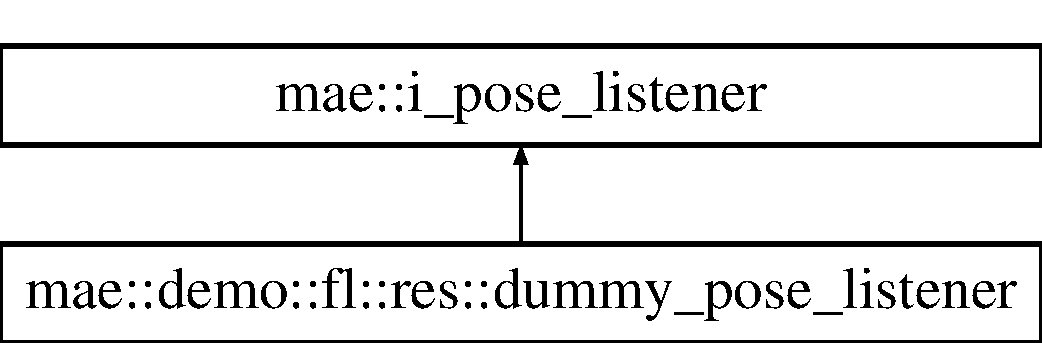
\includegraphics[height=2.000000cm]{classmae_1_1i__pose__listener}
\end{center}
\end{figure}
\subsection*{Public Member Functions}
\begin{DoxyCompactItemize}
\item 
virtual void \hyperlink{classmae_1_1i__pose__listener_a1b7584ba2ad90a2b862d779cb3cba6f5}{on\-\_\-pose} (long timestamp, std\-::shared\-\_\-ptr$<$ \hyperlink{classmae_1_1general__pose}{general\-\_\-pose} $>$ pose)=0
\end{DoxyCompactItemize}


\subsection{Detailed Description}
Listener for poses. In notified each frame after the pose quantization. 

\subsection{Member Function Documentation}
\hypertarget{classmae_1_1i__pose__listener_a1b7584ba2ad90a2b862d779cb3cba6f5}{\index{mae\-::i\-\_\-pose\-\_\-listener@{mae\-::i\-\_\-pose\-\_\-listener}!on\-\_\-pose@{on\-\_\-pose}}
\index{on\-\_\-pose@{on\-\_\-pose}!mae::i_pose_listener@{mae\-::i\-\_\-pose\-\_\-listener}}
\subsubsection[{on\-\_\-pose}]{\setlength{\rightskip}{0pt plus 5cm}virtual void mae\-::i\-\_\-pose\-\_\-listener\-::on\-\_\-pose (
\begin{DoxyParamCaption}
\item[{long}]{timestamp, }
\item[{std\-::shared\-\_\-ptr$<$ {\bf general\-\_\-pose} $>$}]{pose}
\end{DoxyParamCaption}
)\hspace{0.3cm}{\ttfamily [pure virtual]}}}\label{classmae_1_1i__pose__listener_a1b7584ba2ad90a2b862d779cb3cba6f5}
Is invoked each time a pose was quantized (which occurs on every frame).


\begin{DoxyParams}{Parameters}
{\em timestamp} & The associated timestamp. \\
\hline
{\em pose} & The quantized pose. \\
\hline
\end{DoxyParams}


Implemented in \hyperlink{classmae_1_1demo_1_1fl_1_1res_1_1dummy__pose__listener_adc5d9098a8e94040c4d3ae633c075423}{mae\-::demo\-::fl\-::res\-::dummy\-\_\-pose\-\_\-listener}.



The documentation for this class was generated from the following file\-:\begin{DoxyCompactItemize}
\item 
src/mae/i\-\_\-pose\-\_\-listener.\-hpp\end{DoxyCompactItemize}

\hypertarget{classmae_1_1fl_1_1laban_1_1ps_1_1i__pre__sign}{\section{mae\-:\-:fl\-:\-:laban\-:\-:ps\-:\-:i\-\_\-pre\-\_\-sign Class Reference}
\label{classmae_1_1fl_1_1laban_1_1ps_1_1i__pre__sign}\index{mae\-::fl\-::laban\-::ps\-::i\-\_\-pre\-\_\-sign@{mae\-::fl\-::laban\-::ps\-::i\-\_\-pre\-\_\-sign}}
}
Inheritance diagram for mae\-:\-:fl\-:\-:laban\-:\-:ps\-:\-:i\-\_\-pre\-\_\-sign\-:\begin{figure}[H]
\begin{center}
\leavevmode
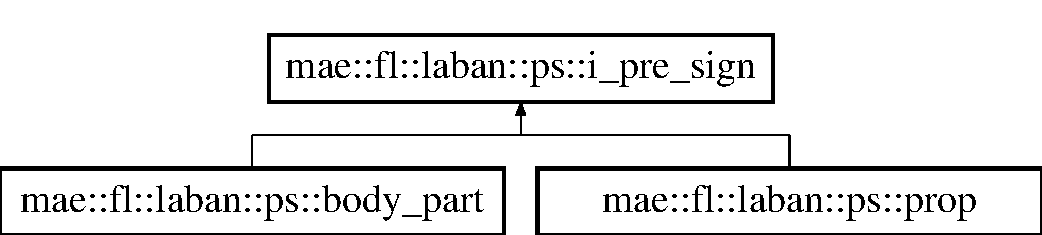
\includegraphics[height=2.000000cm]{classmae_1_1fl_1_1laban_1_1ps_1_1i__pre__sign}
\end{center}
\end{figure}
\subsection*{Public Member Functions}
\begin{DoxyCompactItemize}
\item 
virtual std\-::string \hyperlink{classmae_1_1fl_1_1laban_1_1ps_1_1i__pre__sign_a428b08efc67bb293f0fc8b41ce40215f}{xml} (unsigned int indent=0, std\-::string namesp=\char`\"{}\char`\"{}) const =0
\item 
virtual std\-::string \hyperlink{classmae_1_1fl_1_1laban_1_1ps_1_1i__pre__sign_a3caa95eb1c8637f531812afe1b78bbf4}{svg} (std\-::string identifier, double posx, double posy, double width, double height, bool left=false) const =0
\item 
virtual bool \hyperlink{classmae_1_1fl_1_1laban_1_1ps_1_1i__pre__sign_a8e3342fe33b6bd050d613330da30213d}{equals} (std\-::shared\-\_\-ptr$<$ \hyperlink{classmae_1_1fl_1_1laban_1_1ps_1_1i__pre__sign}{i\-\_\-pre\-\_\-sign} $>$ a) const =0
\end{DoxyCompactItemize}


\subsection{Member Function Documentation}
\hypertarget{classmae_1_1fl_1_1laban_1_1ps_1_1i__pre__sign_a8e3342fe33b6bd050d613330da30213d}{\index{mae\-::fl\-::laban\-::ps\-::i\-\_\-pre\-\_\-sign@{mae\-::fl\-::laban\-::ps\-::i\-\_\-pre\-\_\-sign}!equals@{equals}}
\index{equals@{equals}!mae::fl::laban::ps::i_pre_sign@{mae\-::fl\-::laban\-::ps\-::i\-\_\-pre\-\_\-sign}}
\subsubsection[{equals}]{\setlength{\rightskip}{0pt plus 5cm}virtual bool mae\-::fl\-::laban\-::ps\-::i\-\_\-pre\-\_\-sign\-::equals (
\begin{DoxyParamCaption}
\item[{std\-::shared\-\_\-ptr$<$ {\bf i\-\_\-pre\-\_\-sign} $>$}]{a}
\end{DoxyParamCaption}
) const\hspace{0.3cm}{\ttfamily [pure virtual]}}}\label{classmae_1_1fl_1_1laban_1_1ps_1_1i__pre__sign_a8e3342fe33b6bd050d613330da30213d}
Returns true if elements are equal.


\begin{DoxyParams}{Parameters}
{\em a} & The element to be compared to. \\
\hline
\end{DoxyParams}
\begin{DoxyReturn}{Returns}
True if equal. 
\end{DoxyReturn}


Implemented in \hyperlink{classmae_1_1fl_1_1laban_1_1ps_1_1body__part_abc74bc42375b203522754607f85851c4}{mae\-::fl\-::laban\-::ps\-::body\-\_\-part}, and \hyperlink{classmae_1_1fl_1_1laban_1_1ps_1_1prop_a03b8c4bfa1731767fe0c868555c17c1b}{mae\-::fl\-::laban\-::ps\-::prop}.

\hypertarget{classmae_1_1fl_1_1laban_1_1ps_1_1i__pre__sign_a3caa95eb1c8637f531812afe1b78bbf4}{\index{mae\-::fl\-::laban\-::ps\-::i\-\_\-pre\-\_\-sign@{mae\-::fl\-::laban\-::ps\-::i\-\_\-pre\-\_\-sign}!svg@{svg}}
\index{svg@{svg}!mae::fl::laban::ps::i_pre_sign@{mae\-::fl\-::laban\-::ps\-::i\-\_\-pre\-\_\-sign}}
\subsubsection[{svg}]{\setlength{\rightskip}{0pt plus 5cm}virtual std\-::string mae\-::fl\-::laban\-::ps\-::i\-\_\-pre\-\_\-sign\-::svg (
\begin{DoxyParamCaption}
\item[{std\-::string}]{identifier, }
\item[{double}]{posx, }
\item[{double}]{posy, }
\item[{double}]{width, }
\item[{double}]{height, }
\item[{bool}]{left = {\ttfamily false}}
\end{DoxyParamCaption}
) const\hspace{0.3cm}{\ttfamily [pure virtual]}}}\label{classmae_1_1fl_1_1laban_1_1ps_1_1i__pre__sign_a3caa95eb1c8637f531812afe1b78bbf4}
Returns the S\-V\-G representation for this symbol.


\begin{DoxyParams}{Parameters}
{\em posx} & The x position. \\
\hline
{\em posy} & The y position. \\
\hline
{\em width} & The width. \\
\hline
{\em height} & The height. \\
\hline
\end{DoxyParams}
\begin{DoxyReturn}{Returns}
The S\-V\-G. 
\end{DoxyReturn}


Implemented in \hyperlink{classmae_1_1fl_1_1laban_1_1ps_1_1body__part_aad8376f76f0cc424da8569ada4579c9a}{mae\-::fl\-::laban\-::ps\-::body\-\_\-part}, and \hyperlink{classmae_1_1fl_1_1laban_1_1ps_1_1prop_ae0439113058f4ed15bc3826f3e93e6d9}{mae\-::fl\-::laban\-::ps\-::prop}.

\hypertarget{classmae_1_1fl_1_1laban_1_1ps_1_1i__pre__sign_a428b08efc67bb293f0fc8b41ce40215f}{\index{mae\-::fl\-::laban\-::ps\-::i\-\_\-pre\-\_\-sign@{mae\-::fl\-::laban\-::ps\-::i\-\_\-pre\-\_\-sign}!xml@{xml}}
\index{xml@{xml}!mae::fl::laban::ps::i_pre_sign@{mae\-::fl\-::laban\-::ps\-::i\-\_\-pre\-\_\-sign}}
\subsubsection[{xml}]{\setlength{\rightskip}{0pt plus 5cm}virtual std\-::string mae\-::fl\-::laban\-::ps\-::i\-\_\-pre\-\_\-sign\-::xml (
\begin{DoxyParamCaption}
\item[{unsigned int}]{indent = {\ttfamily 0}, }
\item[{std\-::string}]{namesp = {\ttfamily \char`\"{}\char`\"{}}}
\end{DoxyParamCaption}
) const\hspace{0.3cm}{\ttfamily [pure virtual]}}}\label{classmae_1_1fl_1_1laban_1_1ps_1_1i__pre__sign_a428b08efc67bb293f0fc8b41ce40215f}
Returns the X\-M\-L representation for this element.


\begin{DoxyParams}{Parameters}
{\em indent} & The applied indent. \\
\hline
{\em namesp} & The prefixed X\-M\-L namespace.\\
\hline
\end{DoxyParams}
\begin{DoxyReturn}{Returns}
The X\-M\-L string. 
\end{DoxyReturn}


Implemented in \hyperlink{classmae_1_1fl_1_1laban_1_1ps_1_1body__part_add0b077b3b062220ec16741b603e2747}{mae\-::fl\-::laban\-::ps\-::body\-\_\-part}, and \hyperlink{classmae_1_1fl_1_1laban_1_1ps_1_1prop_a075d19bb27eeb7cc4d1af8a5294a3507}{mae\-::fl\-::laban\-::ps\-::prop}.



The documentation for this class was generated from the following file\-:\begin{DoxyCompactItemize}
\item 
src/mae/fl/laban/ps/i\-\_\-pre\-\_\-sign.\-hpp\end{DoxyCompactItemize}

\hypertarget{classmae_1_1i__recognition__listener}{\section{mae\-:\-:i\-\_\-recognition\-\_\-listener$<$ U $>$ Class Template Reference}
\label{classmae_1_1i__recognition__listener}\index{mae\-::i\-\_\-recognition\-\_\-listener$<$ U $>$@{mae\-::i\-\_\-recognition\-\_\-listener$<$ U $>$}}
}


{\ttfamily \#include $<$i\-\_\-recognition\-\_\-listener.\-hpp$>$}

\subsection*{Public Member Functions}
\begin{DoxyCompactItemize}
\item 
virtual void \hyperlink{classmae_1_1i__recognition__listener_af243ddd9d09c2c8a27685a52b5e24da5}{on\-\_\-recognition} (long timestamp, std\-::vector$<$ std\-::shared\-\_\-ptr$<$ U $>$ $>$ sequences)=0
\item 
virtual void \hyperlink{classmae_1_1i__recognition__listener_a067c7e2b46f408c270c5cf6d81fe1317}{on\-\_\-recognition} (long timestamp, std\-::vector$<$ std\-::string $>$ title)=0
\end{DoxyCompactItemize}


\subsection{Detailed Description}
\subsubsection*{template$<$typename U$>$class mae\-::i\-\_\-recognition\-\_\-listener$<$ U $>$}

Listener for poses. In notified each frame after the pose quantization. 

\subsection{Member Function Documentation}
\hypertarget{classmae_1_1i__recognition__listener_af243ddd9d09c2c8a27685a52b5e24da5}{\index{mae\-::i\-\_\-recognition\-\_\-listener@{mae\-::i\-\_\-recognition\-\_\-listener}!on\-\_\-recognition@{on\-\_\-recognition}}
\index{on\-\_\-recognition@{on\-\_\-recognition}!mae::i_recognition_listener@{mae\-::i\-\_\-recognition\-\_\-listener}}
\subsubsection[{on\-\_\-recognition}]{\setlength{\rightskip}{0pt plus 5cm}template$<$typename U $>$ virtual void {\bf mae\-::i\-\_\-recognition\-\_\-listener}$<$ U $>$\-::on\-\_\-recognition (
\begin{DoxyParamCaption}
\item[{long}]{timestamp, }
\item[{std\-::vector$<$ std\-::shared\-\_\-ptr$<$ U $>$ $>$}]{sequences}
\end{DoxyParamCaption}
)\hspace{0.3cm}{\ttfamily [pure virtual]}}}\label{classmae_1_1i__recognition__listener_af243ddd9d09c2c8a27685a52b5e24da5}
Is invoked each time sequences were recognized and the sequences are present.


\begin{DoxyParams}{Parameters}
{\em timestamp} & The associated timestamp. \\
\hline
{\em sequences} & The recognized sequences. \\
\hline
\end{DoxyParams}
\hypertarget{classmae_1_1i__recognition__listener_a067c7e2b46f408c270c5cf6d81fe1317}{\index{mae\-::i\-\_\-recognition\-\_\-listener@{mae\-::i\-\_\-recognition\-\_\-listener}!on\-\_\-recognition@{on\-\_\-recognition}}
\index{on\-\_\-recognition@{on\-\_\-recognition}!mae::i_recognition_listener@{mae\-::i\-\_\-recognition\-\_\-listener}}
\subsubsection[{on\-\_\-recognition}]{\setlength{\rightskip}{0pt plus 5cm}template$<$typename U $>$ virtual void {\bf mae\-::i\-\_\-recognition\-\_\-listener}$<$ U $>$\-::on\-\_\-recognition (
\begin{DoxyParamCaption}
\item[{long}]{timestamp, }
\item[{std\-::vector$<$ std\-::string $>$}]{title}
\end{DoxyParamCaption}
)\hspace{0.3cm}{\ttfamily [pure virtual]}}}\label{classmae_1_1i__recognition__listener_a067c7e2b46f408c270c5cf6d81fe1317}
Is invoked each time sequences were recognized and only titles of the sequences are present.


\begin{DoxyParams}{Parameters}
{\em timestamp} & The associated timestamp. \\
\hline
{\em sequences} & The recognized sequences. \\
\hline
\end{DoxyParams}


The documentation for this class was generated from the following file\-:\begin{DoxyCompactItemize}
\item 
src/mae/i\-\_\-recognition\-\_\-listener.\-hpp\end{DoxyCompactItemize}

\hypertarget{classmae_1_1i__sequence__generator}{\section{mae\-:\-:i\-\_\-sequence\-\_\-generator$<$ U $>$ Class Template Reference}
\label{classmae_1_1i__sequence__generator}\index{mae\-::i\-\_\-sequence\-\_\-generator$<$ U $>$@{mae\-::i\-\_\-sequence\-\_\-generator$<$ U $>$}}
}
\subsection*{Public Member Functions}
\begin{DoxyCompactItemize}
\item 
virtual std\-::shared\-\_\-ptr$<$ U $>$ \hyperlink{classmae_1_1i__sequence__generator_a305f7180d41a2b719d9ca36422408e33}{generate\-\_\-sequence} (double framerate, std\-::list$<$ std\-::shared\-\_\-ptr$<$ \hyperlink{classmae_1_1general__enriched__pose}{general\-\_\-enriched\-\_\-pose} $>$ $>$ key\-Poses, std\-::vector$<$ \hyperlink{classmae_1_1bone}{bone} $>$ body\-Parts)=0
\end{DoxyCompactItemize}


\subsection{Member Function Documentation}
\hypertarget{classmae_1_1i__sequence__generator_a305f7180d41a2b719d9ca36422408e33}{\index{mae\-::i\-\_\-sequence\-\_\-generator@{mae\-::i\-\_\-sequence\-\_\-generator}!generate\-\_\-sequence@{generate\-\_\-sequence}}
\index{generate\-\_\-sequence@{generate\-\_\-sequence}!mae::i_sequence_generator@{mae\-::i\-\_\-sequence\-\_\-generator}}
\subsubsection[{generate\-\_\-sequence}]{\setlength{\rightskip}{0pt plus 5cm}template$<$typename U$>$ virtual std\-::shared\-\_\-ptr$<$U$>$ {\bf mae\-::i\-\_\-sequence\-\_\-generator}$<$ U $>$\-::generate\-\_\-sequence (
\begin{DoxyParamCaption}
\item[{double}]{framerate, }
\item[{std\-::list$<$ std\-::shared\-\_\-ptr$<$ {\bf general\-\_\-enriched\-\_\-pose} $>$ $>$}]{key\-Poses, }
\item[{std\-::vector$<$ {\bf bone} $>$}]{body\-Parts}
\end{DoxyParamCaption}
)\hspace{0.3cm}{\ttfamily [pure virtual]}}}\label{classmae_1_1i__sequence__generator_a305f7180d41a2b719d9ca36422408e33}
Generates a sequence from the enriched poses.


\begin{DoxyParams}{Parameters}
{\em key\-Poses} & The enriched poses beginning with the lastly performed pose. \\
\hline
{\em body\-\_\-parts} & The addressed body parts. \\
\hline
\end{DoxyParams}
\begin{DoxyReturn}{Returns}
The sequence. 
\end{DoxyReturn}


Implemented in \hyperlink{classmae_1_1fl_1_1laban_1_1laban__sequence__generator_a6311b99a7bf78c2d9779d601ad88353e}{mae\-::fl\-::laban\-::laban\-\_\-sequence\-\_\-generator}.



The documentation for this class was generated from the following file\-:\begin{DoxyCompactItemize}
\item 
src/mae/i\-\_\-sequence\-\_\-generator.\-hpp\end{DoxyCompactItemize}

\hypertarget{classmae_1_1i__sequence__listener}{\section{mae\-:\-:i\-\_\-sequence\-\_\-listener$<$ U $>$ Class Template Reference}
\label{classmae_1_1i__sequence__listener}\index{mae\-::i\-\_\-sequence\-\_\-listener$<$ U $>$@{mae\-::i\-\_\-sequence\-\_\-listener$<$ U $>$}}
}


{\ttfamily \#include $<$i\-\_\-sequence\-\_\-listener.\-hpp$>$}

\subsection*{Public Member Functions}
\begin{DoxyCompactItemize}
\item 
virtual void \hyperlink{classmae_1_1i__sequence__listener_a2306e5d6cc3398fd3c5c6578bbf361da}{on\-\_\-sequence} (uint64\-\_\-t timestamp, std\-::shared\-\_\-ptr$<$ U $>$ sequence)=0
\end{DoxyCompactItemize}


\subsection{Detailed Description}
\subsubsection*{template$<$typename U$>$class mae\-::i\-\_\-sequence\-\_\-listener$<$ U $>$}

Listener for sequences. Is invoked each time a sequence was generated (which occurs in each frame). 

\subsection{Member Function Documentation}
\hypertarget{classmae_1_1i__sequence__listener_a2306e5d6cc3398fd3c5c6578bbf361da}{\index{mae\-::i\-\_\-sequence\-\_\-listener@{mae\-::i\-\_\-sequence\-\_\-listener}!on\-\_\-sequence@{on\-\_\-sequence}}
\index{on\-\_\-sequence@{on\-\_\-sequence}!mae::i_sequence_listener@{mae\-::i\-\_\-sequence\-\_\-listener}}
\subsubsection[{on\-\_\-sequence}]{\setlength{\rightskip}{0pt plus 5cm}template$<$typename U $>$ virtual void {\bf mae\-::i\-\_\-sequence\-\_\-listener}$<$ U $>$\-::on\-\_\-sequence (
\begin{DoxyParamCaption}
\item[{uint64\-\_\-t}]{timestamp, }
\item[{std\-::shared\-\_\-ptr$<$ U $>$}]{sequence}
\end{DoxyParamCaption}
)\hspace{0.3cm}{\ttfamily [pure virtual]}}}\label{classmae_1_1i__sequence__listener_a2306e5d6cc3398fd3c5c6578bbf361da}
Is invoked each time a sequence was generated (which occurs on every frame).


\begin{DoxyParams}{Parameters}
{\em timestamp} & The associated timestamp. \\
\hline
{\em sequence} & The generated sequence. \\
\hline
\end{DoxyParams}


The documentation for this class was generated from the following file\-:\begin{DoxyCompactItemize}
\item 
src/mae/i\-\_\-sequence\-\_\-listener.\-hpp\end{DoxyCompactItemize}

\hypertarget{classmae_1_1i__sequence__recognizer}{\section{mae\-:\-:i\-\_\-sequence\-\_\-recognizer$<$ U $>$ Class Template Reference}
\label{classmae_1_1i__sequence__recognizer}\index{mae\-::i\-\_\-sequence\-\_\-recognizer$<$ U $>$@{mae\-::i\-\_\-sequence\-\_\-recognizer$<$ U $>$}}
}
\subsection*{Public Member Functions}
\begin{DoxyCompactItemize}
\item 
\hypertarget{classmae_1_1i__sequence__recognizer_ac3e87eabdeec0e8cd9d083d1cb67274f}{virtual void {\bfseries register\-\_\-sequence} (std\-::shared\-\_\-ptr$<$ U $>$ sequence)=0}\label{classmae_1_1i__sequence__recognizer_ac3e87eabdeec0e8cd9d083d1cb67274f}

\item 
\hypertarget{classmae_1_1i__sequence__recognizer_a23681e6e91a56a02db5942869e3bb57b}{virtual bool {\bfseries deregister\-\_\-sequence} (std\-::shared\-\_\-ptr$<$ U $>$ sequence)=0}\label{classmae_1_1i__sequence__recognizer_a23681e6e91a56a02db5942869e3bb57b}

\item 
\hypertarget{classmae_1_1i__sequence__recognizer_a3c809ed240ff511a881efe38a6f174d8}{virtual bool {\bfseries deregister\-\_\-sequence} (unsigned int list\-\_\-index)=0}\label{classmae_1_1i__sequence__recognizer_a3c809ed240ff511a881efe38a6f174d8}

\item 
\hypertarget{classmae_1_1i__sequence__recognizer_a19a8b974b8920c64508ae13d91662366}{virtual void {\bfseries clear\-\_\-registered\-\_\-sequences} ()=0}\label{classmae_1_1i__sequence__recognizer_a19a8b974b8920c64508ae13d91662366}

\item 
\hypertarget{classmae_1_1i__sequence__recognizer_aeed1cb575ad382406f5b2e30aa553a6c}{virtual int {\bfseries get\-\_\-sequence\-\_\-length} (std\-::shared\-\_\-ptr$<$ U $>$ sequence)=0}\label{classmae_1_1i__sequence__recognizer_aeed1cb575ad382406f5b2e30aa553a6c}

\item 
\hypertarget{classmae_1_1i__sequence__recognizer_a75078a38eb028e343195505fc6c1e9dd}{virtual std\-::vector\\*
$<$ std\-::shared\-\_\-ptr$<$ U $>$ $>$ {\bfseries recognize\-\_\-sequence} (std\-::shared\-\_\-ptr$<$ U $>$ sequence, std\-::vector$<$ \hyperlink{classmae_1_1bone}{bone} $>$ body\-\_\-parts)=0}\label{classmae_1_1i__sequence__recognizer_a75078a38eb028e343195505fc6c1e9dd}

\end{DoxyCompactItemize}


The documentation for this class was generated from the following file\-:\begin{DoxyCompactItemize}
\item 
src/mae/i\-\_\-sequence\-\_\-recognizer.\-hpp\end{DoxyCompactItemize}

\hypertarget{classmae_1_1i__skeleton__controller}{\section{mae\-:\-:i\-\_\-skeleton\-\_\-controller$<$ T $>$ Class Template Reference}
\label{classmae_1_1i__skeleton__controller}\index{mae\-::i\-\_\-skeleton\-\_\-controller$<$ T $>$@{mae\-::i\-\_\-skeleton\-\_\-controller$<$ T $>$}}
}
\subsection*{Public Member Functions}
\begin{DoxyCompactItemize}
\item 
virtual std\-::shared\-\_\-ptr$<$ T $>$ \hyperlink{classmae_1_1i__skeleton__controller_a5142885efc960951334765e2c66052c2}{specified\-\_\-skeleton} (std\-::shared\-\_\-ptr$<$ \hyperlink{classmae_1_1general__skeleton}{general\-\_\-skeleton} $>$ skeleton)=0
\end{DoxyCompactItemize}


\subsection{Member Function Documentation}
\hypertarget{classmae_1_1i__skeleton__controller_a5142885efc960951334765e2c66052c2}{\index{mae\-::i\-\_\-skeleton\-\_\-controller@{mae\-::i\-\_\-skeleton\-\_\-controller}!specified\-\_\-skeleton@{specified\-\_\-skeleton}}
\index{specified\-\_\-skeleton@{specified\-\_\-skeleton}!mae::i_skeleton_controller@{mae\-::i\-\_\-skeleton\-\_\-controller}}
\subsubsection[{specified\-\_\-skeleton}]{\setlength{\rightskip}{0pt plus 5cm}template$<$typename T$>$ virtual std\-::shared\-\_\-ptr$<$T$>$ {\bf mae\-::i\-\_\-skeleton\-\_\-controller}$<$ T $>$\-::specified\-\_\-skeleton (
\begin{DoxyParamCaption}
\item[{std\-::shared\-\_\-ptr$<$ {\bf general\-\_\-skeleton} $>$}]{skeleton}
\end{DoxyParamCaption}
)\hspace{0.3cm}{\ttfamily [pure virtual]}}}\label{classmae_1_1i__skeleton__controller_a5142885efc960951334765e2c66052c2}
Generates the specified skeleton from the general skeleton.


\begin{DoxyParams}{Parameters}
{\em skeleton} & The general skeleton. \\
\hline
\end{DoxyParams}
\begin{DoxyReturn}{Returns}
The specified skeleton. 
\end{DoxyReturn}


Implemented in \hyperlink{classmae_1_1fl_1_1fl__skeleton__controller_a0775153d13e802f14d2df3b5bcb51ff1}{mae\-::fl\-::fl\-\_\-skeleton\-\_\-controller}, and \hyperlink{classmae_1_1fl_1_1angular__skeleton__controller_afae922566ff1d48db88538bd4b0c0d19}{mae\-::fl\-::angular\-\_\-skeleton\-\_\-controller}.



The documentation for this class was generated from the following file\-:\begin{DoxyCompactItemize}
\item 
src/mae/i\-\_\-skeleton\-\_\-controller.\-hpp\end{DoxyCompactItemize}

\hypertarget{classmae_1_1i__skeleton__merger}{\section{mae\-:\-:i\-\_\-skeleton\-\_\-merger$<$ T $>$ Class Template Reference}
\label{classmae_1_1i__skeleton__merger}\index{mae\-::i\-\_\-skeleton\-\_\-merger$<$ T $>$@{mae\-::i\-\_\-skeleton\-\_\-merger$<$ T $>$}}
}
\subsection*{Public Member Functions}
\begin{DoxyCompactItemize}
\item 
virtual std\-::shared\-\_\-ptr$<$ T $>$ \hyperlink{classmae_1_1i__skeleton__merger_a7681bbf15f70612f2b4d42ef7f6dce06}{merge} (std\-::vector$<$ std\-::shared\-\_\-ptr$<$ T $>$ $>$ skeletons)=0
\item 
virtual std\-::vector\\*
$<$ std\-::shared\-\_\-ptr$<$ T $>$ $>$ \hyperlink{classmae_1_1i__skeleton__merger_a8639fcf9a372382401362ab63a5d049c}{merge} (std\-::vector$<$ std\-::vector$<$ std\-::shared\-\_\-ptr$<$ T $>$ $>$ $>$ skeletons)=0
\item 
virtual std\-::vector\\*
$<$ std\-::shared\-\_\-ptr$<$ T $>$ $>$ \hyperlink{classmae_1_1i__skeleton__merger_a7b783640e2d89d52cf40be5c5e2c9a6b}{merge\-\_\-find\-\_\-mapping} (std\-::vector$<$ std\-::vector$<$ std\-::shared\-\_\-ptr$<$ T $>$ $>$ $>$ skeletons)=0
\end{DoxyCompactItemize}


\subsection{Member Function Documentation}
\hypertarget{classmae_1_1i__skeleton__merger_a7681bbf15f70612f2b4d42ef7f6dce06}{\index{mae\-::i\-\_\-skeleton\-\_\-merger@{mae\-::i\-\_\-skeleton\-\_\-merger}!merge@{merge}}
\index{merge@{merge}!mae::i_skeleton_merger@{mae\-::i\-\_\-skeleton\-\_\-merger}}
\subsubsection[{merge}]{\setlength{\rightskip}{0pt plus 5cm}template$<$typename T$>$ virtual std\-::shared\-\_\-ptr$<$T$>$ {\bf mae\-::i\-\_\-skeleton\-\_\-merger}$<$ T $>$\-::merge (
\begin{DoxyParamCaption}
\item[{std\-::vector$<$ std\-::shared\-\_\-ptr$<$ T $>$ $>$}]{skeletons}
\end{DoxyParamCaption}
)\hspace{0.3cm}{\ttfamily [pure virtual]}}}\label{classmae_1_1i__skeleton__merger_a7681bbf15f70612f2b4d42ef7f6dce06}
Merges several skeletons to one more accurate skeleton.


\begin{DoxyParams}{Parameters}
{\em skeletons} & The skeletons to be merged. \\
\hline
\end{DoxyParams}
\begin{DoxyReturn}{Returns}
The resulting skeleton. 
\end{DoxyReturn}


Implemented in \hyperlink{classmae_1_1fl_1_1skeleton__merger_aecb802bd58e39aa7bd09f71ba784df90}{mae\-::fl\-::skeleton\-\_\-merger}.

\hypertarget{classmae_1_1i__skeleton__merger_a8639fcf9a372382401362ab63a5d049c}{\index{mae\-::i\-\_\-skeleton\-\_\-merger@{mae\-::i\-\_\-skeleton\-\_\-merger}!merge@{merge}}
\index{merge@{merge}!mae::i_skeleton_merger@{mae\-::i\-\_\-skeleton\-\_\-merger}}
\subsubsection[{merge}]{\setlength{\rightskip}{0pt plus 5cm}template$<$typename T$>$ virtual std\-::vector$<$std\-::shared\-\_\-ptr$<$T$>$ $>$ {\bf mae\-::i\-\_\-skeleton\-\_\-merger}$<$ T $>$\-::merge (
\begin{DoxyParamCaption}
\item[{std\-::vector$<$ std\-::vector$<$ std\-::shared\-\_\-ptr$<$ T $>$ $>$ $>$}]{skeletons}
\end{DoxyParamCaption}
)\hspace{0.3cm}{\ttfamily [pure virtual]}}}\label{classmae_1_1i__skeleton__merger_a8639fcf9a372382401362ab63a5d049c}
Merges all skeletons in one bin into a new skeleton. This means that the outer vector is processed by index and all skeletons in this container are merged.


\begin{DoxyParams}{Parameters}
{\em skeletons} & The skeletons to be merged. \\
\hline
\end{DoxyParams}
\begin{DoxyReturn}{Returns}
The merged skeletons. 
\end{DoxyReturn}


Implemented in \hyperlink{classmae_1_1fl_1_1skeleton__merger_aefedbb5f4d930ac9b237b1a2e7295992}{mae\-::fl\-::skeleton\-\_\-merger}.

\hypertarget{classmae_1_1i__skeleton__merger_a7b783640e2d89d52cf40be5c5e2c9a6b}{\index{mae\-::i\-\_\-skeleton\-\_\-merger@{mae\-::i\-\_\-skeleton\-\_\-merger}!merge\-\_\-find\-\_\-mapping@{merge\-\_\-find\-\_\-mapping}}
\index{merge\-\_\-find\-\_\-mapping@{merge\-\_\-find\-\_\-mapping}!mae::i_skeleton_merger@{mae\-::i\-\_\-skeleton\-\_\-merger}}
\subsubsection[{merge\-\_\-find\-\_\-mapping}]{\setlength{\rightskip}{0pt plus 5cm}template$<$typename T$>$ virtual std\-::vector$<$std\-::shared\-\_\-ptr$<$T$>$ $>$ {\bf mae\-::i\-\_\-skeleton\-\_\-merger}$<$ T $>$\-::merge\-\_\-find\-\_\-mapping (
\begin{DoxyParamCaption}
\item[{std\-::vector$<$ std\-::vector$<$ std\-::shared\-\_\-ptr$<$ T $>$ $>$ $>$}]{skeletons}
\end{DoxyParamCaption}
)\hspace{0.3cm}{\ttfamily [pure virtual]}}}\label{classmae_1_1i__skeleton__merger_a7b783640e2d89d52cf40be5c5e2c9a6b}
Merges the skeleton data, which is present in data per stream, by finding a mapping for the skeletons and then merging the mapped skeletons. This means that the outer vector has one element for each stream and the inner vector represents the skeleton data of the different users on that stream.


\begin{DoxyParams}{Parameters}
{\em skeletons} & The skeleton data. \\
\hline
\end{DoxyParams}
\begin{DoxyReturn}{Returns}
The merged skeletons. 
\end{DoxyReturn}


Implemented in \hyperlink{classmae_1_1fl_1_1skeleton__merger_a4db272fd699c29926d771047a1535bdf}{mae\-::fl\-::skeleton\-\_\-merger}.



The documentation for this class was generated from the following file\-:\begin{DoxyCompactItemize}
\item 
src/mae/i\-\_\-skeleton\-\_\-merger.\-hpp\end{DoxyCompactItemize}

\hypertarget{classmae_1_1fl_1_1laban_1_1mv_1_1i__symbol}{\section{mae\-:\-:fl\-:\-:laban\-:\-:mv\-:\-:i\-\_\-symbol Class Reference}
\label{classmae_1_1fl_1_1laban_1_1mv_1_1i__symbol}\index{mae\-::fl\-::laban\-::mv\-::i\-\_\-symbol@{mae\-::fl\-::laban\-::mv\-::i\-\_\-symbol}}
}
Inheritance diagram for mae\-:\-:fl\-:\-:laban\-:\-:mv\-:\-:i\-\_\-symbol\-:\begin{figure}[H]
\begin{center}
\leavevmode
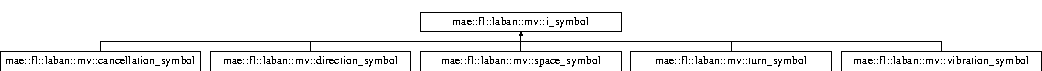
\includegraphics[height=0.953192cm]{classmae_1_1fl_1_1laban_1_1mv_1_1i__symbol}
\end{center}
\end{figure}
\subsection*{Public Member Functions}
\begin{DoxyCompactItemize}
\item 
virtual bool \hyperlink{classmae_1_1fl_1_1laban_1_1mv_1_1i__symbol_a78d90af5e1da4a6561d7545a76689d0e}{equals} (std\-::shared\-\_\-ptr$<$ \hyperlink{classmae_1_1fl_1_1laban_1_1mv_1_1i__symbol}{i\-\_\-symbol} $>$ a) const =0
\item 
virtual std\-::string \hyperlink{classmae_1_1fl_1_1laban_1_1mv_1_1i__symbol_a05d0b0c74bad854d5e9e3291bbd87b0d}{xml} (unsigned int indent=0, std\-::string namesp=\char`\"{}\char`\"{}) const =0
\item 
virtual std\-::string \hyperlink{classmae_1_1fl_1_1laban_1_1mv_1_1i__symbol_ae0a724c98c27c05fdde9afff99184029}{svg} (std\-::string identifier, double posx, double posy, double width, double height, bool left=false) const =0
\item 
virtual std\-::string \hyperlink{classmae_1_1fl_1_1laban_1_1mv_1_1i__symbol_ad254351eabf06ac945c168b24643872e}{str} () const =0
\end{DoxyCompactItemize}
\subsection*{Friends}
\begin{DoxyCompactItemize}
\item 
\hypertarget{classmae_1_1fl_1_1laban_1_1mv_1_1i__symbol_a0bf03a8d669d7f69cbe39b31d29113d4}{std\-::ostream \& {\bfseries operator$<$$<$} (std\-::ostream \&os, const \hyperlink{classmae_1_1fl_1_1laban_1_1mv_1_1i__symbol}{i\-\_\-symbol} \&obj)}\label{classmae_1_1fl_1_1laban_1_1mv_1_1i__symbol_a0bf03a8d669d7f69cbe39b31d29113d4}

\item 
\hypertarget{classmae_1_1fl_1_1laban_1_1mv_1_1i__symbol_aa68caef88df1b1bb458a0facaeacd050}{std\-::ostream \& {\bfseries operator$<$$<$} (std\-::ostream \&os, const std\-::shared\-\_\-ptr$<$ \hyperlink{classmae_1_1fl_1_1laban_1_1mv_1_1i__symbol}{i\-\_\-symbol} $>$ \&obj)}\label{classmae_1_1fl_1_1laban_1_1mv_1_1i__symbol_aa68caef88df1b1bb458a0facaeacd050}

\end{DoxyCompactItemize}


\subsection{Member Function Documentation}
\hypertarget{classmae_1_1fl_1_1laban_1_1mv_1_1i__symbol_a78d90af5e1da4a6561d7545a76689d0e}{\index{mae\-::fl\-::laban\-::mv\-::i\-\_\-symbol@{mae\-::fl\-::laban\-::mv\-::i\-\_\-symbol}!equals@{equals}}
\index{equals@{equals}!mae::fl::laban::mv::i_symbol@{mae\-::fl\-::laban\-::mv\-::i\-\_\-symbol}}
\subsubsection[{equals}]{\setlength{\rightskip}{0pt plus 5cm}virtual bool mae\-::fl\-::laban\-::mv\-::i\-\_\-symbol\-::equals (
\begin{DoxyParamCaption}
\item[{std\-::shared\-\_\-ptr$<$ {\bf i\-\_\-symbol} $>$}]{a}
\end{DoxyParamCaption}
) const\hspace{0.3cm}{\ttfamily [pure virtual]}}}\label{classmae_1_1fl_1_1laban_1_1mv_1_1i__symbol_a78d90af5e1da4a6561d7545a76689d0e}
Returns true if signs are equal.


\begin{DoxyParams}{Parameters}
{\em a} & The sign to be compared to. \\
\hline
\end{DoxyParams}
\begin{DoxyReturn}{Returns}
True if equal. 
\end{DoxyReturn}


Implemented in \hyperlink{classmae_1_1fl_1_1laban_1_1mv_1_1direction__symbol_a2ea85fd4be221d8dc2da7ee417dd829c}{mae\-::fl\-::laban\-::mv\-::direction\-\_\-symbol}, \hyperlink{classmae_1_1fl_1_1laban_1_1mv_1_1vibration__symbol_a65444ca2f4c0f7845ea3a48375379d65}{mae\-::fl\-::laban\-::mv\-::vibration\-\_\-symbol}, \hyperlink{classmae_1_1fl_1_1laban_1_1mv_1_1turn__symbol_aafc1b11568db52d9fa3fbc86a7c281c2}{mae\-::fl\-::laban\-::mv\-::turn\-\_\-symbol}, \hyperlink{classmae_1_1fl_1_1laban_1_1mv_1_1space__symbol_a9079a63e55fca3b2e8232fed1ef65e06}{mae\-::fl\-::laban\-::mv\-::space\-\_\-symbol}, and \hyperlink{classmae_1_1fl_1_1laban_1_1mv_1_1cancellation__symbol_a158d3eee246e2e8eda8a8884a209beca}{mae\-::fl\-::laban\-::mv\-::cancellation\-\_\-symbol}.

\hypertarget{classmae_1_1fl_1_1laban_1_1mv_1_1i__symbol_ad254351eabf06ac945c168b24643872e}{\index{mae\-::fl\-::laban\-::mv\-::i\-\_\-symbol@{mae\-::fl\-::laban\-::mv\-::i\-\_\-symbol}!str@{str}}
\index{str@{str}!mae::fl::laban::mv::i_symbol@{mae\-::fl\-::laban\-::mv\-::i\-\_\-symbol}}
\subsubsection[{str}]{\setlength{\rightskip}{0pt plus 5cm}virtual std\-::string mae\-::fl\-::laban\-::mv\-::i\-\_\-symbol\-::str (
\begin{DoxyParamCaption}
{}
\end{DoxyParamCaption}
) const\hspace{0.3cm}{\ttfamily [pure virtual]}}}\label{classmae_1_1fl_1_1laban_1_1mv_1_1i__symbol_ad254351eabf06ac945c168b24643872e}
Returns the string representation for this element.

\begin{DoxyReturn}{Returns}
The string. 
\end{DoxyReturn}


Implemented in \hyperlink{classmae_1_1fl_1_1laban_1_1mv_1_1direction__symbol_a3d6beaca72898fa289efd8dfc7e283f7}{mae\-::fl\-::laban\-::mv\-::direction\-\_\-symbol}, \hyperlink{classmae_1_1fl_1_1laban_1_1mv_1_1vibration__symbol_a6dfa83223bd1d96244268806f6d7f8b5}{mae\-::fl\-::laban\-::mv\-::vibration\-\_\-symbol}, \hyperlink{classmae_1_1fl_1_1laban_1_1mv_1_1turn__symbol_a92bc9681ef076940af9412fde943cf0c}{mae\-::fl\-::laban\-::mv\-::turn\-\_\-symbol}, \hyperlink{classmae_1_1fl_1_1laban_1_1mv_1_1space__symbol_ac528043832637bf9186a3dda3604c418}{mae\-::fl\-::laban\-::mv\-::space\-\_\-symbol}, and \hyperlink{classmae_1_1fl_1_1laban_1_1mv_1_1cancellation__symbol_aa2ff5bbb5398aa454e7995eeb8c1f31a}{mae\-::fl\-::laban\-::mv\-::cancellation\-\_\-symbol}.

\hypertarget{classmae_1_1fl_1_1laban_1_1mv_1_1i__symbol_ae0a724c98c27c05fdde9afff99184029}{\index{mae\-::fl\-::laban\-::mv\-::i\-\_\-symbol@{mae\-::fl\-::laban\-::mv\-::i\-\_\-symbol}!svg@{svg}}
\index{svg@{svg}!mae::fl::laban::mv::i_symbol@{mae\-::fl\-::laban\-::mv\-::i\-\_\-symbol}}
\subsubsection[{svg}]{\setlength{\rightskip}{0pt plus 5cm}virtual std\-::string mae\-::fl\-::laban\-::mv\-::i\-\_\-symbol\-::svg (
\begin{DoxyParamCaption}
\item[{std\-::string}]{identifier, }
\item[{double}]{posx, }
\item[{double}]{posy, }
\item[{double}]{width, }
\item[{double}]{height, }
\item[{bool}]{left = {\ttfamily false}}
\end{DoxyParamCaption}
) const\hspace{0.3cm}{\ttfamily [pure virtual]}}}\label{classmae_1_1fl_1_1laban_1_1mv_1_1i__symbol_ae0a724c98c27c05fdde9afff99184029}
Returns the S\-V\-G representation for this symbol.


\begin{DoxyParams}{Parameters}
{\em posx} & The x position. \\
\hline
{\em posy} & The y position. \\
\hline
{\em width} & The width. \\
\hline
{\em height} & The height. \\
\hline
\end{DoxyParams}
\begin{DoxyReturn}{Returns}
The S\-V\-G. 
\end{DoxyReturn}


Implemented in \hyperlink{classmae_1_1fl_1_1laban_1_1mv_1_1direction__symbol_af0e41f900f48beafee3e8daeade9687e}{mae\-::fl\-::laban\-::mv\-::direction\-\_\-symbol}, \hyperlink{classmae_1_1fl_1_1laban_1_1mv_1_1vibration__symbol_af8f13853392a942ceb8ceb00f3af5e47}{mae\-::fl\-::laban\-::mv\-::vibration\-\_\-symbol}, \hyperlink{classmae_1_1fl_1_1laban_1_1mv_1_1turn__symbol_a756844c1207460af1d2f08245f0128b9}{mae\-::fl\-::laban\-::mv\-::turn\-\_\-symbol}, \hyperlink{classmae_1_1fl_1_1laban_1_1mv_1_1space__symbol_ae6c9b408da1fcbc53881471035b496bd}{mae\-::fl\-::laban\-::mv\-::space\-\_\-symbol}, and \hyperlink{classmae_1_1fl_1_1laban_1_1mv_1_1cancellation__symbol_a63cb4ffd49386728f18001301a2b29e3}{mae\-::fl\-::laban\-::mv\-::cancellation\-\_\-symbol}.

\hypertarget{classmae_1_1fl_1_1laban_1_1mv_1_1i__symbol_a05d0b0c74bad854d5e9e3291bbd87b0d}{\index{mae\-::fl\-::laban\-::mv\-::i\-\_\-symbol@{mae\-::fl\-::laban\-::mv\-::i\-\_\-symbol}!xml@{xml}}
\index{xml@{xml}!mae::fl::laban::mv::i_symbol@{mae\-::fl\-::laban\-::mv\-::i\-\_\-symbol}}
\subsubsection[{xml}]{\setlength{\rightskip}{0pt plus 5cm}virtual std\-::string mae\-::fl\-::laban\-::mv\-::i\-\_\-symbol\-::xml (
\begin{DoxyParamCaption}
\item[{unsigned int}]{indent = {\ttfamily 0}, }
\item[{std\-::string}]{namesp = {\ttfamily \char`\"{}\char`\"{}}}
\end{DoxyParamCaption}
) const\hspace{0.3cm}{\ttfamily [pure virtual]}}}\label{classmae_1_1fl_1_1laban_1_1mv_1_1i__symbol_a05d0b0c74bad854d5e9e3291bbd87b0d}
Returns the X\-M\-L representation for this element.


\begin{DoxyParams}{Parameters}
{\em indent} & The applied indent. \\
\hline
{\em namesp} & The prefixed X\-M\-L namespace.\\
\hline
\end{DoxyParams}
\begin{DoxyReturn}{Returns}
The X\-M\-L string. 
\end{DoxyReturn}


Implemented in \hyperlink{classmae_1_1fl_1_1laban_1_1mv_1_1direction__symbol_a987e147f6a6ae37e50d450f382d850c1}{mae\-::fl\-::laban\-::mv\-::direction\-\_\-symbol}, \hyperlink{classmae_1_1fl_1_1laban_1_1mv_1_1vibration__symbol_adaec2bb356fd6321c9585651301e1ac7}{mae\-::fl\-::laban\-::mv\-::vibration\-\_\-symbol}, \hyperlink{classmae_1_1fl_1_1laban_1_1mv_1_1turn__symbol_a4b404fcb4b74a4db80b47cabb7876afa}{mae\-::fl\-::laban\-::mv\-::turn\-\_\-symbol}, \hyperlink{classmae_1_1fl_1_1laban_1_1mv_1_1space__symbol_a5aa4290ae8e7473dc5d0ef435f3035b7}{mae\-::fl\-::laban\-::mv\-::space\-\_\-symbol}, and \hyperlink{classmae_1_1fl_1_1laban_1_1mv_1_1cancellation__symbol_a17122710f983a1b7308c7103e5e9e222}{mae\-::fl\-::laban\-::mv\-::cancellation\-\_\-symbol}.



The documentation for this class was generated from the following file\-:\begin{DoxyCompactItemize}
\item 
src/mae/fl/laban/mv/i\-\_\-symbol.\-hpp\end{DoxyCompactItemize}

\hypertarget{classmae_1_1ini__reader}{\section{mae\-:\-:ini\-\_\-reader Class Reference}
\label{classmae_1_1ini__reader}\index{mae\-::ini\-\_\-reader@{mae\-::ini\-\_\-reader}}
}
\subsection*{Public Member Functions}
\begin{DoxyCompactItemize}
\item 
\hyperlink{classmae_1_1ini__reader_a796f4ee57ccf99f2e111e11cb30d8c5d}{ini\-\_\-reader} (std\-::string file)
\item 
virtual std\-::string \hyperlink{classmae_1_1ini__reader_a422cd348ae6645d3860c26c3b80e765f}{get\-\_\-value} (std\-::string domain, std\-::string key)
\item 
virtual bool \hyperlink{classmae_1_1ini__reader_a568ce2cafc35b019a908b60444931f56}{get\-\_\-value\-\_\-nex} (std\-::string domain, std\-::string key, std\-::string $\ast$result)
\item 
virtual bool \hyperlink{classmae_1_1ini__reader_a9991b7c00c092ded8182170342849ac7}{get\-\_\-value\-\_\-nex} (std\-::string domain, std\-::string key, std\-::string $\ast$result, std\-::string $\ast$out\-\_\-error\-\_\-msg)
\end{DoxyCompactItemize}


\subsection{Constructor \& Destructor Documentation}
\hypertarget{classmae_1_1ini__reader_a796f4ee57ccf99f2e111e11cb30d8c5d}{\index{mae\-::ini\-\_\-reader@{mae\-::ini\-\_\-reader}!ini\-\_\-reader@{ini\-\_\-reader}}
\index{ini\-\_\-reader@{ini\-\_\-reader}!mae::ini_reader@{mae\-::ini\-\_\-reader}}
\subsubsection[{ini\-\_\-reader}]{\setlength{\rightskip}{0pt plus 5cm}mae\-::ini\-\_\-reader\-::ini\-\_\-reader (
\begin{DoxyParamCaption}
\item[{std\-::string}]{file}
\end{DoxyParamCaption}
)}}\label{classmae_1_1ini__reader_a796f4ee57ccf99f2e111e11cb30d8c5d}
Creates a new ini reader. Reads the file and allows access via this class.


\begin{DoxyParams}{Parameters}
{\em file} & \\
\hline
\end{DoxyParams}


\subsection{Member Function Documentation}
\hypertarget{classmae_1_1ini__reader_a422cd348ae6645d3860c26c3b80e765f}{\index{mae\-::ini\-\_\-reader@{mae\-::ini\-\_\-reader}!get\-\_\-value@{get\-\_\-value}}
\index{get\-\_\-value@{get\-\_\-value}!mae::ini_reader@{mae\-::ini\-\_\-reader}}
\subsubsection[{get\-\_\-value}]{\setlength{\rightskip}{0pt plus 5cm}std\-::string mae\-::ini\-\_\-reader\-::get\-\_\-value (
\begin{DoxyParamCaption}
\item[{std\-::string}]{domain, }
\item[{std\-::string}]{key}
\end{DoxyParamCaption}
)\hspace{0.3cm}{\ttfamily [virtual]}}}\label{classmae_1_1ini__reader_a422cd348ae6645d3860c26c3b80e765f}
Returns the value assigned to the key in the given domain.


\begin{DoxyParams}{Parameters}
{\em domain} & The domain. \char`\"{}\char`\"{} if no domain \\
\hline
{\em key} & The key for the element. \\
\hline
\end{DoxyParams}
\begin{DoxyReturn}{Returns}
The value. 
\end{DoxyReturn}
\hypertarget{classmae_1_1ini__reader_a568ce2cafc35b019a908b60444931f56}{\index{mae\-::ini\-\_\-reader@{mae\-::ini\-\_\-reader}!get\-\_\-value\-\_\-nex@{get\-\_\-value\-\_\-nex}}
\index{get\-\_\-value\-\_\-nex@{get\-\_\-value\-\_\-nex}!mae::ini_reader@{mae\-::ini\-\_\-reader}}
\subsubsection[{get\-\_\-value\-\_\-nex}]{\setlength{\rightskip}{0pt plus 5cm}bool mae\-::ini\-\_\-reader\-::get\-\_\-value\-\_\-nex (
\begin{DoxyParamCaption}
\item[{std\-::string}]{domain, }
\item[{std\-::string}]{key, }
\item[{std\-::string $\ast$}]{result}
\end{DoxyParamCaption}
)\hspace{0.3cm}{\ttfamily [virtual]}}}\label{classmae_1_1ini__reader_a568ce2cafc35b019a908b60444931f56}
Returns the value assigned to the key in the given domain. Suppresses the exception.


\begin{DoxyParams}{Parameters}
{\em domain} & The domain. \char`\"{}\char`\"{} if no domain \\
\hline
{\em key} & The key for the element. \\
\hline
\end{DoxyParams}
\begin{DoxyReturn}{Returns}
The value. 
\end{DoxyReturn}

\begin{DoxyParams}{Parameters}
{\em result} & The pointer where to write the result. \\
\hline
\end{DoxyParams}
\begin{DoxyReturn}{Returns}
True if successful. 
\end{DoxyReturn}
\hypertarget{classmae_1_1ini__reader_a9991b7c00c092ded8182170342849ac7}{\index{mae\-::ini\-\_\-reader@{mae\-::ini\-\_\-reader}!get\-\_\-value\-\_\-nex@{get\-\_\-value\-\_\-nex}}
\index{get\-\_\-value\-\_\-nex@{get\-\_\-value\-\_\-nex}!mae::ini_reader@{mae\-::ini\-\_\-reader}}
\subsubsection[{get\-\_\-value\-\_\-nex}]{\setlength{\rightskip}{0pt plus 5cm}bool mae\-::ini\-\_\-reader\-::get\-\_\-value\-\_\-nex (
\begin{DoxyParamCaption}
\item[{std\-::string}]{domain, }
\item[{std\-::string}]{key, }
\item[{std\-::string $\ast$}]{result, }
\item[{std\-::string $\ast$}]{out\-\_\-error\-\_\-msg}
\end{DoxyParamCaption}
)\hspace{0.3cm}{\ttfamily [virtual]}}}\label{classmae_1_1ini__reader_a9991b7c00c092ded8182170342849ac7}
Returns the value assigned to the key in the given domain. Suppresses the exception.


\begin{DoxyParams}{Parameters}
{\em domain} & The domain. \char`\"{}\char`\"{} if no domain \\
\hline
{\em key} & The key for the element. \\
\hline
\end{DoxyParams}
\begin{DoxyReturn}{Returns}
The value. 
\end{DoxyReturn}

\begin{DoxyParams}{Parameters}
{\em result} & The pointer where to write the result. \\
\hline
{\em out\-\_\-error\-\_\-msg} & The pointer where to write the error message. \\
\hline
\end{DoxyParams}
\begin{DoxyReturn}{Returns}
True if successful. 
\end{DoxyReturn}


The documentation for this class was generated from the following files\-:\begin{DoxyCompactItemize}
\item 
src/mae/ini\-\_\-reader.\-hpp\item 
src/mae/ini\-\_\-reader.\-cpp\end{DoxyCompactItemize}

\hypertarget{classmae_1_1fl_1_1laban_1_1ps_1_1joint__part}{\section{mae\-:\-:fl\-:\-:laban\-:\-:ps\-:\-:joint\-\_\-part Class Reference}
\label{classmae_1_1fl_1_1laban_1_1ps_1_1joint__part}\index{mae\-::fl\-::laban\-::ps\-::joint\-\_\-part@{mae\-::fl\-::laban\-::ps\-::joint\-\_\-part}}
}
Inheritance diagram for mae\-:\-:fl\-:\-:laban\-:\-:ps\-:\-:joint\-\_\-part\-:\begin{figure}[H]
\begin{center}
\leavevmode
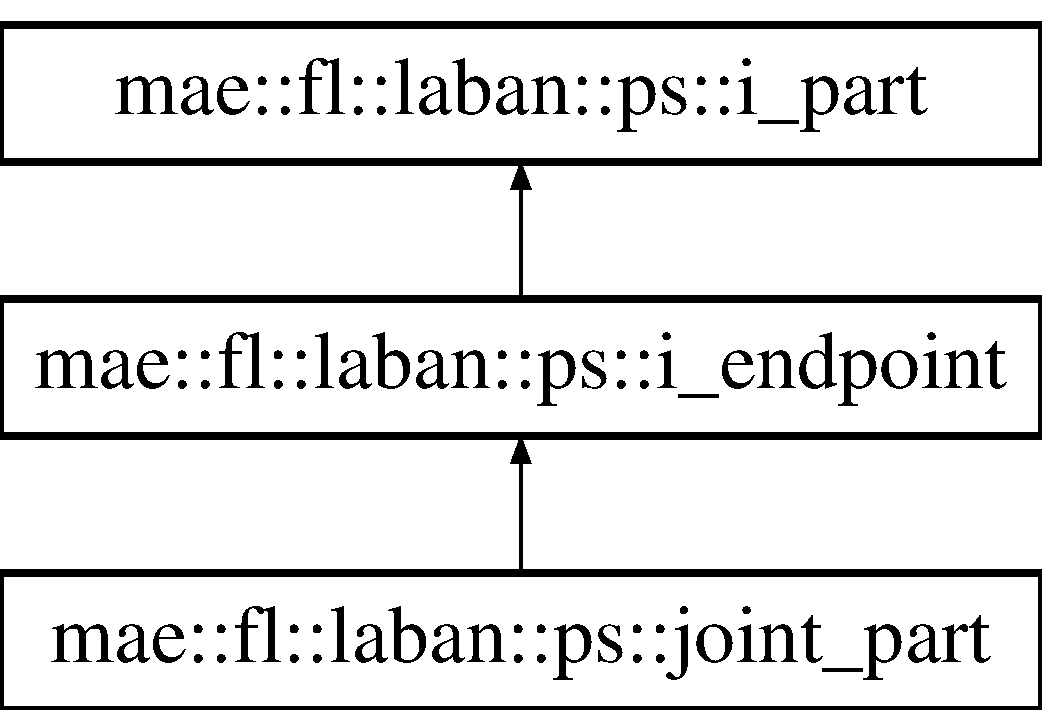
\includegraphics[height=3.000000cm]{classmae_1_1fl_1_1laban_1_1ps_1_1joint__part}
\end{center}
\end{figure}
\subsection*{Public Member Functions}
\begin{DoxyCompactItemize}
\item 
\hyperlink{classmae_1_1fl_1_1laban_1_1ps_1_1joint__part_a7f762c967cd8f22d1f82f5cf15c3de5f}{joint\-\_\-part} (e\-\_\-joint joint)
\item 
e\-\_\-joint \hyperlink{classmae_1_1fl_1_1laban_1_1ps_1_1joint__part_aa7ac33b4e1af216f9359f3f0cb493c0b}{get\-\_\-joint} () const 
\item 
virtual std\-::string \hyperlink{classmae_1_1fl_1_1laban_1_1ps_1_1joint__part_a3054936a94c43d4cb3cb21745234e2cf}{xml} (unsigned int indent=0, std\-::string namesp=\char`\"{}\char`\"{}) const 
\item 
virtual std\-::string \hyperlink{classmae_1_1fl_1_1laban_1_1ps_1_1joint__part_af8e8475612c99842a6b6a18964168592}{svg} (std\-::string identifier, double posx, double posy, double width, double height, bool left=false) const 
\item 
virtual std\-::shared\-\_\-ptr\\*
$<$ \hyperlink{classmae_1_1fl_1_1laban_1_1ps_1_1i__endpoint}{i\-\_\-endpoint} $>$ \hyperlink{classmae_1_1fl_1_1laban_1_1ps_1_1joint__part_a08d427668f18131036b88c2156ccdd3f}{get\-\_\-fixed\-\_\-end} () const 
\item 
virtual bool \hyperlink{classmae_1_1fl_1_1laban_1_1ps_1_1joint__part_a1de75536e4a12e1435e0ec3c4f2edbad}{equals} (std\-::shared\-\_\-ptr$<$ \hyperlink{classmae_1_1fl_1_1laban_1_1ps_1_1i__part}{i\-\_\-part} $>$ a) const 
\item 
virtual bool \hyperlink{classmae_1_1fl_1_1laban_1_1ps_1_1joint__part_ad159de6d5a1adb07b76a4a151541569e}{equals} (std\-::shared\-\_\-ptr$<$ \hyperlink{classmae_1_1fl_1_1laban_1_1ps_1_1i__endpoint}{i\-\_\-endpoint} $>$ a) const 
\end{DoxyCompactItemize}


\subsection{Constructor \& Destructor Documentation}
\hypertarget{classmae_1_1fl_1_1laban_1_1ps_1_1joint__part_a7f762c967cd8f22d1f82f5cf15c3de5f}{\index{mae\-::fl\-::laban\-::ps\-::joint\-\_\-part@{mae\-::fl\-::laban\-::ps\-::joint\-\_\-part}!joint\-\_\-part@{joint\-\_\-part}}
\index{joint\-\_\-part@{joint\-\_\-part}!mae::fl::laban::ps::joint_part@{mae\-::fl\-::laban\-::ps\-::joint\-\_\-part}}
\subsubsection[{joint\-\_\-part}]{\setlength{\rightskip}{0pt plus 5cm}mae\-::fl\-::laban\-::ps\-::joint\-\_\-part\-::joint\-\_\-part (
\begin{DoxyParamCaption}
\item[{e\-\_\-joint}]{joint}
\end{DoxyParamCaption}
)}}\label{classmae_1_1fl_1_1laban_1_1ps_1_1joint__part_a7f762c967cd8f22d1f82f5cf15c3de5f}
Creates a joint part used for a pre-\/sign.


\begin{DoxyParams}{Parameters}
{\em joint} & The addressed joint. \\
\hline
\end{DoxyParams}


\subsection{Member Function Documentation}
\hypertarget{classmae_1_1fl_1_1laban_1_1ps_1_1joint__part_a1de75536e4a12e1435e0ec3c4f2edbad}{\index{mae\-::fl\-::laban\-::ps\-::joint\-\_\-part@{mae\-::fl\-::laban\-::ps\-::joint\-\_\-part}!equals@{equals}}
\index{equals@{equals}!mae::fl::laban::ps::joint_part@{mae\-::fl\-::laban\-::ps\-::joint\-\_\-part}}
\subsubsection[{equals}]{\setlength{\rightskip}{0pt plus 5cm}bool mae\-::fl\-::laban\-::ps\-::joint\-\_\-part\-::equals (
\begin{DoxyParamCaption}
\item[{std\-::shared\-\_\-ptr$<$ {\bf i\-\_\-part} $>$}]{a}
\end{DoxyParamCaption}
) const\hspace{0.3cm}{\ttfamily [virtual]}}}\label{classmae_1_1fl_1_1laban_1_1ps_1_1joint__part_a1de75536e4a12e1435e0ec3c4f2edbad}
Returns true if elements are equal.


\begin{DoxyParams}{Parameters}
{\em a} & The element to be compared to. \\
\hline
\end{DoxyParams}
\begin{DoxyReturn}{Returns}
True if equal. 
\end{DoxyReturn}


Implements \hyperlink{classmae_1_1fl_1_1laban_1_1ps_1_1i__endpoint_abc675b07d3ce69fbec362b2e792a1e06}{mae\-::fl\-::laban\-::ps\-::i\-\_\-endpoint}.

\hypertarget{classmae_1_1fl_1_1laban_1_1ps_1_1joint__part_ad159de6d5a1adb07b76a4a151541569e}{\index{mae\-::fl\-::laban\-::ps\-::joint\-\_\-part@{mae\-::fl\-::laban\-::ps\-::joint\-\_\-part}!equals@{equals}}
\index{equals@{equals}!mae::fl::laban::ps::joint_part@{mae\-::fl\-::laban\-::ps\-::joint\-\_\-part}}
\subsubsection[{equals}]{\setlength{\rightskip}{0pt plus 5cm}bool mae\-::fl\-::laban\-::ps\-::joint\-\_\-part\-::equals (
\begin{DoxyParamCaption}
\item[{std\-::shared\-\_\-ptr$<$ {\bf i\-\_\-endpoint} $>$}]{a}
\end{DoxyParamCaption}
) const\hspace{0.3cm}{\ttfamily [virtual]}}}\label{classmae_1_1fl_1_1laban_1_1ps_1_1joint__part_ad159de6d5a1adb07b76a4a151541569e}
Returns true if elements are equal.


\begin{DoxyParams}{Parameters}
{\em a} & The element to be compared to. \\
\hline
\end{DoxyParams}
\begin{DoxyReturn}{Returns}
True if equal. 
\end{DoxyReturn}


Implements \hyperlink{classmae_1_1fl_1_1laban_1_1ps_1_1i__endpoint_aeffb14c43728d2ef094122f3d0278455}{mae\-::fl\-::laban\-::ps\-::i\-\_\-endpoint}.

\hypertarget{classmae_1_1fl_1_1laban_1_1ps_1_1joint__part_a08d427668f18131036b88c2156ccdd3f}{\index{mae\-::fl\-::laban\-::ps\-::joint\-\_\-part@{mae\-::fl\-::laban\-::ps\-::joint\-\_\-part}!get\-\_\-fixed\-\_\-end@{get\-\_\-fixed\-\_\-end}}
\index{get\-\_\-fixed\-\_\-end@{get\-\_\-fixed\-\_\-end}!mae::fl::laban::ps::joint_part@{mae\-::fl\-::laban\-::ps\-::joint\-\_\-part}}
\subsubsection[{get\-\_\-fixed\-\_\-end}]{\setlength{\rightskip}{0pt plus 5cm}std\-::shared\-\_\-ptr$<$ {\bf i\-\_\-endpoint} $>$ mae\-::fl\-::laban\-::ps\-::joint\-\_\-part\-::get\-\_\-fixed\-\_\-end (
\begin{DoxyParamCaption}
{}
\end{DoxyParamCaption}
) const\hspace{0.3cm}{\ttfamily [virtual]}}}\label{classmae_1_1fl_1_1laban_1_1ps_1_1joint__part_a08d427668f18131036b88c2156ccdd3f}
Returns the predecessor of the current endpoint (which is the default fixed endpoint). If the endpoint is the beginning of the extremity null is returned.

\begin{DoxyReturn}{Returns}
The successor element. 
\end{DoxyReturn}


Implements \hyperlink{classmae_1_1fl_1_1laban_1_1ps_1_1i__endpoint_a0938824cc5892b072636c3b52352b3f2}{mae\-::fl\-::laban\-::ps\-::i\-\_\-endpoint}.

\hypertarget{classmae_1_1fl_1_1laban_1_1ps_1_1joint__part_aa7ac33b4e1af216f9359f3f0cb493c0b}{\index{mae\-::fl\-::laban\-::ps\-::joint\-\_\-part@{mae\-::fl\-::laban\-::ps\-::joint\-\_\-part}!get\-\_\-joint@{get\-\_\-joint}}
\index{get\-\_\-joint@{get\-\_\-joint}!mae::fl::laban::ps::joint_part@{mae\-::fl\-::laban\-::ps\-::joint\-\_\-part}}
\subsubsection[{get\-\_\-joint}]{\setlength{\rightskip}{0pt plus 5cm}e\-\_\-joint mae\-::fl\-::laban\-::ps\-::joint\-\_\-part\-::get\-\_\-joint (
\begin{DoxyParamCaption}
{}
\end{DoxyParamCaption}
) const}}\label{classmae_1_1fl_1_1laban_1_1ps_1_1joint__part_aa7ac33b4e1af216f9359f3f0cb493c0b}
Returns the addressed joint. \begin{DoxyReturn}{Returns}

\end{DoxyReturn}
\hypertarget{classmae_1_1fl_1_1laban_1_1ps_1_1joint__part_af8e8475612c99842a6b6a18964168592}{\index{mae\-::fl\-::laban\-::ps\-::joint\-\_\-part@{mae\-::fl\-::laban\-::ps\-::joint\-\_\-part}!svg@{svg}}
\index{svg@{svg}!mae::fl::laban::ps::joint_part@{mae\-::fl\-::laban\-::ps\-::joint\-\_\-part}}
\subsubsection[{svg}]{\setlength{\rightskip}{0pt plus 5cm}std\-::string mae\-::fl\-::laban\-::ps\-::joint\-\_\-part\-::svg (
\begin{DoxyParamCaption}
\item[{std\-::string}]{identifier, }
\item[{double}]{posx, }
\item[{double}]{posy, }
\item[{double}]{width, }
\item[{double}]{height, }
\item[{bool}]{left = {\ttfamily false}}
\end{DoxyParamCaption}
) const\hspace{0.3cm}{\ttfamily [virtual]}}}\label{classmae_1_1fl_1_1laban_1_1ps_1_1joint__part_af8e8475612c99842a6b6a18964168592}
Returns the S\-V\-G representation for this symbol.


\begin{DoxyParams}{Parameters}
{\em posx} & The x position. \\
\hline
{\em posy} & The y position. \\
\hline
{\em width} & The width. \\
\hline
{\em height} & The height. \\
\hline
\end{DoxyParams}
\begin{DoxyReturn}{Returns}
The S\-V\-G. 
\end{DoxyReturn}


Implements \hyperlink{classmae_1_1fl_1_1laban_1_1ps_1_1i__part_a78227d5ecd87655a7a9454c68f470368}{mae\-::fl\-::laban\-::ps\-::i\-\_\-part}.

\hypertarget{classmae_1_1fl_1_1laban_1_1ps_1_1joint__part_a3054936a94c43d4cb3cb21745234e2cf}{\index{mae\-::fl\-::laban\-::ps\-::joint\-\_\-part@{mae\-::fl\-::laban\-::ps\-::joint\-\_\-part}!xml@{xml}}
\index{xml@{xml}!mae::fl::laban::ps::joint_part@{mae\-::fl\-::laban\-::ps\-::joint\-\_\-part}}
\subsubsection[{xml}]{\setlength{\rightskip}{0pt plus 5cm}std\-::string mae\-::fl\-::laban\-::ps\-::joint\-\_\-part\-::xml (
\begin{DoxyParamCaption}
\item[{unsigned int}]{indent = {\ttfamily 0}, }
\item[{std\-::string}]{namesp = {\ttfamily \char`\"{}\char`\"{}}}
\end{DoxyParamCaption}
) const\hspace{0.3cm}{\ttfamily [virtual]}}}\label{classmae_1_1fl_1_1laban_1_1ps_1_1joint__part_a3054936a94c43d4cb3cb21745234e2cf}
Returns the X\-M\-L representation for this element.


\begin{DoxyParams}{Parameters}
{\em indent} & The applied indent. \\
\hline
{\em namesp} & The prefixed X\-M\-L namespace.\\
\hline
\end{DoxyParams}
\begin{DoxyReturn}{Returns}
The X\-M\-L string. 
\end{DoxyReturn}


Implements \hyperlink{classmae_1_1fl_1_1laban_1_1ps_1_1i__endpoint_a1af7dbd05400cbdd7f9f45ef75dd38d6}{mae\-::fl\-::laban\-::ps\-::i\-\_\-endpoint}.



The documentation for this class was generated from the following files\-:\begin{DoxyCompactItemize}
\item 
src/mae/fl/laban/ps/joint\-\_\-part.\-hpp\item 
src/mae/fl/laban/ps/joint\-\_\-part.\-cpp\end{DoxyCompactItemize}

\hypertarget{classmae_1_1kp__detector}{\section{mae\-:\-:kp\-\_\-detector Class Reference}
\label{classmae_1_1kp__detector}\index{mae\-::kp\-\_\-detector@{mae\-::kp\-\_\-detector}}
}
Inheritance diagram for mae\-:\-:kp\-\_\-detector\-:\begin{figure}[H]
\begin{center}
\leavevmode
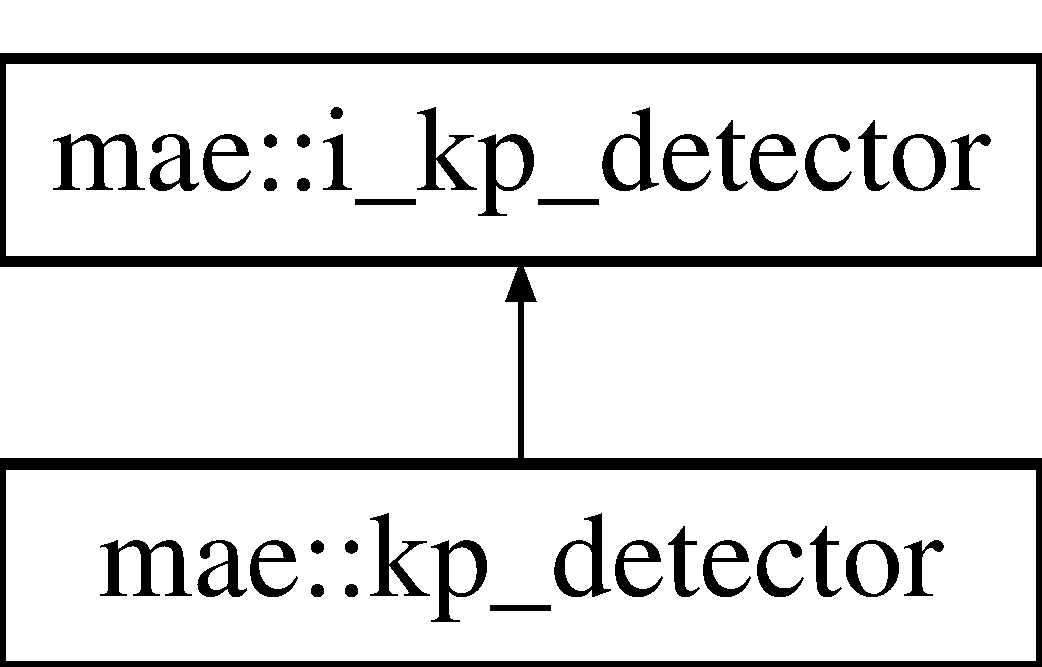
\includegraphics[height=2.000000cm]{classmae_1_1kp__detector}
\end{center}
\end{figure}
\subsection*{Public Member Functions}
\begin{DoxyCompactItemize}
\item 
\hyperlink{classmae_1_1kp__detector_acbf415da200c0e7345ea673898aa5d3f}{kp\-\_\-detector} (bool debug=false)
\item 
virtual std\-::shared\-\_\-ptr\\*
$<$ \hyperlink{classmae_1_1general__enriched__pose}{general\-\_\-enriched\-\_\-pose} $>$ \hyperlink{classmae_1_1kp__detector_a7aa02dc662f0a0abbefb0051fa783787}{estimate\-\_\-frame} (std\-::shared\-\_\-ptr$<$ \hyperlink{classmae_1_1general__pose}{general\-\_\-pose} $>$ current\-\_\-pose, std\-::list$<$ std\-::shared\-\_\-ptr$<$ \hyperlink{classmae_1_1general__enriched__pose}{general\-\_\-enriched\-\_\-pose} $>$ $>$ previous\-\_\-sequence, std\-::vector$<$ \hyperlink{classmae_1_1bone}{bone} $>$ body\-\_\-parts)
\end{DoxyCompactItemize}


\subsection{Constructor \& Destructor Documentation}
\hypertarget{classmae_1_1kp__detector_acbf415da200c0e7345ea673898aa5d3f}{\index{mae\-::kp\-\_\-detector@{mae\-::kp\-\_\-detector}!kp\-\_\-detector@{kp\-\_\-detector}}
\index{kp\-\_\-detector@{kp\-\_\-detector}!mae::kp_detector@{mae\-::kp\-\_\-detector}}
\subsubsection[{kp\-\_\-detector}]{\setlength{\rightskip}{0pt plus 5cm}mae\-::kp\-\_\-detector\-::kp\-\_\-detector (
\begin{DoxyParamCaption}
\item[{bool}]{debug = {\ttfamily false}}
\end{DoxyParamCaption}
)}}\label{classmae_1_1kp__detector_acbf415da200c0e7345ea673898aa5d3f}
Creates a new key pose detector.


\begin{DoxyParams}{Parameters}
{\em debug} & True if debug output shall be printed to the terminal. \\
\hline
\end{DoxyParams}


\subsection{Member Function Documentation}
\hypertarget{classmae_1_1kp__detector_a7aa02dc662f0a0abbefb0051fa783787}{\index{mae\-::kp\-\_\-detector@{mae\-::kp\-\_\-detector}!estimate\-\_\-frame@{estimate\-\_\-frame}}
\index{estimate\-\_\-frame@{estimate\-\_\-frame}!mae::kp_detector@{mae\-::kp\-\_\-detector}}
\subsubsection[{estimate\-\_\-frame}]{\setlength{\rightskip}{0pt plus 5cm}std\-::shared\-\_\-ptr$<$ {\bf general\-\_\-enriched\-\_\-pose} $>$ mae\-::kp\-\_\-detector\-::estimate\-\_\-frame (
\begin{DoxyParamCaption}
\item[{std\-::shared\-\_\-ptr$<$ {\bf general\-\_\-pose} $>$}]{current\-\_\-pose, }
\item[{std\-::list$<$ std\-::shared\-\_\-ptr$<$ {\bf general\-\_\-enriched\-\_\-pose} $>$ $>$}]{previous\-\_\-sequence, }
\item[{std\-::vector$<$ {\bf bone} $>$}]{body\-\_\-parts}
\end{DoxyParamCaption}
)\hspace{0.3cm}{\ttfamily [virtual]}}}\label{classmae_1_1kp__detector_a7aa02dc662f0a0abbefb0051fa783787}
Estimates the current frame and returns an enriched pose. Edits the given enriched poses, (e.\-g., sets key pose to false) but does not append the new enriched pose to the vector. Instead the new enriched pose is returned.


\begin{DoxyParams}{Parameters}
{\em current\-Pose} & The currently processed pose. \\
\hline
{\em previous\-Sequence} & The previous sequence which will be edited too. \\
\hline
{\em body\-Parts} & All body parts that shall be processed. \\
\hline
\end{DoxyParams}
\begin{DoxyReturn}{Returns}
The enriched pose. 
\end{DoxyReturn}


Implements \hyperlink{classmae_1_1i__kp__detector_a023a2719cd16be679c1101a9c27d21ac}{mae\-::i\-\_\-kp\-\_\-detector}.



The documentation for this class was generated from the following files\-:\begin{DoxyCompactItemize}
\item 
src/mae/kp\-\_\-detector.\-hpp\item 
src/mae/kp\-\_\-detector.\-cpp\end{DoxyCompactItemize}

\hypertarget{classmae_1_1kp__movement__detector}{\section{mae\-:\-:kp\-\_\-movement\-\_\-detector$<$ T, U $>$ Class Template Reference}
\label{classmae_1_1kp__movement__detector}\index{mae\-::kp\-\_\-movement\-\_\-detector$<$ T, U $>$@{mae\-::kp\-\_\-movement\-\_\-detector$<$ T, U $>$}}
}
Inheritance diagram for mae\-:\-:kp\-\_\-movement\-\_\-detector$<$ T, U $>$\-:\begin{figure}[H]
\begin{center}
\leavevmode
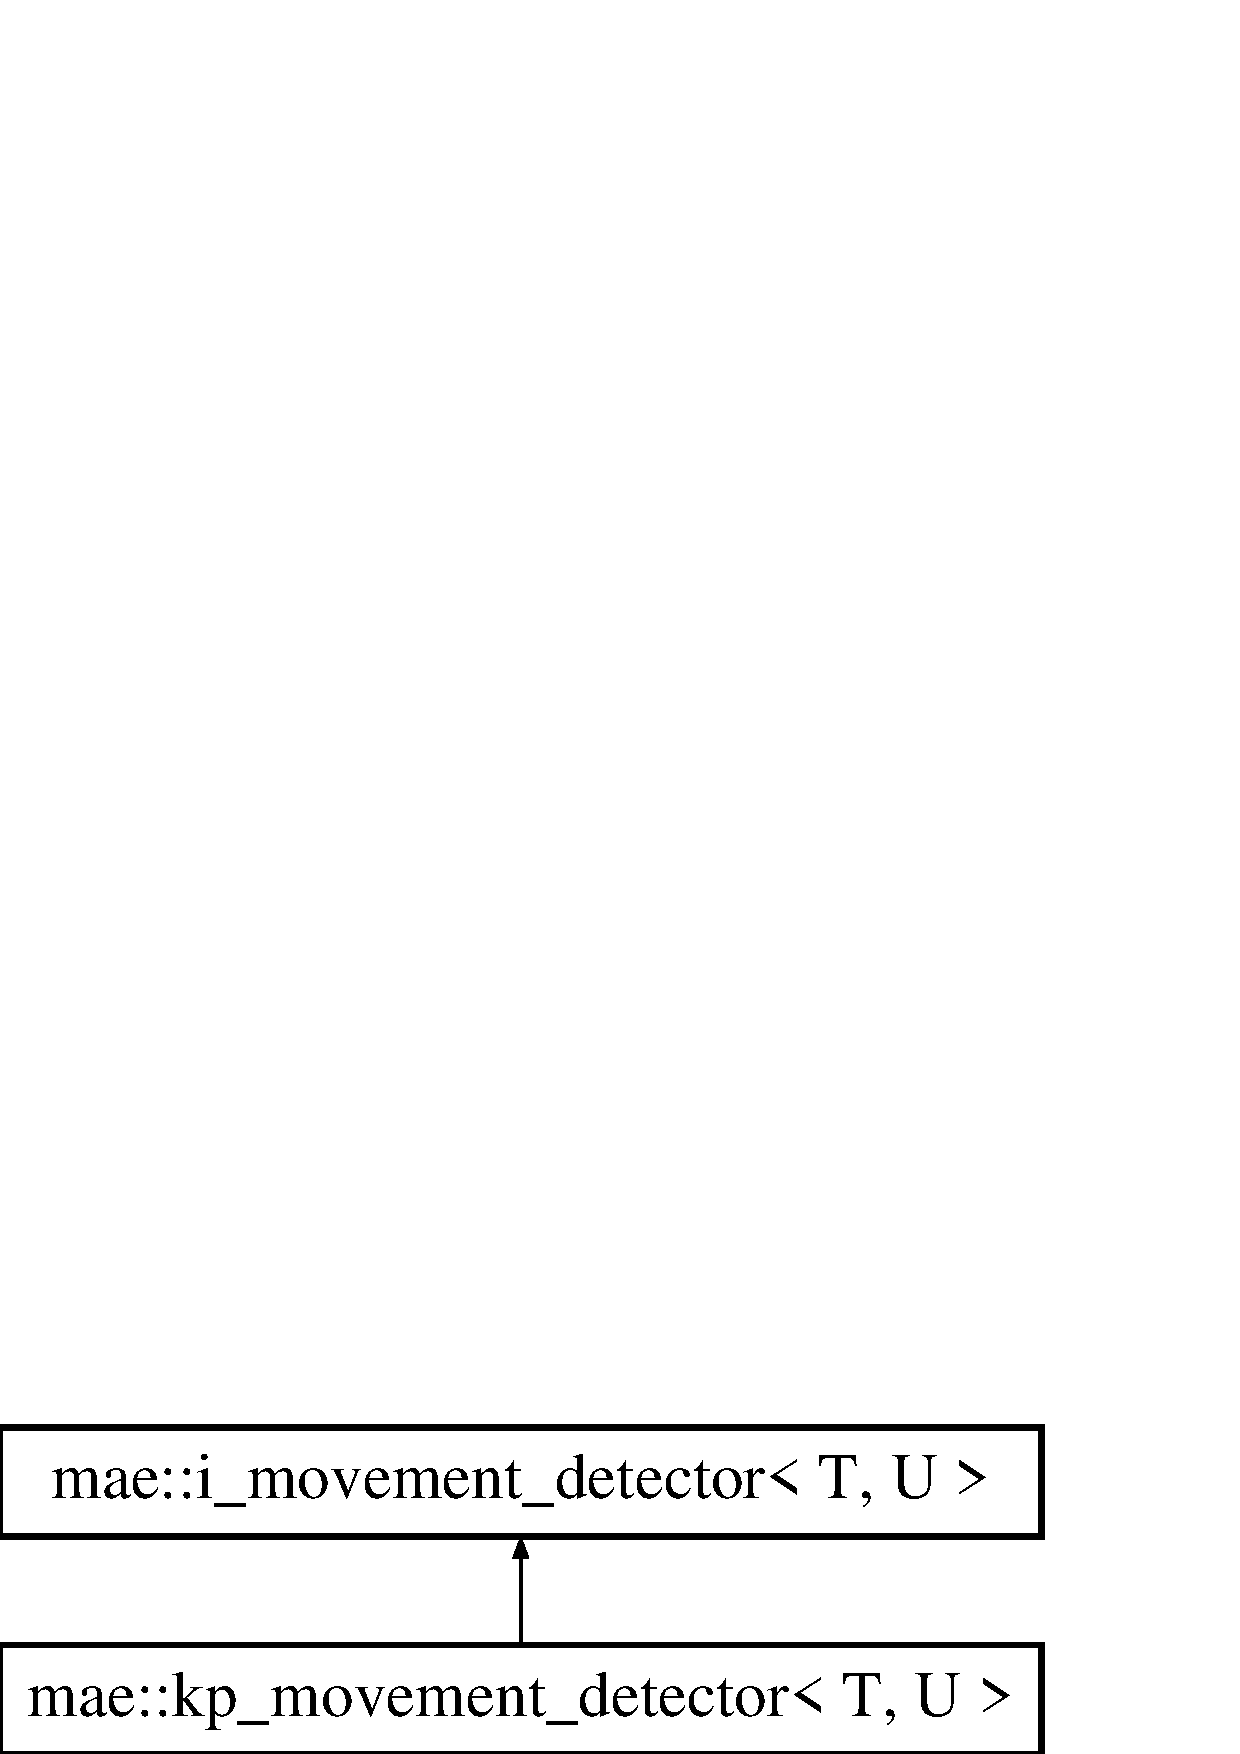
\includegraphics[height=2.000000cm]{classmae_1_1kp__movement__detector}
\end{center}
\end{figure}
\subsection*{Public Member Functions}
\begin{DoxyCompactItemize}
\item 
\hyperlink{classmae_1_1kp__movement__detector_a895e056f1ce3653b3ed71aec98b17941}{kp\-\_\-movement\-\_\-detector} (std\-::shared\-\_\-ptr$<$ \hyperlink{classmae_1_1i__pose__detector}{i\-\_\-pose\-\_\-detector}$<$ T $>$ $>$ ipd, std\-::shared\-\_\-ptr$<$ \hyperlink{classmae_1_1i__sequence__generator}{i\-\_\-sequence\-\_\-generator}$<$ U $>$ $>$ isg, bool debug=false)
\item 
\hyperlink{classmae_1_1kp__movement__detector_af9f13d86055607188453c57721d6227a}{kp\-\_\-movement\-\_\-detector} (std\-::shared\-\_\-ptr$<$ \hyperlink{classmae_1_1i__pose__detector}{i\-\_\-pose\-\_\-detector}$<$ T $>$ $>$ ipd, std\-::shared\-\_\-ptr$<$ \hyperlink{classmae_1_1i__sequence__generator}{i\-\_\-sequence\-\_\-generator}$<$ U $>$ $>$ isg, std\-::shared\-\_\-ptr$<$ \hyperlink{classmae_1_1i__kp__detector}{i\-\_\-kp\-\_\-detector} $>$ ikpd, bool debug=false)
\item 
virtual std\-::shared\-\_\-ptr$<$ U $>$ \hyperlink{classmae_1_1kp__movement__detector_a2aaa4c65a7735ac1d3ee201beb56b6b1}{detect\-\_\-movement} (long timestamp, double framerate, std\-::shared\-\_\-ptr$<$ T $>$ skeleton, std\-::vector$<$ \hyperlink{classmae_1_1bone}{bone} $>$ body\-\_\-parts)
\item 
virtual void \hyperlink{classmae_1_1kp__movement__detector_a673ed3ff4f7a5cd8a02cdbe254a4508e}{set\-\_\-buffer} (int size)
\item 
virtual void \hyperlink{classmae_1_1kp__movement__detector_a8fec5ae9e1f209fdcbeba3f86b5c3059}{clear\-\_\-buffer} ()
\item 
virtual void \hyperlink{classmae_1_1kp__movement__detector_a53f506b2d9c5bb759908a125af33f97d}{add\-\_\-listener} (std\-::shared\-\_\-ptr$<$ \hyperlink{classmae_1_1i__pose__listener}{i\-\_\-pose\-\_\-listener} $>$ listener)
\item 
virtual void \hyperlink{classmae_1_1kp__movement__detector_a6c93647920874e88c5b6293617cfdca2}{remove\-\_\-listener} (std\-::shared\-\_\-ptr$<$ \hyperlink{classmae_1_1i__pose__listener}{i\-\_\-pose\-\_\-listener} $>$ listener)
\item 
virtual void \hyperlink{classmae_1_1kp__movement__detector_a5333495e30be2b0d6205cd8266d2156d}{clear\-\_\-listeners} ()
\item 
virtual void \hyperlink{classmae_1_1kp__movement__detector_a55fb6a221a2d067db480055a2dfb7a66}{notify\-\_\-listeners} (long timestamp, std\-::shared\-\_\-ptr$<$ \hyperlink{classmae_1_1general__pose}{general\-\_\-pose} $>$ pose)
\item 
virtual std\-::shared\-\_\-ptr\\*
$<$ \hyperlink{classmae_1_1i__pose__detector}{i\-\_\-pose\-\_\-detector}$<$ T $>$ $>$ \hyperlink{classmae_1_1kp__movement__detector_a3ec1a3667020a0a43552c4f45d7c8967}{get\-\_\-pose\-\_\-detector} () const 
\item 
virtual std\-::shared\-\_\-ptr\\*
$<$ \hyperlink{classmae_1_1i__sequence__generator}{i\-\_\-sequence\-\_\-generator}$<$ U $>$ $>$ \hyperlink{classmae_1_1kp__movement__detector_a9335521c8d5e9a10782272bec93a8674}{get\-\_\-sequence\-\_\-generator} () const 
\item 
virtual std\-::shared\-\_\-ptr\\*
$<$ \hyperlink{classmae_1_1i__kp__detector}{i\-\_\-kp\-\_\-detector} $>$ \hyperlink{classmae_1_1kp__movement__detector_abbd7316e733802319ee2487728c008e5}{get\-\_\-kp\-\_\-detector} () const 
\end{DoxyCompactItemize}


\subsection{Constructor \& Destructor Documentation}
\hypertarget{classmae_1_1kp__movement__detector_a895e056f1ce3653b3ed71aec98b17941}{\index{mae\-::kp\-\_\-movement\-\_\-detector@{mae\-::kp\-\_\-movement\-\_\-detector}!kp\-\_\-movement\-\_\-detector@{kp\-\_\-movement\-\_\-detector}}
\index{kp\-\_\-movement\-\_\-detector@{kp\-\_\-movement\-\_\-detector}!mae::kp_movement_detector@{mae\-::kp\-\_\-movement\-\_\-detector}}
\subsubsection[{kp\-\_\-movement\-\_\-detector}]{\setlength{\rightskip}{0pt plus 5cm}template$<$typename T , typename U $>$ {\bf mae\-::kp\-\_\-movement\-\_\-detector}$<$ T, U $>$\-::{\bf kp\-\_\-movement\-\_\-detector} (
\begin{DoxyParamCaption}
\item[{std\-::shared\-\_\-ptr$<$ {\bf i\-\_\-pose\-\_\-detector}$<$ T $>$ $>$}]{ipd, }
\item[{std\-::shared\-\_\-ptr$<$ {\bf i\-\_\-sequence\-\_\-generator}$<$ U $>$ $>$}]{isg, }
\item[{bool}]{debug = {\ttfamily false}}
\end{DoxyParamCaption}
)}}\label{classmae_1_1kp__movement__detector_a895e056f1ce3653b3ed71aec98b17941}
Creates a new key pose movement detector. The detection relies on the key pose detector (\hyperlink{classmae_1_1kp__detector}{kp\-\_\-detector}) of this package. The key pose movement detector invokes the pose and key pose detectors as well as the sequence generator given to this detector.


\begin{DoxyParams}{Parameters}
{\em ipd} & The pose detector to be used. \\
\hline
{\em isg} & The sequence generator to be used. \\
\hline
{\em debug} & True if debug information is intended to be provided on the terminal. \\
\hline
\end{DoxyParams}
\hypertarget{classmae_1_1kp__movement__detector_af9f13d86055607188453c57721d6227a}{\index{mae\-::kp\-\_\-movement\-\_\-detector@{mae\-::kp\-\_\-movement\-\_\-detector}!kp\-\_\-movement\-\_\-detector@{kp\-\_\-movement\-\_\-detector}}
\index{kp\-\_\-movement\-\_\-detector@{kp\-\_\-movement\-\_\-detector}!mae::kp_movement_detector@{mae\-::kp\-\_\-movement\-\_\-detector}}
\subsubsection[{kp\-\_\-movement\-\_\-detector}]{\setlength{\rightskip}{0pt plus 5cm}template$<$typename T , typename U $>$ {\bf mae\-::kp\-\_\-movement\-\_\-detector}$<$ T, U $>$\-::{\bf kp\-\_\-movement\-\_\-detector} (
\begin{DoxyParamCaption}
\item[{std\-::shared\-\_\-ptr$<$ {\bf i\-\_\-pose\-\_\-detector}$<$ T $>$ $>$}]{ipd, }
\item[{std\-::shared\-\_\-ptr$<$ {\bf i\-\_\-sequence\-\_\-generator}$<$ U $>$ $>$}]{isg, }
\item[{std\-::shared\-\_\-ptr$<$ {\bf i\-\_\-kp\-\_\-detector} $>$}]{ikpd, }
\item[{bool}]{debug = {\ttfamily false}}
\end{DoxyParamCaption}
)}}\label{classmae_1_1kp__movement__detector_af9f13d86055607188453c57721d6227a}
Creates a new key pose movement detector. The detection relies on the key pose detector which is passed to this detector. The key pose movement detector invokes the pose and key pose detectors as well as the sequence generator given to this detector.


\begin{DoxyParams}{Parameters}
{\em ipd} & The pose detector to be used. \\
\hline
{\em isg} & The sequence generator to be used. \\
\hline
{\em ikpd} & The key pose detector to be used. \\
\hline
{\em debug} & True if debug information is intended to be provided on the terminal. \\
\hline
\end{DoxyParams}


\subsection{Member Function Documentation}
\hypertarget{classmae_1_1kp__movement__detector_a53f506b2d9c5bb759908a125af33f97d}{\index{mae\-::kp\-\_\-movement\-\_\-detector@{mae\-::kp\-\_\-movement\-\_\-detector}!add\-\_\-listener@{add\-\_\-listener}}
\index{add\-\_\-listener@{add\-\_\-listener}!mae::kp_movement_detector@{mae\-::kp\-\_\-movement\-\_\-detector}}
\subsubsection[{add\-\_\-listener}]{\setlength{\rightskip}{0pt plus 5cm}template$<$typename T , typename U $>$ void {\bf mae\-::kp\-\_\-movement\-\_\-detector}$<$ T, U $>$\-::add\-\_\-listener (
\begin{DoxyParamCaption}
\item[{std\-::shared\-\_\-ptr$<$ {\bf i\-\_\-pose\-\_\-listener} $>$}]{listener}
\end{DoxyParamCaption}
)\hspace{0.3cm}{\ttfamily [virtual]}}}\label{classmae_1_1kp__movement__detector_a53f506b2d9c5bb759908a125af33f97d}
Adds a pose listener to the detector. The listeners are invoked whenever a pose is fully detected (each frame).


\begin{DoxyParams}{Parameters}
{\em listener} & The listener to be added. \\
\hline
\end{DoxyParams}


Implements \hyperlink{classmae_1_1i__movement__detector_af6724fa4c8ddb032411825168e4b02d4}{mae\-::i\-\_\-movement\-\_\-detector$<$ T, U $>$}.

\hypertarget{classmae_1_1kp__movement__detector_a8fec5ae9e1f209fdcbeba3f86b5c3059}{\index{mae\-::kp\-\_\-movement\-\_\-detector@{mae\-::kp\-\_\-movement\-\_\-detector}!clear\-\_\-buffer@{clear\-\_\-buffer}}
\index{clear\-\_\-buffer@{clear\-\_\-buffer}!mae::kp_movement_detector@{mae\-::kp\-\_\-movement\-\_\-detector}}
\subsubsection[{clear\-\_\-buffer}]{\setlength{\rightskip}{0pt plus 5cm}template$<$typename T , typename U $>$ void {\bf mae\-::kp\-\_\-movement\-\_\-detector}$<$ T, U $>$\-::clear\-\_\-buffer (
\begin{DoxyParamCaption}
{}
\end{DoxyParamCaption}
)\hspace{0.3cm}{\ttfamily [virtual]}}}\label{classmae_1_1kp__movement__detector_a8fec5ae9e1f209fdcbeba3f86b5c3059}
Clears the buffer used to store the data. 

Implements \hyperlink{classmae_1_1i__movement__detector_a73db186e7b58daa0923f00b285671172}{mae\-::i\-\_\-movement\-\_\-detector$<$ T, U $>$}.

\hypertarget{classmae_1_1kp__movement__detector_a5333495e30be2b0d6205cd8266d2156d}{\index{mae\-::kp\-\_\-movement\-\_\-detector@{mae\-::kp\-\_\-movement\-\_\-detector}!clear\-\_\-listeners@{clear\-\_\-listeners}}
\index{clear\-\_\-listeners@{clear\-\_\-listeners}!mae::kp_movement_detector@{mae\-::kp\-\_\-movement\-\_\-detector}}
\subsubsection[{clear\-\_\-listeners}]{\setlength{\rightskip}{0pt plus 5cm}template$<$typename T , typename U $>$ void {\bf mae\-::kp\-\_\-movement\-\_\-detector}$<$ T, U $>$\-::clear\-\_\-listeners (
\begin{DoxyParamCaption}
{}
\end{DoxyParamCaption}
)\hspace{0.3cm}{\ttfamily [virtual]}}}\label{classmae_1_1kp__movement__detector_a5333495e30be2b0d6205cd8266d2156d}
Clears all listeners, which means removing them from the detector. 

Implements \hyperlink{classmae_1_1i__movement__detector_a56a36a8a427feb34f970b9e259a1150f}{mae\-::i\-\_\-movement\-\_\-detector$<$ T, U $>$}.

\hypertarget{classmae_1_1kp__movement__detector_a2aaa4c65a7735ac1d3ee201beb56b6b1}{\index{mae\-::kp\-\_\-movement\-\_\-detector@{mae\-::kp\-\_\-movement\-\_\-detector}!detect\-\_\-movement@{detect\-\_\-movement}}
\index{detect\-\_\-movement@{detect\-\_\-movement}!mae::kp_movement_detector@{mae\-::kp\-\_\-movement\-\_\-detector}}
\subsubsection[{detect\-\_\-movement}]{\setlength{\rightskip}{0pt plus 5cm}template$<$typename T , typename U $>$ std\-::shared\-\_\-ptr$<$ U $>$ {\bf mae\-::kp\-\_\-movement\-\_\-detector}$<$ T, U $>$\-::detect\-\_\-movement (
\begin{DoxyParamCaption}
\item[{long}]{timestamp, }
\item[{double}]{framerate, }
\item[{std\-::shared\-\_\-ptr$<$ T $>$}]{skeleton, }
\item[{std\-::vector$<$ {\bf bone} $>$}]{body\-\_\-parts}
\end{DoxyParamCaption}
)\hspace{0.3cm}{\ttfamily [virtual]}}}\label{classmae_1_1kp__movement__detector_a2aaa4c65a7735ac1d3ee201beb56b6b1}
Detects movement in the streamed skeleton sequence for the given body parts. Therefore, a buffer is used and the whole movement sequence for the buffer is returned. Invokes the pose and key pose detectors as well as the sequence generator given to this detector.


\begin{DoxyParams}{Parameters}
{\em timestamp} & The timestamp of the current frame as provided by the user. It is not save to rely on this value. \\
\hline
{\em framerate} & The framerate to be applied. The framerate does not change. \\
\hline
{\em skeleton} & The skeleton data. \\
\hline
{\em body\-\_\-parts} & The addressed body parts. \\
\hline
\end{DoxyParams}
\begin{DoxyReturn}{Returns}
The detected movement sequence. 
\end{DoxyReturn}


Implements \hyperlink{classmae_1_1i__movement__detector_a7b3e09f127d318b5f794e056e40b3746}{mae\-::i\-\_\-movement\-\_\-detector$<$ T, U $>$}.

\hypertarget{classmae_1_1kp__movement__detector_abbd7316e733802319ee2487728c008e5}{\index{mae\-::kp\-\_\-movement\-\_\-detector@{mae\-::kp\-\_\-movement\-\_\-detector}!get\-\_\-kp\-\_\-detector@{get\-\_\-kp\-\_\-detector}}
\index{get\-\_\-kp\-\_\-detector@{get\-\_\-kp\-\_\-detector}!mae::kp_movement_detector@{mae\-::kp\-\_\-movement\-\_\-detector}}
\subsubsection[{get\-\_\-kp\-\_\-detector}]{\setlength{\rightskip}{0pt plus 5cm}template$<$typename T , typename U $>$ std\-::shared\-\_\-ptr$<$ {\bf i\-\_\-kp\-\_\-detector} $>$ {\bf mae\-::kp\-\_\-movement\-\_\-detector}$<$ T, U $>$\-::get\-\_\-kp\-\_\-detector (
\begin{DoxyParamCaption}
{}
\end{DoxyParamCaption}
) const\hspace{0.3cm}{\ttfamily [virtual]}}}\label{classmae_1_1kp__movement__detector_abbd7316e733802319ee2487728c008e5}
Returns the key pose detector.

\begin{DoxyReturn}{Returns}
The detector. 
\end{DoxyReturn}
\hypertarget{classmae_1_1kp__movement__detector_a3ec1a3667020a0a43552c4f45d7c8967}{\index{mae\-::kp\-\_\-movement\-\_\-detector@{mae\-::kp\-\_\-movement\-\_\-detector}!get\-\_\-pose\-\_\-detector@{get\-\_\-pose\-\_\-detector}}
\index{get\-\_\-pose\-\_\-detector@{get\-\_\-pose\-\_\-detector}!mae::kp_movement_detector@{mae\-::kp\-\_\-movement\-\_\-detector}}
\subsubsection[{get\-\_\-pose\-\_\-detector}]{\setlength{\rightskip}{0pt plus 5cm}template$<$typename T , typename U $>$ std\-::shared\-\_\-ptr$<$ {\bf i\-\_\-pose\-\_\-detector}$<$ T $>$ $>$ {\bf mae\-::kp\-\_\-movement\-\_\-detector}$<$ T, U $>$\-::get\-\_\-pose\-\_\-detector (
\begin{DoxyParamCaption}
{}
\end{DoxyParamCaption}
) const\hspace{0.3cm}{\ttfamily [virtual]}}}\label{classmae_1_1kp__movement__detector_a3ec1a3667020a0a43552c4f45d7c8967}
Returns the pose detector.

\begin{DoxyReturn}{Returns}
The detector. 
\end{DoxyReturn}
\hypertarget{classmae_1_1kp__movement__detector_a9335521c8d5e9a10782272bec93a8674}{\index{mae\-::kp\-\_\-movement\-\_\-detector@{mae\-::kp\-\_\-movement\-\_\-detector}!get\-\_\-sequence\-\_\-generator@{get\-\_\-sequence\-\_\-generator}}
\index{get\-\_\-sequence\-\_\-generator@{get\-\_\-sequence\-\_\-generator}!mae::kp_movement_detector@{mae\-::kp\-\_\-movement\-\_\-detector}}
\subsubsection[{get\-\_\-sequence\-\_\-generator}]{\setlength{\rightskip}{0pt plus 5cm}template$<$typename T , typename U $>$ std\-::shared\-\_\-ptr$<$ {\bf i\-\_\-sequence\-\_\-generator}$<$ U $>$ $>$ {\bf mae\-::kp\-\_\-movement\-\_\-detector}$<$ T, U $>$\-::get\-\_\-sequence\-\_\-generator (
\begin{DoxyParamCaption}
{}
\end{DoxyParamCaption}
) const\hspace{0.3cm}{\ttfamily [virtual]}}}\label{classmae_1_1kp__movement__detector_a9335521c8d5e9a10782272bec93a8674}
Returns the sequence generator.

\begin{DoxyReturn}{Returns}
The generator. 
\end{DoxyReturn}
\hypertarget{classmae_1_1kp__movement__detector_a55fb6a221a2d067db480055a2dfb7a66}{\index{mae\-::kp\-\_\-movement\-\_\-detector@{mae\-::kp\-\_\-movement\-\_\-detector}!notify\-\_\-listeners@{notify\-\_\-listeners}}
\index{notify\-\_\-listeners@{notify\-\_\-listeners}!mae::kp_movement_detector@{mae\-::kp\-\_\-movement\-\_\-detector}}
\subsubsection[{notify\-\_\-listeners}]{\setlength{\rightskip}{0pt plus 5cm}template$<$typename T , typename U $>$ void {\bf mae\-::kp\-\_\-movement\-\_\-detector}$<$ T, U $>$\-::notify\-\_\-listeners (
\begin{DoxyParamCaption}
\item[{long}]{timestamp, }
\item[{std\-::shared\-\_\-ptr$<$ {\bf general\-\_\-pose} $>$}]{pose}
\end{DoxyParamCaption}
)\hspace{0.3cm}{\ttfamily [virtual]}}}\label{classmae_1_1kp__movement__detector_a55fb6a221a2d067db480055a2dfb7a66}
Notifies all listeners on the detection of a new pose.


\begin{DoxyParams}{Parameters}
{\em timestamp} & \\
\hline
{\em pose} & \\
\hline
\end{DoxyParams}


Implements \hyperlink{classmae_1_1i__movement__detector_a347855d153525d7e09f793ff2b17b58b}{mae\-::i\-\_\-movement\-\_\-detector$<$ T, U $>$}.

\hypertarget{classmae_1_1kp__movement__detector_a6c93647920874e88c5b6293617cfdca2}{\index{mae\-::kp\-\_\-movement\-\_\-detector@{mae\-::kp\-\_\-movement\-\_\-detector}!remove\-\_\-listener@{remove\-\_\-listener}}
\index{remove\-\_\-listener@{remove\-\_\-listener}!mae::kp_movement_detector@{mae\-::kp\-\_\-movement\-\_\-detector}}
\subsubsection[{remove\-\_\-listener}]{\setlength{\rightskip}{0pt plus 5cm}template$<$typename T , typename U $>$ void {\bf mae\-::kp\-\_\-movement\-\_\-detector}$<$ T, U $>$\-::remove\-\_\-listener (
\begin{DoxyParamCaption}
\item[{std\-::shared\-\_\-ptr$<$ {\bf i\-\_\-pose\-\_\-listener} $>$}]{listener}
\end{DoxyParamCaption}
)\hspace{0.3cm}{\ttfamily [virtual]}}}\label{classmae_1_1kp__movement__detector_a6c93647920874e88c5b6293617cfdca2}
Removes the listener from the detector.


\begin{DoxyParams}{Parameters}
{\em listener} & The listener to be removed. \\
\hline
\end{DoxyParams}


Implements \hyperlink{classmae_1_1i__movement__detector_a88d965f2b8d04e0681e2e7cd42bd7331}{mae\-::i\-\_\-movement\-\_\-detector$<$ T, U $>$}.

\hypertarget{classmae_1_1kp__movement__detector_a673ed3ff4f7a5cd8a02cdbe254a4508e}{\index{mae\-::kp\-\_\-movement\-\_\-detector@{mae\-::kp\-\_\-movement\-\_\-detector}!set\-\_\-buffer@{set\-\_\-buffer}}
\index{set\-\_\-buffer@{set\-\_\-buffer}!mae::kp_movement_detector@{mae\-::kp\-\_\-movement\-\_\-detector}}
\subsubsection[{set\-\_\-buffer}]{\setlength{\rightskip}{0pt plus 5cm}template$<$typename T , typename U $>$ void {\bf mae\-::kp\-\_\-movement\-\_\-detector}$<$ T, U $>$\-::set\-\_\-buffer (
\begin{DoxyParamCaption}
\item[{int}]{size}
\end{DoxyParamCaption}
)\hspace{0.3cm}{\ttfamily [virtual]}}}\label{classmae_1_1kp__movement__detector_a673ed3ff4f7a5cd8a02cdbe254a4508e}
Updates the buffer size.


\begin{DoxyParams}{Parameters}
{\em size} & The size. \\
\hline
\end{DoxyParams}


Implements \hyperlink{classmae_1_1i__movement__detector_a96a923c5bab2dbed81daf4cadc885497}{mae\-::i\-\_\-movement\-\_\-detector$<$ T, U $>$}.



The documentation for this class was generated from the following file\-:\begin{DoxyCompactItemize}
\item 
src/mae/kp\-\_\-movement\-\_\-detector.\-hpp\end{DoxyCompactItemize}

\hypertarget{classmae_1_1fl_1_1laban_1_1laban__sequence}{\section{mae\-:\-:fl\-:\-:laban\-:\-:laban\-\_\-sequence Class Reference}
\label{classmae_1_1fl_1_1laban_1_1laban__sequence}\index{mae\-::fl\-::laban\-::laban\-\_\-sequence@{mae\-::fl\-::laban\-::laban\-\_\-sequence}}
}
\subsection*{Public Member Functions}
\begin{DoxyCompactItemize}
\item 
\hyperlink{classmae_1_1fl_1_1laban_1_1laban__sequence_aea8ae4b1e4d3feb0ee0543cbbb2832e0}{laban\-\_\-sequence} ()
\item 
\hyperlink{classmae_1_1fl_1_1laban_1_1laban__sequence_a6c38a4f129eb701a5ba6e9c7b733ca22}{laban\-\_\-sequence} (std\-::string title, std\-::string author, unsigned int measures, e\-\_\-time\-\_\-unit time\-\_\-unit, unsigned int beat\-\_\-duration, unsigned int beats)
\item 
virtual std\-::string \hyperlink{classmae_1_1fl_1_1laban_1_1laban__sequence_a43232b628e0e8357117b8a16cb7ad98a}{get\-\_\-version} () const 
\item 
virtual void \hyperlink{classmae_1_1fl_1_1laban_1_1laban__sequence_ab19b3382f85f55843423b0424c21258e}{set\-\_\-authors} (std\-::vector$<$ std\-::string $>$ authors)
\item 
virtual void \hyperlink{classmae_1_1fl_1_1laban_1_1laban__sequence_a983fa45878b40ab6ed29d5651f46cc62}{add\-\_\-author} (std\-::string author)
\item 
virtual std\-::vector$<$ std\-::string $>$ \hyperlink{classmae_1_1fl_1_1laban_1_1laban__sequence_a7a928c3b3685f30b7f3378cbaf30921c}{get\-\_\-authors} () const 
\item 
virtual void \hyperlink{classmae_1_1fl_1_1laban_1_1laban__sequence_acf3dac3aff6a0702a9a0554cf58eb1df}{set\-\_\-title} (std\-::string title)
\item 
virtual std\-::string \hyperlink{classmae_1_1fl_1_1laban_1_1laban__sequence_a1b46ea6aafa9525c62124eb3694cac53}{get\-\_\-title} () const 
\item 
virtual void \hyperlink{classmae_1_1fl_1_1laban_1_1laban__sequence_a919294027f8e901bab357a62c3f52ff3}{set\-\_\-description} (std\-::string description)
\item 
virtual std\-::string \hyperlink{classmae_1_1fl_1_1laban_1_1laban__sequence_ac33435fc797bae0d3898c55d5a22aab7}{get\-\_\-description} () const 
\item 
virtual void \hyperlink{classmae_1_1fl_1_1laban_1_1laban__sequence_ae943fe069a5378f668d966a10e8c2dc0}{set\-\_\-measures} (unsigned int measures)
\item 
virtual unsigned int \hyperlink{classmae_1_1fl_1_1laban_1_1laban__sequence_afc622c3261fc32decafd54f76f99c6c9}{get\-\_\-measures} () const 
\item 
virtual void \hyperlink{classmae_1_1fl_1_1laban_1_1laban__sequence_a407b4410ff6f7d825186c14a2c1bbb67}{set\-\_\-time\-\_\-unit} (e\-\_\-time\-\_\-unit time\-\_\-unit)
\item 
virtual e\-\_\-time\-\_\-unit \hyperlink{classmae_1_1fl_1_1laban_1_1laban__sequence_a743a868b1e0d94ab82825cd44ecc7023}{get\-\_\-time\-\_\-unit} () const 
\item 
virtual void \hyperlink{classmae_1_1fl_1_1laban_1_1laban__sequence_a9faabade46dfd30aa8a92f43410d3b01}{set\-\_\-beat\-\_\-duration} (unsigned int beat\-\_\-duration)
\item 
virtual unsigned int \hyperlink{classmae_1_1fl_1_1laban_1_1laban__sequence_a2908186a342d409322b4fc7c4e0fd422}{get\-\_\-beat\-\_\-duration} () const 
\item 
virtual void \hyperlink{classmae_1_1fl_1_1laban_1_1laban__sequence_ab54f507b6f31f92939493f2a2025c388}{set\-\_\-beats} (unsigned int beats)
\item 
virtual unsigned int \hyperlink{classmae_1_1fl_1_1laban_1_1laban__sequence_a5c2d0441c972ce584c3b07252af391ed}{get\-\_\-beats} () const 
\item 
virtual void \hyperlink{classmae_1_1fl_1_1laban_1_1laban__sequence_a55cb7a728085a4b8107ef5eac7bd698a}{set\-\_\-column\-\_\-definitions} (std\-::vector$<$ std\-::shared\-\_\-ptr$<$ \hyperlink{classmae_1_1fl_1_1laban_1_1column__definition}{column\-\_\-definition} $>$ $>$ col\-\_\-defs)
\item 
virtual void \hyperlink{classmae_1_1fl_1_1laban_1_1laban__sequence_a887fe8dfdc6cbed7ddb1734969e52a8f}{add\-\_\-column\-\_\-definition} (std\-::shared\-\_\-ptr$<$ \hyperlink{classmae_1_1fl_1_1laban_1_1column__definition}{column\-\_\-definition} $>$ col\-\_\-def)
\item 
virtual std\-::vector\\*
$<$ std\-::shared\-\_\-ptr\\*
$<$ \hyperlink{classmae_1_1fl_1_1laban_1_1column__definition}{column\-\_\-definition} $>$ $>$ \hyperlink{classmae_1_1fl_1_1laban_1_1laban__sequence_ab1a1d9f6a26582641a4992e1f0cd3d16}{get\-\_\-column\-\_\-definitions} () const 
\item 
virtual std\-::shared\-\_\-ptr\\*
$<$ \hyperlink{classmae_1_1fl_1_1laban_1_1column__definition}{column\-\_\-definition} $>$ \hyperlink{classmae_1_1fl_1_1laban_1_1laban__sequence_a11c4910c4e2ec129b97f5a3e32068b37}{get\-\_\-column\-\_\-definition} (int column\-\_\-index)
\item 
virtual void \hyperlink{classmae_1_1fl_1_1laban_1_1laban__sequence_a000c70087df3c9c26d998c70817510b3}{clear\-\_\-column\-\_\-definitions} ()
\item 
virtual std\-::vector$<$ int $>$ \hyperlink{classmae_1_1fl_1_1laban_1_1laban__sequence_a3118ce9825c1cb3fbfa2056c749ef443}{get\-\_\-columns} () const 
\item 
virtual void \hyperlink{classmae_1_1fl_1_1laban_1_1laban__sequence_a4eb384cdf22eed513c270b55fc8cdee9}{set\-\_\-movements} (std\-::vector$<$ std\-::shared\-\_\-ptr$<$ \hyperlink{classmae_1_1fl_1_1laban_1_1i__movement}{i\-\_\-movement} $>$ $>$ movements)
\item 
virtual std\-::vector\\*
$<$ std\-::shared\-\_\-ptr$<$ \hyperlink{classmae_1_1fl_1_1laban_1_1i__movement}{i\-\_\-movement} $>$ $>$ \hyperlink{classmae_1_1fl_1_1laban_1_1laban__sequence_abdf122b607f4358db8abedd9d9b1f229}{get\-\_\-movements} () const 
\item 
virtual void \hyperlink{classmae_1_1fl_1_1laban_1_1laban__sequence_a1ec3c759e137d03d02aba607cb661a13}{add\-\_\-movement} (std\-::shared\-\_\-ptr$<$ \hyperlink{classmae_1_1fl_1_1laban_1_1i__movement}{i\-\_\-movement} $>$ i\-\_\-mov)
\item 
virtual std\-::vector\\*
$<$ std\-::shared\-\_\-ptr$<$ \hyperlink{classmae_1_1fl_1_1laban_1_1i__movement}{i\-\_\-movement} $>$ $>$ \hyperlink{classmae_1_1fl_1_1laban_1_1laban__sequence_a64d4eaaedfd869b412a783eb22ef5e8b}{get\-\_\-column\-\_\-movements} (int column) const 
\item 
virtual std\-::shared\-\_\-ptr\\*
$<$ \hyperlink{classmae_1_1fl_1_1laban_1_1i__movement}{i\-\_\-movement} $>$ \hyperlink{classmae_1_1fl_1_1laban_1_1laban__sequence_aa68bcf9a41a923fc4aab04e9b81a0634}{get\-\_\-last\-\_\-movement} () const 
\item 
virtual void \hyperlink{classmae_1_1fl_1_1laban_1_1laban__sequence_a90625de305a9400a3d6865bda683c14b}{clear\-\_\-movements} ()
\item 
virtual std\-::string \hyperlink{classmae_1_1fl_1_1laban_1_1laban__sequence_a215d2acb9346283d761560a29e745815}{xml} (bool no\-\_\-header=false, unsigned int indent=0, std\-::string namesp=\char`\"{}laban\char`\"{}) const 
\item 
virtual std\-::string \hyperlink{classmae_1_1fl_1_1laban_1_1laban__sequence_ab32609124ebd72fbd02c664b9877122e}{xml\-\_\-namespace\-\_\-header} (std\-::string namesp=\char`\"{}laban\char`\"{}) const 
\item 
virtual std\-::string \hyperlink{classmae_1_1fl_1_1laban_1_1laban__sequence_a59957da4b728a6988a4586f853634260}{xml\-\_\-schema\-\_\-location} () const 
\item 
virtual std\-::string \hyperlink{classmae_1_1fl_1_1laban_1_1laban__sequence_ace16e678e6e867cb724c3bea0b5b735a}{xml\-\_\-namespace\-\_\-uri} () const 
\item 
virtual void \hyperlink{classmae_1_1fl_1_1laban_1_1laban__sequence_a5b05adeb246fa97cbdc2aac2e5a44a95}{xml\-\_\-file} (std\-::string \hyperlink{classmae_1_1fl_1_1laban_1_1path}{path}) const 
\item 
virtual std\-::string \hyperlink{classmae_1_1fl_1_1laban_1_1laban__sequence_a9e446308d6fcd84749abf6b0c06b623f}{svg} (unsigned int im\-\_\-width, unsigned int im\-\_\-height) const 
\item 
virtual void \hyperlink{classmae_1_1fl_1_1laban_1_1laban__sequence_a4b0c1269be59c44b094308e0b1036008}{svg\-\_\-file} (std\-::string \hyperlink{classmae_1_1fl_1_1laban_1_1path}{path}, unsigned int im\-\_\-width=1920, unsigned int im\-\_\-height=1080) const 
\item 
virtual std\-::string \hyperlink{classmae_1_1fl_1_1laban_1_1laban__sequence_a2285fd1243bbc9ac68fb76a5d3576ae5}{str} () const 
\end{DoxyCompactItemize}
\subsection*{Static Public Member Functions}
\begin{DoxyCompactItemize}
\item 
static unsigned int \hyperlink{classmae_1_1fl_1_1laban_1_1laban__sequence_ac7bf04cdac0c3aed6b8ee4a887e561d9}{default\-\_\-beat\-\_\-duration} ()
\item 
static unsigned int \hyperlink{classmae_1_1fl_1_1laban_1_1laban__sequence_a2e64362d5cfeb89eb8545cb064e63170}{default\-\_\-beats\-\_\-per\-\_\-measure} ()
\item 
static e\-\_\-time\-\_\-unit \hyperlink{classmae_1_1fl_1_1laban_1_1laban__sequence_ada28215d43d85e983fe6129e9816eed2}{default\-\_\-time\-\_\-unit} ()
\item 
static std\-::vector$<$ int $>$ \hyperlink{classmae_1_1fl_1_1laban_1_1laban__sequence_adda43b657712484d90b4ef3927a81128}{default\-\_\-columns} ()
\end{DoxyCompactItemize}
\subsection*{Protected Member Functions}
\begin{DoxyCompactItemize}
\item 
\hypertarget{classmae_1_1fl_1_1laban_1_1laban__sequence_a060dbe75988aa86633fad59d995b9cb0}{virtual std\-::string {\bfseries svg\-\_\-fill\-\_\-pattern} (std\-::string pattern\-\_\-name, unsigned int im\-\_\-width, unsigned int im\-\_\-height) const }\label{classmae_1_1fl_1_1laban_1_1laban__sequence_a060dbe75988aa86633fad59d995b9cb0}

\end{DoxyCompactItemize}
\subsection*{Friends}
\begin{DoxyCompactItemize}
\item 
\hypertarget{classmae_1_1fl_1_1laban_1_1laban__sequence_ae6ed875932167e22790900538ad24cf7}{std\-::ostream \& {\bfseries operator$<$$<$} (std\-::ostream \&os, const \hyperlink{classmae_1_1fl_1_1laban_1_1laban__sequence}{laban\-\_\-sequence} \&obj)}\label{classmae_1_1fl_1_1laban_1_1laban__sequence_ae6ed875932167e22790900538ad24cf7}

\item 
\hypertarget{classmae_1_1fl_1_1laban_1_1laban__sequence_ad6e9c5bc5192563b30d3843a93d64051}{std\-::ostream \& {\bfseries operator$<$$<$} (std\-::ostream \&os, const std\-::shared\-\_\-ptr$<$ \hyperlink{classmae_1_1fl_1_1laban_1_1laban__sequence}{laban\-\_\-sequence} $>$ \&obj)}\label{classmae_1_1fl_1_1laban_1_1laban__sequence_ad6e9c5bc5192563b30d3843a93d64051}

\end{DoxyCompactItemize}


\subsection{Constructor \& Destructor Documentation}
\hypertarget{classmae_1_1fl_1_1laban_1_1laban__sequence_aea8ae4b1e4d3feb0ee0543cbbb2832e0}{\index{mae\-::fl\-::laban\-::laban\-\_\-sequence@{mae\-::fl\-::laban\-::laban\-\_\-sequence}!laban\-\_\-sequence@{laban\-\_\-sequence}}
\index{laban\-\_\-sequence@{laban\-\_\-sequence}!mae::fl::laban::laban_sequence@{mae\-::fl\-::laban\-::laban\-\_\-sequence}}
\subsubsection[{laban\-\_\-sequence}]{\setlength{\rightskip}{0pt plus 5cm}mae\-::fl\-::laban\-::laban\-\_\-sequence\-::laban\-\_\-sequence (
\begin{DoxyParamCaption}
{}
\end{DoxyParamCaption}
)}}\label{classmae_1_1fl_1_1laban_1_1laban__sequence_aea8ae4b1e4d3feb0ee0543cbbb2832e0}
Creates a new sequence with default values for title and author and no definitions for measures, beats and beat duration.

The timing attributes must be set when having movements in the score. \hypertarget{classmae_1_1fl_1_1laban_1_1laban__sequence_a6c38a4f129eb701a5ba6e9c7b733ca22}{\index{mae\-::fl\-::laban\-::laban\-\_\-sequence@{mae\-::fl\-::laban\-::laban\-\_\-sequence}!laban\-\_\-sequence@{laban\-\_\-sequence}}
\index{laban\-\_\-sequence@{laban\-\_\-sequence}!mae::fl::laban::laban_sequence@{mae\-::fl\-::laban\-::laban\-\_\-sequence}}
\subsubsection[{laban\-\_\-sequence}]{\setlength{\rightskip}{0pt plus 5cm}mae\-::fl\-::laban\-::laban\-\_\-sequence\-::laban\-\_\-sequence (
\begin{DoxyParamCaption}
\item[{std\-::string}]{title, }
\item[{std\-::string}]{author, }
\item[{unsigned int}]{measures, }
\item[{e\-\_\-time\-\_\-unit}]{time\-\_\-unit, }
\item[{unsigned int}]{beat\-\_\-duration, }
\item[{unsigned int}]{beats}
\end{DoxyParamCaption}
)}}\label{classmae_1_1fl_1_1laban_1_1laban__sequence_a6c38a4f129eb701a5ba6e9c7b733ca22}
Creates a new sequence.


\begin{DoxyParams}{Parameters}
{\em title} & The title of the sequence. \\
\hline
{\em author} & The first author of the sequence. \\
\hline
{\em measures} & The total number of measures this score contains. \\
\hline
{\em time\-\_\-unit} & The time unit in which the beat duration is given. \\
\hline
{\em beat\-\_\-duration} & The beat duration (in given time unit). \\
\hline
{\em beats} & The number of beats a measure consists of. \\
\hline
\end{DoxyParams}


\subsection{Member Function Documentation}
\hypertarget{classmae_1_1fl_1_1laban_1_1laban__sequence_a983fa45878b40ab6ed29d5651f46cc62}{\index{mae\-::fl\-::laban\-::laban\-\_\-sequence@{mae\-::fl\-::laban\-::laban\-\_\-sequence}!add\-\_\-author@{add\-\_\-author}}
\index{add\-\_\-author@{add\-\_\-author}!mae::fl::laban::laban_sequence@{mae\-::fl\-::laban\-::laban\-\_\-sequence}}
\subsubsection[{add\-\_\-author}]{\setlength{\rightskip}{0pt plus 5cm}void mae\-::fl\-::laban\-::laban\-\_\-sequence\-::add\-\_\-author (
\begin{DoxyParamCaption}
\item[{std\-::string}]{author}
\end{DoxyParamCaption}
)\hspace{0.3cm}{\ttfamily [virtual]}}}\label{classmae_1_1fl_1_1laban_1_1laban__sequence_a983fa45878b40ab6ed29d5651f46cc62}
Adds an author.


\begin{DoxyParams}{Parameters}
{\em author} & The author \\
\hline
\end{DoxyParams}
\hypertarget{classmae_1_1fl_1_1laban_1_1laban__sequence_a887fe8dfdc6cbed7ddb1734969e52a8f}{\index{mae\-::fl\-::laban\-::laban\-\_\-sequence@{mae\-::fl\-::laban\-::laban\-\_\-sequence}!add\-\_\-column\-\_\-definition@{add\-\_\-column\-\_\-definition}}
\index{add\-\_\-column\-\_\-definition@{add\-\_\-column\-\_\-definition}!mae::fl::laban::laban_sequence@{mae\-::fl\-::laban\-::laban\-\_\-sequence}}
\subsubsection[{add\-\_\-column\-\_\-definition}]{\setlength{\rightskip}{0pt plus 5cm}void mae\-::fl\-::laban\-::laban\-\_\-sequence\-::add\-\_\-column\-\_\-definition (
\begin{DoxyParamCaption}
\item[{std\-::shared\-\_\-ptr$<$ {\bf column\-\_\-definition} $>$}]{col\-\_\-def}
\end{DoxyParamCaption}
)\hspace{0.3cm}{\ttfamily [virtual]}}}\label{classmae_1_1fl_1_1laban_1_1laban__sequence_a887fe8dfdc6cbed7ddb1734969e52a8f}
Adds a new column definition to the definitions. A column definition defines the content of a column (the pre sign).


\begin{DoxyParams}{Parameters}
{\em definition} & The definition. \\
\hline
\end{DoxyParams}
\hypertarget{classmae_1_1fl_1_1laban_1_1laban__sequence_a1ec3c759e137d03d02aba607cb661a13}{\index{mae\-::fl\-::laban\-::laban\-\_\-sequence@{mae\-::fl\-::laban\-::laban\-\_\-sequence}!add\-\_\-movement@{add\-\_\-movement}}
\index{add\-\_\-movement@{add\-\_\-movement}!mae::fl::laban::laban_sequence@{mae\-::fl\-::laban\-::laban\-\_\-sequence}}
\subsubsection[{add\-\_\-movement}]{\setlength{\rightskip}{0pt plus 5cm}void mae\-::fl\-::laban\-::laban\-\_\-sequence\-::add\-\_\-movement (
\begin{DoxyParamCaption}
\item[{std\-::shared\-\_\-ptr$<$ {\bf i\-\_\-movement} $>$}]{i\-\_\-mov}
\end{DoxyParamCaption}
)\hspace{0.3cm}{\ttfamily [virtual]}}}\label{classmae_1_1fl_1_1laban_1_1laban__sequence_a1ec3c759e137d03d02aba607cb661a13}
Add an \hyperlink{classmae_1_1fl_1_1laban_1_1i__movement}{i\-\_\-movement} to the sequence.

If the \hyperlink{classmae_1_1fl_1_1laban_1_1i__movement}{i\-\_\-movement} is a movement it will be sorted in the correct position by ascending time. Therefore the vector containing all movements of a column is sorted.


\begin{DoxyParams}{Parameters}
{\em movement} & The movement. \\
\hline
\end{DoxyParams}
\hypertarget{classmae_1_1fl_1_1laban_1_1laban__sequence_a000c70087df3c9c26d998c70817510b3}{\index{mae\-::fl\-::laban\-::laban\-\_\-sequence@{mae\-::fl\-::laban\-::laban\-\_\-sequence}!clear\-\_\-column\-\_\-definitions@{clear\-\_\-column\-\_\-definitions}}
\index{clear\-\_\-column\-\_\-definitions@{clear\-\_\-column\-\_\-definitions}!mae::fl::laban::laban_sequence@{mae\-::fl\-::laban\-::laban\-\_\-sequence}}
\subsubsection[{clear\-\_\-column\-\_\-definitions}]{\setlength{\rightskip}{0pt plus 5cm}void mae\-::fl\-::laban\-::laban\-\_\-sequence\-::clear\-\_\-column\-\_\-definitions (
\begin{DoxyParamCaption}
{}
\end{DoxyParamCaption}
)\hspace{0.3cm}{\ttfamily [virtual]}}}\label{classmae_1_1fl_1_1laban_1_1laban__sequence_a000c70087df3c9c26d998c70817510b3}
Clears all column definitions. \hypertarget{classmae_1_1fl_1_1laban_1_1laban__sequence_a90625de305a9400a3d6865bda683c14b}{\index{mae\-::fl\-::laban\-::laban\-\_\-sequence@{mae\-::fl\-::laban\-::laban\-\_\-sequence}!clear\-\_\-movements@{clear\-\_\-movements}}
\index{clear\-\_\-movements@{clear\-\_\-movements}!mae::fl::laban::laban_sequence@{mae\-::fl\-::laban\-::laban\-\_\-sequence}}
\subsubsection[{clear\-\_\-movements}]{\setlength{\rightskip}{0pt plus 5cm}void mae\-::fl\-::laban\-::laban\-\_\-sequence\-::clear\-\_\-movements (
\begin{DoxyParamCaption}
{}
\end{DoxyParamCaption}
)\hspace{0.3cm}{\ttfamily [virtual]}}}\label{classmae_1_1fl_1_1laban_1_1laban__sequence_a90625de305a9400a3d6865bda683c14b}
Clears all movements from this sequence. \hypertarget{classmae_1_1fl_1_1laban_1_1laban__sequence_ac7bf04cdac0c3aed6b8ee4a887e561d9}{\index{mae\-::fl\-::laban\-::laban\-\_\-sequence@{mae\-::fl\-::laban\-::laban\-\_\-sequence}!default\-\_\-beat\-\_\-duration@{default\-\_\-beat\-\_\-duration}}
\index{default\-\_\-beat\-\_\-duration@{default\-\_\-beat\-\_\-duration}!mae::fl::laban::laban_sequence@{mae\-::fl\-::laban\-::laban\-\_\-sequence}}
\subsubsection[{default\-\_\-beat\-\_\-duration}]{\setlength{\rightskip}{0pt plus 5cm}unsigned int mae\-::fl\-::laban\-::laban\-\_\-sequence\-::default\-\_\-beat\-\_\-duration (
\begin{DoxyParamCaption}
{}
\end{DoxyParamCaption}
)\hspace{0.3cm}{\ttfamily [static]}}}\label{classmae_1_1fl_1_1laban_1_1laban__sequence_ac7bf04cdac0c3aed6b8ee4a887e561d9}
Returns the default duration of a single beat.

\begin{DoxyReturn}{Returns}
The default duration. 
\end{DoxyReturn}
\hypertarget{classmae_1_1fl_1_1laban_1_1laban__sequence_a2e64362d5cfeb89eb8545cb064e63170}{\index{mae\-::fl\-::laban\-::laban\-\_\-sequence@{mae\-::fl\-::laban\-::laban\-\_\-sequence}!default\-\_\-beats\-\_\-per\-\_\-measure@{default\-\_\-beats\-\_\-per\-\_\-measure}}
\index{default\-\_\-beats\-\_\-per\-\_\-measure@{default\-\_\-beats\-\_\-per\-\_\-measure}!mae::fl::laban::laban_sequence@{mae\-::fl\-::laban\-::laban\-\_\-sequence}}
\subsubsection[{default\-\_\-beats\-\_\-per\-\_\-measure}]{\setlength{\rightskip}{0pt plus 5cm}unsigned int mae\-::fl\-::laban\-::laban\-\_\-sequence\-::default\-\_\-beats\-\_\-per\-\_\-measure (
\begin{DoxyParamCaption}
{}
\end{DoxyParamCaption}
)\hspace{0.3cm}{\ttfamily [static]}}}\label{classmae_1_1fl_1_1laban_1_1laban__sequence_a2e64362d5cfeb89eb8545cb064e63170}
Returns the default number of beats per measure.

\begin{DoxyReturn}{Returns}
The default beats per measure. 
\end{DoxyReturn}
\hypertarget{classmae_1_1fl_1_1laban_1_1laban__sequence_adda43b657712484d90b4ef3927a81128}{\index{mae\-::fl\-::laban\-::laban\-\_\-sequence@{mae\-::fl\-::laban\-::laban\-\_\-sequence}!default\-\_\-columns@{default\-\_\-columns}}
\index{default\-\_\-columns@{default\-\_\-columns}!mae::fl::laban::laban_sequence@{mae\-::fl\-::laban\-::laban\-\_\-sequence}}
\subsubsection[{default\-\_\-columns}]{\setlength{\rightskip}{0pt plus 5cm}std\-::vector$<$ int $>$ mae\-::fl\-::laban\-::laban\-\_\-sequence\-::default\-\_\-columns (
\begin{DoxyParamCaption}
{}
\end{DoxyParamCaption}
)\hspace{0.3cm}{\ttfamily [static]}}}\label{classmae_1_1fl_1_1laban_1_1laban__sequence_adda43b657712484d90b4ef3927a81128}
Returns the default columns which are columns that don't need to be specified by column definitions.

\begin{DoxyReturn}{Returns}
The default columns. 
\end{DoxyReturn}
\hypertarget{classmae_1_1fl_1_1laban_1_1laban__sequence_ada28215d43d85e983fe6129e9816eed2}{\index{mae\-::fl\-::laban\-::laban\-\_\-sequence@{mae\-::fl\-::laban\-::laban\-\_\-sequence}!default\-\_\-time\-\_\-unit@{default\-\_\-time\-\_\-unit}}
\index{default\-\_\-time\-\_\-unit@{default\-\_\-time\-\_\-unit}!mae::fl::laban::laban_sequence@{mae\-::fl\-::laban\-::laban\-\_\-sequence}}
\subsubsection[{default\-\_\-time\-\_\-unit}]{\setlength{\rightskip}{0pt plus 5cm}e\-\_\-time\-\_\-unit mae\-::fl\-::laban\-::laban\-\_\-sequence\-::default\-\_\-time\-\_\-unit (
\begin{DoxyParamCaption}
{}
\end{DoxyParamCaption}
)\hspace{0.3cm}{\ttfamily [static]}}}\label{classmae_1_1fl_1_1laban_1_1laban__sequence_ada28215d43d85e983fe6129e9816eed2}
Returns the default time unit.

\begin{DoxyReturn}{Returns}
The default unit. 
\end{DoxyReturn}
\hypertarget{classmae_1_1fl_1_1laban_1_1laban__sequence_a7a928c3b3685f30b7f3378cbaf30921c}{\index{mae\-::fl\-::laban\-::laban\-\_\-sequence@{mae\-::fl\-::laban\-::laban\-\_\-sequence}!get\-\_\-authors@{get\-\_\-authors}}
\index{get\-\_\-authors@{get\-\_\-authors}!mae::fl::laban::laban_sequence@{mae\-::fl\-::laban\-::laban\-\_\-sequence}}
\subsubsection[{get\-\_\-authors}]{\setlength{\rightskip}{0pt plus 5cm}std\-::vector$<$ std\-::string $>$ mae\-::fl\-::laban\-::laban\-\_\-sequence\-::get\-\_\-authors (
\begin{DoxyParamCaption}
{}
\end{DoxyParamCaption}
) const\hspace{0.3cm}{\ttfamily [virtual]}}}\label{classmae_1_1fl_1_1laban_1_1laban__sequence_a7a928c3b3685f30b7f3378cbaf30921c}
Returns the listed authors.

\begin{DoxyReturn}{Returns}
The authors. 
\end{DoxyReturn}
\hypertarget{classmae_1_1fl_1_1laban_1_1laban__sequence_a2908186a342d409322b4fc7c4e0fd422}{\index{mae\-::fl\-::laban\-::laban\-\_\-sequence@{mae\-::fl\-::laban\-::laban\-\_\-sequence}!get\-\_\-beat\-\_\-duration@{get\-\_\-beat\-\_\-duration}}
\index{get\-\_\-beat\-\_\-duration@{get\-\_\-beat\-\_\-duration}!mae::fl::laban::laban_sequence@{mae\-::fl\-::laban\-::laban\-\_\-sequence}}
\subsubsection[{get\-\_\-beat\-\_\-duration}]{\setlength{\rightskip}{0pt plus 5cm}unsigned int mae\-::fl\-::laban\-::laban\-\_\-sequence\-::get\-\_\-beat\-\_\-duration (
\begin{DoxyParamCaption}
{}
\end{DoxyParamCaption}
) const\hspace{0.3cm}{\ttfamily [virtual]}}}\label{classmae_1_1fl_1_1laban_1_1laban__sequence_a2908186a342d409322b4fc7c4e0fd422}
Returns the duration of a beat. The time unit (ms, s, m) is defined by the time unit variable set in this sequence.

\begin{DoxyReturn}{Returns}
The beat duration. 
\end{DoxyReturn}
\hypertarget{classmae_1_1fl_1_1laban_1_1laban__sequence_a5c2d0441c972ce584c3b07252af391ed}{\index{mae\-::fl\-::laban\-::laban\-\_\-sequence@{mae\-::fl\-::laban\-::laban\-\_\-sequence}!get\-\_\-beats@{get\-\_\-beats}}
\index{get\-\_\-beats@{get\-\_\-beats}!mae::fl::laban::laban_sequence@{mae\-::fl\-::laban\-::laban\-\_\-sequence}}
\subsubsection[{get\-\_\-beats}]{\setlength{\rightskip}{0pt plus 5cm}unsigned int mae\-::fl\-::laban\-::laban\-\_\-sequence\-::get\-\_\-beats (
\begin{DoxyParamCaption}
{}
\end{DoxyParamCaption}
) const\hspace{0.3cm}{\ttfamily [virtual]}}}\label{classmae_1_1fl_1_1laban_1_1laban__sequence_a5c2d0441c972ce584c3b07252af391ed}
Returns the number of beats a measure contains (i.\-e. the length of a measure).

\begin{DoxyReturn}{Returns}
The number of beats. 
\end{DoxyReturn}
\hypertarget{classmae_1_1fl_1_1laban_1_1laban__sequence_a11c4910c4e2ec129b97f5a3e32068b37}{\index{mae\-::fl\-::laban\-::laban\-\_\-sequence@{mae\-::fl\-::laban\-::laban\-\_\-sequence}!get\-\_\-column\-\_\-definition@{get\-\_\-column\-\_\-definition}}
\index{get\-\_\-column\-\_\-definition@{get\-\_\-column\-\_\-definition}!mae::fl::laban::laban_sequence@{mae\-::fl\-::laban\-::laban\-\_\-sequence}}
\subsubsection[{get\-\_\-column\-\_\-definition}]{\setlength{\rightskip}{0pt plus 5cm}std\-::shared\-\_\-ptr$<$ {\bf column\-\_\-definition} $>$ mae\-::fl\-::laban\-::laban\-\_\-sequence\-::get\-\_\-column\-\_\-definition (
\begin{DoxyParamCaption}
\item[{int}]{column\-\_\-index}
\end{DoxyParamCaption}
)\hspace{0.3cm}{\ttfamily [virtual]}}}\label{classmae_1_1fl_1_1laban_1_1laban__sequence_a11c4910c4e2ec129b97f5a3e32068b37}
Returns the column definition for the column with the given index.


\begin{DoxyParams}{Parameters}
{\em column\-\_\-index} & The column index. \\
\hline
\end{DoxyParams}
\begin{DoxyReturn}{Returns}
The definition. 
\end{DoxyReturn}
\hypertarget{classmae_1_1fl_1_1laban_1_1laban__sequence_ab1a1d9f6a26582641a4992e1f0cd3d16}{\index{mae\-::fl\-::laban\-::laban\-\_\-sequence@{mae\-::fl\-::laban\-::laban\-\_\-sequence}!get\-\_\-column\-\_\-definitions@{get\-\_\-column\-\_\-definitions}}
\index{get\-\_\-column\-\_\-definitions@{get\-\_\-column\-\_\-definitions}!mae::fl::laban::laban_sequence@{mae\-::fl\-::laban\-::laban\-\_\-sequence}}
\subsubsection[{get\-\_\-column\-\_\-definitions}]{\setlength{\rightskip}{0pt plus 5cm}std\-::vector$<$ std\-::shared\-\_\-ptr$<$ {\bf column\-\_\-definition} $>$ $>$ mae\-::fl\-::laban\-::laban\-\_\-sequence\-::get\-\_\-column\-\_\-definitions (
\begin{DoxyParamCaption}
{}
\end{DoxyParamCaption}
) const\hspace{0.3cm}{\ttfamily [virtual]}}}\label{classmae_1_1fl_1_1laban_1_1laban__sequence_ab1a1d9f6a26582641a4992e1f0cd3d16}
Returns the column definitions.

\begin{DoxyReturn}{Returns}
The column definitions. 
\end{DoxyReturn}
\hypertarget{classmae_1_1fl_1_1laban_1_1laban__sequence_a64d4eaaedfd869b412a783eb22ef5e8b}{\index{mae\-::fl\-::laban\-::laban\-\_\-sequence@{mae\-::fl\-::laban\-::laban\-\_\-sequence}!get\-\_\-column\-\_\-movements@{get\-\_\-column\-\_\-movements}}
\index{get\-\_\-column\-\_\-movements@{get\-\_\-column\-\_\-movements}!mae::fl::laban::laban_sequence@{mae\-::fl\-::laban\-::laban\-\_\-sequence}}
\subsubsection[{get\-\_\-column\-\_\-movements}]{\setlength{\rightskip}{0pt plus 5cm}std\-::vector$<$ std\-::shared\-\_\-ptr$<$ {\bf i\-\_\-movement} $>$ $>$ mae\-::fl\-::laban\-::laban\-\_\-sequence\-::get\-\_\-column\-\_\-movements (
\begin{DoxyParamCaption}
\item[{int}]{column}
\end{DoxyParamCaption}
) const\hspace{0.3cm}{\ttfamily [virtual]}}}\label{classmae_1_1fl_1_1laban_1_1laban__sequence_a64d4eaaedfd869b412a783eb22ef5e8b}
Returns a vector containing all listed movements for a column. The vector is sorted by ascending time.


\begin{DoxyParams}{Parameters}
{\em column} & The column (which is specifying a body part). \\
\hline
\end{DoxyParams}
\begin{DoxyReturn}{Returns}
The movements vector. 
\end{DoxyReturn}
\hypertarget{classmae_1_1fl_1_1laban_1_1laban__sequence_a3118ce9825c1cb3fbfa2056c749ef443}{\index{mae\-::fl\-::laban\-::laban\-\_\-sequence@{mae\-::fl\-::laban\-::laban\-\_\-sequence}!get\-\_\-columns@{get\-\_\-columns}}
\index{get\-\_\-columns@{get\-\_\-columns}!mae::fl::laban::laban_sequence@{mae\-::fl\-::laban\-::laban\-\_\-sequence}}
\subsubsection[{get\-\_\-columns}]{\setlength{\rightskip}{0pt plus 5cm}std\-::vector$<$ int $>$ mae\-::fl\-::laban\-::laban\-\_\-sequence\-::get\-\_\-columns (
\begin{DoxyParamCaption}
{}
\end{DoxyParamCaption}
) const\hspace{0.3cm}{\ttfamily [virtual]}}}\label{classmae_1_1fl_1_1laban_1_1laban__sequence_a3118ce9825c1cb3fbfa2056c749ef443}
Returns all columns Id\-\_\-s that are present in the sequence. This includes the default columns.

\begin{DoxyReturn}{Returns}
The column Id\-\_\-s. 
\end{DoxyReturn}
\hypertarget{classmae_1_1fl_1_1laban_1_1laban__sequence_ac33435fc797bae0d3898c55d5a22aab7}{\index{mae\-::fl\-::laban\-::laban\-\_\-sequence@{mae\-::fl\-::laban\-::laban\-\_\-sequence}!get\-\_\-description@{get\-\_\-description}}
\index{get\-\_\-description@{get\-\_\-description}!mae::fl::laban::laban_sequence@{mae\-::fl\-::laban\-::laban\-\_\-sequence}}
\subsubsection[{get\-\_\-description}]{\setlength{\rightskip}{0pt plus 5cm}std\-::string mae\-::fl\-::laban\-::laban\-\_\-sequence\-::get\-\_\-description (
\begin{DoxyParamCaption}
{}
\end{DoxyParamCaption}
) const\hspace{0.3cm}{\ttfamily [virtual]}}}\label{classmae_1_1fl_1_1laban_1_1laban__sequence_ac33435fc797bae0d3898c55d5a22aab7}
Returns the description of this sequence.

\begin{DoxyReturn}{Returns}
The description. 
\end{DoxyReturn}
\hypertarget{classmae_1_1fl_1_1laban_1_1laban__sequence_aa68bcf9a41a923fc4aab04e9b81a0634}{\index{mae\-::fl\-::laban\-::laban\-\_\-sequence@{mae\-::fl\-::laban\-::laban\-\_\-sequence}!get\-\_\-last\-\_\-movement@{get\-\_\-last\-\_\-movement}}
\index{get\-\_\-last\-\_\-movement@{get\-\_\-last\-\_\-movement}!mae::fl::laban::laban_sequence@{mae\-::fl\-::laban\-::laban\-\_\-sequence}}
\subsubsection[{get\-\_\-last\-\_\-movement}]{\setlength{\rightskip}{0pt plus 5cm}std\-::shared\-\_\-ptr$<$ {\bf i\-\_\-movement} $>$ mae\-::fl\-::laban\-::laban\-\_\-sequence\-::get\-\_\-last\-\_\-movement (
\begin{DoxyParamCaption}
{}
\end{DoxyParamCaption}
) const\hspace{0.3cm}{\ttfamily [virtual]}}}\label{classmae_1_1fl_1_1laban_1_1laban__sequence_aa68bcf9a41a923fc4aab04e9b81a0634}
Returns the element with the last position among all movements on all columns (despite those without a column (=0)).

\begin{DoxyReturn}{Returns}
The last element. 
\end{DoxyReturn}
\hypertarget{classmae_1_1fl_1_1laban_1_1laban__sequence_afc622c3261fc32decafd54f76f99c6c9}{\index{mae\-::fl\-::laban\-::laban\-\_\-sequence@{mae\-::fl\-::laban\-::laban\-\_\-sequence}!get\-\_\-measures@{get\-\_\-measures}}
\index{get\-\_\-measures@{get\-\_\-measures}!mae::fl::laban::laban_sequence@{mae\-::fl\-::laban\-::laban\-\_\-sequence}}
\subsubsection[{get\-\_\-measures}]{\setlength{\rightskip}{0pt plus 5cm}unsigned int mae\-::fl\-::laban\-::laban\-\_\-sequence\-::get\-\_\-measures (
\begin{DoxyParamCaption}
{}
\end{DoxyParamCaption}
) const\hspace{0.3cm}{\ttfamily [virtual]}}}\label{classmae_1_1fl_1_1laban_1_1laban__sequence_afc622c3261fc32decafd54f76f99c6c9}
Returns the amount of measures of the sequence (i.\-e. the length). A measure consists per definition of a positive amount of beats, which is the unit time of the Labanotation.

\begin{DoxyReturn}{Returns}
The amount of measures. 
\end{DoxyReturn}
\hypertarget{classmae_1_1fl_1_1laban_1_1laban__sequence_abdf122b607f4358db8abedd9d9b1f229}{\index{mae\-::fl\-::laban\-::laban\-\_\-sequence@{mae\-::fl\-::laban\-::laban\-\_\-sequence}!get\-\_\-movements@{get\-\_\-movements}}
\index{get\-\_\-movements@{get\-\_\-movements}!mae::fl::laban::laban_sequence@{mae\-::fl\-::laban\-::laban\-\_\-sequence}}
\subsubsection[{get\-\_\-movements}]{\setlength{\rightskip}{0pt plus 5cm}std\-::vector$<$ std\-::shared\-\_\-ptr$<$ {\bf i\-\_\-movement} $>$ $>$ mae\-::fl\-::laban\-::laban\-\_\-sequence\-::get\-\_\-movements (
\begin{DoxyParamCaption}
{}
\end{DoxyParamCaption}
) const\hspace{0.3cm}{\ttfamily [virtual]}}}\label{classmae_1_1fl_1_1laban_1_1laban__sequence_abdf122b607f4358db8abedd9d9b1f229}
Returns all registered movements. The vector is not ordered.

\begin{DoxyReturn}{Returns}
The movements vector. 
\end{DoxyReturn}
\hypertarget{classmae_1_1fl_1_1laban_1_1laban__sequence_a743a868b1e0d94ab82825cd44ecc7023}{\index{mae\-::fl\-::laban\-::laban\-\_\-sequence@{mae\-::fl\-::laban\-::laban\-\_\-sequence}!get\-\_\-time\-\_\-unit@{get\-\_\-time\-\_\-unit}}
\index{get\-\_\-time\-\_\-unit@{get\-\_\-time\-\_\-unit}!mae::fl::laban::laban_sequence@{mae\-::fl\-::laban\-::laban\-\_\-sequence}}
\subsubsection[{get\-\_\-time\-\_\-unit}]{\setlength{\rightskip}{0pt plus 5cm}e\-\_\-time\-\_\-unit mae\-::fl\-::laban\-::laban\-\_\-sequence\-::get\-\_\-time\-\_\-unit (
\begin{DoxyParamCaption}
{}
\end{DoxyParamCaption}
) const\hspace{0.3cm}{\ttfamily [virtual]}}}\label{classmae_1_1fl_1_1laban_1_1laban__sequence_a743a868b1e0d94ab82825cd44ecc7023}
Returns the time unit used for the beat count. \begin{DoxyReturn}{Returns}
The time unit. 
\end{DoxyReturn}
\hypertarget{classmae_1_1fl_1_1laban_1_1laban__sequence_a1b46ea6aafa9525c62124eb3694cac53}{\index{mae\-::fl\-::laban\-::laban\-\_\-sequence@{mae\-::fl\-::laban\-::laban\-\_\-sequence}!get\-\_\-title@{get\-\_\-title}}
\index{get\-\_\-title@{get\-\_\-title}!mae::fl::laban::laban_sequence@{mae\-::fl\-::laban\-::laban\-\_\-sequence}}
\subsubsection[{get\-\_\-title}]{\setlength{\rightskip}{0pt plus 5cm}std\-::string mae\-::fl\-::laban\-::laban\-\_\-sequence\-::get\-\_\-title (
\begin{DoxyParamCaption}
{}
\end{DoxyParamCaption}
) const\hspace{0.3cm}{\ttfamily [virtual]}}}\label{classmae_1_1fl_1_1laban_1_1laban__sequence_a1b46ea6aafa9525c62124eb3694cac53}
Returns the title of the sequence.

\begin{DoxyReturn}{Returns}
The title. 
\end{DoxyReturn}
\hypertarget{classmae_1_1fl_1_1laban_1_1laban__sequence_a43232b628e0e8357117b8a16cb7ad98a}{\index{mae\-::fl\-::laban\-::laban\-\_\-sequence@{mae\-::fl\-::laban\-::laban\-\_\-sequence}!get\-\_\-version@{get\-\_\-version}}
\index{get\-\_\-version@{get\-\_\-version}!mae::fl::laban::laban_sequence@{mae\-::fl\-::laban\-::laban\-\_\-sequence}}
\subsubsection[{get\-\_\-version}]{\setlength{\rightskip}{0pt plus 5cm}std\-::string mae\-::fl\-::laban\-::laban\-\_\-sequence\-::get\-\_\-version (
\begin{DoxyParamCaption}
{}
\end{DoxyParamCaption}
) const\hspace{0.3cm}{\ttfamily [virtual]}}}\label{classmae_1_1fl_1_1laban_1_1laban__sequence_a43232b628e0e8357117b8a16cb7ad98a}
Returns the version of the sequence schema.

\begin{DoxyReturn}{Returns}

\end{DoxyReturn}
\hypertarget{classmae_1_1fl_1_1laban_1_1laban__sequence_ab19b3382f85f55843423b0424c21258e}{\index{mae\-::fl\-::laban\-::laban\-\_\-sequence@{mae\-::fl\-::laban\-::laban\-\_\-sequence}!set\-\_\-authors@{set\-\_\-authors}}
\index{set\-\_\-authors@{set\-\_\-authors}!mae::fl::laban::laban_sequence@{mae\-::fl\-::laban\-::laban\-\_\-sequence}}
\subsubsection[{set\-\_\-authors}]{\setlength{\rightskip}{0pt plus 5cm}void mae\-::fl\-::laban\-::laban\-\_\-sequence\-::set\-\_\-authors (
\begin{DoxyParamCaption}
\item[{std\-::vector$<$ std\-::string $>$}]{authors}
\end{DoxyParamCaption}
)\hspace{0.3cm}{\ttfamily [virtual]}}}\label{classmae_1_1fl_1_1laban_1_1laban__sequence_ab19b3382f85f55843423b0424c21258e}
Specifies the authors of the sequence. At least one author should be defined.


\begin{DoxyParams}{Parameters}
{\em authors} & \\
\hline
\end{DoxyParams}
\hypertarget{classmae_1_1fl_1_1laban_1_1laban__sequence_a9faabade46dfd30aa8a92f43410d3b01}{\index{mae\-::fl\-::laban\-::laban\-\_\-sequence@{mae\-::fl\-::laban\-::laban\-\_\-sequence}!set\-\_\-beat\-\_\-duration@{set\-\_\-beat\-\_\-duration}}
\index{set\-\_\-beat\-\_\-duration@{set\-\_\-beat\-\_\-duration}!mae::fl::laban::laban_sequence@{mae\-::fl\-::laban\-::laban\-\_\-sequence}}
\subsubsection[{set\-\_\-beat\-\_\-duration}]{\setlength{\rightskip}{0pt plus 5cm}void mae\-::fl\-::laban\-::laban\-\_\-sequence\-::set\-\_\-beat\-\_\-duration (
\begin{DoxyParamCaption}
\item[{unsigned int}]{beat\-\_\-duration}
\end{DoxyParamCaption}
)\hspace{0.3cm}{\ttfamily [virtual]}}}\label{classmae_1_1fl_1_1laban_1_1laban__sequence_a9faabade46dfd30aa8a92f43410d3b01}
Specifies the duration of a beat. The time unit (ms, s, m) is defined by the time unit variable set in this sequence.


\begin{DoxyParams}{Parameters}
{\em beat\-\_\-duration} & The duration of a beat. \\
\hline
\end{DoxyParams}
\hypertarget{classmae_1_1fl_1_1laban_1_1laban__sequence_ab54f507b6f31f92939493f2a2025c388}{\index{mae\-::fl\-::laban\-::laban\-\_\-sequence@{mae\-::fl\-::laban\-::laban\-\_\-sequence}!set\-\_\-beats@{set\-\_\-beats}}
\index{set\-\_\-beats@{set\-\_\-beats}!mae::fl::laban::laban_sequence@{mae\-::fl\-::laban\-::laban\-\_\-sequence}}
\subsubsection[{set\-\_\-beats}]{\setlength{\rightskip}{0pt plus 5cm}void mae\-::fl\-::laban\-::laban\-\_\-sequence\-::set\-\_\-beats (
\begin{DoxyParamCaption}
\item[{unsigned int}]{beats}
\end{DoxyParamCaption}
)\hspace{0.3cm}{\ttfamily [virtual]}}}\label{classmae_1_1fl_1_1laban_1_1laban__sequence_ab54f507b6f31f92939493f2a2025c388}
Specifies the number of beats a measure contains (i.\-e. the length of a measure).


\begin{DoxyParams}{Parameters}
{\em beats} & The number of beats. \\
\hline
\end{DoxyParams}
\hypertarget{classmae_1_1fl_1_1laban_1_1laban__sequence_a55cb7a728085a4b8107ef5eac7bd698a}{\index{mae\-::fl\-::laban\-::laban\-\_\-sequence@{mae\-::fl\-::laban\-::laban\-\_\-sequence}!set\-\_\-column\-\_\-definitions@{set\-\_\-column\-\_\-definitions}}
\index{set\-\_\-column\-\_\-definitions@{set\-\_\-column\-\_\-definitions}!mae::fl::laban::laban_sequence@{mae\-::fl\-::laban\-::laban\-\_\-sequence}}
\subsubsection[{set\-\_\-column\-\_\-definitions}]{\setlength{\rightskip}{0pt plus 5cm}void mae\-::fl\-::laban\-::laban\-\_\-sequence\-::set\-\_\-column\-\_\-definitions (
\begin{DoxyParamCaption}
\item[{std\-::vector$<$ std\-::shared\-\_\-ptr$<$ {\bf column\-\_\-definition} $>$ $>$}]{col\-\_\-defs}
\end{DoxyParamCaption}
)\hspace{0.3cm}{\ttfamily [virtual]}}}\label{classmae_1_1fl_1_1laban_1_1laban__sequence_a55cb7a728085a4b8107ef5eac7bd698a}
Specifies all column definitions. A column definition defines the content of a column (the pre sign).


\begin{DoxyParams}{Parameters}
{\em column\-\_\-definitions} & The column definition. \\
\hline
\end{DoxyParams}
\hypertarget{classmae_1_1fl_1_1laban_1_1laban__sequence_a919294027f8e901bab357a62c3f52ff3}{\index{mae\-::fl\-::laban\-::laban\-\_\-sequence@{mae\-::fl\-::laban\-::laban\-\_\-sequence}!set\-\_\-description@{set\-\_\-description}}
\index{set\-\_\-description@{set\-\_\-description}!mae::fl::laban::laban_sequence@{mae\-::fl\-::laban\-::laban\-\_\-sequence}}
\subsubsection[{set\-\_\-description}]{\setlength{\rightskip}{0pt plus 5cm}void mae\-::fl\-::laban\-::laban\-\_\-sequence\-::set\-\_\-description (
\begin{DoxyParamCaption}
\item[{std\-::string}]{description}
\end{DoxyParamCaption}
)\hspace{0.3cm}{\ttfamily [virtual]}}}\label{classmae_1_1fl_1_1laban_1_1laban__sequence_a919294027f8e901bab357a62c3f52ff3}
Specifies the description for this sequence.


\begin{DoxyParams}{Parameters}
{\em description} & The description. \\
\hline
\end{DoxyParams}
\hypertarget{classmae_1_1fl_1_1laban_1_1laban__sequence_ae943fe069a5378f668d966a10e8c2dc0}{\index{mae\-::fl\-::laban\-::laban\-\_\-sequence@{mae\-::fl\-::laban\-::laban\-\_\-sequence}!set\-\_\-measures@{set\-\_\-measures}}
\index{set\-\_\-measures@{set\-\_\-measures}!mae::fl::laban::laban_sequence@{mae\-::fl\-::laban\-::laban\-\_\-sequence}}
\subsubsection[{set\-\_\-measures}]{\setlength{\rightskip}{0pt plus 5cm}void mae\-::fl\-::laban\-::laban\-\_\-sequence\-::set\-\_\-measures (
\begin{DoxyParamCaption}
\item[{unsigned int}]{measures}
\end{DoxyParamCaption}
)\hspace{0.3cm}{\ttfamily [virtual]}}}\label{classmae_1_1fl_1_1laban_1_1laban__sequence_ae943fe069a5378f668d966a10e8c2dc0}
Sets the amount of measures of the sequence (i.\-e. the length). A measure consists per definition of a positive amount of beats, which is the unit time of the Labanotation.


\begin{DoxyParams}{Parameters}
{\em measures} & The amount of measures. \\
\hline
\end{DoxyParams}
\hypertarget{classmae_1_1fl_1_1laban_1_1laban__sequence_a4eb384cdf22eed513c270b55fc8cdee9}{\index{mae\-::fl\-::laban\-::laban\-\_\-sequence@{mae\-::fl\-::laban\-::laban\-\_\-sequence}!set\-\_\-movements@{set\-\_\-movements}}
\index{set\-\_\-movements@{set\-\_\-movements}!mae::fl::laban::laban_sequence@{mae\-::fl\-::laban\-::laban\-\_\-sequence}}
\subsubsection[{set\-\_\-movements}]{\setlength{\rightskip}{0pt plus 5cm}void mae\-::fl\-::laban\-::laban\-\_\-sequence\-::set\-\_\-movements (
\begin{DoxyParamCaption}
\item[{std\-::vector$<$ std\-::shared\-\_\-ptr$<$ {\bf i\-\_\-movement} $>$ $>$}]{movements}
\end{DoxyParamCaption}
)\hspace{0.3cm}{\ttfamily [virtual]}}}\label{classmae_1_1fl_1_1laban_1_1laban__sequence_a4eb384cdf22eed513c270b55fc8cdee9}
Sets the movements by specifying the movements vector.


\begin{DoxyParams}{Parameters}
{\em movements} & The movements vector. \\
\hline
\end{DoxyParams}
\hypertarget{classmae_1_1fl_1_1laban_1_1laban__sequence_a407b4410ff6f7d825186c14a2c1bbb67}{\index{mae\-::fl\-::laban\-::laban\-\_\-sequence@{mae\-::fl\-::laban\-::laban\-\_\-sequence}!set\-\_\-time\-\_\-unit@{set\-\_\-time\-\_\-unit}}
\index{set\-\_\-time\-\_\-unit@{set\-\_\-time\-\_\-unit}!mae::fl::laban::laban_sequence@{mae\-::fl\-::laban\-::laban\-\_\-sequence}}
\subsubsection[{set\-\_\-time\-\_\-unit}]{\setlength{\rightskip}{0pt plus 5cm}void mae\-::fl\-::laban\-::laban\-\_\-sequence\-::set\-\_\-time\-\_\-unit (
\begin{DoxyParamCaption}
\item[{e\-\_\-time\-\_\-unit}]{time\-\_\-unit}
\end{DoxyParamCaption}
)\hspace{0.3cm}{\ttfamily [virtual]}}}\label{classmae_1_1fl_1_1laban_1_1laban__sequence_a407b4410ff6f7d825186c14a2c1bbb67}
Specifies the time unit used for the beat count.


\begin{DoxyParams}{Parameters}
{\em time\-\_\-unit} & The time unit. \\
\hline
\end{DoxyParams}
\hypertarget{classmae_1_1fl_1_1laban_1_1laban__sequence_acf3dac3aff6a0702a9a0554cf58eb1df}{\index{mae\-::fl\-::laban\-::laban\-\_\-sequence@{mae\-::fl\-::laban\-::laban\-\_\-sequence}!set\-\_\-title@{set\-\_\-title}}
\index{set\-\_\-title@{set\-\_\-title}!mae::fl::laban::laban_sequence@{mae\-::fl\-::laban\-::laban\-\_\-sequence}}
\subsubsection[{set\-\_\-title}]{\setlength{\rightskip}{0pt plus 5cm}void mae\-::fl\-::laban\-::laban\-\_\-sequence\-::set\-\_\-title (
\begin{DoxyParamCaption}
\item[{std\-::string}]{title}
\end{DoxyParamCaption}
)\hspace{0.3cm}{\ttfamily [virtual]}}}\label{classmae_1_1fl_1_1laban_1_1laban__sequence_acf3dac3aff6a0702a9a0554cf58eb1df}
Sets the title of this sequence.


\begin{DoxyParams}{Parameters}
{\em title} & The title. \\
\hline
\end{DoxyParams}
\hypertarget{classmae_1_1fl_1_1laban_1_1laban__sequence_a2285fd1243bbc9ac68fb76a5d3576ae5}{\index{mae\-::fl\-::laban\-::laban\-\_\-sequence@{mae\-::fl\-::laban\-::laban\-\_\-sequence}!str@{str}}
\index{str@{str}!mae::fl::laban::laban_sequence@{mae\-::fl\-::laban\-::laban\-\_\-sequence}}
\subsubsection[{str}]{\setlength{\rightskip}{0pt plus 5cm}std\-::string mae\-::fl\-::laban\-::laban\-\_\-sequence\-::str (
\begin{DoxyParamCaption}
{}
\end{DoxyParamCaption}
) const\hspace{0.3cm}{\ttfamily [virtual]}}}\label{classmae_1_1fl_1_1laban_1_1laban__sequence_a2285fd1243bbc9ac68fb76a5d3576ae5}
Returns the string representation for the sequence.

\begin{DoxyReturn}{Returns}
The string. 
\end{DoxyReturn}
\hypertarget{classmae_1_1fl_1_1laban_1_1laban__sequence_a9e446308d6fcd84749abf6b0c06b623f}{\index{mae\-::fl\-::laban\-::laban\-\_\-sequence@{mae\-::fl\-::laban\-::laban\-\_\-sequence}!svg@{svg}}
\index{svg@{svg}!mae::fl::laban::laban_sequence@{mae\-::fl\-::laban\-::laban\-\_\-sequence}}
\subsubsection[{svg}]{\setlength{\rightskip}{0pt plus 5cm}std\-::string mae\-::fl\-::laban\-::laban\-\_\-sequence\-::svg (
\begin{DoxyParamCaption}
\item[{unsigned int}]{im\-\_\-width, }
\item[{unsigned int}]{im\-\_\-height}
\end{DoxyParamCaption}
) const\hspace{0.3cm}{\ttfamily [virtual]}}}\label{classmae_1_1fl_1_1laban_1_1laban__sequence_a9e446308d6fcd84749abf6b0c06b623f}
Returns the S\-V\-G representation for this sequence.


\begin{DoxyParams}{Parameters}
{\em im\-\_\-width} & The image width. \\
\hline
{\em im\-\_\-height} & The image heigth. \\
\hline
\end{DoxyParams}
\begin{DoxyReturn}{Returns}
The S\-V\-G. 
\end{DoxyReturn}
\hypertarget{classmae_1_1fl_1_1laban_1_1laban__sequence_a4b0c1269be59c44b094308e0b1036008}{\index{mae\-::fl\-::laban\-::laban\-\_\-sequence@{mae\-::fl\-::laban\-::laban\-\_\-sequence}!svg\-\_\-file@{svg\-\_\-file}}
\index{svg\-\_\-file@{svg\-\_\-file}!mae::fl::laban::laban_sequence@{mae\-::fl\-::laban\-::laban\-\_\-sequence}}
\subsubsection[{svg\-\_\-file}]{\setlength{\rightskip}{0pt plus 5cm}void mae\-::fl\-::laban\-::laban\-\_\-sequence\-::svg\-\_\-file (
\begin{DoxyParamCaption}
\item[{std\-::string}]{path, }
\item[{unsigned int}]{im\-\_\-width = {\ttfamily 1920}, }
\item[{unsigned int}]{im\-\_\-height = {\ttfamily 1080}}
\end{DoxyParamCaption}
) const\hspace{0.3cm}{\ttfamily [virtual]}}}\label{classmae_1_1fl_1_1laban_1_1laban__sequence_a4b0c1269be59c44b094308e0b1036008}
Prints the corresponding svg file for this sequence.


\begin{DoxyParams}{Parameters}
{\em path} & The file path. \\
\hline
{\em im\-\_\-width} & The image width. \\
\hline
{\em im\-\_\-height} & The image heigth. \\
\hline
\end{DoxyParams}
\hypertarget{classmae_1_1fl_1_1laban_1_1laban__sequence_a215d2acb9346283d761560a29e745815}{\index{mae\-::fl\-::laban\-::laban\-\_\-sequence@{mae\-::fl\-::laban\-::laban\-\_\-sequence}!xml@{xml}}
\index{xml@{xml}!mae::fl::laban::laban_sequence@{mae\-::fl\-::laban\-::laban\-\_\-sequence}}
\subsubsection[{xml}]{\setlength{\rightskip}{0pt plus 5cm}std\-::string mae\-::fl\-::laban\-::laban\-\_\-sequence\-::xml (
\begin{DoxyParamCaption}
\item[{bool}]{no\-\_\-header = {\ttfamily false}, }
\item[{unsigned int}]{indent = {\ttfamily 0}, }
\item[{std\-::string}]{namesp = {\ttfamily \char`\"{}laban\char`\"{}}}
\end{DoxyParamCaption}
) const\hspace{0.3cm}{\ttfamily [virtual]}}}\label{classmae_1_1fl_1_1laban_1_1laban__sequence_a215d2acb9346283d761560a29e745815}
Returns the xml representation for the sequence.

\begin{DoxyReturn}{Returns}
The xml string. 
\end{DoxyReturn}
\hypertarget{classmae_1_1fl_1_1laban_1_1laban__sequence_a5b05adeb246fa97cbdc2aac2e5a44a95}{\index{mae\-::fl\-::laban\-::laban\-\_\-sequence@{mae\-::fl\-::laban\-::laban\-\_\-sequence}!xml\-\_\-file@{xml\-\_\-file}}
\index{xml\-\_\-file@{xml\-\_\-file}!mae::fl::laban::laban_sequence@{mae\-::fl\-::laban\-::laban\-\_\-sequence}}
\subsubsection[{xml\-\_\-file}]{\setlength{\rightskip}{0pt plus 5cm}void mae\-::fl\-::laban\-::laban\-\_\-sequence\-::xml\-\_\-file (
\begin{DoxyParamCaption}
\item[{std\-::string}]{path}
\end{DoxyParamCaption}
) const\hspace{0.3cm}{\ttfamily [virtual]}}}\label{classmae_1_1fl_1_1laban_1_1laban__sequence_a5b05adeb246fa97cbdc2aac2e5a44a95}
Prints the sequence to an X\-M\-L file.


\begin{DoxyParams}{Parameters}
{\em path} & The file to be printed to. \\
\hline
\end{DoxyParams}
\hypertarget{classmae_1_1fl_1_1laban_1_1laban__sequence_ab32609124ebd72fbd02c664b9877122e}{\index{mae\-::fl\-::laban\-::laban\-\_\-sequence@{mae\-::fl\-::laban\-::laban\-\_\-sequence}!xml\-\_\-namespace\-\_\-header@{xml\-\_\-namespace\-\_\-header}}
\index{xml\-\_\-namespace\-\_\-header@{xml\-\_\-namespace\-\_\-header}!mae::fl::laban::laban_sequence@{mae\-::fl\-::laban\-::laban\-\_\-sequence}}
\subsubsection[{xml\-\_\-namespace\-\_\-header}]{\setlength{\rightskip}{0pt plus 5cm}std\-::string mae\-::fl\-::laban\-::laban\-\_\-sequence\-::xml\-\_\-namespace\-\_\-header (
\begin{DoxyParamCaption}
\item[{std\-::string}]{namesp = {\ttfamily \char`\"{}laban\char`\"{}}}
\end{DoxyParamCaption}
) const\hspace{0.3cm}{\ttfamily [virtual]}}}\label{classmae_1_1fl_1_1laban_1_1laban__sequence_ab32609124ebd72fbd02c664b9877122e}
Returns the X\-M\-L namespace header declaration.


\begin{DoxyParams}{Parameters}
{\em namesp} & The namespace to be applied. \\
\hline
\end{DoxyParams}
\begin{DoxyReturn}{Returns}
The namespace header. 
\end{DoxyReturn}
\hypertarget{classmae_1_1fl_1_1laban_1_1laban__sequence_ace16e678e6e867cb724c3bea0b5b735a}{\index{mae\-::fl\-::laban\-::laban\-\_\-sequence@{mae\-::fl\-::laban\-::laban\-\_\-sequence}!xml\-\_\-namespace\-\_\-uri@{xml\-\_\-namespace\-\_\-uri}}
\index{xml\-\_\-namespace\-\_\-uri@{xml\-\_\-namespace\-\_\-uri}!mae::fl::laban::laban_sequence@{mae\-::fl\-::laban\-::laban\-\_\-sequence}}
\subsubsection[{xml\-\_\-namespace\-\_\-uri}]{\setlength{\rightskip}{0pt plus 5cm}std\-::string mae\-::fl\-::laban\-::laban\-\_\-sequence\-::xml\-\_\-namespace\-\_\-uri (
\begin{DoxyParamCaption}
{}
\end{DoxyParamCaption}
) const\hspace{0.3cm}{\ttfamily [virtual]}}}\label{classmae_1_1fl_1_1laban_1_1laban__sequence_ace16e678e6e867cb724c3bea0b5b735a}
Returns the X\-M\-L namespace U\-R\-I.

\begin{DoxyReturn}{Returns}
The string. 
\end{DoxyReturn}
\hypertarget{classmae_1_1fl_1_1laban_1_1laban__sequence_a59957da4b728a6988a4586f853634260}{\index{mae\-::fl\-::laban\-::laban\-\_\-sequence@{mae\-::fl\-::laban\-::laban\-\_\-sequence}!xml\-\_\-schema\-\_\-location@{xml\-\_\-schema\-\_\-location}}
\index{xml\-\_\-schema\-\_\-location@{xml\-\_\-schema\-\_\-location}!mae::fl::laban::laban_sequence@{mae\-::fl\-::laban\-::laban\-\_\-sequence}}
\subsubsection[{xml\-\_\-schema\-\_\-location}]{\setlength{\rightskip}{0pt plus 5cm}std\-::string mae\-::fl\-::laban\-::laban\-\_\-sequence\-::xml\-\_\-schema\-\_\-location (
\begin{DoxyParamCaption}
{}
\end{DoxyParamCaption}
) const\hspace{0.3cm}{\ttfamily [virtual]}}}\label{classmae_1_1fl_1_1laban_1_1laban__sequence_a59957da4b728a6988a4586f853634260}
Returns the schema location for the X\-M\-L namespace header.

\begin{DoxyReturn}{Returns}
The schema location string. 
\end{DoxyReturn}


The documentation for this class was generated from the following files\-:\begin{DoxyCompactItemize}
\item 
src/mae/fl/laban/laban\-\_\-sequence.\-hpp\item 
src/mae/fl/laban/laban\-\_\-sequence.\-cpp\end{DoxyCompactItemize}

\hypertarget{classmae_1_1fl_1_1laban_1_1laban__sequence__generator}{\section{mae\-:\-:fl\-:\-:laban\-:\-:laban\-\_\-sequence\-\_\-generator Class Reference}
\label{classmae_1_1fl_1_1laban_1_1laban__sequence__generator}\index{mae\-::fl\-::laban\-::laban\-\_\-sequence\-\_\-generator@{mae\-::fl\-::laban\-::laban\-\_\-sequence\-\_\-generator}}
}
Inheritance diagram for mae\-:\-:fl\-:\-:laban\-:\-:laban\-\_\-sequence\-\_\-generator\-:\begin{figure}[H]
\begin{center}
\leavevmode
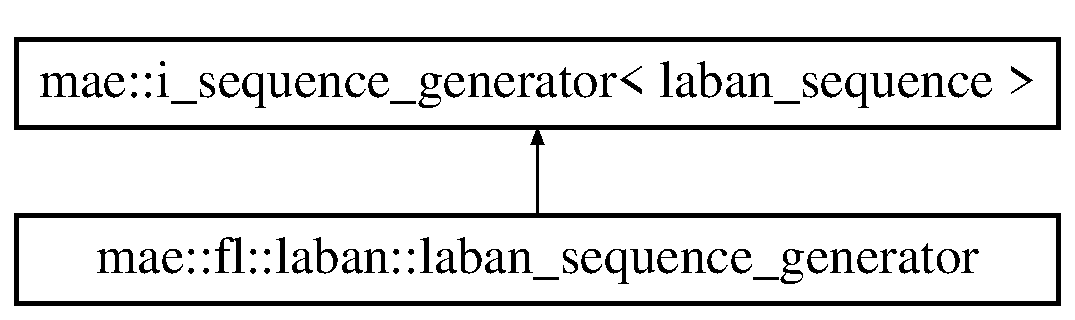
\includegraphics[height=2.000000cm]{classmae_1_1fl_1_1laban_1_1laban__sequence__generator}
\end{center}
\end{figure}
\subsection*{Public Member Functions}
\begin{DoxyCompactItemize}
\item 
\hyperlink{classmae_1_1fl_1_1laban_1_1laban__sequence__generator_a0a792b68242d577bf3a8a627aeeaf43d}{laban\-\_\-sequence\-\_\-generator} (bool debug=false)
\item 
\hyperlink{classmae_1_1fl_1_1laban_1_1laban__sequence__generator_a69a1595e54b58f0051bc9ac8e4c99f82}{laban\-\_\-sequence\-\_\-generator} (std\-::vector$<$ std\-::shared\-\_\-ptr$<$ \hyperlink{classmae_1_1fl_1_1laban_1_1column__definition}{column\-\_\-definition} $>$ $>$ column\-\_\-definitions, unsigned int beats\-\_\-per\-\_\-measure=\hyperlink{classmae_1_1fl_1_1laban_1_1laban__sequence_a2e64362d5cfeb89eb8545cb064e63170}{laban\-\_\-sequence\-::default\-\_\-beats\-\_\-per\-\_\-measure}(), unsigned int beat\-\_\-duration=\hyperlink{classmae_1_1fl_1_1laban_1_1laban__sequence_ac7bf04cdac0c3aed6b8ee4a887e561d9}{laban\-\_\-sequence\-::default\-\_\-beat\-\_\-duration}(), e\-\_\-time\-\_\-unit time\-\_\-unit=\hyperlink{classmae_1_1fl_1_1laban_1_1laban__sequence_ada28215d43d85e983fe6129e9816eed2}{laban\-\_\-sequence\-::default\-\_\-time\-\_\-unit}(), bool debug=false)
\item 
virtual std\-::shared\-\_\-ptr\\*
$<$ \hyperlink{classmae_1_1fl_1_1laban_1_1laban__sequence}{laban\-\_\-sequence} $>$ \hyperlink{classmae_1_1fl_1_1laban_1_1laban__sequence__generator_a6311b99a7bf78c2d9779d601ad88353e}{generate\-\_\-sequence} (double framerate, std\-::list$<$ std\-::shared\-\_\-ptr$<$ \hyperlink{classmae_1_1general__enriched__pose}{general\-\_\-enriched\-\_\-pose} $>$ $>$ key\-\_\-poses, std\-::vector$<$ \hyperlink{classmae_1_1bone}{bone} $>$ body\-\_\-parts)
\end{DoxyCompactItemize}


\subsection{Constructor \& Destructor Documentation}
\hypertarget{classmae_1_1fl_1_1laban_1_1laban__sequence__generator_a0a792b68242d577bf3a8a627aeeaf43d}{\index{mae\-::fl\-::laban\-::laban\-\_\-sequence\-\_\-generator@{mae\-::fl\-::laban\-::laban\-\_\-sequence\-\_\-generator}!laban\-\_\-sequence\-\_\-generator@{laban\-\_\-sequence\-\_\-generator}}
\index{laban\-\_\-sequence\-\_\-generator@{laban\-\_\-sequence\-\_\-generator}!mae::fl::laban::laban_sequence_generator@{mae\-::fl\-::laban\-::laban\-\_\-sequence\-\_\-generator}}
\subsubsection[{laban\-\_\-sequence\-\_\-generator}]{\setlength{\rightskip}{0pt plus 5cm}mae\-::fl\-::laban\-::laban\-\_\-sequence\-\_\-generator\-::laban\-\_\-sequence\-\_\-generator (
\begin{DoxyParamCaption}
\item[{bool}]{debug = {\ttfamily false}}
\end{DoxyParamCaption}
)}}\label{classmae_1_1fl_1_1laban_1_1laban__sequence__generator_a0a792b68242d577bf3a8a627aeeaf43d}
Creates a new sequence generator.


\begin{DoxyParams}{Parameters}
{\em debug} & True if debug output is wanted. \\
\hline
\end{DoxyParams}
\hypertarget{classmae_1_1fl_1_1laban_1_1laban__sequence__generator_a69a1595e54b58f0051bc9ac8e4c99f82}{\index{mae\-::fl\-::laban\-::laban\-\_\-sequence\-\_\-generator@{mae\-::fl\-::laban\-::laban\-\_\-sequence\-\_\-generator}!laban\-\_\-sequence\-\_\-generator@{laban\-\_\-sequence\-\_\-generator}}
\index{laban\-\_\-sequence\-\_\-generator@{laban\-\_\-sequence\-\_\-generator}!mae::fl::laban::laban_sequence_generator@{mae\-::fl\-::laban\-::laban\-\_\-sequence\-\_\-generator}}
\subsubsection[{laban\-\_\-sequence\-\_\-generator}]{\setlength{\rightskip}{0pt plus 5cm}mae\-::fl\-::laban\-::laban\-\_\-sequence\-\_\-generator\-::laban\-\_\-sequence\-\_\-generator (
\begin{DoxyParamCaption}
\item[{std\-::vector$<$ std\-::shared\-\_\-ptr$<$ {\bf column\-\_\-definition} $>$ $>$}]{column\-\_\-definitions, }
\item[{unsigned int}]{beats\-\_\-per\-\_\-measure = {\ttfamily {\bf laban\-\_\-sequence\-::default\-\_\-beats\-\_\-per\-\_\-measure}()}, }
\item[{unsigned int}]{beat\-\_\-duration = {\ttfamily {\bf laban\-\_\-sequence\-::default\-\_\-beat\-\_\-duration}()}, }
\item[{e\-\_\-time\-\_\-unit}]{time\-\_\-unit = {\ttfamily {\bf laban\-\_\-sequence\-::default\-\_\-time\-\_\-unit}()}, }
\item[{bool}]{debug = {\ttfamily false}}
\end{DoxyParamCaption}
)}}\label{classmae_1_1fl_1_1laban_1_1laban__sequence__generator_a69a1595e54b58f0051bc9ac8e4c99f82}
Creates a new sequence generator with additional columns to the default ones.


\begin{DoxyParams}{Parameters}
{\em column\-\_\-definitions} & Column definitions for additional columns. \\
\hline
{\em beats\-\_\-per\-\_\-measure} & The number of beats per measure. \\
\hline
{\em beat\-\_\-duration} & The duration of a single beat given in the time unit. \\
\hline
{\em time\-\_\-unit} & The time unit to be used. \\
\hline
{\em debug} & True if debug output is wanted. \\
\hline
\end{DoxyParams}


\subsection{Member Function Documentation}
\hypertarget{classmae_1_1fl_1_1laban_1_1laban__sequence__generator_a6311b99a7bf78c2d9779d601ad88353e}{\index{mae\-::fl\-::laban\-::laban\-\_\-sequence\-\_\-generator@{mae\-::fl\-::laban\-::laban\-\_\-sequence\-\_\-generator}!generate\-\_\-sequence@{generate\-\_\-sequence}}
\index{generate\-\_\-sequence@{generate\-\_\-sequence}!mae::fl::laban::laban_sequence_generator@{mae\-::fl\-::laban\-::laban\-\_\-sequence\-\_\-generator}}
\subsubsection[{generate\-\_\-sequence}]{\setlength{\rightskip}{0pt plus 5cm}std\-::shared\-\_\-ptr$<$ {\bf laban\-\_\-sequence} $>$ mae\-::fl\-::laban\-::laban\-\_\-sequence\-\_\-generator\-::generate\-\_\-sequence (
\begin{DoxyParamCaption}
\item[{double}]{framerate, }
\item[{std\-::list$<$ std\-::shared\-\_\-ptr$<$ {\bf general\-\_\-enriched\-\_\-pose} $>$ $>$}]{key\-\_\-poses, }
\item[{std\-::vector$<$ {\bf bone} $>$}]{body\-\_\-parts}
\end{DoxyParamCaption}
)\hspace{0.3cm}{\ttfamily [virtual]}}}\label{classmae_1_1fl_1_1laban_1_1laban__sequence__generator_a6311b99a7bf78c2d9779d601ad88353e}
Generates a Labanotation score from the enriched poses.


\begin{DoxyParams}{Parameters}
{\em key\-Poses} & The enriched poses beginning with the lastly performed pose. \\
\hline
{\em body\-\_\-parts} & The addressed body parts. \\
\hline
\end{DoxyParams}
\begin{DoxyReturn}{Returns}
A Labanotation sequence. 
\end{DoxyReturn}


Implements \hyperlink{classmae_1_1i__sequence__generator_a305f7180d41a2b719d9ca36422408e33}{mae\-::i\-\_\-sequence\-\_\-generator$<$ laban\-\_\-sequence $>$}.



The documentation for this class was generated from the following files\-:\begin{DoxyCompactItemize}
\item 
src/mae/fl/laban/laban\-\_\-sequence\-\_\-generator.\-hpp\item 
src/mae/fl/laban/laban\-\_\-sequence\-\_\-generator.\-cpp\end{DoxyCompactItemize}

\hypertarget{classmae_1_1fl_1_1laban_1_1laban__sequence__reader}{\section{mae\-:\-:fl\-:\-:laban\-:\-:laban\-\_\-sequence\-\_\-reader Class Reference}
\label{classmae_1_1fl_1_1laban_1_1laban__sequence__reader}\index{mae\-::fl\-::laban\-::laban\-\_\-sequence\-\_\-reader@{mae\-::fl\-::laban\-::laban\-\_\-sequence\-\_\-reader}}
}
\subsection*{Public Member Functions}
\begin{DoxyCompactItemize}
\item 
\hyperlink{classmae_1_1fl_1_1laban_1_1laban__sequence__reader_a5ec19277963cbbba23c8b9a0e7c46301}{laban\-\_\-sequence\-\_\-reader} ()
\item 
virtual std\-::shared\-\_\-ptr\\*
$<$ \hyperlink{classmae_1_1fl_1_1laban_1_1laban__sequence}{laban\-\_\-sequence} $>$ \hyperlink{classmae_1_1fl_1_1laban_1_1laban__sequence__reader_ae9a04157746544a3b05f96ba42f5f4f7}{read\-\_\-sequence\-\_\-file} (std\-::string file\-\_\-name)
\item 
virtual std\-::shared\-\_\-ptr\\*
$<$ \hyperlink{classmae_1_1fl_1_1laban_1_1laban__sequence}{laban\-\_\-sequence} $>$ \hyperlink{classmae_1_1fl_1_1laban_1_1laban__sequence__reader_a2a073416329826a3be64fdbcccf8ff53}{read\-\_\-sequence\-\_\-str} (std\-::string xml\-\_\-string)
\end{DoxyCompactItemize}


\subsection{Constructor \& Destructor Documentation}
\hypertarget{classmae_1_1fl_1_1laban_1_1laban__sequence__reader_a5ec19277963cbbba23c8b9a0e7c46301}{\index{mae\-::fl\-::laban\-::laban\-\_\-sequence\-\_\-reader@{mae\-::fl\-::laban\-::laban\-\_\-sequence\-\_\-reader}!laban\-\_\-sequence\-\_\-reader@{laban\-\_\-sequence\-\_\-reader}}
\index{laban\-\_\-sequence\-\_\-reader@{laban\-\_\-sequence\-\_\-reader}!mae::fl::laban::laban_sequence_reader@{mae\-::fl\-::laban\-::laban\-\_\-sequence\-\_\-reader}}
\subsubsection[{laban\-\_\-sequence\-\_\-reader}]{\setlength{\rightskip}{0pt plus 5cm}mae\-::fl\-::laban\-::laban\-\_\-sequence\-\_\-reader\-::laban\-\_\-sequence\-\_\-reader (
\begin{DoxyParamCaption}
{}
\end{DoxyParamCaption}
)}}\label{classmae_1_1fl_1_1laban_1_1laban__sequence__reader_a5ec19277963cbbba23c8b9a0e7c46301}
Creates a new laban sequence reader. 

\subsection{Member Function Documentation}
\hypertarget{classmae_1_1fl_1_1laban_1_1laban__sequence__reader_ae9a04157746544a3b05f96ba42f5f4f7}{\index{mae\-::fl\-::laban\-::laban\-\_\-sequence\-\_\-reader@{mae\-::fl\-::laban\-::laban\-\_\-sequence\-\_\-reader}!read\-\_\-sequence\-\_\-file@{read\-\_\-sequence\-\_\-file}}
\index{read\-\_\-sequence\-\_\-file@{read\-\_\-sequence\-\_\-file}!mae::fl::laban::laban_sequence_reader@{mae\-::fl\-::laban\-::laban\-\_\-sequence\-\_\-reader}}
\subsubsection[{read\-\_\-sequence\-\_\-file}]{\setlength{\rightskip}{0pt plus 5cm}std\-::shared\-\_\-ptr$<$ {\bf laban\-\_\-sequence} $>$ mae\-::fl\-::laban\-::laban\-\_\-sequence\-\_\-reader\-::read\-\_\-sequence\-\_\-file (
\begin{DoxyParamCaption}
\item[{std\-::string}]{file\-\_\-name}
\end{DoxyParamCaption}
)\hspace{0.3cm}{\ttfamily [virtual]}}}\label{classmae_1_1fl_1_1laban_1_1laban__sequence__reader_ae9a04157746544a3b05f96ba42f5f4f7}
Reads the Labanotation X\-M\-L (which is defined by the Labanotation X\-M\-L schema v.\-0.\-5) file and generates a sequence of it.


\begin{DoxyParams}{Parameters}
{\em xml\-\_\-string} & The path to the X\-M\-L file. \\
\hline
\end{DoxyParams}
\begin{DoxyReturn}{Returns}
A shared pointer to the sequence. 
\end{DoxyReturn}
\hypertarget{classmae_1_1fl_1_1laban_1_1laban__sequence__reader_a2a073416329826a3be64fdbcccf8ff53}{\index{mae\-::fl\-::laban\-::laban\-\_\-sequence\-\_\-reader@{mae\-::fl\-::laban\-::laban\-\_\-sequence\-\_\-reader}!read\-\_\-sequence\-\_\-str@{read\-\_\-sequence\-\_\-str}}
\index{read\-\_\-sequence\-\_\-str@{read\-\_\-sequence\-\_\-str}!mae::fl::laban::laban_sequence_reader@{mae\-::fl\-::laban\-::laban\-\_\-sequence\-\_\-reader}}
\subsubsection[{read\-\_\-sequence\-\_\-str}]{\setlength{\rightskip}{0pt plus 5cm}std\-::shared\-\_\-ptr$<$ {\bf laban\-\_\-sequence} $>$ mae\-::fl\-::laban\-::laban\-\_\-sequence\-\_\-reader\-::read\-\_\-sequence\-\_\-str (
\begin{DoxyParamCaption}
\item[{std\-::string}]{xml\-\_\-string}
\end{DoxyParamCaption}
)\hspace{0.3cm}{\ttfamily [virtual]}}}\label{classmae_1_1fl_1_1laban_1_1laban__sequence__reader_a2a073416329826a3be64fdbcccf8ff53}
Reads the Labanotation X\-M\-L (which is defined by the Labanotation X\-M\-L schema v.\-0.\-5) string and generates a sequence of it. The string should contain the whole X\-M\-L part which is validated against the X\-M\-L schema.


\begin{DoxyParams}{Parameters}
{\em xml\-\_\-string} & The X\-M\-L string. \\
\hline
\end{DoxyParams}
\begin{DoxyReturn}{Returns}
A shared pointer to the sequence. 
\end{DoxyReturn}


The documentation for this class was generated from the following files\-:\begin{DoxyCompactItemize}
\item 
src/mae/fl/laban/laban\-\_\-sequence\-\_\-reader.\-hpp\item 
src/mae/fl/laban/laban\-\_\-sequence\-\_\-reader.\-cpp\end{DoxyCompactItemize}

\hypertarget{classmae_1_1fl_1_1laban_1_1laban__sequence__recognizer}{\section{mae\-:\-:fl\-:\-:laban\-:\-:laban\-\_\-sequence\-\_\-recognizer Class Reference}
\label{classmae_1_1fl_1_1laban_1_1laban__sequence__recognizer}\index{mae\-::fl\-::laban\-::laban\-\_\-sequence\-\_\-recognizer@{mae\-::fl\-::laban\-::laban\-\_\-sequence\-\_\-recognizer}}
}
Inheritance diagram for mae\-:\-:fl\-:\-:laban\-:\-:laban\-\_\-sequence\-\_\-recognizer\-:\begin{figure}[H]
\begin{center}
\leavevmode
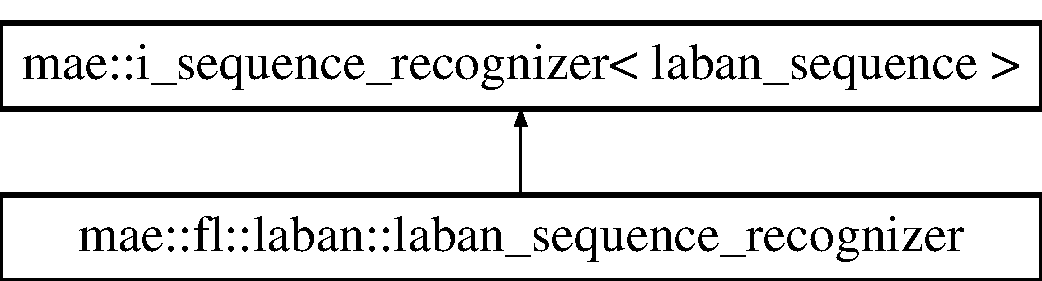
\includegraphics[height=2.000000cm]{classmae_1_1fl_1_1laban_1_1laban__sequence__recognizer}
\end{center}
\end{figure}
\subsection*{Public Member Functions}
\begin{DoxyCompactItemize}
\item 
\hyperlink{classmae_1_1fl_1_1laban_1_1laban__sequence__recognizer_ac8bcf4bda67c74efb755aaac707def33}{laban\-\_\-sequence\-\_\-recognizer} (bool debug=false)
\item 
\hyperlink{classmae_1_1fl_1_1laban_1_1laban__sequence__recognizer_a74b400fd80ee4dd76588a0e938a6adc6}{laban\-\_\-sequence\-\_\-recognizer} (std\-::vector$<$ std\-::shared\-\_\-ptr$<$ \hyperlink{classmae_1_1fl_1_1laban_1_1column__definition}{column\-\_\-definition} $>$ $>$ column\-\_\-definitions, unsigned int beats\-\_\-per\-\_\-measure=\hyperlink{classmae_1_1fl_1_1laban_1_1laban__sequence_a2e64362d5cfeb89eb8545cb064e63170}{laban\-\_\-sequence\-::default\-\_\-beats\-\_\-per\-\_\-measure}(), unsigned int beat\-\_\-duration=\hyperlink{classmae_1_1fl_1_1laban_1_1laban__sequence_ac7bf04cdac0c3aed6b8ee4a887e561d9}{laban\-\_\-sequence\-::default\-\_\-beat\-\_\-duration}(), e\-\_\-time\-\_\-unit time\-\_\-unit=\hyperlink{classmae_1_1fl_1_1laban_1_1laban__sequence_ada28215d43d85e983fe6129e9816eed2}{laban\-\_\-sequence\-::default\-\_\-time\-\_\-unit}(), bool debug=false)
\item 
virtual void \hyperlink{classmae_1_1fl_1_1laban_1_1laban__sequence__recognizer_a2a6255ac083530269ca80a74c1b01a68}{set\-\_\-recognition\-\_\-tolerance} (double tolerance)
\item 
virtual std\-::shared\-\_\-ptr\\*
$<$ \hyperlink{classmae_1_1fl_1_1laban_1_1decision__forest}{decision\-\_\-forest} $>$ \hyperlink{classmae_1_1fl_1_1laban_1_1laban__sequence__recognizer_a3d4b0585fa58c25df6b6f70eff922cc2}{get\-\_\-decision\-\_\-forest} ()
\item 
virtual void \hyperlink{classmae_1_1fl_1_1laban_1_1laban__sequence__recognizer_a5275a3620709af2f4ff984382029a89e}{register\-\_\-sequence} (std\-::shared\-\_\-ptr$<$ \hyperlink{classmae_1_1fl_1_1laban_1_1laban__sequence}{laban\-\_\-sequence} $>$ sequence)
\item 
virtual bool \hyperlink{classmae_1_1fl_1_1laban_1_1laban__sequence__recognizer_a31410c5237b11f78e0ecdbc664157adf}{deregister\-\_\-sequence} (std\-::shared\-\_\-ptr$<$ \hyperlink{classmae_1_1fl_1_1laban_1_1laban__sequence}{laban\-\_\-sequence} $>$ sequence)
\item 
virtual bool \hyperlink{classmae_1_1fl_1_1laban_1_1laban__sequence__recognizer_ac3fb568e668228472ea3a1ff0124898e}{deregister\-\_\-sequence} (unsigned int list\-\_\-index)
\item 
virtual void \hyperlink{classmae_1_1fl_1_1laban_1_1laban__sequence__recognizer_a4eaa30d1cd8064e381765a2b3385a248}{clear\-\_\-registered\-\_\-sequences} ()
\item 
virtual std\-::list\\*
$<$ std\-::shared\-\_\-ptr\\*
$<$ \hyperlink{classmae_1_1fl_1_1laban_1_1laban__sequence}{laban\-\_\-sequence} $>$ $>$ \hyperlink{classmae_1_1fl_1_1laban_1_1laban__sequence__recognizer_ae7d217b9a173ae7c8c755856d73113f3}{get\-\_\-registered\-\_\-sequences} ()
\item 
virtual int \hyperlink{classmae_1_1fl_1_1laban_1_1laban__sequence__recognizer_a4cb477435572ac7f3c30f8ddc22587a8}{get\-\_\-sequence\-\_\-length} (std\-::shared\-\_\-ptr$<$ \hyperlink{classmae_1_1fl_1_1laban_1_1laban__sequence}{laban\-\_\-sequence} $>$ sequence)
\item 
virtual std\-::vector\\*
$<$ std\-::shared\-\_\-ptr\\*
$<$ \hyperlink{classmae_1_1fl_1_1laban_1_1laban__sequence}{laban\-\_\-sequence} $>$ $>$ \hyperlink{classmae_1_1fl_1_1laban_1_1laban__sequence__recognizer_afd0fe4b625602a5b169095a3e367349d}{recognize\-\_\-sequence} (std\-::shared\-\_\-ptr$<$ \hyperlink{classmae_1_1fl_1_1laban_1_1laban__sequence}{laban\-\_\-sequence} $>$ sequence, std\-::vector$<$ \hyperlink{classmae_1_1bone}{bone} $>$ body\-\_\-parts)
\item 
virtual std\-::string \hyperlink{classmae_1_1fl_1_1laban_1_1laban__sequence__recognizer_af411c388147b6945827ab7fdd47ce131}{str} () const 
\end{DoxyCompactItemize}


\subsection{Constructor \& Destructor Documentation}
\hypertarget{classmae_1_1fl_1_1laban_1_1laban__sequence__recognizer_ac8bcf4bda67c74efb755aaac707def33}{\index{mae\-::fl\-::laban\-::laban\-\_\-sequence\-\_\-recognizer@{mae\-::fl\-::laban\-::laban\-\_\-sequence\-\_\-recognizer}!laban\-\_\-sequence\-\_\-recognizer@{laban\-\_\-sequence\-\_\-recognizer}}
\index{laban\-\_\-sequence\-\_\-recognizer@{laban\-\_\-sequence\-\_\-recognizer}!mae::fl::laban::laban_sequence_recognizer@{mae\-::fl\-::laban\-::laban\-\_\-sequence\-\_\-recognizer}}
\subsubsection[{laban\-\_\-sequence\-\_\-recognizer}]{\setlength{\rightskip}{0pt plus 5cm}mae\-::fl\-::laban\-::laban\-\_\-sequence\-\_\-recognizer\-::laban\-\_\-sequence\-\_\-recognizer (
\begin{DoxyParamCaption}
\item[{bool}]{debug = {\ttfamily false}}
\end{DoxyParamCaption}
)}}\label{classmae_1_1fl_1_1laban_1_1laban__sequence__recognizer_ac8bcf4bda67c74efb755aaac707def33}
Creates a new recognizer for laban sequences.


\begin{DoxyParams}{Parameters}
{\em debug} & True for debug output on the terminal. \\
\hline
\end{DoxyParams}
\hypertarget{classmae_1_1fl_1_1laban_1_1laban__sequence__recognizer_a74b400fd80ee4dd76588a0e938a6adc6}{\index{mae\-::fl\-::laban\-::laban\-\_\-sequence\-\_\-recognizer@{mae\-::fl\-::laban\-::laban\-\_\-sequence\-\_\-recognizer}!laban\-\_\-sequence\-\_\-recognizer@{laban\-\_\-sequence\-\_\-recognizer}}
\index{laban\-\_\-sequence\-\_\-recognizer@{laban\-\_\-sequence\-\_\-recognizer}!mae::fl::laban::laban_sequence_recognizer@{mae\-::fl\-::laban\-::laban\-\_\-sequence\-\_\-recognizer}}
\subsubsection[{laban\-\_\-sequence\-\_\-recognizer}]{\setlength{\rightskip}{0pt plus 5cm}mae\-::fl\-::laban\-::laban\-\_\-sequence\-\_\-recognizer\-::laban\-\_\-sequence\-\_\-recognizer (
\begin{DoxyParamCaption}
\item[{std\-::vector$<$ std\-::shared\-\_\-ptr$<$ {\bf column\-\_\-definition} $>$ $>$}]{column\-\_\-definitions, }
\item[{unsigned int}]{beats\-\_\-per\-\_\-measure = {\ttfamily {\bf laban\-\_\-sequence\-::default\-\_\-beats\-\_\-per\-\_\-measure}()}, }
\item[{unsigned int}]{beat\-\_\-duration = {\ttfamily {\bf laban\-\_\-sequence\-::default\-\_\-beat\-\_\-duration}()}, }
\item[{e\-\_\-time\-\_\-unit}]{time\-\_\-unit = {\ttfamily {\bf laban\-\_\-sequence\-::default\-\_\-time\-\_\-unit}()}, }
\item[{bool}]{debug = {\ttfamily false}}
\end{DoxyParamCaption}
)}}\label{classmae_1_1fl_1_1laban_1_1laban__sequence__recognizer_a74b400fd80ee4dd76588a0e938a6adc6}
Creates a new recognizer for laban sequences.


\begin{DoxyParams}{Parameters}
{\em column\-\_\-definitions} & The column definitions as used by the laban sequence generator. \\
\hline
{\em beats\-\_\-per\-\_\-measure} & The number of beats per measure as used by the laban sequence generator. \\
\hline
{\em beat\-\_\-duration} & The beat duration as used by the laban sequence generator. \\
\hline
{\em time\-\_\-unit} & The time unit as used by the laban sequence generator. \\
\hline
{\em debug} & True for debug output on the terminal. \\
\hline
\end{DoxyParams}


\subsection{Member Function Documentation}
\hypertarget{classmae_1_1fl_1_1laban_1_1laban__sequence__recognizer_a4eaa30d1cd8064e381765a2b3385a248}{\index{mae\-::fl\-::laban\-::laban\-\_\-sequence\-\_\-recognizer@{mae\-::fl\-::laban\-::laban\-\_\-sequence\-\_\-recognizer}!clear\-\_\-registered\-\_\-sequences@{clear\-\_\-registered\-\_\-sequences}}
\index{clear\-\_\-registered\-\_\-sequences@{clear\-\_\-registered\-\_\-sequences}!mae::fl::laban::laban_sequence_recognizer@{mae\-::fl\-::laban\-::laban\-\_\-sequence\-\_\-recognizer}}
\subsubsection[{clear\-\_\-registered\-\_\-sequences}]{\setlength{\rightskip}{0pt plus 5cm}void mae\-::fl\-::laban\-::laban\-\_\-sequence\-\_\-recognizer\-::clear\-\_\-registered\-\_\-sequences (
\begin{DoxyParamCaption}
{}
\end{DoxyParamCaption}
)\hspace{0.3cm}{\ttfamily [virtual]}}}\label{classmae_1_1fl_1_1laban_1_1laban__sequence__recognizer_a4eaa30d1cd8064e381765a2b3385a248}
Removes all registered sequences. 

Implements \hyperlink{classmae_1_1i__sequence__recognizer}{mae\-::i\-\_\-sequence\-\_\-recognizer$<$ laban\-\_\-sequence $>$}.

\hypertarget{classmae_1_1fl_1_1laban_1_1laban__sequence__recognizer_a31410c5237b11f78e0ecdbc664157adf}{\index{mae\-::fl\-::laban\-::laban\-\_\-sequence\-\_\-recognizer@{mae\-::fl\-::laban\-::laban\-\_\-sequence\-\_\-recognizer}!deregister\-\_\-sequence@{deregister\-\_\-sequence}}
\index{deregister\-\_\-sequence@{deregister\-\_\-sequence}!mae::fl::laban::laban_sequence_recognizer@{mae\-::fl\-::laban\-::laban\-\_\-sequence\-\_\-recognizer}}
\subsubsection[{deregister\-\_\-sequence}]{\setlength{\rightskip}{0pt plus 5cm}bool mae\-::fl\-::laban\-::laban\-\_\-sequence\-\_\-recognizer\-::deregister\-\_\-sequence (
\begin{DoxyParamCaption}
\item[{std\-::shared\-\_\-ptr$<$ {\bf laban\-\_\-sequence} $>$}]{sequence}
\end{DoxyParamCaption}
)\hspace{0.3cm}{\ttfamily [virtual]}}}\label{classmae_1_1fl_1_1laban_1_1laban__sequence__recognizer_a31410c5237b11f78e0ecdbc664157adf}
Removes the sequence from the recognizer.


\begin{DoxyParams}{Parameters}
{\em sequence} & The sequence. \\
\hline
\end{DoxyParams}
\begin{DoxyReturn}{Returns}
True if the sequence was removed. 
\end{DoxyReturn}
\hypertarget{classmae_1_1fl_1_1laban_1_1laban__sequence__recognizer_ac3fb568e668228472ea3a1ff0124898e}{\index{mae\-::fl\-::laban\-::laban\-\_\-sequence\-\_\-recognizer@{mae\-::fl\-::laban\-::laban\-\_\-sequence\-\_\-recognizer}!deregister\-\_\-sequence@{deregister\-\_\-sequence}}
\index{deregister\-\_\-sequence@{deregister\-\_\-sequence}!mae::fl::laban::laban_sequence_recognizer@{mae\-::fl\-::laban\-::laban\-\_\-sequence\-\_\-recognizer}}
\subsubsection[{deregister\-\_\-sequence}]{\setlength{\rightskip}{0pt plus 5cm}bool mae\-::fl\-::laban\-::laban\-\_\-sequence\-\_\-recognizer\-::deregister\-\_\-sequence (
\begin{DoxyParamCaption}
\item[{unsigned int}]{list\-\_\-index}
\end{DoxyParamCaption}
)\hspace{0.3cm}{\ttfamily [virtual]}}}\label{classmae_1_1fl_1_1laban_1_1laban__sequence__recognizer_ac3fb568e668228472ea3a1ff0124898e}
Removes the sequence at the index position of the list.


\begin{DoxyParams}{Parameters}
{\em list\-\_\-index} & The index. \\
\hline
\end{DoxyParams}
\begin{DoxyReturn}{Returns}
True if the sequence was removed. 
\end{DoxyReturn}


Implements \hyperlink{classmae_1_1i__sequence__recognizer}{mae\-::i\-\_\-sequence\-\_\-recognizer$<$ laban\-\_\-sequence $>$}.

\hypertarget{classmae_1_1fl_1_1laban_1_1laban__sequence__recognizer_a3d4b0585fa58c25df6b6f70eff922cc2}{\index{mae\-::fl\-::laban\-::laban\-\_\-sequence\-\_\-recognizer@{mae\-::fl\-::laban\-::laban\-\_\-sequence\-\_\-recognizer}!get\-\_\-decision\-\_\-forest@{get\-\_\-decision\-\_\-forest}}
\index{get\-\_\-decision\-\_\-forest@{get\-\_\-decision\-\_\-forest}!mae::fl::laban::laban_sequence_recognizer@{mae\-::fl\-::laban\-::laban\-\_\-sequence\-\_\-recognizer}}
\subsubsection[{get\-\_\-decision\-\_\-forest}]{\setlength{\rightskip}{0pt plus 5cm}std\-::shared\-\_\-ptr$<$ {\bf decision\-\_\-forest} $>$ mae\-::fl\-::laban\-::laban\-\_\-sequence\-\_\-recognizer\-::get\-\_\-decision\-\_\-forest (
\begin{DoxyParamCaption}
{}
\end{DoxyParamCaption}
)\hspace{0.3cm}{\ttfamily [virtual]}}}\label{classmae_1_1fl_1_1laban_1_1laban__sequence__recognizer_a3d4b0585fa58c25df6b6f70eff922cc2}
Returns the underlying decision forest used to recognize sequences.

\begin{DoxyReturn}{Returns}
The decision forest. 
\end{DoxyReturn}
\hypertarget{classmae_1_1fl_1_1laban_1_1laban__sequence__recognizer_ae7d217b9a173ae7c8c755856d73113f3}{\index{mae\-::fl\-::laban\-::laban\-\_\-sequence\-\_\-recognizer@{mae\-::fl\-::laban\-::laban\-\_\-sequence\-\_\-recognizer}!get\-\_\-registered\-\_\-sequences@{get\-\_\-registered\-\_\-sequences}}
\index{get\-\_\-registered\-\_\-sequences@{get\-\_\-registered\-\_\-sequences}!mae::fl::laban::laban_sequence_recognizer@{mae\-::fl\-::laban\-::laban\-\_\-sequence\-\_\-recognizer}}
\subsubsection[{get\-\_\-registered\-\_\-sequences}]{\setlength{\rightskip}{0pt plus 5cm}std\-::list$<$ std\-::shared\-\_\-ptr$<$ {\bf laban\-\_\-sequence} $>$ $>$ mae\-::fl\-::laban\-::laban\-\_\-sequence\-\_\-recognizer\-::get\-\_\-registered\-\_\-sequences (
\begin{DoxyParamCaption}
{}
\end{DoxyParamCaption}
)\hspace{0.3cm}{\ttfamily [virtual]}}}\label{classmae_1_1fl_1_1laban_1_1laban__sequence__recognizer_ae7d217b9a173ae7c8c755856d73113f3}
Returns all registered sequences.

\begin{DoxyReturn}{Returns}
All sequences. 
\end{DoxyReturn}
\hypertarget{classmae_1_1fl_1_1laban_1_1laban__sequence__recognizer_a4cb477435572ac7f3c30f8ddc22587a8}{\index{mae\-::fl\-::laban\-::laban\-\_\-sequence\-\_\-recognizer@{mae\-::fl\-::laban\-::laban\-\_\-sequence\-\_\-recognizer}!get\-\_\-sequence\-\_\-length@{get\-\_\-sequence\-\_\-length}}
\index{get\-\_\-sequence\-\_\-length@{get\-\_\-sequence\-\_\-length}!mae::fl::laban::laban_sequence_recognizer@{mae\-::fl\-::laban\-::laban\-\_\-sequence\-\_\-recognizer}}
\subsubsection[{get\-\_\-sequence\-\_\-length}]{\setlength{\rightskip}{0pt plus 5cm}int mae\-::fl\-::laban\-::laban\-\_\-sequence\-\_\-recognizer\-::get\-\_\-sequence\-\_\-length (
\begin{DoxyParamCaption}
\item[{std\-::shared\-\_\-ptr$<$ {\bf laban\-\_\-sequence} $>$}]{sequence}
\end{DoxyParamCaption}
)\hspace{0.3cm}{\ttfamily [virtual]}}}\label{classmae_1_1fl_1_1laban_1_1laban__sequence__recognizer_a4cb477435572ac7f3c30f8ddc22587a8}
Returns the length of the sequence in milliseconds.


\begin{DoxyParams}{Parameters}
{\em sequence} & The sequence. \\
\hline
\end{DoxyParams}
\begin{DoxyReturn}{Returns}
The length of the sequence. 
\end{DoxyReturn}
\hypertarget{classmae_1_1fl_1_1laban_1_1laban__sequence__recognizer_afd0fe4b625602a5b169095a3e367349d}{\index{mae\-::fl\-::laban\-::laban\-\_\-sequence\-\_\-recognizer@{mae\-::fl\-::laban\-::laban\-\_\-sequence\-\_\-recognizer}!recognize\-\_\-sequence@{recognize\-\_\-sequence}}
\index{recognize\-\_\-sequence@{recognize\-\_\-sequence}!mae::fl::laban::laban_sequence_recognizer@{mae\-::fl\-::laban\-::laban\-\_\-sequence\-\_\-recognizer}}
\subsubsection[{recognize\-\_\-sequence}]{\setlength{\rightskip}{0pt plus 5cm}std\-::vector$<$ std\-::shared\-\_\-ptr$<$ {\bf laban\-\_\-sequence} $>$ $>$ mae\-::fl\-::laban\-::laban\-\_\-sequence\-\_\-recognizer\-::recognize\-\_\-sequence (
\begin{DoxyParamCaption}
\item[{std\-::shared\-\_\-ptr$<$ {\bf laban\-\_\-sequence} $>$}]{sequence, }
\item[{std\-::vector$<$ {\bf bone} $>$}]{body\-\_\-parts}
\end{DoxyParamCaption}
)\hspace{0.3cm}{\ttfamily [virtual]}}}\label{classmae_1_1fl_1_1laban_1_1laban__sequence__recognizer_afd0fe4b625602a5b169095a3e367349d}
Recognized subsequences in the sequence for the given body parts.


\begin{DoxyParams}{Parameters}
{\em sequence} & The sequences to be looked at. \\
\hline
{\em body\-\_\-parts} & The body parts. \\
\hline
\end{DoxyParams}
\begin{DoxyReturn}{Returns}
All matches. 
\end{DoxyReturn}
\hypertarget{classmae_1_1fl_1_1laban_1_1laban__sequence__recognizer_a5275a3620709af2f4ff984382029a89e}{\index{mae\-::fl\-::laban\-::laban\-\_\-sequence\-\_\-recognizer@{mae\-::fl\-::laban\-::laban\-\_\-sequence\-\_\-recognizer}!register\-\_\-sequence@{register\-\_\-sequence}}
\index{register\-\_\-sequence@{register\-\_\-sequence}!mae::fl::laban::laban_sequence_recognizer@{mae\-::fl\-::laban\-::laban\-\_\-sequence\-\_\-recognizer}}
\subsubsection[{register\-\_\-sequence}]{\setlength{\rightskip}{0pt plus 5cm}void mae\-::fl\-::laban\-::laban\-\_\-sequence\-\_\-recognizer\-::register\-\_\-sequence (
\begin{DoxyParamCaption}
\item[{std\-::shared\-\_\-ptr$<$ {\bf laban\-\_\-sequence} $>$}]{sequence}
\end{DoxyParamCaption}
)\hspace{0.3cm}{\ttfamily [virtual]}}}\label{classmae_1_1fl_1_1laban_1_1laban__sequence__recognizer_a5275a3620709af2f4ff984382029a89e}
Registers a sequence to the recognizer.


\begin{DoxyParams}{Parameters}
{\em sequence} & The sequence. \\
\hline
\end{DoxyParams}
\hypertarget{classmae_1_1fl_1_1laban_1_1laban__sequence__recognizer_a2a6255ac083530269ca80a74c1b01a68}{\index{mae\-::fl\-::laban\-::laban\-\_\-sequence\-\_\-recognizer@{mae\-::fl\-::laban\-::laban\-\_\-sequence\-\_\-recognizer}!set\-\_\-recognition\-\_\-tolerance@{set\-\_\-recognition\-\_\-tolerance}}
\index{set\-\_\-recognition\-\_\-tolerance@{set\-\_\-recognition\-\_\-tolerance}!mae::fl::laban::laban_sequence_recognizer@{mae\-::fl\-::laban\-::laban\-\_\-sequence\-\_\-recognizer}}
\subsubsection[{set\-\_\-recognition\-\_\-tolerance}]{\setlength{\rightskip}{0pt plus 5cm}void mae\-::fl\-::laban\-::laban\-\_\-sequence\-\_\-recognizer\-::set\-\_\-recognition\-\_\-tolerance (
\begin{DoxyParamCaption}
\item[{double}]{tolerance}
\end{DoxyParamCaption}
)\hspace{0.3cm}{\ttfamily [virtual]}}}\label{classmae_1_1fl_1_1laban_1_1laban__sequence__recognizer_a2a6255ac083530269ca80a74c1b01a68}
Sets the tolerance for the recognition. The tolerance is a value which represents the number of beats of the labanotation which are tolerated in deviation.


\begin{DoxyParams}{Parameters}
{\em tolerance} & The tolerance to be accepted. \\
\hline
\end{DoxyParams}
\hypertarget{classmae_1_1fl_1_1laban_1_1laban__sequence__recognizer_af411c388147b6945827ab7fdd47ce131}{\index{mae\-::fl\-::laban\-::laban\-\_\-sequence\-\_\-recognizer@{mae\-::fl\-::laban\-::laban\-\_\-sequence\-\_\-recognizer}!str@{str}}
\index{str@{str}!mae::fl::laban::laban_sequence_recognizer@{mae\-::fl\-::laban\-::laban\-\_\-sequence\-\_\-recognizer}}
\subsubsection[{str}]{\setlength{\rightskip}{0pt plus 5cm}std\-::string mae\-::fl\-::laban\-::laban\-\_\-sequence\-\_\-recognizer\-::str (
\begin{DoxyParamCaption}
{}
\end{DoxyParamCaption}
) const\hspace{0.3cm}{\ttfamily [virtual]}}}\label{classmae_1_1fl_1_1laban_1_1laban__sequence__recognizer_af411c388147b6945827ab7fdd47ce131}
Returns the string representation for the underlying decision forest.

\begin{DoxyReturn}{Returns}
The string. 
\end{DoxyReturn}


The documentation for this class was generated from the following files\-:\begin{DoxyCompactItemize}
\item 
src/mae/fl/laban/laban\-\_\-sequence\-\_\-recognizer.\-hpp\item 
src/mae/fl/laban/laban\-\_\-sequence\-\_\-recognizer.\-cpp\end{DoxyCompactItemize}

\hypertarget{classmae_1_1math_1_1math}{\section{mae\-:\-:math\-:\-:math Class Reference}
\label{classmae_1_1math_1_1math}\index{mae\-::math\-::math@{mae\-::math\-::math}}
}
\subsection*{Static Public Member Functions}
\begin{DoxyCompactItemize}
\item 
static std\-::shared\-\_\-ptr$<$ \hyperlink{classmae_1_1math_1_1vec3d}{vec3d} $>$ \hyperlink{classmae_1_1math_1_1math_a31f87c06fdc0ba609e3dd96154fdd9f2}{project\-\_\-to\-\_\-basis} (std\-::shared\-\_\-ptr$<$ \hyperlink{classmae_1_1math_1_1vec3d}{vec3d} $>$ point, std\-::shared\-\_\-ptr$<$ \hyperlink{classmae_1_1math_1_1basis}{basis} $>$ \hyperlink{classmae_1_1math_1_1basis}{basis}, std\-::shared\-\_\-ptr$<$ \hyperlink{classmae_1_1math_1_1vec3d}{vec3d} $>$ position\-\_\-vector=nullptr)
\item 
static std\-::shared\-\_\-ptr$<$ \hyperlink{classmae_1_1math_1_1vec3d}{vec3d} $>$ \hyperlink{classmae_1_1math_1_1math_a889e4a757fe5237fb55995c013224da9}{project\-\_\-back\-\_\-to\-\_\-default} (std\-::shared\-\_\-ptr$<$ \hyperlink{classmae_1_1math_1_1vec3d}{vec3d} $>$ point, std\-::shared\-\_\-ptr$<$ \hyperlink{classmae_1_1math_1_1basis}{basis} $>$ \hyperlink{classmae_1_1math_1_1basis}{basis}, std\-::shared\-\_\-ptr$<$ \hyperlink{classmae_1_1math_1_1vec3d}{vec3d} $>$ position\-\_\-vector=nullptr)
\item 
static double \hyperlink{classmae_1_1math_1_1math_a37ab34ed5a6b7b7253dc7657e2b3a5ea}{rad\-\_\-to\-\_\-deg} (double val)
\item 
static double \hyperlink{classmae_1_1math_1_1math_a87dfc60d31b86942b9147377bef659f5}{deg\-\_\-to\-\_\-rad} (double val)
\item 
static bool \hyperlink{classmae_1_1math_1_1math_a5f5bfb261b612865655ec615d1927b43}{are\-\_\-collinear} (std\-::shared\-\_\-ptr$<$ \hyperlink{classmae_1_1math_1_1vec3d}{vec3d} $>$ a, std\-::shared\-\_\-ptr$<$ \hyperlink{classmae_1_1math_1_1vec3d}{vec3d} $>$ b)
\item 
static double \hyperlink{classmae_1_1math_1_1math_a056dea5a5dd1f865e9ebc5241450b817}{calc\-\_\-angle\-\_\-plane} (std\-::shared\-\_\-ptr$<$ \hyperlink{classmae_1_1math_1_1vec3d}{vec3d} $>$ a, std\-::shared\-\_\-ptr$<$ \hyperlink{classmae_1_1math_1_1vec3d}{vec3d} $>$ b, std\-::shared\-\_\-ptr$<$ \hyperlink{classmae_1_1math_1_1vec3d}{vec3d} $>$ normal)
\item 
static double \hyperlink{classmae_1_1math_1_1math_a1ea721c79b805ed2306da4fe2db47240}{calc\-\_\-angle\-\_\-plane\-\_\-deg} (std\-::shared\-\_\-ptr$<$ \hyperlink{classmae_1_1math_1_1vec3d}{vec3d} $>$ a, std\-::shared\-\_\-ptr$<$ \hyperlink{classmae_1_1math_1_1vec3d}{vec3d} $>$ b, std\-::shared\-\_\-ptr$<$ \hyperlink{classmae_1_1math_1_1vec3d}{vec3d} $>$ normal)
\item 
static double \hyperlink{classmae_1_1math_1_1math_a5e900d86051515004b6d0bd2320c9fd0}{calc\-\_\-angle\-\_\-half} (std\-::shared\-\_\-ptr$<$ \hyperlink{classmae_1_1math_1_1vec3d}{vec3d} $>$ a, std\-::shared\-\_\-ptr$<$ \hyperlink{classmae_1_1math_1_1vec3d}{vec3d} $>$ b)
\item 
static double \hyperlink{classmae_1_1math_1_1math_a6c1cd5db044186f80df86511ba0108da}{calc\-\_\-angle\-\_\-half\-\_\-deg} (std\-::shared\-\_\-ptr$<$ \hyperlink{classmae_1_1math_1_1vec3d}{vec3d} $>$ a, std\-::shared\-\_\-ptr$<$ \hyperlink{classmae_1_1math_1_1vec3d}{vec3d} $>$ b)
\item 
static double \hyperlink{classmae_1_1math_1_1math_a7e7a0068fe2cb5dd78f3df81cd082cb7}{fmod\-\_\-pos} (double a, double b)
\item 
static int \hyperlink{classmae_1_1math_1_1math_a80bbc1acd22c10f1fc69ea41f95304f3}{sign} (double x)
\end{DoxyCompactItemize}


\subsection{Member Function Documentation}
\hypertarget{classmae_1_1math_1_1math_a5f5bfb261b612865655ec615d1927b43}{\index{mae\-::math\-::math@{mae\-::math\-::math}!are\-\_\-collinear@{are\-\_\-collinear}}
\index{are\-\_\-collinear@{are\-\_\-collinear}!mae::math::math@{mae\-::math\-::math}}
\subsubsection[{are\-\_\-collinear}]{\setlength{\rightskip}{0pt plus 5cm}bool mae\-::math\-::math\-::are\-\_\-collinear (
\begin{DoxyParamCaption}
\item[{std\-::shared\-\_\-ptr$<$ {\bf vec3d} $>$}]{a, }
\item[{std\-::shared\-\_\-ptr$<$ {\bf vec3d} $>$}]{b}
\end{DoxyParamCaption}
)\hspace{0.3cm}{\ttfamily [static]}}}\label{classmae_1_1math_1_1math_a5f5bfb261b612865655ec615d1927b43}
Returns true if the vectors are approximately collinear.


\begin{DoxyParams}{Parameters}
{\em a} & The vector a. \\
\hline
{\em b} & The vector a. \\
\hline
\end{DoxyParams}
\begin{DoxyReturn}{Returns}
True if collinear. 
\end{DoxyReturn}
\hypertarget{classmae_1_1math_1_1math_a5e900d86051515004b6d0bd2320c9fd0}{\index{mae\-::math\-::math@{mae\-::math\-::math}!calc\-\_\-angle\-\_\-half@{calc\-\_\-angle\-\_\-half}}
\index{calc\-\_\-angle\-\_\-half@{calc\-\_\-angle\-\_\-half}!mae::math::math@{mae\-::math\-::math}}
\subsubsection[{calc\-\_\-angle\-\_\-half}]{\setlength{\rightskip}{0pt plus 5cm}double mae\-::math\-::math\-::calc\-\_\-angle\-\_\-half (
\begin{DoxyParamCaption}
\item[{std\-::shared\-\_\-ptr$<$ {\bf vec3d} $>$}]{a, }
\item[{std\-::shared\-\_\-ptr$<$ {\bf vec3d} $>$}]{b}
\end{DoxyParamCaption}
)\hspace{0.3cm}{\ttfamily [static]}}}\label{classmae_1_1math_1_1math_a5e900d86051515004b6d0bd2320c9fd0}
Calculates the angle in radian between the two vectors (0 to P\-I).


\begin{DoxyParams}{Parameters}
{\em a} & The vector a. \\
\hline
{\em b} & The vector a. \\
\hline
\end{DoxyParams}
\begin{DoxyReturn}{Returns}
The result. 
\end{DoxyReturn}
\hypertarget{classmae_1_1math_1_1math_a6c1cd5db044186f80df86511ba0108da}{\index{mae\-::math\-::math@{mae\-::math\-::math}!calc\-\_\-angle\-\_\-half\-\_\-deg@{calc\-\_\-angle\-\_\-half\-\_\-deg}}
\index{calc\-\_\-angle\-\_\-half\-\_\-deg@{calc\-\_\-angle\-\_\-half\-\_\-deg}!mae::math::math@{mae\-::math\-::math}}
\subsubsection[{calc\-\_\-angle\-\_\-half\-\_\-deg}]{\setlength{\rightskip}{0pt plus 5cm}double mae\-::math\-::math\-::calc\-\_\-angle\-\_\-half\-\_\-deg (
\begin{DoxyParamCaption}
\item[{std\-::shared\-\_\-ptr$<$ {\bf vec3d} $>$}]{a, }
\item[{std\-::shared\-\_\-ptr$<$ {\bf vec3d} $>$}]{b}
\end{DoxyParamCaption}
)\hspace{0.3cm}{\ttfamily [static]}}}\label{classmae_1_1math_1_1math_a6c1cd5db044186f80df86511ba0108da}
Calculates the angle in degree between the two vectors (0 to 180 degree).


\begin{DoxyParams}{Parameters}
{\em a} & The vector a. \\
\hline
{\em b} & The vector a. \\
\hline
\end{DoxyParams}
\begin{DoxyReturn}{Returns}
The result. 
\end{DoxyReturn}
\hypertarget{classmae_1_1math_1_1math_a056dea5a5dd1f865e9ebc5241450b817}{\index{mae\-::math\-::math@{mae\-::math\-::math}!calc\-\_\-angle\-\_\-plane@{calc\-\_\-angle\-\_\-plane}}
\index{calc\-\_\-angle\-\_\-plane@{calc\-\_\-angle\-\_\-plane}!mae::math::math@{mae\-::math\-::math}}
\subsubsection[{calc\-\_\-angle\-\_\-plane}]{\setlength{\rightskip}{0pt plus 5cm}double mae\-::math\-::math\-::calc\-\_\-angle\-\_\-plane (
\begin{DoxyParamCaption}
\item[{std\-::shared\-\_\-ptr$<$ {\bf vec3d} $>$}]{a, }
\item[{std\-::shared\-\_\-ptr$<$ {\bf vec3d} $>$}]{b, }
\item[{std\-::shared\-\_\-ptr$<$ {\bf vec3d} $>$}]{normal}
\end{DoxyParamCaption}
)\hspace{0.3cm}{\ttfamily [static]}}}\label{classmae_1_1math_1_1math_a056dea5a5dd1f865e9ebc5241450b817}
Calculates the angle in radian oriented to the plane whose normal is given (-\/\-P\-I to P\-I).


\begin{DoxyParams}{Parameters}
{\em a} & The vector a. \\
\hline
{\em b} & The vector a. \\
\hline
{\em normal} & The normal to the plane. \\
\hline
\end{DoxyParams}
\begin{DoxyReturn}{Returns}
The result. 
\end{DoxyReturn}
\hypertarget{classmae_1_1math_1_1math_a1ea721c79b805ed2306da4fe2db47240}{\index{mae\-::math\-::math@{mae\-::math\-::math}!calc\-\_\-angle\-\_\-plane\-\_\-deg@{calc\-\_\-angle\-\_\-plane\-\_\-deg}}
\index{calc\-\_\-angle\-\_\-plane\-\_\-deg@{calc\-\_\-angle\-\_\-plane\-\_\-deg}!mae::math::math@{mae\-::math\-::math}}
\subsubsection[{calc\-\_\-angle\-\_\-plane\-\_\-deg}]{\setlength{\rightskip}{0pt plus 5cm}double mae\-::math\-::math\-::calc\-\_\-angle\-\_\-plane\-\_\-deg (
\begin{DoxyParamCaption}
\item[{std\-::shared\-\_\-ptr$<$ {\bf vec3d} $>$}]{a, }
\item[{std\-::shared\-\_\-ptr$<$ {\bf vec3d} $>$}]{b, }
\item[{std\-::shared\-\_\-ptr$<$ {\bf vec3d} $>$}]{normal}
\end{DoxyParamCaption}
)\hspace{0.3cm}{\ttfamily [static]}}}\label{classmae_1_1math_1_1math_a1ea721c79b805ed2306da4fe2db47240}
Calculates the angle in degree oriented to the plane whose normal is given (-\/180 to 180 degree).


\begin{DoxyParams}{Parameters}
{\em a} & The vector a. \\
\hline
{\em b} & The vector a. \\
\hline
{\em normal} & The normal to the plane. \\
\hline
\end{DoxyParams}
\begin{DoxyReturn}{Returns}
The result. 
\end{DoxyReturn}
\hypertarget{classmae_1_1math_1_1math_a87dfc60d31b86942b9147377bef659f5}{\index{mae\-::math\-::math@{mae\-::math\-::math}!deg\-\_\-to\-\_\-rad@{deg\-\_\-to\-\_\-rad}}
\index{deg\-\_\-to\-\_\-rad@{deg\-\_\-to\-\_\-rad}!mae::math::math@{mae\-::math\-::math}}
\subsubsection[{deg\-\_\-to\-\_\-rad}]{\setlength{\rightskip}{0pt plus 5cm}double mae\-::math\-::math\-::deg\-\_\-to\-\_\-rad (
\begin{DoxyParamCaption}
\item[{double}]{val}
\end{DoxyParamCaption}
)\hspace{0.3cm}{\ttfamily [static]}}}\label{classmae_1_1math_1_1math_a87dfc60d31b86942b9147377bef659f5}
Translates the angle in degree to radian.


\begin{DoxyParams}{Parameters}
{\em val} & The angle in degree. \\
\hline
\end{DoxyParams}
\begin{DoxyReturn}{Returns}
The angle in radian. 
\end{DoxyReturn}
\hypertarget{classmae_1_1math_1_1math_a7e7a0068fe2cb5dd78f3df81cd082cb7}{\index{mae\-::math\-::math@{mae\-::math\-::math}!fmod\-\_\-pos@{fmod\-\_\-pos}}
\index{fmod\-\_\-pos@{fmod\-\_\-pos}!mae::math::math@{mae\-::math\-::math}}
\subsubsection[{fmod\-\_\-pos}]{\setlength{\rightskip}{0pt plus 5cm}double mae\-::math\-::math\-::fmod\-\_\-pos (
\begin{DoxyParamCaption}
\item[{double}]{a, }
\item[{double}]{b}
\end{DoxyParamCaption}
)\hspace{0.3cm}{\ttfamily [static]}}}\label{classmae_1_1math_1_1math_a7e7a0068fe2cb5dd78f3df81cd082cb7}
Returns x = a mod b, using the modulo operation for floating-\/point values. The result is positive only.


\begin{DoxyParams}{Parameters}
{\em a} & \\
\hline
{\em b} & \\
\hline
\end{DoxyParams}
\begin{DoxyReturn}{Returns}
x = a mod b on \mbox{[}0, b). 
\end{DoxyReturn}
\hypertarget{classmae_1_1math_1_1math_a889e4a757fe5237fb55995c013224da9}{\index{mae\-::math\-::math@{mae\-::math\-::math}!project\-\_\-back\-\_\-to\-\_\-default@{project\-\_\-back\-\_\-to\-\_\-default}}
\index{project\-\_\-back\-\_\-to\-\_\-default@{project\-\_\-back\-\_\-to\-\_\-default}!mae::math::math@{mae\-::math\-::math}}
\subsubsection[{project\-\_\-back\-\_\-to\-\_\-default}]{\setlength{\rightskip}{0pt plus 5cm}std\-::shared\-\_\-ptr$<$ {\bf vec3d} $>$ mae\-::math\-::math\-::project\-\_\-back\-\_\-to\-\_\-default (
\begin{DoxyParamCaption}
\item[{std\-::shared\-\_\-ptr$<$ {\bf vec3d} $>$}]{point, }
\item[{std\-::shared\-\_\-ptr$<$ {\bf basis} $>$}]{basis, }
\item[{std\-::shared\-\_\-ptr$<$ {\bf vec3d} $>$}]{position\-\_\-vector = {\ttfamily nullptr}}
\end{DoxyParamCaption}
)\hspace{0.3cm}{\ttfamily [static]}}}\label{classmae_1_1math_1_1math_a889e4a757fe5237fb55995c013224da9}
Projects the point given by the basis to the default coordinate system.


\begin{DoxyParams}{Parameters}
{\em point} & The point to be translated. \\
\hline
{\em basis} & The basis \\
\hline
{\em position\-\_\-vector} & The position vector. Null when using the one from the basis. \\
\hline
\end{DoxyParams}
\begin{DoxyReturn}{Returns}
The result. 
\end{DoxyReturn}
\hypertarget{classmae_1_1math_1_1math_a31f87c06fdc0ba609e3dd96154fdd9f2}{\index{mae\-::math\-::math@{mae\-::math\-::math}!project\-\_\-to\-\_\-basis@{project\-\_\-to\-\_\-basis}}
\index{project\-\_\-to\-\_\-basis@{project\-\_\-to\-\_\-basis}!mae::math::math@{mae\-::math\-::math}}
\subsubsection[{project\-\_\-to\-\_\-basis}]{\setlength{\rightskip}{0pt plus 5cm}std\-::shared\-\_\-ptr$<$ {\bf vec3d} $>$ mae\-::math\-::math\-::project\-\_\-to\-\_\-basis (
\begin{DoxyParamCaption}
\item[{std\-::shared\-\_\-ptr$<$ {\bf vec3d} $>$}]{point, }
\item[{std\-::shared\-\_\-ptr$<$ {\bf basis} $>$}]{basis, }
\item[{std\-::shared\-\_\-ptr$<$ {\bf vec3d} $>$}]{position\-\_\-vector = {\ttfamily nullptr}}
\end{DoxyParamCaption}
)\hspace{0.3cm}{\ttfamily [static]}}}\label{classmae_1_1math_1_1math_a31f87c06fdc0ba609e3dd96154fdd9f2}
Projects the point to the new basis given in coordinates of the points current basis.


\begin{DoxyParams}{Parameters}
{\em point} & The point to be translated. \\
\hline
{\em basis} & The basis \\
\hline
{\em position\-\_\-vector} & The position vector. Null when using the one from the basis. \\
\hline
\end{DoxyParams}
\begin{DoxyReturn}{Returns}
The result. 
\end{DoxyReturn}
\hypertarget{classmae_1_1math_1_1math_a37ab34ed5a6b7b7253dc7657e2b3a5ea}{\index{mae\-::math\-::math@{mae\-::math\-::math}!rad\-\_\-to\-\_\-deg@{rad\-\_\-to\-\_\-deg}}
\index{rad\-\_\-to\-\_\-deg@{rad\-\_\-to\-\_\-deg}!mae::math::math@{mae\-::math\-::math}}
\subsubsection[{rad\-\_\-to\-\_\-deg}]{\setlength{\rightskip}{0pt plus 5cm}double mae\-::math\-::math\-::rad\-\_\-to\-\_\-deg (
\begin{DoxyParamCaption}
\item[{double}]{val}
\end{DoxyParamCaption}
)\hspace{0.3cm}{\ttfamily [static]}}}\label{classmae_1_1math_1_1math_a37ab34ed5a6b7b7253dc7657e2b3a5ea}
Translates the angle in radian to degree.


\begin{DoxyParams}{Parameters}
{\em val} & The angle in radian. \\
\hline
\end{DoxyParams}
\begin{DoxyReturn}{Returns}
The angle in degree. 
\end{DoxyReturn}
\hypertarget{classmae_1_1math_1_1math_a80bbc1acd22c10f1fc69ea41f95304f3}{\index{mae\-::math\-::math@{mae\-::math\-::math}!sign@{sign}}
\index{sign@{sign}!mae::math::math@{mae\-::math\-::math}}
\subsubsection[{sign}]{\setlength{\rightskip}{0pt plus 5cm}int mae\-::math\-::math\-::sign (
\begin{DoxyParamCaption}
\item[{double}]{x}
\end{DoxyParamCaption}
)\hspace{0.3cm}{\ttfamily [static]}}}\label{classmae_1_1math_1_1math_a80bbc1acd22c10f1fc69ea41f95304f3}
Returns the sign of a double value. Zero if x is zero, -\/1 if x is less than zero and 1 if x is greater than zero.


\begin{DoxyParams}{Parameters}
{\em x} & The double value. \\
\hline
\end{DoxyParams}
\begin{DoxyReturn}{Returns}
The sign. 
\end{DoxyReturn}


The documentation for this class was generated from the following files\-:\begin{DoxyCompactItemize}
\item 
src/mae/math/math.\-hpp\item 
src/mae/math/math.\-cpp\end{DoxyCompactItemize}

\hypertarget{classmae_1_1mbool}{\section{mae\-:\-:mbool Class Reference}
\label{classmae_1_1mbool}\index{mae\-::mbool@{mae\-::mbool}}
}
\subsection*{Static Public Member Functions}
\begin{DoxyCompactItemize}
\item 
static bool \hyperlink{classmae_1_1mbool_a00a792b8b0050d58dadbd5c7628520f8}{parse} (std\-::string \hyperlink{classmae_1_1mbool_ac64113c3b76c2caf7093cc633b4d1cda}{str})
\item 
static std\-::string \hyperlink{classmae_1_1mbool_ac64113c3b76c2caf7093cc633b4d1cda}{str} (bool value)
\end{DoxyCompactItemize}


\subsection{Member Function Documentation}
\hypertarget{classmae_1_1mbool_a00a792b8b0050d58dadbd5c7628520f8}{\index{mae\-::mbool@{mae\-::mbool}!parse@{parse}}
\index{parse@{parse}!mae::mbool@{mae\-::mbool}}
\subsubsection[{parse}]{\setlength{\rightskip}{0pt plus 5cm}bool mae\-::mbool\-::parse (
\begin{DoxyParamCaption}
\item[{std\-::string}]{str}
\end{DoxyParamCaption}
)\hspace{0.3cm}{\ttfamily [static]}}}\label{classmae_1_1mbool_a00a792b8b0050d58dadbd5c7628520f8}
Parses the string and returns the boolean value.


\begin{DoxyParams}{Parameters}
{\em str} & The string. \\
\hline
\end{DoxyParams}
\begin{DoxyReturn}{Returns}
The value. 
\end{DoxyReturn}
\hypertarget{classmae_1_1mbool_ac64113c3b76c2caf7093cc633b4d1cda}{\index{mae\-::mbool@{mae\-::mbool}!str@{str}}
\index{str@{str}!mae::mbool@{mae\-::mbool}}
\subsubsection[{str}]{\setlength{\rightskip}{0pt plus 5cm}std\-::string mae\-::mbool\-::str (
\begin{DoxyParamCaption}
\item[{bool}]{value}
\end{DoxyParamCaption}
)\hspace{0.3cm}{\ttfamily [static]}}}\label{classmae_1_1mbool_ac64113c3b76c2caf7093cc633b4d1cda}
Returns the string representation for the boolean, i.\-e. \char`\"{}true\char`\"{} or \char`\"{}false\char`\"{}.


\begin{DoxyParams}{Parameters}
{\em value} & The boolean value. \\
\hline
\end{DoxyParams}
\begin{DoxyReturn}{Returns}
The string. 
\end{DoxyReturn}


The documentation for this class was generated from the following files\-:\begin{DoxyCompactItemize}
\item 
src/mae/mbool.\-hpp\item 
src/mae/mbool.\-cpp\end{DoxyCompactItemize}

\hypertarget{classmae_1_1mos}{\section{mae\-:\-:mos Class Reference}
\label{classmae_1_1mos}\index{mae\-::mos@{mae\-::mos}}
}
\subsection*{Static Public Member Functions}
\begin{DoxyCompactItemize}
\item 
static char \hyperlink{classmae_1_1mos_ae2d104d484c498333b26a4cd1c303c17}{path\-\_\-separator} ()
\end{DoxyCompactItemize}


\subsection{Member Function Documentation}
\hypertarget{classmae_1_1mos_ae2d104d484c498333b26a4cd1c303c17}{\index{mae\-::mos@{mae\-::mos}!path\-\_\-separator@{path\-\_\-separator}}
\index{path\-\_\-separator@{path\-\_\-separator}!mae::mos@{mae\-::mos}}
\subsubsection[{path\-\_\-separator}]{\setlength{\rightskip}{0pt plus 5cm}char mae\-::mos\-::path\-\_\-separator (
\begin{DoxyParamCaption}
{}
\end{DoxyParamCaption}
)\hspace{0.3cm}{\ttfamily [static]}}}\label{classmae_1_1mos_ae2d104d484c498333b26a4cd1c303c17}
Returns the path separator char used on the current O\-S.

\begin{DoxyReturn}{Returns}
The separator char. 
\end{DoxyReturn}


The documentation for this class was generated from the following files\-:\begin{DoxyCompactItemize}
\item 
src/mae/mos.\-hpp\item 
src/mae/mos.\-cpp\end{DoxyCompactItemize}

\hypertarget{classmae_1_1fl_1_1laban_1_1movement}{\section{mae\-:\-:fl\-:\-:laban\-:\-:movement Class Reference}
\label{classmae_1_1fl_1_1laban_1_1movement}\index{mae\-::fl\-::laban\-::movement@{mae\-::fl\-::laban\-::movement}}
}
Inheritance diagram for mae\-:\-:fl\-:\-:laban\-:\-:movement\-:\begin{figure}[H]
\begin{center}
\leavevmode
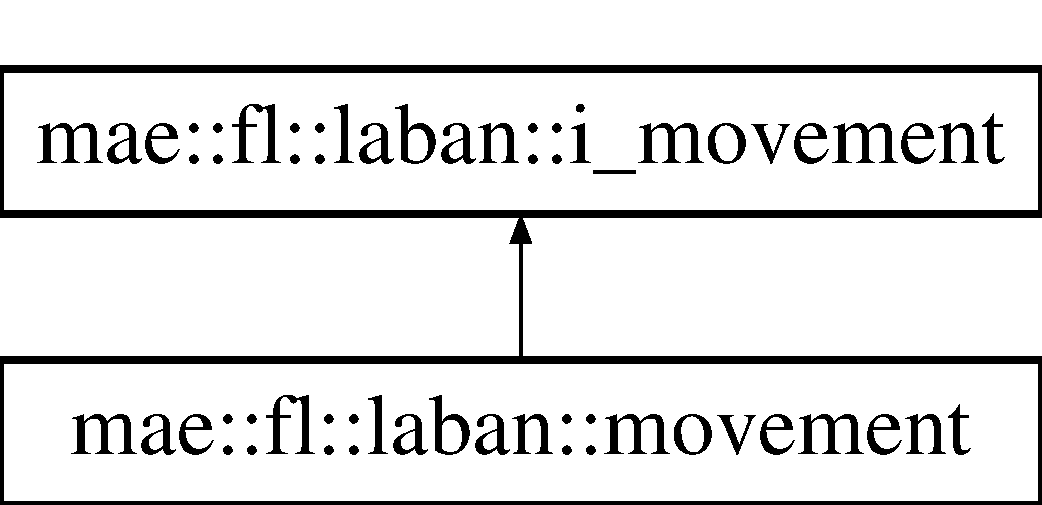
\includegraphics[height=2.000000cm]{classmae_1_1fl_1_1laban_1_1movement}
\end{center}
\end{figure}
\subsection*{Public Member Functions}
\begin{DoxyCompactItemize}
\item 
\hyperlink{classmae_1_1fl_1_1laban_1_1movement_a586715bc60b507e4b89b42dd54da8071}{movement} (int column, unsigned int measure, double beat, double duration, std\-::shared\-\_\-ptr$<$ \hyperlink{classmae_1_1fl_1_1laban_1_1mv_1_1i__symbol}{mv\-::i\-\_\-symbol} $>$ symbol, bool hold=false, std\-::shared\-\_\-ptr$<$ \hyperlink{classmae_1_1fl_1_1laban_1_1ps_1_1i__pre__sign}{ps\-::i\-\_\-pre\-\_\-sign} $>$ pre\-\_\-sign=nullptr)
\item 
virtual int \hyperlink{classmae_1_1fl_1_1laban_1_1movement_a7c6e91fd57b5cbec8d5d32901c9897d2}{get\-\_\-column} () const 
\item 
virtual unsigned int \hyperlink{classmae_1_1fl_1_1laban_1_1movement_a30bfe6e9dcfb8d6a26939285f2ff9583}{get\-\_\-measure} () const 
\item 
virtual double \hyperlink{classmae_1_1fl_1_1laban_1_1movement_a8dd1f022fc3402ece07a15863416d80a}{get\-\_\-beat} () const 
\item 
virtual double \hyperlink{classmae_1_1fl_1_1laban_1_1movement_aa1a2354ee3bc32fe218d53631d8c8d29}{get\-\_\-duration} () const 
\item 
std\-::shared\-\_\-ptr$<$ \hyperlink{classmae_1_1fl_1_1laban_1_1ps_1_1i__pre__sign}{ps\-::i\-\_\-pre\-\_\-sign} $>$ \hyperlink{classmae_1_1fl_1_1laban_1_1movement_af4de58bde35d683eaf1adc1d978d2a42}{get\-\_\-pre\-\_\-sign} () const 
\item 
bool \hyperlink{classmae_1_1fl_1_1laban_1_1movement_a51c69b15cef6525751bcd07f0e291688}{get\-\_\-hold} () const 
\item 
std\-::shared\-\_\-ptr$<$ \hyperlink{classmae_1_1fl_1_1laban_1_1mv_1_1i__symbol}{mv\-::i\-\_\-symbol} $>$ \hyperlink{classmae_1_1fl_1_1laban_1_1movement_ac6781745ae4c87fa0a5cfd1566619fee}{get\-\_\-symbol} () const 
\item 
virtual bool \hyperlink{classmae_1_1fl_1_1laban_1_1movement_a93b7f317d4ba358a641b43a21c09f228}{equals} (std\-::shared\-\_\-ptr$<$ \hyperlink{classmae_1_1fl_1_1laban_1_1i__movement}{i\-\_\-movement} $>$ a) const 
\item 
virtual bool \hyperlink{classmae_1_1fl_1_1laban_1_1movement_a6ddca6abc140bfd078473d1be23caf27}{symbol\-\_\-equals} (std\-::shared\-\_\-ptr$<$ \hyperlink{classmae_1_1fl_1_1laban_1_1i__movement}{i\-\_\-movement} $>$ a) const 
\item 
virtual std\-::string \hyperlink{classmae_1_1fl_1_1laban_1_1movement_abadb2cff01fb0835f042ce5a3b69300f}{xml} (unsigned int indent=0, std\-::string namesp=\char`\"{}\char`\"{}) const 
\item 
virtual std\-::string \hyperlink{classmae_1_1fl_1_1laban_1_1movement_a6ec35edce232832f663093f853a73d4c}{svg} (unsigned int im\-\_\-width, unsigned int im\-\_\-height, unsigned int max\-\_\-column, unsigned int measures, unsigned int beats\-\_\-per\-\_\-measure) const 
\item 
virtual std\-::shared\-\_\-ptr\\*
$<$ \hyperlink{classmae_1_1fl_1_1laban_1_1i__movement}{i\-\_\-movement} $>$ \hyperlink{classmae_1_1fl_1_1laban_1_1movement_af0c439b0b0d3c16516bce1953011922f}{recreate} (std\-::map$<$ int, int $>$ column\-\_\-mapping, unsigned int measure, double beat, double duration) const 
\item 
virtual std\-::string \hyperlink{classmae_1_1fl_1_1laban_1_1movement_a726883dc9180ead73f9039523367f1fc}{str} () const 
\end{DoxyCompactItemize}
\subsection*{Friends}
\begin{DoxyCompactItemize}
\item 
\hypertarget{classmae_1_1fl_1_1laban_1_1movement_af30ba5fdb954014180ce50b96cfb6797}{std\-::ostream \& {\bfseries operator$<$$<$} (std\-::ostream \&os, const \hyperlink{classmae_1_1fl_1_1laban_1_1movement}{movement} \&obj)}\label{classmae_1_1fl_1_1laban_1_1movement_af30ba5fdb954014180ce50b96cfb6797}

\item 
\hypertarget{classmae_1_1fl_1_1laban_1_1movement_a2239c926a5d434e8bb1e9bdf6a204224}{std\-::ostream \& {\bfseries operator$<$$<$} (std\-::ostream \&os, const std\-::shared\-\_\-ptr$<$ \hyperlink{classmae_1_1fl_1_1laban_1_1movement}{movement} $>$ \&obj)}\label{classmae_1_1fl_1_1laban_1_1movement_a2239c926a5d434e8bb1e9bdf6a204224}

\end{DoxyCompactItemize}


\subsection{Constructor \& Destructor Documentation}
\hypertarget{classmae_1_1fl_1_1laban_1_1movement_a586715bc60b507e4b89b42dd54da8071}{\index{mae\-::fl\-::laban\-::movement@{mae\-::fl\-::laban\-::movement}!movement@{movement}}
\index{movement@{movement}!mae::fl::laban::movement@{mae\-::fl\-::laban\-::movement}}
\subsubsection[{movement}]{\setlength{\rightskip}{0pt plus 5cm}mae\-::fl\-::laban\-::movement\-::movement (
\begin{DoxyParamCaption}
\item[{int}]{column, }
\item[{unsigned int}]{measure, }
\item[{double}]{beat, }
\item[{double}]{duration, }
\item[{std\-::shared\-\_\-ptr$<$ {\bf mv\-::i\-\_\-symbol} $>$}]{symbol, }
\item[{bool}]{hold = {\ttfamily false}, }
\item[{std\-::shared\-\_\-ptr$<$ {\bf ps\-::i\-\_\-pre\-\_\-sign} $>$}]{pre\-\_\-sign = {\ttfamily nullptr}}
\end{DoxyParamCaption}
)}}\label{classmae_1_1fl_1_1laban_1_1movement_a586715bc60b507e4b89b42dd54da8071}
Creates a movement element which represents a movement symbol in the score (e.\-g. direction and level or a turn) and (if present) a hold sign.


\begin{DoxyParams}{Parameters}
{\em column} & The column to which this symbol is meant to be added. \\
\hline
{\em measure} & The measure in which this symbol starts (and therefore the motion). \\
\hline
{\em beat} & The beat (decimals allowed) of the measure which is the beginning of the motion. \\
\hline
{\em duration} & The duration of the symbol (given in an amount of beats). \\
\hline
{\em symbol} & The symbol defining the kind of movement (e.\-g. direction+level or turn) \\
\hline
{\em hold} & If true a hold sign is attached to symbol. \\
\hline
{\em pre\-\_\-sign} & A pre-\/sign which can be used to address another body part than the one defined by the column. \\
\hline
\end{DoxyParams}


\subsection{Member Function Documentation}
\hypertarget{classmae_1_1fl_1_1laban_1_1movement_a93b7f317d4ba358a641b43a21c09f228}{\index{mae\-::fl\-::laban\-::movement@{mae\-::fl\-::laban\-::movement}!equals@{equals}}
\index{equals@{equals}!mae::fl::laban::movement@{mae\-::fl\-::laban\-::movement}}
\subsubsection[{equals}]{\setlength{\rightskip}{0pt plus 5cm}bool mae\-::fl\-::laban\-::movement\-::equals (
\begin{DoxyParamCaption}
\item[{std\-::shared\-\_\-ptr$<$ {\bf i\-\_\-movement} $>$}]{a}
\end{DoxyParamCaption}
) const\hspace{0.3cm}{\ttfamily [virtual]}}}\label{classmae_1_1fl_1_1laban_1_1movement_a93b7f317d4ba358a641b43a21c09f228}
Returns true if the \hyperlink{classmae_1_1fl_1_1laban_1_1i__movement}{i\-\_\-movement} elements are equal.


\begin{DoxyParams}{Parameters}
{\em a} & The movement to be compared to. \\
\hline
\end{DoxyParams}
\begin{DoxyReturn}{Returns}
True if equal. 
\end{DoxyReturn}


Implements \hyperlink{classmae_1_1fl_1_1laban_1_1i__movement_a29783771372283ff2cc7deded01b83b1}{mae\-::fl\-::laban\-::i\-\_\-movement}.

\hypertarget{classmae_1_1fl_1_1laban_1_1movement_a8dd1f022fc3402ece07a15863416d80a}{\index{mae\-::fl\-::laban\-::movement@{mae\-::fl\-::laban\-::movement}!get\-\_\-beat@{get\-\_\-beat}}
\index{get\-\_\-beat@{get\-\_\-beat}!mae::fl::laban::movement@{mae\-::fl\-::laban\-::movement}}
\subsubsection[{get\-\_\-beat}]{\setlength{\rightskip}{0pt plus 5cm}double mae\-::fl\-::laban\-::movement\-::get\-\_\-beat (
\begin{DoxyParamCaption}
{}
\end{DoxyParamCaption}
) const\hspace{0.3cm}{\ttfamily [virtual]}}}\label{classmae_1_1fl_1_1laban_1_1movement_a8dd1f022fc3402ece07a15863416d80a}
Returns the beat in which this symbol begins.

\begin{DoxyReturn}{Returns}

\end{DoxyReturn}


Implements \hyperlink{classmae_1_1fl_1_1laban_1_1i__movement_a2b8ee7b4d5cb5be09be93ff049fbdc68}{mae\-::fl\-::laban\-::i\-\_\-movement}.

\hypertarget{classmae_1_1fl_1_1laban_1_1movement_a7c6e91fd57b5cbec8d5d32901c9897d2}{\index{mae\-::fl\-::laban\-::movement@{mae\-::fl\-::laban\-::movement}!get\-\_\-column@{get\-\_\-column}}
\index{get\-\_\-column@{get\-\_\-column}!mae::fl::laban::movement@{mae\-::fl\-::laban\-::movement}}
\subsubsection[{get\-\_\-column}]{\setlength{\rightskip}{0pt plus 5cm}int mae\-::fl\-::laban\-::movement\-::get\-\_\-column (
\begin{DoxyParamCaption}
{}
\end{DoxyParamCaption}
) const\hspace{0.3cm}{\ttfamily [virtual]}}}\label{classmae_1_1fl_1_1laban_1_1movement_a7c6e91fd57b5cbec8d5d32901c9897d2}
Returns the column to which this symbol was added.

\begin{DoxyReturn}{Returns}

\end{DoxyReturn}


Implements \hyperlink{classmae_1_1fl_1_1laban_1_1i__movement_a448424f76457ed1dfa28e5d2c774c311}{mae\-::fl\-::laban\-::i\-\_\-movement}.

\hypertarget{classmae_1_1fl_1_1laban_1_1movement_aa1a2354ee3bc32fe218d53631d8c8d29}{\index{mae\-::fl\-::laban\-::movement@{mae\-::fl\-::laban\-::movement}!get\-\_\-duration@{get\-\_\-duration}}
\index{get\-\_\-duration@{get\-\_\-duration}!mae::fl::laban::movement@{mae\-::fl\-::laban\-::movement}}
\subsubsection[{get\-\_\-duration}]{\setlength{\rightskip}{0pt plus 5cm}double mae\-::fl\-::laban\-::movement\-::get\-\_\-duration (
\begin{DoxyParamCaption}
{}
\end{DoxyParamCaption}
) const\hspace{0.3cm}{\ttfamily [virtual]}}}\label{classmae_1_1fl_1_1laban_1_1movement_aa1a2354ee3bc32fe218d53631d8c8d29}
Returns the duration of the symbol.

\begin{DoxyReturn}{Returns}

\end{DoxyReturn}


Implements \hyperlink{classmae_1_1fl_1_1laban_1_1i__movement_ac83194ad9df8fed6c27199e83d35460d}{mae\-::fl\-::laban\-::i\-\_\-movement}.

\hypertarget{classmae_1_1fl_1_1laban_1_1movement_a51c69b15cef6525751bcd07f0e291688}{\index{mae\-::fl\-::laban\-::movement@{mae\-::fl\-::laban\-::movement}!get\-\_\-hold@{get\-\_\-hold}}
\index{get\-\_\-hold@{get\-\_\-hold}!mae::fl::laban::movement@{mae\-::fl\-::laban\-::movement}}
\subsubsection[{get\-\_\-hold}]{\setlength{\rightskip}{0pt plus 5cm}bool mae\-::fl\-::laban\-::movement\-::get\-\_\-hold (
\begin{DoxyParamCaption}
{}
\end{DoxyParamCaption}
) const}}\label{classmae_1_1fl_1_1laban_1_1movement_a51c69b15cef6525751bcd07f0e291688}
Returns true if a hold sign is attached.

\begin{DoxyReturn}{Returns}

\end{DoxyReturn}
\hypertarget{classmae_1_1fl_1_1laban_1_1movement_a30bfe6e9dcfb8d6a26939285f2ff9583}{\index{mae\-::fl\-::laban\-::movement@{mae\-::fl\-::laban\-::movement}!get\-\_\-measure@{get\-\_\-measure}}
\index{get\-\_\-measure@{get\-\_\-measure}!mae::fl::laban::movement@{mae\-::fl\-::laban\-::movement}}
\subsubsection[{get\-\_\-measure}]{\setlength{\rightskip}{0pt plus 5cm}unsigned int mae\-::fl\-::laban\-::movement\-::get\-\_\-measure (
\begin{DoxyParamCaption}
{}
\end{DoxyParamCaption}
) const\hspace{0.3cm}{\ttfamily [virtual]}}}\label{classmae_1_1fl_1_1laban_1_1movement_a30bfe6e9dcfb8d6a26939285f2ff9583}
Returns the measure in which this symbols begins. \begin{DoxyReturn}{Returns}

\end{DoxyReturn}


Implements \hyperlink{classmae_1_1fl_1_1laban_1_1i__movement_aa1b18a889adea3d1aa8a5a8af5de2de6}{mae\-::fl\-::laban\-::i\-\_\-movement}.

\hypertarget{classmae_1_1fl_1_1laban_1_1movement_af4de58bde35d683eaf1adc1d978d2a42}{\index{mae\-::fl\-::laban\-::movement@{mae\-::fl\-::laban\-::movement}!get\-\_\-pre\-\_\-sign@{get\-\_\-pre\-\_\-sign}}
\index{get\-\_\-pre\-\_\-sign@{get\-\_\-pre\-\_\-sign}!mae::fl::laban::movement@{mae\-::fl\-::laban\-::movement}}
\subsubsection[{get\-\_\-pre\-\_\-sign}]{\setlength{\rightskip}{0pt plus 5cm}std\-::shared\-\_\-ptr$<$ {\bf ps\-::i\-\_\-pre\-\_\-sign} $>$ mae\-::fl\-::laban\-::movement\-::get\-\_\-pre\-\_\-sign (
\begin{DoxyParamCaption}
{}
\end{DoxyParamCaption}
) const}}\label{classmae_1_1fl_1_1laban_1_1movement_af4de58bde35d683eaf1adc1d978d2a42}
Returns the pre sign if assigned. Returns null otherwise.

\begin{DoxyReturn}{Returns}

\end{DoxyReturn}
\hypertarget{classmae_1_1fl_1_1laban_1_1movement_ac6781745ae4c87fa0a5cfd1566619fee}{\index{mae\-::fl\-::laban\-::movement@{mae\-::fl\-::laban\-::movement}!get\-\_\-symbol@{get\-\_\-symbol}}
\index{get\-\_\-symbol@{get\-\_\-symbol}!mae::fl::laban::movement@{mae\-::fl\-::laban\-::movement}}
\subsubsection[{get\-\_\-symbol}]{\setlength{\rightskip}{0pt plus 5cm}std\-::shared\-\_\-ptr$<$ {\bf mv\-::i\-\_\-symbol} $>$ mae\-::fl\-::laban\-::movement\-::get\-\_\-symbol (
\begin{DoxyParamCaption}
{}
\end{DoxyParamCaption}
) const}}\label{classmae_1_1fl_1_1laban_1_1movement_ac6781745ae4c87fa0a5cfd1566619fee}
Returns the movement symbol.

\begin{DoxyReturn}{Returns}

\end{DoxyReturn}
\hypertarget{classmae_1_1fl_1_1laban_1_1movement_af0c439b0b0d3c16516bce1953011922f}{\index{mae\-::fl\-::laban\-::movement@{mae\-::fl\-::laban\-::movement}!recreate@{recreate}}
\index{recreate@{recreate}!mae::fl::laban::movement@{mae\-::fl\-::laban\-::movement}}
\subsubsection[{recreate}]{\setlength{\rightskip}{0pt plus 5cm}std\-::shared\-\_\-ptr$<$ {\bf i\-\_\-movement} $>$ mae\-::fl\-::laban\-::movement\-::recreate (
\begin{DoxyParamCaption}
\item[{std\-::map$<$ int, int $>$}]{column\-\_\-mapping, }
\item[{unsigned int}]{measure, }
\item[{double}]{beat, }
\item[{double}]{duration}
\end{DoxyParamCaption}
) const\hspace{0.3cm}{\ttfamily [virtual]}}}\label{classmae_1_1fl_1_1laban_1_1movement_af0c439b0b0d3c16516bce1953011922f}
Recreates the movement by copying its members but changing the position in the staff.


\begin{DoxyParams}{Parameters}
{\em column} & The new column. \\
\hline
{\em measure} & The new measure. \\
\hline
{\em beat} & The new beat. \\
\hline
{\em duration} & The new duration. \\
\hline
\end{DoxyParams}
\begin{DoxyReturn}{Returns}
The new, recreated movement. 
\end{DoxyReturn}


Implements \hyperlink{classmae_1_1fl_1_1laban_1_1i__movement_a28c8b00c68e291399281bda22e4f01f6}{mae\-::fl\-::laban\-::i\-\_\-movement}.

\hypertarget{classmae_1_1fl_1_1laban_1_1movement_a726883dc9180ead73f9039523367f1fc}{\index{mae\-::fl\-::laban\-::movement@{mae\-::fl\-::laban\-::movement}!str@{str}}
\index{str@{str}!mae::fl::laban::movement@{mae\-::fl\-::laban\-::movement}}
\subsubsection[{str}]{\setlength{\rightskip}{0pt plus 5cm}std\-::string mae\-::fl\-::laban\-::movement\-::str (
\begin{DoxyParamCaption}
{}
\end{DoxyParamCaption}
) const\hspace{0.3cm}{\ttfamily [virtual]}}}\label{classmae_1_1fl_1_1laban_1_1movement_a726883dc9180ead73f9039523367f1fc}
Returns the string representation for this element.

\begin{DoxyReturn}{Returns}
The string. 
\end{DoxyReturn}


Implements \hyperlink{classmae_1_1fl_1_1laban_1_1i__movement_a18322189d1851d3fd0f85c00b1051b57}{mae\-::fl\-::laban\-::i\-\_\-movement}.

\hypertarget{classmae_1_1fl_1_1laban_1_1movement_a6ec35edce232832f663093f853a73d4c}{\index{mae\-::fl\-::laban\-::movement@{mae\-::fl\-::laban\-::movement}!svg@{svg}}
\index{svg@{svg}!mae::fl::laban::movement@{mae\-::fl\-::laban\-::movement}}
\subsubsection[{svg}]{\setlength{\rightskip}{0pt plus 5cm}std\-::string mae\-::fl\-::laban\-::movement\-::svg (
\begin{DoxyParamCaption}
\item[{unsigned int}]{im\-\_\-width, }
\item[{unsigned int}]{im\-\_\-height, }
\item[{unsigned int}]{max\-\_\-column, }
\item[{unsigned int}]{measures, }
\item[{unsigned int}]{beats\-\_\-per\-\_\-measure}
\end{DoxyParamCaption}
) const\hspace{0.3cm}{\ttfamily [virtual]}}}\label{classmae_1_1fl_1_1laban_1_1movement_a6ec35edce232832f663093f853a73d4c}
Returns the S\-V\-G representation for this element.


\begin{DoxyParams}{Parameters}
{\em posx} & The x pos. \\
\hline
{\em posy} & The y pos. \\
\hline
{\em width} & The width. \\
\hline
{\em height} & The height. \\
\hline
\end{DoxyParams}
\begin{DoxyReturn}{Returns}
The S\-V\-G. 
\end{DoxyReturn}


Implements \hyperlink{classmae_1_1fl_1_1laban_1_1i__movement_ab2b0225ae8237b8ae410c797a0319498}{mae\-::fl\-::laban\-::i\-\_\-movement}.

\hypertarget{classmae_1_1fl_1_1laban_1_1movement_a6ddca6abc140bfd078473d1be23caf27}{\index{mae\-::fl\-::laban\-::movement@{mae\-::fl\-::laban\-::movement}!symbol\-\_\-equals@{symbol\-\_\-equals}}
\index{symbol\-\_\-equals@{symbol\-\_\-equals}!mae::fl::laban::movement@{mae\-::fl\-::laban\-::movement}}
\subsubsection[{symbol\-\_\-equals}]{\setlength{\rightskip}{0pt plus 5cm}bool mae\-::fl\-::laban\-::movement\-::symbol\-\_\-equals (
\begin{DoxyParamCaption}
\item[{std\-::shared\-\_\-ptr$<$ {\bf i\-\_\-movement} $>$}]{a}
\end{DoxyParamCaption}
) const\hspace{0.3cm}{\ttfamily [virtual]}}}\label{classmae_1_1fl_1_1laban_1_1movement_a6ddca6abc140bfd078473d1be23caf27}
Returns true if the symbols are equal. The position and duration are not regarded.


\begin{DoxyParams}{Parameters}
{\em a} & The movement to be compared to. \\
\hline
\end{DoxyParams}
\begin{DoxyReturn}{Returns}
True if symbols equal. 
\end{DoxyReturn}


Implements \hyperlink{classmae_1_1fl_1_1laban_1_1i__movement_a7b682911356dd13497172280b268ec40}{mae\-::fl\-::laban\-::i\-\_\-movement}.

\hypertarget{classmae_1_1fl_1_1laban_1_1movement_abadb2cff01fb0835f042ce5a3b69300f}{\index{mae\-::fl\-::laban\-::movement@{mae\-::fl\-::laban\-::movement}!xml@{xml}}
\index{xml@{xml}!mae::fl::laban::movement@{mae\-::fl\-::laban\-::movement}}
\subsubsection[{xml}]{\setlength{\rightskip}{0pt plus 5cm}std\-::string mae\-::fl\-::laban\-::movement\-::xml (
\begin{DoxyParamCaption}
\item[{unsigned int}]{indent = {\ttfamily 0}, }
\item[{std\-::string}]{namesp = {\ttfamily \char`\"{}\char`\"{}}}
\end{DoxyParamCaption}
) const\hspace{0.3cm}{\ttfamily [virtual]}}}\label{classmae_1_1fl_1_1laban_1_1movement_abadb2cff01fb0835f042ce5a3b69300f}
Returns the X\-M\-L representation for this element.


\begin{DoxyParams}{Parameters}
{\em indent} & The applied indent. \\
\hline
{\em namesp} & The prefixed X\-M\-L namespace.\\
\hline
\end{DoxyParams}
\begin{DoxyReturn}{Returns}
The X\-M\-L string. 
\end{DoxyReturn}


Implements \hyperlink{classmae_1_1fl_1_1laban_1_1i__movement_acd832b2a6976bfe32eae4bece01ee8f3}{mae\-::fl\-::laban\-::i\-\_\-movement}.



The documentation for this class was generated from the following files\-:\begin{DoxyCompactItemize}
\item 
src/mae/fl/laban/movement.\-hpp\item 
src/mae/fl/laban/movement.\-cpp\end{DoxyCompactItemize}

\hypertarget{classmae_1_1movement__controller}{\section{mae\-:\-:movement\-\_\-controller$<$ T, U $>$ Class Template Reference}
\label{classmae_1_1movement__controller}\index{mae\-::movement\-\_\-controller$<$ T, U $>$@{mae\-::movement\-\_\-controller$<$ T, U $>$}}
}
\subsection*{Public Member Functions}
\begin{DoxyCompactItemize}
\item 
\hyperlink{classmae_1_1movement__controller_a0a6d908fed45b190b0ce24faa879be47}{movement\-\_\-controller} (std\-::shared\-\_\-ptr$<$ \hyperlink{classmae_1_1i__movement__detector}{i\-\_\-movement\-\_\-detector}$<$ T, U $>$ $>$ imd, std\-::shared\-\_\-ptr$<$ \hyperlink{classmae_1_1i__sequence__recognizer}{i\-\_\-sequence\-\_\-recognizer}$<$ U $>$ $>$ isr, std\-::vector$<$ \hyperlink{classmae_1_1bone}{bone} $>$ body\-\_\-parts, int pose\-\_\-buffer\-\_\-size=0, double framerate=1.\-0/30.\-0, bool debug=false)
\item 
\hyperlink{classmae_1_1movement__controller_ac0ef0a57b48e4fb5f8c28168ea68f9e4}{movement\-\_\-controller} (std\-::shared\-\_\-ptr$<$ \hyperlink{classmae_1_1i__pose__detector}{i\-\_\-pose\-\_\-detector}$<$ T $>$ $>$ ipd, std\-::shared\-\_\-ptr$<$ \hyperlink{classmae_1_1i__sequence__generator}{i\-\_\-sequence\-\_\-generator}$<$ U $>$ $>$ isg, std\-::shared\-\_\-ptr$<$ \hyperlink{classmae_1_1i__sequence__recognizer}{i\-\_\-sequence\-\_\-recognizer}$<$ U $>$ $>$ isr, std\-::vector$<$ \hyperlink{classmae_1_1bone}{bone} $>$ body\-\_\-parts, int pose\-\_\-buffer\-\_\-size=0, double framerate=1.\-0/30.\-0, bool debug=false)
\item 
virtual void \hyperlink{classmae_1_1movement__controller_aa153304725199cb7d4664a0f450ec934}{next\-\_\-frame} (long timestamp, std\-::shared\-\_\-ptr$<$ T $>$ skeleton)
\item 
virtual void \hyperlink{classmae_1_1movement__controller_a67781bb43d01fcecfd4ab7c70c670bb9}{register\-\_\-sequence} (std\-::shared\-\_\-ptr$<$ U $>$ sequence)
\item 
virtual void \hyperlink{classmae_1_1movement__controller_a6b4bf0e71ad1c66fbea6cdae2913ef84}{deregister\-\_\-sequence} (std\-::shared\-\_\-ptr$<$ U $>$ sequence)
\item 
virtual void \hyperlink{classmae_1_1movement__controller_ac1fd2fc2b97bbc404e08f535647c47e9}{clear\-\_\-registered\-\_\-sequences} ()
\item 
virtual void \hyperlink{classmae_1_1movement__controller_a32f047751311a4e179d7cdad365bcadc}{set\-\_\-no\-\_\-buffer\-\_\-size\-\_\-update} (bool updates)
\item 
virtual void \hyperlink{classmae_1_1movement__controller_a6f99fd37e6d7459d311ba3cbcccbdea1}{set\-\_\-framerate} (double framerate)
\item 
virtual double \hyperlink{classmae_1_1movement__controller_af7f0769f77719733e2c73b9830d670fa}{get\-\_\-framerate} () const 
\item 
virtual void \hyperlink{classmae_1_1movement__controller_a694dc82c3222059711fa3a2ac6eb8ec2}{clear\-\_\-buffer} ()
\item 
virtual std\-::shared\-\_\-ptr$<$ U $>$ \hyperlink{classmae_1_1movement__controller_a8047034c7af70d1be6c63a33c8c7192c}{get\-\_\-current\-\_\-sequence} () const 
\item 
virtual std\-::shared\-\_\-ptr\\*
$<$ \hyperlink{classmae_1_1general__pose}{general\-\_\-pose} $>$ \hyperlink{classmae_1_1movement__controller_af6d4e2103bb880f25e43b93b6d83053a}{get\-\_\-current\-\_\-pose} () const 
\item 
virtual std\-::vector\\*
$<$ std\-::shared\-\_\-ptr$<$ U $>$ $>$ \hyperlink{classmae_1_1movement__controller_a58a04cf526d0deeffa7d4820619c41b5}{get\-\_\-current\-\_\-recognition} () const 
\item 
virtual void \hyperlink{classmae_1_1movement__controller_a7a150591c820312528d5b11e32646455}{add\-\_\-listener} (std\-::shared\-\_\-ptr$<$ \hyperlink{classmae_1_1i__pose__listener}{i\-\_\-pose\-\_\-listener} $>$ pose\-\_\-listener)
\item 
virtual void \hyperlink{classmae_1_1movement__controller_a5d77a42ac7427ae562d042ebbc6ce30b}{remove\-\_\-listener} (std\-::shared\-\_\-ptr$<$ \hyperlink{classmae_1_1i__pose__listener}{i\-\_\-pose\-\_\-listener} $>$ pose\-\_\-listener)
\item 
virtual void \hyperlink{classmae_1_1movement__controller_ade907e35d832e9ec5ec6fc2797df882f}{add\-\_\-listener} (std\-::shared\-\_\-ptr$<$ \hyperlink{classmae_1_1i__sequence__listener}{i\-\_\-sequence\-\_\-listener}$<$ U $>$ $>$ sequence\-\_\-listener)
\item 
virtual void \hyperlink{classmae_1_1movement__controller_af8e7fed43a0b64d09b7fbb22052ba635}{remove\-\_\-listener} (std\-::shared\-\_\-ptr$<$ \hyperlink{classmae_1_1i__sequence__listener}{i\-\_\-sequence\-\_\-listener}$<$ U $>$ $>$ sequence\-\_\-listener)
\item 
virtual void \hyperlink{classmae_1_1movement__controller_a80b292e1a12f916de2d167f22871c901}{add\-\_\-listener} (std\-::shared\-\_\-ptr$<$ \hyperlink{classmae_1_1i__recognition__listener}{i\-\_\-recognition\-\_\-listener}$<$ U $>$ $>$ recognition\-\_\-listener)
\item 
virtual void \hyperlink{classmae_1_1movement__controller_aafbffa6c9a0d2b73b2036f07c484b6cf}{remove\-\_\-listener} (std\-::shared\-\_\-ptr$<$ \hyperlink{classmae_1_1i__recognition__listener}{i\-\_\-recognition\-\_\-listener}$<$ U $>$ $>$ recognition\-\_\-listener)
\item 
virtual void \hyperlink{classmae_1_1movement__controller_adac2b632e8be6b8e2556005e79b187c3}{clear\-\_\-listeners} ()
\item 
virtual void \hyperlink{classmae_1_1movement__controller_a8e11558479a37a804102c94cfddde14d}{notify\-\_\-sequence\-\_\-listeners} (long timestamp, std\-::shared\-\_\-ptr$<$ U $>$ sequence)
\item 
virtual void \hyperlink{classmae_1_1movement__controller_a3b69de4b97cf639e621692ec8c8a9258}{notify\-\_\-recognition\-\_\-listeners} (long timestamp, std\-::vector$<$ std\-::shared\-\_\-ptr$<$ U $>$ $>$ sequences)
\item 
virtual std\-::shared\-\_\-ptr\\*
$<$ \hyperlink{classmae_1_1i__movement__detector}{i\-\_\-movement\-\_\-detector}$<$ T, U $>$ $>$ \hyperlink{classmae_1_1movement__controller_ad3d0a125556f02ce12a2ca7faf5c1cf3}{get\-\_\-movement\-\_\-detector} ()
\item 
virtual std\-::shared\-\_\-ptr\\*
$<$ \hyperlink{classmae_1_1i__sequence__recognizer}{i\-\_\-sequence\-\_\-recognizer}$<$ U $>$ $>$ \hyperlink{classmae_1_1movement__controller_af7d0eaa65d7a64e5b8169fef192760f6}{get\-\_\-sequence\-\_\-recognizer} ()
\end{DoxyCompactItemize}


\subsection{Constructor \& Destructor Documentation}
\hypertarget{classmae_1_1movement__controller_a0a6d908fed45b190b0ce24faa879be47}{\index{mae\-::movement\-\_\-controller@{mae\-::movement\-\_\-controller}!movement\-\_\-controller@{movement\-\_\-controller}}
\index{movement\-\_\-controller@{movement\-\_\-controller}!mae::movement_controller@{mae\-::movement\-\_\-controller}}
\subsubsection[{movement\-\_\-controller}]{\setlength{\rightskip}{0pt plus 5cm}template$<$typename T, typename U$>$ {\bf mae\-::movement\-\_\-controller}$<$ T, U $>$\-::{\bf movement\-\_\-controller} (
\begin{DoxyParamCaption}
\item[{std\-::shared\-\_\-ptr$<$ {\bf i\-\_\-movement\-\_\-detector}$<$ T, U $>$ $>$}]{imd, }
\item[{std\-::shared\-\_\-ptr$<$ {\bf i\-\_\-sequence\-\_\-recognizer}$<$ U $>$ $>$}]{isr, }
\item[{std\-::vector$<$ {\bf bone} $>$}]{body\-\_\-parts, }
\item[{int}]{pose\-\_\-buffer\-\_\-size = {\ttfamily 0}, }
\item[{double}]{framerate = {\ttfamily 1.0~/~30.0}, }
\item[{bool}]{debug = {\ttfamily false}}
\end{DoxyParamCaption}
)}}\label{classmae_1_1movement__controller_a0a6d908fed45b190b0ce24faa879be47}
Creates a new movement controller with controllers for the steps of the processing chain.


\begin{DoxyParams}{Parameters}
{\em imd} & The movement detector to detect sequences. \\
\hline
{\em isr} & The sequence recognizer to recognize sequences. \\
\hline
{\em body\-\_\-parts} & The addressed body parts. \\
\hline
{\em pose\-\_\-buffer\-\_\-size} & The initial pose buffer size. \\
\hline
{\em framerate} & The framerate of the skeleton stream. \\
\hline
{\em debug} & True for debug output on the terminal. \\
\hline
\end{DoxyParams}
\hypertarget{classmae_1_1movement__controller_ac0ef0a57b48e4fb5f8c28168ea68f9e4}{\index{mae\-::movement\-\_\-controller@{mae\-::movement\-\_\-controller}!movement\-\_\-controller@{movement\-\_\-controller}}
\index{movement\-\_\-controller@{movement\-\_\-controller}!mae::movement_controller@{mae\-::movement\-\_\-controller}}
\subsubsection[{movement\-\_\-controller}]{\setlength{\rightskip}{0pt plus 5cm}template$<$typename T, typename U$>$ {\bf mae\-::movement\-\_\-controller}$<$ T, U $>$\-::{\bf movement\-\_\-controller} (
\begin{DoxyParamCaption}
\item[{std\-::shared\-\_\-ptr$<$ {\bf i\-\_\-pose\-\_\-detector}$<$ T $>$ $>$}]{ipd, }
\item[{std\-::shared\-\_\-ptr$<$ {\bf i\-\_\-sequence\-\_\-generator}$<$ U $>$ $>$}]{isg, }
\item[{std\-::shared\-\_\-ptr$<$ {\bf i\-\_\-sequence\-\_\-recognizer}$<$ U $>$ $>$}]{isr, }
\item[{std\-::vector$<$ {\bf bone} $>$}]{body\-\_\-parts, }
\item[{int}]{pose\-\_\-buffer\-\_\-size = {\ttfamily 0}, }
\item[{double}]{framerate = {\ttfamily 1.0~/~30.0}, }
\item[{bool}]{debug = {\ttfamily false}}
\end{DoxyParamCaption}
)}}\label{classmae_1_1movement__controller_ac0ef0a57b48e4fb5f8c28168ea68f9e4}
Creates a new movement controller with controllers for the steps of the processing chain. The movement detector is built from the pose detector and the sequence generator. A key pose approach is used to do this.


\begin{DoxyParams}{Parameters}
{\em ipd} & The pose detector to detect poses from the stream. \\
\hline
{\em isg} & The sequence generator to generate sequences out of pose sequences. \\
\hline
{\em isr} & The sequence recognizer to recognize sequences. \\
\hline
{\em body\-\_\-parts} & The addressed body parts. \\
\hline
{\em pose\-\_\-buffer\-\_\-size} & The initial pose buffer size. \\
\hline
{\em framerate} & The framerate of the skeleton stream. \\
\hline
{\em debug} & True for debug output on the terminal. \\
\hline
\end{DoxyParams}


\subsection{Member Function Documentation}
\hypertarget{classmae_1_1movement__controller_a7a150591c820312528d5b11e32646455}{\index{mae\-::movement\-\_\-controller@{mae\-::movement\-\_\-controller}!add\-\_\-listener@{add\-\_\-listener}}
\index{add\-\_\-listener@{add\-\_\-listener}!mae::movement_controller@{mae\-::movement\-\_\-controller}}
\subsubsection[{add\-\_\-listener}]{\setlength{\rightskip}{0pt plus 5cm}template$<$typename T , typename U $>$ void {\bf mae\-::movement\-\_\-controller}$<$ T, U $>$\-::add\-\_\-listener (
\begin{DoxyParamCaption}
\item[{std\-::shared\-\_\-ptr$<$ {\bf i\-\_\-pose\-\_\-listener} $>$}]{pose\-\_\-listener}
\end{DoxyParamCaption}
)\hspace{0.3cm}{\ttfamily [virtual]}}}\label{classmae_1_1movement__controller_a7a150591c820312528d5b11e32646455}
Adds a pose listener to the movement controller. The pose listener is invoked whenever a pose was quantized (which is on every frame).


\begin{DoxyParams}{Parameters}
{\em pose\-\_\-listener} & The listener \\
\hline
\end{DoxyParams}
\hypertarget{classmae_1_1movement__controller_ade907e35d832e9ec5ec6fc2797df882f}{\index{mae\-::movement\-\_\-controller@{mae\-::movement\-\_\-controller}!add\-\_\-listener@{add\-\_\-listener}}
\index{add\-\_\-listener@{add\-\_\-listener}!mae::movement_controller@{mae\-::movement\-\_\-controller}}
\subsubsection[{add\-\_\-listener}]{\setlength{\rightskip}{0pt plus 5cm}template$<$typename T , typename U$>$ void {\bf mae\-::movement\-\_\-controller}$<$ T, U $>$\-::add\-\_\-listener (
\begin{DoxyParamCaption}
\item[{std\-::shared\-\_\-ptr$<$ {\bf i\-\_\-sequence\-\_\-listener}$<$ U $>$ $>$}]{sequence\-\_\-listener}
\end{DoxyParamCaption}
)\hspace{0.3cm}{\ttfamily [virtual]}}}\label{classmae_1_1movement__controller_ade907e35d832e9ec5ec6fc2797df882f}
Adds a sequence listener to the movement controller. The sequence listener is invoked whenever a sequence was generated (which is on every frame).


\begin{DoxyParams}{Parameters}
{\em sequence\-\_\-listener} & The listener \\
\hline
\end{DoxyParams}
\hypertarget{classmae_1_1movement__controller_a80b292e1a12f916de2d167f22871c901}{\index{mae\-::movement\-\_\-controller@{mae\-::movement\-\_\-controller}!add\-\_\-listener@{add\-\_\-listener}}
\index{add\-\_\-listener@{add\-\_\-listener}!mae::movement_controller@{mae\-::movement\-\_\-controller}}
\subsubsection[{add\-\_\-listener}]{\setlength{\rightskip}{0pt plus 5cm}template$<$typename T , typename U$>$ void {\bf mae\-::movement\-\_\-controller}$<$ T, U $>$\-::add\-\_\-listener (
\begin{DoxyParamCaption}
\item[{std\-::shared\-\_\-ptr$<$ {\bf i\-\_\-recognition\-\_\-listener}$<$ U $>$ $>$}]{recognition\-\_\-listener}
\end{DoxyParamCaption}
)\hspace{0.3cm}{\ttfamily [virtual]}}}\label{classmae_1_1movement__controller_a80b292e1a12f916de2d167f22871c901}
Adds a recognition listener to the controller. The recognition listener is invoked whenever a sequence was recognized.


\begin{DoxyParams}{Parameters}
{\em recognition\-\_\-listener} & The listener. \\
\hline
\end{DoxyParams}
\hypertarget{classmae_1_1movement__controller_a694dc82c3222059711fa3a2ac6eb8ec2}{\index{mae\-::movement\-\_\-controller@{mae\-::movement\-\_\-controller}!clear\-\_\-buffer@{clear\-\_\-buffer}}
\index{clear\-\_\-buffer@{clear\-\_\-buffer}!mae::movement_controller@{mae\-::movement\-\_\-controller}}
\subsubsection[{clear\-\_\-buffer}]{\setlength{\rightskip}{0pt plus 5cm}template$<$typename T , typename U $>$ void {\bf mae\-::movement\-\_\-controller}$<$ T, U $>$\-::clear\-\_\-buffer (
\begin{DoxyParamCaption}
{}
\end{DoxyParamCaption}
)\hspace{0.3cm}{\ttfamily [virtual]}}}\label{classmae_1_1movement__controller_a694dc82c3222059711fa3a2ac6eb8ec2}
Clears the buffer of currently present movements. \hypertarget{classmae_1_1movement__controller_adac2b632e8be6b8e2556005e79b187c3}{\index{mae\-::movement\-\_\-controller@{mae\-::movement\-\_\-controller}!clear\-\_\-listeners@{clear\-\_\-listeners}}
\index{clear\-\_\-listeners@{clear\-\_\-listeners}!mae::movement_controller@{mae\-::movement\-\_\-controller}}
\subsubsection[{clear\-\_\-listeners}]{\setlength{\rightskip}{0pt plus 5cm}template$<$typename T , typename U $>$ void {\bf mae\-::movement\-\_\-controller}$<$ T, U $>$\-::clear\-\_\-listeners (
\begin{DoxyParamCaption}
{}
\end{DoxyParamCaption}
)\hspace{0.3cm}{\ttfamily [virtual]}}}\label{classmae_1_1movement__controller_adac2b632e8be6b8e2556005e79b187c3}
Removes all listeners from the controller. \hypertarget{classmae_1_1movement__controller_ac1fd2fc2b97bbc404e08f535647c47e9}{\index{mae\-::movement\-\_\-controller@{mae\-::movement\-\_\-controller}!clear\-\_\-registered\-\_\-sequences@{clear\-\_\-registered\-\_\-sequences}}
\index{clear\-\_\-registered\-\_\-sequences@{clear\-\_\-registered\-\_\-sequences}!mae::movement_controller@{mae\-::movement\-\_\-controller}}
\subsubsection[{clear\-\_\-registered\-\_\-sequences}]{\setlength{\rightskip}{0pt plus 5cm}template$<$typename T , typename U $>$ void {\bf mae\-::movement\-\_\-controller}$<$ T, U $>$\-::clear\-\_\-registered\-\_\-sequences (
\begin{DoxyParamCaption}
{}
\end{DoxyParamCaption}
)\hspace{0.3cm}{\ttfamily [virtual]}}}\label{classmae_1_1movement__controller_ac1fd2fc2b97bbc404e08f535647c47e9}
Removes all registered sequences from the controller. \hypertarget{classmae_1_1movement__controller_a6b4bf0e71ad1c66fbea6cdae2913ef84}{\index{mae\-::movement\-\_\-controller@{mae\-::movement\-\_\-controller}!deregister\-\_\-sequence@{deregister\-\_\-sequence}}
\index{deregister\-\_\-sequence@{deregister\-\_\-sequence}!mae::movement_controller@{mae\-::movement\-\_\-controller}}
\subsubsection[{deregister\-\_\-sequence}]{\setlength{\rightskip}{0pt plus 5cm}template$<$typename T , typename U$>$ void {\bf mae\-::movement\-\_\-controller}$<$ T, U $>$\-::deregister\-\_\-sequence (
\begin{DoxyParamCaption}
\item[{std\-::shared\-\_\-ptr$<$ U $>$}]{sequence}
\end{DoxyParamCaption}
)\hspace{0.3cm}{\ttfamily [virtual]}}}\label{classmae_1_1movement__controller_a6b4bf0e71ad1c66fbea6cdae2913ef84}
Removes the registered sequence from the controller.


\begin{DoxyParams}{Parameters}
{\em sequence} & The sequence. \\
\hline
\end{DoxyParams}
\hypertarget{classmae_1_1movement__controller_af6d4e2103bb880f25e43b93b6d83053a}{\index{mae\-::movement\-\_\-controller@{mae\-::movement\-\_\-controller}!get\-\_\-current\-\_\-pose@{get\-\_\-current\-\_\-pose}}
\index{get\-\_\-current\-\_\-pose@{get\-\_\-current\-\_\-pose}!mae::movement_controller@{mae\-::movement\-\_\-controller}}
\subsubsection[{get\-\_\-current\-\_\-pose}]{\setlength{\rightskip}{0pt plus 5cm}template$<$typename T , typename U $>$ std\-::shared\-\_\-ptr$<$ {\bf general\-\_\-pose} $>$ {\bf mae\-::movement\-\_\-controller}$<$ T, U $>$\-::get\-\_\-current\-\_\-pose (
\begin{DoxyParamCaption}
{}
\end{DoxyParamCaption}
) const\hspace{0.3cm}{\ttfamily [virtual]}}}\label{classmae_1_1movement__controller_af6d4e2103bb880f25e43b93b6d83053a}
Returns the last processed pose.

\begin{DoxyReturn}{Returns}
The last processed pose. 
\end{DoxyReturn}
\hypertarget{classmae_1_1movement__controller_a58a04cf526d0deeffa7d4820619c41b5}{\index{mae\-::movement\-\_\-controller@{mae\-::movement\-\_\-controller}!get\-\_\-current\-\_\-recognition@{get\-\_\-current\-\_\-recognition}}
\index{get\-\_\-current\-\_\-recognition@{get\-\_\-current\-\_\-recognition}!mae::movement_controller@{mae\-::movement\-\_\-controller}}
\subsubsection[{get\-\_\-current\-\_\-recognition}]{\setlength{\rightskip}{0pt plus 5cm}template$<$typename T , typename U $>$ std\-::vector$<$ std\-::shared\-\_\-ptr$<$ U $>$ $>$ {\bf mae\-::movement\-\_\-controller}$<$ T, U $>$\-::get\-\_\-current\-\_\-recognition (
\begin{DoxyParamCaption}
{}
\end{DoxyParamCaption}
) const\hspace{0.3cm}{\ttfamily [virtual]}}}\label{classmae_1_1movement__controller_a58a04cf526d0deeffa7d4820619c41b5}
Returns the currently recognized sequences.

\begin{DoxyReturn}{Returns}
The sequences. 
\end{DoxyReturn}
\hypertarget{classmae_1_1movement__controller_a8047034c7af70d1be6c63a33c8c7192c}{\index{mae\-::movement\-\_\-controller@{mae\-::movement\-\_\-controller}!get\-\_\-current\-\_\-sequence@{get\-\_\-current\-\_\-sequence}}
\index{get\-\_\-current\-\_\-sequence@{get\-\_\-current\-\_\-sequence}!mae::movement_controller@{mae\-::movement\-\_\-controller}}
\subsubsection[{get\-\_\-current\-\_\-sequence}]{\setlength{\rightskip}{0pt plus 5cm}template$<$typename T , typename U $>$ std\-::shared\-\_\-ptr$<$ U $>$ {\bf mae\-::movement\-\_\-controller}$<$ T, U $>$\-::get\-\_\-current\-\_\-sequence (
\begin{DoxyParamCaption}
{}
\end{DoxyParamCaption}
) const\hspace{0.3cm}{\ttfamily [virtual]}}}\label{classmae_1_1movement__controller_a8047034c7af70d1be6c63a33c8c7192c}
Returns the currently generated sequence from the skeleton stream.

\begin{DoxyReturn}{Returns}
The sequence. 
\end{DoxyReturn}
\hypertarget{classmae_1_1movement__controller_af7f0769f77719733e2c73b9830d670fa}{\index{mae\-::movement\-\_\-controller@{mae\-::movement\-\_\-controller}!get\-\_\-framerate@{get\-\_\-framerate}}
\index{get\-\_\-framerate@{get\-\_\-framerate}!mae::movement_controller@{mae\-::movement\-\_\-controller}}
\subsubsection[{get\-\_\-framerate}]{\setlength{\rightskip}{0pt plus 5cm}template$<$typename T , typename U $>$ double {\bf mae\-::movement\-\_\-controller}$<$ T, U $>$\-::get\-\_\-framerate (
\begin{DoxyParamCaption}
{}
\end{DoxyParamCaption}
) const\hspace{0.3cm}{\ttfamily [virtual]}}}\label{classmae_1_1movement__controller_af7f0769f77719733e2c73b9830d670fa}
Returns the currently applied framerate.

\begin{DoxyReturn}{Returns}
The framerate. 
\end{DoxyReturn}
\hypertarget{classmae_1_1movement__controller_ad3d0a125556f02ce12a2ca7faf5c1cf3}{\index{mae\-::movement\-\_\-controller@{mae\-::movement\-\_\-controller}!get\-\_\-movement\-\_\-detector@{get\-\_\-movement\-\_\-detector}}
\index{get\-\_\-movement\-\_\-detector@{get\-\_\-movement\-\_\-detector}!mae::movement_controller@{mae\-::movement\-\_\-controller}}
\subsubsection[{get\-\_\-movement\-\_\-detector}]{\setlength{\rightskip}{0pt plus 5cm}template$<$typename T , typename U $>$ std\-::shared\-\_\-ptr$<$ {\bf i\-\_\-movement\-\_\-detector}$<$ T, U $>$ $>$ {\bf mae\-::movement\-\_\-controller}$<$ T, U $>$\-::get\-\_\-movement\-\_\-detector (
\begin{DoxyParamCaption}
{}
\end{DoxyParamCaption}
)\hspace{0.3cm}{\ttfamily [virtual]}}}\label{classmae_1_1movement__controller_ad3d0a125556f02ce12a2ca7faf5c1cf3}
Returns the movement detector which is registered to this controller.

\begin{DoxyReturn}{Returns}
The movement detector. 
\end{DoxyReturn}
\hypertarget{classmae_1_1movement__controller_af7d0eaa65d7a64e5b8169fef192760f6}{\index{mae\-::movement\-\_\-controller@{mae\-::movement\-\_\-controller}!get\-\_\-sequence\-\_\-recognizer@{get\-\_\-sequence\-\_\-recognizer}}
\index{get\-\_\-sequence\-\_\-recognizer@{get\-\_\-sequence\-\_\-recognizer}!mae::movement_controller@{mae\-::movement\-\_\-controller}}
\subsubsection[{get\-\_\-sequence\-\_\-recognizer}]{\setlength{\rightskip}{0pt plus 5cm}template$<$typename T , typename U $>$ std\-::shared\-\_\-ptr$<$ {\bf i\-\_\-sequence\-\_\-recognizer}$<$ U $>$ $>$ {\bf mae\-::movement\-\_\-controller}$<$ T, U $>$\-::get\-\_\-sequence\-\_\-recognizer (
\begin{DoxyParamCaption}
{}
\end{DoxyParamCaption}
)\hspace{0.3cm}{\ttfamily [virtual]}}}\label{classmae_1_1movement__controller_af7d0eaa65d7a64e5b8169fef192760f6}
Returns the sequence recognizer which is registered to this controller.

\begin{DoxyReturn}{Returns}
The sequence recognizer. 
\end{DoxyReturn}
\hypertarget{classmae_1_1movement__controller_aa153304725199cb7d4664a0f450ec934}{\index{mae\-::movement\-\_\-controller@{mae\-::movement\-\_\-controller}!next\-\_\-frame@{next\-\_\-frame}}
\index{next\-\_\-frame@{next\-\_\-frame}!mae::movement_controller@{mae\-::movement\-\_\-controller}}
\subsubsection[{next\-\_\-frame}]{\setlength{\rightskip}{0pt plus 5cm}template$<$typename T, typename U $>$ void {\bf mae\-::movement\-\_\-controller}$<$ T, U $>$\-::next\-\_\-frame (
\begin{DoxyParamCaption}
\item[{long}]{timestamp, }
\item[{std\-::shared\-\_\-ptr$<$ T $>$}]{skeleton}
\end{DoxyParamCaption}
)\hspace{0.3cm}{\ttfamily [virtual]}}}\label{classmae_1_1movement__controller_aa153304725199cb7d4664a0f450ec934}
Processes the next frame.


\begin{DoxyParams}{Parameters}
{\em timestamp} & The timestamp for the skeleton. \\
\hline
{\em skeleton} & The skeleton. \\
\hline
\end{DoxyParams}
\hypertarget{classmae_1_1movement__controller_a3b69de4b97cf639e621692ec8c8a9258}{\index{mae\-::movement\-\_\-controller@{mae\-::movement\-\_\-controller}!notify\-\_\-recognition\-\_\-listeners@{notify\-\_\-recognition\-\_\-listeners}}
\index{notify\-\_\-recognition\-\_\-listeners@{notify\-\_\-recognition\-\_\-listeners}!mae::movement_controller@{mae\-::movement\-\_\-controller}}
\subsubsection[{notify\-\_\-recognition\-\_\-listeners}]{\setlength{\rightskip}{0pt plus 5cm}template$<$typename T , typename U$>$ void {\bf mae\-::movement\-\_\-controller}$<$ T, U $>$\-::notify\-\_\-recognition\-\_\-listeners (
\begin{DoxyParamCaption}
\item[{long}]{timestamp, }
\item[{std\-::vector$<$ std\-::shared\-\_\-ptr$<$ U $>$ $>$}]{sequences}
\end{DoxyParamCaption}
)\hspace{0.3cm}{\ttfamily [virtual]}}}\label{classmae_1_1movement__controller_a3b69de4b97cf639e621692ec8c8a9258}
Notifies the recognition listeners on recognized sequences.


\begin{DoxyParams}{Parameters}
{\em timestamp} & The timestamp. \\
\hline
{\em sequences} & The recognized sequences. \\
\hline
\end{DoxyParams}
\hypertarget{classmae_1_1movement__controller_a8e11558479a37a804102c94cfddde14d}{\index{mae\-::movement\-\_\-controller@{mae\-::movement\-\_\-controller}!notify\-\_\-sequence\-\_\-listeners@{notify\-\_\-sequence\-\_\-listeners}}
\index{notify\-\_\-sequence\-\_\-listeners@{notify\-\_\-sequence\-\_\-listeners}!mae::movement_controller@{mae\-::movement\-\_\-controller}}
\subsubsection[{notify\-\_\-sequence\-\_\-listeners}]{\setlength{\rightskip}{0pt plus 5cm}template$<$typename T , typename U$>$ void {\bf mae\-::movement\-\_\-controller}$<$ T, U $>$\-::notify\-\_\-sequence\-\_\-listeners (
\begin{DoxyParamCaption}
\item[{long}]{timestamp, }
\item[{std\-::shared\-\_\-ptr$<$ U $>$}]{sequence}
\end{DoxyParamCaption}
)\hspace{0.3cm}{\ttfamily [virtual]}}}\label{classmae_1_1movement__controller_a8e11558479a37a804102c94cfddde14d}
Notifies the sequence listeners on a newly generated sequence.


\begin{DoxyParams}{Parameters}
{\em timestamp} & The timestamp. \\
\hline
{\em sequence} & The sequence. \\
\hline
\end{DoxyParams}
\hypertarget{classmae_1_1movement__controller_a67781bb43d01fcecfd4ab7c70c670bb9}{\index{mae\-::movement\-\_\-controller@{mae\-::movement\-\_\-controller}!register\-\_\-sequence@{register\-\_\-sequence}}
\index{register\-\_\-sequence@{register\-\_\-sequence}!mae::movement_controller@{mae\-::movement\-\_\-controller}}
\subsubsection[{register\-\_\-sequence}]{\setlength{\rightskip}{0pt plus 5cm}template$<$typename T , typename U$>$ void {\bf mae\-::movement\-\_\-controller}$<$ T, U $>$\-::register\-\_\-sequence (
\begin{DoxyParamCaption}
\item[{std\-::shared\-\_\-ptr$<$ U $>$}]{sequence}
\end{DoxyParamCaption}
)\hspace{0.3cm}{\ttfamily [virtual]}}}\label{classmae_1_1movement__controller_a67781bb43d01fcecfd4ab7c70c670bb9}
Registers a sequence to the controller in order to be recognized from the stream.


\begin{DoxyParams}{Parameters}
{\em sequence} & The sequence. \\
\hline
\end{DoxyParams}
\hypertarget{classmae_1_1movement__controller_a5d77a42ac7427ae562d042ebbc6ce30b}{\index{mae\-::movement\-\_\-controller@{mae\-::movement\-\_\-controller}!remove\-\_\-listener@{remove\-\_\-listener}}
\index{remove\-\_\-listener@{remove\-\_\-listener}!mae::movement_controller@{mae\-::movement\-\_\-controller}}
\subsubsection[{remove\-\_\-listener}]{\setlength{\rightskip}{0pt plus 5cm}template$<$typename T , typename U $>$ void {\bf mae\-::movement\-\_\-controller}$<$ T, U $>$\-::remove\-\_\-listener (
\begin{DoxyParamCaption}
\item[{std\-::shared\-\_\-ptr$<$ {\bf i\-\_\-pose\-\_\-listener} $>$}]{pose\-\_\-listener}
\end{DoxyParamCaption}
)\hspace{0.3cm}{\ttfamily [virtual]}}}\label{classmae_1_1movement__controller_a5d77a42ac7427ae562d042ebbc6ce30b}
Removes the pose listener from the controller.


\begin{DoxyParams}{Parameters}
{\em pose\-\_\-listener} & The listener. \\
\hline
\end{DoxyParams}
\hypertarget{classmae_1_1movement__controller_af8e7fed43a0b64d09b7fbb22052ba635}{\index{mae\-::movement\-\_\-controller@{mae\-::movement\-\_\-controller}!remove\-\_\-listener@{remove\-\_\-listener}}
\index{remove\-\_\-listener@{remove\-\_\-listener}!mae::movement_controller@{mae\-::movement\-\_\-controller}}
\subsubsection[{remove\-\_\-listener}]{\setlength{\rightskip}{0pt plus 5cm}template$<$typename T , typename U$>$ void {\bf mae\-::movement\-\_\-controller}$<$ T, U $>$\-::remove\-\_\-listener (
\begin{DoxyParamCaption}
\item[{std\-::shared\-\_\-ptr$<$ {\bf i\-\_\-sequence\-\_\-listener}$<$ U $>$ $>$}]{sequence\-\_\-listener}
\end{DoxyParamCaption}
)\hspace{0.3cm}{\ttfamily [virtual]}}}\label{classmae_1_1movement__controller_af8e7fed43a0b64d09b7fbb22052ba635}
Removes the sequence listener from the controller.


\begin{DoxyParams}{Parameters}
{\em sequence\-\_\-listener} & The listener \\
\hline
\end{DoxyParams}
\hypertarget{classmae_1_1movement__controller_aafbffa6c9a0d2b73b2036f07c484b6cf}{\index{mae\-::movement\-\_\-controller@{mae\-::movement\-\_\-controller}!remove\-\_\-listener@{remove\-\_\-listener}}
\index{remove\-\_\-listener@{remove\-\_\-listener}!mae::movement_controller@{mae\-::movement\-\_\-controller}}
\subsubsection[{remove\-\_\-listener}]{\setlength{\rightskip}{0pt plus 5cm}template$<$typename T , typename U$>$ void {\bf mae\-::movement\-\_\-controller}$<$ T, U $>$\-::remove\-\_\-listener (
\begin{DoxyParamCaption}
\item[{std\-::shared\-\_\-ptr$<$ {\bf i\-\_\-recognition\-\_\-listener}$<$ U $>$ $>$}]{recognition\-\_\-listener}
\end{DoxyParamCaption}
)\hspace{0.3cm}{\ttfamily [virtual]}}}\label{classmae_1_1movement__controller_aafbffa6c9a0d2b73b2036f07c484b6cf}
Removes the recognition listener from the controller.


\begin{DoxyParams}{Parameters}
{\em sequence\-\_\-listener} & The listener \\
\hline
\end{DoxyParams}
\hypertarget{classmae_1_1movement__controller_a6f99fd37e6d7459d311ba3cbcccbdea1}{\index{mae\-::movement\-\_\-controller@{mae\-::movement\-\_\-controller}!set\-\_\-framerate@{set\-\_\-framerate}}
\index{set\-\_\-framerate@{set\-\_\-framerate}!mae::movement_controller@{mae\-::movement\-\_\-controller}}
\subsubsection[{set\-\_\-framerate}]{\setlength{\rightskip}{0pt plus 5cm}template$<$typename T , typename U $>$ void {\bf mae\-::movement\-\_\-controller}$<$ T, U $>$\-::set\-\_\-framerate (
\begin{DoxyParamCaption}
\item[{double}]{framerate}
\end{DoxyParamCaption}
)\hspace{0.3cm}{\ttfamily [virtual]}}}\label{classmae_1_1movement__controller_a6f99fd37e6d7459d311ba3cbcccbdea1}
Sets the framerate to be applied.


\begin{DoxyParams}{Parameters}
{\em framerate} & The framerate \\
\hline
\end{DoxyParams}
\hypertarget{classmae_1_1movement__controller_a32f047751311a4e179d7cdad365bcadc}{\index{mae\-::movement\-\_\-controller@{mae\-::movement\-\_\-controller}!set\-\_\-no\-\_\-buffer\-\_\-size\-\_\-update@{set\-\_\-no\-\_\-buffer\-\_\-size\-\_\-update}}
\index{set\-\_\-no\-\_\-buffer\-\_\-size\-\_\-update@{set\-\_\-no\-\_\-buffer\-\_\-size\-\_\-update}!mae::movement_controller@{mae\-::movement\-\_\-controller}}
\subsubsection[{set\-\_\-no\-\_\-buffer\-\_\-size\-\_\-update}]{\setlength{\rightskip}{0pt plus 5cm}template$<$typename T , typename U $>$ void {\bf mae\-::movement\-\_\-controller}$<$ T, U $>$\-::set\-\_\-no\-\_\-buffer\-\_\-size\-\_\-update (
\begin{DoxyParamCaption}
\item[{bool}]{updates}
\end{DoxyParamCaption}
)\hspace{0.3cm}{\ttfamily [virtual]}}}\label{classmae_1_1movement__controller_a32f047751311a4e179d7cdad365bcadc}
Disables or enables buffer size updates on newly registered sequences.


\begin{DoxyParams}{Parameters}
{\em updates} & True for automatic updates of the buffer size. \\
\hline
\end{DoxyParams}


The documentation for this class was generated from the following file\-:\begin{DoxyCompactItemize}
\item 
src/mae/movement\-\_\-controller.\-hpp\end{DoxyCompactItemize}

\hypertarget{classmae_1_1mstr}{\section{mae\-:\-:mstr Class Reference}
\label{classmae_1_1mstr}\index{mae\-::mstr@{mae\-::mstr}}
}
\subsection*{Static Public Member Functions}
\begin{DoxyCompactItemize}
\item 
static std\-::string \hyperlink{classmae_1_1mstr_a56bbcec6911fdb586e467c0910705e2d}{trim\-\_\-left} (const std\-::string \&value)
\item 
static std\-::string \hyperlink{classmae_1_1mstr_abf762858f021f667c97818eb7fe23837}{trim\-\_\-right} (const std\-::string \&value)
\item 
static std\-::string \hyperlink{classmae_1_1mstr_abb7fe37e72163a15dc8421cc196d53b6}{trim} (const std\-::string \&value)
\item 
static void \hyperlink{classmae_1_1mstr_ab6a08ae2af015c92d84168c85214b9c5}{trim\-\_\-quotes} (std\-::string $\ast$value)
\item 
static std\-::string \hyperlink{classmae_1_1mstr_a194034daef724a50a5e97a7c9a9e0ff6}{replace} (const std\-::string \&haystack, const std\-::string \&needle, const std\-::string \&replacement)
\item 
static std\-::string \hyperlink{classmae_1_1mstr_a0cbe11fc882f95e92bdfeb74dd124de5}{replace\-\_\-esc} (const std\-::string \&haystack, const std\-::string \&needle, const std\-::string \&replacement)
\item 
static std\-::string \hyperlink{classmae_1_1mstr_a44ff1149a740f19fba40d20c15a75c24}{replace\-\_\-unesc} (const std\-::string \&haystack, const std\-::string \&needle, const std\-::string \&replacement)
\item 
static std\-::string \hyperlink{classmae_1_1mstr_a6406c61f815538d381b8c403753780d2}{to\-\_\-lower} (const std\-::string \&value)
\item 
static std\-::string \hyperlink{classmae_1_1mstr_a59d49fd43569aecdbdaf8370439c6527}{to\-\_\-upper} (const std\-::string \&value)
\item 
static std\-::pair\\*
$<$ std\-::string\-::size\-\_\-type, \\*
std\-::string\-::size\-\_\-type $>$ \hyperlink{classmae_1_1mstr_a73b0a7ad10467d7b2ed2ca496ce3b031}{find\-\_\-line} (const std\-::string \&haystack, const std\-::string \&needle)
\item 
static std\-::pair\\*
$<$ std\-::string\-::size\-\_\-type, \\*
std\-::string\-::size\-\_\-type $>$ \hyperlink{classmae_1_1mstr_ab8d16fb69051273d679b1c6c0ab74176}{find\-\_\-line} (const std\-::string \&haystack, const std\-::string \&needle, std\-::string\-::size\-\_\-type pos)
\item 
static std\-::vector$<$ std\-::string $>$ \hyperlink{classmae_1_1mstr_a6806a6a419a45340529ce00477054862}{split} (const std\-::string \&value)
\item 
static std\-::vector$<$ std\-::string $>$ \hyperlink{classmae_1_1mstr_a4359ed2982005150b97cdd7f517643c4}{split} (const std\-::string \&value, std\-::string\-::size\-\_\-type pos, std\-::string\-::size\-\_\-type n)
\item 
static std\-::vector$<$ std\-::string $>$ \hyperlink{classmae_1_1mstr_ab630b766d528f6841d3f559a323c54fd}{split} (const std\-::string \&value, char delim)
\item 
static std\-::vector$<$ std\-::string $>$ \hyperlink{classmae_1_1mstr_a0f8941949474f4f5ad9c3e254e673275}{split} (const std\-::string \&value, char delim, std\-::string\-::size\-\_\-type pos, std\-::string\-::size\-\_\-type n)
\item 
static std\-::vector$<$ double $>$ \hyperlink{classmae_1_1mstr_a28c61cea982e00cb4829ce679e86701e}{double\-\_\-list} (const std\-::string \&value)
\item 
static std\-::vector$<$ double $>$ \hyperlink{classmae_1_1mstr_a242484e54378dc9ace617609fdf86b15}{double\-\_\-list} (const std\-::string \&value, std\-::string\-::size\-\_\-type pos, std\-::string\-::size\-\_\-type n)
\end{DoxyCompactItemize}


\subsection{Member Function Documentation}
\hypertarget{classmae_1_1mstr_a28c61cea982e00cb4829ce679e86701e}{\index{mae\-::mstr@{mae\-::mstr}!double\-\_\-list@{double\-\_\-list}}
\index{double\-\_\-list@{double\-\_\-list}!mae::mstr@{mae\-::mstr}}
\subsubsection[{double\-\_\-list}]{\setlength{\rightskip}{0pt plus 5cm}std\-::vector$<$ double $>$ mae\-::mstr\-::double\-\_\-list (
\begin{DoxyParamCaption}
\item[{const std\-::string \&}]{value}
\end{DoxyParamCaption}
)\hspace{0.3cm}{\ttfamily [static]}}}\label{classmae_1_1mstr_a28c61cea982e00cb4829ce679e86701e}
Splits the string and parses the values to doubles.


\begin{DoxyParams}{Parameters}
{\em value} & The string. \\
\hline
\end{DoxyParams}
\begin{DoxyReturn}{Returns}
The result. 
\end{DoxyReturn}
\hypertarget{classmae_1_1mstr_a242484e54378dc9ace617609fdf86b15}{\index{mae\-::mstr@{mae\-::mstr}!double\-\_\-list@{double\-\_\-list}}
\index{double\-\_\-list@{double\-\_\-list}!mae::mstr@{mae\-::mstr}}
\subsubsection[{double\-\_\-list}]{\setlength{\rightskip}{0pt plus 5cm}std\-::vector$<$ double $>$ mae\-::mstr\-::double\-\_\-list (
\begin{DoxyParamCaption}
\item[{const std\-::string \&}]{value, }
\item[{std\-::string\-::size\-\_\-type}]{pos, }
\item[{std\-::string\-::size\-\_\-type}]{n}
\end{DoxyParamCaption}
)\hspace{0.3cm}{\ttfamily [static]}}}\label{classmae_1_1mstr_a242484e54378dc9ace617609fdf86b15}
Splits the string and parses the values to doubles beginning at the given position and regarding only n characters.


\begin{DoxyParams}{Parameters}
{\em value} & The string. \\
\hline
{\em pos} & The start position for the split. \\
\hline
{\em n} & The number of characters to be regarded. \\
\hline
\end{DoxyParams}
\begin{DoxyReturn}{Returns}
The result. 
\end{DoxyReturn}
\hypertarget{classmae_1_1mstr_a73b0a7ad10467d7b2ed2ca496ce3b031}{\index{mae\-::mstr@{mae\-::mstr}!find\-\_\-line@{find\-\_\-line}}
\index{find\-\_\-line@{find\-\_\-line}!mae::mstr@{mae\-::mstr}}
\subsubsection[{find\-\_\-line}]{\setlength{\rightskip}{0pt plus 5cm}std\-::pair$<$ std\-::string\-::size\-\_\-type, std\-::string\-::size\-\_\-type $>$ mae\-::mstr\-::find\-\_\-line (
\begin{DoxyParamCaption}
\item[{const std\-::string \&}]{haystack, }
\item[{const std\-::string \&}]{needle}
\end{DoxyParamCaption}
)\hspace{0.3cm}{\ttfamily [static]}}}\label{classmae_1_1mstr_a73b0a7ad10467d7b2ed2ca496ce3b031}
Find the first occurence of the needle in the line and returns the line break too.


\begin{DoxyParams}{Parameters}
{\em haystack} & The haystack. \\
\hline
{\em needle} & The needle. \\
\hline
\end{DoxyParams}
\begin{DoxyReturn}{Returns}
A pair of positions defining the occurence of the needle and the end of line. 
\end{DoxyReturn}
\hypertarget{classmae_1_1mstr_ab8d16fb69051273d679b1c6c0ab74176}{\index{mae\-::mstr@{mae\-::mstr}!find\-\_\-line@{find\-\_\-line}}
\index{find\-\_\-line@{find\-\_\-line}!mae::mstr@{mae\-::mstr}}
\subsubsection[{find\-\_\-line}]{\setlength{\rightskip}{0pt plus 5cm}std\-::pair$<$ std\-::string\-::size\-\_\-type, std\-::string\-::size\-\_\-type $>$ mae\-::mstr\-::find\-\_\-line (
\begin{DoxyParamCaption}
\item[{const std\-::string \&}]{haystack, }
\item[{const std\-::string \&}]{needle, }
\item[{std\-::string\-::size\-\_\-type}]{pos}
\end{DoxyParamCaption}
)\hspace{0.3cm}{\ttfamily [static]}}}\label{classmae_1_1mstr_ab8d16fb69051273d679b1c6c0ab74176}
Find the first occurence of the needle after the given position in the line and returns the line break too.


\begin{DoxyParams}{Parameters}
{\em haystack} & The haystack. \\
\hline
{\em needle} & The needle. \\
\hline
{\em pos} & The start position of the search. \\
\hline
\end{DoxyParams}
\begin{DoxyReturn}{Returns}
A pair of positions defining the occurence of the needle and the end of line. 
\end{DoxyReturn}
\hypertarget{classmae_1_1mstr_a194034daef724a50a5e97a7c9a9e0ff6}{\index{mae\-::mstr@{mae\-::mstr}!replace@{replace}}
\index{replace@{replace}!mae::mstr@{mae\-::mstr}}
\subsubsection[{replace}]{\setlength{\rightskip}{0pt plus 5cm}std\-::string mae\-::mstr\-::replace (
\begin{DoxyParamCaption}
\item[{const std\-::string \&}]{haystack, }
\item[{const std\-::string \&}]{needle, }
\item[{const std\-::string \&}]{replacement}
\end{DoxyParamCaption}
)\hspace{0.3cm}{\ttfamily [static]}}}\label{classmae_1_1mstr_a194034daef724a50a5e97a7c9a9e0ff6}
Replaces all occurences in the haystack with the given replacement.


\begin{DoxyParams}{Parameters}
{\em haystack} & The haystack. \\
\hline
{\em needle} & The needle. \\
\hline
{\em replacement} & The replacement. \\
\hline
\end{DoxyParams}
\begin{DoxyReturn}{Returns}
The result. 
\end{DoxyReturn}
\hypertarget{classmae_1_1mstr_a0cbe11fc882f95e92bdfeb74dd124de5}{\index{mae\-::mstr@{mae\-::mstr}!replace\-\_\-esc@{replace\-\_\-esc}}
\index{replace\-\_\-esc@{replace\-\_\-esc}!mae::mstr@{mae\-::mstr}}
\subsubsection[{replace\-\_\-esc}]{\setlength{\rightskip}{0pt plus 5cm}std\-::string mae\-::mstr\-::replace\-\_\-esc (
\begin{DoxyParamCaption}
\item[{const std\-::string \&}]{haystack, }
\item[{const std\-::string \&}]{needle, }
\item[{const std\-::string \&}]{replacement}
\end{DoxyParamCaption}
)\hspace{0.3cm}{\ttfamily [static]}}}\label{classmae_1_1mstr_a0cbe11fc882f95e92bdfeb74dd124de5}
Replaces all occurrences in the haystack with the given replacement. Escapes all occurrences of the replacement with '\textbackslash{}'.


\begin{DoxyParams}{Parameters}
{\em haystack} & The haystack. \\
\hline
{\em needle} & The needle. \\
\hline
{\em replacement} & The replacement. \\
\hline
\end{DoxyParams}
\begin{DoxyReturn}{Returns}
The result. 

The result. 
\end{DoxyReturn}
\hypertarget{classmae_1_1mstr_a44ff1149a740f19fba40d20c15a75c24}{\index{mae\-::mstr@{mae\-::mstr}!replace\-\_\-unesc@{replace\-\_\-unesc}}
\index{replace\-\_\-unesc@{replace\-\_\-unesc}!mae::mstr@{mae\-::mstr}}
\subsubsection[{replace\-\_\-unesc}]{\setlength{\rightskip}{0pt plus 5cm}std\-::string mae\-::mstr\-::replace\-\_\-unesc (
\begin{DoxyParamCaption}
\item[{const std\-::string \&}]{haystack, }
\item[{const std\-::string \&}]{needle, }
\item[{const std\-::string \&}]{replacement}
\end{DoxyParamCaption}
)\hspace{0.3cm}{\ttfamily [static]}}}\label{classmae_1_1mstr_a44ff1149a740f19fba40d20c15a75c24}
Replaces all non-\/escaped occurrences in the haystack with the given replacement. Unscapes all occurrences of the replacement.


\begin{DoxyParams}{Parameters}
{\em haystack} & The haystack. \\
\hline
{\em needle} & The needle. \\
\hline
{\em replacement} & The replacement. \\
\hline
\end{DoxyParams}
\begin{DoxyReturn}{Returns}
The result. 

The result. 
\end{DoxyReturn}
\hypertarget{classmae_1_1mstr_a6806a6a419a45340529ce00477054862}{\index{mae\-::mstr@{mae\-::mstr}!split@{split}}
\index{split@{split}!mae::mstr@{mae\-::mstr}}
\subsubsection[{split}]{\setlength{\rightskip}{0pt plus 5cm}std\-::vector$<$ std\-::string $>$ mae\-::mstr\-::split (
\begin{DoxyParamCaption}
\item[{const std\-::string \&}]{value}
\end{DoxyParamCaption}
)\hspace{0.3cm}{\ttfamily [static]}}}\label{classmae_1_1mstr_a6806a6a419a45340529ce00477054862}
Splits the string on white spaces.


\begin{DoxyParams}{Parameters}
{\em value} & The string. \\
\hline
\end{DoxyParams}
\begin{DoxyReturn}{Returns}
The result. 
\end{DoxyReturn}
\hypertarget{classmae_1_1mstr_a4359ed2982005150b97cdd7f517643c4}{\index{mae\-::mstr@{mae\-::mstr}!split@{split}}
\index{split@{split}!mae::mstr@{mae\-::mstr}}
\subsubsection[{split}]{\setlength{\rightskip}{0pt plus 5cm}std\-::vector$<$ std\-::string $>$ mae\-::mstr\-::split (
\begin{DoxyParamCaption}
\item[{const std\-::string \&}]{value, }
\item[{std\-::string\-::size\-\_\-type}]{pos, }
\item[{std\-::string\-::size\-\_\-type}]{n}
\end{DoxyParamCaption}
)\hspace{0.3cm}{\ttfamily [static]}}}\label{classmae_1_1mstr_a4359ed2982005150b97cdd7f517643c4}
Splits the string on white spaces beginning at the given position and regarding only n characters.


\begin{DoxyParams}{Parameters}
{\em value} & The string. \\
\hline
{\em pos} & The start position for the split. \\
\hline
{\em n} & The number of characters to be regarded. \\
\hline
\end{DoxyParams}
\begin{DoxyReturn}{Returns}
The result. 
\end{DoxyReturn}
\hypertarget{classmae_1_1mstr_ab630b766d528f6841d3f559a323c54fd}{\index{mae\-::mstr@{mae\-::mstr}!split@{split}}
\index{split@{split}!mae::mstr@{mae\-::mstr}}
\subsubsection[{split}]{\setlength{\rightskip}{0pt plus 5cm}std\-::vector$<$ std\-::string $>$ mae\-::mstr\-::split (
\begin{DoxyParamCaption}
\item[{const std\-::string \&}]{value, }
\item[{char}]{delim}
\end{DoxyParamCaption}
)\hspace{0.3cm}{\ttfamily [static]}}}\label{classmae_1_1mstr_ab630b766d528f6841d3f559a323c54fd}
Splits the string on the given delimiter.


\begin{DoxyParams}{Parameters}
{\em value} & The string. \\
\hline
{\em delim} & The delimiter. \\
\hline
\end{DoxyParams}
\begin{DoxyReturn}{Returns}
The result. 
\end{DoxyReturn}
\hypertarget{classmae_1_1mstr_a0f8941949474f4f5ad9c3e254e673275}{\index{mae\-::mstr@{mae\-::mstr}!split@{split}}
\index{split@{split}!mae::mstr@{mae\-::mstr}}
\subsubsection[{split}]{\setlength{\rightskip}{0pt plus 5cm}std\-::vector$<$ std\-::string $>$ mae\-::mstr\-::split (
\begin{DoxyParamCaption}
\item[{const std\-::string \&}]{value, }
\item[{char}]{delim, }
\item[{std\-::string\-::size\-\_\-type}]{pos, }
\item[{std\-::string\-::size\-\_\-type}]{n}
\end{DoxyParamCaption}
)\hspace{0.3cm}{\ttfamily [static]}}}\label{classmae_1_1mstr_a0f8941949474f4f5ad9c3e254e673275}
Splits the string on the given delimiter beginning at the given position and regarding only n characters.


\begin{DoxyParams}{Parameters}
{\em value} & The string. \\
\hline
{\em delim} & The delimiter. \\
\hline
{\em pos} & The start position for the split. \\
\hline
{\em n} & The number of characters to be regarded. \\
\hline
\end{DoxyParams}
\begin{DoxyReturn}{Returns}
The result. 
\end{DoxyReturn}
\hypertarget{classmae_1_1mstr_a6406c61f815538d381b8c403753780d2}{\index{mae\-::mstr@{mae\-::mstr}!to\-\_\-lower@{to\-\_\-lower}}
\index{to\-\_\-lower@{to\-\_\-lower}!mae::mstr@{mae\-::mstr}}
\subsubsection[{to\-\_\-lower}]{\setlength{\rightskip}{0pt plus 5cm}std\-::string mae\-::mstr\-::to\-\_\-lower (
\begin{DoxyParamCaption}
\item[{const std\-::string \&}]{value}
\end{DoxyParamCaption}
)\hspace{0.3cm}{\ttfamily [static]}}}\label{classmae_1_1mstr_a6406c61f815538d381b8c403753780d2}
Transforms the string to lower case.


\begin{DoxyParams}{Parameters}
{\em value} & The string. \\
\hline
\end{DoxyParams}
\begin{DoxyReturn}{Returns}
The result. 
\end{DoxyReturn}
\hypertarget{classmae_1_1mstr_a59d49fd43569aecdbdaf8370439c6527}{\index{mae\-::mstr@{mae\-::mstr}!to\-\_\-upper@{to\-\_\-upper}}
\index{to\-\_\-upper@{to\-\_\-upper}!mae::mstr@{mae\-::mstr}}
\subsubsection[{to\-\_\-upper}]{\setlength{\rightskip}{0pt plus 5cm}std\-::string mae\-::mstr\-::to\-\_\-upper (
\begin{DoxyParamCaption}
\item[{const std\-::string \&}]{value}
\end{DoxyParamCaption}
)\hspace{0.3cm}{\ttfamily [static]}}}\label{classmae_1_1mstr_a59d49fd43569aecdbdaf8370439c6527}
Transforms the string to upper case.


\begin{DoxyParams}{Parameters}
{\em value} & The string. \\
\hline
\end{DoxyParams}
\begin{DoxyReturn}{Returns}
The result. 
\end{DoxyReturn}
\hypertarget{classmae_1_1mstr_abb7fe37e72163a15dc8421cc196d53b6}{\index{mae\-::mstr@{mae\-::mstr}!trim@{trim}}
\index{trim@{trim}!mae::mstr@{mae\-::mstr}}
\subsubsection[{trim}]{\setlength{\rightskip}{0pt plus 5cm}std\-::string mae\-::mstr\-::trim (
\begin{DoxyParamCaption}
\item[{const std\-::string \&}]{value}
\end{DoxyParamCaption}
)\hspace{0.3cm}{\ttfamily [static]}}}\label{classmae_1_1mstr_abb7fe37e72163a15dc8421cc196d53b6}
Performs a trim of the string.


\begin{DoxyParams}{Parameters}
{\em value} & The string. \\
\hline
\end{DoxyParams}
\begin{DoxyReturn}{Returns}

\end{DoxyReturn}
\hypertarget{classmae_1_1mstr_a56bbcec6911fdb586e467c0910705e2d}{\index{mae\-::mstr@{mae\-::mstr}!trim\-\_\-left@{trim\-\_\-left}}
\index{trim\-\_\-left@{trim\-\_\-left}!mae::mstr@{mae\-::mstr}}
\subsubsection[{trim\-\_\-left}]{\setlength{\rightskip}{0pt plus 5cm}std\-::string mae\-::mstr\-::trim\-\_\-left (
\begin{DoxyParamCaption}
\item[{const std\-::string \&}]{value}
\end{DoxyParamCaption}
)\hspace{0.3cm}{\ttfamily [static]}}}\label{classmae_1_1mstr_a56bbcec6911fdb586e467c0910705e2d}
Performs a left trim of the string.


\begin{DoxyParams}{Parameters}
{\em value} & The string. \\
\hline
\end{DoxyParams}
\begin{DoxyReturn}{Returns}

\end{DoxyReturn}
\hypertarget{classmae_1_1mstr_ab6a08ae2af015c92d84168c85214b9c5}{\index{mae\-::mstr@{mae\-::mstr}!trim\-\_\-quotes@{trim\-\_\-quotes}}
\index{trim\-\_\-quotes@{trim\-\_\-quotes}!mae::mstr@{mae\-::mstr}}
\subsubsection[{trim\-\_\-quotes}]{\setlength{\rightskip}{0pt plus 5cm}void mae\-::mstr\-::trim\-\_\-quotes (
\begin{DoxyParamCaption}
\item[{std\-::string $\ast$}]{value}
\end{DoxyParamCaption}
)\hspace{0.3cm}{\ttfamily [static]}}}\label{classmae_1_1mstr_ab6a08ae2af015c92d84168c85214b9c5}
Performs a trim and removes the leading and trailing quotation mark if present.


\begin{DoxyParams}{Parameters}
{\em value} & The pointer to the string. \\
\hline
\end{DoxyParams}
\hypertarget{classmae_1_1mstr_abf762858f021f667c97818eb7fe23837}{\index{mae\-::mstr@{mae\-::mstr}!trim\-\_\-right@{trim\-\_\-right}}
\index{trim\-\_\-right@{trim\-\_\-right}!mae::mstr@{mae\-::mstr}}
\subsubsection[{trim\-\_\-right}]{\setlength{\rightskip}{0pt plus 5cm}std\-::string mae\-::mstr\-::trim\-\_\-right (
\begin{DoxyParamCaption}
\item[{const std\-::string \&}]{value}
\end{DoxyParamCaption}
)\hspace{0.3cm}{\ttfamily [static]}}}\label{classmae_1_1mstr_abf762858f021f667c97818eb7fe23837}
Performs a left trim of the string.


\begin{DoxyParams}{Parameters}
{\em value} & The string. \\
\hline
\end{DoxyParams}
\begin{DoxyReturn}{Returns}

\end{DoxyReturn}


The documentation for this class was generated from the following files\-:\begin{DoxyCompactItemize}
\item 
src/mae/mstr.\-hpp\item 
src/mae/mstr.\-cpp\end{DoxyCompactItemize}

\hypertarget{classmae_1_1mxml}{\section{mae\-:\-:mxml Class Reference}
\label{classmae_1_1mxml}\index{mae\-::mxml@{mae\-::mxml}}
}
\subsection*{Static Public Member Functions}
\begin{DoxyCompactItemize}
\item 
static std\-::string \hyperlink{classmae_1_1mxml_a4c3effb837a6ec4986ee453b9b97e2d3}{get\-\_\-xpath} (std\-::string element, std\-::string nsp=\char`\"{}\char`\"{})
\item 
static std\-::string \hyperlink{classmae_1_1mxml_a0331c2eadd340faec16a00b6904e334d}{get\-\_\-node\-\_\-content} (xmlpp\-::\-Node $\ast$parent\-\_\-node, std\-::shared\-\_\-ptr$<$ xmlpp\-::\-Node\-::\-Prefix\-Ns\-Map $>$ namespace\-\_\-map, std\-::string element, std\-::string nsp, std\-::string default\-\_\-return)
\item 
static std\-::vector$<$ std\-::string $>$ \hyperlink{classmae_1_1mxml_a79614080bcde4585cf3f46421dac644d}{get\-\_\-node\-\_\-contents} (xmlpp\-::\-Node $\ast$parent\-\_\-node, std\-::shared\-\_\-ptr$<$ xmlpp\-::\-Node\-::\-Prefix\-Ns\-Map $>$ namespace\-\_\-map, std\-::string element, std\-::string nsp, std\-::string default\-\_\-return)
\item 
static std\-::vector$<$ std\-::string $>$ \hyperlink{classmae_1_1mxml_a2b5a44e784e26b6de4817f581c3f8bd4}{get\-\_\-node\-\_\-contents} (xmlpp\-::\-Node $\ast$parent\-\_\-node, std\-::shared\-\_\-ptr$<$ xmlpp\-::\-Node\-::\-Prefix\-Ns\-Map $>$ namespace\-\_\-map, std\-::string element, std\-::string nsp)
\end{DoxyCompactItemize}


\subsection{Member Function Documentation}
\hypertarget{classmae_1_1mxml_a0331c2eadd340faec16a00b6904e334d}{\index{mae\-::mxml@{mae\-::mxml}!get\-\_\-node\-\_\-content@{get\-\_\-node\-\_\-content}}
\index{get\-\_\-node\-\_\-content@{get\-\_\-node\-\_\-content}!mae::mxml@{mae\-::mxml}}
\subsubsection[{get\-\_\-node\-\_\-content}]{\setlength{\rightskip}{0pt plus 5cm}std\-::string mae\-::mxml\-::get\-\_\-node\-\_\-content (
\begin{DoxyParamCaption}
\item[{xmlpp\-::\-Node $\ast$}]{parent\-\_\-node, }
\item[{std\-::shared\-\_\-ptr$<$ xmlpp\-::\-Node\-::\-Prefix\-Ns\-Map $>$}]{namespace\-\_\-map, }
\item[{std\-::string}]{element, }
\item[{std\-::string}]{nsp, }
\item[{std\-::string}]{default\-\_\-return}
\end{DoxyParamCaption}
)\hspace{0.3cm}{\ttfamily [static]}}}\label{classmae_1_1mxml_a0331c2eadd340faec16a00b6904e334d}
Returns the content of a node if it can be found. Returns the default\-\_\-return parameter otherwise.


\begin{DoxyParams}{Parameters}
{\em parent\-\_\-node} & The parent node from which the lookup will start. \\
\hline
{\em namespace\-\_\-map} & The namespace map containing all namespaces. \\
\hline
{\em element} & The element to be looked for. \\
\hline
{\em nsp} & The namespace of the element. \\
\hline
{\em default\-\_\-return} & The default return value used if no node is found. \\
\hline
\end{DoxyParams}
\begin{DoxyReturn}{Returns}
The node's content or the default return value. 
\end{DoxyReturn}
\hypertarget{classmae_1_1mxml_a79614080bcde4585cf3f46421dac644d}{\index{mae\-::mxml@{mae\-::mxml}!get\-\_\-node\-\_\-contents@{get\-\_\-node\-\_\-contents}}
\index{get\-\_\-node\-\_\-contents@{get\-\_\-node\-\_\-contents}!mae::mxml@{mae\-::mxml}}
\subsubsection[{get\-\_\-node\-\_\-contents}]{\setlength{\rightskip}{0pt plus 5cm}std\-::vector$<$ std\-::string $>$ mae\-::mxml\-::get\-\_\-node\-\_\-contents (
\begin{DoxyParamCaption}
\item[{xmlpp\-::\-Node $\ast$}]{parent\-\_\-node, }
\item[{std\-::shared\-\_\-ptr$<$ xmlpp\-::\-Node\-::\-Prefix\-Ns\-Map $>$}]{namespace\-\_\-map, }
\item[{std\-::string}]{element, }
\item[{std\-::string}]{nsp, }
\item[{std\-::string}]{default\-\_\-return}
\end{DoxyParamCaption}
)\hspace{0.3cm}{\ttfamily [static]}}}\label{classmae_1_1mxml_a79614080bcde4585cf3f46421dac644d}
Returns the contents of all found nodes if any. Returns the default\-\_\-return parameter otherwise.


\begin{DoxyParams}{Parameters}
{\em parent\-\_\-node} & The parent node from which the lookup will start. \\
\hline
{\em namespace\-\_\-map} & The namespace map containing all namespaces. \\
\hline
{\em element} & The elements name to be looked for. \\
\hline
{\em nsp} & The namespace of the element. \\
\hline
{\em default\-\_\-return} & The default return value used if no node is found. \\
\hline
\end{DoxyParams}
\begin{DoxyReturn}{Returns}
The node's content or the default return value. 
\end{DoxyReturn}
\hypertarget{classmae_1_1mxml_a2b5a44e784e26b6de4817f581c3f8bd4}{\index{mae\-::mxml@{mae\-::mxml}!get\-\_\-node\-\_\-contents@{get\-\_\-node\-\_\-contents}}
\index{get\-\_\-node\-\_\-contents@{get\-\_\-node\-\_\-contents}!mae::mxml@{mae\-::mxml}}
\subsubsection[{get\-\_\-node\-\_\-contents}]{\setlength{\rightskip}{0pt plus 5cm}std\-::vector$<$ std\-::string $>$ mae\-::mxml\-::get\-\_\-node\-\_\-contents (
\begin{DoxyParamCaption}
\item[{xmlpp\-::\-Node $\ast$}]{parent\-\_\-node, }
\item[{std\-::shared\-\_\-ptr$<$ xmlpp\-::\-Node\-::\-Prefix\-Ns\-Map $>$}]{namespace\-\_\-map, }
\item[{std\-::string}]{element, }
\item[{std\-::string}]{nsp}
\end{DoxyParamCaption}
)\hspace{0.3cm}{\ttfamily [static]}}}\label{classmae_1_1mxml_a2b5a44e784e26b6de4817f581c3f8bd4}
Returns the contents of all found nodes if any. Returns an empty vector otherwise.


\begin{DoxyParams}{Parameters}
{\em parent\-\_\-node} & The parent node from which the lookup will start. \\
\hline
{\em namespace\-\_\-map} & The namespace map containing all namespaces. \\
\hline
{\em element} & The elements name to be looked for. \\
\hline
{\em nsp} & The namespace of the element. \\
\hline
\end{DoxyParams}
\begin{DoxyReturn}{Returns}
The node's contents or an empty vector. 
\end{DoxyReturn}
\hypertarget{classmae_1_1mxml_a4c3effb837a6ec4986ee453b9b97e2d3}{\index{mae\-::mxml@{mae\-::mxml}!get\-\_\-xpath@{get\-\_\-xpath}}
\index{get\-\_\-xpath@{get\-\_\-xpath}!mae::mxml@{mae\-::mxml}}
\subsubsection[{get\-\_\-xpath}]{\setlength{\rightskip}{0pt plus 5cm}std\-::string mae\-::mxml\-::get\-\_\-xpath (
\begin{DoxyParamCaption}
\item[{std\-::string}]{element, }
\item[{std\-::string}]{nsp = {\ttfamily \char`\"{}\char`\"{}}}
\end{DoxyParamCaption}
)\hspace{0.3cm}{\ttfamily [static]}}}\label{classmae_1_1mxml_a4c3effb837a6ec4986ee453b9b97e2d3}
Returns the correct xpath.


\begin{DoxyParams}{Parameters}
{\em element} & The element to be prefixed. \\
\hline
{\em nsp} & The namespace \\
\hline
\end{DoxyParams}
\begin{DoxyReturn}{Returns}
The xpath. 
\end{DoxyReturn}


The documentation for this class was generated from the following files\-:\begin{DoxyCompactItemize}
\item 
src/mae/mxml.\-hpp\item 
src/mae/mxml.\-cpp\end{DoxyCompactItemize}

\hypertarget{classmae_1_1fl_1_1laban_1_1path}{\section{mae\-:\-:fl\-:\-:laban\-:\-:path Class Reference}
\label{classmae_1_1fl_1_1laban_1_1path}\index{mae\-::fl\-::laban\-::path@{mae\-::fl\-::laban\-::path}}
}
Inheritance diagram for mae\-:\-:fl\-:\-:laban\-:\-:path\-:\begin{figure}[H]
\begin{center}
\leavevmode
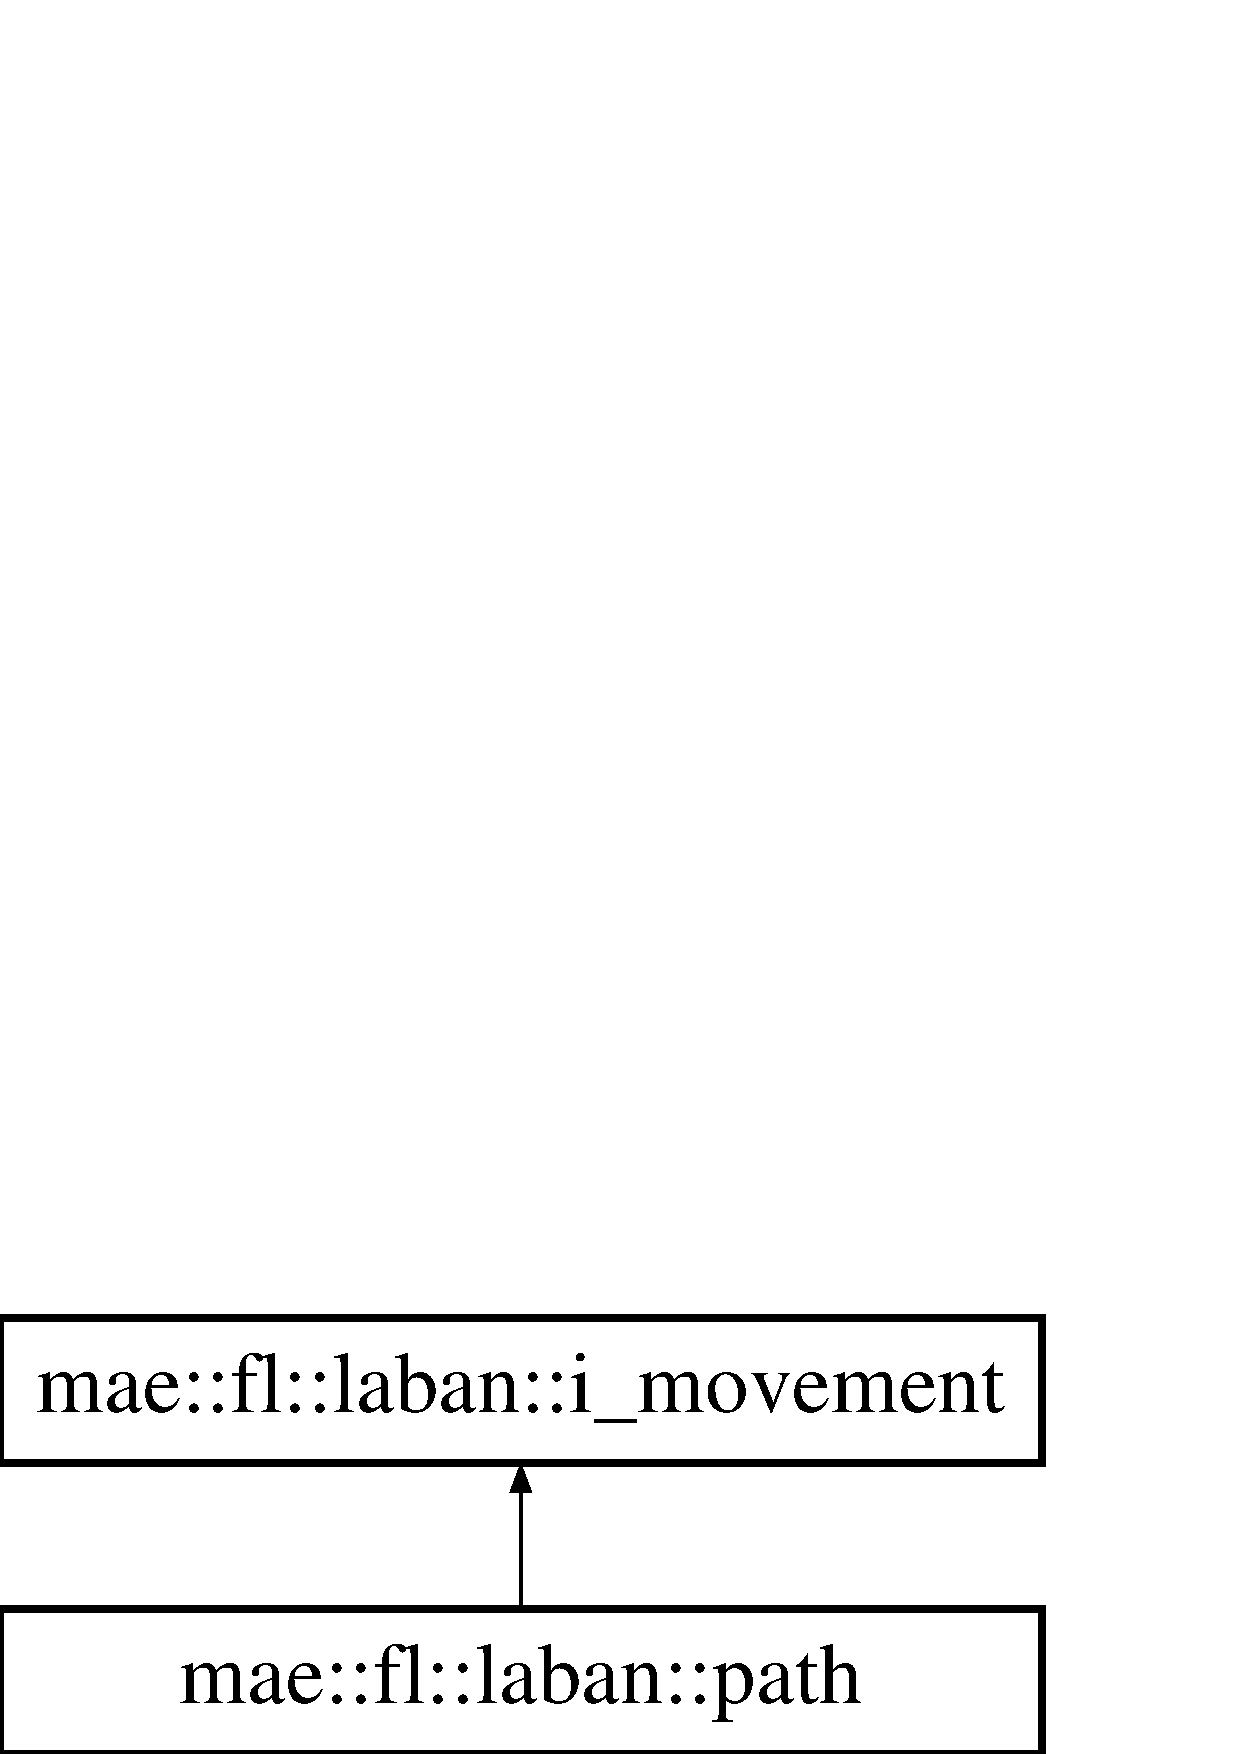
\includegraphics[height=2.000000cm]{classmae_1_1fl_1_1laban_1_1path}
\end{center}
\end{figure}
\subsection*{Public Member Functions}
\begin{DoxyCompactItemize}
\item 
\hyperlink{classmae_1_1fl_1_1laban_1_1path_a68f460107949210973195837c9f1b33c}{path} (e\-\_\-path\-\_\-type type, unsigned int measure, double beat, double duration)
\item 
e\-\_\-path\-\_\-type \hyperlink{classmae_1_1fl_1_1laban_1_1path_ac9698b90c1d5dae5d2fbc09b0db79c8d}{get\-\_\-type} () const 
\item 
virtual int \hyperlink{classmae_1_1fl_1_1laban_1_1path_a6a842cc38fccadb4d9deca546fce3e63}{get\-\_\-column} () const 
\item 
virtual unsigned int \hyperlink{classmae_1_1fl_1_1laban_1_1path_a2f355b941253903aff22add92e00124f}{get\-\_\-measure} () const 
\item 
virtual double \hyperlink{classmae_1_1fl_1_1laban_1_1path_ad7f035766edfa9f6f9f2037c26fc3309}{get\-\_\-beat} () const 
\item 
virtual double \hyperlink{classmae_1_1fl_1_1laban_1_1path_a4f45bad78535e21149bdec9a48067113}{get\-\_\-duration} () const 
\item 
virtual bool \hyperlink{classmae_1_1fl_1_1laban_1_1path_ade22858a457d91a3faa2a3eee14d66be}{equals} (std\-::shared\-\_\-ptr$<$ \hyperlink{classmae_1_1fl_1_1laban_1_1i__movement}{i\-\_\-movement} $>$ a) const 
\item 
virtual bool \hyperlink{classmae_1_1fl_1_1laban_1_1path_a209b3fe2e8df9d2c98999684bed7f496}{symbol\-\_\-equals} (std\-::shared\-\_\-ptr$<$ \hyperlink{classmae_1_1fl_1_1laban_1_1i__movement}{i\-\_\-movement} $>$ a) const 
\item 
virtual std\-::string \hyperlink{classmae_1_1fl_1_1laban_1_1path_a20f5c424a4fc9036a66a7a6f806940f4}{xml} (unsigned int indent=0, std\-::string namesp=\char`\"{}\char`\"{}) const 
\item 
virtual std\-::string \hyperlink{classmae_1_1fl_1_1laban_1_1path_a5503bfcfc2a9461b48a3bd2232918d88}{svg} (unsigned int im\-\_\-width, unsigned int im\-\_\-height, unsigned int max\-\_\-column, unsigned int measures, unsigned int beats\-\_\-per\-\_\-measure) const 
\item 
virtual std\-::shared\-\_\-ptr\\*
$<$ \hyperlink{classmae_1_1fl_1_1laban_1_1i__movement}{i\-\_\-movement} $>$ \hyperlink{classmae_1_1fl_1_1laban_1_1path_a3454902829d0ae3a3e958d59cce9cd47}{recreate} (std\-::map$<$ int, int $>$ column\-\_\-mapping, unsigned int measure, double beat, double duration) const 
\item 
virtual std\-::string \hyperlink{classmae_1_1fl_1_1laban_1_1path_a4824d4b55eac3e255a64537be864fc24}{str} () const 
\end{DoxyCompactItemize}
\subsection*{Friends}
\begin{DoxyCompactItemize}
\item 
\hypertarget{classmae_1_1fl_1_1laban_1_1path_aceed710caa3bc637e9e6df7ba92b080e}{std\-::ostream \& {\bfseries operator$<$$<$} (std\-::ostream \&os, const \hyperlink{classmae_1_1fl_1_1laban_1_1path}{path} \&obj)}\label{classmae_1_1fl_1_1laban_1_1path_aceed710caa3bc637e9e6df7ba92b080e}

\item 
\hypertarget{classmae_1_1fl_1_1laban_1_1path_aa1a1a4bcea7af934506f3e3f1111af83}{std\-::ostream \& {\bfseries operator$<$$<$} (std\-::ostream \&os, const std\-::shared\-\_\-ptr$<$ \hyperlink{classmae_1_1fl_1_1laban_1_1path}{path} $>$ \&obj)}\label{classmae_1_1fl_1_1laban_1_1path_aa1a1a4bcea7af934506f3e3f1111af83}

\end{DoxyCompactItemize}


\subsection{Constructor \& Destructor Documentation}
\hypertarget{classmae_1_1fl_1_1laban_1_1path_a68f460107949210973195837c9f1b33c}{\index{mae\-::fl\-::laban\-::path@{mae\-::fl\-::laban\-::path}!path@{path}}
\index{path@{path}!mae::fl::laban::path@{mae\-::fl\-::laban\-::path}}
\subsubsection[{path}]{\setlength{\rightskip}{0pt plus 5cm}mae\-::fl\-::laban\-::path\-::path (
\begin{DoxyParamCaption}
\item[{e\-\_\-path\-\_\-type}]{type, }
\item[{unsigned int}]{measure, }
\item[{double}]{beat, }
\item[{double}]{duration}
\end{DoxyParamCaption}
)}}\label{classmae_1_1fl_1_1laban_1_1path_a68f460107949210973195837c9f1b33c}
Creates a path symbol.


\begin{DoxyParams}{Parameters}
{\em type} & The type of the path. \\
\hline
{\em measure} & The measure in which this symbol is placed. \\
\hline
{\em beat} & The beat mark of the measure where this symbol begins. \\
\hline
{\em duration} & The duration of the symbol (in beats). \\
\hline
\end{DoxyParams}


\subsection{Member Function Documentation}
\hypertarget{classmae_1_1fl_1_1laban_1_1path_ade22858a457d91a3faa2a3eee14d66be}{\index{mae\-::fl\-::laban\-::path@{mae\-::fl\-::laban\-::path}!equals@{equals}}
\index{equals@{equals}!mae::fl::laban::path@{mae\-::fl\-::laban\-::path}}
\subsubsection[{equals}]{\setlength{\rightskip}{0pt plus 5cm}bool mae\-::fl\-::laban\-::path\-::equals (
\begin{DoxyParamCaption}
\item[{std\-::shared\-\_\-ptr$<$ {\bf i\-\_\-movement} $>$}]{a}
\end{DoxyParamCaption}
) const\hspace{0.3cm}{\ttfamily [virtual]}}}\label{classmae_1_1fl_1_1laban_1_1path_ade22858a457d91a3faa2a3eee14d66be}
Returns true if the \hyperlink{classmae_1_1fl_1_1laban_1_1i__movement}{i\-\_\-movement} elements are equal.


\begin{DoxyParams}{Parameters}
{\em a} & The movement to be compared to. \\
\hline
\end{DoxyParams}
\begin{DoxyReturn}{Returns}
True if equal. 
\end{DoxyReturn}


Implements \hyperlink{classmae_1_1fl_1_1laban_1_1i__movement_a29783771372283ff2cc7deded01b83b1}{mae\-::fl\-::laban\-::i\-\_\-movement}.

\hypertarget{classmae_1_1fl_1_1laban_1_1path_ad7f035766edfa9f6f9f2037c26fc3309}{\index{mae\-::fl\-::laban\-::path@{mae\-::fl\-::laban\-::path}!get\-\_\-beat@{get\-\_\-beat}}
\index{get\-\_\-beat@{get\-\_\-beat}!mae::fl::laban::path@{mae\-::fl\-::laban\-::path}}
\subsubsection[{get\-\_\-beat}]{\setlength{\rightskip}{0pt plus 5cm}double mae\-::fl\-::laban\-::path\-::get\-\_\-beat (
\begin{DoxyParamCaption}
{}
\end{DoxyParamCaption}
) const\hspace{0.3cm}{\ttfamily [virtual]}}}\label{classmae_1_1fl_1_1laban_1_1path_ad7f035766edfa9f6f9f2037c26fc3309}
Returns the beat where this symbol starts. \begin{DoxyReturn}{Returns}

\end{DoxyReturn}


Implements \hyperlink{classmae_1_1fl_1_1laban_1_1i__movement_a2b8ee7b4d5cb5be09be93ff049fbdc68}{mae\-::fl\-::laban\-::i\-\_\-movement}.

\hypertarget{classmae_1_1fl_1_1laban_1_1path_a6a842cc38fccadb4d9deca546fce3e63}{\index{mae\-::fl\-::laban\-::path@{mae\-::fl\-::laban\-::path}!get\-\_\-column@{get\-\_\-column}}
\index{get\-\_\-column@{get\-\_\-column}!mae::fl::laban::path@{mae\-::fl\-::laban\-::path}}
\subsubsection[{get\-\_\-column}]{\setlength{\rightskip}{0pt plus 5cm}int mae\-::fl\-::laban\-::path\-::get\-\_\-column (
\begin{DoxyParamCaption}
{}
\end{DoxyParamCaption}
) const\hspace{0.3cm}{\ttfamily [virtual]}}}\label{classmae_1_1fl_1_1laban_1_1path_a6a842cc38fccadb4d9deca546fce3e63}
Returns the column to which this symbol was added. Since a path symbol is placed in its own column zero is returned.

\begin{DoxyReturn}{Returns}
Zero. 
\end{DoxyReturn}


Implements \hyperlink{classmae_1_1fl_1_1laban_1_1i__movement_a448424f76457ed1dfa28e5d2c774c311}{mae\-::fl\-::laban\-::i\-\_\-movement}.

\hypertarget{classmae_1_1fl_1_1laban_1_1path_a4f45bad78535e21149bdec9a48067113}{\index{mae\-::fl\-::laban\-::path@{mae\-::fl\-::laban\-::path}!get\-\_\-duration@{get\-\_\-duration}}
\index{get\-\_\-duration@{get\-\_\-duration}!mae::fl::laban::path@{mae\-::fl\-::laban\-::path}}
\subsubsection[{get\-\_\-duration}]{\setlength{\rightskip}{0pt plus 5cm}double mae\-::fl\-::laban\-::path\-::get\-\_\-duration (
\begin{DoxyParamCaption}
{}
\end{DoxyParamCaption}
) const\hspace{0.3cm}{\ttfamily [virtual]}}}\label{classmae_1_1fl_1_1laban_1_1path_a4f45bad78535e21149bdec9a48067113}
Returns the duration of the symbol in beats.

\begin{DoxyReturn}{Returns}

\end{DoxyReturn}


Implements \hyperlink{classmae_1_1fl_1_1laban_1_1i__movement_ac83194ad9df8fed6c27199e83d35460d}{mae\-::fl\-::laban\-::i\-\_\-movement}.

\hypertarget{classmae_1_1fl_1_1laban_1_1path_a2f355b941253903aff22add92e00124f}{\index{mae\-::fl\-::laban\-::path@{mae\-::fl\-::laban\-::path}!get\-\_\-measure@{get\-\_\-measure}}
\index{get\-\_\-measure@{get\-\_\-measure}!mae::fl::laban::path@{mae\-::fl\-::laban\-::path}}
\subsubsection[{get\-\_\-measure}]{\setlength{\rightskip}{0pt plus 5cm}unsigned int mae\-::fl\-::laban\-::path\-::get\-\_\-measure (
\begin{DoxyParamCaption}
{}
\end{DoxyParamCaption}
) const\hspace{0.3cm}{\ttfamily [virtual]}}}\label{classmae_1_1fl_1_1laban_1_1path_a2f355b941253903aff22add92e00124f}
Returns the measure in which this symbol is placed. \begin{DoxyReturn}{Returns}

\end{DoxyReturn}


Implements \hyperlink{classmae_1_1fl_1_1laban_1_1i__movement_aa1b18a889adea3d1aa8a5a8af5de2de6}{mae\-::fl\-::laban\-::i\-\_\-movement}.

\hypertarget{classmae_1_1fl_1_1laban_1_1path_ac9698b90c1d5dae5d2fbc09b0db79c8d}{\index{mae\-::fl\-::laban\-::path@{mae\-::fl\-::laban\-::path}!get\-\_\-type@{get\-\_\-type}}
\index{get\-\_\-type@{get\-\_\-type}!mae::fl::laban::path@{mae\-::fl\-::laban\-::path}}
\subsubsection[{get\-\_\-type}]{\setlength{\rightskip}{0pt plus 5cm}e\-\_\-path\-\_\-type mae\-::fl\-::laban\-::path\-::get\-\_\-type (
\begin{DoxyParamCaption}
{}
\end{DoxyParamCaption}
) const}}\label{classmae_1_1fl_1_1laban_1_1path_ac9698b90c1d5dae5d2fbc09b0db79c8d}
Returns the type of the path.

\begin{DoxyReturn}{Returns}

\end{DoxyReturn}
\hypertarget{classmae_1_1fl_1_1laban_1_1path_a3454902829d0ae3a3e958d59cce9cd47}{\index{mae\-::fl\-::laban\-::path@{mae\-::fl\-::laban\-::path}!recreate@{recreate}}
\index{recreate@{recreate}!mae::fl::laban::path@{mae\-::fl\-::laban\-::path}}
\subsubsection[{recreate}]{\setlength{\rightskip}{0pt plus 5cm}std\-::shared\-\_\-ptr$<$ {\bf i\-\_\-movement} $>$ mae\-::fl\-::laban\-::path\-::recreate (
\begin{DoxyParamCaption}
\item[{std\-::map$<$ int, int $>$}]{column\-\_\-mapping, }
\item[{unsigned int}]{measure, }
\item[{double}]{beat, }
\item[{double}]{duration}
\end{DoxyParamCaption}
) const\hspace{0.3cm}{\ttfamily [virtual]}}}\label{classmae_1_1fl_1_1laban_1_1path_a3454902829d0ae3a3e958d59cce9cd47}
Recreates the movement by copying its members but changing the position in the staff.


\begin{DoxyParams}{Parameters}
{\em column} & The new column. \\
\hline
{\em measure} & The new measure. \\
\hline
{\em beat} & The new beat. \\
\hline
{\em duration} & The new duration. \\
\hline
\end{DoxyParams}
\begin{DoxyReturn}{Returns}
The new, recreated movement. 
\end{DoxyReturn}


Implements \hyperlink{classmae_1_1fl_1_1laban_1_1i__movement_a28c8b00c68e291399281bda22e4f01f6}{mae\-::fl\-::laban\-::i\-\_\-movement}.

\hypertarget{classmae_1_1fl_1_1laban_1_1path_a4824d4b55eac3e255a64537be864fc24}{\index{mae\-::fl\-::laban\-::path@{mae\-::fl\-::laban\-::path}!str@{str}}
\index{str@{str}!mae::fl::laban::path@{mae\-::fl\-::laban\-::path}}
\subsubsection[{str}]{\setlength{\rightskip}{0pt plus 5cm}std\-::string mae\-::fl\-::laban\-::path\-::str (
\begin{DoxyParamCaption}
{}
\end{DoxyParamCaption}
) const\hspace{0.3cm}{\ttfamily [virtual]}}}\label{classmae_1_1fl_1_1laban_1_1path_a4824d4b55eac3e255a64537be864fc24}
Returns the string representation for this element.

\begin{DoxyReturn}{Returns}
The string. 
\end{DoxyReturn}


Implements \hyperlink{classmae_1_1fl_1_1laban_1_1i__movement_a18322189d1851d3fd0f85c00b1051b57}{mae\-::fl\-::laban\-::i\-\_\-movement}.

\hypertarget{classmae_1_1fl_1_1laban_1_1path_a5503bfcfc2a9461b48a3bd2232918d88}{\index{mae\-::fl\-::laban\-::path@{mae\-::fl\-::laban\-::path}!svg@{svg}}
\index{svg@{svg}!mae::fl::laban::path@{mae\-::fl\-::laban\-::path}}
\subsubsection[{svg}]{\setlength{\rightskip}{0pt plus 5cm}std\-::string mae\-::fl\-::laban\-::path\-::svg (
\begin{DoxyParamCaption}
\item[{unsigned int}]{im\-\_\-width, }
\item[{unsigned int}]{im\-\_\-height, }
\item[{unsigned int}]{max\-\_\-column, }
\item[{unsigned int}]{measures, }
\item[{unsigned int}]{beats\-\_\-per\-\_\-measure}
\end{DoxyParamCaption}
) const\hspace{0.3cm}{\ttfamily [virtual]}}}\label{classmae_1_1fl_1_1laban_1_1path_a5503bfcfc2a9461b48a3bd2232918d88}
Returns the S\-V\-G representation for this element.


\begin{DoxyParams}{Parameters}
{\em posx} & The x pos. \\
\hline
{\em posy} & The y pos. \\
\hline
{\em width} & The width. \\
\hline
{\em height} & The height. \\
\hline
\end{DoxyParams}
\begin{DoxyReturn}{Returns}
The S\-V\-G. 
\end{DoxyReturn}


Implements \hyperlink{classmae_1_1fl_1_1laban_1_1i__movement_ab2b0225ae8237b8ae410c797a0319498}{mae\-::fl\-::laban\-::i\-\_\-movement}.

\hypertarget{classmae_1_1fl_1_1laban_1_1path_a209b3fe2e8df9d2c98999684bed7f496}{\index{mae\-::fl\-::laban\-::path@{mae\-::fl\-::laban\-::path}!symbol\-\_\-equals@{symbol\-\_\-equals}}
\index{symbol\-\_\-equals@{symbol\-\_\-equals}!mae::fl::laban::path@{mae\-::fl\-::laban\-::path}}
\subsubsection[{symbol\-\_\-equals}]{\setlength{\rightskip}{0pt plus 5cm}bool mae\-::fl\-::laban\-::path\-::symbol\-\_\-equals (
\begin{DoxyParamCaption}
\item[{std\-::shared\-\_\-ptr$<$ {\bf i\-\_\-movement} $>$}]{a}
\end{DoxyParamCaption}
) const\hspace{0.3cm}{\ttfamily [virtual]}}}\label{classmae_1_1fl_1_1laban_1_1path_a209b3fe2e8df9d2c98999684bed7f496}
Returns true if the symbols are equal. The position and duration are not regarded.


\begin{DoxyParams}{Parameters}
{\em a} & The movement to be compared to. \\
\hline
\end{DoxyParams}
\begin{DoxyReturn}{Returns}
True if symbols equal. 
\end{DoxyReturn}


Implements \hyperlink{classmae_1_1fl_1_1laban_1_1i__movement_a7b682911356dd13497172280b268ec40}{mae\-::fl\-::laban\-::i\-\_\-movement}.

\hypertarget{classmae_1_1fl_1_1laban_1_1path_a20f5c424a4fc9036a66a7a6f806940f4}{\index{mae\-::fl\-::laban\-::path@{mae\-::fl\-::laban\-::path}!xml@{xml}}
\index{xml@{xml}!mae::fl::laban::path@{mae\-::fl\-::laban\-::path}}
\subsubsection[{xml}]{\setlength{\rightskip}{0pt plus 5cm}std\-::string mae\-::fl\-::laban\-::path\-::xml (
\begin{DoxyParamCaption}
\item[{unsigned int}]{indent = {\ttfamily 0}, }
\item[{std\-::string}]{namesp = {\ttfamily \char`\"{}\char`\"{}}}
\end{DoxyParamCaption}
) const\hspace{0.3cm}{\ttfamily [virtual]}}}\label{classmae_1_1fl_1_1laban_1_1path_a20f5c424a4fc9036a66a7a6f806940f4}
Returns the X\-M\-L representation for this element.


\begin{DoxyParams}{Parameters}
{\em indent} & The applied indent. \\
\hline
{\em namesp} & The prefixed X\-M\-L namespace.\\
\hline
\end{DoxyParams}
\begin{DoxyReturn}{Returns}
The X\-M\-L string. 
\end{DoxyReturn}


Implements \hyperlink{classmae_1_1fl_1_1laban_1_1i__movement_acd832b2a6976bfe32eae4bece01ee8f3}{mae\-::fl\-::laban\-::i\-\_\-movement}.



The documentation for this class was generated from the following files\-:\begin{DoxyCompactItemize}
\item 
src/mae/fl/laban/path.\-hpp\item 
src/mae/fl/laban/path.\-cpp\end{DoxyCompactItemize}

\hypertarget{classmae_1_1fl_1_1laban_1_1mv_1_1pin}{\section{mae\-:\-:fl\-:\-:laban\-:\-:mv\-:\-:pin Class Reference}
\label{classmae_1_1fl_1_1laban_1_1mv_1_1pin}\index{mae\-::fl\-::laban\-::mv\-::pin@{mae\-::fl\-::laban\-::mv\-::pin}}
}
Inheritance diagram for mae\-:\-:fl\-:\-:laban\-:\-:mv\-:\-:pin\-:\begin{figure}[H]
\begin{center}
\leavevmode
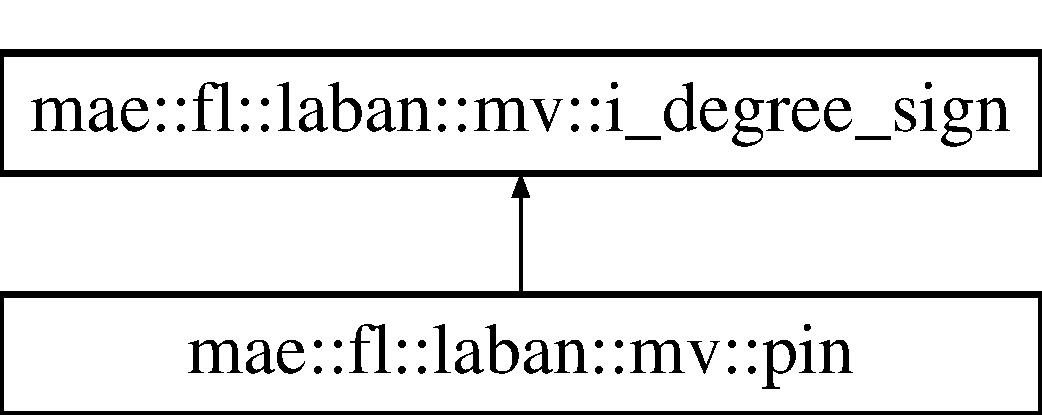
\includegraphics[height=2.000000cm]{classmae_1_1fl_1_1laban_1_1mv_1_1pin}
\end{center}
\end{figure}
\subsection*{Public Member Functions}
\begin{DoxyCompactItemize}
\item 
\hyperlink{classmae_1_1fl_1_1laban_1_1mv_1_1pin_a07a30c5fa556e83f4bf5884e35511ae4}{pin} (e\-\_\-level level, int horizontal)
\item 
e\-\_\-level \hyperlink{classmae_1_1fl_1_1laban_1_1mv_1_1pin_a2b6dd6bdc2a2642abf265bee1a111cf3}{get\-\_\-level} () const 
\item 
int \hyperlink{classmae_1_1fl_1_1laban_1_1mv_1_1pin_aa93e5de8f1ad1ab6fe87157a2d0906ce}{get\-\_\-horizontal} () const 
\item 
virtual bool \hyperlink{classmae_1_1fl_1_1laban_1_1mv_1_1pin_a49353682e373a913730f0556f8fe2963}{equals} (std\-::shared\-\_\-ptr$<$ \hyperlink{classmae_1_1fl_1_1laban_1_1mv_1_1i__degree__sign}{i\-\_\-degree\-\_\-sign} $>$ a) const 
\item 
virtual std\-::string \hyperlink{classmae_1_1fl_1_1laban_1_1mv_1_1pin_a1a253c5718b0f88e4ffb8bf06e8bff22}{xml} (unsigned int indent=0, std\-::string namesp=\char`\"{}\char`\"{}, bool print\-\_\-type=false) const 
\item 
virtual std\-::string \hyperlink{classmae_1_1fl_1_1laban_1_1mv_1_1pin_ae4af4900e50fc252ecd151da4ad2fe2a}{svg} (std\-::string identifier, double posx, double posy, double width, double height, bool left=false) const 
\end{DoxyCompactItemize}


\subsection{Constructor \& Destructor Documentation}
\hypertarget{classmae_1_1fl_1_1laban_1_1mv_1_1pin_a07a30c5fa556e83f4bf5884e35511ae4}{\index{mae\-::fl\-::laban\-::mv\-::pin@{mae\-::fl\-::laban\-::mv\-::pin}!pin@{pin}}
\index{pin@{pin}!mae::fl::laban::mv::pin@{mae\-::fl\-::laban\-::mv\-::pin}}
\subsubsection[{pin}]{\setlength{\rightskip}{0pt plus 5cm}mae\-::fl\-::laban\-::mv\-::pin\-::pin (
\begin{DoxyParamCaption}
\item[{e\-\_\-level}]{level, }
\item[{int}]{horizontal}
\end{DoxyParamCaption}
)}}\label{classmae_1_1fl_1_1laban_1_1mv_1_1pin_a07a30c5fa556e83f4bf5884e35511ae4}
Creates a pin. The horizontal direction must be a value between -\/1 and 360.


\begin{DoxyParams}{Parameters}
{\em level} & The level type. \\
\hline
{\em horizontal} & The horizontal direction which must be a value between -\/1 and 360. -\/1 represents at place whereas a value between 0 and 360 represents a the degree relative to the forward direction (e.\-g. 90 represents \char`\"{}right\char`\"{}). \\
\hline
\end{DoxyParams}


\subsection{Member Function Documentation}
\hypertarget{classmae_1_1fl_1_1laban_1_1mv_1_1pin_a49353682e373a913730f0556f8fe2963}{\index{mae\-::fl\-::laban\-::mv\-::pin@{mae\-::fl\-::laban\-::mv\-::pin}!equals@{equals}}
\index{equals@{equals}!mae::fl::laban::mv::pin@{mae\-::fl\-::laban\-::mv\-::pin}}
\subsubsection[{equals}]{\setlength{\rightskip}{0pt plus 5cm}bool mae\-::fl\-::laban\-::mv\-::pin\-::equals (
\begin{DoxyParamCaption}
\item[{std\-::shared\-\_\-ptr$<$ {\bf i\-\_\-degree\-\_\-sign} $>$}]{a}
\end{DoxyParamCaption}
) const\hspace{0.3cm}{\ttfamily [virtual]}}}\label{classmae_1_1fl_1_1laban_1_1mv_1_1pin_a49353682e373a913730f0556f8fe2963}
Returns true if signs are equal.


\begin{DoxyParams}{Parameters}
{\em a} & The sign to be compared to. \\
\hline
\end{DoxyParams}
\begin{DoxyReturn}{Returns}
True if equal. 
\end{DoxyReturn}


Implements \hyperlink{classmae_1_1fl_1_1laban_1_1mv_1_1i__degree__sign_a65fee11b31d29709fd4022f90f4638bd}{mae\-::fl\-::laban\-::mv\-::i\-\_\-degree\-\_\-sign}.

\hypertarget{classmae_1_1fl_1_1laban_1_1mv_1_1pin_aa93e5de8f1ad1ab6fe87157a2d0906ce}{\index{mae\-::fl\-::laban\-::mv\-::pin@{mae\-::fl\-::laban\-::mv\-::pin}!get\-\_\-horizontal@{get\-\_\-horizontal}}
\index{get\-\_\-horizontal@{get\-\_\-horizontal}!mae::fl::laban::mv::pin@{mae\-::fl\-::laban\-::mv\-::pin}}
\subsubsection[{get\-\_\-horizontal}]{\setlength{\rightskip}{0pt plus 5cm}int mae\-::fl\-::laban\-::mv\-::pin\-::get\-\_\-horizontal (
\begin{DoxyParamCaption}
{}
\end{DoxyParamCaption}
) const}}\label{classmae_1_1fl_1_1laban_1_1mv_1_1pin_aa93e5de8f1ad1ab6fe87157a2d0906ce}
Returns the (horizontal) direction which is a value between -\/1 and 360. -\/1 represents at place whereas a value between 0 and 360 represents a the degree relative to the forward direction (e.\-g. 90 represents \char`\"{}right\char`\"{}).

\begin{DoxyReturn}{Returns}
The direction. 
\end{DoxyReturn}
\hypertarget{classmae_1_1fl_1_1laban_1_1mv_1_1pin_a2b6dd6bdc2a2642abf265bee1a111cf3}{\index{mae\-::fl\-::laban\-::mv\-::pin@{mae\-::fl\-::laban\-::mv\-::pin}!get\-\_\-level@{get\-\_\-level}}
\index{get\-\_\-level@{get\-\_\-level}!mae::fl::laban::mv::pin@{mae\-::fl\-::laban\-::mv\-::pin}}
\subsubsection[{get\-\_\-level}]{\setlength{\rightskip}{0pt plus 5cm}e\-\_\-level mae\-::fl\-::laban\-::mv\-::pin\-::get\-\_\-level (
\begin{DoxyParamCaption}
{}
\end{DoxyParamCaption}
) const}}\label{classmae_1_1fl_1_1laban_1_1mv_1_1pin_a2b6dd6bdc2a2642abf265bee1a111cf3}
Returns the level.

\begin{DoxyReturn}{Returns}
The level. 
\end{DoxyReturn}
\hypertarget{classmae_1_1fl_1_1laban_1_1mv_1_1pin_ae4af4900e50fc252ecd151da4ad2fe2a}{\index{mae\-::fl\-::laban\-::mv\-::pin@{mae\-::fl\-::laban\-::mv\-::pin}!svg@{svg}}
\index{svg@{svg}!mae::fl::laban::mv::pin@{mae\-::fl\-::laban\-::mv\-::pin}}
\subsubsection[{svg}]{\setlength{\rightskip}{0pt plus 5cm}std\-::string mae\-::fl\-::laban\-::mv\-::pin\-::svg (
\begin{DoxyParamCaption}
\item[{std\-::string}]{identifier, }
\item[{double}]{posx, }
\item[{double}]{posy, }
\item[{double}]{width, }
\item[{double}]{height, }
\item[{bool}]{left = {\ttfamily false}}
\end{DoxyParamCaption}
) const\hspace{0.3cm}{\ttfamily [virtual]}}}\label{classmae_1_1fl_1_1laban_1_1mv_1_1pin_ae4af4900e50fc252ecd151da4ad2fe2a}
Returns the S\-V\-G representation for this symbol.


\begin{DoxyParams}{Parameters}
{\em posx} & The x position. \\
\hline
{\em posy} & The y position. \\
\hline
{\em width} & The width. \\
\hline
{\em height} & The height. \\
\hline
\end{DoxyParams}
\begin{DoxyReturn}{Returns}
The S\-V\-G. 
\end{DoxyReturn}


Implements \hyperlink{classmae_1_1fl_1_1laban_1_1mv_1_1i__degree__sign_abb3ff23c8dcaaa80b6062bf5f8162c51}{mae\-::fl\-::laban\-::mv\-::i\-\_\-degree\-\_\-sign}.

\hypertarget{classmae_1_1fl_1_1laban_1_1mv_1_1pin_a1a253c5718b0f88e4ffb8bf06e8bff22}{\index{mae\-::fl\-::laban\-::mv\-::pin@{mae\-::fl\-::laban\-::mv\-::pin}!xml@{xml}}
\index{xml@{xml}!mae::fl::laban::mv::pin@{mae\-::fl\-::laban\-::mv\-::pin}}
\subsubsection[{xml}]{\setlength{\rightskip}{0pt plus 5cm}std\-::string mae\-::fl\-::laban\-::mv\-::pin\-::xml (
\begin{DoxyParamCaption}
\item[{unsigned int}]{indent = {\ttfamily 0}, }
\item[{std\-::string}]{namesp = {\ttfamily \char`\"{}\char`\"{}}, }
\item[{bool}]{print\-\_\-type = {\ttfamily false}}
\end{DoxyParamCaption}
) const\hspace{0.3cm}{\ttfamily [virtual]}}}\label{classmae_1_1fl_1_1laban_1_1mv_1_1pin_a1a253c5718b0f88e4ffb8bf06e8bff22}
Returns the X\-M\-L representation for this element.


\begin{DoxyParams}{Parameters}
{\em indent} & The applied indent. \\
\hline
{\em namesp} & The prefixed X\-M\-L namespace.\\
\hline
\end{DoxyParams}
\begin{DoxyReturn}{Returns}
The X\-M\-L string. 
\end{DoxyReturn}


Implements \hyperlink{classmae_1_1fl_1_1laban_1_1mv_1_1i__degree__sign_abddf8459a5231b204ac2f023633aa4c4}{mae\-::fl\-::laban\-::mv\-::i\-\_\-degree\-\_\-sign}.



The documentation for this class was generated from the following files\-:\begin{DoxyCompactItemize}
\item 
src/mae/fl/laban/mv/pin.\-hpp\item 
src/mae/fl/laban/mv/pin.\-cpp\end{DoxyCompactItemize}

\hypertarget{classmae_1_1fl_1_1laban_1_1ps_1_1prop}{\section{mae\-:\-:fl\-:\-:laban\-:\-:ps\-:\-:prop Class Reference}
\label{classmae_1_1fl_1_1laban_1_1ps_1_1prop}\index{mae\-::fl\-::laban\-::ps\-::prop@{mae\-::fl\-::laban\-::ps\-::prop}}
}
Inheritance diagram for mae\-:\-:fl\-:\-:laban\-:\-:ps\-:\-:prop\-:\begin{figure}[H]
\begin{center}
\leavevmode
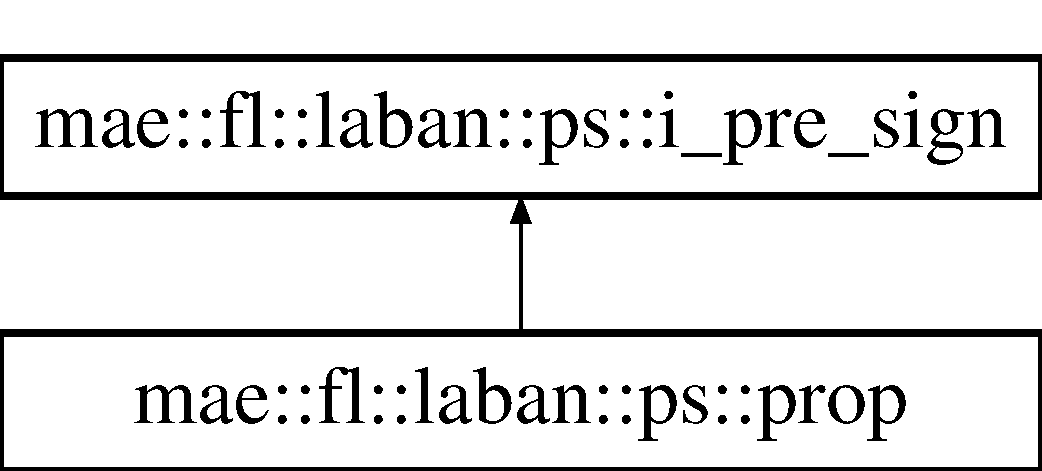
\includegraphics[height=2.000000cm]{classmae_1_1fl_1_1laban_1_1ps_1_1prop}
\end{center}
\end{figure}
\subsection*{Public Member Functions}
\begin{DoxyCompactItemize}
\item 
\hyperlink{classmae_1_1fl_1_1laban_1_1ps_1_1prop_aa718f11fd36340cdaa1838989b3a1ebf}{prop} (std\-::string name, std\-::string description=\char`\"{}\char`\"{})
\item 
std\-::string \hyperlink{classmae_1_1fl_1_1laban_1_1ps_1_1prop_a369d172ed15a16f5d6ef3d442056987f}{get\-\_\-name} () const 
\item 
std\-::string \hyperlink{classmae_1_1fl_1_1laban_1_1ps_1_1prop_aa9f90e69ede9253c8bb1cddba6799843}{get\-\_\-description} () const 
\item 
virtual std\-::string \hyperlink{classmae_1_1fl_1_1laban_1_1ps_1_1prop_a075d19bb27eeb7cc4d1af8a5294a3507}{xml} (unsigned int indent=0, std\-::string namesp=\char`\"{}\char`\"{}) const 
\item 
virtual std\-::string \hyperlink{classmae_1_1fl_1_1laban_1_1ps_1_1prop_ae0439113058f4ed15bc3826f3e93e6d9}{svg} (std\-::string identifier, double posx, double posy, double width, double height, bool left=false) const 
\item 
virtual bool \hyperlink{classmae_1_1fl_1_1laban_1_1ps_1_1prop_a03b8c4bfa1731767fe0c868555c17c1b}{equals} (std\-::shared\-\_\-ptr$<$ \hyperlink{classmae_1_1fl_1_1laban_1_1ps_1_1i__pre__sign}{i\-\_\-pre\-\_\-sign} $>$ a) const 
\end{DoxyCompactItemize}


\subsection{Constructor \& Destructor Documentation}
\hypertarget{classmae_1_1fl_1_1laban_1_1ps_1_1prop_aa718f11fd36340cdaa1838989b3a1ebf}{\index{mae\-::fl\-::laban\-::ps\-::prop@{mae\-::fl\-::laban\-::ps\-::prop}!prop@{prop}}
\index{prop@{prop}!mae::fl::laban::ps::prop@{mae\-::fl\-::laban\-::ps\-::prop}}
\subsubsection[{prop}]{\setlength{\rightskip}{0pt plus 5cm}mae\-::fl\-::laban\-::ps\-::prop\-::prop (
\begin{DoxyParamCaption}
\item[{std\-::string}]{name, }
\item[{std\-::string}]{description = {\ttfamily \char`\"{}\char`\"{}}}
\end{DoxyParamCaption}
)}}\label{classmae_1_1fl_1_1laban_1_1ps_1_1prop_aa718f11fd36340cdaa1838989b3a1ebf}
Creates a prop pre-\/sign which can be used to freely define a pre-\/sign using a name and an optional description.


\begin{DoxyParams}{Parameters}
{\em name} & The expressive name of the pre-\/sign. \\
\hline
{\em description} & The optional description. \\
\hline
\end{DoxyParams}


\subsection{Member Function Documentation}
\hypertarget{classmae_1_1fl_1_1laban_1_1ps_1_1prop_a03b8c4bfa1731767fe0c868555c17c1b}{\index{mae\-::fl\-::laban\-::ps\-::prop@{mae\-::fl\-::laban\-::ps\-::prop}!equals@{equals}}
\index{equals@{equals}!mae::fl::laban::ps::prop@{mae\-::fl\-::laban\-::ps\-::prop}}
\subsubsection[{equals}]{\setlength{\rightskip}{0pt plus 5cm}bool mae\-::fl\-::laban\-::ps\-::prop\-::equals (
\begin{DoxyParamCaption}
\item[{std\-::shared\-\_\-ptr$<$ {\bf i\-\_\-pre\-\_\-sign} $>$}]{a}
\end{DoxyParamCaption}
) const\hspace{0.3cm}{\ttfamily [virtual]}}}\label{classmae_1_1fl_1_1laban_1_1ps_1_1prop_a03b8c4bfa1731767fe0c868555c17c1b}
Returns true if elements are equal.


\begin{DoxyParams}{Parameters}
{\em a} & The element to be compared to. \\
\hline
\end{DoxyParams}
\begin{DoxyReturn}{Returns}
True if equal. 
\end{DoxyReturn}


Implements \hyperlink{classmae_1_1fl_1_1laban_1_1ps_1_1i__pre__sign_a8e3342fe33b6bd050d613330da30213d}{mae\-::fl\-::laban\-::ps\-::i\-\_\-pre\-\_\-sign}.

\hypertarget{classmae_1_1fl_1_1laban_1_1ps_1_1prop_aa9f90e69ede9253c8bb1cddba6799843}{\index{mae\-::fl\-::laban\-::ps\-::prop@{mae\-::fl\-::laban\-::ps\-::prop}!get\-\_\-description@{get\-\_\-description}}
\index{get\-\_\-description@{get\-\_\-description}!mae::fl::laban::ps::prop@{mae\-::fl\-::laban\-::ps\-::prop}}
\subsubsection[{get\-\_\-description}]{\setlength{\rightskip}{0pt plus 5cm}std\-::string mae\-::fl\-::laban\-::ps\-::prop\-::get\-\_\-description (
\begin{DoxyParamCaption}
{}
\end{DoxyParamCaption}
) const}}\label{classmae_1_1fl_1_1laban_1_1ps_1_1prop_aa9f90e69ede9253c8bb1cddba6799843}
Returns the description of the pre-\/sign. Returns an empty string if none set.

\begin{DoxyReturn}{Returns}

\end{DoxyReturn}
\hypertarget{classmae_1_1fl_1_1laban_1_1ps_1_1prop_a369d172ed15a16f5d6ef3d442056987f}{\index{mae\-::fl\-::laban\-::ps\-::prop@{mae\-::fl\-::laban\-::ps\-::prop}!get\-\_\-name@{get\-\_\-name}}
\index{get\-\_\-name@{get\-\_\-name}!mae::fl::laban::ps::prop@{mae\-::fl\-::laban\-::ps\-::prop}}
\subsubsection[{get\-\_\-name}]{\setlength{\rightskip}{0pt plus 5cm}std\-::string mae\-::fl\-::laban\-::ps\-::prop\-::get\-\_\-name (
\begin{DoxyParamCaption}
{}
\end{DoxyParamCaption}
) const}}\label{classmae_1_1fl_1_1laban_1_1ps_1_1prop_a369d172ed15a16f5d6ef3d442056987f}
Returns the name of the pre-\/sign. \begin{DoxyReturn}{Returns}

\end{DoxyReturn}
\hypertarget{classmae_1_1fl_1_1laban_1_1ps_1_1prop_ae0439113058f4ed15bc3826f3e93e6d9}{\index{mae\-::fl\-::laban\-::ps\-::prop@{mae\-::fl\-::laban\-::ps\-::prop}!svg@{svg}}
\index{svg@{svg}!mae::fl::laban::ps::prop@{mae\-::fl\-::laban\-::ps\-::prop}}
\subsubsection[{svg}]{\setlength{\rightskip}{0pt plus 5cm}std\-::string mae\-::fl\-::laban\-::ps\-::prop\-::svg (
\begin{DoxyParamCaption}
\item[{std\-::string}]{identifier, }
\item[{double}]{posx, }
\item[{double}]{posy, }
\item[{double}]{width, }
\item[{double}]{height, }
\item[{bool}]{left = {\ttfamily false}}
\end{DoxyParamCaption}
) const\hspace{0.3cm}{\ttfamily [virtual]}}}\label{classmae_1_1fl_1_1laban_1_1ps_1_1prop_ae0439113058f4ed15bc3826f3e93e6d9}
Returns the S\-V\-G representation for this symbol.


\begin{DoxyParams}{Parameters}
{\em posx} & The x position. \\
\hline
{\em posy} & The y position. \\
\hline
{\em width} & The width. \\
\hline
{\em height} & The height. \\
\hline
\end{DoxyParams}
\begin{DoxyReturn}{Returns}
The S\-V\-G. 
\end{DoxyReturn}


Implements \hyperlink{classmae_1_1fl_1_1laban_1_1ps_1_1i__pre__sign_a3caa95eb1c8637f531812afe1b78bbf4}{mae\-::fl\-::laban\-::ps\-::i\-\_\-pre\-\_\-sign}.

\hypertarget{classmae_1_1fl_1_1laban_1_1ps_1_1prop_a075d19bb27eeb7cc4d1af8a5294a3507}{\index{mae\-::fl\-::laban\-::ps\-::prop@{mae\-::fl\-::laban\-::ps\-::prop}!xml@{xml}}
\index{xml@{xml}!mae::fl::laban::ps::prop@{mae\-::fl\-::laban\-::ps\-::prop}}
\subsubsection[{xml}]{\setlength{\rightskip}{0pt plus 5cm}std\-::string mae\-::fl\-::laban\-::ps\-::prop\-::xml (
\begin{DoxyParamCaption}
\item[{unsigned int}]{indent = {\ttfamily 0}, }
\item[{std\-::string}]{namesp = {\ttfamily \char`\"{}\char`\"{}}}
\end{DoxyParamCaption}
) const\hspace{0.3cm}{\ttfamily [virtual]}}}\label{classmae_1_1fl_1_1laban_1_1ps_1_1prop_a075d19bb27eeb7cc4d1af8a5294a3507}
Returns the X\-M\-L representation for this element.


\begin{DoxyParams}{Parameters}
{\em indent} & The applied indent. \\
\hline
{\em namesp} & The prefixed X\-M\-L namespace.\\
\hline
\end{DoxyParams}
\begin{DoxyReturn}{Returns}
The X\-M\-L string. 
\end{DoxyReturn}


Implements \hyperlink{classmae_1_1fl_1_1laban_1_1ps_1_1i__pre__sign_a428b08efc67bb293f0fc8b41ce40215f}{mae\-::fl\-::laban\-::ps\-::i\-\_\-pre\-\_\-sign}.



The documentation for this class was generated from the following files\-:\begin{DoxyCompactItemize}
\item 
src/mae/fl/laban/ps/prop.\-hpp\item 
src/mae/fl/laban/ps/prop.\-cpp\end{DoxyCompactItemize}

\hypertarget{classmae_1_1fl_1_1laban_1_1relationship__bow}{\section{mae\-:\-:fl\-:\-:laban\-:\-:relationship\-\_\-bow Class Reference}
\label{classmae_1_1fl_1_1laban_1_1relationship__bow}\index{mae\-::fl\-::laban\-::relationship\-\_\-bow@{mae\-::fl\-::laban\-::relationship\-\_\-bow}}
}
Inheritance diagram for mae\-:\-:fl\-:\-:laban\-:\-:relationship\-\_\-bow\-:\begin{figure}[H]
\begin{center}
\leavevmode
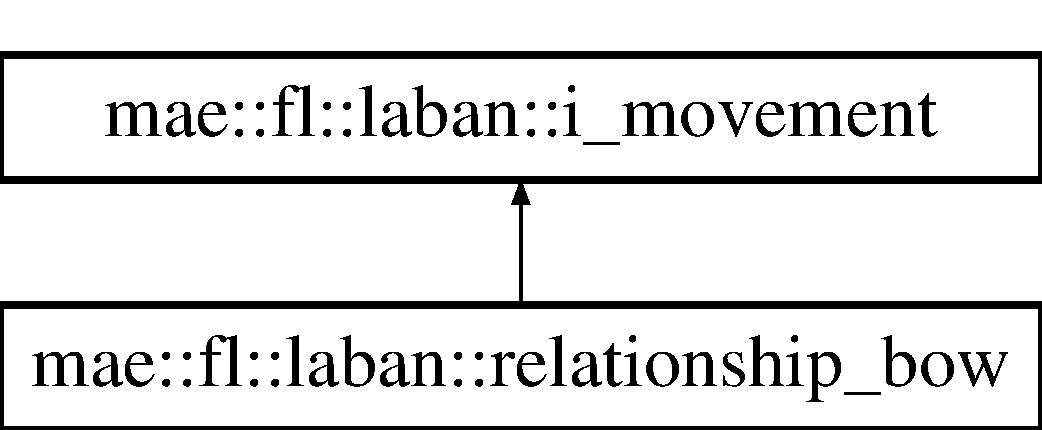
\includegraphics[height=2.000000cm]{classmae_1_1fl_1_1laban_1_1relationship__bow}
\end{center}
\end{figure}
\subsection*{Public Member Functions}
\begin{DoxyCompactItemize}
\item 
\hyperlink{classmae_1_1fl_1_1laban_1_1relationship__bow_af20f7988bf1736eab8bcfdbd5a12de89}{relationship\-\_\-bow} (e\-\_\-relationship\-\_\-type type, bool grasping, bool passing, bool hold, unsigned int measure, double beat, std\-::shared\-\_\-ptr$<$ \hyperlink{classmae_1_1fl_1_1laban_1_1mv_1_1relationship__endpoint}{mv\-::relationship\-\_\-endpoint} $>$ left\-\_\-endpoint, std\-::shared\-\_\-ptr$<$ \hyperlink{classmae_1_1fl_1_1laban_1_1mv_1_1relationship__endpoint}{mv\-::relationship\-\_\-endpoint} $>$ right\-\_\-endpoint)
\item 
e\-\_\-relationship\-\_\-type \hyperlink{classmae_1_1fl_1_1laban_1_1relationship__bow_a0e90506c82be0e73d94f4a013c432fd6}{get\-\_\-type} () const 
\item 
bool \hyperlink{classmae_1_1fl_1_1laban_1_1relationship__bow_ac5a514ef2bf7ae0b6e60ace972c7284c}{get\-\_\-grasping} () const 
\item 
bool \hyperlink{classmae_1_1fl_1_1laban_1_1relationship__bow_aa7916fd12af7c7f2d9b779f9e28cc97d}{get\-\_\-passing} () const 
\item 
bool \hyperlink{classmae_1_1fl_1_1laban_1_1relationship__bow_a78a0b9084fcd9003091126fd1d4c71d8}{get\-\_\-hold} () const 
\item 
std\-::shared\-\_\-ptr\\*
$<$ \hyperlink{classmae_1_1fl_1_1laban_1_1mv_1_1relationship__endpoint}{mv\-::relationship\-\_\-endpoint} $>$ \hyperlink{classmae_1_1fl_1_1laban_1_1relationship__bow_afd04183064710e48c50827955aef6336}{get\-\_\-left\-\_\-endpoint} () const 
\item 
std\-::shared\-\_\-ptr\\*
$<$ \hyperlink{classmae_1_1fl_1_1laban_1_1mv_1_1relationship__endpoint}{mv\-::relationship\-\_\-endpoint} $>$ \hyperlink{classmae_1_1fl_1_1laban_1_1relationship__bow_a40002c47a5b9a58005d84f19ff856921}{get\-\_\-right\-\_\-endpoint} () const 
\item 
virtual int \hyperlink{classmae_1_1fl_1_1laban_1_1relationship__bow_ada0c5d5f50bb062ba2c4a5afae33d76a}{get\-\_\-column} () const 
\item 
virtual unsigned int \hyperlink{classmae_1_1fl_1_1laban_1_1relationship__bow_af30dd493c707abfdf042a1ffe9e6d289}{get\-\_\-measure} () const 
\item 
virtual double \hyperlink{classmae_1_1fl_1_1laban_1_1relationship__bow_a0fe4d1a9fd99e3c2e5daab7c5e3ffb6a}{get\-\_\-beat} () const 
\item 
virtual double \hyperlink{classmae_1_1fl_1_1laban_1_1relationship__bow_a6d9b6feb5125d37faf2b2ef545a0b02d}{get\-\_\-duration} () const 
\item 
virtual bool \hyperlink{classmae_1_1fl_1_1laban_1_1relationship__bow_a528d367eeff4bfcff462b201187b3bfc}{equals} (std\-::shared\-\_\-ptr$<$ \hyperlink{classmae_1_1fl_1_1laban_1_1i__movement}{i\-\_\-movement} $>$ a) const 
\item 
virtual bool \hyperlink{classmae_1_1fl_1_1laban_1_1relationship__bow_afe24aac808ed21243b9d277a14adeddd}{symbol\-\_\-equals} (std\-::shared\-\_\-ptr$<$ \hyperlink{classmae_1_1fl_1_1laban_1_1i__movement}{i\-\_\-movement} $>$ a) const 
\item 
virtual std\-::string \hyperlink{classmae_1_1fl_1_1laban_1_1relationship__bow_abbeedd0547a85cbe136dce511fba09e7}{xml} (unsigned int indent=0, std\-::string namesp=\char`\"{}\char`\"{}) const 
\item 
virtual std\-::string \hyperlink{classmae_1_1fl_1_1laban_1_1relationship__bow_a8ddd7d1102dcf7989b265f7b2b50f1a1}{svg} (unsigned int im\-\_\-width, unsigned int im\-\_\-height, unsigned int max\-\_\-column, unsigned int measures, unsigned int beats\-\_\-per\-\_\-measure) const 
\item 
virtual std\-::shared\-\_\-ptr\\*
$<$ \hyperlink{classmae_1_1fl_1_1laban_1_1i__movement}{i\-\_\-movement} $>$ \hyperlink{classmae_1_1fl_1_1laban_1_1relationship__bow_a7c7cd12c0eb3dd279587f02e2eb6151f}{recreate} (std\-::map$<$ int, int $>$ column\-\_\-mapping, unsigned int measure, double beat, double duration) const 
\item 
virtual std\-::string \hyperlink{classmae_1_1fl_1_1laban_1_1relationship__bow_a704b3d739a34b7fcbf6aee9f70f474bb}{str} () const 
\end{DoxyCompactItemize}
\subsection*{Friends}
\begin{DoxyCompactItemize}
\item 
\hypertarget{classmae_1_1fl_1_1laban_1_1relationship__bow_a1b75abf13ab7a8bff7021713207afeca}{std\-::ostream \& {\bfseries operator$<$$<$} (std\-::ostream \&os, const \hyperlink{classmae_1_1fl_1_1laban_1_1relationship__bow}{relationship\-\_\-bow} \&obj)}\label{classmae_1_1fl_1_1laban_1_1relationship__bow_a1b75abf13ab7a8bff7021713207afeca}

\item 
\hypertarget{classmae_1_1fl_1_1laban_1_1relationship__bow_ae5eb7cf9d452ba6150130d77bb319a32}{std\-::ostream \& {\bfseries operator$<$$<$} (std\-::ostream \&os, const std\-::shared\-\_\-ptr$<$ \hyperlink{classmae_1_1fl_1_1laban_1_1relationship__bow}{relationship\-\_\-bow} $>$ \&obj)}\label{classmae_1_1fl_1_1laban_1_1relationship__bow_ae5eb7cf9d452ba6150130d77bb319a32}

\end{DoxyCompactItemize}


\subsection{Constructor \& Destructor Documentation}
\hypertarget{classmae_1_1fl_1_1laban_1_1relationship__bow_af20f7988bf1736eab8bcfdbd5a12de89}{\index{mae\-::fl\-::laban\-::relationship\-\_\-bow@{mae\-::fl\-::laban\-::relationship\-\_\-bow}!relationship\-\_\-bow@{relationship\-\_\-bow}}
\index{relationship\-\_\-bow@{relationship\-\_\-bow}!mae::fl::laban::relationship_bow@{mae\-::fl\-::laban\-::relationship\-\_\-bow}}
\subsubsection[{relationship\-\_\-bow}]{\setlength{\rightskip}{0pt plus 5cm}mae\-::fl\-::laban\-::relationship\-\_\-bow\-::relationship\-\_\-bow (
\begin{DoxyParamCaption}
\item[{e\-\_\-relationship\-\_\-type}]{type, }
\item[{bool}]{grasping, }
\item[{bool}]{passing, }
\item[{bool}]{hold, }
\item[{unsigned int}]{measure, }
\item[{double}]{beat, }
\item[{std\-::shared\-\_\-ptr$<$ {\bf mv\-::relationship\-\_\-endpoint} $>$}]{left\-\_\-endpoint, }
\item[{std\-::shared\-\_\-ptr$<$ {\bf mv\-::relationship\-\_\-endpoint} $>$}]{right\-\_\-endpoint}
\end{DoxyParamCaption}
)}}\label{classmae_1_1fl_1_1laban_1_1relationship__bow_af20f7988bf1736eab8bcfdbd5a12de89}
Creates a new relationship bow.


\begin{DoxyParams}{Parameters}
{\em type} & The realationship type. \\
\hline
{\em grasping} & True if grasping. \\
\hline
{\em passing} & True if passing. \\
\hline
{\em hold} & True if hold. \\
\hline
{\em measure} & The measure in which the bow lies. \\
\hline
{\em beat} & The beat pos where the bow lies. \\
\hline
{\em left\-\_\-endpoint} & The bow's left endpoint. \\
\hline
{\em right\-\_\-endpoint} & The bow's right endpoint. \\
\hline
\end{DoxyParams}


\subsection{Member Function Documentation}
\hypertarget{classmae_1_1fl_1_1laban_1_1relationship__bow_a528d367eeff4bfcff462b201187b3bfc}{\index{mae\-::fl\-::laban\-::relationship\-\_\-bow@{mae\-::fl\-::laban\-::relationship\-\_\-bow}!equals@{equals}}
\index{equals@{equals}!mae::fl::laban::relationship_bow@{mae\-::fl\-::laban\-::relationship\-\_\-bow}}
\subsubsection[{equals}]{\setlength{\rightskip}{0pt plus 5cm}bool mae\-::fl\-::laban\-::relationship\-\_\-bow\-::equals (
\begin{DoxyParamCaption}
\item[{std\-::shared\-\_\-ptr$<$ {\bf i\-\_\-movement} $>$}]{a}
\end{DoxyParamCaption}
) const\hspace{0.3cm}{\ttfamily [virtual]}}}\label{classmae_1_1fl_1_1laban_1_1relationship__bow_a528d367eeff4bfcff462b201187b3bfc}
Returns true if the \hyperlink{classmae_1_1fl_1_1laban_1_1i__movement}{i\-\_\-movement} elements are equal.


\begin{DoxyParams}{Parameters}
{\em a} & The movement to be compared to. \\
\hline
\end{DoxyParams}
\begin{DoxyReturn}{Returns}
True if equal. 
\end{DoxyReturn}


Implements \hyperlink{classmae_1_1fl_1_1laban_1_1i__movement_a29783771372283ff2cc7deded01b83b1}{mae\-::fl\-::laban\-::i\-\_\-movement}.

\hypertarget{classmae_1_1fl_1_1laban_1_1relationship__bow_a0fe4d1a9fd99e3c2e5daab7c5e3ffb6a}{\index{mae\-::fl\-::laban\-::relationship\-\_\-bow@{mae\-::fl\-::laban\-::relationship\-\_\-bow}!get\-\_\-beat@{get\-\_\-beat}}
\index{get\-\_\-beat@{get\-\_\-beat}!mae::fl::laban::relationship_bow@{mae\-::fl\-::laban\-::relationship\-\_\-bow}}
\subsubsection[{get\-\_\-beat}]{\setlength{\rightskip}{0pt plus 5cm}double mae\-::fl\-::laban\-::relationship\-\_\-bow\-::get\-\_\-beat (
\begin{DoxyParamCaption}
{}
\end{DoxyParamCaption}
) const\hspace{0.3cm}{\ttfamily [virtual]}}}\label{classmae_1_1fl_1_1laban_1_1relationship__bow_a0fe4d1a9fd99e3c2e5daab7c5e3ffb6a}
Returns the beat in which this symbol begins.

\begin{DoxyReturn}{Returns}

\end{DoxyReturn}


Implements \hyperlink{classmae_1_1fl_1_1laban_1_1i__movement_a2b8ee7b4d5cb5be09be93ff049fbdc68}{mae\-::fl\-::laban\-::i\-\_\-movement}.

\hypertarget{classmae_1_1fl_1_1laban_1_1relationship__bow_ada0c5d5f50bb062ba2c4a5afae33d76a}{\index{mae\-::fl\-::laban\-::relationship\-\_\-bow@{mae\-::fl\-::laban\-::relationship\-\_\-bow}!get\-\_\-column@{get\-\_\-column}}
\index{get\-\_\-column@{get\-\_\-column}!mae::fl::laban::relationship_bow@{mae\-::fl\-::laban\-::relationship\-\_\-bow}}
\subsubsection[{get\-\_\-column}]{\setlength{\rightskip}{0pt plus 5cm}int mae\-::fl\-::laban\-::relationship\-\_\-bow\-::get\-\_\-column (
\begin{DoxyParamCaption}
{}
\end{DoxyParamCaption}
) const\hspace{0.3cm}{\ttfamily [virtual]}}}\label{classmae_1_1fl_1_1laban_1_1relationship__bow_ada0c5d5f50bb062ba2c4a5afae33d76a}
Returns the column this movement is attached to. Room direction and path sign have their own specific column only for those signs and therefore return 0.

\begin{DoxyReturn}{Returns}
The column id. 
\end{DoxyReturn}


Implements \hyperlink{classmae_1_1fl_1_1laban_1_1i__movement_a448424f76457ed1dfa28e5d2c774c311}{mae\-::fl\-::laban\-::i\-\_\-movement}.

\hypertarget{classmae_1_1fl_1_1laban_1_1relationship__bow_a6d9b6feb5125d37faf2b2ef545a0b02d}{\index{mae\-::fl\-::laban\-::relationship\-\_\-bow@{mae\-::fl\-::laban\-::relationship\-\_\-bow}!get\-\_\-duration@{get\-\_\-duration}}
\index{get\-\_\-duration@{get\-\_\-duration}!mae::fl::laban::relationship_bow@{mae\-::fl\-::laban\-::relationship\-\_\-bow}}
\subsubsection[{get\-\_\-duration}]{\setlength{\rightskip}{0pt plus 5cm}double mae\-::fl\-::laban\-::relationship\-\_\-bow\-::get\-\_\-duration (
\begin{DoxyParamCaption}
{}
\end{DoxyParamCaption}
) const\hspace{0.3cm}{\ttfamily [virtual]}}}\label{classmae_1_1fl_1_1laban_1_1relationship__bow_a6d9b6feb5125d37faf2b2ef545a0b02d}
Returns the duration of the symbol. Room direction symbols do not have a duration and will return 0.

\begin{DoxyReturn}{Returns}

\end{DoxyReturn}


Implements \hyperlink{classmae_1_1fl_1_1laban_1_1i__movement_ac83194ad9df8fed6c27199e83d35460d}{mae\-::fl\-::laban\-::i\-\_\-movement}.

\hypertarget{classmae_1_1fl_1_1laban_1_1relationship__bow_ac5a514ef2bf7ae0b6e60ace972c7284c}{\index{mae\-::fl\-::laban\-::relationship\-\_\-bow@{mae\-::fl\-::laban\-::relationship\-\_\-bow}!get\-\_\-grasping@{get\-\_\-grasping}}
\index{get\-\_\-grasping@{get\-\_\-grasping}!mae::fl::laban::relationship_bow@{mae\-::fl\-::laban\-::relationship\-\_\-bow}}
\subsubsection[{get\-\_\-grasping}]{\setlength{\rightskip}{0pt plus 5cm}bool mae\-::fl\-::laban\-::relationship\-\_\-bow\-::get\-\_\-grasping (
\begin{DoxyParamCaption}
{}
\end{DoxyParamCaption}
) const}}\label{classmae_1_1fl_1_1laban_1_1relationship__bow_ac5a514ef2bf7ae0b6e60ace972c7284c}
Returns the grasping flag.

\begin{DoxyReturn}{Returns}
True if grasping. False otherwise. 
\end{DoxyReturn}
\hypertarget{classmae_1_1fl_1_1laban_1_1relationship__bow_a78a0b9084fcd9003091126fd1d4c71d8}{\index{mae\-::fl\-::laban\-::relationship\-\_\-bow@{mae\-::fl\-::laban\-::relationship\-\_\-bow}!get\-\_\-hold@{get\-\_\-hold}}
\index{get\-\_\-hold@{get\-\_\-hold}!mae::fl::laban::relationship_bow@{mae\-::fl\-::laban\-::relationship\-\_\-bow}}
\subsubsection[{get\-\_\-hold}]{\setlength{\rightskip}{0pt plus 5cm}bool mae\-::fl\-::laban\-::relationship\-\_\-bow\-::get\-\_\-hold (
\begin{DoxyParamCaption}
{}
\end{DoxyParamCaption}
) const}}\label{classmae_1_1fl_1_1laban_1_1relationship__bow_a78a0b9084fcd9003091126fd1d4c71d8}
Returns the hold flag.

\begin{DoxyReturn}{Returns}
True if hold. False otherwise. 
\end{DoxyReturn}
\hypertarget{classmae_1_1fl_1_1laban_1_1relationship__bow_afd04183064710e48c50827955aef6336}{\index{mae\-::fl\-::laban\-::relationship\-\_\-bow@{mae\-::fl\-::laban\-::relationship\-\_\-bow}!get\-\_\-left\-\_\-endpoint@{get\-\_\-left\-\_\-endpoint}}
\index{get\-\_\-left\-\_\-endpoint@{get\-\_\-left\-\_\-endpoint}!mae::fl::laban::relationship_bow@{mae\-::fl\-::laban\-::relationship\-\_\-bow}}
\subsubsection[{get\-\_\-left\-\_\-endpoint}]{\setlength{\rightskip}{0pt plus 5cm}std\-::shared\-\_\-ptr$<$ {\bf mv\-::relationship\-\_\-endpoint} $>$ mae\-::fl\-::laban\-::relationship\-\_\-bow\-::get\-\_\-left\-\_\-endpoint (
\begin{DoxyParamCaption}
{}
\end{DoxyParamCaption}
) const}}\label{classmae_1_1fl_1_1laban_1_1relationship__bow_afd04183064710e48c50827955aef6336}
Returns the right endpoint.

\begin{DoxyReturn}{Returns}
The right entpoint. 
\end{DoxyReturn}
\hypertarget{classmae_1_1fl_1_1laban_1_1relationship__bow_af30dd493c707abfdf042a1ffe9e6d289}{\index{mae\-::fl\-::laban\-::relationship\-\_\-bow@{mae\-::fl\-::laban\-::relationship\-\_\-bow}!get\-\_\-measure@{get\-\_\-measure}}
\index{get\-\_\-measure@{get\-\_\-measure}!mae::fl::laban::relationship_bow@{mae\-::fl\-::laban\-::relationship\-\_\-bow}}
\subsubsection[{get\-\_\-measure}]{\setlength{\rightskip}{0pt plus 5cm}unsigned int mae\-::fl\-::laban\-::relationship\-\_\-bow\-::get\-\_\-measure (
\begin{DoxyParamCaption}
{}
\end{DoxyParamCaption}
) const\hspace{0.3cm}{\ttfamily [virtual]}}}\label{classmae_1_1fl_1_1laban_1_1relationship__bow_af30dd493c707abfdf042a1ffe9e6d289}
Returns the measure in which this symbols begins. \begin{DoxyReturn}{Returns}

\end{DoxyReturn}


Implements \hyperlink{classmae_1_1fl_1_1laban_1_1i__movement_aa1b18a889adea3d1aa8a5a8af5de2de6}{mae\-::fl\-::laban\-::i\-\_\-movement}.

\hypertarget{classmae_1_1fl_1_1laban_1_1relationship__bow_aa7916fd12af7c7f2d9b779f9e28cc97d}{\index{mae\-::fl\-::laban\-::relationship\-\_\-bow@{mae\-::fl\-::laban\-::relationship\-\_\-bow}!get\-\_\-passing@{get\-\_\-passing}}
\index{get\-\_\-passing@{get\-\_\-passing}!mae::fl::laban::relationship_bow@{mae\-::fl\-::laban\-::relationship\-\_\-bow}}
\subsubsection[{get\-\_\-passing}]{\setlength{\rightskip}{0pt plus 5cm}bool mae\-::fl\-::laban\-::relationship\-\_\-bow\-::get\-\_\-passing (
\begin{DoxyParamCaption}
{}
\end{DoxyParamCaption}
) const}}\label{classmae_1_1fl_1_1laban_1_1relationship__bow_aa7916fd12af7c7f2d9b779f9e28cc97d}
Returns the passing flag.

\begin{DoxyReturn}{Returns}
True if passing. False otherwise. 
\end{DoxyReturn}
\hypertarget{classmae_1_1fl_1_1laban_1_1relationship__bow_a40002c47a5b9a58005d84f19ff856921}{\index{mae\-::fl\-::laban\-::relationship\-\_\-bow@{mae\-::fl\-::laban\-::relationship\-\_\-bow}!get\-\_\-right\-\_\-endpoint@{get\-\_\-right\-\_\-endpoint}}
\index{get\-\_\-right\-\_\-endpoint@{get\-\_\-right\-\_\-endpoint}!mae::fl::laban::relationship_bow@{mae\-::fl\-::laban\-::relationship\-\_\-bow}}
\subsubsection[{get\-\_\-right\-\_\-endpoint}]{\setlength{\rightskip}{0pt plus 5cm}std\-::shared\-\_\-ptr$<$ {\bf mv\-::relationship\-\_\-endpoint} $>$ mae\-::fl\-::laban\-::relationship\-\_\-bow\-::get\-\_\-right\-\_\-endpoint (
\begin{DoxyParamCaption}
{}
\end{DoxyParamCaption}
) const}}\label{classmae_1_1fl_1_1laban_1_1relationship__bow_a40002c47a5b9a58005d84f19ff856921}
Returns the left endpoint.

\begin{DoxyReturn}{Returns}
The left entpoint. 
\end{DoxyReturn}
\hypertarget{classmae_1_1fl_1_1laban_1_1relationship__bow_a0e90506c82be0e73d94f4a013c432fd6}{\index{mae\-::fl\-::laban\-::relationship\-\_\-bow@{mae\-::fl\-::laban\-::relationship\-\_\-bow}!get\-\_\-type@{get\-\_\-type}}
\index{get\-\_\-type@{get\-\_\-type}!mae::fl::laban::relationship_bow@{mae\-::fl\-::laban\-::relationship\-\_\-bow}}
\subsubsection[{get\-\_\-type}]{\setlength{\rightskip}{0pt plus 5cm}e\-\_\-relationship\-\_\-type mae\-::fl\-::laban\-::relationship\-\_\-bow\-::get\-\_\-type (
\begin{DoxyParamCaption}
{}
\end{DoxyParamCaption}
) const}}\label{classmae_1_1fl_1_1laban_1_1relationship__bow_a0e90506c82be0e73d94f4a013c432fd6}
Returns the relationship type.

\begin{DoxyReturn}{Returns}
The type. 
\end{DoxyReturn}
\hypertarget{classmae_1_1fl_1_1laban_1_1relationship__bow_a7c7cd12c0eb3dd279587f02e2eb6151f}{\index{mae\-::fl\-::laban\-::relationship\-\_\-bow@{mae\-::fl\-::laban\-::relationship\-\_\-bow}!recreate@{recreate}}
\index{recreate@{recreate}!mae::fl::laban::relationship_bow@{mae\-::fl\-::laban\-::relationship\-\_\-bow}}
\subsubsection[{recreate}]{\setlength{\rightskip}{0pt plus 5cm}std\-::shared\-\_\-ptr$<$ {\bf i\-\_\-movement} $>$ mae\-::fl\-::laban\-::relationship\-\_\-bow\-::recreate (
\begin{DoxyParamCaption}
\item[{std\-::map$<$ int, int $>$}]{column\-\_\-mapping, }
\item[{unsigned int}]{measure, }
\item[{double}]{beat, }
\item[{double}]{duration}
\end{DoxyParamCaption}
) const\hspace{0.3cm}{\ttfamily [virtual]}}}\label{classmae_1_1fl_1_1laban_1_1relationship__bow_a7c7cd12c0eb3dd279587f02e2eb6151f}
Recreates the movement by copying its members but changing the position in the staff.


\begin{DoxyParams}{Parameters}
{\em column} & The new column. \\
\hline
{\em measure} & The new measure. \\
\hline
{\em beat} & The new beat. \\
\hline
{\em duration} & The new duration. \\
\hline
\end{DoxyParams}
\begin{DoxyReturn}{Returns}
The new, recreated movement. 
\end{DoxyReturn}


Implements \hyperlink{classmae_1_1fl_1_1laban_1_1i__movement_a28c8b00c68e291399281bda22e4f01f6}{mae\-::fl\-::laban\-::i\-\_\-movement}.

\hypertarget{classmae_1_1fl_1_1laban_1_1relationship__bow_a704b3d739a34b7fcbf6aee9f70f474bb}{\index{mae\-::fl\-::laban\-::relationship\-\_\-bow@{mae\-::fl\-::laban\-::relationship\-\_\-bow}!str@{str}}
\index{str@{str}!mae::fl::laban::relationship_bow@{mae\-::fl\-::laban\-::relationship\-\_\-bow}}
\subsubsection[{str}]{\setlength{\rightskip}{0pt plus 5cm}std\-::string mae\-::fl\-::laban\-::relationship\-\_\-bow\-::str (
\begin{DoxyParamCaption}
{}
\end{DoxyParamCaption}
) const\hspace{0.3cm}{\ttfamily [virtual]}}}\label{classmae_1_1fl_1_1laban_1_1relationship__bow_a704b3d739a34b7fcbf6aee9f70f474bb}
Returns the string representation for this element.

\begin{DoxyReturn}{Returns}
The string. 
\end{DoxyReturn}


Implements \hyperlink{classmae_1_1fl_1_1laban_1_1i__movement_a18322189d1851d3fd0f85c00b1051b57}{mae\-::fl\-::laban\-::i\-\_\-movement}.

\hypertarget{classmae_1_1fl_1_1laban_1_1relationship__bow_a8ddd7d1102dcf7989b265f7b2b50f1a1}{\index{mae\-::fl\-::laban\-::relationship\-\_\-bow@{mae\-::fl\-::laban\-::relationship\-\_\-bow}!svg@{svg}}
\index{svg@{svg}!mae::fl::laban::relationship_bow@{mae\-::fl\-::laban\-::relationship\-\_\-bow}}
\subsubsection[{svg}]{\setlength{\rightskip}{0pt plus 5cm}std\-::string mae\-::fl\-::laban\-::relationship\-\_\-bow\-::svg (
\begin{DoxyParamCaption}
\item[{unsigned int}]{im\-\_\-width, }
\item[{unsigned int}]{im\-\_\-height, }
\item[{unsigned int}]{max\-\_\-column, }
\item[{unsigned int}]{measures, }
\item[{unsigned int}]{beats\-\_\-per\-\_\-measure}
\end{DoxyParamCaption}
) const\hspace{0.3cm}{\ttfamily [virtual]}}}\label{classmae_1_1fl_1_1laban_1_1relationship__bow_a8ddd7d1102dcf7989b265f7b2b50f1a1}
Returns the S\-V\-G representation for this element.


\begin{DoxyParams}{Parameters}
{\em posx} & The x pos. \\
\hline
{\em posy} & The y pos. \\
\hline
{\em width} & The width. \\
\hline
{\em height} & The height. \\
\hline
\end{DoxyParams}
\begin{DoxyReturn}{Returns}
The S\-V\-G. 
\end{DoxyReturn}


Implements \hyperlink{classmae_1_1fl_1_1laban_1_1i__movement_ab2b0225ae8237b8ae410c797a0319498}{mae\-::fl\-::laban\-::i\-\_\-movement}.

\hypertarget{classmae_1_1fl_1_1laban_1_1relationship__bow_afe24aac808ed21243b9d277a14adeddd}{\index{mae\-::fl\-::laban\-::relationship\-\_\-bow@{mae\-::fl\-::laban\-::relationship\-\_\-bow}!symbol\-\_\-equals@{symbol\-\_\-equals}}
\index{symbol\-\_\-equals@{symbol\-\_\-equals}!mae::fl::laban::relationship_bow@{mae\-::fl\-::laban\-::relationship\-\_\-bow}}
\subsubsection[{symbol\-\_\-equals}]{\setlength{\rightskip}{0pt plus 5cm}bool mae\-::fl\-::laban\-::relationship\-\_\-bow\-::symbol\-\_\-equals (
\begin{DoxyParamCaption}
\item[{std\-::shared\-\_\-ptr$<$ {\bf i\-\_\-movement} $>$}]{a}
\end{DoxyParamCaption}
) const\hspace{0.3cm}{\ttfamily [virtual]}}}\label{classmae_1_1fl_1_1laban_1_1relationship__bow_afe24aac808ed21243b9d277a14adeddd}
Returns true if the symbols are equal. The position and duration are not regarded.


\begin{DoxyParams}{Parameters}
{\em a} & The movement to be compared to. \\
\hline
\end{DoxyParams}
\begin{DoxyReturn}{Returns}
True if symbols equal. 
\end{DoxyReturn}


Implements \hyperlink{classmae_1_1fl_1_1laban_1_1i__movement_a7b682911356dd13497172280b268ec40}{mae\-::fl\-::laban\-::i\-\_\-movement}.

\hypertarget{classmae_1_1fl_1_1laban_1_1relationship__bow_abbeedd0547a85cbe136dce511fba09e7}{\index{mae\-::fl\-::laban\-::relationship\-\_\-bow@{mae\-::fl\-::laban\-::relationship\-\_\-bow}!xml@{xml}}
\index{xml@{xml}!mae::fl::laban::relationship_bow@{mae\-::fl\-::laban\-::relationship\-\_\-bow}}
\subsubsection[{xml}]{\setlength{\rightskip}{0pt plus 5cm}std\-::string mae\-::fl\-::laban\-::relationship\-\_\-bow\-::xml (
\begin{DoxyParamCaption}
\item[{unsigned int}]{indent = {\ttfamily 0}, }
\item[{std\-::string}]{namesp = {\ttfamily \char`\"{}\char`\"{}}}
\end{DoxyParamCaption}
) const\hspace{0.3cm}{\ttfamily [virtual]}}}\label{classmae_1_1fl_1_1laban_1_1relationship__bow_abbeedd0547a85cbe136dce511fba09e7}
Returns the X\-M\-L representation for this element.


\begin{DoxyParams}{Parameters}
{\em indent} & The applied indent. \\
\hline
{\em namesp} & The prefixed X\-M\-L namespace.\\
\hline
\end{DoxyParams}
\begin{DoxyReturn}{Returns}
The X\-M\-L string. 
\end{DoxyReturn}


Implements \hyperlink{classmae_1_1fl_1_1laban_1_1i__movement_acd832b2a6976bfe32eae4bece01ee8f3}{mae\-::fl\-::laban\-::i\-\_\-movement}.



The documentation for this class was generated from the following files\-:\begin{DoxyCompactItemize}
\item 
src/mae/fl/laban/relationship\-\_\-bow.\-hpp\item 
src/mae/fl/laban/relationship\-\_\-bow.\-cpp\end{DoxyCompactItemize}

\hypertarget{classmae_1_1fl_1_1laban_1_1mv_1_1relationship__endpoint}{\section{mae\-:\-:fl\-:\-:laban\-:\-:mv\-:\-:relationship\-\_\-endpoint Class Reference}
\label{classmae_1_1fl_1_1laban_1_1mv_1_1relationship__endpoint}\index{mae\-::fl\-::laban\-::mv\-::relationship\-\_\-endpoint@{mae\-::fl\-::laban\-::mv\-::relationship\-\_\-endpoint}}
}
\subsection*{Public Member Functions}
\begin{DoxyCompactItemize}
\item 
\hyperlink{classmae_1_1fl_1_1laban_1_1mv_1_1relationship__endpoint_a9b31b948e9fb840661903c204ca66a64}{relationship\-\_\-endpoint} (int column, bool active, std\-::shared\-\_\-ptr$<$ \hyperlink{classmae_1_1fl_1_1laban_1_1ps_1_1i__pre__sign}{ps\-::i\-\_\-pre\-\_\-sign} $>$ pre\-\_\-sign=nullptr, std\-::shared\-\_\-ptr$<$ \hyperlink{classmae_1_1fl_1_1laban_1_1mv_1_1i__dynamics__sign}{i\-\_\-dynamics\-\_\-sign} $>$ dynamics=nullptr)
\item 
int \hyperlink{classmae_1_1fl_1_1laban_1_1mv_1_1relationship__endpoint_a6a5c40f2e3dd1958746e4bd270dcfaaa}{get\-\_\-column} () const 
\item 
std\-::shared\-\_\-ptr$<$ \hyperlink{classmae_1_1fl_1_1laban_1_1ps_1_1i__pre__sign}{ps\-::i\-\_\-pre\-\_\-sign} $>$ \hyperlink{classmae_1_1fl_1_1laban_1_1mv_1_1relationship__endpoint_a7a74292855521a313350c9b6275f5359}{get\-\_\-pre\-\_\-sign} () const 
\item 
std\-::shared\-\_\-ptr$<$ \hyperlink{classmae_1_1fl_1_1laban_1_1mv_1_1i__dynamics__sign}{i\-\_\-dynamics\-\_\-sign} $>$ \hyperlink{classmae_1_1fl_1_1laban_1_1mv_1_1relationship__endpoint_a0603b9d011cc510bd580ee3fdbdc73b0}{get\-\_\-dynamics} () const 
\item 
bool \hyperlink{classmae_1_1fl_1_1laban_1_1mv_1_1relationship__endpoint_a8b433cd7e554c39d80db0859b02cb035}{get\-\_\-active} () const 
\item 
virtual std\-::string \hyperlink{classmae_1_1fl_1_1laban_1_1mv_1_1relationship__endpoint_a2ef2cb10dbc0526ea825f30837ae7ee2}{xml} (unsigned int indent=0, std\-::string namesp=\char`\"{}\char`\"{}) const 
\item 
virtual std\-::shared\-\_\-ptr\\*
$<$ \hyperlink{classmae_1_1fl_1_1laban_1_1mv_1_1relationship__endpoint}{relationship\-\_\-endpoint} $>$ \hyperlink{classmae_1_1fl_1_1laban_1_1mv_1_1relationship__endpoint_a3f091e5172040c86ec4fc7e18570426b}{recreate} (std\-::map$<$ int, int $>$ column\-\_\-mapping) const 
\item 
virtual bool \hyperlink{classmae_1_1fl_1_1laban_1_1mv_1_1relationship__endpoint_a046002ba3bdff9a33ec5497b4987f655}{equals} (std\-::shared\-\_\-ptr$<$ \hyperlink{classmae_1_1fl_1_1laban_1_1mv_1_1relationship__endpoint}{relationship\-\_\-endpoint} $>$ a) const 
\end{DoxyCompactItemize}


\subsection{Constructor \& Destructor Documentation}
\hypertarget{classmae_1_1fl_1_1laban_1_1mv_1_1relationship__endpoint_a9b31b948e9fb840661903c204ca66a64}{\index{mae\-::fl\-::laban\-::mv\-::relationship\-\_\-endpoint@{mae\-::fl\-::laban\-::mv\-::relationship\-\_\-endpoint}!relationship\-\_\-endpoint@{relationship\-\_\-endpoint}}
\index{relationship\-\_\-endpoint@{relationship\-\_\-endpoint}!mae::fl::laban::mv::relationship_endpoint@{mae\-::fl\-::laban\-::mv\-::relationship\-\_\-endpoint}}
\subsubsection[{relationship\-\_\-endpoint}]{\setlength{\rightskip}{0pt plus 5cm}mae\-::fl\-::laban\-::mv\-::relationship\-\_\-endpoint\-::relationship\-\_\-endpoint (
\begin{DoxyParamCaption}
\item[{int}]{column, }
\item[{bool}]{active, }
\item[{std\-::shared\-\_\-ptr$<$ {\bf ps\-::i\-\_\-pre\-\_\-sign} $>$}]{pre\-\_\-sign = {\ttfamily nullptr}, }
\item[{std\-::shared\-\_\-ptr$<$ {\bf i\-\_\-dynamics\-\_\-sign} $>$}]{dynamics = {\ttfamily nullptr}}
\end{DoxyParamCaption}
)}}\label{classmae_1_1fl_1_1laban_1_1mv_1_1relationship__endpoint_a9b31b948e9fb840661903c204ca66a64}
Creates a new relationship end point.


\begin{DoxyParams}{Parameters}
{\em column} & The column to which this point is attached. \\
\hline
{\em active} & True for active. \\
\hline
{\em pre\-\_\-sign} & The pre sign for this end point. \\
\hline
{\em dynamics} & The dynamics sign. \\
\hline
\end{DoxyParams}


\subsection{Member Function Documentation}
\hypertarget{classmae_1_1fl_1_1laban_1_1mv_1_1relationship__endpoint_a046002ba3bdff9a33ec5497b4987f655}{\index{mae\-::fl\-::laban\-::mv\-::relationship\-\_\-endpoint@{mae\-::fl\-::laban\-::mv\-::relationship\-\_\-endpoint}!equals@{equals}}
\index{equals@{equals}!mae::fl::laban::mv::relationship_endpoint@{mae\-::fl\-::laban\-::mv\-::relationship\-\_\-endpoint}}
\subsubsection[{equals}]{\setlength{\rightskip}{0pt plus 5cm}bool mae\-::fl\-::laban\-::mv\-::relationship\-\_\-endpoint\-::equals (
\begin{DoxyParamCaption}
\item[{std\-::shared\-\_\-ptr$<$ {\bf relationship\-\_\-endpoint} $>$}]{a}
\end{DoxyParamCaption}
) const\hspace{0.3cm}{\ttfamily [virtual]}}}\label{classmae_1_1fl_1_1laban_1_1mv_1_1relationship__endpoint_a046002ba3bdff9a33ec5497b4987f655}
Returns true if elements are equal.


\begin{DoxyParams}{Parameters}
{\em a} & The element to be compared to. \\
\hline
\end{DoxyParams}
\begin{DoxyReturn}{Returns}
True if equal. 
\end{DoxyReturn}
\hypertarget{classmae_1_1fl_1_1laban_1_1mv_1_1relationship__endpoint_a8b433cd7e554c39d80db0859b02cb035}{\index{mae\-::fl\-::laban\-::mv\-::relationship\-\_\-endpoint@{mae\-::fl\-::laban\-::mv\-::relationship\-\_\-endpoint}!get\-\_\-active@{get\-\_\-active}}
\index{get\-\_\-active@{get\-\_\-active}!mae::fl::laban::mv::relationship_endpoint@{mae\-::fl\-::laban\-::mv\-::relationship\-\_\-endpoint}}
\subsubsection[{get\-\_\-active}]{\setlength{\rightskip}{0pt plus 5cm}bool mae\-::fl\-::laban\-::mv\-::relationship\-\_\-endpoint\-::get\-\_\-active (
\begin{DoxyParamCaption}
{}
\end{DoxyParamCaption}
) const}}\label{classmae_1_1fl_1_1laban_1_1mv_1_1relationship__endpoint_a8b433cd7e554c39d80db0859b02cb035}
Returns true if this end point is active. False otherwise.

\begin{DoxyReturn}{Returns}
True for active. 
\end{DoxyReturn}
\hypertarget{classmae_1_1fl_1_1laban_1_1mv_1_1relationship__endpoint_a6a5c40f2e3dd1958746e4bd270dcfaaa}{\index{mae\-::fl\-::laban\-::mv\-::relationship\-\_\-endpoint@{mae\-::fl\-::laban\-::mv\-::relationship\-\_\-endpoint}!get\-\_\-column@{get\-\_\-column}}
\index{get\-\_\-column@{get\-\_\-column}!mae::fl::laban::mv::relationship_endpoint@{mae\-::fl\-::laban\-::mv\-::relationship\-\_\-endpoint}}
\subsubsection[{get\-\_\-column}]{\setlength{\rightskip}{0pt plus 5cm}int mae\-::fl\-::laban\-::mv\-::relationship\-\_\-endpoint\-::get\-\_\-column (
\begin{DoxyParamCaption}
{}
\end{DoxyParamCaption}
) const}}\label{classmae_1_1fl_1_1laban_1_1mv_1_1relationship__endpoint_a6a5c40f2e3dd1958746e4bd270dcfaaa}
Returns the column to which this end point is attached.

\begin{DoxyReturn}{Returns}
The column. 
\end{DoxyReturn}
\hypertarget{classmae_1_1fl_1_1laban_1_1mv_1_1relationship__endpoint_a0603b9d011cc510bd580ee3fdbdc73b0}{\index{mae\-::fl\-::laban\-::mv\-::relationship\-\_\-endpoint@{mae\-::fl\-::laban\-::mv\-::relationship\-\_\-endpoint}!get\-\_\-dynamics@{get\-\_\-dynamics}}
\index{get\-\_\-dynamics@{get\-\_\-dynamics}!mae::fl::laban::mv::relationship_endpoint@{mae\-::fl\-::laban\-::mv\-::relationship\-\_\-endpoint}}
\subsubsection[{get\-\_\-dynamics}]{\setlength{\rightskip}{0pt plus 5cm}std\-::shared\-\_\-ptr$<$ {\bf i\-\_\-dynamics\-\_\-sign} $>$ mae\-::fl\-::laban\-::mv\-::relationship\-\_\-endpoint\-::get\-\_\-dynamics (
\begin{DoxyParamCaption}
{}
\end{DoxyParamCaption}
) const}}\label{classmae_1_1fl_1_1laban_1_1mv_1_1relationship__endpoint_a0603b9d011cc510bd580ee3fdbdc73b0}
Returns the dynamics sign for this symbol.

\begin{DoxyReturn}{Returns}
The dynamics sign. 
\end{DoxyReturn}
\hypertarget{classmae_1_1fl_1_1laban_1_1mv_1_1relationship__endpoint_a7a74292855521a313350c9b6275f5359}{\index{mae\-::fl\-::laban\-::mv\-::relationship\-\_\-endpoint@{mae\-::fl\-::laban\-::mv\-::relationship\-\_\-endpoint}!get\-\_\-pre\-\_\-sign@{get\-\_\-pre\-\_\-sign}}
\index{get\-\_\-pre\-\_\-sign@{get\-\_\-pre\-\_\-sign}!mae::fl::laban::mv::relationship_endpoint@{mae\-::fl\-::laban\-::mv\-::relationship\-\_\-endpoint}}
\subsubsection[{get\-\_\-pre\-\_\-sign}]{\setlength{\rightskip}{0pt plus 5cm}std\-::shared\-\_\-ptr$<$ {\bf ps\-::i\-\_\-pre\-\_\-sign} $>$ mae\-::fl\-::laban\-::mv\-::relationship\-\_\-endpoint\-::get\-\_\-pre\-\_\-sign (
\begin{DoxyParamCaption}
{}
\end{DoxyParamCaption}
) const}}\label{classmae_1_1fl_1_1laban_1_1mv_1_1relationship__endpoint_a7a74292855521a313350c9b6275f5359}
Returns the pre sign for this symbol.

\begin{DoxyReturn}{Returns}
The pre sign. 
\end{DoxyReturn}
\hypertarget{classmae_1_1fl_1_1laban_1_1mv_1_1relationship__endpoint_a3f091e5172040c86ec4fc7e18570426b}{\index{mae\-::fl\-::laban\-::mv\-::relationship\-\_\-endpoint@{mae\-::fl\-::laban\-::mv\-::relationship\-\_\-endpoint}!recreate@{recreate}}
\index{recreate@{recreate}!mae::fl::laban::mv::relationship_endpoint@{mae\-::fl\-::laban\-::mv\-::relationship\-\_\-endpoint}}
\subsubsection[{recreate}]{\setlength{\rightskip}{0pt plus 5cm}std\-::shared\-\_\-ptr$<$ {\bf relationship\-\_\-endpoint} $>$ mae\-::fl\-::laban\-::mv\-::relationship\-\_\-endpoint\-::recreate (
\begin{DoxyParamCaption}
\item[{std\-::map$<$ int, int $>$}]{column\-\_\-mapping}
\end{DoxyParamCaption}
) const\hspace{0.3cm}{\ttfamily [virtual]}}}\label{classmae_1_1fl_1_1laban_1_1mv_1_1relationship__endpoint_a3f091e5172040c86ec4fc7e18570426b}
Recreates the element using the column mapping for the new columns.


\begin{DoxyParams}{Parameters}
{\em column\-\_\-mapping} & \\
\hline
\end{DoxyParams}
\begin{DoxyReturn}{Returns}
The new endpoint. 
\end{DoxyReturn}
\hypertarget{classmae_1_1fl_1_1laban_1_1mv_1_1relationship__endpoint_a2ef2cb10dbc0526ea825f30837ae7ee2}{\index{mae\-::fl\-::laban\-::mv\-::relationship\-\_\-endpoint@{mae\-::fl\-::laban\-::mv\-::relationship\-\_\-endpoint}!xml@{xml}}
\index{xml@{xml}!mae::fl::laban::mv::relationship_endpoint@{mae\-::fl\-::laban\-::mv\-::relationship\-\_\-endpoint}}
\subsubsection[{xml}]{\setlength{\rightskip}{0pt plus 5cm}std\-::string mae\-::fl\-::laban\-::mv\-::relationship\-\_\-endpoint\-::xml (
\begin{DoxyParamCaption}
\item[{unsigned int}]{indent = {\ttfamily 0}, }
\item[{std\-::string}]{namesp = {\ttfamily \char`\"{}\char`\"{}}}
\end{DoxyParamCaption}
) const\hspace{0.3cm}{\ttfamily [virtual]}}}\label{classmae_1_1fl_1_1laban_1_1mv_1_1relationship__endpoint_a2ef2cb10dbc0526ea825f30837ae7ee2}
Returns the X\-M\-L representation for this element.


\begin{DoxyParams}{Parameters}
{\em indent} & The applied indent. \\
\hline
{\em namesp} & The prefixed X\-M\-L namespace.\\
\hline
\end{DoxyParams}
\begin{DoxyReturn}{Returns}
The X\-M\-L string. 
\end{DoxyReturn}


The documentation for this class was generated from the following files\-:\begin{DoxyCompactItemize}
\item 
src/mae/fl/laban/mv/relationship\-\_\-endpoint.\-hpp\item 
src/mae/fl/laban/mv/relationship\-\_\-endpoint.\-cpp\end{DoxyCompactItemize}

\hypertarget{classmae_1_1fl_1_1laban_1_1rewriting__decision__maker}{\section{mae\-:\-:fl\-:\-:laban\-:\-:rewriting\-\_\-decision\-\_\-maker Class Reference}
\label{classmae_1_1fl_1_1laban_1_1rewriting__decision__maker}\index{mae\-::fl\-::laban\-::rewriting\-\_\-decision\-\_\-maker@{mae\-::fl\-::laban\-::rewriting\-\_\-decision\-\_\-maker}}
}
Inheritance diagram for mae\-:\-:fl\-:\-:laban\-:\-:rewriting\-\_\-decision\-\_\-maker\-:\begin{figure}[H]
\begin{center}
\leavevmode
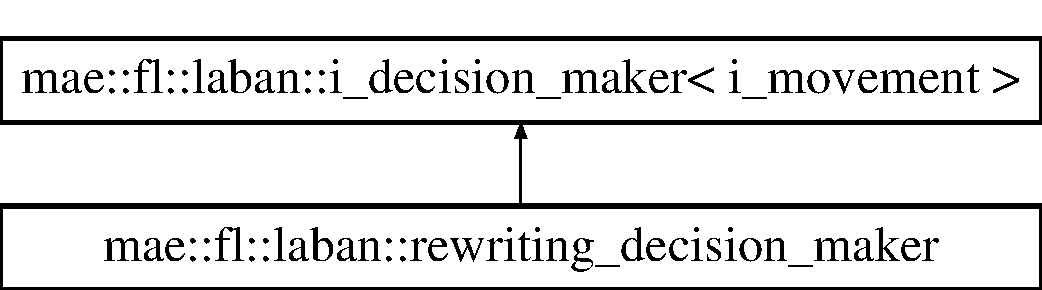
\includegraphics[height=2.000000cm]{classmae_1_1fl_1_1laban_1_1rewriting__decision__maker}
\end{center}
\end{figure}
\subsection*{Public Member Functions}
\begin{DoxyCompactItemize}
\item 
\hyperlink{classmae_1_1fl_1_1laban_1_1rewriting__decision__maker_af1d9dbfca7df3e5219641e3c5ef4c8d1}{rewriting\-\_\-decision\-\_\-maker} ()
\item 
virtual void \hyperlink{classmae_1_1fl_1_1laban_1_1rewriting__decision__maker_a2904cfea7637998087e5e387f077d9e9}{set\-\_\-recognition\-\_\-tolerance} (double tolerance)
\item 
virtual double \hyperlink{classmae_1_1fl_1_1laban_1_1rewriting__decision__maker_aa21cd4d1affba8c2e784565aee732456}{get\-\_\-recognition\-\_\-tolerance} ()
\item 
virtual bool \hyperlink{classmae_1_1fl_1_1laban_1_1rewriting__decision__maker_ae33a9f027e52bab0cc9be93eeb589d64}{decide\-\_\-match} (std\-::shared\-\_\-ptr$<$ \hyperlink{classmae_1_1fl_1_1laban_1_1i__movement}{i\-\_\-movement} $>$ stream\-\_\-item, std\-::shared\-\_\-ptr$<$ \hyperlink{classmae_1_1fl_1_1laban_1_1i__movement}{i\-\_\-movement} $>$ stream\-\_\-item\-\_\-predecessor, std\-::shared\-\_\-ptr$<$ \hyperlink{classmae_1_1fl_1_1laban_1_1i__movement}{i\-\_\-movement} $>$ tree\-\_\-item, std\-::shared\-\_\-ptr$<$ \hyperlink{classmae_1_1fl_1_1laban_1_1i__movement}{i\-\_\-movement} $>$ tree\-\_\-item\-\_\-predecessor)
\item 
virtual bool \hyperlink{classmae_1_1fl_1_1laban_1_1rewriting__decision__maker_a01849dbcdda4878338a3cda18f7040a8}{decide\-\_\-insertion} (std\-::shared\-\_\-ptr$<$ \hyperlink{classmae_1_1fl_1_1laban_1_1i__movement}{i\-\_\-movement} $>$ add\-\_\-item, std\-::shared\-\_\-ptr$<$ \hyperlink{classmae_1_1fl_1_1laban_1_1i__movement}{i\-\_\-movement} $>$ add\-\_\-item\-\_\-predecessor, std\-::shared\-\_\-ptr$<$ \hyperlink{classmae_1_1fl_1_1laban_1_1i__movement}{i\-\_\-movement} $>$ tree\-\_\-item, std\-::shared\-\_\-ptr$<$ \hyperlink{classmae_1_1fl_1_1laban_1_1i__movement}{i\-\_\-movement} $>$ tree\-\_\-item\-\_\-predecessor)
\item 
virtual bool \hyperlink{classmae_1_1fl_1_1laban_1_1rewriting__decision__maker_aee7c8ddde89262cc7a9c26ad041ea344}{position\-\_\-okay} (double dist\-\_\-to\-\_\-last, double set\-\_\-value, bool check\-\_\-startpose)
\end{DoxyCompactItemize}
\subsection*{Protected Member Functions}
\begin{DoxyCompactItemize}
\item 
virtual bool \hyperlink{classmae_1_1fl_1_1laban_1_1rewriting__decision__maker_a9cf4ad043611ae5bb95049e13cc4d184}{check\-\_\-type} (std\-::shared\-\_\-ptr$<$ \hyperlink{classmae_1_1fl_1_1laban_1_1i__movement}{i\-\_\-movement} $>$ a, std\-::shared\-\_\-ptr$<$ \hyperlink{classmae_1_1fl_1_1laban_1_1i__movement}{i\-\_\-movement} $>$ b)
\end{DoxyCompactItemize}


\subsection{Constructor \& Destructor Documentation}
\hypertarget{classmae_1_1fl_1_1laban_1_1rewriting__decision__maker_af1d9dbfca7df3e5219641e3c5ef4c8d1}{\index{mae\-::fl\-::laban\-::rewriting\-\_\-decision\-\_\-maker@{mae\-::fl\-::laban\-::rewriting\-\_\-decision\-\_\-maker}!rewriting\-\_\-decision\-\_\-maker@{rewriting\-\_\-decision\-\_\-maker}}
\index{rewriting\-\_\-decision\-\_\-maker@{rewriting\-\_\-decision\-\_\-maker}!mae::fl::laban::rewriting_decision_maker@{mae\-::fl\-::laban\-::rewriting\-\_\-decision\-\_\-maker}}
\subsubsection[{rewriting\-\_\-decision\-\_\-maker}]{\setlength{\rightskip}{0pt plus 5cm}mae\-::fl\-::laban\-::rewriting\-\_\-decision\-\_\-maker\-::rewriting\-\_\-decision\-\_\-maker (
\begin{DoxyParamCaption}
{}
\end{DoxyParamCaption}
)}}\label{classmae_1_1fl_1_1laban_1_1rewriting__decision__maker_af1d9dbfca7df3e5219641e3c5ef4c8d1}
Creates a new rewriting decision maker which is used to decide whether two movements are equal for sequences that are meant to be replaced. Therefore the timing does not matter but only the symbols. 

\subsection{Member Function Documentation}
\hypertarget{classmae_1_1fl_1_1laban_1_1rewriting__decision__maker_a9cf4ad043611ae5bb95049e13cc4d184}{\index{mae\-::fl\-::laban\-::rewriting\-\_\-decision\-\_\-maker@{mae\-::fl\-::laban\-::rewriting\-\_\-decision\-\_\-maker}!check\-\_\-type@{check\-\_\-type}}
\index{check\-\_\-type@{check\-\_\-type}!mae::fl::laban::rewriting_decision_maker@{mae\-::fl\-::laban\-::rewriting\-\_\-decision\-\_\-maker}}
\subsubsection[{check\-\_\-type}]{\setlength{\rightskip}{0pt plus 5cm}bool mae\-::fl\-::laban\-::rewriting\-\_\-decision\-\_\-maker\-::check\-\_\-type (
\begin{DoxyParamCaption}
\item[{std\-::shared\-\_\-ptr$<$ {\bf i\-\_\-movement} $>$}]{a, }
\item[{std\-::shared\-\_\-ptr$<$ {\bf i\-\_\-movement} $>$}]{b}
\end{DoxyParamCaption}
)\hspace{0.3cm}{\ttfamily [protected]}, {\ttfamily [virtual]}}}\label{classmae_1_1fl_1_1laban_1_1rewriting__decision__maker_a9cf4ad043611ae5bb95049e13cc4d184}
Checks whether the two movements are of the same type.


\begin{DoxyParams}{Parameters}
{\em a} & The first movement. \\
\hline
{\em b} & The second movement. \\
\hline
\end{DoxyParams}
\begin{DoxyReturn}{Returns}
True if matching. 
\end{DoxyReturn}
\hypertarget{classmae_1_1fl_1_1laban_1_1rewriting__decision__maker_a01849dbcdda4878338a3cda18f7040a8}{\index{mae\-::fl\-::laban\-::rewriting\-\_\-decision\-\_\-maker@{mae\-::fl\-::laban\-::rewriting\-\_\-decision\-\_\-maker}!decide\-\_\-insertion@{decide\-\_\-insertion}}
\index{decide\-\_\-insertion@{decide\-\_\-insertion}!mae::fl::laban::rewriting_decision_maker@{mae\-::fl\-::laban\-::rewriting\-\_\-decision\-\_\-maker}}
\subsubsection[{decide\-\_\-insertion}]{\setlength{\rightskip}{0pt plus 5cm}bool mae\-::fl\-::laban\-::rewriting\-\_\-decision\-\_\-maker\-::decide\-\_\-insertion (
\begin{DoxyParamCaption}
\item[{std\-::shared\-\_\-ptr$<$ {\bf i\-\_\-movement} $>$}]{add\-\_\-item, }
\item[{std\-::shared\-\_\-ptr$<$ {\bf i\-\_\-movement} $>$}]{add\-\_\-item\-\_\-predecessor, }
\item[{std\-::shared\-\_\-ptr$<$ {\bf i\-\_\-movement} $>$}]{tree\-\_\-item, }
\item[{std\-::shared\-\_\-ptr$<$ {\bf i\-\_\-movement} $>$}]{tree\-\_\-item\-\_\-predecessor}
\end{DoxyParamCaption}
)\hspace{0.3cm}{\ttfamily [virtual]}}}\label{classmae_1_1fl_1_1laban_1_1rewriting__decision__maker_a01849dbcdda4878338a3cda18f7040a8}
Checks whether the two elements match in order to provide the decision result for an insertion. Their predecessors are provided in order to make more complex decisions.


\begin{DoxyParams}{Parameters}
{\em stream\-\_\-item} & The element for the sequence to be added. \\
\hline
{\em stream\-\_\-item\-\_\-predecessor} & The predecessor element for the sequence to be added. \\
\hline
{\em tree\-\_\-item} & The decision tree's element. \\
\hline
{\em tree\-\_\-item\-\_\-predecessor} & The predecessor of the decision tree's element. \\
\hline
\end{DoxyParams}
\begin{DoxyReturn}{Returns}

\end{DoxyReturn}


Implements \hyperlink{classmae_1_1fl_1_1laban_1_1i__decision__maker_a728e6e706f54a6f8dfbeff9a267afbf4}{mae\-::fl\-::laban\-::i\-\_\-decision\-\_\-maker$<$ i\-\_\-movement $>$}.

\hypertarget{classmae_1_1fl_1_1laban_1_1rewriting__decision__maker_ae33a9f027e52bab0cc9be93eeb589d64}{\index{mae\-::fl\-::laban\-::rewriting\-\_\-decision\-\_\-maker@{mae\-::fl\-::laban\-::rewriting\-\_\-decision\-\_\-maker}!decide\-\_\-match@{decide\-\_\-match}}
\index{decide\-\_\-match@{decide\-\_\-match}!mae::fl::laban::rewriting_decision_maker@{mae\-::fl\-::laban\-::rewriting\-\_\-decision\-\_\-maker}}
\subsubsection[{decide\-\_\-match}]{\setlength{\rightskip}{0pt plus 5cm}bool mae\-::fl\-::laban\-::rewriting\-\_\-decision\-\_\-maker\-::decide\-\_\-match (
\begin{DoxyParamCaption}
\item[{std\-::shared\-\_\-ptr$<$ {\bf i\-\_\-movement} $>$}]{stream\-\_\-item, }
\item[{std\-::shared\-\_\-ptr$<$ {\bf i\-\_\-movement} $>$}]{stream\-\_\-item\-\_\-predecessor, }
\item[{std\-::shared\-\_\-ptr$<$ {\bf i\-\_\-movement} $>$}]{tree\-\_\-item, }
\item[{std\-::shared\-\_\-ptr$<$ {\bf i\-\_\-movement} $>$}]{tree\-\_\-item\-\_\-predecessor}
\end{DoxyParamCaption}
)\hspace{0.3cm}{\ttfamily [virtual]}}}\label{classmae_1_1fl_1_1laban_1_1rewriting__decision__maker_ae33a9f027e52bab0cc9be93eeb589d64}
Checks whether the two elements match in order to provide the decision result for a match. Their predecessors are provided in order to make more complex decisions.


\begin{DoxyParams}{Parameters}
{\em stream\-\_\-item} & The element for the sequence to be matched. \\
\hline
{\em stream\-\_\-item\-\_\-predecessor} & The predecessor element for the sequence to be matched. \\
\hline
{\em tree\-\_\-item} & The decision tree's element. \\
\hline
{\em tree\-\_\-item\-\_\-predecessor} & The predecessor of the decision tree's element. \\
\hline
\end{DoxyParams}
\begin{DoxyReturn}{Returns}
True if elements match. 
\end{DoxyReturn}


Implements \hyperlink{classmae_1_1fl_1_1laban_1_1i__decision__maker_ae1eb31ffcd38bcf0b207fee760ce98a6}{mae\-::fl\-::laban\-::i\-\_\-decision\-\_\-maker$<$ i\-\_\-movement $>$}.

\hypertarget{classmae_1_1fl_1_1laban_1_1rewriting__decision__maker_aa21cd4d1affba8c2e784565aee732456}{\index{mae\-::fl\-::laban\-::rewriting\-\_\-decision\-\_\-maker@{mae\-::fl\-::laban\-::rewriting\-\_\-decision\-\_\-maker}!get\-\_\-recognition\-\_\-tolerance@{get\-\_\-recognition\-\_\-tolerance}}
\index{get\-\_\-recognition\-\_\-tolerance@{get\-\_\-recognition\-\_\-tolerance}!mae::fl::laban::rewriting_decision_maker@{mae\-::fl\-::laban\-::rewriting\-\_\-decision\-\_\-maker}}
\subsubsection[{get\-\_\-recognition\-\_\-tolerance}]{\setlength{\rightskip}{0pt plus 5cm}double mae\-::fl\-::laban\-::rewriting\-\_\-decision\-\_\-maker\-::get\-\_\-recognition\-\_\-tolerance (
\begin{DoxyParamCaption}
{}
\end{DoxyParamCaption}
)\hspace{0.3cm}{\ttfamily [virtual]}}}\label{classmae_1_1fl_1_1laban_1_1rewriting__decision__maker_aa21cd4d1affba8c2e784565aee732456}
Returns the tolerance for the recognition. The tolerance is a value which represents the number of beats of the labanotation which are tolerated in deviation.

\begin{DoxyReturn}{Returns}
The tolerance. 
\end{DoxyReturn}


Implements \hyperlink{classmae_1_1fl_1_1laban_1_1i__decision__maker_aa892f42c6407b3f8c9a67b71993103ea}{mae\-::fl\-::laban\-::i\-\_\-decision\-\_\-maker$<$ i\-\_\-movement $>$}.

\hypertarget{classmae_1_1fl_1_1laban_1_1rewriting__decision__maker_aee7c8ddde89262cc7a9c26ad041ea344}{\index{mae\-::fl\-::laban\-::rewriting\-\_\-decision\-\_\-maker@{mae\-::fl\-::laban\-::rewriting\-\_\-decision\-\_\-maker}!position\-\_\-okay@{position\-\_\-okay}}
\index{position\-\_\-okay@{position\-\_\-okay}!mae::fl::laban::rewriting_decision_maker@{mae\-::fl\-::laban\-::rewriting\-\_\-decision\-\_\-maker}}
\subsubsection[{position\-\_\-okay}]{\setlength{\rightskip}{0pt plus 5cm}bool mae\-::fl\-::laban\-::rewriting\-\_\-decision\-\_\-maker\-::position\-\_\-okay (
\begin{DoxyParamCaption}
\item[{double}]{dist\-\_\-to\-\_\-last, }
\item[{double}]{set\-\_\-value, }
\item[{bool}]{check\-\_\-startpose}
\end{DoxyParamCaption}
)\hspace{0.3cm}{\ttfamily [virtual]}}}\label{classmae_1_1fl_1_1laban_1_1rewriting__decision__maker_aee7c8ddde89262cc7a9c26ad041ea344}
Checks the distances of the last element in this column to the last element of all columns. The method takes care of start poses on the set value side, so that only minimum distance must match and not an interval.


\begin{DoxyParams}{Parameters}
{\em dist\-\_\-to\-\_\-last} & The distance to the last element of all columns. \\
\hline
{\em set\-\_\-value} & The set value for the distance. \\
\hline
{\em check\-\_\-startpose} & True if set value is to start pose but dist is not. \\
\hline
\end{DoxyParams}
\begin{DoxyReturn}{Returns}
True if accepted. 
\end{DoxyReturn}


Implements \hyperlink{classmae_1_1fl_1_1laban_1_1i__decision__maker_aad9230ee447afc0d6cf70cd74c54cf41}{mae\-::fl\-::laban\-::i\-\_\-decision\-\_\-maker$<$ i\-\_\-movement $>$}.

\hypertarget{classmae_1_1fl_1_1laban_1_1rewriting__decision__maker_a2904cfea7637998087e5e387f077d9e9}{\index{mae\-::fl\-::laban\-::rewriting\-\_\-decision\-\_\-maker@{mae\-::fl\-::laban\-::rewriting\-\_\-decision\-\_\-maker}!set\-\_\-recognition\-\_\-tolerance@{set\-\_\-recognition\-\_\-tolerance}}
\index{set\-\_\-recognition\-\_\-tolerance@{set\-\_\-recognition\-\_\-tolerance}!mae::fl::laban::rewriting_decision_maker@{mae\-::fl\-::laban\-::rewriting\-\_\-decision\-\_\-maker}}
\subsubsection[{set\-\_\-recognition\-\_\-tolerance}]{\setlength{\rightskip}{0pt plus 5cm}void mae\-::fl\-::laban\-::rewriting\-\_\-decision\-\_\-maker\-::set\-\_\-recognition\-\_\-tolerance (
\begin{DoxyParamCaption}
\item[{double}]{tolerance}
\end{DoxyParamCaption}
)\hspace{0.3cm}{\ttfamily [virtual]}}}\label{classmae_1_1fl_1_1laban_1_1rewriting__decision__maker_a2904cfea7637998087e5e387f077d9e9}
Sets the tolerance for the recognition. The tolerance is a value which represents the number of beats of the labanotation which are tolerated in deviation.


\begin{DoxyParams}{Parameters}
{\em tolerance} & The tolerance to be accepted. \\
\hline
\end{DoxyParams}


Implements \hyperlink{classmae_1_1fl_1_1laban_1_1i__decision__maker_a63f05f6a3fb2a5f3b53f6555eada6243}{mae\-::fl\-::laban\-::i\-\_\-decision\-\_\-maker$<$ i\-\_\-movement $>$}.



The documentation for this class was generated from the following files\-:\begin{DoxyCompactItemize}
\item 
src/mae/fl/laban/rewriting\-\_\-decision\-\_\-maker.\-hpp\item 
src/mae/fl/laban/rewriting\-\_\-decision\-\_\-maker.\-cpp\end{DoxyCompactItemize}

\hypertarget{classmae_1_1fl_1_1laban_1_1rewriting__forest}{\section{mae\-:\-:fl\-:\-:laban\-:\-:rewriting\-\_\-forest Class Reference}
\label{classmae_1_1fl_1_1laban_1_1rewriting__forest}\index{mae\-::fl\-::laban\-::rewriting\-\_\-forest@{mae\-::fl\-::laban\-::rewriting\-\_\-forest}}
}
\subsection*{Public Member Functions}
\begin{DoxyCompactItemize}
\item 
\hyperlink{classmae_1_1fl_1_1laban_1_1rewriting__forest_a0eb4a90941ad2a400682a03e3abd136e}{rewriting\-\_\-forest} (unsigned int beats\-\_\-per\-\_\-measure=\hyperlink{classmae_1_1fl_1_1laban_1_1laban__sequence_a2e64362d5cfeb89eb8545cb064e63170}{laban\-\_\-sequence\-::default\-\_\-beats\-\_\-per\-\_\-measure}(), unsigned int beat\-\_\-duration=\hyperlink{classmae_1_1fl_1_1laban_1_1laban__sequence_ac7bf04cdac0c3aed6b8ee4a887e561d9}{laban\-\_\-sequence\-::default\-\_\-beat\-\_\-duration}(), e\-\_\-time\-\_\-unit time\-\_\-unit=\hyperlink{classmae_1_1fl_1_1laban_1_1laban__sequence_ada28215d43d85e983fe6129e9816eed2}{laban\-\_\-sequence\-::default\-\_\-time\-\_\-unit}(), double tolerance=0.\-5)
\item 
\hyperlink{classmae_1_1fl_1_1laban_1_1rewriting__forest_aa7d56018ed383a4d56d597761d5b8860}{rewriting\-\_\-forest} (std\-::vector$<$ std\-::shared\-\_\-ptr$<$ \hyperlink{classmae_1_1fl_1_1laban_1_1decision__value}{decision\-\_\-value}$<$ \hyperlink{classmae_1_1fl_1_1laban_1_1i__movement}{i\-\_\-movement}, std\-::vector$<$ std\-::vector$<$ std\-::shared\-\_\-ptr$<$ \hyperlink{classmae_1_1fl_1_1laban_1_1i__movement}{i\-\_\-movement} $>$ $>$ $>$ $>$ $>$ $>$ rules, unsigned int beats\-\_\-per\-\_\-measure=\hyperlink{classmae_1_1fl_1_1laban_1_1laban__sequence_a2e64362d5cfeb89eb8545cb064e63170}{laban\-\_\-sequence\-::default\-\_\-beats\-\_\-per\-\_\-measure}(), unsigned int beat\-\_\-duration=\hyperlink{classmae_1_1fl_1_1laban_1_1laban__sequence_ac7bf04cdac0c3aed6b8ee4a887e561d9}{laban\-\_\-sequence\-::default\-\_\-beat\-\_\-duration}(), e\-\_\-time\-\_\-unit time\-\_\-unit=\hyperlink{classmae_1_1fl_1_1laban_1_1laban__sequence_ada28215d43d85e983fe6129e9816eed2}{laban\-\_\-sequence\-::default\-\_\-time\-\_\-unit}(), double tolerance=0.\-5)
\item 
virtual double \hyperlink{classmae_1_1fl_1_1laban_1_1rewriting__forest_ac919e5e07a781165e39a710d27346b1c}{get\-\_\-tolerance} ()
\item 
virtual void \hyperlink{classmae_1_1fl_1_1laban_1_1rewriting__forest_a2e1d1eb1d939024e61db33dbbb9d85b0}{set\-\_\-tolerance} (double tolerance)
\item 
virtual std\-::vector\\*
$<$ std\-::vector$<$ std\-::shared\-\_\-ptr\\*
$<$ \hyperlink{classmae_1_1fl_1_1laban_1_1i__movement}{i\-\_\-movement} $>$ $>$ $>$ \hyperlink{classmae_1_1fl_1_1laban_1_1rewriting__forest_a1af307de2c89df6c63738a51ce0f4f54}{replacements} (std\-::vector$<$ std\-::shared\-\_\-ptr$<$ \hyperlink{classmae_1_1fl_1_1laban_1_1i__movement}{i\-\_\-movement} $>$ $>$ sequence)
\item 
virtual void \hyperlink{classmae_1_1fl_1_1laban_1_1rewriting__forest_aa9859191a391f3984ba58c60bc034c65}{add\-\_\-rule} (std\-::vector$<$ std\-::shared\-\_\-ptr$<$ \hyperlink{classmae_1_1fl_1_1laban_1_1i__movement}{i\-\_\-movement} $>$ $>$ sequence, std\-::shared\-\_\-ptr$<$ std\-::vector$<$ std\-::vector$<$ std\-::shared\-\_\-ptr$<$ \hyperlink{classmae_1_1fl_1_1laban_1_1i__movement}{i\-\_\-movement} $>$ $>$ $>$ $>$ \hyperlink{classmae_1_1fl_1_1laban_1_1rewriting__forest_a1af307de2c89df6c63738a51ce0f4f54}{replacements})
\item 
virtual void \hyperlink{classmae_1_1fl_1_1laban_1_1rewriting__forest_a04afb631b9d710c3e591bcca716e353e}{add\-\_\-rule} (std\-::shared\-\_\-ptr$<$ \hyperlink{classmae_1_1fl_1_1laban_1_1decision__value}{decision\-\_\-value}$<$ \hyperlink{classmae_1_1fl_1_1laban_1_1i__movement}{i\-\_\-movement}, std\-::vector$<$ std\-::vector$<$ std\-::shared\-\_\-ptr$<$ \hyperlink{classmae_1_1fl_1_1laban_1_1i__movement}{i\-\_\-movement} $>$ $>$ $>$ $>$ $>$ rule)
\item 
virtual std\-::string \hyperlink{classmae_1_1fl_1_1laban_1_1rewriting__forest_ab096895fc65e8dc3af344228c1ddd70a}{str} ()
\end{DoxyCompactItemize}


\subsection{Constructor \& Destructor Documentation}
\hypertarget{classmae_1_1fl_1_1laban_1_1rewriting__forest_a0eb4a90941ad2a400682a03e3abd136e}{\index{mae\-::fl\-::laban\-::rewriting\-\_\-forest@{mae\-::fl\-::laban\-::rewriting\-\_\-forest}!rewriting\-\_\-forest@{rewriting\-\_\-forest}}
\index{rewriting\-\_\-forest@{rewriting\-\_\-forest}!mae::fl::laban::rewriting_forest@{mae\-::fl\-::laban\-::rewriting\-\_\-forest}}
\subsubsection[{rewriting\-\_\-forest}]{\setlength{\rightskip}{0pt plus 5cm}mae\-::fl\-::laban\-::rewriting\-\_\-forest\-::rewriting\-\_\-forest (
\begin{DoxyParamCaption}
\item[{unsigned int}]{beats\-\_\-per\-\_\-measure = {\ttfamily {\bf laban\-\_\-sequence\-::default\-\_\-beats\-\_\-per\-\_\-measure}()}, }
\item[{unsigned int}]{beat\-\_\-duration = {\ttfamily {\bf laban\-\_\-sequence\-::default\-\_\-beat\-\_\-duration}()}, }
\item[{e\-\_\-time\-\_\-unit}]{time\-\_\-unit = {\ttfamily {\bf laban\-\_\-sequence\-::default\-\_\-time\-\_\-unit}()}, }
\item[{double}]{tolerance = {\ttfamily 0.5}}
\end{DoxyParamCaption}
)}}\label{classmae_1_1fl_1_1laban_1_1rewriting__forest_a0eb4a90941ad2a400682a03e3abd136e}
Creates a new decision forest for rewriting rules.


\begin{DoxyParams}{Parameters}
{\em beats\-\_\-per\-\_\-measure} & The beats per measure as used by the laban sequence generator. \\
\hline
{\em beat\-\_\-duration} & The beat duration as used by the laban sequence generator. \\
\hline
{\em time\-\_\-unit} & The time unit as used by the laban sequence generator. \\
\hline
\end{DoxyParams}
\hypertarget{classmae_1_1fl_1_1laban_1_1rewriting__forest_aa7d56018ed383a4d56d597761d5b8860}{\index{mae\-::fl\-::laban\-::rewriting\-\_\-forest@{mae\-::fl\-::laban\-::rewriting\-\_\-forest}!rewriting\-\_\-forest@{rewriting\-\_\-forest}}
\index{rewriting\-\_\-forest@{rewriting\-\_\-forest}!mae::fl::laban::rewriting_forest@{mae\-::fl\-::laban\-::rewriting\-\_\-forest}}
\subsubsection[{rewriting\-\_\-forest}]{\setlength{\rightskip}{0pt plus 5cm}mae\-::fl\-::laban\-::rewriting\-\_\-forest\-::rewriting\-\_\-forest (
\begin{DoxyParamCaption}
\item[{std\-::vector$<$ std\-::shared\-\_\-ptr$<$ {\bf decision\-\_\-value}$<$ {\bf i\-\_\-movement}, std\-::vector$<$ std\-::vector$<$ std\-::shared\-\_\-ptr$<$ {\bf i\-\_\-movement} $>$ $>$ $>$ $>$ $>$ $>$}]{rules, }
\item[{unsigned int}]{beats\-\_\-per\-\_\-measure = {\ttfamily {\bf laban\-\_\-sequence\-::default\-\_\-beats\-\_\-per\-\_\-measure}()}, }
\item[{unsigned int}]{beat\-\_\-duration = {\ttfamily {\bf laban\-\_\-sequence\-::default\-\_\-beat\-\_\-duration}()}, }
\item[{e\-\_\-time\-\_\-unit}]{time\-\_\-unit = {\ttfamily {\bf laban\-\_\-sequence\-::default\-\_\-time\-\_\-unit}()}, }
\item[{double}]{tolerance = {\ttfamily 0.5}}
\end{DoxyParamCaption}
)}}\label{classmae_1_1fl_1_1laban_1_1rewriting__forest_aa7d56018ed383a4d56d597761d5b8860}
Creates a new decision forest for rewriting rules with initial rules set.


\begin{DoxyParams}{Parameters}
{\em rules} & The rules to be added to the forest. \\
\hline
{\em beats\-\_\-per\-\_\-measure} & The beats per measure as used by the laban sequence generator. \\
\hline
{\em beat\-\_\-duration} & The beat duration as used by the laban sequence generator. \\
\hline
{\em time\-\_\-unit} & The time unit as used by the laban sequence generator. \\
\hline
{\em tolerance} & The tolerance applied for finding continuous movements. \\
\hline
\end{DoxyParams}


\subsection{Member Function Documentation}
\hypertarget{classmae_1_1fl_1_1laban_1_1rewriting__forest_aa9859191a391f3984ba58c60bc034c65}{\index{mae\-::fl\-::laban\-::rewriting\-\_\-forest@{mae\-::fl\-::laban\-::rewriting\-\_\-forest}!add\-\_\-rule@{add\-\_\-rule}}
\index{add\-\_\-rule@{add\-\_\-rule}!mae::fl::laban::rewriting_forest@{mae\-::fl\-::laban\-::rewriting\-\_\-forest}}
\subsubsection[{add\-\_\-rule}]{\setlength{\rightskip}{0pt plus 5cm}void mae\-::fl\-::laban\-::rewriting\-\_\-forest\-::add\-\_\-rule (
\begin{DoxyParamCaption}
\item[{std\-::vector$<$ std\-::shared\-\_\-ptr$<$ {\bf i\-\_\-movement} $>$ $>$}]{sequence, }
\item[{std\-::shared\-\_\-ptr$<$ std\-::vector$<$ std\-::vector$<$ std\-::shared\-\_\-ptr$<$ {\bf i\-\_\-movement} $>$ $>$ $>$ $>$}]{replacements}
\end{DoxyParamCaption}
)\hspace{0.3cm}{\ttfamily [virtual]}}}\label{classmae_1_1fl_1_1laban_1_1rewriting__forest_aa9859191a391f3984ba58c60bc034c65}
Adds a rewriting rule to the forest.


\begin{DoxyParams}{Parameters}
{\em sequence} & The sequence. \\
\hline
{\em replacements} & The replacement for the sequence. \\
\hline
\end{DoxyParams}
\hypertarget{classmae_1_1fl_1_1laban_1_1rewriting__forest_a04afb631b9d710c3e591bcca716e353e}{\index{mae\-::fl\-::laban\-::rewriting\-\_\-forest@{mae\-::fl\-::laban\-::rewriting\-\_\-forest}!add\-\_\-rule@{add\-\_\-rule}}
\index{add\-\_\-rule@{add\-\_\-rule}!mae::fl::laban::rewriting_forest@{mae\-::fl\-::laban\-::rewriting\-\_\-forest}}
\subsubsection[{add\-\_\-rule}]{\setlength{\rightskip}{0pt plus 5cm}void mae\-::fl\-::laban\-::rewriting\-\_\-forest\-::add\-\_\-rule (
\begin{DoxyParamCaption}
\item[{std\-::shared\-\_\-ptr$<$ {\bf decision\-\_\-value}$<$ {\bf i\-\_\-movement}, std\-::vector$<$ std\-::vector$<$ std\-::shared\-\_\-ptr$<$ {\bf i\-\_\-movement} $>$ $>$ $>$ $>$ $>$}]{rule}
\end{DoxyParamCaption}
)\hspace{0.3cm}{\ttfamily [virtual]}}}\label{classmae_1_1fl_1_1laban_1_1rewriting__forest_a04afb631b9d710c3e591bcca716e353e}
Adds a rewriting rule to the forest.


\begin{DoxyParams}{Parameters}
{\em rule} & The rule to be added. \\
\hline
\end{DoxyParams}
\hypertarget{classmae_1_1fl_1_1laban_1_1rewriting__forest_ac919e5e07a781165e39a710d27346b1c}{\index{mae\-::fl\-::laban\-::rewriting\-\_\-forest@{mae\-::fl\-::laban\-::rewriting\-\_\-forest}!get\-\_\-tolerance@{get\-\_\-tolerance}}
\index{get\-\_\-tolerance@{get\-\_\-tolerance}!mae::fl::laban::rewriting_forest@{mae\-::fl\-::laban\-::rewriting\-\_\-forest}}
\subsubsection[{get\-\_\-tolerance}]{\setlength{\rightskip}{0pt plus 5cm}double mae\-::fl\-::laban\-::rewriting\-\_\-forest\-::get\-\_\-tolerance (
\begin{DoxyParamCaption}
{}
\end{DoxyParamCaption}
)\hspace{0.3cm}{\ttfamily [virtual]}}}\label{classmae_1_1fl_1_1laban_1_1rewriting__forest_ac919e5e07a781165e39a710d27346b1c}
Returns the tolerance value (in beats) for a connected sequence.

\begin{DoxyReturn}{Returns}
The tolerance. 
\end{DoxyReturn}
\hypertarget{classmae_1_1fl_1_1laban_1_1rewriting__forest_a1af307de2c89df6c63738a51ce0f4f54}{\index{mae\-::fl\-::laban\-::rewriting\-\_\-forest@{mae\-::fl\-::laban\-::rewriting\-\_\-forest}!replacements@{replacements}}
\index{replacements@{replacements}!mae::fl::laban::rewriting_forest@{mae\-::fl\-::laban\-::rewriting\-\_\-forest}}
\subsubsection[{replacements}]{\setlength{\rightskip}{0pt plus 5cm}std\-::vector$<$ std\-::vector$<$ std\-::shared\-\_\-ptr$<$ {\bf i\-\_\-movement} $>$ $>$ $>$ mae\-::fl\-::laban\-::rewriting\-\_\-forest\-::replacements (
\begin{DoxyParamCaption}
\item[{std\-::vector$<$ std\-::shared\-\_\-ptr$<$ {\bf i\-\_\-movement} $>$ $>$}]{sequence}
\end{DoxyParamCaption}
)\hspace{0.3cm}{\ttfamily [virtual]}}}\label{classmae_1_1fl_1_1laban_1_1rewriting__forest_a1af307de2c89df6c63738a51ce0f4f54}
Returns all equivalent sequences for the given sequence (this includes the unchanged sequence itself).


\begin{DoxyParams}{Parameters}
{\em sequence} & The sequence to be checked for replacements. \\
\hline
\end{DoxyParams}
\begin{DoxyReturn}{Returns}
All equivalent sequences. 
\end{DoxyReturn}
\hypertarget{classmae_1_1fl_1_1laban_1_1rewriting__forest_a2e1d1eb1d939024e61db33dbbb9d85b0}{\index{mae\-::fl\-::laban\-::rewriting\-\_\-forest@{mae\-::fl\-::laban\-::rewriting\-\_\-forest}!set\-\_\-tolerance@{set\-\_\-tolerance}}
\index{set\-\_\-tolerance@{set\-\_\-tolerance}!mae::fl::laban::rewriting_forest@{mae\-::fl\-::laban\-::rewriting\-\_\-forest}}
\subsubsection[{set\-\_\-tolerance}]{\setlength{\rightskip}{0pt plus 5cm}void mae\-::fl\-::laban\-::rewriting\-\_\-forest\-::set\-\_\-tolerance (
\begin{DoxyParamCaption}
\item[{double}]{tolerance}
\end{DoxyParamCaption}
)\hspace{0.3cm}{\ttfamily [virtual]}}}\label{classmae_1_1fl_1_1laban_1_1rewriting__forest_a2e1d1eb1d939024e61db33dbbb9d85b0}
Sets the tolerance value (in beats) for a connected sequence.


\begin{DoxyParams}{Parameters}
{\em tolerance} & The tolerance. \\
\hline
\end{DoxyParams}
\hypertarget{classmae_1_1fl_1_1laban_1_1rewriting__forest_ab096895fc65e8dc3af344228c1ddd70a}{\index{mae\-::fl\-::laban\-::rewriting\-\_\-forest@{mae\-::fl\-::laban\-::rewriting\-\_\-forest}!str@{str}}
\index{str@{str}!mae::fl::laban::rewriting_forest@{mae\-::fl\-::laban\-::rewriting\-\_\-forest}}
\subsubsection[{str}]{\setlength{\rightskip}{0pt plus 5cm}std\-::string mae\-::fl\-::laban\-::rewriting\-\_\-forest\-::str (
\begin{DoxyParamCaption}
{}
\end{DoxyParamCaption}
)\hspace{0.3cm}{\ttfamily [virtual]}}}\label{classmae_1_1fl_1_1laban_1_1rewriting__forest_ab096895fc65e8dc3af344228c1ddd70a}
Returns the string representation for the rewriting forest.

\begin{DoxyReturn}{Returns}
The string representation. 
\end{DoxyReturn}


The documentation for this class was generated from the following files\-:\begin{DoxyCompactItemize}
\item 
src/mae/fl/laban/rewriting\-\_\-forest.\-hpp\item 
src/mae/fl/laban/rewriting\-\_\-forest.\-cpp\end{DoxyCompactItemize}

\hypertarget{classmae_1_1fl_1_1laban_1_1rewriting__rules__reader}{\section{mae\-:\-:fl\-:\-:laban\-:\-:rewriting\-\_\-rules\-\_\-reader Class Reference}
\label{classmae_1_1fl_1_1laban_1_1rewriting__rules__reader}\index{mae\-::fl\-::laban\-::rewriting\-\_\-rules\-\_\-reader@{mae\-::fl\-::laban\-::rewriting\-\_\-rules\-\_\-reader}}
}
\subsection*{Public Member Functions}
\begin{DoxyCompactItemize}
\item 
\hyperlink{classmae_1_1fl_1_1laban_1_1rewriting__rules__reader_afca7b7ea63a56ba6f48d586a3c5f360e}{rewriting\-\_\-rules\-\_\-reader} ()
\item 
virtual std\-::vector\\*
$<$ std\-::shared\-\_\-ptr\\*
$<$ \hyperlink{classmae_1_1fl_1_1laban_1_1decision__value}{decision\-\_\-value}$<$ \hyperlink{classmae_1_1fl_1_1laban_1_1i__movement}{i\-\_\-movement}, \\*
std\-::vector$<$ std\-::vector\\*
$<$ std\-::shared\-\_\-ptr$<$ \hyperlink{classmae_1_1fl_1_1laban_1_1i__movement}{i\-\_\-movement} $>$ $>$ $>$ $>$ $>$ $>$ \hyperlink{classmae_1_1fl_1_1laban_1_1rewriting__rules__reader_ac6c2ccb66ebbf3b52b313a014e8ac642}{read\-\_\-rules\-\_\-file} (std\-::string file\-\_\-name)
\item 
virtual std\-::vector\\*
$<$ std\-::shared\-\_\-ptr\\*
$<$ \hyperlink{classmae_1_1fl_1_1laban_1_1decision__value}{decision\-\_\-value}$<$ \hyperlink{classmae_1_1fl_1_1laban_1_1i__movement}{i\-\_\-movement}, \\*
std\-::vector$<$ std\-::vector\\*
$<$ std\-::shared\-\_\-ptr$<$ \hyperlink{classmae_1_1fl_1_1laban_1_1i__movement}{i\-\_\-movement} $>$ $>$ $>$ $>$ $>$ $>$ \hyperlink{classmae_1_1fl_1_1laban_1_1rewriting__rules__reader_a60f1b64794dee467385b8d6bb9a69f99}{read\-\_\-rules\-\_\-str} (std\-::string xml\-\_\-string)
\end{DoxyCompactItemize}


\subsection{Constructor \& Destructor Documentation}
\hypertarget{classmae_1_1fl_1_1laban_1_1rewriting__rules__reader_afca7b7ea63a56ba6f48d586a3c5f360e}{\index{mae\-::fl\-::laban\-::rewriting\-\_\-rules\-\_\-reader@{mae\-::fl\-::laban\-::rewriting\-\_\-rules\-\_\-reader}!rewriting\-\_\-rules\-\_\-reader@{rewriting\-\_\-rules\-\_\-reader}}
\index{rewriting\-\_\-rules\-\_\-reader@{rewriting\-\_\-rules\-\_\-reader}!mae::fl::laban::rewriting_rules_reader@{mae\-::fl\-::laban\-::rewriting\-\_\-rules\-\_\-reader}}
\subsubsection[{rewriting\-\_\-rules\-\_\-reader}]{\setlength{\rightskip}{0pt plus 5cm}mae\-::fl\-::laban\-::rewriting\-\_\-rules\-\_\-reader\-::rewriting\-\_\-rules\-\_\-reader (
\begin{DoxyParamCaption}
{}
\end{DoxyParamCaption}
)}}\label{classmae_1_1fl_1_1laban_1_1rewriting__rules__reader_afca7b7ea63a56ba6f48d586a3c5f360e}
Creates a new reader for rewriting rules. 

\subsection{Member Function Documentation}
\hypertarget{classmae_1_1fl_1_1laban_1_1rewriting__rules__reader_ac6c2ccb66ebbf3b52b313a014e8ac642}{\index{mae\-::fl\-::laban\-::rewriting\-\_\-rules\-\_\-reader@{mae\-::fl\-::laban\-::rewriting\-\_\-rules\-\_\-reader}!read\-\_\-rules\-\_\-file@{read\-\_\-rules\-\_\-file}}
\index{read\-\_\-rules\-\_\-file@{read\-\_\-rules\-\_\-file}!mae::fl::laban::rewriting_rules_reader@{mae\-::fl\-::laban\-::rewriting\-\_\-rules\-\_\-reader}}
\subsubsection[{read\-\_\-rules\-\_\-file}]{\setlength{\rightskip}{0pt plus 5cm}std\-::vector$<$ std\-::shared\-\_\-ptr$<$ {\bf decision\-\_\-value}$<$ {\bf i\-\_\-movement}, std\-::vector$<$ std\-::vector$<$ std\-::shared\-\_\-ptr$<$ {\bf i\-\_\-movement} $>$ $>$ $>$ $>$ $>$ $>$ mae\-::fl\-::laban\-::rewriting\-\_\-rules\-\_\-reader\-::read\-\_\-rules\-\_\-file (
\begin{DoxyParamCaption}
\item[{std\-::string}]{file\-\_\-name}
\end{DoxyParamCaption}
)\hspace{0.3cm}{\ttfamily [virtual]}}}\label{classmae_1_1fl_1_1laban_1_1rewriting__rules__reader_ac6c2ccb66ebbf3b52b313a014e8ac642}
Reads the rewriting rules X\-M\-L file and generates a vector of rules from it.


\begin{DoxyParams}{Parameters}
{\em xml\-\_\-string} & The path to the X\-M\-L file. \\
\hline
\end{DoxyParams}
\begin{DoxyReturn}{Returns}
A shared pointer to the sequence. 
\end{DoxyReturn}
\hypertarget{classmae_1_1fl_1_1laban_1_1rewriting__rules__reader_a60f1b64794dee467385b8d6bb9a69f99}{\index{mae\-::fl\-::laban\-::rewriting\-\_\-rules\-\_\-reader@{mae\-::fl\-::laban\-::rewriting\-\_\-rules\-\_\-reader}!read\-\_\-rules\-\_\-str@{read\-\_\-rules\-\_\-str}}
\index{read\-\_\-rules\-\_\-str@{read\-\_\-rules\-\_\-str}!mae::fl::laban::rewriting_rules_reader@{mae\-::fl\-::laban\-::rewriting\-\_\-rules\-\_\-reader}}
\subsubsection[{read\-\_\-rules\-\_\-str}]{\setlength{\rightskip}{0pt plus 5cm}std\-::vector$<$ std\-::shared\-\_\-ptr$<$ {\bf decision\-\_\-value}$<$ {\bf i\-\_\-movement}, std\-::vector$<$ std\-::vector$<$ std\-::shared\-\_\-ptr$<$ {\bf i\-\_\-movement} $>$ $>$ $>$ $>$ $>$ $>$ mae\-::fl\-::laban\-::rewriting\-\_\-rules\-\_\-reader\-::read\-\_\-rules\-\_\-str (
\begin{DoxyParamCaption}
\item[{std\-::string}]{xml\-\_\-string}
\end{DoxyParamCaption}
)\hspace{0.3cm}{\ttfamily [virtual]}}}\label{classmae_1_1fl_1_1laban_1_1rewriting__rules__reader_a60f1b64794dee467385b8d6bb9a69f99}
Reads the rewriting rules X\-M\-L string and generates a vector of rules from it.


\begin{DoxyParams}{Parameters}
{\em xml\-\_\-string} & The X\-M\-L string. \\
\hline
\end{DoxyParams}
\begin{DoxyReturn}{Returns}
A shared pointer to the sequence. 
\end{DoxyReturn}


The documentation for this class was generated from the following files\-:\begin{DoxyCompactItemize}
\item 
src/mae/fl/laban/rewriting\-\_\-rules\-\_\-reader.\-hpp\item 
src/mae/fl/laban/rewriting\-\_\-rules\-\_\-reader.\-cpp\end{DoxyCompactItemize}

\hypertarget{classmae_1_1fl_1_1laban_1_1room__direction}{\section{mae\-:\-:fl\-:\-:laban\-:\-:room\-\_\-direction Class Reference}
\label{classmae_1_1fl_1_1laban_1_1room__direction}\index{mae\-::fl\-::laban\-::room\-\_\-direction@{mae\-::fl\-::laban\-::room\-\_\-direction}}
}
Inheritance diagram for mae\-:\-:fl\-:\-:laban\-:\-:room\-\_\-direction\-:\begin{figure}[H]
\begin{center}
\leavevmode
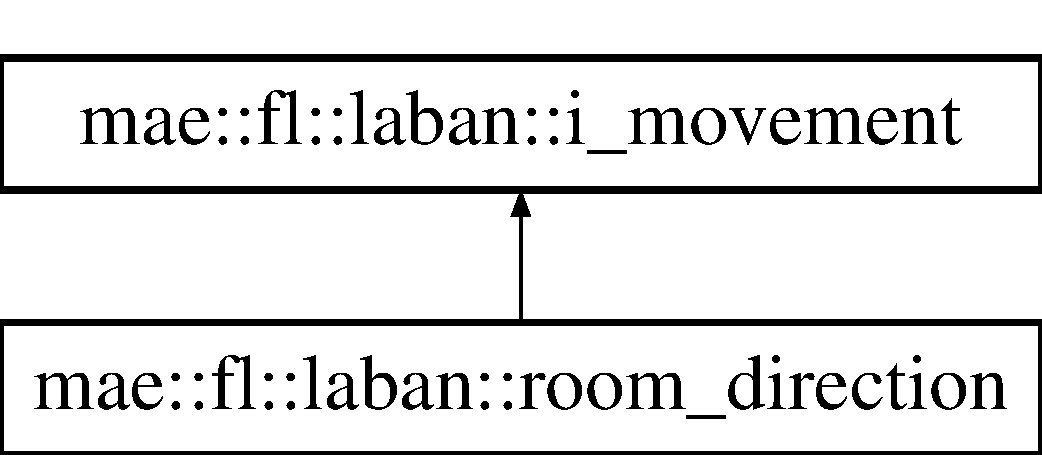
\includegraphics[height=2.000000cm]{classmae_1_1fl_1_1laban_1_1room__direction}
\end{center}
\end{figure}
\subsection*{Public Member Functions}
\begin{DoxyCompactItemize}
\item 
\hyperlink{classmae_1_1fl_1_1laban_1_1room__direction_af0df3de300b09be34d581a0a06256b1a}{room\-\_\-direction} (unsigned int measure, double beat, std\-::shared\-\_\-ptr$<$ \hyperlink{classmae_1_1fl_1_1laban_1_1mv_1_1pin}{mv\-::pin} $>$ direction)
\item 
virtual int \hyperlink{classmae_1_1fl_1_1laban_1_1room__direction_afa452f53f560485183e322571c9d1931}{get\-\_\-column} () const 
\item 
virtual unsigned int \hyperlink{classmae_1_1fl_1_1laban_1_1room__direction_aa7bf06d719e66f990debba5c1cc22f90}{get\-\_\-measure} () const 
\item 
virtual double \hyperlink{classmae_1_1fl_1_1laban_1_1room__direction_ad1b05ee39b84fc937170b2ef90af6f71}{get\-\_\-beat} () const 
\item 
virtual double \hyperlink{classmae_1_1fl_1_1laban_1_1room__direction_ae7cd8ee096a4cf46acfeba78a922c0cf}{get\-\_\-duration} () const 
\item 
std\-::shared\-\_\-ptr$<$ \hyperlink{classmae_1_1fl_1_1laban_1_1mv_1_1pin}{mv\-::pin} $>$ \hyperlink{classmae_1_1fl_1_1laban_1_1room__direction_a2a0ab5a17650a565c77c3f8f4ce70110}{get\-\_\-direction} () const 
\item 
virtual bool \hyperlink{classmae_1_1fl_1_1laban_1_1room__direction_a87704a471c16270f08a1b9f9ded7618d}{equals} (std\-::shared\-\_\-ptr$<$ \hyperlink{classmae_1_1fl_1_1laban_1_1i__movement}{i\-\_\-movement} $>$ a) const 
\item 
virtual bool \hyperlink{classmae_1_1fl_1_1laban_1_1room__direction_a0d3baa55c0408bc8c2386b2adfa53749}{symbol\-\_\-equals} (std\-::shared\-\_\-ptr$<$ \hyperlink{classmae_1_1fl_1_1laban_1_1i__movement}{i\-\_\-movement} $>$ a) const 
\item 
virtual std\-::string \hyperlink{classmae_1_1fl_1_1laban_1_1room__direction_a0d1a929061476676ca646dd5ff0d7ae8}{xml} (unsigned int indent=0, std\-::string namesp=\char`\"{}\char`\"{}) const 
\item 
virtual std\-::string \hyperlink{classmae_1_1fl_1_1laban_1_1room__direction_af7907869572c5927f02f49b3a7333b05}{svg} (unsigned int im\-\_\-width, unsigned int im\-\_\-height, unsigned int max\-\_\-column, unsigned int measures, unsigned int beats\-\_\-per\-\_\-measure) const 
\item 
virtual std\-::shared\-\_\-ptr\\*
$<$ \hyperlink{classmae_1_1fl_1_1laban_1_1i__movement}{i\-\_\-movement} $>$ \hyperlink{classmae_1_1fl_1_1laban_1_1room__direction_a776243cb6da19b5c0fe46c838c82002b}{recreate} (std\-::map$<$ int, int $>$ column\-\_\-mapping, unsigned int measure, double beat, double duration) const 
\item 
virtual std\-::string \hyperlink{classmae_1_1fl_1_1laban_1_1room__direction_ab8e8d61eb51db3da6a21cb2da455d307}{str} () const 
\end{DoxyCompactItemize}
\subsection*{Friends}
\begin{DoxyCompactItemize}
\item 
\hypertarget{classmae_1_1fl_1_1laban_1_1room__direction_a20bff2a9c40a4b06e423bb5a0c56cb6b}{std\-::ostream \& {\bfseries operator$<$$<$} (std\-::ostream \&os, const \hyperlink{classmae_1_1fl_1_1laban_1_1room__direction}{room\-\_\-direction} \&obj)}\label{classmae_1_1fl_1_1laban_1_1room__direction_a20bff2a9c40a4b06e423bb5a0c56cb6b}

\item 
\hypertarget{classmae_1_1fl_1_1laban_1_1room__direction_add5cd0cee6d75b43faad9eb83b689433}{std\-::ostream \& {\bfseries operator$<$$<$} (std\-::ostream \&os, const std\-::shared\-\_\-ptr$<$ \hyperlink{classmae_1_1fl_1_1laban_1_1room__direction}{room\-\_\-direction} $>$ \&obj)}\label{classmae_1_1fl_1_1laban_1_1room__direction_add5cd0cee6d75b43faad9eb83b689433}

\end{DoxyCompactItemize}


\subsection{Constructor \& Destructor Documentation}
\hypertarget{classmae_1_1fl_1_1laban_1_1room__direction_af0df3de300b09be34d581a0a06256b1a}{\index{mae\-::fl\-::laban\-::room\-\_\-direction@{mae\-::fl\-::laban\-::room\-\_\-direction}!room\-\_\-direction@{room\-\_\-direction}}
\index{room\-\_\-direction@{room\-\_\-direction}!mae::fl::laban::room_direction@{mae\-::fl\-::laban\-::room\-\_\-direction}}
\subsubsection[{room\-\_\-direction}]{\setlength{\rightskip}{0pt plus 5cm}mae\-::fl\-::laban\-::room\-\_\-direction\-::room\-\_\-direction (
\begin{DoxyParamCaption}
\item[{unsigned int}]{measure, }
\item[{double}]{beat, }
\item[{std\-::shared\-\_\-ptr$<$ {\bf mv\-::pin} $>$}]{direction}
\end{DoxyParamCaption}
)}}\label{classmae_1_1fl_1_1laban_1_1room__direction_af0df3de300b09be34d581a0a06256b1a}
Creates a room direction sign.


\begin{DoxyParams}{Parameters}
{\em measure} & The measure in which this symbol is placed. \\
\hline
{\em beat} & The beat where this symbol is placed. \\
\hline
{\em direction} & The direction of the room. \\
\hline
\end{DoxyParams}


\subsection{Member Function Documentation}
\hypertarget{classmae_1_1fl_1_1laban_1_1room__direction_a87704a471c16270f08a1b9f9ded7618d}{\index{mae\-::fl\-::laban\-::room\-\_\-direction@{mae\-::fl\-::laban\-::room\-\_\-direction}!equals@{equals}}
\index{equals@{equals}!mae::fl::laban::room_direction@{mae\-::fl\-::laban\-::room\-\_\-direction}}
\subsubsection[{equals}]{\setlength{\rightskip}{0pt plus 5cm}bool mae\-::fl\-::laban\-::room\-\_\-direction\-::equals (
\begin{DoxyParamCaption}
\item[{std\-::shared\-\_\-ptr$<$ {\bf i\-\_\-movement} $>$}]{a}
\end{DoxyParamCaption}
) const\hspace{0.3cm}{\ttfamily [virtual]}}}\label{classmae_1_1fl_1_1laban_1_1room__direction_a87704a471c16270f08a1b9f9ded7618d}
Returns true if the \hyperlink{classmae_1_1fl_1_1laban_1_1i__movement}{i\-\_\-movement} elements are equal.


\begin{DoxyParams}{Parameters}
{\em a} & The movement to be compared to. \\
\hline
\end{DoxyParams}
\begin{DoxyReturn}{Returns}
True if equal. 
\end{DoxyReturn}


Implements \hyperlink{classmae_1_1fl_1_1laban_1_1i__movement_a29783771372283ff2cc7deded01b83b1}{mae\-::fl\-::laban\-::i\-\_\-movement}.

\hypertarget{classmae_1_1fl_1_1laban_1_1room__direction_ad1b05ee39b84fc937170b2ef90af6f71}{\index{mae\-::fl\-::laban\-::room\-\_\-direction@{mae\-::fl\-::laban\-::room\-\_\-direction}!get\-\_\-beat@{get\-\_\-beat}}
\index{get\-\_\-beat@{get\-\_\-beat}!mae::fl::laban::room_direction@{mae\-::fl\-::laban\-::room\-\_\-direction}}
\subsubsection[{get\-\_\-beat}]{\setlength{\rightskip}{0pt plus 5cm}double mae\-::fl\-::laban\-::room\-\_\-direction\-::get\-\_\-beat (
\begin{DoxyParamCaption}
{}
\end{DoxyParamCaption}
) const\hspace{0.3cm}{\ttfamily [virtual]}}}\label{classmae_1_1fl_1_1laban_1_1room__direction_ad1b05ee39b84fc937170b2ef90af6f71}
Returns the beat in which this symbol is placed.

\begin{DoxyReturn}{Returns}

\end{DoxyReturn}


Implements \hyperlink{classmae_1_1fl_1_1laban_1_1i__movement_a2b8ee7b4d5cb5be09be93ff049fbdc68}{mae\-::fl\-::laban\-::i\-\_\-movement}.

\hypertarget{classmae_1_1fl_1_1laban_1_1room__direction_afa452f53f560485183e322571c9d1931}{\index{mae\-::fl\-::laban\-::room\-\_\-direction@{mae\-::fl\-::laban\-::room\-\_\-direction}!get\-\_\-column@{get\-\_\-column}}
\index{get\-\_\-column@{get\-\_\-column}!mae::fl::laban::room_direction@{mae\-::fl\-::laban\-::room\-\_\-direction}}
\subsubsection[{get\-\_\-column}]{\setlength{\rightskip}{0pt plus 5cm}int mae\-::fl\-::laban\-::room\-\_\-direction\-::get\-\_\-column (
\begin{DoxyParamCaption}
{}
\end{DoxyParamCaption}
) const\hspace{0.3cm}{\ttfamily [virtual]}}}\label{classmae_1_1fl_1_1laban_1_1room__direction_afa452f53f560485183e322571c9d1931}
Returns the column to which this symbol was added. Since a room direction sign is placed in its own column zero is returned.

\begin{DoxyReturn}{Returns}

\end{DoxyReturn}


Implements \hyperlink{classmae_1_1fl_1_1laban_1_1i__movement_a448424f76457ed1dfa28e5d2c774c311}{mae\-::fl\-::laban\-::i\-\_\-movement}.

\hypertarget{classmae_1_1fl_1_1laban_1_1room__direction_a2a0ab5a17650a565c77c3f8f4ce70110}{\index{mae\-::fl\-::laban\-::room\-\_\-direction@{mae\-::fl\-::laban\-::room\-\_\-direction}!get\-\_\-direction@{get\-\_\-direction}}
\index{get\-\_\-direction@{get\-\_\-direction}!mae::fl::laban::room_direction@{mae\-::fl\-::laban\-::room\-\_\-direction}}
\subsubsection[{get\-\_\-direction}]{\setlength{\rightskip}{0pt plus 5cm}std\-::shared\-\_\-ptr$<$ {\bf mv\-::pin} $>$ mae\-::fl\-::laban\-::room\-\_\-direction\-::get\-\_\-direction (
\begin{DoxyParamCaption}
{}
\end{DoxyParamCaption}
) const}}\label{classmae_1_1fl_1_1laban_1_1room__direction_a2a0ab5a17650a565c77c3f8f4ce70110}
Returns the room direction.

\begin{DoxyReturn}{Returns}

\end{DoxyReturn}
\hypertarget{classmae_1_1fl_1_1laban_1_1room__direction_ae7cd8ee096a4cf46acfeba78a922c0cf}{\index{mae\-::fl\-::laban\-::room\-\_\-direction@{mae\-::fl\-::laban\-::room\-\_\-direction}!get\-\_\-duration@{get\-\_\-duration}}
\index{get\-\_\-duration@{get\-\_\-duration}!mae::fl::laban::room_direction@{mae\-::fl\-::laban\-::room\-\_\-direction}}
\subsubsection[{get\-\_\-duration}]{\setlength{\rightskip}{0pt plus 5cm}double mae\-::fl\-::laban\-::room\-\_\-direction\-::get\-\_\-duration (
\begin{DoxyParamCaption}
{}
\end{DoxyParamCaption}
) const\hspace{0.3cm}{\ttfamily [virtual]}}}\label{classmae_1_1fl_1_1laban_1_1room__direction_ae7cd8ee096a4cf46acfeba78a922c0cf}
Returns the duration of the symbol. Since a room direction symbol has no duration zero is returned.

\begin{DoxyReturn}{Returns}
Zero. 
\end{DoxyReturn}


Implements \hyperlink{classmae_1_1fl_1_1laban_1_1i__movement_ac83194ad9df8fed6c27199e83d35460d}{mae\-::fl\-::laban\-::i\-\_\-movement}.

\hypertarget{classmae_1_1fl_1_1laban_1_1room__direction_aa7bf06d719e66f990debba5c1cc22f90}{\index{mae\-::fl\-::laban\-::room\-\_\-direction@{mae\-::fl\-::laban\-::room\-\_\-direction}!get\-\_\-measure@{get\-\_\-measure}}
\index{get\-\_\-measure@{get\-\_\-measure}!mae::fl::laban::room_direction@{mae\-::fl\-::laban\-::room\-\_\-direction}}
\subsubsection[{get\-\_\-measure}]{\setlength{\rightskip}{0pt plus 5cm}unsigned int mae\-::fl\-::laban\-::room\-\_\-direction\-::get\-\_\-measure (
\begin{DoxyParamCaption}
{}
\end{DoxyParamCaption}
) const\hspace{0.3cm}{\ttfamily [virtual]}}}\label{classmae_1_1fl_1_1laban_1_1room__direction_aa7bf06d719e66f990debba5c1cc22f90}
Returns the measure in which this symbol is placed. \begin{DoxyReturn}{Returns}

\end{DoxyReturn}


Implements \hyperlink{classmae_1_1fl_1_1laban_1_1i__movement_aa1b18a889adea3d1aa8a5a8af5de2de6}{mae\-::fl\-::laban\-::i\-\_\-movement}.

\hypertarget{classmae_1_1fl_1_1laban_1_1room__direction_a776243cb6da19b5c0fe46c838c82002b}{\index{mae\-::fl\-::laban\-::room\-\_\-direction@{mae\-::fl\-::laban\-::room\-\_\-direction}!recreate@{recreate}}
\index{recreate@{recreate}!mae::fl::laban::room_direction@{mae\-::fl\-::laban\-::room\-\_\-direction}}
\subsubsection[{recreate}]{\setlength{\rightskip}{0pt plus 5cm}std\-::shared\-\_\-ptr$<$ {\bf i\-\_\-movement} $>$ mae\-::fl\-::laban\-::room\-\_\-direction\-::recreate (
\begin{DoxyParamCaption}
\item[{std\-::map$<$ int, int $>$}]{column\-\_\-mapping, }
\item[{unsigned int}]{measure, }
\item[{double}]{beat, }
\item[{double}]{duration}
\end{DoxyParamCaption}
) const\hspace{0.3cm}{\ttfamily [virtual]}}}\label{classmae_1_1fl_1_1laban_1_1room__direction_a776243cb6da19b5c0fe46c838c82002b}
Recreates the movement by copying its members but changing the position in the staff.


\begin{DoxyParams}{Parameters}
{\em column} & The new column. \\
\hline
{\em measure} & The new measure. \\
\hline
{\em beat} & The new beat. \\
\hline
{\em duration} & The new duration. \\
\hline
\end{DoxyParams}
\begin{DoxyReturn}{Returns}
The new, recreated movement. 
\end{DoxyReturn}


Implements \hyperlink{classmae_1_1fl_1_1laban_1_1i__movement_a28c8b00c68e291399281bda22e4f01f6}{mae\-::fl\-::laban\-::i\-\_\-movement}.

\hypertarget{classmae_1_1fl_1_1laban_1_1room__direction_ab8e8d61eb51db3da6a21cb2da455d307}{\index{mae\-::fl\-::laban\-::room\-\_\-direction@{mae\-::fl\-::laban\-::room\-\_\-direction}!str@{str}}
\index{str@{str}!mae::fl::laban::room_direction@{mae\-::fl\-::laban\-::room\-\_\-direction}}
\subsubsection[{str}]{\setlength{\rightskip}{0pt plus 5cm}std\-::string mae\-::fl\-::laban\-::room\-\_\-direction\-::str (
\begin{DoxyParamCaption}
{}
\end{DoxyParamCaption}
) const\hspace{0.3cm}{\ttfamily [virtual]}}}\label{classmae_1_1fl_1_1laban_1_1room__direction_ab8e8d61eb51db3da6a21cb2da455d307}
Returns the string representation for this element.

\begin{DoxyReturn}{Returns}
The string. 
\end{DoxyReturn}


Implements \hyperlink{classmae_1_1fl_1_1laban_1_1i__movement_a18322189d1851d3fd0f85c00b1051b57}{mae\-::fl\-::laban\-::i\-\_\-movement}.

\hypertarget{classmae_1_1fl_1_1laban_1_1room__direction_af7907869572c5927f02f49b3a7333b05}{\index{mae\-::fl\-::laban\-::room\-\_\-direction@{mae\-::fl\-::laban\-::room\-\_\-direction}!svg@{svg}}
\index{svg@{svg}!mae::fl::laban::room_direction@{mae\-::fl\-::laban\-::room\-\_\-direction}}
\subsubsection[{svg}]{\setlength{\rightskip}{0pt plus 5cm}std\-::string mae\-::fl\-::laban\-::room\-\_\-direction\-::svg (
\begin{DoxyParamCaption}
\item[{unsigned int}]{im\-\_\-width, }
\item[{unsigned int}]{im\-\_\-height, }
\item[{unsigned int}]{max\-\_\-column, }
\item[{unsigned int}]{measures, }
\item[{unsigned int}]{beats\-\_\-per\-\_\-measure}
\end{DoxyParamCaption}
) const\hspace{0.3cm}{\ttfamily [virtual]}}}\label{classmae_1_1fl_1_1laban_1_1room__direction_af7907869572c5927f02f49b3a7333b05}
Returns the S\-V\-G representation for this element.


\begin{DoxyParams}{Parameters}
{\em posx} & The x pos. \\
\hline
{\em posy} & The y pos. \\
\hline
{\em width} & The width. \\
\hline
{\em height} & The height. \\
\hline
\end{DoxyParams}
\begin{DoxyReturn}{Returns}
The S\-V\-G. 
\end{DoxyReturn}


Implements \hyperlink{classmae_1_1fl_1_1laban_1_1i__movement_ab2b0225ae8237b8ae410c797a0319498}{mae\-::fl\-::laban\-::i\-\_\-movement}.

\hypertarget{classmae_1_1fl_1_1laban_1_1room__direction_a0d3baa55c0408bc8c2386b2adfa53749}{\index{mae\-::fl\-::laban\-::room\-\_\-direction@{mae\-::fl\-::laban\-::room\-\_\-direction}!symbol\-\_\-equals@{symbol\-\_\-equals}}
\index{symbol\-\_\-equals@{symbol\-\_\-equals}!mae::fl::laban::room_direction@{mae\-::fl\-::laban\-::room\-\_\-direction}}
\subsubsection[{symbol\-\_\-equals}]{\setlength{\rightskip}{0pt plus 5cm}bool mae\-::fl\-::laban\-::room\-\_\-direction\-::symbol\-\_\-equals (
\begin{DoxyParamCaption}
\item[{std\-::shared\-\_\-ptr$<$ {\bf i\-\_\-movement} $>$}]{a}
\end{DoxyParamCaption}
) const\hspace{0.3cm}{\ttfamily [virtual]}}}\label{classmae_1_1fl_1_1laban_1_1room__direction_a0d3baa55c0408bc8c2386b2adfa53749}
Returns true if the symbols are equal. The position and duration are not regarded.


\begin{DoxyParams}{Parameters}
{\em a} & The movement to be compared to. \\
\hline
\end{DoxyParams}
\begin{DoxyReturn}{Returns}
True if symbols equal. 
\end{DoxyReturn}


Implements \hyperlink{classmae_1_1fl_1_1laban_1_1i__movement_a7b682911356dd13497172280b268ec40}{mae\-::fl\-::laban\-::i\-\_\-movement}.

\hypertarget{classmae_1_1fl_1_1laban_1_1room__direction_a0d1a929061476676ca646dd5ff0d7ae8}{\index{mae\-::fl\-::laban\-::room\-\_\-direction@{mae\-::fl\-::laban\-::room\-\_\-direction}!xml@{xml}}
\index{xml@{xml}!mae::fl::laban::room_direction@{mae\-::fl\-::laban\-::room\-\_\-direction}}
\subsubsection[{xml}]{\setlength{\rightskip}{0pt plus 5cm}std\-::string mae\-::fl\-::laban\-::room\-\_\-direction\-::xml (
\begin{DoxyParamCaption}
\item[{unsigned int}]{indent = {\ttfamily 0}, }
\item[{std\-::string}]{namesp = {\ttfamily \char`\"{}\char`\"{}}}
\end{DoxyParamCaption}
) const\hspace{0.3cm}{\ttfamily [virtual]}}}\label{classmae_1_1fl_1_1laban_1_1room__direction_a0d1a929061476676ca646dd5ff0d7ae8}
Returns the X\-M\-L representation for this element.


\begin{DoxyParams}{Parameters}
{\em indent} & The applied indent. \\
\hline
{\em namesp} & The prefixed X\-M\-L namespace.\\
\hline
\end{DoxyParams}
\begin{DoxyReturn}{Returns}
The X\-M\-L string. 
\end{DoxyReturn}


Implements \hyperlink{classmae_1_1fl_1_1laban_1_1i__movement_acd832b2a6976bfe32eae4bece01ee8f3}{mae\-::fl\-::laban\-::i\-\_\-movement}.



The documentation for this class was generated from the following files\-:\begin{DoxyCompactItemize}
\item 
src/mae/fl/laban/room\-\_\-direction.\-hpp\item 
src/mae/fl/laban/room\-\_\-direction.\-cpp\end{DoxyCompactItemize}

\hypertarget{classmae_1_1fl_1_1skeleton__merger}{\section{mae\-:\-:fl\-:\-:skeleton\-\_\-merger Class Reference}
\label{classmae_1_1fl_1_1skeleton__merger}\index{mae\-::fl\-::skeleton\-\_\-merger@{mae\-::fl\-::skeleton\-\_\-merger}}
}
Inheritance diagram for mae\-:\-:fl\-:\-:skeleton\-\_\-merger\-:\begin{figure}[H]
\begin{center}
\leavevmode
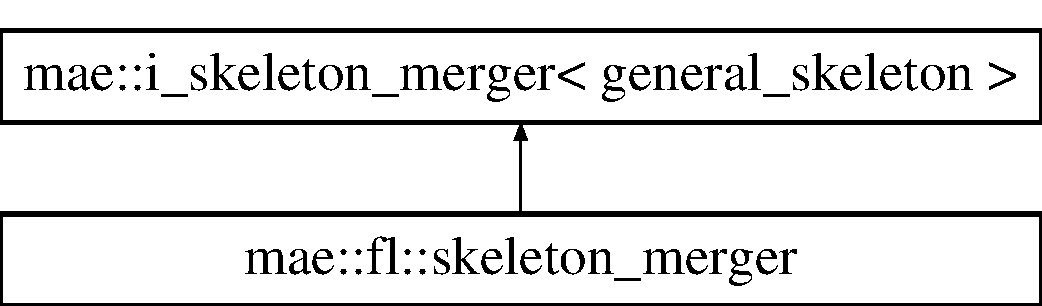
\includegraphics[height=2.000000cm]{classmae_1_1fl_1_1skeleton__merger}
\end{center}
\end{figure}
\subsection*{Public Member Functions}
\begin{DoxyCompactItemize}
\item 
\hyperlink{classmae_1_1fl_1_1skeleton__merger_a9fd639642fc6c6a40c4e3ee32d67cd3b}{skeleton\-\_\-merger} ()
\item 
virtual std\-::shared\-\_\-ptr\\*
$<$ \hyperlink{classmae_1_1general__skeleton}{general\-\_\-skeleton} $>$ \hyperlink{classmae_1_1fl_1_1skeleton__merger_aecb802bd58e39aa7bd09f71ba784df90}{merge} (std\-::vector$<$ std\-::shared\-\_\-ptr$<$ \hyperlink{classmae_1_1general__skeleton}{general\-\_\-skeleton} $>$ $>$ skeletons)
\item 
virtual std\-::vector\\*
$<$ std\-::shared\-\_\-ptr\\*
$<$ \hyperlink{classmae_1_1general__skeleton}{general\-\_\-skeleton} $>$ $>$ \hyperlink{classmae_1_1fl_1_1skeleton__merger_aefedbb5f4d930ac9b237b1a2e7295992}{merge} (std\-::vector$<$ std\-::vector$<$ std\-::shared\-\_\-ptr$<$ \hyperlink{classmae_1_1general__skeleton}{general\-\_\-skeleton} $>$ $>$ $>$ skeletons)
\item 
virtual std\-::vector\\*
$<$ std\-::shared\-\_\-ptr\\*
$<$ \hyperlink{classmae_1_1general__skeleton}{general\-\_\-skeleton} $>$ $>$ \hyperlink{classmae_1_1fl_1_1skeleton__merger_a4db272fd699c29926d771047a1535bdf}{merge\-\_\-find\-\_\-mapping} (std\-::vector$<$ std\-::vector$<$ std\-::shared\-\_\-ptr$<$ \hyperlink{classmae_1_1general__skeleton}{general\-\_\-skeleton} $>$ $>$ $>$ skeletons)
\end{DoxyCompactItemize}


\subsection{Constructor \& Destructor Documentation}
\hypertarget{classmae_1_1fl_1_1skeleton__merger_a9fd639642fc6c6a40c4e3ee32d67cd3b}{\index{mae\-::fl\-::skeleton\-\_\-merger@{mae\-::fl\-::skeleton\-\_\-merger}!skeleton\-\_\-merger@{skeleton\-\_\-merger}}
\index{skeleton\-\_\-merger@{skeleton\-\_\-merger}!mae::fl::skeleton_merger@{mae\-::fl\-::skeleton\-\_\-merger}}
\subsubsection[{skeleton\-\_\-merger}]{\setlength{\rightskip}{0pt plus 5cm}mae\-::fl\-::skeleton\-\_\-merger\-::skeleton\-\_\-merger (
\begin{DoxyParamCaption}
{}
\end{DoxyParamCaption}
)}}\label{classmae_1_1fl_1_1skeleton__merger_a9fd639642fc6c6a40c4e3ee32d67cd3b}
Creates a new skeleton merger which merges skeleton data. 

\subsection{Member Function Documentation}
\hypertarget{classmae_1_1fl_1_1skeleton__merger_aecb802bd58e39aa7bd09f71ba784df90}{\index{mae\-::fl\-::skeleton\-\_\-merger@{mae\-::fl\-::skeleton\-\_\-merger}!merge@{merge}}
\index{merge@{merge}!mae::fl::skeleton_merger@{mae\-::fl\-::skeleton\-\_\-merger}}
\subsubsection[{merge}]{\setlength{\rightskip}{0pt plus 5cm}std\-::shared\-\_\-ptr$<$ {\bf general\-\_\-skeleton} $>$ mae\-::fl\-::skeleton\-\_\-merger\-::merge (
\begin{DoxyParamCaption}
\item[{std\-::vector$<$ std\-::shared\-\_\-ptr$<$ {\bf general\-\_\-skeleton} $>$ $>$}]{skeletons}
\end{DoxyParamCaption}
)\hspace{0.3cm}{\ttfamily [virtual]}}}\label{classmae_1_1fl_1_1skeleton__merger_aecb802bd58e39aa7bd09f71ba784df90}
Merges several skeletons to one more accurate skeleton.


\begin{DoxyParams}{Parameters}
{\em skeletons} & The skeletons to be merged. \\
\hline
\end{DoxyParams}
\begin{DoxyReturn}{Returns}
The resulting skeleton. 
\end{DoxyReturn}


Implements \hyperlink{classmae_1_1i__skeleton__merger_a7681bbf15f70612f2b4d42ef7f6dce06}{mae\-::i\-\_\-skeleton\-\_\-merger$<$ general\-\_\-skeleton $>$}.

\hypertarget{classmae_1_1fl_1_1skeleton__merger_aefedbb5f4d930ac9b237b1a2e7295992}{\index{mae\-::fl\-::skeleton\-\_\-merger@{mae\-::fl\-::skeleton\-\_\-merger}!merge@{merge}}
\index{merge@{merge}!mae::fl::skeleton_merger@{mae\-::fl\-::skeleton\-\_\-merger}}
\subsubsection[{merge}]{\setlength{\rightskip}{0pt plus 5cm}std\-::vector$<$ std\-::shared\-\_\-ptr$<$ {\bf general\-\_\-skeleton} $>$ $>$ mae\-::fl\-::skeleton\-\_\-merger\-::merge (
\begin{DoxyParamCaption}
\item[{std\-::vector$<$ std\-::vector$<$ std\-::shared\-\_\-ptr$<$ {\bf general\-\_\-skeleton} $>$ $>$ $>$}]{skeletons}
\end{DoxyParamCaption}
)\hspace{0.3cm}{\ttfamily [virtual]}}}\label{classmae_1_1fl_1_1skeleton__merger_aefedbb5f4d930ac9b237b1a2e7295992}
Merges all skeletons in one bin into a new skeleton. This means that the outer vector is processed by index and all skeletons in this container are merged.


\begin{DoxyParams}{Parameters}
{\em skeletons} & The skeletons to be merged. \\
\hline
\end{DoxyParams}
\begin{DoxyReturn}{Returns}
The merged skeletons. 
\end{DoxyReturn}


Implements \hyperlink{classmae_1_1i__skeleton__merger_a8639fcf9a372382401362ab63a5d049c}{mae\-::i\-\_\-skeleton\-\_\-merger$<$ general\-\_\-skeleton $>$}.

\hypertarget{classmae_1_1fl_1_1skeleton__merger_a4db272fd699c29926d771047a1535bdf}{\index{mae\-::fl\-::skeleton\-\_\-merger@{mae\-::fl\-::skeleton\-\_\-merger}!merge\-\_\-find\-\_\-mapping@{merge\-\_\-find\-\_\-mapping}}
\index{merge\-\_\-find\-\_\-mapping@{merge\-\_\-find\-\_\-mapping}!mae::fl::skeleton_merger@{mae\-::fl\-::skeleton\-\_\-merger}}
\subsubsection[{merge\-\_\-find\-\_\-mapping}]{\setlength{\rightskip}{0pt plus 5cm}std\-::vector$<$ std\-::shared\-\_\-ptr$<$ {\bf general\-\_\-skeleton} $>$ $>$ mae\-::fl\-::skeleton\-\_\-merger\-::merge\-\_\-find\-\_\-mapping (
\begin{DoxyParamCaption}
\item[{std\-::vector$<$ std\-::vector$<$ std\-::shared\-\_\-ptr$<$ {\bf general\-\_\-skeleton} $>$ $>$ $>$}]{skeletons}
\end{DoxyParamCaption}
)\hspace{0.3cm}{\ttfamily [virtual]}}}\label{classmae_1_1fl_1_1skeleton__merger_a4db272fd699c29926d771047a1535bdf}
Merges the skeleton data, which is present in data per stream, by finding a mapping for the skeletons and then merging the mapped skeletons. This means that the outer vector has one element for each stream and the inner vector represents the skeleton data of the different users on that stream.


\begin{DoxyParams}{Parameters}
{\em skeletons} & The skeleton data. \\
\hline
\end{DoxyParams}
\begin{DoxyReturn}{Returns}
The merged skeletons. 
\end{DoxyReturn}


Implements \hyperlink{classmae_1_1i__skeleton__merger_a7b783640e2d89d52cf40be5c5e2c9a6b}{mae\-::i\-\_\-skeleton\-\_\-merger$<$ general\-\_\-skeleton $>$}.



The documentation for this class was generated from the following files\-:\begin{DoxyCompactItemize}
\item 
src/mae/fl/skeleton\-\_\-merger.\-hpp\item 
src/mae/fl/skeleton\-\_\-merger.\-cpp\end{DoxyCompactItemize}

\hypertarget{classmae_1_1fl_1_1laban_1_1mv_1_1space__measurement}{\section{mae\-:\-:fl\-:\-:laban\-:\-:mv\-:\-:space\-\_\-measurement Class Reference}
\label{classmae_1_1fl_1_1laban_1_1mv_1_1space__measurement}\index{mae\-::fl\-::laban\-::mv\-::space\-\_\-measurement@{mae\-::fl\-::laban\-::mv\-::space\-\_\-measurement}}
}
Inheritance diagram for mae\-:\-:fl\-:\-:laban\-:\-:mv\-:\-:space\-\_\-measurement\-:\begin{figure}[H]
\begin{center}
\leavevmode
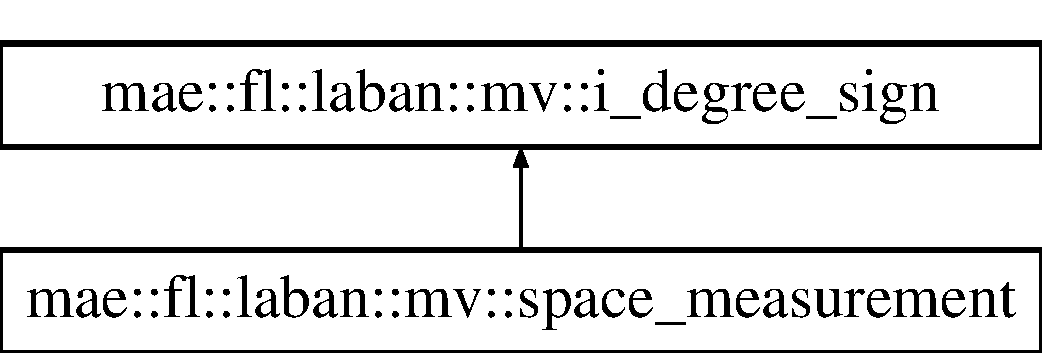
\includegraphics[height=2.000000cm]{classmae_1_1fl_1_1laban_1_1mv_1_1space__measurement}
\end{center}
\end{figure}
\subsection*{Public Member Functions}
\begin{DoxyCompactItemize}
\item 
\hyperlink{classmae_1_1fl_1_1laban_1_1mv_1_1space__measurement_ab8570e2e08f53abf9f8839fd0707ee33}{space\-\_\-measurement} (e\-\_\-space type, unsigned int degree, e\-\_\-space\-\_\-direction direction=e\-\_\-space\-\_\-direction\-::\-N\-O\-N\-E\-\_\-\-S\-P\-A\-C\-E\-\_\-\-D\-I\-R\-E\-C\-T\-I\-O\-N)
\item 
e\-\_\-space \hyperlink{classmae_1_1fl_1_1laban_1_1mv_1_1space__measurement_a6e49ae9e3c7a2c5b501b07835588f9cb}{get\-\_\-type} () const 
\item 
unsigned int \hyperlink{classmae_1_1fl_1_1laban_1_1mv_1_1space__measurement_a8ea28ebbc7ed2dbf875cb6be9e23798c}{get\-\_\-degree} () const 
\item 
e\-\_\-space\-\_\-direction \hyperlink{classmae_1_1fl_1_1laban_1_1mv_1_1space__measurement_a397a6a25188f5402a514c259b23ced78}{get\-\_\-direction} () const 
\item 
virtual bool \hyperlink{classmae_1_1fl_1_1laban_1_1mv_1_1space__measurement_a3dd6b152d30ec2d8cf62933f09e445cd}{equals} (std\-::shared\-\_\-ptr$<$ \hyperlink{classmae_1_1fl_1_1laban_1_1mv_1_1i__degree__sign}{i\-\_\-degree\-\_\-sign} $>$ a) const 
\item 
virtual std\-::string \hyperlink{classmae_1_1fl_1_1laban_1_1mv_1_1space__measurement_ab4121b6344f7dcbb4b7d11a3545de50a}{xml} (unsigned int indent=0, std\-::string namesp=\char`\"{}\char`\"{}, bool print\-\_\-type=false) const 
\item 
virtual std\-::string \hyperlink{classmae_1_1fl_1_1laban_1_1mv_1_1space__measurement_af68cab95083ca91bc99a9a45edc7ea86}{svg} (std\-::string identifier, double posx, double posy, double width, double height, bool left=false) const 
\item 
virtual std\-::string \hyperlink{classmae_1_1fl_1_1laban_1_1mv_1_1space__measurement_a58c0ec3d959b60b381441cf65cc1684a}{str} () const 
\end{DoxyCompactItemize}
\subsection*{Friends}
\begin{DoxyCompactItemize}
\item 
\hypertarget{classmae_1_1fl_1_1laban_1_1mv_1_1space__measurement_ab8647bc1a80ec53d5186da8088521fff}{std\-::ostream \& {\bfseries operator$<$$<$} (std\-::ostream \&os, const \hyperlink{classmae_1_1fl_1_1laban_1_1mv_1_1space__measurement}{space\-\_\-measurement} \&obj)}\label{classmae_1_1fl_1_1laban_1_1mv_1_1space__measurement_ab8647bc1a80ec53d5186da8088521fff}

\item 
\hypertarget{classmae_1_1fl_1_1laban_1_1mv_1_1space__measurement_af0effaf36edda89207afbef9cf7d4ded}{std\-::ostream \& {\bfseries operator$<$$<$} (std\-::ostream \&os, const std\-::shared\-\_\-ptr$<$ \hyperlink{classmae_1_1fl_1_1laban_1_1mv_1_1space__measurement}{space\-\_\-measurement} $>$ \&obj)}\label{classmae_1_1fl_1_1laban_1_1mv_1_1space__measurement_af0effaf36edda89207afbef9cf7d4ded}

\end{DoxyCompactItemize}


\subsection{Constructor \& Destructor Documentation}
\hypertarget{classmae_1_1fl_1_1laban_1_1mv_1_1space__measurement_ab8570e2e08f53abf9f8839fd0707ee33}{\index{mae\-::fl\-::laban\-::mv\-::space\-\_\-measurement@{mae\-::fl\-::laban\-::mv\-::space\-\_\-measurement}!space\-\_\-measurement@{space\-\_\-measurement}}
\index{space\-\_\-measurement@{space\-\_\-measurement}!mae::fl::laban::mv::space_measurement@{mae\-::fl\-::laban\-::mv\-::space\-\_\-measurement}}
\subsubsection[{space\-\_\-measurement}]{\setlength{\rightskip}{0pt plus 5cm}mae\-::fl\-::laban\-::mv\-::space\-\_\-measurement\-::space\-\_\-measurement (
\begin{DoxyParamCaption}
\item[{e\-\_\-space}]{type, }
\item[{unsigned int}]{degree, }
\item[{e\-\_\-space\-\_\-direction}]{direction = {\ttfamily e\-\_\-space\-\_\-direction\-:\-:NONE\-\_\-SPACE\-\_\-DIRECTION}}
\end{DoxyParamCaption}
)}}\label{classmae_1_1fl_1_1laban_1_1mv_1_1space__measurement_ab8570e2e08f53abf9f8839fd0707ee33}
Creates a space measurement sign. It is not to be confused with the space symbol which is a symbol that represents a space measurement and therefore contains one.


\begin{DoxyParams}{Parameters}
{\em type} & The type of the space measurement. \\
\hline
{\em degree} & The degree which is an integer between 1 and 6. \\
\hline
{\em direction} & (optional) The space direction (similiar to the (horizontal) direction of a direction symbol). \\
\hline
\end{DoxyParams}


\subsection{Member Function Documentation}
\hypertarget{classmae_1_1fl_1_1laban_1_1mv_1_1space__measurement_a3dd6b152d30ec2d8cf62933f09e445cd}{\index{mae\-::fl\-::laban\-::mv\-::space\-\_\-measurement@{mae\-::fl\-::laban\-::mv\-::space\-\_\-measurement}!equals@{equals}}
\index{equals@{equals}!mae::fl::laban::mv::space_measurement@{mae\-::fl\-::laban\-::mv\-::space\-\_\-measurement}}
\subsubsection[{equals}]{\setlength{\rightskip}{0pt plus 5cm}bool mae\-::fl\-::laban\-::mv\-::space\-\_\-measurement\-::equals (
\begin{DoxyParamCaption}
\item[{std\-::shared\-\_\-ptr$<$ {\bf i\-\_\-degree\-\_\-sign} $>$}]{a}
\end{DoxyParamCaption}
) const\hspace{0.3cm}{\ttfamily [virtual]}}}\label{classmae_1_1fl_1_1laban_1_1mv_1_1space__measurement_a3dd6b152d30ec2d8cf62933f09e445cd}
Compares this element to the given one and returns true if the elements are equal.


\begin{DoxyParams}{Parameters}
{\em a} & The element to be compared to. \\
\hline
\end{DoxyParams}
\begin{DoxyReturn}{Returns}
True if equal. 
\end{DoxyReturn}


Implements \hyperlink{classmae_1_1fl_1_1laban_1_1mv_1_1i__degree__sign_a65fee11b31d29709fd4022f90f4638bd}{mae\-::fl\-::laban\-::mv\-::i\-\_\-degree\-\_\-sign}.

\hypertarget{classmae_1_1fl_1_1laban_1_1mv_1_1space__measurement_a8ea28ebbc7ed2dbf875cb6be9e23798c}{\index{mae\-::fl\-::laban\-::mv\-::space\-\_\-measurement@{mae\-::fl\-::laban\-::mv\-::space\-\_\-measurement}!get\-\_\-degree@{get\-\_\-degree}}
\index{get\-\_\-degree@{get\-\_\-degree}!mae::fl::laban::mv::space_measurement@{mae\-::fl\-::laban\-::mv\-::space\-\_\-measurement}}
\subsubsection[{get\-\_\-degree}]{\setlength{\rightskip}{0pt plus 5cm}unsigned int mae\-::fl\-::laban\-::mv\-::space\-\_\-measurement\-::get\-\_\-degree (
\begin{DoxyParamCaption}
{}
\end{DoxyParamCaption}
) const}}\label{classmae_1_1fl_1_1laban_1_1mv_1_1space__measurement_a8ea28ebbc7ed2dbf875cb6be9e23798c}
Returns the degree of the space measurement which is an integer between 1 and 6.

\begin{DoxyReturn}{Returns}
The degree. 
\end{DoxyReturn}
\hypertarget{classmae_1_1fl_1_1laban_1_1mv_1_1space__measurement_a397a6a25188f5402a514c259b23ced78}{\index{mae\-::fl\-::laban\-::mv\-::space\-\_\-measurement@{mae\-::fl\-::laban\-::mv\-::space\-\_\-measurement}!get\-\_\-direction@{get\-\_\-direction}}
\index{get\-\_\-direction@{get\-\_\-direction}!mae::fl::laban::mv::space_measurement@{mae\-::fl\-::laban\-::mv\-::space\-\_\-measurement}}
\subsubsection[{get\-\_\-direction}]{\setlength{\rightskip}{0pt plus 5cm}e\-\_\-space\-\_\-direction mae\-::fl\-::laban\-::mv\-::space\-\_\-measurement\-::get\-\_\-direction (
\begin{DoxyParamCaption}
{}
\end{DoxyParamCaption}
) const}}\label{classmae_1_1fl_1_1laban_1_1mv_1_1space__measurement_a397a6a25188f5402a514c259b23ced78}
Returns the space direction which is a horizontal direction similar to the (horizontal) direction of the direction symbols. Returns N\-O\-N\-E if this element is not set.

\begin{DoxyReturn}{Returns}
The space direction. 
\end{DoxyReturn}
\hypertarget{classmae_1_1fl_1_1laban_1_1mv_1_1space__measurement_a6e49ae9e3c7a2c5b501b07835588f9cb}{\index{mae\-::fl\-::laban\-::mv\-::space\-\_\-measurement@{mae\-::fl\-::laban\-::mv\-::space\-\_\-measurement}!get\-\_\-type@{get\-\_\-type}}
\index{get\-\_\-type@{get\-\_\-type}!mae::fl::laban::mv::space_measurement@{mae\-::fl\-::laban\-::mv\-::space\-\_\-measurement}}
\subsubsection[{get\-\_\-type}]{\setlength{\rightskip}{0pt plus 5cm}e\-\_\-space mae\-::fl\-::laban\-::mv\-::space\-\_\-measurement\-::get\-\_\-type (
\begin{DoxyParamCaption}
{}
\end{DoxyParamCaption}
) const}}\label{classmae_1_1fl_1_1laban_1_1mv_1_1space__measurement_a6e49ae9e3c7a2c5b501b07835588f9cb}
Returns the type of the space measurement.

\begin{DoxyReturn}{Returns}
The type. 
\end{DoxyReturn}
\hypertarget{classmae_1_1fl_1_1laban_1_1mv_1_1space__measurement_a58c0ec3d959b60b381441cf65cc1684a}{\index{mae\-::fl\-::laban\-::mv\-::space\-\_\-measurement@{mae\-::fl\-::laban\-::mv\-::space\-\_\-measurement}!str@{str}}
\index{str@{str}!mae::fl::laban::mv::space_measurement@{mae\-::fl\-::laban\-::mv\-::space\-\_\-measurement}}
\subsubsection[{str}]{\setlength{\rightskip}{0pt plus 5cm}std\-::string mae\-::fl\-::laban\-::mv\-::space\-\_\-measurement\-::str (
\begin{DoxyParamCaption}
{}
\end{DoxyParamCaption}
) const\hspace{0.3cm}{\ttfamily [virtual]}}}\label{classmae_1_1fl_1_1laban_1_1mv_1_1space__measurement_a58c0ec3d959b60b381441cf65cc1684a}
Returns the string representation for this element.

\begin{DoxyReturn}{Returns}
The string. 
\end{DoxyReturn}
\hypertarget{classmae_1_1fl_1_1laban_1_1mv_1_1space__measurement_af68cab95083ca91bc99a9a45edc7ea86}{\index{mae\-::fl\-::laban\-::mv\-::space\-\_\-measurement@{mae\-::fl\-::laban\-::mv\-::space\-\_\-measurement}!svg@{svg}}
\index{svg@{svg}!mae::fl::laban::mv::space_measurement@{mae\-::fl\-::laban\-::mv\-::space\-\_\-measurement}}
\subsubsection[{svg}]{\setlength{\rightskip}{0pt plus 5cm}std\-::string mae\-::fl\-::laban\-::mv\-::space\-\_\-measurement\-::svg (
\begin{DoxyParamCaption}
\item[{std\-::string}]{identifier, }
\item[{double}]{posx, }
\item[{double}]{posy, }
\item[{double}]{width, }
\item[{double}]{height, }
\item[{bool}]{left = {\ttfamily false}}
\end{DoxyParamCaption}
) const\hspace{0.3cm}{\ttfamily [virtual]}}}\label{classmae_1_1fl_1_1laban_1_1mv_1_1space__measurement_af68cab95083ca91bc99a9a45edc7ea86}
Returns the S\-V\-G representation for this symbol.


\begin{DoxyParams}{Parameters}
{\em posx} & The x position. \\
\hline
{\em posy} & The y position. \\
\hline
{\em width} & The width. \\
\hline
{\em height} & The height. \\
\hline
\end{DoxyParams}
\begin{DoxyReturn}{Returns}
The S\-V\-G. 
\end{DoxyReturn}


Implements \hyperlink{classmae_1_1fl_1_1laban_1_1mv_1_1i__degree__sign_abb3ff23c8dcaaa80b6062bf5f8162c51}{mae\-::fl\-::laban\-::mv\-::i\-\_\-degree\-\_\-sign}.

\hypertarget{classmae_1_1fl_1_1laban_1_1mv_1_1space__measurement_ab4121b6344f7dcbb4b7d11a3545de50a}{\index{mae\-::fl\-::laban\-::mv\-::space\-\_\-measurement@{mae\-::fl\-::laban\-::mv\-::space\-\_\-measurement}!xml@{xml}}
\index{xml@{xml}!mae::fl::laban::mv::space_measurement@{mae\-::fl\-::laban\-::mv\-::space\-\_\-measurement}}
\subsubsection[{xml}]{\setlength{\rightskip}{0pt plus 5cm}std\-::string mae\-::fl\-::laban\-::mv\-::space\-\_\-measurement\-::xml (
\begin{DoxyParamCaption}
\item[{unsigned int}]{indent = {\ttfamily 0}, }
\item[{std\-::string}]{namesp = {\ttfamily \char`\"{}\char`\"{}}, }
\item[{bool}]{print\-\_\-type = {\ttfamily false}}
\end{DoxyParamCaption}
) const\hspace{0.3cm}{\ttfamily [virtual]}}}\label{classmae_1_1fl_1_1laban_1_1mv_1_1space__measurement_ab4121b6344f7dcbb4b7d11a3545de50a}
Returns the X\-M\-L representation for this element.


\begin{DoxyParams}{Parameters}
{\em indent} & The applied indent. \\
\hline
{\em namesp} & The prefixed X\-M\-L namespace.\\
\hline
\end{DoxyParams}
\begin{DoxyReturn}{Returns}
The X\-M\-L string. 
\end{DoxyReturn}


Implements \hyperlink{classmae_1_1fl_1_1laban_1_1mv_1_1i__degree__sign_abddf8459a5231b204ac2f023633aa4c4}{mae\-::fl\-::laban\-::mv\-::i\-\_\-degree\-\_\-sign}.



The documentation for this class was generated from the following files\-:\begin{DoxyCompactItemize}
\item 
src/mae/fl/laban/mv/space\-\_\-measurement.\-hpp\item 
src/mae/fl/laban/mv/space\-\_\-measurement.\-cpp\end{DoxyCompactItemize}

\hypertarget{classmae_1_1fl_1_1laban_1_1mv_1_1space__symbol}{\section{mae\-:\-:fl\-:\-:laban\-:\-:mv\-:\-:space\-\_\-symbol Class Reference}
\label{classmae_1_1fl_1_1laban_1_1mv_1_1space__symbol}\index{mae\-::fl\-::laban\-::mv\-::space\-\_\-symbol@{mae\-::fl\-::laban\-::mv\-::space\-\_\-symbol}}
}
Inheritance diagram for mae\-:\-:fl\-:\-:laban\-:\-:mv\-:\-:space\-\_\-symbol\-:\begin{figure}[H]
\begin{center}
\leavevmode
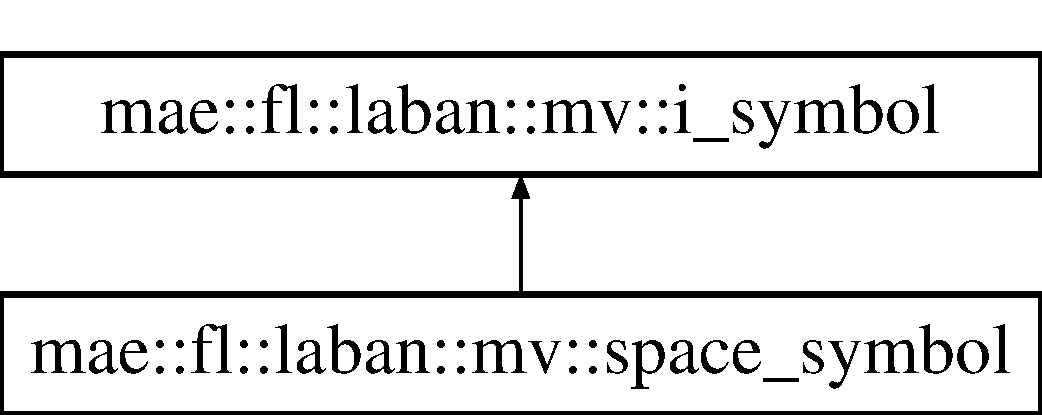
\includegraphics[height=2.000000cm]{classmae_1_1fl_1_1laban_1_1mv_1_1space__symbol}
\end{center}
\end{figure}
\subsection*{Public Member Functions}
\begin{DoxyCompactItemize}
\item 
\hyperlink{classmae_1_1fl_1_1laban_1_1mv_1_1space__symbol_ad39b3f3dbd05a06071f246680b175882}{space\-\_\-symbol} (std\-::shared\-\_\-ptr$<$ \hyperlink{classmae_1_1fl_1_1laban_1_1mv_1_1space__measurement}{space\-\_\-measurement} $>$ \hyperlink{classmae_1_1fl_1_1laban_1_1mv_1_1space__measurement}{space\-\_\-measurement}, std\-::shared\-\_\-ptr$<$ \hyperlink{classmae_1_1fl_1_1laban_1_1mv_1_1i__dynamics__sign}{i\-\_\-dynamics\-\_\-sign} $>$ dynamics=nullptr)
\item 
std\-::shared\-\_\-ptr$<$ \hyperlink{classmae_1_1fl_1_1laban_1_1mv_1_1i__dynamics__sign}{i\-\_\-dynamics\-\_\-sign} $>$ \hyperlink{classmae_1_1fl_1_1laban_1_1mv_1_1space__symbol_a5105e434045f777e6a0650c063ed815d}{get\-\_\-dynamics} () const 
\item 
std\-::shared\-\_\-ptr\\*
$<$ \hyperlink{classmae_1_1fl_1_1laban_1_1mv_1_1space__measurement}{space\-\_\-measurement} $>$ \hyperlink{classmae_1_1fl_1_1laban_1_1mv_1_1space__symbol_a090197af87afa823482359b9be18cb36}{get\-\_\-space\-\_\-measurement} () const 
\item 
virtual bool \hyperlink{classmae_1_1fl_1_1laban_1_1mv_1_1space__symbol_a9079a63e55fca3b2e8232fed1ef65e06}{equals} (std\-::shared\-\_\-ptr$<$ \hyperlink{classmae_1_1fl_1_1laban_1_1mv_1_1i__symbol}{i\-\_\-symbol} $>$ a) const 
\item 
virtual std\-::string \hyperlink{classmae_1_1fl_1_1laban_1_1mv_1_1space__symbol_a5aa4290ae8e7473dc5d0ef435f3035b7}{xml} (unsigned int indent=0, std\-::string namesp=\char`\"{}\char`\"{}) const 
\item 
virtual std\-::string \hyperlink{classmae_1_1fl_1_1laban_1_1mv_1_1space__symbol_ae6c9b408da1fcbc53881471035b496bd}{svg} (std\-::string identifier, double posx, double posy, double width, double height, bool left=false) const 
\item 
virtual std\-::string \hyperlink{classmae_1_1fl_1_1laban_1_1mv_1_1space__symbol_ac528043832637bf9186a3dda3604c418}{str} () const 
\end{DoxyCompactItemize}
\subsection*{Friends}
\begin{DoxyCompactItemize}
\item 
\hypertarget{classmae_1_1fl_1_1laban_1_1mv_1_1space__symbol_a60ed96abca4ada1a399e0248e4ec86a9}{std\-::ostream \& {\bfseries operator$<$$<$} (std\-::ostream \&os, const \hyperlink{classmae_1_1fl_1_1laban_1_1mv_1_1space__symbol}{space\-\_\-symbol} \&obj)}\label{classmae_1_1fl_1_1laban_1_1mv_1_1space__symbol_a60ed96abca4ada1a399e0248e4ec86a9}

\item 
\hypertarget{classmae_1_1fl_1_1laban_1_1mv_1_1space__symbol_a9b8face743ae5395fff7b3e4152213cc}{std\-::ostream \& {\bfseries operator$<$$<$} (std\-::ostream \&os, const std\-::shared\-\_\-ptr$<$ \hyperlink{classmae_1_1fl_1_1laban_1_1mv_1_1space__symbol}{space\-\_\-symbol} $>$ \&obj)}\label{classmae_1_1fl_1_1laban_1_1mv_1_1space__symbol_a9b8face743ae5395fff7b3e4152213cc}

\end{DoxyCompactItemize}


\subsection{Constructor \& Destructor Documentation}
\hypertarget{classmae_1_1fl_1_1laban_1_1mv_1_1space__symbol_ad39b3f3dbd05a06071f246680b175882}{\index{mae\-::fl\-::laban\-::mv\-::space\-\_\-symbol@{mae\-::fl\-::laban\-::mv\-::space\-\_\-symbol}!space\-\_\-symbol@{space\-\_\-symbol}}
\index{space\-\_\-symbol@{space\-\_\-symbol}!mae::fl::laban::mv::space_symbol@{mae\-::fl\-::laban\-::mv\-::space\-\_\-symbol}}
\subsubsection[{space\-\_\-symbol}]{\setlength{\rightskip}{0pt plus 5cm}mae\-::fl\-::laban\-::mv\-::space\-\_\-symbol\-::space\-\_\-symbol (
\begin{DoxyParamCaption}
\item[{std\-::shared\-\_\-ptr$<$ {\bf space\-\_\-measurement} $>$}]{space\-\_\-measurement, }
\item[{std\-::shared\-\_\-ptr$<$ {\bf i\-\_\-dynamics\-\_\-sign} $>$}]{dynamics = {\ttfamily nullptr}}
\end{DoxyParamCaption}
)}}\label{classmae_1_1fl_1_1laban_1_1mv_1_1space__symbol_ad39b3f3dbd05a06071f246680b175882}
Creates a new space symbol. It is not to be confused with the space measurement sign which is a member of this symbol.


\begin{DoxyParams}{Parameters}
{\em \hyperlink{classmae_1_1fl_1_1laban_1_1mv_1_1space__measurement}{space\-\_\-measurement}} & The space measurement sign. \\
\hline
{\em dynamics} & (optional) The dynamics sign. \\
\hline
\end{DoxyParams}


\subsection{Member Function Documentation}
\hypertarget{classmae_1_1fl_1_1laban_1_1mv_1_1space__symbol_a9079a63e55fca3b2e8232fed1ef65e06}{\index{mae\-::fl\-::laban\-::mv\-::space\-\_\-symbol@{mae\-::fl\-::laban\-::mv\-::space\-\_\-symbol}!equals@{equals}}
\index{equals@{equals}!mae::fl::laban::mv::space_symbol@{mae\-::fl\-::laban\-::mv\-::space\-\_\-symbol}}
\subsubsection[{equals}]{\setlength{\rightskip}{0pt plus 5cm}bool mae\-::fl\-::laban\-::mv\-::space\-\_\-symbol\-::equals (
\begin{DoxyParamCaption}
\item[{std\-::shared\-\_\-ptr$<$ {\bf i\-\_\-symbol} $>$}]{a}
\end{DoxyParamCaption}
) const\hspace{0.3cm}{\ttfamily [virtual]}}}\label{classmae_1_1fl_1_1laban_1_1mv_1_1space__symbol_a9079a63e55fca3b2e8232fed1ef65e06}
Returns true if signs are equal.


\begin{DoxyParams}{Parameters}
{\em a} & The sign to be compared to. \\
\hline
\end{DoxyParams}
\begin{DoxyReturn}{Returns}
True if equal. 
\end{DoxyReturn}


Implements \hyperlink{classmae_1_1fl_1_1laban_1_1mv_1_1i__symbol_a78d90af5e1da4a6561d7545a76689d0e}{mae\-::fl\-::laban\-::mv\-::i\-\_\-symbol}.

\hypertarget{classmae_1_1fl_1_1laban_1_1mv_1_1space__symbol_a5105e434045f777e6a0650c063ed815d}{\index{mae\-::fl\-::laban\-::mv\-::space\-\_\-symbol@{mae\-::fl\-::laban\-::mv\-::space\-\_\-symbol}!get\-\_\-dynamics@{get\-\_\-dynamics}}
\index{get\-\_\-dynamics@{get\-\_\-dynamics}!mae::fl::laban::mv::space_symbol@{mae\-::fl\-::laban\-::mv\-::space\-\_\-symbol}}
\subsubsection[{get\-\_\-dynamics}]{\setlength{\rightskip}{0pt plus 5cm}std\-::shared\-\_\-ptr$<$ {\bf i\-\_\-dynamics\-\_\-sign} $>$ mae\-::fl\-::laban\-::mv\-::space\-\_\-symbol\-::get\-\_\-dynamics (
\begin{DoxyParamCaption}
{}
\end{DoxyParamCaption}
) const}}\label{classmae_1_1fl_1_1laban_1_1mv_1_1space__symbol_a5105e434045f777e6a0650c063ed815d}
Returns the dynamics sign if any. Returns null otherwise.

\begin{DoxyReturn}{Returns}
A shared pointer to the dynamics sign. 
\end{DoxyReturn}
\hypertarget{classmae_1_1fl_1_1laban_1_1mv_1_1space__symbol_a090197af87afa823482359b9be18cb36}{\index{mae\-::fl\-::laban\-::mv\-::space\-\_\-symbol@{mae\-::fl\-::laban\-::mv\-::space\-\_\-symbol}!get\-\_\-space\-\_\-measurement@{get\-\_\-space\-\_\-measurement}}
\index{get\-\_\-space\-\_\-measurement@{get\-\_\-space\-\_\-measurement}!mae::fl::laban::mv::space_symbol@{mae\-::fl\-::laban\-::mv\-::space\-\_\-symbol}}
\subsubsection[{get\-\_\-space\-\_\-measurement}]{\setlength{\rightskip}{0pt plus 5cm}std\-::shared\-\_\-ptr$<$ {\bf space\-\_\-measurement} $>$ mae\-::fl\-::laban\-::mv\-::space\-\_\-symbol\-::get\-\_\-space\-\_\-measurement (
\begin{DoxyParamCaption}
{}
\end{DoxyParamCaption}
) const}}\label{classmae_1_1fl_1_1laban_1_1mv_1_1space__symbol_a090197af87afa823482359b9be18cb36}
Returns the space measurement sign.

\begin{DoxyReturn}{Returns}
The space measurement. 
\end{DoxyReturn}
\hypertarget{classmae_1_1fl_1_1laban_1_1mv_1_1space__symbol_ac528043832637bf9186a3dda3604c418}{\index{mae\-::fl\-::laban\-::mv\-::space\-\_\-symbol@{mae\-::fl\-::laban\-::mv\-::space\-\_\-symbol}!str@{str}}
\index{str@{str}!mae::fl::laban::mv::space_symbol@{mae\-::fl\-::laban\-::mv\-::space\-\_\-symbol}}
\subsubsection[{str}]{\setlength{\rightskip}{0pt plus 5cm}std\-::string mae\-::fl\-::laban\-::mv\-::space\-\_\-symbol\-::str (
\begin{DoxyParamCaption}
{}
\end{DoxyParamCaption}
) const\hspace{0.3cm}{\ttfamily [virtual]}}}\label{classmae_1_1fl_1_1laban_1_1mv_1_1space__symbol_ac528043832637bf9186a3dda3604c418}
Returns the string representation for this element.

\begin{DoxyReturn}{Returns}
The string. 
\end{DoxyReturn}


Implements \hyperlink{classmae_1_1fl_1_1laban_1_1mv_1_1i__symbol_ad254351eabf06ac945c168b24643872e}{mae\-::fl\-::laban\-::mv\-::i\-\_\-symbol}.

\hypertarget{classmae_1_1fl_1_1laban_1_1mv_1_1space__symbol_ae6c9b408da1fcbc53881471035b496bd}{\index{mae\-::fl\-::laban\-::mv\-::space\-\_\-symbol@{mae\-::fl\-::laban\-::mv\-::space\-\_\-symbol}!svg@{svg}}
\index{svg@{svg}!mae::fl::laban::mv::space_symbol@{mae\-::fl\-::laban\-::mv\-::space\-\_\-symbol}}
\subsubsection[{svg}]{\setlength{\rightskip}{0pt plus 5cm}std\-::string mae\-::fl\-::laban\-::mv\-::space\-\_\-symbol\-::svg (
\begin{DoxyParamCaption}
\item[{std\-::string}]{identifier, }
\item[{double}]{posx, }
\item[{double}]{posy, }
\item[{double}]{width, }
\item[{double}]{height, }
\item[{bool}]{left = {\ttfamily false}}
\end{DoxyParamCaption}
) const\hspace{0.3cm}{\ttfamily [virtual]}}}\label{classmae_1_1fl_1_1laban_1_1mv_1_1space__symbol_ae6c9b408da1fcbc53881471035b496bd}
Returns the S\-V\-G representation for this symbol.


\begin{DoxyParams}{Parameters}
{\em posx} & The x position. \\
\hline
{\em posy} & The y position. \\
\hline
{\em width} & The width. \\
\hline
{\em height} & The height. \\
\hline
\end{DoxyParams}
\begin{DoxyReturn}{Returns}
The S\-V\-G. 
\end{DoxyReturn}


Implements \hyperlink{classmae_1_1fl_1_1laban_1_1mv_1_1i__symbol_ae0a724c98c27c05fdde9afff99184029}{mae\-::fl\-::laban\-::mv\-::i\-\_\-symbol}.

\hypertarget{classmae_1_1fl_1_1laban_1_1mv_1_1space__symbol_a5aa4290ae8e7473dc5d0ef435f3035b7}{\index{mae\-::fl\-::laban\-::mv\-::space\-\_\-symbol@{mae\-::fl\-::laban\-::mv\-::space\-\_\-symbol}!xml@{xml}}
\index{xml@{xml}!mae::fl::laban::mv::space_symbol@{mae\-::fl\-::laban\-::mv\-::space\-\_\-symbol}}
\subsubsection[{xml}]{\setlength{\rightskip}{0pt plus 5cm}std\-::string mae\-::fl\-::laban\-::mv\-::space\-\_\-symbol\-::xml (
\begin{DoxyParamCaption}
\item[{unsigned int}]{indent = {\ttfamily 0}, }
\item[{std\-::string}]{namesp = {\ttfamily \char`\"{}\char`\"{}}}
\end{DoxyParamCaption}
) const\hspace{0.3cm}{\ttfamily [virtual]}}}\label{classmae_1_1fl_1_1laban_1_1mv_1_1space__symbol_a5aa4290ae8e7473dc5d0ef435f3035b7}
Returns the X\-M\-L representation for this element.


\begin{DoxyParams}{Parameters}
{\em indent} & The applied indent. \\
\hline
{\em namesp} & The prefixed X\-M\-L namespace.\\
\hline
\end{DoxyParams}
\begin{DoxyReturn}{Returns}
The X\-M\-L string. 
\end{DoxyReturn}


Implements \hyperlink{classmae_1_1fl_1_1laban_1_1mv_1_1i__symbol_a05d0b0c74bad854d5e9e3291bbd87b0d}{mae\-::fl\-::laban\-::mv\-::i\-\_\-symbol}.



The documentation for this class was generated from the following files\-:\begin{DoxyCompactItemize}
\item 
src/mae/fl/laban/mv/space\-\_\-symbol.\-hpp\item 
src/mae/fl/laban/mv/space\-\_\-symbol.\-cpp\end{DoxyCompactItemize}

\hypertarget{classmae_1_1fl_1_1laban_1_1ps_1_1surface__part}{\section{mae\-:\-:fl\-:\-:laban\-:\-:ps\-:\-:surface\-\_\-part Class Reference}
\label{classmae_1_1fl_1_1laban_1_1ps_1_1surface__part}\index{mae\-::fl\-::laban\-::ps\-::surface\-\_\-part@{mae\-::fl\-::laban\-::ps\-::surface\-\_\-part}}
}
Inheritance diagram for mae\-:\-:fl\-:\-:laban\-:\-:ps\-:\-:surface\-\_\-part\-:\begin{figure}[H]
\begin{center}
\leavevmode
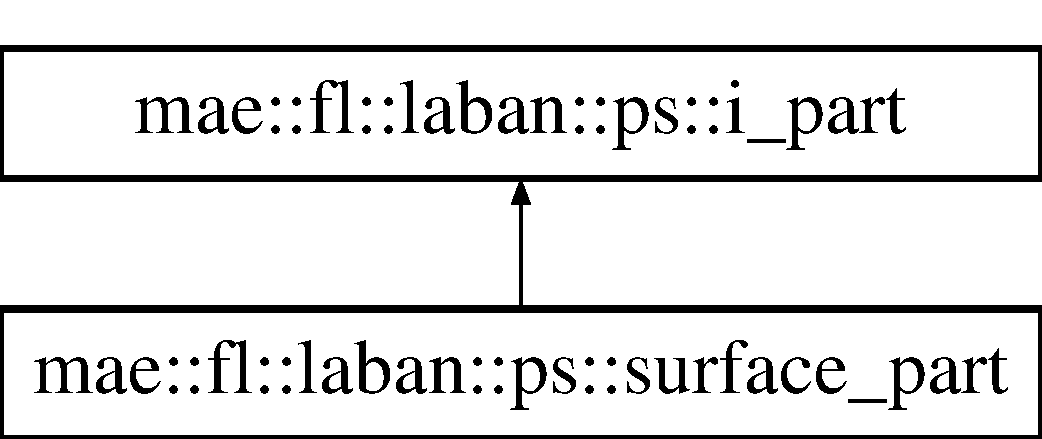
\includegraphics[height=2.000000cm]{classmae_1_1fl_1_1laban_1_1ps_1_1surface__part}
\end{center}
\end{figure}
\subsection*{Public Member Functions}
\begin{DoxyCompactItemize}
\item 
\hyperlink{classmae_1_1fl_1_1laban_1_1ps_1_1surface__part_a0a50c03195823029b001d0131cc78b9c}{surface\-\_\-part} (e\-\_\-limb\-\_\-side lside, std\-::shared\-\_\-ptr$<$ \hyperlink{classmae_1_1fl_1_1laban_1_1ps_1_1i__limb}{i\-\_\-limb} $>$ limb)
\item 
e\-\_\-limb\-\_\-side \hyperlink{classmae_1_1fl_1_1laban_1_1ps_1_1surface__part_a406c2c34f0a3fd4f52eb6d2aa6a1506f}{get\-\_\-limb\-\_\-side} () const 
\item 
std\-::shared\-\_\-ptr$<$ \hyperlink{classmae_1_1fl_1_1laban_1_1ps_1_1i__limb}{i\-\_\-limb} $>$ \hyperlink{classmae_1_1fl_1_1laban_1_1ps_1_1surface__part_afe1decc973947cf6ab5a142c2b3c8bc2}{get\-\_\-limb} () const 
\item 
virtual std\-::string \hyperlink{classmae_1_1fl_1_1laban_1_1ps_1_1surface__part_a1853ed550de38dbc7b1b38b6ff676904}{xml} (unsigned int indent=0, std\-::string namesp=\char`\"{}\char`\"{}) const 
\item 
virtual std\-::string \hyperlink{classmae_1_1fl_1_1laban_1_1ps_1_1surface__part_a91102bf6d87a18afa19ace304c4607e0}{svg} (std\-::string identifier, double posx, double posy, double width, double height, bool left=false) const 
\item 
virtual bool \hyperlink{classmae_1_1fl_1_1laban_1_1ps_1_1surface__part_a1ca1e44626d00dd7647927bafd86c266}{equals} (std\-::shared\-\_\-ptr$<$ \hyperlink{classmae_1_1fl_1_1laban_1_1ps_1_1i__part}{i\-\_\-part} $>$ a) const 
\end{DoxyCompactItemize}


\subsection{Constructor \& Destructor Documentation}
\hypertarget{classmae_1_1fl_1_1laban_1_1ps_1_1surface__part_a0a50c03195823029b001d0131cc78b9c}{\index{mae\-::fl\-::laban\-::ps\-::surface\-\_\-part@{mae\-::fl\-::laban\-::ps\-::surface\-\_\-part}!surface\-\_\-part@{surface\-\_\-part}}
\index{surface\-\_\-part@{surface\-\_\-part}!mae::fl::laban::ps::surface_part@{mae\-::fl\-::laban\-::ps\-::surface\-\_\-part}}
\subsubsection[{surface\-\_\-part}]{\setlength{\rightskip}{0pt plus 5cm}mae\-::fl\-::laban\-::ps\-::surface\-\_\-part\-::surface\-\_\-part (
\begin{DoxyParamCaption}
\item[{e\-\_\-limb\-\_\-side}]{lside, }
\item[{std\-::shared\-\_\-ptr$<$ {\bf i\-\_\-limb} $>$}]{limb}
\end{DoxyParamCaption}
)}}\label{classmae_1_1fl_1_1laban_1_1ps_1_1surface__part_a0a50c03195823029b001d0131cc78b9c}
Creates a surface body part sign.


\begin{DoxyParams}{Parameters}
{\em lside} & The addressed side of the limb. \\
\hline
{\em limb} & The addressed limb. \\
\hline
\end{DoxyParams}


\subsection{Member Function Documentation}
\hypertarget{classmae_1_1fl_1_1laban_1_1ps_1_1surface__part_a1ca1e44626d00dd7647927bafd86c266}{\index{mae\-::fl\-::laban\-::ps\-::surface\-\_\-part@{mae\-::fl\-::laban\-::ps\-::surface\-\_\-part}!equals@{equals}}
\index{equals@{equals}!mae::fl::laban::ps::surface_part@{mae\-::fl\-::laban\-::ps\-::surface\-\_\-part}}
\subsubsection[{equals}]{\setlength{\rightskip}{0pt plus 5cm}bool mae\-::fl\-::laban\-::ps\-::surface\-\_\-part\-::equals (
\begin{DoxyParamCaption}
\item[{std\-::shared\-\_\-ptr$<$ {\bf i\-\_\-part} $>$}]{a}
\end{DoxyParamCaption}
) const\hspace{0.3cm}{\ttfamily [virtual]}}}\label{classmae_1_1fl_1_1laban_1_1ps_1_1surface__part_a1ca1e44626d00dd7647927bafd86c266}
Returns true if elements are equal.


\begin{DoxyParams}{Parameters}
{\em a} & The element to be compared to. \\
\hline
\end{DoxyParams}
\begin{DoxyReturn}{Returns}
True if equal. 
\end{DoxyReturn}


Implements \hyperlink{classmae_1_1fl_1_1laban_1_1ps_1_1i__part_ad43f6b88cb409ac26342db51606ea1e1}{mae\-::fl\-::laban\-::ps\-::i\-\_\-part}.

\hypertarget{classmae_1_1fl_1_1laban_1_1ps_1_1surface__part_afe1decc973947cf6ab5a142c2b3c8bc2}{\index{mae\-::fl\-::laban\-::ps\-::surface\-\_\-part@{mae\-::fl\-::laban\-::ps\-::surface\-\_\-part}!get\-\_\-limb@{get\-\_\-limb}}
\index{get\-\_\-limb@{get\-\_\-limb}!mae::fl::laban::ps::surface_part@{mae\-::fl\-::laban\-::ps\-::surface\-\_\-part}}
\subsubsection[{get\-\_\-limb}]{\setlength{\rightskip}{0pt plus 5cm}std\-::shared\-\_\-ptr$<$ {\bf i\-\_\-limb} $>$ mae\-::fl\-::laban\-::ps\-::surface\-\_\-part\-::get\-\_\-limb (
\begin{DoxyParamCaption}
{}
\end{DoxyParamCaption}
) const}}\label{classmae_1_1fl_1_1laban_1_1ps_1_1surface__part_afe1decc973947cf6ab5a142c2b3c8bc2}
Returns the addressed limb.

\begin{DoxyReturn}{Returns}

\end{DoxyReturn}
\hypertarget{classmae_1_1fl_1_1laban_1_1ps_1_1surface__part_a406c2c34f0a3fd4f52eb6d2aa6a1506f}{\index{mae\-::fl\-::laban\-::ps\-::surface\-\_\-part@{mae\-::fl\-::laban\-::ps\-::surface\-\_\-part}!get\-\_\-limb\-\_\-side@{get\-\_\-limb\-\_\-side}}
\index{get\-\_\-limb\-\_\-side@{get\-\_\-limb\-\_\-side}!mae::fl::laban::ps::surface_part@{mae\-::fl\-::laban\-::ps\-::surface\-\_\-part}}
\subsubsection[{get\-\_\-limb\-\_\-side}]{\setlength{\rightskip}{0pt plus 5cm}e\-\_\-limb\-\_\-side mae\-::fl\-::laban\-::ps\-::surface\-\_\-part\-::get\-\_\-limb\-\_\-side (
\begin{DoxyParamCaption}
{}
\end{DoxyParamCaption}
) const}}\label{classmae_1_1fl_1_1laban_1_1ps_1_1surface__part_a406c2c34f0a3fd4f52eb6d2aa6a1506f}
Returns the addressed side of the limb.

\begin{DoxyReturn}{Returns}

\end{DoxyReturn}
\hypertarget{classmae_1_1fl_1_1laban_1_1ps_1_1surface__part_a91102bf6d87a18afa19ace304c4607e0}{\index{mae\-::fl\-::laban\-::ps\-::surface\-\_\-part@{mae\-::fl\-::laban\-::ps\-::surface\-\_\-part}!svg@{svg}}
\index{svg@{svg}!mae::fl::laban::ps::surface_part@{mae\-::fl\-::laban\-::ps\-::surface\-\_\-part}}
\subsubsection[{svg}]{\setlength{\rightskip}{0pt plus 5cm}std\-::string mae\-::fl\-::laban\-::ps\-::surface\-\_\-part\-::svg (
\begin{DoxyParamCaption}
\item[{std\-::string}]{identifier, }
\item[{double}]{posx, }
\item[{double}]{posy, }
\item[{double}]{width, }
\item[{double}]{height, }
\item[{bool}]{left = {\ttfamily false}}
\end{DoxyParamCaption}
) const\hspace{0.3cm}{\ttfamily [virtual]}}}\label{classmae_1_1fl_1_1laban_1_1ps_1_1surface__part_a91102bf6d87a18afa19ace304c4607e0}
Returns the S\-V\-G representation for this symbol.


\begin{DoxyParams}{Parameters}
{\em posx} & The x position. \\
\hline
{\em posy} & The y position. \\
\hline
{\em width} & The width. \\
\hline
{\em height} & The height. \\
\hline
\end{DoxyParams}
\begin{DoxyReturn}{Returns}
The S\-V\-G. 
\end{DoxyReturn}


Implements \hyperlink{classmae_1_1fl_1_1laban_1_1ps_1_1i__part_a78227d5ecd87655a7a9454c68f470368}{mae\-::fl\-::laban\-::ps\-::i\-\_\-part}.

\hypertarget{classmae_1_1fl_1_1laban_1_1ps_1_1surface__part_a1853ed550de38dbc7b1b38b6ff676904}{\index{mae\-::fl\-::laban\-::ps\-::surface\-\_\-part@{mae\-::fl\-::laban\-::ps\-::surface\-\_\-part}!xml@{xml}}
\index{xml@{xml}!mae::fl::laban::ps::surface_part@{mae\-::fl\-::laban\-::ps\-::surface\-\_\-part}}
\subsubsection[{xml}]{\setlength{\rightskip}{0pt plus 5cm}std\-::string mae\-::fl\-::laban\-::ps\-::surface\-\_\-part\-::xml (
\begin{DoxyParamCaption}
\item[{unsigned int}]{indent = {\ttfamily 0}, }
\item[{std\-::string}]{namesp = {\ttfamily \char`\"{}\char`\"{}}}
\end{DoxyParamCaption}
) const\hspace{0.3cm}{\ttfamily [virtual]}}}\label{classmae_1_1fl_1_1laban_1_1ps_1_1surface__part_a1853ed550de38dbc7b1b38b6ff676904}
Returns the X\-M\-L representation for this element.


\begin{DoxyParams}{Parameters}
{\em indent} & The applied indent. \\
\hline
{\em namesp} & The prefixed X\-M\-L namespace.\\
\hline
\end{DoxyParams}
\begin{DoxyReturn}{Returns}
The X\-M\-L string. 
\end{DoxyReturn}


Implements \hyperlink{classmae_1_1fl_1_1laban_1_1ps_1_1i__part_a704c07899099cdf53beb9187f23b7874}{mae\-::fl\-::laban\-::ps\-::i\-\_\-part}.



The documentation for this class was generated from the following files\-:\begin{DoxyCompactItemize}
\item 
src/mae/fl/laban/ps/surface\-\_\-part.\-hpp\item 
src/mae/fl/laban/ps/surface\-\_\-part.\-cpp\end{DoxyCompactItemize}

\hypertarget{classmae_1_1fl_1_1laban_1_1mv_1_1turn__symbol}{\section{mae\-:\-:fl\-:\-:laban\-:\-:mv\-:\-:turn\-\_\-symbol Class Reference}
\label{classmae_1_1fl_1_1laban_1_1mv_1_1turn__symbol}\index{mae\-::fl\-::laban\-::mv\-::turn\-\_\-symbol@{mae\-::fl\-::laban\-::mv\-::turn\-\_\-symbol}}
}
Inheritance diagram for mae\-:\-:fl\-:\-:laban\-:\-:mv\-:\-:turn\-\_\-symbol\-:\begin{figure}[H]
\begin{center}
\leavevmode
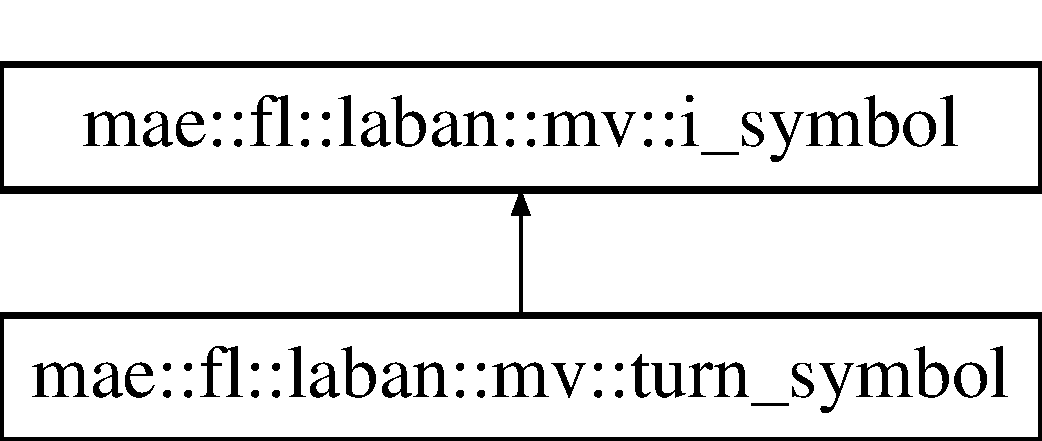
\includegraphics[height=2.000000cm]{classmae_1_1fl_1_1laban_1_1mv_1_1turn__symbol}
\end{center}
\end{figure}
\subsection*{Public Member Functions}
\begin{DoxyCompactItemize}
\item 
\hyperlink{classmae_1_1fl_1_1laban_1_1mv_1_1turn__symbol_a7b7f874e5277fb0122f9b219f03160e9}{turn\-\_\-symbol} (e\-\_\-turn\-\_\-direction direction, std\-::shared\-\_\-ptr$<$ \hyperlink{classmae_1_1fl_1_1laban_1_1mv_1_1i__dynamics__sign}{i\-\_\-dynamics\-\_\-sign} $>$ dynamics=nullptr, std\-::shared\-\_\-ptr$<$ \hyperlink{classmae_1_1fl_1_1laban_1_1mv_1_1i__degree__sign}{i\-\_\-degree\-\_\-sign} $>$ degree=nullptr)
\item 
e\-\_\-turn\-\_\-direction \hyperlink{classmae_1_1fl_1_1laban_1_1mv_1_1turn__symbol_a1e9aad7f2301dbd368858b57237fc8b7}{get\-\_\-direction} () const 
\item 
std\-::shared\-\_\-ptr$<$ \hyperlink{classmae_1_1fl_1_1laban_1_1mv_1_1i__dynamics__sign}{i\-\_\-dynamics\-\_\-sign} $>$ \hyperlink{classmae_1_1fl_1_1laban_1_1mv_1_1turn__symbol_ae9a052b0499ae07cbec21f7a224e31a1}{get\-\_\-dynamics} () const 
\item 
std\-::shared\-\_\-ptr$<$ \hyperlink{classmae_1_1fl_1_1laban_1_1mv_1_1i__degree__sign}{i\-\_\-degree\-\_\-sign} $>$ \hyperlink{classmae_1_1fl_1_1laban_1_1mv_1_1turn__symbol_af3aaa2ffaa36f2097e2f236e62b0bb47}{get\-\_\-degree} () const 
\item 
virtual bool \hyperlink{classmae_1_1fl_1_1laban_1_1mv_1_1turn__symbol_aafc1b11568db52d9fa3fbc86a7c281c2}{equals} (std\-::shared\-\_\-ptr$<$ \hyperlink{classmae_1_1fl_1_1laban_1_1mv_1_1i__symbol}{i\-\_\-symbol} $>$ a) const 
\item 
virtual std\-::string \hyperlink{classmae_1_1fl_1_1laban_1_1mv_1_1turn__symbol_a4b404fcb4b74a4db80b47cabb7876afa}{xml} (unsigned int indent=0, std\-::string namesp=\char`\"{}\char`\"{}) const 
\item 
virtual std\-::string \hyperlink{classmae_1_1fl_1_1laban_1_1mv_1_1turn__symbol_a756844c1207460af1d2f08245f0128b9}{svg} (std\-::string identifier, double posx, double posy, double width, double height, bool left=false) const 
\item 
virtual std\-::string \hyperlink{classmae_1_1fl_1_1laban_1_1mv_1_1turn__symbol_a92bc9681ef076940af9412fde943cf0c}{str} () const 
\end{DoxyCompactItemize}
\subsection*{Friends}
\begin{DoxyCompactItemize}
\item 
\hypertarget{classmae_1_1fl_1_1laban_1_1mv_1_1turn__symbol_a91823b0b8595839c893cf5e8b20ca7ec}{std\-::ostream \& {\bfseries operator$<$$<$} (std\-::ostream \&os, const \hyperlink{classmae_1_1fl_1_1laban_1_1mv_1_1turn__symbol}{turn\-\_\-symbol} \&obj)}\label{classmae_1_1fl_1_1laban_1_1mv_1_1turn__symbol_a91823b0b8595839c893cf5e8b20ca7ec}

\item 
\hypertarget{classmae_1_1fl_1_1laban_1_1mv_1_1turn__symbol_aa5cc7c2e13130c9d0e32d7a3b62dbcf4}{std\-::ostream \& {\bfseries operator$<$$<$} (std\-::ostream \&os, const std\-::shared\-\_\-ptr$<$ \hyperlink{classmae_1_1fl_1_1laban_1_1mv_1_1turn__symbol}{turn\-\_\-symbol} $>$ \&obj)}\label{classmae_1_1fl_1_1laban_1_1mv_1_1turn__symbol_aa5cc7c2e13130c9d0e32d7a3b62dbcf4}

\end{DoxyCompactItemize}


\subsection{Constructor \& Destructor Documentation}
\hypertarget{classmae_1_1fl_1_1laban_1_1mv_1_1turn__symbol_a7b7f874e5277fb0122f9b219f03160e9}{\index{mae\-::fl\-::laban\-::mv\-::turn\-\_\-symbol@{mae\-::fl\-::laban\-::mv\-::turn\-\_\-symbol}!turn\-\_\-symbol@{turn\-\_\-symbol}}
\index{turn\-\_\-symbol@{turn\-\_\-symbol}!mae::fl::laban::mv::turn_symbol@{mae\-::fl\-::laban\-::mv\-::turn\-\_\-symbol}}
\subsubsection[{turn\-\_\-symbol}]{\setlength{\rightskip}{0pt plus 5cm}mae\-::fl\-::laban\-::mv\-::turn\-\_\-symbol\-::turn\-\_\-symbol (
\begin{DoxyParamCaption}
\item[{e\-\_\-turn\-\_\-direction}]{direction, }
\item[{std\-::shared\-\_\-ptr$<$ {\bf i\-\_\-dynamics\-\_\-sign} $>$}]{dynamics = {\ttfamily nullptr}, }
\item[{std\-::shared\-\_\-ptr$<$ {\bf i\-\_\-degree\-\_\-sign} $>$}]{degree = {\ttfamily nullptr}}
\end{DoxyParamCaption}
)}}\label{classmae_1_1fl_1_1laban_1_1mv_1_1turn__symbol_a7b7f874e5277fb0122f9b219f03160e9}
Returns a turn symbol.


\begin{DoxyParams}{Parameters}
{\em direction} & The direction of the turn. \\
\hline
{\em dynamics} & (optional) An attached dynamics sign. Use null if unused and degree is required. \\
\hline
{\em degree} & (optional) The degree of the turn \\
\hline
\end{DoxyParams}


\subsection{Member Function Documentation}
\hypertarget{classmae_1_1fl_1_1laban_1_1mv_1_1turn__symbol_aafc1b11568db52d9fa3fbc86a7c281c2}{\index{mae\-::fl\-::laban\-::mv\-::turn\-\_\-symbol@{mae\-::fl\-::laban\-::mv\-::turn\-\_\-symbol}!equals@{equals}}
\index{equals@{equals}!mae::fl::laban::mv::turn_symbol@{mae\-::fl\-::laban\-::mv\-::turn\-\_\-symbol}}
\subsubsection[{equals}]{\setlength{\rightskip}{0pt plus 5cm}bool mae\-::fl\-::laban\-::mv\-::turn\-\_\-symbol\-::equals (
\begin{DoxyParamCaption}
\item[{std\-::shared\-\_\-ptr$<$ {\bf i\-\_\-symbol} $>$}]{a}
\end{DoxyParamCaption}
) const\hspace{0.3cm}{\ttfamily [virtual]}}}\label{classmae_1_1fl_1_1laban_1_1mv_1_1turn__symbol_aafc1b11568db52d9fa3fbc86a7c281c2}
Returns true if signs are equal.


\begin{DoxyParams}{Parameters}
{\em a} & The sign to be compared to. \\
\hline
\end{DoxyParams}
\begin{DoxyReturn}{Returns}
True if equal. 
\end{DoxyReturn}


Implements \hyperlink{classmae_1_1fl_1_1laban_1_1mv_1_1i__symbol_a78d90af5e1da4a6561d7545a76689d0e}{mae\-::fl\-::laban\-::mv\-::i\-\_\-symbol}.

\hypertarget{classmae_1_1fl_1_1laban_1_1mv_1_1turn__symbol_af3aaa2ffaa36f2097e2f236e62b0bb47}{\index{mae\-::fl\-::laban\-::mv\-::turn\-\_\-symbol@{mae\-::fl\-::laban\-::mv\-::turn\-\_\-symbol}!get\-\_\-degree@{get\-\_\-degree}}
\index{get\-\_\-degree@{get\-\_\-degree}!mae::fl::laban::mv::turn_symbol@{mae\-::fl\-::laban\-::mv\-::turn\-\_\-symbol}}
\subsubsection[{get\-\_\-degree}]{\setlength{\rightskip}{0pt plus 5cm}std\-::shared\-\_\-ptr$<$ {\bf i\-\_\-degree\-\_\-sign} $>$ mae\-::fl\-::laban\-::mv\-::turn\-\_\-symbol\-::get\-\_\-degree (
\begin{DoxyParamCaption}
{}
\end{DoxyParamCaption}
) const}}\label{classmae_1_1fl_1_1laban_1_1mv_1_1turn__symbol_af3aaa2ffaa36f2097e2f236e62b0bb47}
Returns the degree of the turn if set. Returns null otherwise.

\begin{DoxyReturn}{Returns}
The degree sign. 
\end{DoxyReturn}
\hypertarget{classmae_1_1fl_1_1laban_1_1mv_1_1turn__symbol_a1e9aad7f2301dbd368858b57237fc8b7}{\index{mae\-::fl\-::laban\-::mv\-::turn\-\_\-symbol@{mae\-::fl\-::laban\-::mv\-::turn\-\_\-symbol}!get\-\_\-direction@{get\-\_\-direction}}
\index{get\-\_\-direction@{get\-\_\-direction}!mae::fl::laban::mv::turn_symbol@{mae\-::fl\-::laban\-::mv\-::turn\-\_\-symbol}}
\subsubsection[{get\-\_\-direction}]{\setlength{\rightskip}{0pt plus 5cm}e\-\_\-turn\-\_\-direction mae\-::fl\-::laban\-::mv\-::turn\-\_\-symbol\-::get\-\_\-direction (
\begin{DoxyParamCaption}
{}
\end{DoxyParamCaption}
) const}}\label{classmae_1_1fl_1_1laban_1_1mv_1_1turn__symbol_a1e9aad7f2301dbd368858b57237fc8b7}
Return the direction of the turn.

\begin{DoxyReturn}{Returns}
The direction. 
\end{DoxyReturn}
\hypertarget{classmae_1_1fl_1_1laban_1_1mv_1_1turn__symbol_ae9a052b0499ae07cbec21f7a224e31a1}{\index{mae\-::fl\-::laban\-::mv\-::turn\-\_\-symbol@{mae\-::fl\-::laban\-::mv\-::turn\-\_\-symbol}!get\-\_\-dynamics@{get\-\_\-dynamics}}
\index{get\-\_\-dynamics@{get\-\_\-dynamics}!mae::fl::laban::mv::turn_symbol@{mae\-::fl\-::laban\-::mv\-::turn\-\_\-symbol}}
\subsubsection[{get\-\_\-dynamics}]{\setlength{\rightskip}{0pt plus 5cm}std\-::shared\-\_\-ptr$<$ {\bf i\-\_\-dynamics\-\_\-sign} $>$ mae\-::fl\-::laban\-::mv\-::turn\-\_\-symbol\-::get\-\_\-dynamics (
\begin{DoxyParamCaption}
{}
\end{DoxyParamCaption}
) const}}\label{classmae_1_1fl_1_1laban_1_1mv_1_1turn__symbol_ae9a052b0499ae07cbec21f7a224e31a1}
Returns the dynamics sign if any. Returns null otherwise.

\begin{DoxyReturn}{Returns}
The dynamics sign. 
\end{DoxyReturn}
\hypertarget{classmae_1_1fl_1_1laban_1_1mv_1_1turn__symbol_a92bc9681ef076940af9412fde943cf0c}{\index{mae\-::fl\-::laban\-::mv\-::turn\-\_\-symbol@{mae\-::fl\-::laban\-::mv\-::turn\-\_\-symbol}!str@{str}}
\index{str@{str}!mae::fl::laban::mv::turn_symbol@{mae\-::fl\-::laban\-::mv\-::turn\-\_\-symbol}}
\subsubsection[{str}]{\setlength{\rightskip}{0pt plus 5cm}std\-::string mae\-::fl\-::laban\-::mv\-::turn\-\_\-symbol\-::str (
\begin{DoxyParamCaption}
{}
\end{DoxyParamCaption}
) const\hspace{0.3cm}{\ttfamily [virtual]}}}\label{classmae_1_1fl_1_1laban_1_1mv_1_1turn__symbol_a92bc9681ef076940af9412fde943cf0c}
Returns the string representation for this element.

\begin{DoxyReturn}{Returns}
The string. 
\end{DoxyReturn}


Implements \hyperlink{classmae_1_1fl_1_1laban_1_1mv_1_1i__symbol_ad254351eabf06ac945c168b24643872e}{mae\-::fl\-::laban\-::mv\-::i\-\_\-symbol}.

\hypertarget{classmae_1_1fl_1_1laban_1_1mv_1_1turn__symbol_a756844c1207460af1d2f08245f0128b9}{\index{mae\-::fl\-::laban\-::mv\-::turn\-\_\-symbol@{mae\-::fl\-::laban\-::mv\-::turn\-\_\-symbol}!svg@{svg}}
\index{svg@{svg}!mae::fl::laban::mv::turn_symbol@{mae\-::fl\-::laban\-::mv\-::turn\-\_\-symbol}}
\subsubsection[{svg}]{\setlength{\rightskip}{0pt plus 5cm}std\-::string mae\-::fl\-::laban\-::mv\-::turn\-\_\-symbol\-::svg (
\begin{DoxyParamCaption}
\item[{std\-::string}]{identifier, }
\item[{double}]{posx, }
\item[{double}]{posy, }
\item[{double}]{width, }
\item[{double}]{height, }
\item[{bool}]{left = {\ttfamily false}}
\end{DoxyParamCaption}
) const\hspace{0.3cm}{\ttfamily [virtual]}}}\label{classmae_1_1fl_1_1laban_1_1mv_1_1turn__symbol_a756844c1207460af1d2f08245f0128b9}
Returns the S\-V\-G representation for this symbol.


\begin{DoxyParams}{Parameters}
{\em posx} & The x position. \\
\hline
{\em posy} & The y position. \\
\hline
{\em width} & The width. \\
\hline
{\em height} & The height. \\
\hline
\end{DoxyParams}
\begin{DoxyReturn}{Returns}
The S\-V\-G. 
\end{DoxyReturn}


Implements \hyperlink{classmae_1_1fl_1_1laban_1_1mv_1_1i__symbol_ae0a724c98c27c05fdde9afff99184029}{mae\-::fl\-::laban\-::mv\-::i\-\_\-symbol}.

\hypertarget{classmae_1_1fl_1_1laban_1_1mv_1_1turn__symbol_a4b404fcb4b74a4db80b47cabb7876afa}{\index{mae\-::fl\-::laban\-::mv\-::turn\-\_\-symbol@{mae\-::fl\-::laban\-::mv\-::turn\-\_\-symbol}!xml@{xml}}
\index{xml@{xml}!mae::fl::laban::mv::turn_symbol@{mae\-::fl\-::laban\-::mv\-::turn\-\_\-symbol}}
\subsubsection[{xml}]{\setlength{\rightskip}{0pt plus 5cm}std\-::string mae\-::fl\-::laban\-::mv\-::turn\-\_\-symbol\-::xml (
\begin{DoxyParamCaption}
\item[{unsigned int}]{indent = {\ttfamily 0}, }
\item[{std\-::string}]{namesp = {\ttfamily \char`\"{}\char`\"{}}}
\end{DoxyParamCaption}
) const\hspace{0.3cm}{\ttfamily [virtual]}}}\label{classmae_1_1fl_1_1laban_1_1mv_1_1turn__symbol_a4b404fcb4b74a4db80b47cabb7876afa}
Returns the X\-M\-L representation for this element.


\begin{DoxyParams}{Parameters}
{\em indent} & The applied indent. \\
\hline
{\em namesp} & The prefixed X\-M\-L namespace.\\
\hline
\end{DoxyParams}
\begin{DoxyReturn}{Returns}
The X\-M\-L string. 
\end{DoxyReturn}


Implements \hyperlink{classmae_1_1fl_1_1laban_1_1mv_1_1i__symbol_a05d0b0c74bad854d5e9e3291bbd87b0d}{mae\-::fl\-::laban\-::mv\-::i\-\_\-symbol}.



The documentation for this class was generated from the following files\-:\begin{DoxyCompactItemize}
\item 
src/mae/fl/laban/mv/turn\-\_\-symbol.\-hpp\item 
src/mae/fl/laban/mv/turn\-\_\-symbol.\-cpp\end{DoxyCompactItemize}

\hypertarget{classmae_1_1math_1_1vec3d}{\section{mae\-:\-:math\-:\-:vec3d Class Reference}
\label{classmae_1_1math_1_1vec3d}\index{mae\-::math\-::vec3d@{mae\-::math\-::vec3d}}
}
\subsection*{Public Member Functions}
\begin{DoxyCompactItemize}
\item 
\hyperlink{classmae_1_1math_1_1vec3d_a765884440bd75fb021f82a0b08342993}{vec3d} ()
\item 
\hyperlink{classmae_1_1math_1_1vec3d_a54c773be8273c8462df6ae790528ad90}{vec3d} (double x, double y, double z)
\item 
virtual void \hyperlink{classmae_1_1math_1_1vec3d_af152b95813c55f7136cd876df08da688}{set\-\_\-x} (double x)
\item 
virtual double \hyperlink{classmae_1_1math_1_1vec3d_a5ece2226e5d958b7d194b7011523cb45}{get\-\_\-x} () const 
\item 
virtual void \hyperlink{classmae_1_1math_1_1vec3d_acc4c161f86f5accfc477dc4eaa495477}{set\-\_\-y} (double y)
\item 
virtual double \hyperlink{classmae_1_1math_1_1vec3d_a42d97fc5d73175e3b48f3754491e2bbb}{get\-\_\-y} () const 
\item 
virtual void \hyperlink{classmae_1_1math_1_1vec3d_a2f447c43b1cce7f1e9d92a4a0632ff82}{set\-\_\-z} (double z)
\item 
virtual double \hyperlink{classmae_1_1math_1_1vec3d_a9597a58bdb1692d0a96bdb6e1368255e}{get\-\_\-z} () const 
\item 
virtual std\-::shared\-\_\-ptr$<$ \hyperlink{classmae_1_1math_1_1vec3d}{vec3d} $>$ \hyperlink{classmae_1_1math_1_1vec3d_a6cdd8d6e63078c444a048a4e68ae3819}{add} (std\-::shared\-\_\-ptr$<$ \hyperlink{classmae_1_1math_1_1vec3d}{vec3d} $>$ vec) const 
\item 
virtual std\-::shared\-\_\-ptr$<$ \hyperlink{classmae_1_1math_1_1vec3d}{vec3d} $>$ \hyperlink{classmae_1_1math_1_1vec3d_ab01f1ea5f0178f1d363df0d6f5465cab}{subtract} (std\-::shared\-\_\-ptr$<$ \hyperlink{classmae_1_1math_1_1vec3d}{vec3d} $>$ vec) const 
\item 
virtual std\-::shared\-\_\-ptr$<$ \hyperlink{classmae_1_1math_1_1vec3d}{vec3d} $>$ \hyperlink{classmae_1_1math_1_1vec3d_a3b96adb108c895bd488759ceecd40205}{normalize} () const 
\item 
virtual double \hyperlink{classmae_1_1math_1_1vec3d_aef0ce4fe306e9b6ae0dc26cb4ef123bf}{l2\-\_\-norm} () const 
\item 
virtual double \hyperlink{classmae_1_1math_1_1vec3d_a38ae714ef3e525af20c1a31b8c537406}{dot} (std\-::shared\-\_\-ptr$<$ \hyperlink{classmae_1_1math_1_1vec3d}{vec3d} $>$ vec) const 
\item 
virtual std\-::shared\-\_\-ptr$<$ \hyperlink{classmae_1_1math_1_1vec3d}{vec3d} $>$ \hyperlink{classmae_1_1math_1_1vec3d_aac2aed075aefc06722c7304f3d673eba}{cross} (std\-::shared\-\_\-ptr$<$ \hyperlink{classmae_1_1math_1_1vec3d}{vec3d} $>$ vec) const 
\item 
virtual std\-::string \hyperlink{classmae_1_1math_1_1vec3d_a686b7876881d3ffa6c51f9a538998c4a}{str} () const 
\end{DoxyCompactItemize}
\subsection*{Friends}
\begin{DoxyCompactItemize}
\item 
std\-::ostream \& \hyperlink{classmae_1_1math_1_1vec3d_a0639044d670a12dc86ce762c3370c731}{operator$<$$<$} (std\-::ostream \&os, const std\-::shared\-\_\-ptr$<$ \hyperlink{classmae_1_1math_1_1vec3d}{vec3d} $>$ \&obj)
\item 
std\-::ostream \& \hyperlink{classmae_1_1math_1_1vec3d_ab9143424a170891e76f764d1307d48e0}{operator$<$$<$} (std\-::ostream \&os, const \hyperlink{classmae_1_1math_1_1vec3d}{vec3d} \&obj)
\end{DoxyCompactItemize}


\subsection{Constructor \& Destructor Documentation}
\hypertarget{classmae_1_1math_1_1vec3d_a765884440bd75fb021f82a0b08342993}{\index{mae\-::math\-::vec3d@{mae\-::math\-::vec3d}!vec3d@{vec3d}}
\index{vec3d@{vec3d}!mae::math::vec3d@{mae\-::math\-::vec3d}}
\subsubsection[{vec3d}]{\setlength{\rightskip}{0pt plus 5cm}mae\-::math\-::vec3d\-::vec3d (
\begin{DoxyParamCaption}
{}
\end{DoxyParamCaption}
)}}\label{classmae_1_1math_1_1vec3d_a765884440bd75fb021f82a0b08342993}
Creates a new three dimensional vector with zeros as default values. \hypertarget{classmae_1_1math_1_1vec3d_a54c773be8273c8462df6ae790528ad90}{\index{mae\-::math\-::vec3d@{mae\-::math\-::vec3d}!vec3d@{vec3d}}
\index{vec3d@{vec3d}!mae::math::vec3d@{mae\-::math\-::vec3d}}
\subsubsection[{vec3d}]{\setlength{\rightskip}{0pt plus 5cm}mae\-::math\-::vec3d\-::vec3d (
\begin{DoxyParamCaption}
\item[{double}]{x, }
\item[{double}]{y, }
\item[{double}]{z}
\end{DoxyParamCaption}
)}}\label{classmae_1_1math_1_1vec3d_a54c773be8273c8462df6ae790528ad90}
Creates a new three dimensional vector.


\begin{DoxyParams}{Parameters}
{\em x} & The x value. \\
\hline
{\em y} & The y value. \\
\hline
{\em z} & The z value. \\
\hline
\end{DoxyParams}


\subsection{Member Function Documentation}
\hypertarget{classmae_1_1math_1_1vec3d_a6cdd8d6e63078c444a048a4e68ae3819}{\index{mae\-::math\-::vec3d@{mae\-::math\-::vec3d}!add@{add}}
\index{add@{add}!mae::math::vec3d@{mae\-::math\-::vec3d}}
\subsubsection[{add}]{\setlength{\rightskip}{0pt plus 5cm}std\-::shared\-\_\-ptr$<$ {\bf vec3d} $>$ mae\-::math\-::vec3d\-::add (
\begin{DoxyParamCaption}
\item[{std\-::shared\-\_\-ptr$<$ {\bf vec3d} $>$}]{vec}
\end{DoxyParamCaption}
) const\hspace{0.3cm}{\ttfamily [virtual]}}}\label{classmae_1_1math_1_1vec3d_a6cdd8d6e63078c444a048a4e68ae3819}
Adds the given vector's value to this vector's values and returns the result.

This vector is not changed.


\begin{DoxyParams}{Parameters}
{\em vec} & The vector to be added. \\
\hline
\end{DoxyParams}
\begin{DoxyReturn}{Returns}
The resulting vector. 
\end{DoxyReturn}
\hypertarget{classmae_1_1math_1_1vec3d_aac2aed075aefc06722c7304f3d673eba}{\index{mae\-::math\-::vec3d@{mae\-::math\-::vec3d}!cross@{cross}}
\index{cross@{cross}!mae::math::vec3d@{mae\-::math\-::vec3d}}
\subsubsection[{cross}]{\setlength{\rightskip}{0pt plus 5cm}std\-::shared\-\_\-ptr$<$ {\bf vec3d} $>$ mae\-::math\-::vec3d\-::cross (
\begin{DoxyParamCaption}
\item[{std\-::shared\-\_\-ptr$<$ {\bf vec3d} $>$}]{vec}
\end{DoxyParamCaption}
) const\hspace{0.3cm}{\ttfamily [virtual]}}}\label{classmae_1_1math_1_1vec3d_aac2aed075aefc06722c7304f3d673eba}
Returns the result of the cross product between the two vectors.


\begin{DoxyParams}{Parameters}
{\em vec} & The vector. \\
\hline
\end{DoxyParams}
\begin{DoxyReturn}{Returns}
The cross product. 
\end{DoxyReturn}
\hypertarget{classmae_1_1math_1_1vec3d_a38ae714ef3e525af20c1a31b8c537406}{\index{mae\-::math\-::vec3d@{mae\-::math\-::vec3d}!dot@{dot}}
\index{dot@{dot}!mae::math::vec3d@{mae\-::math\-::vec3d}}
\subsubsection[{dot}]{\setlength{\rightskip}{0pt plus 5cm}double mae\-::math\-::vec3d\-::dot (
\begin{DoxyParamCaption}
\item[{std\-::shared\-\_\-ptr$<$ {\bf vec3d} $>$}]{vec}
\end{DoxyParamCaption}
) const\hspace{0.3cm}{\ttfamily [virtual]}}}\label{classmae_1_1math_1_1vec3d_a38ae714ef3e525af20c1a31b8c537406}
Returns the result of the dot product between the two vectors.


\begin{DoxyParams}{Parameters}
{\em vec} & The vector. \\
\hline
\end{DoxyParams}
\begin{DoxyReturn}{Returns}
The dot product. 
\end{DoxyReturn}
\hypertarget{classmae_1_1math_1_1vec3d_a5ece2226e5d958b7d194b7011523cb45}{\index{mae\-::math\-::vec3d@{mae\-::math\-::vec3d}!get\-\_\-x@{get\-\_\-x}}
\index{get\-\_\-x@{get\-\_\-x}!mae::math::vec3d@{mae\-::math\-::vec3d}}
\subsubsection[{get\-\_\-x}]{\setlength{\rightskip}{0pt plus 5cm}double mae\-::math\-::vec3d\-::get\-\_\-x (
\begin{DoxyParamCaption}
{}
\end{DoxyParamCaption}
) const\hspace{0.3cm}{\ttfamily [virtual]}}}\label{classmae_1_1math_1_1vec3d_a5ece2226e5d958b7d194b7011523cb45}
Returns the x value of this vector.

\begin{DoxyReturn}{Returns}
x 
\end{DoxyReturn}
\hypertarget{classmae_1_1math_1_1vec3d_a42d97fc5d73175e3b48f3754491e2bbb}{\index{mae\-::math\-::vec3d@{mae\-::math\-::vec3d}!get\-\_\-y@{get\-\_\-y}}
\index{get\-\_\-y@{get\-\_\-y}!mae::math::vec3d@{mae\-::math\-::vec3d}}
\subsubsection[{get\-\_\-y}]{\setlength{\rightskip}{0pt plus 5cm}double mae\-::math\-::vec3d\-::get\-\_\-y (
\begin{DoxyParamCaption}
{}
\end{DoxyParamCaption}
) const\hspace{0.3cm}{\ttfamily [virtual]}}}\label{classmae_1_1math_1_1vec3d_a42d97fc5d73175e3b48f3754491e2bbb}
Returns the y value of this vector.

\begin{DoxyReturn}{Returns}
y 
\end{DoxyReturn}
\hypertarget{classmae_1_1math_1_1vec3d_a9597a58bdb1692d0a96bdb6e1368255e}{\index{mae\-::math\-::vec3d@{mae\-::math\-::vec3d}!get\-\_\-z@{get\-\_\-z}}
\index{get\-\_\-z@{get\-\_\-z}!mae::math::vec3d@{mae\-::math\-::vec3d}}
\subsubsection[{get\-\_\-z}]{\setlength{\rightskip}{0pt plus 5cm}double mae\-::math\-::vec3d\-::get\-\_\-z (
\begin{DoxyParamCaption}
{}
\end{DoxyParamCaption}
) const\hspace{0.3cm}{\ttfamily [virtual]}}}\label{classmae_1_1math_1_1vec3d_a9597a58bdb1692d0a96bdb6e1368255e}
Returns the z value of this vector.

\begin{DoxyReturn}{Returns}
z 
\end{DoxyReturn}
\hypertarget{classmae_1_1math_1_1vec3d_aef0ce4fe306e9b6ae0dc26cb4ef123bf}{\index{mae\-::math\-::vec3d@{mae\-::math\-::vec3d}!l2\-\_\-norm@{l2\-\_\-norm}}
\index{l2\-\_\-norm@{l2\-\_\-norm}!mae::math::vec3d@{mae\-::math\-::vec3d}}
\subsubsection[{l2\-\_\-norm}]{\setlength{\rightskip}{0pt plus 5cm}double mae\-::math\-::vec3d\-::l2\-\_\-norm (
\begin{DoxyParamCaption}
{}
\end{DoxyParamCaption}
) const\hspace{0.3cm}{\ttfamily [virtual]}}}\label{classmae_1_1math_1_1vec3d_aef0ce4fe306e9b6ae0dc26cb4ef123bf}
Returns the value of the L2 norm for this vector.

\begin{DoxyReturn}{Returns}
The norm value. 
\end{DoxyReturn}
\hypertarget{classmae_1_1math_1_1vec3d_a3b96adb108c895bd488759ceecd40205}{\index{mae\-::math\-::vec3d@{mae\-::math\-::vec3d}!normalize@{normalize}}
\index{normalize@{normalize}!mae::math::vec3d@{mae\-::math\-::vec3d}}
\subsubsection[{normalize}]{\setlength{\rightskip}{0pt plus 5cm}std\-::shared\-\_\-ptr$<$ {\bf vec3d} $>$ mae\-::math\-::vec3d\-::normalize (
\begin{DoxyParamCaption}
{}
\end{DoxyParamCaption}
) const\hspace{0.3cm}{\ttfamily [virtual]}}}\label{classmae_1_1math_1_1vec3d_a3b96adb108c895bd488759ceecd40205}
Returns the the normalized vector.

This vector is not changed.


\begin{DoxyParams}{Parameters}
{\em vec} & The vector to be added. \\
\hline
\end{DoxyParams}
\begin{DoxyReturn}{Returns}
The resulting vector. 
\end{DoxyReturn}
\hypertarget{classmae_1_1math_1_1vec3d_af152b95813c55f7136cd876df08da688}{\index{mae\-::math\-::vec3d@{mae\-::math\-::vec3d}!set\-\_\-x@{set\-\_\-x}}
\index{set\-\_\-x@{set\-\_\-x}!mae::math::vec3d@{mae\-::math\-::vec3d}}
\subsubsection[{set\-\_\-x}]{\setlength{\rightskip}{0pt plus 5cm}void mae\-::math\-::vec3d\-::set\-\_\-x (
\begin{DoxyParamCaption}
\item[{double}]{x}
\end{DoxyParamCaption}
)\hspace{0.3cm}{\ttfamily [virtual]}}}\label{classmae_1_1math_1_1vec3d_af152b95813c55f7136cd876df08da688}
Sets the x value of this vector.


\begin{DoxyParams}{Parameters}
{\em x} & The x value. \\
\hline
\end{DoxyParams}
\hypertarget{classmae_1_1math_1_1vec3d_acc4c161f86f5accfc477dc4eaa495477}{\index{mae\-::math\-::vec3d@{mae\-::math\-::vec3d}!set\-\_\-y@{set\-\_\-y}}
\index{set\-\_\-y@{set\-\_\-y}!mae::math::vec3d@{mae\-::math\-::vec3d}}
\subsubsection[{set\-\_\-y}]{\setlength{\rightskip}{0pt plus 5cm}void mae\-::math\-::vec3d\-::set\-\_\-y (
\begin{DoxyParamCaption}
\item[{double}]{y}
\end{DoxyParamCaption}
)\hspace{0.3cm}{\ttfamily [virtual]}}}\label{classmae_1_1math_1_1vec3d_acc4c161f86f5accfc477dc4eaa495477}
Sets the y value of this vector.


\begin{DoxyParams}{Parameters}
{\em y} & The y value. \\
\hline
\end{DoxyParams}
\hypertarget{classmae_1_1math_1_1vec3d_a2f447c43b1cce7f1e9d92a4a0632ff82}{\index{mae\-::math\-::vec3d@{mae\-::math\-::vec3d}!set\-\_\-z@{set\-\_\-z}}
\index{set\-\_\-z@{set\-\_\-z}!mae::math::vec3d@{mae\-::math\-::vec3d}}
\subsubsection[{set\-\_\-z}]{\setlength{\rightskip}{0pt plus 5cm}void mae\-::math\-::vec3d\-::set\-\_\-z (
\begin{DoxyParamCaption}
\item[{double}]{z}
\end{DoxyParamCaption}
)\hspace{0.3cm}{\ttfamily [virtual]}}}\label{classmae_1_1math_1_1vec3d_a2f447c43b1cce7f1e9d92a4a0632ff82}
Sets the z value of this vector.


\begin{DoxyParams}{Parameters}
{\em z} & The z value. \\
\hline
\end{DoxyParams}
\hypertarget{classmae_1_1math_1_1vec3d_a686b7876881d3ffa6c51f9a538998c4a}{\index{mae\-::math\-::vec3d@{mae\-::math\-::vec3d}!str@{str}}
\index{str@{str}!mae::math::vec3d@{mae\-::math\-::vec3d}}
\subsubsection[{str}]{\setlength{\rightskip}{0pt plus 5cm}std\-::string mae\-::math\-::vec3d\-::str (
\begin{DoxyParamCaption}
{}
\end{DoxyParamCaption}
) const\hspace{0.3cm}{\ttfamily [virtual]}}}\label{classmae_1_1math_1_1vec3d_a686b7876881d3ffa6c51f9a538998c4a}
Returns the string representation for this object.

\begin{DoxyReturn}{Returns}
The string. 
\end{DoxyReturn}
\hypertarget{classmae_1_1math_1_1vec3d_ab01f1ea5f0178f1d363df0d6f5465cab}{\index{mae\-::math\-::vec3d@{mae\-::math\-::vec3d}!subtract@{subtract}}
\index{subtract@{subtract}!mae::math::vec3d@{mae\-::math\-::vec3d}}
\subsubsection[{subtract}]{\setlength{\rightskip}{0pt plus 5cm}std\-::shared\-\_\-ptr$<$ {\bf vec3d} $>$ mae\-::math\-::vec3d\-::subtract (
\begin{DoxyParamCaption}
\item[{std\-::shared\-\_\-ptr$<$ {\bf vec3d} $>$}]{vec}
\end{DoxyParamCaption}
) const\hspace{0.3cm}{\ttfamily [virtual]}}}\label{classmae_1_1math_1_1vec3d_ab01f1ea5f0178f1d363df0d6f5465cab}
Subtracts the given vector's value from this vector's values and returns the result.

This vector is not changed.


\begin{DoxyParams}{Parameters}
{\em vec} & The vector to be added. \\
\hline
\end{DoxyParams}
\begin{DoxyReturn}{Returns}
The resulting vector. 
\end{DoxyReturn}


\subsection{Friends And Related Function Documentation}
\hypertarget{classmae_1_1math_1_1vec3d_a0639044d670a12dc86ce762c3370c731}{\index{mae\-::math\-::vec3d@{mae\-::math\-::vec3d}!operator$<$$<$@{operator$<$$<$}}
\index{operator$<$$<$@{operator$<$$<$}!mae::math::vec3d@{mae\-::math\-::vec3d}}
\subsubsection[{operator$<$$<$}]{\setlength{\rightskip}{0pt plus 5cm}std\-::ostream\& operator$<$$<$ (
\begin{DoxyParamCaption}
\item[{std\-::ostream \&}]{os, }
\item[{const std\-::shared\-\_\-ptr$<$ {\bf vec3d} $>$ \&}]{obj}
\end{DoxyParamCaption}
)\hspace{0.3cm}{\ttfamily [friend]}}}\label{classmae_1_1math_1_1vec3d_a0639044d670a12dc86ce762c3370c731}
Prints the object to the stream.


\begin{DoxyParams}{Parameters}
{\em os} & \\
\hline
{\em obj} & The object to be printed. \\
\hline
\end{DoxyParams}
\begin{DoxyReturn}{Returns}

\end{DoxyReturn}
\hypertarget{classmae_1_1math_1_1vec3d_ab9143424a170891e76f764d1307d48e0}{\index{mae\-::math\-::vec3d@{mae\-::math\-::vec3d}!operator$<$$<$@{operator$<$$<$}}
\index{operator$<$$<$@{operator$<$$<$}!mae::math::vec3d@{mae\-::math\-::vec3d}}
\subsubsection[{operator$<$$<$}]{\setlength{\rightskip}{0pt plus 5cm}std\-::ostream\& operator$<$$<$ (
\begin{DoxyParamCaption}
\item[{std\-::ostream \&}]{os, }
\item[{const {\bf vec3d} \&}]{obj}
\end{DoxyParamCaption}
)\hspace{0.3cm}{\ttfamily [friend]}}}\label{classmae_1_1math_1_1vec3d_ab9143424a170891e76f764d1307d48e0}
Prints the object to the stream.


\begin{DoxyParams}{Parameters}
{\em os} & \\
\hline
{\em obj} & The object to be printed. \\
\hline
\end{DoxyParams}
\begin{DoxyReturn}{Returns}

\end{DoxyReturn}


The documentation for this class was generated from the following files\-:\begin{DoxyCompactItemize}
\item 
src/mae/math/vec3d.\-hpp\item 
src/mae/math/vec3d.\-cpp\end{DoxyCompactItemize}

\hypertarget{classmae_1_1fl_1_1laban_1_1mv_1_1vibration__symbol}{\section{mae\-:\-:fl\-:\-:laban\-:\-:mv\-:\-:vibration\-\_\-symbol Class Reference}
\label{classmae_1_1fl_1_1laban_1_1mv_1_1vibration__symbol}\index{mae\-::fl\-::laban\-::mv\-::vibration\-\_\-symbol@{mae\-::fl\-::laban\-::mv\-::vibration\-\_\-symbol}}
}
Inheritance diagram for mae\-:\-:fl\-:\-:laban\-:\-:mv\-:\-:vibration\-\_\-symbol\-:\begin{figure}[H]
\begin{center}
\leavevmode
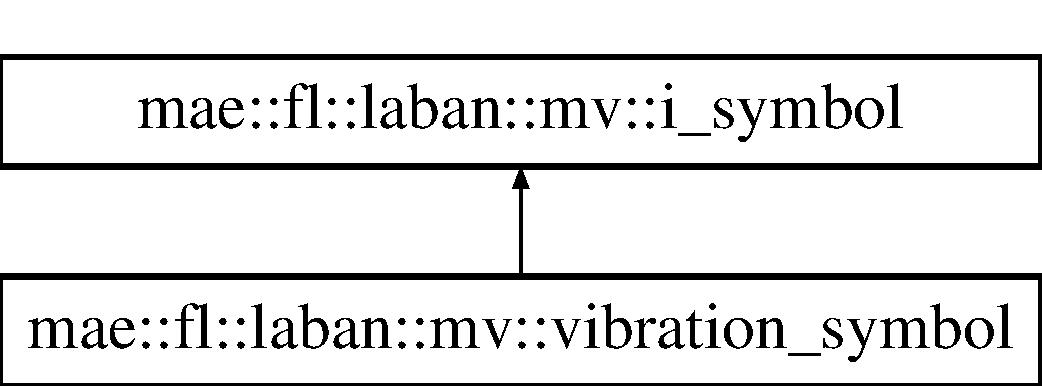
\includegraphics[height=2.000000cm]{classmae_1_1fl_1_1laban_1_1mv_1_1vibration__symbol}
\end{center}
\end{figure}
\subsection*{Public Member Functions}
\begin{DoxyCompactItemize}
\item 
\hyperlink{classmae_1_1fl_1_1laban_1_1mv_1_1vibration__symbol_af069f7c07677083e1f8dbd2ee7d06f54}{vibration\-\_\-symbol} (std\-::shared\-\_\-ptr$<$ \hyperlink{classmae_1_1fl_1_1laban_1_1mv_1_1pin}{pin} $>$ displacement1, std\-::shared\-\_\-ptr$<$ \hyperlink{classmae_1_1fl_1_1laban_1_1mv_1_1pin}{pin} $>$ displacement2, std\-::shared\-\_\-ptr$<$ \hyperlink{classmae_1_1fl_1_1laban_1_1mv_1_1i__dynamics__sign}{i\-\_\-dynamics\-\_\-sign} $>$ dynamics=nullptr)
\item 
std\-::shared\-\_\-ptr$<$ \hyperlink{classmae_1_1fl_1_1laban_1_1mv_1_1i__dynamics__sign}{i\-\_\-dynamics\-\_\-sign} $>$ \hyperlink{classmae_1_1fl_1_1laban_1_1mv_1_1vibration__symbol_a13ff61702dea27ddc05ea7a0939bf21d}{get\-\_\-dynamics} () const 
\item 
std\-::shared\-\_\-ptr$<$ \hyperlink{classmae_1_1fl_1_1laban_1_1mv_1_1pin}{pin} $>$ \hyperlink{classmae_1_1fl_1_1laban_1_1mv_1_1vibration__symbol_a529eccb1557eb44493d26ba2c3ef175a}{get\-\_\-displacement1} () const 
\item 
std\-::shared\-\_\-ptr$<$ \hyperlink{classmae_1_1fl_1_1laban_1_1mv_1_1pin}{pin} $>$ \hyperlink{classmae_1_1fl_1_1laban_1_1mv_1_1vibration__symbol_a44cd2e313eeb28b6101bc9474793a145}{get\-\_\-displacement2} () const 
\item 
virtual bool \hyperlink{classmae_1_1fl_1_1laban_1_1mv_1_1vibration__symbol_a65444ca2f4c0f7845ea3a48375379d65}{equals} (std\-::shared\-\_\-ptr$<$ \hyperlink{classmae_1_1fl_1_1laban_1_1mv_1_1i__symbol}{i\-\_\-symbol} $>$ a) const 
\item 
virtual std\-::string \hyperlink{classmae_1_1fl_1_1laban_1_1mv_1_1vibration__symbol_adaec2bb356fd6321c9585651301e1ac7}{xml} (unsigned int indent=0, std\-::string namesp=\char`\"{}\char`\"{}) const 
\item 
virtual std\-::string \hyperlink{classmae_1_1fl_1_1laban_1_1mv_1_1vibration__symbol_af8f13853392a942ceb8ceb00f3af5e47}{svg} (std\-::string identifier, double posx, double posy, double width, double height, bool left=false) const 
\item 
virtual std\-::string \hyperlink{classmae_1_1fl_1_1laban_1_1mv_1_1vibration__symbol_a6dfa83223bd1d96244268806f6d7f8b5}{str} () const 
\end{DoxyCompactItemize}
\subsection*{Friends}
\begin{DoxyCompactItemize}
\item 
\hypertarget{classmae_1_1fl_1_1laban_1_1mv_1_1vibration__symbol_a0eeedd37a3f7ed894feaed17c24199a5}{std\-::ostream \& {\bfseries operator$<$$<$} (std\-::ostream \&os, const \hyperlink{classmae_1_1fl_1_1laban_1_1mv_1_1vibration__symbol}{vibration\-\_\-symbol} \&obj)}\label{classmae_1_1fl_1_1laban_1_1mv_1_1vibration__symbol_a0eeedd37a3f7ed894feaed17c24199a5}

\item 
\hypertarget{classmae_1_1fl_1_1laban_1_1mv_1_1vibration__symbol_a80201f393f79c9c54f2c8d9b023e6955}{std\-::ostream \& {\bfseries operator$<$$<$} (std\-::ostream \&os, const std\-::shared\-\_\-ptr$<$ \hyperlink{classmae_1_1fl_1_1laban_1_1mv_1_1vibration__symbol}{vibration\-\_\-symbol} $>$ \&obj)}\label{classmae_1_1fl_1_1laban_1_1mv_1_1vibration__symbol_a80201f393f79c9c54f2c8d9b023e6955}

\end{DoxyCompactItemize}


\subsection{Constructor \& Destructor Documentation}
\hypertarget{classmae_1_1fl_1_1laban_1_1mv_1_1vibration__symbol_af069f7c07677083e1f8dbd2ee7d06f54}{\index{mae\-::fl\-::laban\-::mv\-::vibration\-\_\-symbol@{mae\-::fl\-::laban\-::mv\-::vibration\-\_\-symbol}!vibration\-\_\-symbol@{vibration\-\_\-symbol}}
\index{vibration\-\_\-symbol@{vibration\-\_\-symbol}!mae::fl::laban::mv::vibration_symbol@{mae\-::fl\-::laban\-::mv\-::vibration\-\_\-symbol}}
\subsubsection[{vibration\-\_\-symbol}]{\setlength{\rightskip}{0pt plus 5cm}mae\-::fl\-::laban\-::mv\-::vibration\-\_\-symbol\-::vibration\-\_\-symbol (
\begin{DoxyParamCaption}
\item[{std\-::shared\-\_\-ptr$<$ {\bf pin} $>$}]{displacement1, }
\item[{std\-::shared\-\_\-ptr$<$ {\bf pin} $>$}]{displacement2, }
\item[{std\-::shared\-\_\-ptr$<$ {\bf i\-\_\-dynamics\-\_\-sign} $>$}]{dynamics = {\ttfamily nullptr}}
\end{DoxyParamCaption}
)}}\label{classmae_1_1fl_1_1laban_1_1mv_1_1vibration__symbol_af069f7c07677083e1f8dbd2ee7d06f54}
Creates a vibration symbol. A vibration symbol represents an alternation between two directions which is represented by two pins.


\begin{DoxyParams}{Parameters}
{\em displacement1} & The first pin. \\
\hline
{\em displacement2} & The second pin. \\
\hline
{\em dynamics} & (optional) A dynamics sign. \\
\hline
\end{DoxyParams}


\subsection{Member Function Documentation}
\hypertarget{classmae_1_1fl_1_1laban_1_1mv_1_1vibration__symbol_a65444ca2f4c0f7845ea3a48375379d65}{\index{mae\-::fl\-::laban\-::mv\-::vibration\-\_\-symbol@{mae\-::fl\-::laban\-::mv\-::vibration\-\_\-symbol}!equals@{equals}}
\index{equals@{equals}!mae::fl::laban::mv::vibration_symbol@{mae\-::fl\-::laban\-::mv\-::vibration\-\_\-symbol}}
\subsubsection[{equals}]{\setlength{\rightskip}{0pt plus 5cm}bool mae\-::fl\-::laban\-::mv\-::vibration\-\_\-symbol\-::equals (
\begin{DoxyParamCaption}
\item[{std\-::shared\-\_\-ptr$<$ {\bf i\-\_\-symbol} $>$}]{a}
\end{DoxyParamCaption}
) const\hspace{0.3cm}{\ttfamily [virtual]}}}\label{classmae_1_1fl_1_1laban_1_1mv_1_1vibration__symbol_a65444ca2f4c0f7845ea3a48375379d65}
Returns true if signs are equal.


\begin{DoxyParams}{Parameters}
{\em a} & The sign to be compared to. \\
\hline
\end{DoxyParams}
\begin{DoxyReturn}{Returns}
True if equal. 
\end{DoxyReturn}


Implements \hyperlink{classmae_1_1fl_1_1laban_1_1mv_1_1i__symbol_a78d90af5e1da4a6561d7545a76689d0e}{mae\-::fl\-::laban\-::mv\-::i\-\_\-symbol}.

\hypertarget{classmae_1_1fl_1_1laban_1_1mv_1_1vibration__symbol_a529eccb1557eb44493d26ba2c3ef175a}{\index{mae\-::fl\-::laban\-::mv\-::vibration\-\_\-symbol@{mae\-::fl\-::laban\-::mv\-::vibration\-\_\-symbol}!get\-\_\-displacement1@{get\-\_\-displacement1}}
\index{get\-\_\-displacement1@{get\-\_\-displacement1}!mae::fl::laban::mv::vibration_symbol@{mae\-::fl\-::laban\-::mv\-::vibration\-\_\-symbol}}
\subsubsection[{get\-\_\-displacement1}]{\setlength{\rightskip}{0pt plus 5cm}std\-::shared\-\_\-ptr$<$ {\bf pin} $>$ mae\-::fl\-::laban\-::mv\-::vibration\-\_\-symbol\-::get\-\_\-displacement1 (
\begin{DoxyParamCaption}
{}
\end{DoxyParamCaption}
) const}}\label{classmae_1_1fl_1_1laban_1_1mv_1_1vibration__symbol_a529eccb1557eb44493d26ba2c3ef175a}
The first of the two alternating directions.

\begin{DoxyReturn}{Returns}
The pin. 
\end{DoxyReturn}
\hypertarget{classmae_1_1fl_1_1laban_1_1mv_1_1vibration__symbol_a44cd2e313eeb28b6101bc9474793a145}{\index{mae\-::fl\-::laban\-::mv\-::vibration\-\_\-symbol@{mae\-::fl\-::laban\-::mv\-::vibration\-\_\-symbol}!get\-\_\-displacement2@{get\-\_\-displacement2}}
\index{get\-\_\-displacement2@{get\-\_\-displacement2}!mae::fl::laban::mv::vibration_symbol@{mae\-::fl\-::laban\-::mv\-::vibration\-\_\-symbol}}
\subsubsection[{get\-\_\-displacement2}]{\setlength{\rightskip}{0pt plus 5cm}std\-::shared\-\_\-ptr$<$ {\bf pin} $>$ mae\-::fl\-::laban\-::mv\-::vibration\-\_\-symbol\-::get\-\_\-displacement2 (
\begin{DoxyParamCaption}
{}
\end{DoxyParamCaption}
) const}}\label{classmae_1_1fl_1_1laban_1_1mv_1_1vibration__symbol_a44cd2e313eeb28b6101bc9474793a145}
The second of the two alternating directions.

\begin{DoxyReturn}{Returns}
The pin. 
\end{DoxyReturn}
\hypertarget{classmae_1_1fl_1_1laban_1_1mv_1_1vibration__symbol_a13ff61702dea27ddc05ea7a0939bf21d}{\index{mae\-::fl\-::laban\-::mv\-::vibration\-\_\-symbol@{mae\-::fl\-::laban\-::mv\-::vibration\-\_\-symbol}!get\-\_\-dynamics@{get\-\_\-dynamics}}
\index{get\-\_\-dynamics@{get\-\_\-dynamics}!mae::fl::laban::mv::vibration_symbol@{mae\-::fl\-::laban\-::mv\-::vibration\-\_\-symbol}}
\subsubsection[{get\-\_\-dynamics}]{\setlength{\rightskip}{0pt plus 5cm}std\-::shared\-\_\-ptr$<$ {\bf i\-\_\-dynamics\-\_\-sign} $>$ mae\-::fl\-::laban\-::mv\-::vibration\-\_\-symbol\-::get\-\_\-dynamics (
\begin{DoxyParamCaption}
{}
\end{DoxyParamCaption}
) const}}\label{classmae_1_1fl_1_1laban_1_1mv_1_1vibration__symbol_a13ff61702dea27ddc05ea7a0939bf21d}
Returns the dynamics sign if any. Returns null otherwise.

\begin{DoxyReturn}{Returns}

\end{DoxyReturn}
\hypertarget{classmae_1_1fl_1_1laban_1_1mv_1_1vibration__symbol_a6dfa83223bd1d96244268806f6d7f8b5}{\index{mae\-::fl\-::laban\-::mv\-::vibration\-\_\-symbol@{mae\-::fl\-::laban\-::mv\-::vibration\-\_\-symbol}!str@{str}}
\index{str@{str}!mae::fl::laban::mv::vibration_symbol@{mae\-::fl\-::laban\-::mv\-::vibration\-\_\-symbol}}
\subsubsection[{str}]{\setlength{\rightskip}{0pt plus 5cm}std\-::string mae\-::fl\-::laban\-::mv\-::vibration\-\_\-symbol\-::str (
\begin{DoxyParamCaption}
{}
\end{DoxyParamCaption}
) const\hspace{0.3cm}{\ttfamily [virtual]}}}\label{classmae_1_1fl_1_1laban_1_1mv_1_1vibration__symbol_a6dfa83223bd1d96244268806f6d7f8b5}
Returns the string representation for this element.

\begin{DoxyReturn}{Returns}
The string. 
\end{DoxyReturn}


Implements \hyperlink{classmae_1_1fl_1_1laban_1_1mv_1_1i__symbol_ad254351eabf06ac945c168b24643872e}{mae\-::fl\-::laban\-::mv\-::i\-\_\-symbol}.

\hypertarget{classmae_1_1fl_1_1laban_1_1mv_1_1vibration__symbol_af8f13853392a942ceb8ceb00f3af5e47}{\index{mae\-::fl\-::laban\-::mv\-::vibration\-\_\-symbol@{mae\-::fl\-::laban\-::mv\-::vibration\-\_\-symbol}!svg@{svg}}
\index{svg@{svg}!mae::fl::laban::mv::vibration_symbol@{mae\-::fl\-::laban\-::mv\-::vibration\-\_\-symbol}}
\subsubsection[{svg}]{\setlength{\rightskip}{0pt plus 5cm}std\-::string mae\-::fl\-::laban\-::mv\-::vibration\-\_\-symbol\-::svg (
\begin{DoxyParamCaption}
\item[{std\-::string}]{identifier, }
\item[{double}]{posx, }
\item[{double}]{posy, }
\item[{double}]{width, }
\item[{double}]{height, }
\item[{bool}]{left = {\ttfamily false}}
\end{DoxyParamCaption}
) const\hspace{0.3cm}{\ttfamily [virtual]}}}\label{classmae_1_1fl_1_1laban_1_1mv_1_1vibration__symbol_af8f13853392a942ceb8ceb00f3af5e47}
Returns the S\-V\-G representation for this symbol.


\begin{DoxyParams}{Parameters}
{\em posx} & The x position. \\
\hline
{\em posy} & The y position. \\
\hline
{\em width} & The width. \\
\hline
{\em height} & The height. \\
\hline
\end{DoxyParams}
\begin{DoxyReturn}{Returns}
The S\-V\-G. 
\end{DoxyReturn}


Implements \hyperlink{classmae_1_1fl_1_1laban_1_1mv_1_1i__symbol_ae0a724c98c27c05fdde9afff99184029}{mae\-::fl\-::laban\-::mv\-::i\-\_\-symbol}.

\hypertarget{classmae_1_1fl_1_1laban_1_1mv_1_1vibration__symbol_adaec2bb356fd6321c9585651301e1ac7}{\index{mae\-::fl\-::laban\-::mv\-::vibration\-\_\-symbol@{mae\-::fl\-::laban\-::mv\-::vibration\-\_\-symbol}!xml@{xml}}
\index{xml@{xml}!mae::fl::laban::mv::vibration_symbol@{mae\-::fl\-::laban\-::mv\-::vibration\-\_\-symbol}}
\subsubsection[{xml}]{\setlength{\rightskip}{0pt plus 5cm}std\-::string mae\-::fl\-::laban\-::mv\-::vibration\-\_\-symbol\-::xml (
\begin{DoxyParamCaption}
\item[{unsigned int}]{indent = {\ttfamily 0}, }
\item[{std\-::string}]{namesp = {\ttfamily \char`\"{}\char`\"{}}}
\end{DoxyParamCaption}
) const\hspace{0.3cm}{\ttfamily [virtual]}}}\label{classmae_1_1fl_1_1laban_1_1mv_1_1vibration__symbol_adaec2bb356fd6321c9585651301e1ac7}
Returns the X\-M\-L representation for this element.


\begin{DoxyParams}{Parameters}
{\em indent} & The applied indent. \\
\hline
{\em namesp} & The prefixed X\-M\-L namespace.\\
\hline
\end{DoxyParams}
\begin{DoxyReturn}{Returns}
The X\-M\-L string. 
\end{DoxyReturn}


Implements \hyperlink{classmae_1_1fl_1_1laban_1_1mv_1_1i__symbol_a05d0b0c74bad854d5e9e3291bbd87b0d}{mae\-::fl\-::laban\-::mv\-::i\-\_\-symbol}.



The documentation for this class was generated from the following files\-:\begin{DoxyCompactItemize}
\item 
src/mae/fl/laban/mv/vibration\-\_\-symbol.\-hpp\item 
src/mae/fl/laban/mv/vibration\-\_\-symbol.\-cpp\end{DoxyCompactItemize}

%--- End generated contents ---

% Index
\newpage
\phantomsection
\addcontentsline{toc}{chapter}{Index}
\printindex

\end{document}
